\part{Calculus III}


\apexchapter{Vectors}{chapter:vectors}

This chapter introduces a new mathematical object, the \sword{vector}. Defined in \autoref{sec:vector_intro}, we will see that vectors provide a powerful language for describing quantities that have magnitude and direction aspects. A simple example of such a quantity is force: when applying a force, one is generally interested in how much force is applied (i.e., the magnitude of the force) and the direction in which the force was applied. Vectors will play an important role in many of the subsequent chapters in this text. 

This chapter begins with moving our mathematics out of the plane and into ``space.'' That is, we begin to think mathematically not only in two dimensions, but in three. With this foundation, we can explore vectors both in the plane and in space. 

\section{Introduction to Cartesian Coordinates in Space}\label{sec:space_coord}

Up to this point in this text we have considered mathematics in a 2-dimensional world. We have plotted graphs on the $x$-$y$ plane using rectangular and polar coordinates and found the area of regions in the plane. We have considered properties of \emph{solid} objects, such as volume and surface area, but only by first defining a curve in the plane and then rotating it out of the plane.

While there is wonderful mathematics to explore in ``2D,'' we live in a ``3D'' world and eventually we will want to apply mathematics involving this third dimension. In this section we introduce Cartesian coordinates in space and explore basic surfaces. This will lay a foundation for much of what we do in the remainder of the text.\\

Each point $P$ in space can be represented with an ordered triple, $P=(a,b,c)$, where $a$, $b$ and $c$ represent the relative position of $P$ along the $x$-, $y$- and $z$-axes, respectively. Each axis is perpendicular to the other two.

Visualizing points in space on paper can be problematic, as we are trying to represent a 3-dimensional concept on a 2-dimensional medium. We cannot draw three lines representing the three axes in which each line is perpendicular to the other two. Despite this issue, standard conventions exist for plotting shapes in space that we will discuss that are more than adequate.

\mtable{Illustrating the right hand rule.  Figure courtesy of \href{https://commons.wikimedia.org/wiki/File:Right_hand_rule_simple.png}{user:Schorschi2} / \href{http://commons.wikimedia.org/}{Wikimedia Commons} / Public Domain.}{fig:right_hand_rule}{\centering
\begin{tikzpicture}[baseline=-10ex]
 \draw[->](0,0)--(0,1)node[above]{$z$};
 \draw[->](0,0)--(-.5,-.3)node[below left]{$x$};
 \draw[->](0,0)--(.5,-.3)node[below right]{$y$};
\node at(2,.5){\rotatebox{41}{\includegraphics[width=.5\marginparwidth]{figures/raw/Right_hand_rule_simple.png}}};
\end{tikzpicture}
\vspace{-2\baselineskip}}

One convention is that the axes must conform to the \textbf{right hand rule}. This rule states that when the fingers of the right hand extend in the direction of the positive $x$-axis and curve toward the positive $y$-axis, then the extended thumb will point in the direction of the positive $z$-axis. (It may take some thought to verify this, but this system is inherently different from the one created by using the ``left hand rule.'')
Another way to view the rule is that when the index finger of the right hand extends in the direction of the positive $x$-axis, and the middle finger (bent ``inward'' so it is perpendicular to the palm) points along the positive $y$-axis, then the extended thumb will point in the direction of the positive $z$-axis.%
\index{right hand rule!of Cartesian coordinates}

As long as the coordinate axes are positioned so that they follow this rule, it does not matter how the axes are drawn on paper. There are two popular methods that we briefly discuss.
\mtable{Plotting the point $P=(2,1,3)$ in space.}{fig:cartcoord1}{%
\myincludeasythree{width=\marginparwidth,
3Droll=0,
3Dortho=0.0045,
3Dc2c=11 5 2.8,
3Dcoo=0 0 0,
3Droo=200}{width=\marginparwidth}{figures/figcartcoord1_3D}}

In \autoref{fig:cartcoord1} we see the point $P=(2,1,3)$ plotted on a set of axes. The basic convention here is that the $x$-$y$ plane is drawn in its standard way, with the $z$-axis down to the left. The perspective  is that the paper represents the $x$-$y$ plane and the positive $z$ axis is coming up, off the page. This method is preferred by many engineers. Because it can be hard to tell where a single point lies in relation to all the axes, dashed lines have been added to let one see how far along each axis the point lies.

One can also consider the $x$-$y$ plane as being a horizontal plane in, say, a room, where the positive $z$-axis is pointing up. When one steps back and looks at this room, one might draw the axes as shown in \autoref{fig:cartcoord2}. The same point $P$ is drawn, again with dashed lines. This point of view is preferred by most mathematicians, and is the convention adopted by this text.

Just as the $x$- and $y$-axes divide the plane into four quadrants, the $x$-, $y$-, and $z$-coordinate planes divide space into eight octants.  The octant in which $x$, $y$, and $z$ are positive is called the first octant.  We will not give special names for the other seven octants.

\mtable{Plotting the point $P=(2,1,3)$ in space with a perspective used in this text.}{fig:cartcoord2}{%
\myincludeasythree{width=\marginparwidth,
3Droll=0,
3Dortho=0.004,
3Dc2c=0.6666666865348816 0.6666666865348816 0.3333333730697632,
3Dcoo=16.7497615814209 8.84995174407959 40.36832046508789,
3Droo=129.79413580025474}{width=\marginparwidth}{figures/figcartcoord2_3D}}

\subsection{Measuring Distances}

It is of critical importance to know how to measure distances between points in space. The formula for doing so is based on measuring distance in the plane and the Pythagorean theorem, and is known (in both contexts) as the Euclidean measure of distance.

\begin{definition}[Distance In Space]\label{def:space_distance}
Let $P=(x_1,y_1,z_1)$ and $Q = (x_2,y_2,z_2)$ be points in space. The distance $D$ between $P$ and $Q$ is \index{distance!between points in space}
\[D = \sqrt{(x_2-x_1)^2+(y_2-y_1)^2+(z_2-z_1)^2}.\]
\end{definition}

We refer to the line segment that connects points $P$ and $Q$ in space as $\overline{PQ}$, and refer to the length of this segment as $\norm{\overline{PQ}}$. The above distance formula allows us to compute the length of this segment.\\

\begin{example}[Length of a line segment]\label{ex_space1}
Let $P = (1,4,-1)$ and let $Q = (2,1,1)$. Draw the line segment $\overline{PQ}$ and find its length.
\solution
The points $P$ and $Q$ are plotted in \autoref{fig:space1}; no special consideration needs to be made to draw the line segment connecting these two points; simply connect them with a straight line. One \emph{cannot} actually measure this line on the page and deduce anything meaningful; its true length must be measured analytically. Applying \autoref{def:space_distance}, we have
%
\mtable{Plotting points $P$ and $Q$ in \autoref{ex_space1}.}{fig:space1}{%
\myincludeasythree{width=\marginparwidth,
3Droll=0,
3Dortho=0.0044,
3Dc2c=0.6474442481994629 0.6759132146835327 0.35207563638687134,
3Dcoo=32.306640625 39.99113082885742 5.668694019317627,
3Droo=113.20770262248418}{width=\marginparwidth}{figures/figspace1_3D}}
%
\[
\norm{\overline{PQ}}= \sqrt{(2-1)^2+(1-4)^2+(1-(-1))^2} = \sqrt{14}%\approx 3.74
.
\]
\end{example}

\subsection{Spheres}

\index{sphere}Just as a circle is the set of all points in the \emph{plane} equidistant from a given point (its center), a sphere is the set of all points in \emph{space} that are equidistant from a given point. \autoref{def:space_distance} allows us to write an equation of the sphere.

We start with a point $C = (a,b,c)$ which is to be the center of a sphere with radius $r$. If a point $P=(x,y,z)$ lies on the sphere, then $P$ is $r$ units from $C$; that is, 
\[\norm{\overline{PC}}= \sqrt{(x-a)^2+(y-b)^2+(z-c)^2} = r.\]
Squaring both sides, we get the standard equation of a sphere in space with center at $C=(a,b,c)$ with radius $r$, as given in the following Key Idea.

\begin{keyidea}[Standard Equation of a Sphere in Space]\label{idea:sphere}
The standard equation of the sphere with radius $r$, centered at $C=(a,b,c)$, is
\[(x-a)^2+(y-b)^2+(z-c)^2=r^2.\]
\end{keyidea}

\youtubeVideo{fE_PWxyohXQ}{Example of Equation of a Sphere}

\begin{example}[Equation of a sphere]\label{ex_space2}
Find the center and radius of the sphere defined by $x^2+2x+y^2-4y+z^2-6z=2$.
\solution
To determine the center and radius, we must put the equation in standard form. This requires us to complete the square (three times).
\begin{align*}
x^2+2x+y^2-4y+z^2-6z&=2 \\
(x^2+2x+1) + (y^2-4y+4)+ (z^2-6z+9) - 14 &= 2\\
(x+1)^2 + (y-2)^2 + (z-3)^2 &= 16
\end{align*}
The sphere is centered at $(-1,2,3)$ and has a radius of 4.
\end{example}

The equation of a sphere is an example of an implicit function defining a surface in space. In the case of a sphere, the variables $x$, $y$ and $z$ are all used. We now consider situations where surfaces are defined where one or two of these variables are absent.

\subsection{Introduction to Planes in Space}

The coordinate axes naturally define three planes (shown in \autoref{fig:coordplanes}), the \textbf{coordinate planes}: the $x$-$y$ plane, the $y$-$z$ plane and the $x$-$z$ plane. The $x$-$y$ plane is characterized as the set of all points in space where the $z$-value is 0. %(Likewise, the $x$-$z$ plane is all points where the $y$-value is 0.) 
\index{planes!coordinate plane}\index{planes!introduction}
This, in fact, gives us an equation that describes this plane: $z=0$. Likewise, the $x$-$z$ plane is all points where the $y$-value is 0, characterized by $y=0$.\\

\noindent\begin{minipage}[t]{\linewidth}\noindent%
\captionsetup{type=figure}%
\flushinner{%
%\noindent\begin{minipage}{\textwidth}
\begin{tabular}{ccc}
\myincludeasythree{width=.3\textwidth,
3Droll=0,
3Dortho=0.004,
3Dc2c=4 4 2,
3Dcoo=0 0 0,
3Droo=150}{width=.3\textwidth}{figures/figspacexy_3D}
&
\myincludeasythree{width=.3\textwidth,
3Droll=0,
3Dortho=0.004,
3Dc2c=4 4 2,
3Dcoo=0 0 0,
3Droo=150}{width=.3\textwidth}{figures/figspaceyz_3D}
&
\myincludeasythree{width=.3\textwidth,
3Droll=0,
3Dortho=0.004,
3Dc2c=4 4 2,
3Dcoo=0 0 0,
3Droo=150}{width=.3\textwidth}{figures/figspacexz_3D}
\\
the $x$-$y$ plane & the $y$-$z$ plane & the $x$-$z$ plane
\end{tabular}}
\caption{The coordinate planes.}\label{fig:coordplanes}
\end{minipage}

% todo Tim this would look better if the bl-ue plane would not stop exactly at the z-axis and if the tip of the x-axis would stick out
\mtable{The plane $x=2$.}{fig:space2}{%
\myincludeasythree{width=\marginparwidth,
3Droll=0,
3Dortho=0.0044,
3Dc2c=4 4 2,
3Dcoo=0 0 0,
3Droo=150}{width=\marginparwidth}{figures/figspace2_3D}}

% todo Mention the general drawing trick: if a plane is parallel to a coordinate axis, draw grid lines parallel to that axis onto the plane.  Also draw an example of an oblique plane.
\begin{example}[A plane in three dimensions]\label{ex_space_x_is_two}
The equation $x=2$ describes all points in space where the $x$-value is 2. This is a plane, parallel to the $y$-$z$ coordinate plane, shown in \autoref{fig:space2}.
\end{example}

\begin{example}[Regions defined by planes]\label{ex_space3}
Sketch the region defined by the inequalities $-1\leq y\leq 2$.
\solution
%
\mtable{Sketching the boundaries of a region in \autoref{ex_space3}.}{fig:space3}{%
\myincludeasythree{width=\marginparwidth,
3Droll=0,
3Dortho=0.0044,
3Dc2c=4 2.5 2,
3Dcoo=0 0 0,
3Droo=150}{width=\marginparwidth}{figures/figspace3_3D}}
%
The region is all points between the planes $y=-1$ and $y=2$. These planes are sketched in \autoref{fig:space3}, which are parallel to the $x$-$z$ plane. Thus the region extends infinitely in the $x$ and $z$ directions, and is bounded by planes in the $y$ direction.
\end{example}

\subsection{Cylinders}

The equation $x=1$ obviously lacks the $y$ and $z$ variables, meaning it defines points where the $y$ and $z$ coordinates can take on any value. Now consider the equation $x^2+y^2=1$ \emph{in space.} In \emph{the plane}, this equation describes a circle of radius 1, centered at the origin. In space, the $z$ coordinate is not specified, meaning it can take on any value. In \autoref{fig:spacecylinder1} (a), we show part of the graph of the equation $x^2+y^2=1$ by sketching 3 circles: the bottom one has a constant $z$-value of $-1.5$, the middle one has a $z$-value of 0 and the top circle has a $z$-value of 1. By plotting \emph{all} possible $z$-values, we get the  surface shown in \autoref{fig:spacecylinder1} (b). This surface looks like a ``tube,'' or a ``cylinder'', which leads to our next definition.
%; mathematicians call this surface a \textbf{cylinder} for an entirely different reason.

\mtable{Sketching $x^2+y^2=1$.}{fig:spacecylinder1}{%
\myincludeasythree{width=\marginparwidth,
3Droll=0,
3Dortho=0.004,
3Dc2c=4 4 2,
3Dcoo=0 0 0,
3Droo=150}{width=\marginparwidth}{figures/figspacecylinder1_3D}
\\[5pt](a)\\[5pt]
\myincludeasythree{width=\marginparwidth,
3Droll=0,
3Dortho=0.004,
3Dc2c=4 4 2,
3Dcoo=0 0 0,
3Droo=150}{width=\marginparwidth}{figures/figspacecylinder1b_3D}
\\[5pt](b)}

\begin{definition}[Cylinder]\label{def:cylinder}
Let $C$ be a curve in a plane and let $L$ be a line not parallel to $C$. A \textbf{cylinder} is the set of all lines parallel to $L$ that pass through $C$. The curve $C$ is the \textbf{directrix} of the cylinder, and the lines are the \textbf{rulings}.\index{cylinder}\index{directrix}
\end{definition}

In this text, we consider curves $C$ that lie in planes parallel to one of the coordinate planes, and lines $L$ that are perpendicular to these planes, forming \textbf{right cylinders}. Thus the directrix can be defined using equations involving 2 variables, and the rulings will be parallel to the axis of the 3$^\text{rd}$ variable.

In the example preceding the definition, the curve $x^2+y^2=1$ in the $x$-$y$ plane is the directrix and the rulings are lines parallel to the $z$-axis. (Any circle shown in \autoref{fig:spacecylinder1} can be considered a directrix; we simply choose the one where $z=0$.) Sample rulings can also be viewed in part (b) of the figure. More examples will help us understand this definition.

\begin{example}[Graphing cylinders]\label{ex_space4}
Graph the following cylinders.
\[\text{1.}\quad z=y^2\qquad \text{2.}\quad x=\sin z\]
\solution
\begin{enumerate}
	\item We can view the equation $z=y^2$ as a parabola in the $y$-$z$ plane, as illustrated in \autoref{fig:space4a} (a). As $x$ does not appear in the equation, the rulings are lines through this parabola parallel to the $x$-axis, shown in (b). These rulings give a general idea as to what the surface looks like, drawn in (c).
	
{\centering
\captionsetup{type=figure}%
\begin{tabular}{ccc}
\myincludeasythree{width=.3\linewidth,
3Droll=0,
3Dortho=0.004,
3Dc2c=4 4 2,
3Dcoo=0 0 75,
3Droo=150}{width=.3\linewidth}{figures/figspace4a_3D}
 &
\myincludeasythree{width=.3\linewidth,
3Droll=0,
3Dortho=0.004,
3Dc2c=4 4 2,
3Dcoo=0 0 75,
3Droo=150}{width=.3\linewidth}{figures/figspace4b_3D}
 &
\myincludeasythree{width=.3\linewidth,
3Droll=0,
3Dortho=0.004,
3Dc2c=4 4 2,
3Dcoo=0 0 75,
3Droo=150}{width=.3\linewidth}{figures/figspace4c_3D}
\\(a) & (b) & (c)
\end{tabular}
\caption{Sketching the cylinder defined by $z=y^2$.}\label{fig:space4a}
}% end centering
	
	\item		We can view the equation $x=\sin z$ as a sine curve that exists in the $x$-$z$ plane, as shown in \autoref{fig:space4b} (a). The rules are parallel to the $y$ axis as the variable $y$ does not appear in the equation $x=\sin z$; some of these are shown in part (b). The surface is shown in part (c) of the figure. 

{\centering
\captionsetup{type=figure}%
\begin{tabular}{ccc}
\myincludeasythree{width=.3\linewidth,
3Droll=0,
3Dortho=0.0045,
3Dc2c=4 4 3,
3Dcoo=0 0 0,
3Droo=150}{width=.3\linewidth}{figures/figspace4d_3D}
 &
\myincludeasythree{width=.3\linewidth,
3Droll=0,
3Dortho=0.0045,
3Dc2c=4 4 3,
3Dcoo=0 0 0,
3Droo=150}{width=.3\linewidth}{figures/figspace4e_3D} 
&
\myincludeasythree{width=.3\linewidth,
3Droll=0,
3Dortho=0.0045,
3Dc2c=4 4 3,
3Dcoo=0 0 0,
3Droo=150}{width=.3\linewidth}{figures/figspace4f_3D}
\\(a) & (b) & (c)
\end{tabular}
\caption{Sketching the cylinder defined by $x=\sin z$.}\label{fig:space4b}
}% end centering
\end{enumerate}
\end{example}

\subsection{Surfaces of Revolution}

\mtable{Introducing surfaces of revolution.}{fig:surf_rev_intro}{%
\myincludeasythree{width=\marginparwidth,
3Droll=0,
3Dortho=0.0045,
3Dc2c=.395 .79 .356,
3Dcoo=75 0 0,
3Droo=130}{width=\marginparwidth}{figures/figsurf_rev_intro_3D}
\\(a)\\
\myincludeasythree{width=\marginparwidth,
3Droll=0,
3Dortho=0.0045,
3Dc2c=.395 .79 .356,
3Dcoo=75 0 0,
3Droo=130}{width=\marginparwidth}{figures/figsurf_rev_introb_3D}
\\(b)}

One of the applications of integration we learned previously was to find the volume of solids of revolution --- solids formed by revolving a curve about a horizontal or vertical axis. We now consider how to find the equation of the surface of such a solid.

Consider the surface formed by revolving the curve $y=\sqrt{x}$ in the $x$-$y$ plane about the $x$-axis. Cross-sections of this surface parallel to the $y$-$z$ plane are circles, as shown in \autoref{fig:surf_rev_intro}(a). Each circle has equation of the form $y^2+z^2=r^2$ for some radius $r$. The radius is a function of $x$; in fact, it is $r(x) = \sqrt{x}$. Thus the equation of the surface shown in \autoref{fig:surf_rev_intro}(b) is $y^2+z^2=(\sqrt{x})^2.$

We generalize the above principles to give the equations of surfaces formed by revolving curves about the coordinate axes.

\begin{keyidea}[Surfaces of Revolution, Part 1]\label{idea:surf_of_revol}
Let $r$ be a radius function. \index{surface of revolution}
\begin{enumerate}
	\item The equation of the surface formed by revolving $y=r(x)$ or $z=r(x)$ about the $x$-axis is $y^2+z^2=r(x)^2$.
	\item The equation of the surface formed by revolving $x=r(y)$ or $z=r(y)$ about the $y$-axis is $x^2+z^2=r(y)^2$.
	\item The equation of the surface formed by revolving $x=r(z)$ or $y=r(z)$ about the $z$-axis is $x^2+y^2=r(z)^2$.
\end{enumerate}
\end{keyidea}

\begin{example}[Finding equation of a surface of revolution]\label{ex_surfrev1}
Let $y=\sin z$ on $[0,\pi]$. Find the equation of the surface of revolution formed by revolving $y=\sin z$ about the $z$-axis.
\solution
Using \autoref{idea:surf_of_revol}, we find the surface has equation $x^2+y^2=\sin^2z$. The curve is sketched in \autoref{fig:surfrev1}(a) and the surface is drawn in \autoref{fig:surfrev1}(b).

Note how the surface (and hence the resulting equation) is the same if we began with the curve $x=\sin z$, which is also drawn in \autoref{fig:surfrev1}(a).
\end{example}

\mtable[2\baselineskip]{Revolving $y=\sin z$ about the $z$-axis in \autoref{ex_surfrev1}.}{fig:surfrev1}{%
\myincludeasythree{width=.8\marginparwidth,
3Droll=0,
3Dortho=0.0046,
3Dc2c=.66 .67 .32,
3Dcoo=0 0 75,
3Droo=130}{width=.8\marginparwidth}{figures/figsurfrev1a_3D}
\\(a)\\
\myincludeasythree{width=.8\marginparwidth,
3Droll=0,
3Dortho=0.0046,
3Dc2c=.66 .67 .32,
3Dcoo=0 0 75,
3Droo=130}{width=.8\marginparwidth}{figures/figsurfrev1b_3D}
\\(b)}

This particular method of creating surfaces of revolution is limited. For instance, in \autoref{ex_shell4} of \autoref{sec:shell_method} we found the volume  of the solid formed by revolving $y=\sin x$ about the $y$-axis. Our current method of forming surfaces can only rotate $y=\sin x$ about the $x$-axis. Trying to rewrite $y=\sin x$ as a function of $y$ is not trivial, as simply writing $x=\sin^{-1}y$ only gives part of the region we desire.

What we desire is a way of writing the surface of revolution formed by rotating $y=f(x)$ about the $y$-axis. We start by first recognizing this surface is the same as revolving $z=f(x)$ about the $z$-axis, although it has a different orientation. This will give us a more natural way of viewing the surface. 

A value of $x$ is a measurement of distance from the $z$-axis. At the distance $r$, we plot a $z$-height of $f(r)$. When rotating $f(x)$ about the $z$-axis, we want all points a distance of $r$ from the $z$-axis in the $x$-$y$ plane to have a $z$-height of $f(r)$. All such points satisfy the equation $r^2=x^2+y^2$; hence $r=\sqrt{x^2+y^2}$. Replacing $r$ with $\sqrt{x^2+y^2}$ in $f(r)$ gives $z=f(\sqrt{x^2+y^2})$. This is the equation of the surface.

\begin{keyidea}[Surfaces of Revolution, Part 2]\label{idea:surf_of_revol2}
Let $z=f(x)$, $x\geq 0$, be a curve in the $x$-$z$ plane. The surface formed by revolving this curve about the $z$-axis has equation $z=f\bigl(\sqrt{x^2+y^2}\bigr)$.\index{surface of revolution}
\end{keyidea}

\mtable[\baselineskip]{Revolving $z=\sin x$ about the $z$-axis in \autoref{ex_surfrev2}.}{fig:surfrev2}{%
\myincludeasythree{width=.8\marginparwidth,
3Droll=0,
3Dortho=0.0046,
3Dc2c=.66 .67 .32,
3Dcoo=0 0 10,
3Droo=130}{width=.8\marginparwidth}{figures/figsurfrev2a_3D}
\\(a)\\[5pt]
\myincludeasythree{width=.8\marginparwidth,
3Droll=0,
3Dortho=0.0046,
3Dc2c=.66 .67 .32,
3Dcoo=0 0 25,
3Droo=130}{width=.8\marginparwidth}{figures/figsurfrev2b_3D}
\\(b)}
%
\begin{example}[Finding equation of surface of revolution]\label{ex_surfrev2}
Find the equation of the surface found by revolving $z=\sin x$ about the $z$-axis.
\solution
Using \autoref{idea:surf_of_revol2}, the surface has equation $z=\sin\bigl(\sqrt{x^2+y^2}\bigr)$. The curve and surface are graphed in \autoref{fig:surfrev2}.
\end{example}

\subsection{Quadric Surfaces}

Spheres, planes and cylinders are important surfaces to understand. We now consider one last type of surface, a \textbf{quadric surface}. The definition may look intimidating, but we will show how to analyze these surfaces in an illuminating way.

\begin{definition}[Quadric Surface]\label{def:quadric}
A \textbf{quadric surface} is the graph of the general second-degree equation in three variables:
\index{quadric surface!definition}
\[Ax^2+By^2+Cz^2+Dxy+Exz+Fyz+Gx+Hy+Iz+J=0.\]
\end{definition}

When the coefficients $D$, $E$ or $F$ are not zero, the basic shapes of the quadric surfaces are rotated in space. We will focus on quadric surfaces where these coefficients are 0; we will not consider rotations. There are six basic quadric surfaces: the elliptic paraboloid, elliptic cone, ellipsoid, hyperboloid of one sheet, hyperboloid of two sheets, and the hyperbolic paraboloid.

\mtable[5\baselineskip]{The elliptic paraboloid $z=x^2/4+y^2$.}{fig:quadric1}{%
\myincludeasythree{width=.8\marginparwidth,
3Droll=0,
3Dortho=0.00617163721472025,
3Dc2c=0.6847050189971924 0.6847050189971924 0.24971593916416168,
3Dcoo=-6.000957012176514 2.2318615913391113 85.33463287353516,
3Droo=150}{width=.8\marginparwidth}{figures/figquadric_parb_3D}}

We study each shape by considering \textbf{traces}, \index{trace}\index{quadric surface!trace}%
that is, intersections of each surface with a plane parallel to a coordinate plane. For instance, consider the elliptic paraboloid $z= x^2/4+y^2$, shown in \autoref{fig:quadric1}. If we intersect this shape with the plane $z=d$\ \  (i.e., replace $z$ with $d$), we have the equation:
\begin{align*}
d &= \frac{x^2}4+y^2.
\intertext{Divide both sides by $d$:}
1 &= \frac{x^2}{4d} + \frac{y^2}{d}.
\end{align*}
This describes an ellipse --- so cross sections parallel to the $x$-$y$ coordinate plane are ellipses. This ellipse is drawn in the figure.

Now consider cross sections parallel to the $x$-$z$ plane. For instance, letting $y=0$ gives the equation $z=x^2/4$, clearly a parabola. Intersecting with the plane $x=0$ gives a cross section defined by $z=y^2$, another parabola. These parabolas are also sketched in the figure. 

Thus we see where the elliptic paraboloid gets its name: some cross sections are ellipses, and others are parabolas.

Such an analysis can be made with each of the quadric surfaces. We give a sample equation of each, provide a sketch with representative traces, and describe these traces.

%\clearpage
\exercisegeometry
\pagestyle{exercise}

\index{quadric surface!gallery|(}
\noindent
\begin{minipage}{1.1\linewidth}
 \captionsetup{type=figure}%
 \noindent%
 \begin{minipage}[c]{.35\linewidth}
  \mbox{}\\
  \myincludeasythree{width=\marginparwidth,
3Droll=0,
3Dortho=0.005,
3Dc2c=.85 .85 .31,
3Dcoo=0 0 75,
3Droo=150}{width=\marginparwidth}{figures/figquadric_par_3D}
 \end{minipage}%
 \begin{minipage}[c]{.2\linewidth}
  \mbox{}\\
  \begin{tabular}{cc}
   \textbf{Plane}  & \textbf{Trace} \\\midrule
   $x=d$ & Parabola \\
   $y=d$ & Parabola \\
   $z=d$ & Ellipse
  \end{tabular}
 \end{minipage}%
 \begin{minipage}[c]{.45\linewidth}
  \mbox{}\\
  \myincludeasythree{width=\marginparwidth,
3Droll=0,
3Dortho=0.005,
3Dc2c=.85 .85 .31,
3Dcoo=0 0 75,
3Droo=150}{width=\marginparwidth}{figures/figquadric_parb_3D}
 \end{minipage}
 \caption{\quad\textbf{Elliptic Paraboloid}\qquad$z=\dfrac{x^2}{a^2}+\dfrac{y^2}{b^2}$}
 \label{fig_elliptic_paraboloid}
 \bigskip
 \begin{minipage}{.75\linewidth}
  One variable in the equation of the elliptic paraboloid will be raised to the first power; above, this is the $z$ variable. The paraboloid will ``open'' in the direction of this variable's axis. Thus $x= y^2/a^2+z^2/b^2$ is an elliptic paraboloid that opens along the $x$-axis.\bigskip

  Multiplying the right hand side by $(-1)$ defines an elliptic paraboloid that ``opens'' in the opposite direction.\index{quadric surface!elliptic paraboloid}
 \end{minipage}
\end{minipage}

\vfill
\noindent\hrulefill
\vfill

\noindent
\begin{minipage}{1.1\linewidth}
 \captionsetup{type=figure}%
 \noindent%
 \begin{minipage}[c]{.25\linewidth}
  \mbox{}\\
  \myincludeasythree{width=\marginparwidth,
3Droll=0,
3Dortho=0.0067,
3Dc2c=.68 .68 .25,
3Dcoo=0 0 0,
3Droo=150}{width=\marginparwidth}{figures/figquadric_cone_3D}
 \end{minipage}%
 \begin{minipage}[c]{.2\linewidth}
  \begin{tabular}{cc}
   \textbf{Plane}  & \textbf{Trace} \\\midrule
   $x=0$ & Crossed Lines \\
   $y=0$ & Crossed Lines\\\\
   $x=d$ & Hyperbola\\
   $y=d$ & Hyperbola\\
   $z=d$ & Ellipse
  \end{tabular}
 \end{minipage}%
 \begin{minipage}[c]{.55\linewidth}
  \mbox{}\\
  \myincludeasythree{width=.8\marginparwidth,
3Droll=0,
3Dortho=0.0067,
3Dc2c=.68 .68 .25,
3Dcoo=0 0 0,
3Droo=150}{width=.8\marginparwidth}{figures/figquadric_coneb_3D}
\ %
  \myincludeasythree{width=.8\marginparwidth,
3Droll=0,
3Dortho=0.0067,
3Dc2c=.68 .68 .25,
3Dcoo=0 0 0,
3Droo=150}{width=.8\marginparwidth}{figures/figquadric_conec_3D}
 \end{minipage}
 \caption{\quad\textbf{Elliptic Cone}\qquad$z^2=\dfrac{x^2}{a^2}+\dfrac{y^2}{b^2}$}
 \label{fig_elliptic_cone}
 \bigskip
 \begin{minipage}{.75\linewidth}
  One can rewrite the equation as $z^2-x^2/a^2-y^2/{b^2} = 0$. The one variable with a positive coefficient corresponds to the axis that the cones ``open'' along. \index{quadric surface!elliptic cone}
 \end{minipage}
\end{minipage}

\clearpage

\noindent
\begin{minipage}{1.1\linewidth}
 \captionsetup{type=figure}%
 \noindent%
 \begin{minipage}[c]{.4\linewidth}
  \mbox{}\\
  \myincludeasythree{width=\marginparwidth,
3Droll=0,
3Dortho=0.005,
3Dc2c=.4 .87 .3,
3Dcoo=0 0 0,
3Droo=150}{width=\marginparwidth}{figures/figquadric_hyp_par_3D}
 \end{minipage}%
 \begin{minipage}[c]{.4\linewidth}
  \mbox{}\\
  \begin{tabular}{cc}
   \textbf{Plane}  & \textbf{Trace} \\\midrule
   $x=d$ & Parabola\\
   $y=d$ & Parabola\\
   $z=d$ & Hyperbola
  \end{tabular}
 \end{minipage}
 \bigskip\\
 \begin{minipage}[c]{.4\linewidth}
  \mbox{}\\
  \myincludeasythree{width=\marginparwidth,
3Droll=0,
3Dortho=0.005,
3Dc2c=.4 .87 .3,
3Dcoo=0 0 0,
3Droo=150}{width=\marginparwidth}{figures/figquadric_hyp_parb_3D}
 \end{minipage}%
 \begin{minipage}[c]{.4\linewidth}
  \mbox{}\\
  \myincludeasythree{width=\marginparwidth,
3Droll=0,
3Dortho=0.005,
3Dc2c=.4 .87 .3,
3Dcoo=0 0 0,
3Droo=150}{width=\marginparwidth}{figures/figquadric_hyp_parc_3D}
 \end{minipage}
 \caption{\quad\textbf{Hyperbolic Paraboloid}\qquad$z=\dfrac{x^2}{a^2}-\dfrac{y^2}{b^2}$}
 \label{fig_hyperbolic_paraboloid}
 \bigskip
  The parabolic traces will open along the axis of the one variable that is raised to the first power.\index{quadric surface!hyperbolic paraboloid}
\end{minipage}

\vfill
\noindent\hrulefill
\vfill

\noindent
\begin{minipage}{1.1\linewidth}
 \captionsetup{type=figure}%
 \noindent%
 \begin{minipage}[c]{.3\linewidth}
  \mbox{}\\
  \myincludeasythree{width=\marginparwidth,
3Droll=0,
3Dortho=0.005,
3Dc2c=.85 .85 .31,
3Dcoo=0 0 0,
3Droo=150}{width=\marginparwidth}{figures/figquadric_ellipsoid_3D}
 \end{minipage}%
 \begin{minipage}[c]{.2\linewidth}
  \begin{tabular}{cc}
   \textbf{Plane}  & \textbf{Trace} \\\midrule
   $x=d$ & Ellipse\\
   $y=d$ & Ellipse\\
   $z=d$ & Ellipse
  \end{tabular}
 \end{minipage}%
 \begin{minipage}[c]{.5\linewidth}
  \mbox{}\\
  \myincludeasythree{width=\marginparwidth,
3Droll=0,
3Dortho=0.005,
3Dc2c=.85 .85 .31,
3Dcoo=0 0 0,
3Droo=150}{width=\marginparwidth}{figures/figquadric_ellipsoidb_3D}
 \end{minipage}
 \caption{\quad\textbf{Ellipsoid}\qquad$\dfrac{x^2}{a^2}+\dfrac{y^2}{b^2}+\dfrac{z^2}{c^2}=1$}
 \bigskip
  If $a=b=c\neq0$, the ellipsoid is a sphere with radius $a$; compare to \autoref{idea:sphere}.\index{quadric surface!ellipsoid}\index{quadric surface!sphere}
\end{minipage}

\clearpage

\noindent
\begin{minipage}{1.1\linewidth}
 \captionsetup{type=figure}%
 \noindent%
 \begin{minipage}[c]{.35\linewidth}
  \mbox{}\\
  \myincludeasythree{width=\marginparwidth,
3Droll=0,
3Dortho=0.005,
3Dc2c=.85 .85 .31,
3Dcoo=0 0 0,
3Droo=150}{width=\marginparwidth}{figures/figquadric_hyp_one_sheet_3D}
 \end{minipage}%
 \begin{minipage}[c]{.23\linewidth}
  \mbox{}\\
  \begin{tabular}{cc}
   \textbf{Plane}  & \textbf{Trace} \\\midrule
   $x=d$ & Hyperbola\\
   $y=d$ & Hyperbola\\
   $z=d$ & Ellipse
  \end{tabular}
 \end{minipage}%
 \begin{minipage}[c]{.4\linewidth}
  \mbox{}\\
  \myincludeasythree{width=\marginparwidth,
3Droll=0,
3Dortho=0.005,
3Dc2c=.85 .85 .31,
3Dcoo=0 0 0,
3Droo=150}{width=\marginparwidth}{figures/figquadric_hyp_one_sheetb_3D}
 \end{minipage}
 \caption{\quad\textbf{Hyperboloid of One Sheet}\qquad$\dfrac{x^2}{a^2}+\dfrac{y^2}{b^2}-\dfrac{z^2}{c^2}=1$}
 \label{fig_hyperboloid_one_sheet}
 \bigskip
  The one variable with a negative coefficient corresponds to the axis along which the hyperboloid ``opens''.\index{quadric surface!hyperboloid of one sheet}
\end{minipage}

\vfill
\noindent\hrulefill
\vfill

\noindent
\begin{minipage}{1.1\linewidth}
 \captionsetup{type=figure}%
 \noindent%
 \begin{minipage}[c]{.3\linewidth}
  \mbox{}\\
  \myincludeasythree{width=\marginparwidth,
3Droll=0,
3Dortho=0.005,
3Dc2c=.85 .85 .31,
3Dcoo=0 0 -15,
3Droo=150}{width=\marginparwidth}{figures/figquadric_hyp_two_sheet_3D}
 \end{minipage}%
 \begin{minipage}[c]{.22\linewidth}
  \mbox{}\\
  \begin{tabular}{cc}
   \textbf{Plane} & \textbf{Trace} \\\midrule
   $x=d$ & Hyperbola\\
   $y=d$ & Hyperbola\\
   $z=d$ & Ellipse
  \end{tabular}
 \end{minipage}%
 \begin{minipage}[c]{.45\linewidth}
  \mbox{}\\
  \myincludeasythree{width=\marginparwidth,
3Droll=0,
3Dortho=0.005,
3Dc2c=.85 .85 .31,
3Dcoo=0 0 -15,
3Droo=150}{width=\marginparwidth}{figures/figquadric_hyp_two_sheetb_3D}
 \end{minipage}
 \caption{\quad\textbf{Hyperboloid of Two Sheets}\qquad$\dfrac{z^2}{c^2}-\dfrac{x^2}{a^2}-\dfrac{y^2}{b^2}=1$}
 \label{fig_hyperboloid_two_sheets}
 \bigskip
 \begin{minipage}{.75\linewidth}
  The one variable with a positive coefficient corresponds to the axis along which the hyperboloid ``opens''. In the case illustrated, when $\abs d<\abs c$, there is no trace in the plane $z=d$.\index{quadric surface!hyperboloid of two sheets}
 \end{minipage}
\end{minipage}

\index{quadric surface!gallery|)}

\restoregeometry
%\clearpage
\pagestyle{prose}

\youtubeVideo{x6c2DdOrkQI}{Introduction to Quadric Surfaces}

\mtable[-1in]{Sketching an elliptic paraboloid.}{fig:space5a}{%
	\myincludeasythree{width=.8\marginparwidth,
3Droll=0,
3Dortho=0.0045,
3Dc2c=.7 .66 .18,
3Dcoo=0 30 0,
3Droo=150}{width=.8\marginparwidth}{figures/figspace5ab_3D}
\\(a)\\
	\myincludeasythree{width=.8\marginparwidth,
3Droll=0,
3Dortho=0.0045,
3Dc2c=.7 .66 .18,
3Dcoo=0 30 0,
3Droo=150}{width=.8\marginparwidth}{figures/figspace5a_3D}
\\(b)}

\begin{example}[Sketching quadric surfaces]\label{ex_space5}
Sketch the quadric surface defined by the given equation.
\[
 \text{1.}\quad y=\frac{x^2}{4}+\frac{z^2}{16}\qquad
 \text{2.}\quad x^2+\frac{y^2}{9}+\frac{z^2}{4}=1\qquad
 \text{3.}\quad z=y^2-x^2.
\]
\solution
\begin{enumerate}
	\item $\ds y=\frac{x^2}{4}+\frac{z^2}{16}$:\\
	We first identify the quadric by pattern-matching with the equations given previously. Only two surfaces have equations where one variable is raised to the first power, the elliptic paraboloid and the hyperbolic paraboloid. In the latter case, the other variables have different signs, so we conclude that this describes a hyperbolic paraboloid. As the variable with the first power is $y$, we note the paraboloid opens along the $y$-axis. 
	
	To make a decent sketch by hand, we need only draw a few traces. In this case, the traces $x=0$ and $z=0$ form parabolas that outline the shape.
	
	$x=0$:	The trace is the parabola $y=z^2/16$
	
	$z=0$: 	The trace is the parabola $y=x^2/4$.
	
	Graphing each trace in the respective plane creates a sketch as shown in \autoref{fig:space5a}(a). This is enough to give an idea of what the paraboloid looks like. The surface is filled in in (b).
	
	\item		$\ds x^2+\frac{y^2}{9}+\frac{z^2}{4}=1:$\\
	%
	\mtable[-.7in]{Sketching an ellipsoid.}{fig:space5b}{%
	\myincludeasythree{width=.8\marginparwidth,
3Droll=0,
3Dortho=0.0045,
3Dc2c=.7 .66 .18,
3Dcoo=0 0 0,
3Droo=150}{width=.8\marginparwidth}{figures/figspace5b_3D}
\\(a)\\
	\myincludeasythree{width=.8\marginparwidth,
3Droll=0,
3Dortho=0.0045,
3Dc2c=.7 .66 .18,
3Dcoo=0 0 0,
3Droo=150}{width=.8\marginparwidth}{figures/figspace5bb_3D}
\\(b)}
	%
	This is an ellipsoid. We can get a good idea of its shape by drawing the traces in the coordinate planes.
	
	$x=0$: 	The trace is the ellipse $\ds\frac{y^2}{9}+\frac{z^2}{4}=1$. The major axis is along the $y$-axis with length 6 (as $b=3$, the length of the axis is 6); the minor axis is along the $z$-axis with length 4.
	
	$y=0$:	The trace is the ellipse $\ds x^2+\frac{z^2}{4}=1.$ The major axis is along the $z$-axis, and the minor axis has length 2 along the $x$-axis.
	
	$z=0$:	The trace is the ellipse $\ds x^2+\frac{y^2}{9}=1,$ with major axis along the $y$-axis. 
	
	Graphing each trace in the respective plane creates a sketch as shown in \autoref{fig:space5b}(a). Filling in the surface gives \autoref{fig:space5b}(b).
	
	\item		$\ds z=y^2-x^2$:\\
	This defines a hyperbolic paraboloid, very similar to the one shown in the gallery of quadric sections. Consider the traces in the $y-z$ and $x-z$ planes:

	\mtable[-7\baselineskip]{Sketching a hyperbolic paraboloid.}{fig:space5c}{%
	\myincludeasythree{width=\marginparwidth,
3Droll=0,
3Dortho=0.0045,
3Dc2c=.7 .55 .43,
3Dcoo=0 0 0,
3Droo=150}{width=\marginparwidth}{figures/figspace5c_3D}
\\(a)\\
	\myincludeasythree{width=\marginparwidth,
3Droll=0,
3Dortho=0.0045,
3Dc2c=.7 .55 .43,
3Dcoo=0 0 0,
3Droo=150}{width=\marginparwidth}{figures/figspace5cb_3D}
\\(b)}
	
	$x=0$: 	The trace is $z=y^2$, a parabola opening up in the $y-z$ plane.
	
	$y=0$: 	The trace is $z=-x^2$, a parabola opening down in the $x-z$ plane. 
	
	Sketching these two parabolas gives a sketch like that in \autoref{fig:space5c} (a), and filling in the surface gives a sketch like (b).
\end{enumerate}
\end{example}

\begin{example}[Identifying quadric surfaces]\label{ex_space6}
Consider the quadric surface shown in \autoref{fig:space6}. Which of the following equations best fits this surface?
\begin{align*}
\text{(a)}\quad x^2-y^2-\dfrac{z^2}{9}&=0 & \text{(c)}\quad z^2-x^2-y^2&=1 \\
\text{(b)}\quad x^2-y^2-z^2&=1 & \text{(d)}\quad 4x^2-y^2-\dfrac{z^2}9&=1
\end{align*}
\solution
The image clearly displays a hyperboloid of two sheets. The gallery informs us that the equation will have a form similar to $\frac{z^2}{c^2}-\frac{x^2}{a^2}-\frac{y^2}{b^2}=1$. 

We can immediately eliminate option (a), as the constant in that equation is not 1.

\mtable[5\baselineskip]{A possible equation of this quadric surface is found in \autoref{ex_space6}.}{fig:space6}{%
\myincludeasythree{width=\marginparwidth,
3Droll=0,
3Dortho=0.0045,
3Dc2c=.67 .67 .33,
3Dcoo=0 0 0,
3Droo=150}{width=\marginparwidth}{figures/figspace6_3D}}

The hyperboloid ``opens'' along the $x$-axis, meaning $x$ must be the only variable with a  positive coefficient, eliminating (c).

The hyperboloid is wider in the $z$-direction than in the $y$-direction, so we need an equation where $c>b$. This eliminates (b), leaving us with (d). We should verify that the equation given in (d), $4x^2-y^2-\frac{z^2}9=1$, fits.

We already established that this equation describes a hyperboloid of two sheets that opens in the $x$-direction and is wider in the $z$-direction than in the $y$. Now note the coefficient of the $x$-term. Rewriting $4x^2$ in standard form, we have: $\ds 4x^2 = \frac{x^2}{(1/2)^2}$. Thus when $y=0$ and $z=0$, $x$ must be $1/2$; i.e., each hyperboloid ``starts'' at $x=1/2$. This matches our figure.

We conclude that $\ds 4x^2-y^2-\frac{z^2}9=1$ best fits the graph.
\end{example}

This section has introduced points in space and shown how equations can describe surfaces. The next sections explore \emph{vectors}, an important mathematical object that we'll use to explore curves in space.

\printexercises{exercises/10_01_exercises}

\section{An Introduction to Vectors}\label{sec:vector_intro}

Many quantities we think about daily can be described by a single number: temperature, speed, cost, weight and height. There are also many other concepts we encounter daily that cannot be described with just one number. For instance, a weather forecaster often describes wind with its speed and its direction (``\ldots with winds from the southeast gusting up to 30 mph \ldots''). When applying a force, we are concerned with both the magnitude and direction of that force. In both of these examples, \emph{direction} is important. Because of this, we study \emph{vectors}, mathematical objects that convey both magnitude and direction information.\bigskip

One ``bare-bones'' definition of a vector is based on what we wrote above: ``a vector is a mathematical object characterized by its magnitude and direction.'' This definition leaves much to be desired, as it gives no indication as to how such an object is to be used. Several other definitions exist; we choose here a definition rooted in a geometric visualization of vectors. It is very simplistic but readily permits further investigation.

\mtable{Drawing the same vector with different initial points.}{fig:vectintro1}{\pdftooltip{\begin{tikzpicture}
\begin{axis}[width=1.16\marginparwidth,tick label style={font=\scriptsize},
axis y line=middle,axis x line=middle,name=myplot,axis on top,
ymin=-5.5,ymax=5.5,xmin=-5.5,xmax=5.5]
\draw[very thick,->,>=stealth] (axis cs:0,0) --(axis cs:3,1);
\draw[very thick,->,>=stealth] (axis cs:-2,-3) --(axis cs:1,-2);
\draw[very thick,->,>=stealth] (axis cs:-4,1) --(axis cs:-1,2);
\draw[very thick,->,>=stealth] (axis cs:2,-4) --(axis cs:5,-3);
\end{axis}
\node [right] at (myplot.right of origin) {\scriptsize $x$};
\node [above] at (myplot.above origin) {\scriptsize $y$};
\end{tikzpicture}}{ALT-TEXT-TO-BE-DETERMINED}}

\begin{definition}[Vector]\label{def:vector}
A \textbf{vector} is a directed line segment.\bigskip

Given points $P$ and $Q$ (either in the plane or in space), we denote with $\vv{PQ}$ the vector \emph{from $P$ to $Q$}. The point $P$ is said to be the \textbf{initial point} of the vector, and the point $Q$ is the \textbf{terminal point}. \bigskip

The \textbf{magnitude}, \textbf{length} or \textbf{norm} of $\vv{PQ}$ is the length of the line segment $\overline{PQ}$: $\norm{\vv{PQ}} = \norm{\overline{PQ}}$.\bigskip

Two vectors are \textbf{equal} if they have the same magnitude and direction.
\index{vectors}\index{vectors!definition}\index{vectors!norm}
\index{vectors!magnitude}\index{norm}\index{magnitude of vector}
\index{terminal point}\index{initial point}
\end{definition}

\mnote{\textbf{Note:} Instead of $\norm{\vv{PQ}}$, some texts use $\abs{\vv{PQ}}$ and rely on context to know if it is the norm of a vector or the absolute value of a scalar.}

\autoref{fig:vectintro1} shows multiple instances of the same vector. Each directed line segment has the same direction and length (magnitude), hence each is the same vector.

%Given two points $P$ and $Q$ (either in the plane or in space), the line segment that starts at $P$ and ends at $Q$ is a vector, denoted $\vv{PQ}$. The point $P$ is said to be the \textbf{initial} point of the vector, and the point $Q$ is the \textbf{terminal point}. We define the magnitude of $\vv{PQ}$ as the length of the line segment $\overline{PQ}$: $\norm{\vv{PQ}}=\norm{\overline{PQ}}$.

We use $\mathbb{R}^2$ (pronounced ``r two'') to represent all the vectors in the plane, and use $\mathbb{R}^3$ (pronounced ``r three'') to represent all the vectors in space.\index{r2@$\mathbb{R}^2$}\index{r3@$\mathbb{R}^3$}
We use the word ``scalar'' to refer to a real number that is not a vector.\index{scalar}

\mtable{Illustrating how equal vectors have the same displacement.}{fig:vectintro2}{\pdftooltip{\begin{tikzpicture}
\begin{axis}[width=1.16\marginparwidth,tick label style={font=\scriptsize},
axis y line=middle,axis x line=middle,name=myplot,axis on top,minor x tick num=1,
minor y tick num=1,ymin=-4.5,ymax=4.5,xmin=-4.5,xmax=4.5]
\draw[very thick,->,>=stealth] (axis cs:1,0) node [above] {\scriptsize $P$}
 --(axis cs:3,1)node [above] {\scriptsize $Q$};
\draw[very thick,->,>=stealth] (axis cs:-3,1)node [above] {\scriptsize $R$}
 --(axis cs:-1,2)node [above] {\scriptsize $S$};
\end{axis}
\node [right] at (myplot.right of origin) {\scriptsize $x$};
\node [above] at (myplot.above origin) {\scriptsize $y$};
\end{tikzpicture}}{ALT-TEXT-TO-BE-DETERMINED}}

Consider the vectors $\vv{PQ}$ and $\vv{RS}$ as shown in \autoref{fig:vectintro2}. The vectors look to be equal; that is, they seem to have the same length and direction. Indeed, they are. Both vectors move 2 units to the right and 1 unit up from the initial point to reach the terminal point. One can analyze this movement to measure the magnitude of the vector, and the movement itself gives direction information (one could also measure the slope of the line passing through $P$ and $Q$ or $R$ and $S$). Since they have the same length and direction, these two vectors are equal.

This demonstrates that inherently all we care about is \emph{displacement}; that is, how far in the $x$, $y$ and possibly $z$ directions the terminal point is from the initial point. Both the vectors $\vv{PQ}$ and $\vv{RS}$ in \autoref{fig:vectintro2} have an $x$-displacement of 2 and a $y$-displacement of 1. This suggests a standard way of describing vectors in the plane. A vector whose $x$-displacement is $a$ and whose $y$-displacement is $b$ will have terminal point $(a,b)$ when the initial point is the origin, $(0,0)$. This leads us to a definition of a standard and concise way of referring to vectors.

\begin{definition}[Component Form of a Vector]\label{def:vector_component}
\mbox{}\\[-2\baselineskip]\parbox[t]{\linewidth}{\begin{enumerate}
	\item The \textbf{component form} of a vector $\vec{v}$ in $\mathbb{R}^2$, whose terminal point is $(a,b)$ when its initial point is $(0,0)$, is $\bracket{a,b}.$ 
	
	\item The \textbf{component form} of a vector $\vec{v}$ in $\mathbb{R}^3$, whose terminal point is $(a,b,c)$ when its initial point is $(0,0,0)$, is $\bracket{a,b,c}.$ 
	
	%The component form of the vector $\vv{PQ}$, where $P=(x_1,y_1,z_1)$ and $Q=(x_2,y_2,z_2)$ is 
	%\[\vv{PQ} =\bracket{x_2-x_1, y_2-y_1,z_2-z_1}.\]
\end{enumerate}}
The numbers $a$, $b$ (and $c$, respectively) are the \textbf{components} of $\vec v$.
\index{vectors!component form}
\end{definition}

\mnote{\textbf{Note:} Instead of $\vec{v}$, some texts use boldface: $\mathbf{v}$. The advantage of $\mathbf{v}$ is that it tends to be easier to read.  The advantage of $\vec{v}$ is that it's easier to write.}

It follows from the definition that the component form of the vector $\vv{PQ}$, where $P=(x_1,y_1)$ and $Q=(x_2,y_2)$ is
\[\vv{PQ} =\bracket{x_2-x_1, y_2-y_1};\]
in space, where $P=(x_1,y_1,z_1)$ and $Q=(x_2,y_2,z_2)$, the component form of $\vv{PQ}$ is	\[\vv{PQ} =\bracket{x_2-x_1, y_2-y_1,z_2-z_1}.\]

\youtubeVideo{60btq9PN8IM}{An Introduction to Vectors, Part 1}

We practice using this notation in the following example.

\begin{example}[Using component form notation for vectors]\label{ex_vect1}
\mbox{}\\[-2\baselineskip]\parbox[t]{\linewidth}{%
\begin{enumerate}
	\item	Sketch the vector $\vec v=\bracket{2,-1}$ starting at $P=(3,2)$ and find its magnitude.
	\item	Find the component form of the vector $\vec w$ whose initial point is $R=(-3,-2)$ and whose terminal point is $S=(-1,2)$.
	\item	Sketch the vector $\vec u =\bracket{2,-1,3}$ starting at the point $Q = (1,1,1)$ and find its
magnitude.
\end{enumerate}}\vspace{0pt}
\solution
\begin{enumerate}
	\item Using $P$ as the initial point, we move 2 units in the positive $x$-direction and $-1$ units in the positive $y$-direction to arrive at the terminal point $P\,'=(5,1)$, as drawn in \autoref{fig:vect1}(a).
	
	The magnitude of $\vec v$ is determined directly from the component form:
	\[\norm{\vec v} =\sqrt{2^2+(-1)^2} = \sqrt{5}.\]
	\mtable{Graphing vectors in \autoref{ex_vect1}.}{fig:vect1}{%
\pdftooltip{\begin{tikzpicture}
\begin{axis}[width=1.16\marginparwidth,tick label style={font=\scriptsize},
axis y line=middle,axis x line=middle,name=myplot,axis on top,minor x tick num=4,
minor y tick num=4,ymin=-5.5,ymax=5.5,xmin=-5.5,xmax=5.9]
\draw[very thick,->,>=stealth] (axis cs:3,2) node [left] {\scriptsize $P$}
--(axis cs:5,1)node [shift={(5pt,0pt)}] {\scriptsize $P\,'$};
\draw[very thick,->,>=stealth] (axis cs:-3,-2)node [below left] {\scriptsize $R$}
 --(axis cs:-1,2)node [above] {\scriptsize $S$};
\end{axis}
\node [right] at (myplot.right of origin) {\scriptsize $x$};
\node [above] at (myplot.above origin) {\scriptsize $y$};
\end{tikzpicture}}{ALT-TEXT-TO-BE-DETERMINED}
	\\(a)\\[20pt]
	\myincludeasythree{width=\marginparwidth,
3Droll=0,
3Dortho=0.004,
3Dc2c=.3 .9 .3,
3Dcoo=49 42 58,
3Droo=150}{width=\marginparwidth}{figures/figvectintro3b_3D}\\
	(b)}
	
	\item	Using the paragraph following \autoref{def:vector_component}, we have
	\[\vv{RS} =\bracket{-1-(-3), 2-(-2)}=\bracket{2,4}.\]
	One can readily see from \autoref{fig:vect1}(a) that the $x$- and $y$-displacement of $\vv{RS}$ is 2 and 4, respectively, as the component form suggests.
	
	\item	Using $Q$ as the initial point, we move 2 units in the positive $x$-direction, $-1$ unit in the positive $y$-direction, and 3 units in the positive $z$-direction to arrive at the terminal point $Q' = (3,0,4)$, illustrated in \autoref{fig:vect1}(b).
	
	The magnitude of $\vec u$ is:
	\[\norm{\vec u} = \sqrt{2^2+(-1)^2+3^2} = \sqrt{14}.\]
\end{enumerate}
\end{example}

Now that we have defined vectors, and have created a nice notation by which to describe them, we start considering how vectors interact with each other. That is, we define an \emph{algebra} on vectors.

\begin{definition}[Vector Algebra]\label{def:vector_algebra}
\index{vectors!algebra of}\mbox{}\\[-2\baselineskip]\parbox[t]{\linewidth}{\begin{enumerate}
	\item Let $\vec u =\bracket{u_1,u_2}$ and $\vec v =\bracket{v_1,v_2}$ be vectors in $\mathbb{R}^2$, and let $c$ be a scalar.
		\begin{enumerate}
			\item The addition, or sum, of the vectors $\vec u$ and $\vec v$ is the vector
			\[\vec u+\vec v =\bracket{u_1+v_1, u_2+v_2}.\]
			\item	The product of $c$ and $\vec v$ is the vector 
			\[c\vec v = c\bracket{v_1,v_2}=\bracket{cv_1,cv_2}.\]
		\end{enumerate}
	\item Let $\vec u =\bracket{u_1,u_2,u_3}$ and $\vec v =\bracket{v_1,v_2,v_3}$ be vectors in $\mathbb{R}^3$, and let $c$ be a scalar. 
		\begin{enumerate}
			\item The addition, or sum, of the vectors $\vec u$ and $\vec v$ is the vector
			\[\vec u+\vec v =\bracket{u_1+v_1, u_2+v_2, u_3+v_3}.\]
			\item	The product of $c$ and $\vec v$ is the vector 
			\[c\vec v = c\bracket{v_1,v_2,v_3}=\bracket{cv_1,cv_2,cv_3}.\]
		\end{enumerate}
\end{enumerate}}
\end{definition}

In short, we say addition and multiplication are computed ``componentwise.''  We also define vector subtraction using these two operations:
%It follows from the properties of the real numbers and \autoref{def:vector_algebra} that
\[\vec u-\vec v = \vec u + (-1)\vec v.\]

\begin{example}[Adding vectors]\label{ex_vect2}
Sketch the vectors $\vec u =\bracket{1,3}$, $\vec v =\bracket{2,1}$ and $\vec u+\vec v$ all with initial point at the origin.
\solution
We first compute $\vec u +\vec v$.
%
\mtable{Graphing the sum of vectors in \autoref{ex_vect2}.}{fig:vect2}{\pdftooltip{\begin{tikzpicture}
\begin{axis}[width=1.16\marginparwidth,tick label style={font=\scriptsize},
axis y line=middle,axis x line=middle,name=myplot,axis on top,minor x tick num=1,
minor y tick num=1,ymin=-.5,ymax=4.1,xmin=-.5,xmax=4.1]
\draw[very thick,->,>=stealth] (axis cs:0,0) --(axis cs:1,3)
 node [pos=.5,above,rotate=70] {\scriptsize $\vec u$};
\draw[very thick,->,>=stealth] (axis cs:0,0) --(axis cs:2,1)
 node [pos=.5,above,rotate=40] {\scriptsize $\vec v$};
\draw[very thick,->,>=stealth] (axis cs:0,0) --(axis cs:3,4)
 node [pos=.5,above,rotate=50] {\scriptsize $\vec u+\vec v$};
\end{axis}
\node [right] at (myplot.right of origin) {\scriptsize $x$};
\node [above] at (myplot.above origin) {\scriptsize $y$};
\end{tikzpicture}}{ALT-TEXT-TO-BE-DETERMINED}}
%
\begin{align*}
	\vec u+\vec v &=\bracket{1,3}+\bracket{2,1}\\
	&=\bracket{3,4}.
\end{align*}
These are all sketched in \autoref{fig:vect2}.
\end{example}

As vectors convey magnitude and direction information, the sum of vectors also convey length and magnitude information. Adding $\vec u+\vec v$ suggests the following idea:
\begin{quotation}
``Starting at an initial point, go out $\vec u$, then go out $\vec v$.''
\end{quotation}

This idea is sketched in \autoref{fig:vect2b}, where the initial point of $\vec v$ is the terminal point of $\vec u$. This is known as the ``Head to Tail Rule'' of adding vectors. Vector addition is very important. For instance, if the vectors $\vec u$ and $\vec v$ represent forces acting on a body, the sum $\vec u+\vec v$ gives the resulting force. Because of various physical applications of vector addition, the sum $\vec u+\vec v$ is often referred to as the \textbf{resultant vector}, or just the ``resultant.''\index{vectors!resultant}\index{Parallelogram Law}\index{vectors!Parallelogram Law}\index{Head To Tail Rule}\index{vectors!Head To Tail Rule}\index{vectors!zero vector}

\mtable{Illustrating how to add vectors using the Head to Tail Rule and Parallelogram Law.}{fig:vect2b}{\pdftooltip{\begin{tikzpicture}
\begin{axis}[width=1.16\marginparwidth,tick label style={font=\scriptsize},
axis y line=middle,axis x line=middle,name=myplot,axis on top,minor x tick num=1,
minor y tick num=1,ymin=-.5,ymax=4.1,xmin=-.5,xmax=4.1]
\draw[very thick,->,>=stealth] (axis cs:0,0) --(axis cs:1,3)
 node [pos=.5,above,rotate=70] {\scriptsize $\vec u$};
\draw[very thick,->,>=stealth,gray] (axis cs:1,3) --(axis cs:3,4)
 node [pos=.5,above,rotate=30] {\scriptsize $\vec v$};
\draw[very thick,->,>=stealth,gray] (axis cs:2,1) --(axis cs:3,4)
 node [pos=.4,above,rotate=70] {\scriptsize $\vec u$};
\draw[very thick,->,>=stealth] (axis cs:0,0) --(axis cs:2,1)
 node [pos=.5,above,rotate=30] {\scriptsize $\vec v$};
\draw[very thick,->,>=stealth] (axis cs:0,0) --(axis cs:3,4)
 node [pos=.5,above,rotate=50] {\scriptsize $\vec u+\vec v$};
\end{axis}
\node [right] at (myplot.right of origin) {\scriptsize $x$};
\node [above] at (myplot.above origin) {\scriptsize $y$};
\end{tikzpicture}}{ALT-TEXT-TO-BE-DETERMINED}}

Analytically, it is easy to see that $\vec u+\vec v = \vec v+\vec u$. \autoref{fig:vect2b} also gives a graphical representation of this, using gray vectors. Note that the vectors $\vec u$ and $\vec v$, when arranged as in the figure, form a parallelogram. Because of this, the Head to Tail Rule is also known as the Parallelogram Law: the vector $\vec u+\vec v$ is defined by forming the parallelogram defined by the vectors $\vec u$ and $\vec v$; the initial point of $\vec u+\vec v$ is the common initial point of parallelogram, and the terminal point of the sum is the common terminal point of the parallelogram.

While not illustrated here, the Head to Tail Rule and Parallelogram Law hold for vectors in $\mathbb{R}^3$ as well.

%It follows from the properties of the real numbers and \autoref{def:vector_algebra} that
%\[\vec u-\vec v = \vec u + (-1)\vec v.\]
The Parallelogram Law gives us a good way to visualize vector subtraction. We demonstrate this in the following example.

\begin{example}[Vector Subtraction]\label{ex_vect4}
Let $\vec u =\bracket{3,1}$ and $\vec v=\bracket{1,2}.$ Compute and sketch $\vec u-\vec v$.
\solution
The computation of $\vec u-\vec v$ is straightforward, and we show all steps below. Usually the formal step of multiplying by $(-1)$ is omitted and we ``just subtract.''
%
\mtable{Illustrating how to subtract vectors graphically.}{fig:vect4}{\pdftooltip{\begin{tikzpicture}
\begin{axis}[width=1.16\marginparwidth,tick label style={font=\scriptsize},
axis y line=middle,axis x line=middle,name=myplot,axis on top,minor x tick num=1,
minor y tick num=1,ymin=-1.5,ymax=3.1,xmin=-.5,xmax=4.1]
\draw[very thick,->,>=stealth] (axis cs:0,0) --(axis cs:3,1)
 node [pos=.5,above,rotate=20] {\scriptsize $\vec u$};
\draw[very thick,->,>=stealth] (axis cs:0,0) --(axis cs:1,2)
 node [pos=.5,above,rotate=60] {\scriptsize $\vec v$};
\draw[very thick,->,>=stealth] (axis cs:0,0) --(axis cs:2,-1)
 node [pos=.5,below,rotate=-20] {\scriptsize $\vec u-\vec v$};
\draw[very thick,->,>=stealth,gray] (axis cs:3,1) --(axis cs:2,-1)
 node [black,pos=.7,below,rotate=60] {\scriptsize $-\vec v$};
\draw[very thick,->,>=stealth,gray] (axis cs:1,2) --(axis cs:3,1)
 node [black,pos=.5,above,rotate=-20] {\scriptsize $\vec u-\vec v$};
\end{axis}
\node [right] at (myplot.right of origin) {\scriptsize $x$};
\node [above] at (myplot.above origin) {\scriptsize $y$};
\end{tikzpicture}}{ALT-TEXT-TO-BE-DETERMINED}}
%
\begin{align*}
	\vec u-\vec v &= \vec u + (-1)\vec v \\
	&=\bracket{3,1}+\bracket{-1,-2}\\
	&=\bracket{2,-1}.
\end{align*}
\autoref{fig:vect4} illustrates, using the Head to Tail Rule, how the subtraction can be viewed as the  sum $\vec u + (-\vec v)$. The figure also illustrates how $\vec u-\vec v$ can be obtained by looking only at the terminal points of $\vec u$ and $\vec v$ (when their initial points are the same).
\end{example}

\begin{example}[Scaling vectors]\label{ex_vect3}
\mbox{}\\[-2\baselineskip]\parbox[t]{\linewidth}{%
\begin{enumerate}
\item	Sketch the vectors $\vec v =\bracket{2,1}$ and  $2\vec v$ with initial point at the origin. 
\item Compute the magnitudes of $\vec v$ and $2\vec v$.
\end{enumerate}}\vspace{0pt}
\solution
\begin{enumerate}
\item	We compute $2\vec v$:
\begin{align*}
	2\vec v &= 2\bracket{2,1}\\
	&=\bracket{4,2}.
\end{align*}
%
\mtable{Graphing vectors $\vec v$ and $2\vec v$ in \autoref{ex_vect3}.}{fig:vect3}{\pdftooltip{\begin{tikzpicture}
\begin{axis}[width=1.16\marginparwidth,tick label style={font=\scriptsize},
axis y line=middle,axis x line=middle,name=myplot,axis on top,minor x tick num=1,
minor y tick num=1,ymin=-.5,ymax=3.1,xmin=-.5,xmax=4.1]
\draw[gray,very thick,->,>=stealth] (axis cs:0,0) --(axis cs:4,2)
 node [pos=.7,above,rotate=30,black] {\scriptsize $2\vec v$};
\draw[very thick,->,>=stealth] (axis cs:0,0) --(axis cs:2,1)
 node [pos=.5,above,rotate=30] {\scriptsize $\vec v$};
\end{axis}
\node [right] at (myplot.right of origin) {\scriptsize $x$};
\node [above] at (myplot.above origin) {\scriptsize $y$};
\end{tikzpicture}}{ALT-TEXT-TO-BE-DETERMINED}}
%
Both $\vec v$ and $2\vec v$ are sketched in \autoref{fig:vect3}. Make note that $2\vec v$ does not start at the terminal point of $\vec v$; rather, its initial point is also the origin. 
	
\item	The figure suggests that $2\vec v$ is twice as long as $\vec v$. We compute their magnitudes to confirm this.
\begin{align*}
	\norm{\vec v} &= \sqrt{2^2+1^2}\\
	&= \sqrt{5}.\\
	\norm{2\vec v}&=\sqrt{4^2+2^2} \\
	&= \sqrt{20}\\
	&= \sqrt{4\cdot 5} = 2\sqrt{5}.
\end{align*}
As we suspected, $2\vec v$ is twice as long as $\vec v$.
\end{enumerate}
\end{example}

The \textbf{zero vector} is the vector whose initial point is also its terminal point. It is denoted by $\vec 0$. Its component form, in $\mathbb{R}^2$, is $\bracket{0,0}$; in $\mathbb{R}^3$, it is $\bracket{0,0,0}$. Usually the context makes is clear whether $\vec 0$ is referring to a vector in the plane or in space.

Our examples have illustrated key principles in vector algebra: how to add and subtract vectors and how to multiply vectors by a scalar. The following theorem states formally the properties of these operations.

\begin{theorem}[Properties of Vector Operations]\label{thm:vector_properties}
The following are true for all scalars $c$ and $d$, and for all vectors $\vec u$, $\vec v$ and $\vec w$, where $\vec u$, $\vec v$ and $\vec w$ are all in $\mathbb{R}^2$ or where $\vec u$, $\vec v$ and $\vec w$ are all in $\mathbb{R}^3$:\index{vectors!algebraic properties}
\begin{enumerate}
	\item \parbox{150pt}{$\vec u+\vec v = \vec v+\vec u$}Commutative Property
	\item \parbox{150pt}{$(\vec u+\vec v)+\vec w = \vec u+(\vec v+\vec w)$}Associative Property
	\item \parbox{150pt}{$\vec v+\vec 0 = \vec v$}Additive Identity
	\item \parbox{150pt}{$(cd)\vec v= c(d\vec v)$}
	\item \parbox{150pt}{$c(\vec u+\vec v) = c\vec u+c\vec v$}Distributive Property
	\item \parbox{150pt}{$(c+d)\vec v = c\vec v+d\vec v$}Distributive Property
	\item \parbox{150pt}{$0\vec v = \vec 0$}
	\item	\parbox{150pt}{$\norm{c\vec v} = \abs c\cdot\norm{\vec v}$}\label{thm:norm_prop}
	\item	$\vnorm u = 0$ if, and only if, $\vecu = \vec 0$.  \label{thm:zero_norm}
\end{enumerate}
\end{theorem}

%The result of the \autoref{ex_vect3} leads us to the following theorem about multiplying vectors by a scalar.
%
%\begin{theorem}[Scaling Vectors]\label{thm:vector_scale}
%Let $\vec v$ be a vector in $\mathbb{R}^2$ or $\mathbb{R^3}$ and let $c$ be a scalar. Then
%\[\norm{c\vec v} = \abs c\cdot\norm{\vec v}.\]
%\end{theorem}

As stated before, each vector $\vec v$ conveys magnitude and direction information. We have a method of extracting the magnitude, which we write as $\norm{\vec v}$. \emph{Unit vectors} are a way of extracting just the direction information from a vector.

\begin{definition}[Unit Vector]\label{def:unit_vector}
A \textbf{unit vector} is a vector $\vec v$ with a magnitude of 1; that is, 
\index{vectors!unit vector}\index{unit vector}
\[\norm{\vec v}=1.\]
\end{definition}

Consider this scenario: you are given a vector $\vec v$ and are told to create a vector of length 10 in the direction of $\vec v$. How does one do that? If we knew that $\vec u$ was the unit vector in the direction of $\vec v$, the answer would be easy: $10\vec u$. So how do we find $\vec u$\,?

\mnote{\textbf{Note:} Because of Property \ref{thm:norm_prop}, we can also rescale $\vec v$ by any positive scalar before dividing by the resulting length.}

Property \ref{thm:norm_prop} of \autoref{thm:vector_properties} holds the key. If we divide $\vec v$ by its magnitude, it becomes a vector of length 1. Consider:
\begin{align*}
	\norm{\frac{1}{\norm{\vec v}}\vec v}
	&= \frac{1}{\norm{\vec v}}\norm{\vec v}
	& \text{\small (we can pull out $\ds \frac{1}{\norm{\vec v}}$ as it is a scalar)}\\
	&= 1.
\end{align*}			
So the vector of length 10 in the direction of $\vec v$ is $\ds 10\frac{1}{\norm{\vec v}}\vec v.$ An example will make this more clear.

\begin{example}[Using Unit Vectors]\label{ex_vect5}
Let $\vec v=\bracket{3,1}$ and let $\vec w =\bracket{1,2,2}$. 
\begin{enumerate}
	\item Find the unit vector in the direction of $\vec v$.
	\item	Find the unit vector in the direction of $\vec w$.
	\item	Find the vector in the direction of $\vec v$ with magnitude 5.
\end{enumerate}
\solution
\begin{enumerate}
	\item	We find $\norm{\vec v} = \sqrt{10}$. So the unit vector $\vec u$ in the direction of $\vec v$ is
	\[\vec u = \frac{1}{\sqrt{10}}\vec v =\bracket{\frac{3}{\sqrt{10}},\frac{1}{\sqrt{10}}}.\]
	\item	We find $\norm{\vec w} = 3$, so the unit vector $\vec z$ in the direction of $\vec w$ is
	\[\vec u = \frac13\vec w =\bracket{\frac13,\frac23,\frac23}.\]
	
\mtable{Graphing vectors in \autoref{ex_vect5}. All vectors shown have their initial point at the origin.}{fig:vect5}{\pdftooltip{\begin{tikzpicture}
\begin{axis}[width=1.16\marginparwidth,tick label style={font=\scriptsize},
axis y line=middle,axis x line=middle,name=myplot,axis on top,minor x tick num=1,
minor y tick num=1,ymin=-.5,ymax=3.1,xmin=-.5,xmax=5.1]
\draw[gray,very thick,->,>=stealth] (axis cs:0,0) --(axis cs:4.74,1.58)
 node [pos=.8,above,rotate=30,black] {\scriptsize $5\vec u$};
\draw[very thick,->,>=stealth] (axis cs:0,0) --(axis cs:3,1)
 node [pos=.6,above,rotate=30] {\scriptsize $\vec v$};
\draw[very thick,->,>=stealth,gray] (axis cs:0,0) --(axis cs:.949,.316)
 node [pos=.5,above,rotate=30,black] {\scriptsize $\vec u$};
\end{axis}
\node [right] at (myplot.right of origin) {\scriptsize $x$};
\node [above] at (myplot.above origin) {\scriptsize $y$};
\end{tikzpicture}}{ALT-TEXT-TO-BE-DETERMINED}}

	\item	To create a vector with magnitude 5 in the direction of $\vec v$, we multiply the unit vector $\vec u$ by 5. Thus $5\vec u =\bracket{15/\sqrt{10},5/\sqrt{10}}$ is the vector we seek. This is sketched in \autoref{fig:vect5}.
\end{enumerate}
\end{example}

The basic formation of the unit vector $\vec u$ in the direction of a vector $\vec v$ leads to a interesting equation. It is:
\[\vec v = \norm{\vec v}\frac{1}{\norm{\vec v}}\vec v.\]
We rewrite the equation with parentheses to make a point:
\[
\vec v
=\underbrace{\vphantom{\left(\frac1{\norm{\vec v}}\right)}\norm{\vec v}}_{\text{\scriptsize magnitude}}
\cdot
\underbrace{\left(\frac1{\norm{\vec v}}\vec v\right)}_{\text{\scriptsize direction}}.
\]

This equation illustrates the fact that a vector has both magnitude and direction, where we view a unit vector as supplying \emph{only} direction information. Identifying unit vectors with direction allows us to define \textbf{parallel vectors}.

\begin{definition}[Parallel Vectors]\label{def:parallel_vectors}
\index{vectors!parallel}\index{parallel vectors}%
\mbox{}\\[-2\baselineskip]\parbox[t]{\linewidth}{\begin{enumerate}
	\item Unit vectors $\vec u_1$ and $\vec u_2$ are \textbf{parallel} if $\vec u_1 = \pm \vec u_2$.
	\item	Nonzero vectors $\vec v_1$ and $\vec v_2$ are \textbf{parallel} if their respective unit vectors are parallel.
\end{enumerate}}
\end{definition}

\mnote[-1in]{\textbf{Note:} $\vec 0$ is directionless; because $\vnorm{0}=0$, there is no unit vector in the ``direction'' of $\vec 0$.\bigskip\\
Some texts define two vectors as being parallel if one is a scalar multiple of the other. By this definition, $\vec 0$ is parallel to all vectors as $\vec 0 = 0\vec v$ for all $\vec v$.\bigskip\\
We prefer the given definition of parallel as it is grounded in the fact that unit vectors provide direction information. One may adopt the convention that $\vec 0$ is parallel to all vectors if they desire. (See also the marginal note%
\ifbool{latexml}{%
 \ at \autoref{thm:cross_product}%
}{%
 \ on \autopageref{note:crossp}%
}%
.)\label{note:parallel}}

It is equivalent to say that vectors $\vec v_1$ and $\vec v_2$ are parallel if there is a scalar $c\neq 0$ such that $\vec v_1 = c\vec v_2$ (see marginal note).

If one graphed all unit vectors in $\mathbb{R}^2$ with the initial point at the origin, then the terminal points would all lie on the unit circle. Based on what we know from trigonometry, we can then say that the component form of all unit vectors in $\mathbb{R}^2$ is $\bracket{\cos\theta,\sin\theta}$ for some angle $\theta$.

A similar construction in $\mathbb{R}^3$ shows that the terminal points all lie on the unit sphere. These vectors also have a particular component form, but its derivation is not as straightforward as the one for unit vectors in $\mathbb{R}^2$. Important concepts about unit vectors are given in \autoref{idea:unit_vectors} below.

\begin{keyidea}[Unit Vectors]\label{idea:unit_vectors}
\index{unit vector!properties}\index{vectors!unit vector}%
\mbox{}\\[-2\baselineskip]\parbox[t]{\linewidth}{\begin{enumerate}
	\item	The unit vector in the direction of $\vec v$ is
	\[\vec u = \frac1{\norm{\vec v}} \vec v.\]
	\item	A vector $\vec u$ in $\mathbb{R}^2$ is a unit vector if, and only if, its component form is $\bracket{\cos\theta,\sin\theta}$ for some angle $\theta$.
	\item	A vector $\vec u$ in $\mathbb{R}^3$ is a unit vector if, and only if, its component form is $\bracket{\sin\phi\cos\theta,\sin\phi\sin\theta,\cos\phi}$ for some angles $\theta$ and $\phi$.
\end{enumerate}}
\end{keyidea}

These formulas can come in handy in a variety of situations, especially the formula for unit vectors in the plane.

\mtable{A diagram of a weight hanging from 2 chains in \autoref{ex_vect6}.}{fig:vect6}{\pdftooltip{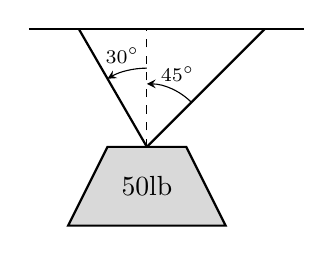
\begin{tikzpicture}
 \filldraw[thick,black,fill=gray!30] (-.5,0) -- (.5,0) -- (1,-1) -- (-1,-1)--cycle;
 \draw (0,-.5) node {50lb};
 \draw [thick] (-1.5,1.5) -- (2,1.5);
 \clip (-1.5,1.5) rectangle (2,-1.25);
 \draw [thick,rotate=120] (0,0) -- (3,0);
 \draw [thick,rotate=45] (0,0) -- (3,0);
 \draw [dashed] (0,0) -- (0,2);
 \draw [rotate=45,->,>=stealth] (.8,0) arc (0:45:.8);
 \draw [rotate=67] (1,0) node {\scriptsize $45^\circ$};
 \draw [rotate=90,->,>=stealth] (1,0) arc (0:30:1);
 \draw [rotate=105] (1.2,0) node {\scriptsize $30^\circ$};
\end{tikzpicture}}{ALT-TEXT-TO-BE-DETERMINED}}

% Example 11.6.2 and several similar examples and exercises need a short physics crash course:  forces are vectors and in particular add like vectors; an object is at rest iff all acting forces add up to the zero vector; force = mass times acceleration; the force of gravity near the surface of the earth is such that the acceleration of every object is 9.8 m/s^2.
\begin{example}[Finding Component Forces]\label{ex_vect6}
Consider a weight of 50lb hanging from two chains, as shown in \autoref{fig:vect6}. One chain makes an angle of $30^\circ$ with the vertical, and the other an angle of $45^\circ$. Find the force applied to each chain.
\solution
Knowing that gravity is pulling the 50lb weight straight down, we can create a vector $\vec F$ to represent this force. 
\[\vec F = 50\bracket{0,-1}=\bracket{0,-50}.\]

We can view each chain as ``pulling'' the weight up, preventing it from falling. We can represent the force from each chain with a vector. Let $\vec F_1$ represent the force from the chain making an angle of $30^\circ$ with the vertical, and let $\vec F_2$ represent the force form the other chain. Convert all angles to be measured from the horizontal (as shown in \autoref{fig:vect6b}), and apply \autoref{idea:unit_vectors}. As we do not yet know the magnitudes of these vectors, (that is the problem at hand), we use $m_1$ and $m_2$ to represent them.
\begin{align*}
\vec F_1 &= m_1\bracket{\cos 120^\circ,\sin120^\circ} \\
\vec F_2 &= m_2\bracket{\cos 45^\circ,\sin45^\circ}
\end{align*}
As the weight is not moving, we know the sum of the forces is $\vec 0$. This gives:
\begin{align*}
\vec F + \vec F_1 + \vec F_2 & = \vec 0\\
\bracket{0,-50}+ m_1\bracket{\cos 120^\circ,\sin120^\circ}+ m_2\bracket{\cos 45^\circ,\sin45^\circ}&=\vec 0
\end{align*}

\mtable{A diagram of the force vectors from \autoref{ex_vect6}.}{fig:vect6b}{\pdftooltip{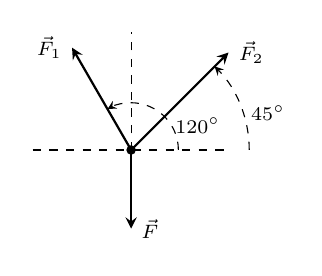
\begin{tikzpicture}[>=stealth]
 \draw [thick,rotate=120,->] (0,0) -- (1.5,0) node [left] {\scriptsize $\vec F_1$};
 \draw [thick,rotate=45,->] (0,0) -- (1.75,0)node [right] {\scriptsize $\vec F_2$};
 \draw [thick,rotate=-90,->] (0,0) -- (1,0) node [right] {\scriptsize $\vec F$};
 \draw [dashed] (0,0) -- (0,1.5);
 \draw [dashed] (-1.25,0) -- (1.25,0);
 \filldraw [black] (0,0) circle (1.5pt);
 \draw [dashed,->,>=stealth] (.6,0) arc (0:120:.6);
 \draw [rotate=20] (.9,0) node {\scriptsize $120^\circ$};
 \draw [dashed,->,>=stealth] (1.5,0) arc (0:45:1.5);
 \draw [rotate=15] (1.8,0) node {\scriptsize $45^\circ$};
\end{tikzpicture}}{ALT-TEXT-TO-BE-DETERMINED}}

The sum of the entries in the first component is 0, and the sum of the entries in the second component is also 0. This leads us to the following two equations:
\begin{align*}
m_1\cos120^\circ + m_2\cos45^\circ &=0 \\
m_1\sin120^\circ + m_2\sin45^\circ &=50
\end{align*}
This is a simple 2-equation, 2-unknown system of linear equations. We leave it to the reader to verify that the solution is 
\[
m_1=50(\sqrt{3}-1)\text{lb}% \approx 36.6
;\qquad
m_2=\frac{50\sqrt{2}}{1+\sqrt{3}}\text{lb}.% \approx 25.88.
\]

It might seem odd that the sum of the forces applied to the chains is more than 50lb. We leave it to a physics class to discuss the full details, but offer this short explanation. Our equations were established so that the \emph{vertical} components of each force sums to 50lb, thus supporting the weight. Since the chains are at an angle, they also pull against each other, creating an ``additional'' horizontal force while holding the weight in place.
\end{example}

Unit vectors were very important in the previous calculation; they allowed us to define a vector in the proper direction but with an unknown magnitude. Our computations were then computed component-wise. Because such calculations are often necessary, the \emph{standard unit vectors} can be useful.

\begin{definition}[Standard Unit Vectors]\label{def:standard_unit}
\index{vectors!standard unit vector}\index{unit vector!standard unit vector}%
\mbox{}\\[-2\baselineskip]\parbox[t]{\linewidth}{\begin{enumerate}
	\item In $\mathbb{R}^2$, the standard unit vectors are
	\[\veci =\bracket{1,0}\quad \text{and}\quad \vecj =\bracket{0,1}.\]
	\item In $\mathbb{R}^3$, the standard unit vectors are
	\[\veci =\bracket{1,0,0}\quad \text{and}\quad \vecj =\bracket{0,1,0}\quad \text{and}\quad \vec k =\bracket{0,0,1}.\]
\end{enumerate}}
\end{definition}

\begin{example}[Using standard unit vectors]\label{ex_vect7}
\mbox{}\\[-2\baselineskip]\parbox[t]{\linewidth}{%
\begin{enumerate}
	\item Rewrite $\vec v =\bracket{2,-3}$ using the standard unit vectors.
	\item	Rewrite $\vec w = 4\veci - 5\vecj +2\vec k$ in component form.
\end{enumerate}}\vspace{0pt}
\solution
\begin{enumerate}
	\item  \hfill$\begin{aligned}[t]
		\vec v &=\bracket{2,-3}\\
		&=\bracket{2,0}+\bracket{0,-3}\\
		&= 2\bracket{1,0}-3\bracket{0,1}\\
		&= 2\veci - 3\vecj
	\end{aligned}$\hfill\null
	
	\item	\hfill$\begin{aligned}[t]
		\vec w &= 4\veci - 5\vecj +2\vec k\\
		&=\bracket{4,0,0}+\bracket{0,-5,0}+\bracket{0,0,2}\\
		&=\bracket{4,-5,2}
	\end{aligned}$\hfill\null
\end{enumerate}
These two examples demonstrate that converting between component form and the standard unit vectors is rather straightforward. Many mathematicians prefer component form, and it is the preferred notation in this text. Many engineers prefer using the standard unit vectors, and many engineering texts use that notation.
\end{example}

\begin{example}[Finding Component Force]\label{ex_vect8}
A
%
\mtable{A figure of a weight being pushed by the wind in \autoref{ex_vect8}.}{fig:vect8}{\pdftooltip{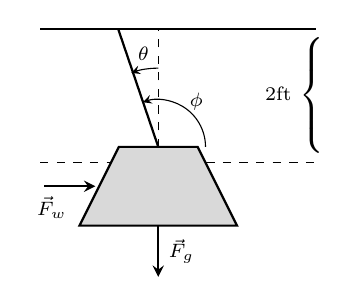
\begin{tikzpicture}
 \draw [dashed] (-1.5,-.2) -- (2,-.2);
 \draw (1.75,.65) node {\scriptsize 2ft $\left\{\rule{0pt}{.8cm}\right.$};
 \filldraw[thick,black,fill=gray!30] (-.5,0) -- (.5,0) -- (1,-1) -- (-1,-1)--cycle;
 \draw [thick] (-1.5,1.5) -- (2,1.5);
 \draw [thick] (0,0) -- (-.51,1.5); % diagonal line ~ 110 degrees
 \draw [dashed] (0,0) -- (0,1.5);
 \draw [rotate=90,->,>=stealth] (1,0) arc (0:20:1);
 %
 \draw [->,>=stealth] (.6,0) arc (0:109:.6);
 \draw [rotate=50] (.75,0) node {\scriptsize $\phi$};
 %
 \draw [rotate=99] (1.2,0) node {\scriptsize $\theta$};
 \draw [thick,->,>=stealth] (-1.45,-.5) -- (-.8,-.5) node [pos=.15,below] {\scriptsize $\vec F_w$};
 \draw [thick,->,>=stealth] (0,-1) -- (0,-1.65) node [pos=.5,right] {\scriptsize $\vec F_g$};
\end{tikzpicture}}{ALT-TEXT-TO-BE-DETERMINED}}
%
weight of 25lb is suspended from a chain of length 2ft while a wind pushes the weight to the right with constant force of 5lb as shown in \autoref{fig:vect8}. What angle will the chain make with the vertical as a result of the wind's pushing? How much higher will the weight be?
\solution
The force of the wind is represented by the vector $\vec F_w = 5\veci$. The force of gravity on the weight is represented by $\vec F_g = -25\vecj$. The direction and magnitude of the vector representing the force on the chain are both unknown. We represent this force with
\[\vec F_c = m\bracket{\cos\phi,\sin\phi}= m\cos\phi\, \veci + m\sin\phi\,\vecj\]
for some magnitude $m$ and some angle with the horizontal $\phi$. (Note: $\theta$ is the angle the chain makes with the \emph{vertical}; $\phi$ is the angle with the \emph{horizontal}.)

As the weight is at equilibrium, the sum of the forces is $\vec0$:
\begin{align*}
\vec F_c + \vec F_w + \vec F_g &= \vec 0\\
m\cos\phi\, \veci + m\sin\phi\,\vecj + 5\veci - 25\vecj &=\vec 0
\end{align*}

Thus the sum of the $\veci$ and $\vecj$ components are 0, leading us to the following system of equations:
\begin{align}
5+m\cos\phi &= 0\\
-25+m\sin\phi &= 0
\label{eq:vect8}
\end{align}

This is enough to determine $\vec F_c$ already, as we know $m\cos \phi = -5$ and $m\sin\phi =25$. Thus $F_c =\bracket{-5,25}.$ We can use this to find the magnitude $m$:
\[m = \sqrt{(-5)^2+25^2} = 5\sqrt{26}%\approx 25.5
\text{lb}.\]
We can then use either equality from \autoeqref{eq:vect8} to solve for $\phi$. We choose the first equality as using arccosine will return an angle in the $2^\text{nd}$ quadrant:
\[5 + 5\sqrt{26}\cos \phi = 0 \quad \Rightarrow \quad \phi = \cos^{-1}\left(\frac{-5}{5\sqrt{26}}\right) \approx 1.7682\approx 101.31^\circ.\]

Subtracting $90^\circ$ from this angle gives us an angle of $11.31^\circ$ with the vertical.

We can now use trigonometry to find out how high the weight is lifted. \autoref{fig:vect8} shows that a right triangle is formed with the 2ft chain as the hypotenuse.  We have found that the interior angle is $11.31^\circ$. The length of the adjacent side (in the diagram, the dashed vertical line) is $2\cos 11.31^\circ \approx 1.96$ft. Thus the weight is lifted by about $0.04$ft, almost 1/2in.
\end{example}

The algebra we have applied to vectors is already demonstrating itself to be very useful. There are two more fundamental operations we can perform with vectors, the \emph{dot product} and the \emph{cross product}. The next two sections explore each in turn.

\printexercises{exercises/10-02-exercises}

\section{The Dot Product}\label{sec:dot_product}

The previous section introduced vectors and described how to add them together and how to multiply them by scalars. This section introduces \emph{a} multiplication on vectors called the \textbf{dot product}.

\begin{definition}[Dot Product]\label{def:dot_product}%
\index{dot product!definition}\index{vectors!dot product}
\mbox{}\\[-2\baselineskip]\parbox[t]{\linewidth}{\begin{enumerate}
	\item Let $\vec u =\bracket{u_1,u_2}$ and $\vec v = \bracket{v_1,v_2}$  in $\mathbb{R}^2$. The \textbf{dot product} of $\vec u$ and $\vec v$, denoted $\vec u\cdot\vec v$, is 
	\[\vec u\cdot\vec v = u_1v_1+u_2v_2.\]
	\item Let $\vec u = \bracket{u_1,u_2,u_3}$ and $\vec v = \bracket{v_1,v_2,v_3}$  in $\mathbb{R}^3$. The \textbf{dot product} of $\vec u$ and $\vec v$, denoted $\vec u\cdot \vec v$, is 
	\[\vec u\cdot\vec v = u_1v_1+u_2v_2+u_3v_3.\]
\end{enumerate}}
\end{definition}

Note how this product of vectors returns a \emph{scalar}, not another vector.

We practice evaluating a dot product in the following example, then we will discuss why this product is useful.

\begin{example}[Evaluating dot products]\label{ex_dotp1}%
\mbox{}\\[-2\baselineskip]\parbox[t]{\linewidth}{%
\begin{enumerate}
	\item Let $\vec u=\bracket{1,2}$, $\vec v=\bracket{3,-1}$ in $\mathbb{R}^2$. Find $\vec u\cdot\vec v$.
	\item Let $\vec x = \bracket{2,-2,5}$ and $\vec y = \bracket{-1, 0, 3}$ in $\mathbb{R}^3$. Find $\vec x\cdot\vec y$.
\end{enumerate}}\vspace{0pt}
\solution
\begin{enumerate}
	\item Using \autoref{def:dot_product}, we have
	\[\vec u\cdot\vec v = 1(3)+2(-1) = 1.\]
	\item	Using the definition, we have
	\[\vec x\cdot\vec y = 2(-1)  -2(0) + 5(3) = 13.\]
\end{enumerate}
\end{example}

The dot product, as shown by the preceding example, is very simple to evaluate. It is only the sum of products. While the definition gives no hint as to why we would care about this operation, there is an amazing connection between the dot product and angles formed by the vectors. Before stating this connection, we give a theorem stating some of the properties of the dot product.

\begin{theorem}[Properties of the Dot Product]\label{thm:dot_product_properties}%
Let $\vec u$, $\vec v$ and $\vec w$ be vectors in $\mathbb{R}^2$ or $\mathbb{R}^3$ and let $c$ be a scalar.\index{dot product!properties}\index{vectors!dot product}
\begin{enumerate}
	\item \parbox{150pt}{$\vec u\cdot\vec v = \vec v\cdot\vec u$}{Commutative Property}
	\item \parbox{150pt}{$\vec u\cdot(\vec v+\vec w) = \vec u\cdot\vec v + \vec u\cdot\vec w$}{Distributive Property}
	\item	$c(\vec u\cdot\vec v) = (c\vec u)\cdot \vec v = \vec u \cdot (c\vec v)$
	\item	$\vec 0\cdot\vec v = 0$
	\item	$\vec v\cdot\vec v=\norm{\vec v}^2 $
\end{enumerate}
\end{theorem}

The last statement of the theorem makes a handy connection between the magnitude of a vector and the dot product with itself. Our definition and theorem give properties of the dot product, but we are still likely wondering ``What does the dot product \emph{mean}?'' It is helpful to understand that the dot product of a vector with itself is connected to its magnitude.

The next theorem extends this understanding by connecting the dot product to magnitudes and angles. Given vectors $\vec u$ and $\vec v$ in the plane, an angle $\theta$ is clearly formed when $\vec u$ and $\vec v$ are drawn with the same initial point as illustrated in \autoref{fig:dotpangle}(a). (We always take $\theta$ to be the angle in $[0,\pi]$ as two angles are actually created.) 

\mtable{Illustrating the angle formed by two vectors with the same initial point.}{fig:dotpangle}{%
\begin{tikzpicture}[alt={Vectors u, v share a tail; interior angle θ is sketched between the two arrow shafts.},>=stealth,scale=1.25]
	\draw [rotate=-15,->] (0,0) -- (2,0) node (A) [right] {\scriptsize $\vec u$};
	\draw [rotate=35,->] (0,0) -- (2.5,0) node (B) [right] {\scriptsize $\vec v$};
	\draw [rotate=-15,->] (.75,0) arc (0:50:.75);
	\draw [rotate=10] (.9,0) node {\scriptsize $\theta$};
\end{tikzpicture}
\\(a)\\[15pt]
\myincludeasythree{
3Droll=0,
3Dortho=0.0045,
3Dc2c=.54 .61 .58,
3Dcoo=0 0 40,
3Droo=170}{\marginparwidth}{3-D axes; u, v lie in a shaded plane through origin; angle θ marked between them.}{figures/figdotpangle3D_3D}
\\(b)}

The same is also true of 2 vectors in space: given $\vec u$ and $\vec v$ in $\mathbb{R}^3$ with the same initial point, there is a plane that contains both $\vec u$ and $\vec v$. (When $\vec u$ and $\vec v$ are co-linear, there are infinite planes that contain both vectors.) In that plane, we can again find an angle $\theta$ between them (and again, $0\leq \theta\leq \pi$). This is illustrated in \autoref{fig:dotpangle}(b).

The following theorem connects this angle $\theta$ to the dot product of $\vec u$ and $\vec v$.

\begin{theorem}[The Dot Product and Angles]\label{thm:dot_product}%
Let $\vec u$ and $\vec v$ be vectors in $\mathbb{R}^2$ or $\mathbb{R}^3$. Then 
\[\vec u\cdot\vec v = \norm{\vec u}\,\norm{\vec v} \cos\theta,\]
where $\theta$, $0\leq\theta\leq \pi$, is the angle between $\vec u$ and $\vec v$.
\index{dot product!properties}\index{vectors!dot product}
\end{theorem}

When $\theta$ is an acute angle (i.e., $0\leq \theta <\pi/2$), $\cos \theta$ is positive; when $\theta = \pi/2$, $\cos \theta = 0$; when $\theta$ is an obtuse angle ($\pi/2<\theta \leq \pi$), $\cos \theta$ is negative. Thus the sign of the dot product gives a general indication of the angle between the vectors, illustrated in \autoref{fig:dotpsign}.

\noindent\begin{minipage}[t]{\linewidth}\noindent%
\captionsetup{type=figure}%
\centering
\begin{tikzpicture}[alt={Panels: (1) acute θ between u and v, u·v > 0; (2) right angle θ = π⁄2, u·v = 0; (3) obtuse θ, u·v < 0.},>=stealth,thick,scale=1.25]
	\begin{scope}
		\draw[->] (0,0) -- (1,0) node [pos=.5,below]
		 {\scriptsize $\vec u\cdot \vec v >0$} node [right] {\scriptsize $\vec u$};
		\draw[->] (0,0) -- (.5,.866)node [above right] {\scriptsize $\vec v$};
		\draw[->] (.3,0) arc (0:60:.3);
		\draw[rotate=30] (.45,0) node {\scriptsize $\theta$};
	\end{scope}
	\begin{scope}[shift={(2.4cm,0)}]
		\draw[->] (0,0) -- (1,0)node [pos=.5,below]
		 {\scriptsize $\vec u\cdot \vec v =0$}node [right] {\scriptsize $\vec u$};
		\draw[->] (0,0) -- (0,1)node [above ] {\scriptsize $\vec v$};
		\draw[->] (.3,0) arc (0:90:.3);
		\draw[rotate=22.5] (.7,0) node {\scriptsize $\theta=\pi/2$};
	\end{scope}
	\begin{scope}[shift={(5.2cm,0)}]
		\draw[->] (0,0) -- (1,0)node [pos=.5,below]
		 {\scriptsize $\vec u\cdot \vec v <0$}node [right] {\scriptsize $\vec u$};
		\draw[->] (0,0) -- (-.707,.707)node [above left] {\scriptsize $\vec v$};
		\draw[->] (.3,0) arc (0:135:.3);
		\draw[rotate=67.5] (.45,0) node {\scriptsize $\theta$};
	\end{scope}
\end{tikzpicture}
\caption{Illustrating the relationship between the angle between vectors and the sign of their dot product.}
\label{fig:dotpsign}
\end{minipage}

We \emph{can} use \autoref{thm:dot_product} to compute the dot product, but generally this theorem is used to find the angle between known vectors (since the dot product is generally easy to compute). To this end, we rewrite the theorem's equation as\vspace{-.3\baselineskip}
\[\cos \theta = \frac{\vec u\cdot\vec v}{\norm{\vec u}\norm{\vec v}} \quad \Leftrightarrow \quad \theta = \cos^{-1}\left(\frac{\vec u\cdot\vec v}{\norm{\vec u}\norm{\vec v}}\right).\]

\youtubeVideo{98C7iv8OcnI}{Vectors: The Dot Product}

We practice using this theorem in the following example.

\mtable{Vectors used in \autoref{ex_dotp2}.}{fig:dotp2}{\begin{tikzpicture}[alt={On xy grid, rays u(3,1), v(–2,6), w(–4,3); arcs label alpha, beta, theta between the directions.},>=stealth]
\begin{axis}[width=1.16\marginparwidth,tick label style={font=\scriptsize},
axis y line=middle,axis x line=middle,name=myplot,axis on top,minor x tick num=4,
minor y tick num=1,ymin=-1.8,ymax=6.99,xmin=-5.5,xmax=5.5]
\draw [thick,->] (axis cs:0,0) --(axis cs: 3,1) node [above] {\scriptsize$\vec u$};
\draw [thick,->] (axis cs:0,0) --(axis cs: -2,6) node [above] {\scriptsize$\vec v$};
\draw [thick,->] (axis cs:0,0) --(axis cs: -4,3) node [above] {\scriptsize$\vec w$};
\draw [->] (axis cs: .949,.316) arc (18.4:108.4:12pt);
\draw [] (axis cs:0.680986, 1.33651) node {\scriptsize $\alpha$};
\draw [->] (axis cs: -0.474342, 1.42302) arc (108.4:155.1:12pt);
\draw [] (axis cs:-1.13929, 1.58257) node {\scriptsize $\beta$};
\draw [->] (axis cs: 2.3725, 0.79) arc (18.4:143.1:30pt);
\draw [] (axis cs:1.5, 2.59808) node {\scriptsize $\theta$};
\end{axis}
\node [right] at (myplot.right of origin) {\scriptsize $x$};
\node [above] at (myplot.above origin) {\scriptsize $y$};
\end{tikzpicture}}

\begin{example}[Using the dot product to find angles]\label{ex_dotp2}%
Let $\vec u = \bracket{3,1}$, $\vec v = \bracket{-2,6}$ and $\vec w = \bracket{-4,3}$, as shown in \autoref{fig:dotp2}. Find the angles $\alpha$, $\beta$ and $\theta$.
\solution
We start by computing the magnitude of each vector.
\[
\norm{\vec u} = \sqrt{10};\quad \norm{\vec v} = 2\sqrt{10};\quad \norm{\vec w} = 5.
\]
We now apply \autoref{thm:dot_product} to find the angles.
\begin{align*}
	\alpha &= \cos^{-1}\left(\frac{\vec u\cdot\vec v}{(\sqrt{10})(2\sqrt{10})}\right) \\
	&= \cos^{-1}(0) = \frac{\pi}2 = 90^\circ.\displaybreak[0]\\[10pt]
	\beta &= \cos^{-1}\left(\frac{\vec v\cdot\vec w}{(2\sqrt{10})(5)}\right) \\
	&= \cos^{-1}\left(\frac{26}{10\sqrt{10}}\right) \\
	&\approx 0.6055 \approx 34.7^\circ.\displaybreak[0]\\[10pt]
	\theta &= \cos^{-1}\left(\frac{\vec u\cdot\vec w}{(\sqrt{10})(5)}\right) \\
	&= \cos^{-1}\left(\frac{-9}{5\sqrt{10}}\right) \\
	&\approx 2.1763 \approx 124.7^\circ
\end{align*}
\end{example}

We see from our computation that $\alpha + \beta = \theta$, as indicated by \autoref{fig:dotp2}. While we knew this should be the case, it is nice to see that this non-intuitive formula indeed returns the results we expected.

We do a similar example next in the context of vectors in space.

\mtable{Vectors used in \autoref{ex_dotp3}.}{fig:dotp3}{%
\myincludeasythree{
3Droll=0,
3Dortho=0.0045,
3Dc2c=.89 .4 .23,
3Dcoo=10 50 46,
3Droo=200}{\marginparwidth}{Axes in space with u(3,1,0), v(2,–5,–3), w(–1,4,4); dashed boxes show xyz components.}{figures/figdotp3_3D}}

\begin{example}[Using the dot product to find angles]\label{ex_dotp3}%
Let $\vec u = \bracket{1,1,1}$, $\vec v = \bracket{-1,3,-2}$ and $\vec w = \bracket{-5,1,4}$, as illustrated in \autoref{fig:dotp3}. Find the angle between each pair of vectors.
\solution
\begin{enumerate}
	\item Between $\vec u$ and $\vec v$:\vspace{-\baselineskip}
	\begin{align*}
		\theta &= \cos^{-1}\left(\frac{\vec u\cdot\vec v}{\norm{\vec u}\norm{\vec v}}\right)\\
		&= \cos^{-1}\left(\frac{0}{\sqrt{3}\sqrt{14}}\right)\\
		&= \frac{\pi}2.
	\end{align*}
	\item	Between $\vec u$ and $\vec w$:\vspace{-\baselineskip}
	\begin{align*}
		\theta &= \cos^{-1}\left(\frac{\vec u\cdot\vec w}{\norm{\vec u}\norm{\vec w}}\right)\\
		&= \cos^{-1}\left(\frac{0}{\sqrt{3}\sqrt{42}}\right)\\
		&= \frac{\pi}2.
	\end{align*}
	\item	Between $\vec v$ and $\vec w$:\vspace{-\baselineskip}
	\begin{align*}
		\theta &= \cos^{-1}\left(\frac{\vec v\cdot\vec w}{\norm{\vec v}\norm{\vec w}}\right)\\
		&= \cos^{-1}\left(\frac{0}{\sqrt{14}\sqrt{42}}\right)\\
		&= \frac{\pi}2.
	\end{align*}
\end{enumerate}
While our work shows that each angle is $\pi/2$, i.e.,  $90^\circ$, none of these angles looks to be a right angle in \autoref{fig:dotp3}. Such is the case when drawing three-dimensional objects on the page.
\end{example}

All three angles between these vectors was $\pi/2$, or $90^\circ$. We know from geometry and everyday life that $90^\circ$ angles are ``nice'' for a variety of reasons, so it should seem significant that these angles are all $\pi/2$. Notice the common feature in each calculation (and also the calculation of $\alpha$ in \autoref{ex_dotp2}): the dot products of each pair of angles was 0. We use this as a basis for a definition of the term \textbf{orthogonal}, which is essentially synonymous to \emph{perpendicular}.

\begin{definition}[Orthogonal]\label{def:orthogonal}%
Vectors $\vec u$ and $\vec v$ are \textbf{orthogonal} if their dot product is 0.
\index{orthogonal}\index{vectors!orthogonal}
\end{definition}

\mnote{\textbf{Note:} The term \emph{perpendicular} originally referred to lines. As mathematics progressed, the concept of ``being at right angles to'' was applied to other objects, such as vectors and planes, and the term \emph{orthogonal} was introduced. It is especially used when discussing objects that are hard, or impossible, to visualize: two vectors in 5-dimensional space are orthogonal if their dot product is 0. It is not wrong to say they are \emph{perpendicular}, but common convention gives preference to the word \emph{orthogonal}.}

\begin{example}[Finding orthogonal vectors]\label{ex_dotp8}%
Let $\vec u = \bracket{3,5}$ and $\vec v = \bracket{1,2,3}$. 
\begin{enumerate}
	\item Find two vectors in $\mathbb{R}^2$ that are orthogonal to $\vec u$.
	\item	Find two non-parallel vectors in $\mathbb{R}^3$ that are orthogonal to $\vec v$.
\end{enumerate}
\solution
\begin{enumerate}
	\item Recall that a line perpendicular to a line with slope $m$ has slope $-1/m$, the ``opposite reciprocal slope.'' We can think of the slope of $\vec u$ as $5/3$, its ``rise over run.'' A vector orthogonal to $\vec u$ will have slope $-3/5$. There are many such choices, though all parallel:
	\[\bracket{-5,3}\quad \text{or} \quad\bracket{5,-3}\quad \text{or} \quad \bracket{-10,6}\quad \text{or} \quad \bracket{15,-9},\text{etc.}\]
	\item		There are infinite directions in space orthogonal to any given direction, so there are an infinite number of non-parallel vectors orthogonal to $\vec v$. Since there are so many, we have great leeway in finding some.
	
	One way is to arbitrarily pick values for the first two components, leaving the third unknown. For instance, let $\vec v_1 = \bracket{2,7,z}$. If $\vec v_1$ is to be orthogonal to $\vec v$, then $\vec v_1\cdot\vec v = 0$, so 
	\[2+14+3z=0 \quad \Rightarrow \quad z = \frac{-16}{3}.\]
	So $\vec v_1 = \bracket{2, 7, -16/3}$ is orthogonal to $\vec v$. We can apply a similar technique by leaving the first or second component unknown.
	
	Another method of finding a vector orthogonal to $\vec v$ mirrors what we did in part 1. Let $\vec v_2 = \bracket{-2,1,0}$. Here we switched the first two components of $\vec v$, changing the sign of one of them (similar to the ``opposite reciprocal'' concept before). Letting the third component be 0 effectively ignores the third component of $\vec v$, and it is easy to see that 
	\[\vec v_2\cdot\vec v = \bracket{-2,1,0}\cdot\bracket{1,2,3}= 0.\]
	Clearly $\vec v_1$ and $\vec v_2$ are not parallel.
\end{enumerate}
\end{example}

\mtable{Developing the construction of the \emph{orthogonal projection}.}{fig:dotpproj}{%
\begin{tikzpicture}[alt={Triangle from origin: u to apex, dashed height meets v at right angle to build projection.},>=stealth]
	\draw [thick,->] (0,0) -- (4,2) node [right] {\scriptsize $\vec v$};
	\draw [thick,->] (0,0) -- (1,3) node [above ] {\scriptsize $\vec u$};
	\draw [dotted,thick] (1,3) -- (2,1);
	\draw (1.82111, 0.910557) -- ({1.73167, 1.08944})--(1.91056, 1.17889);
	\draw (.4,.2) arc (26.5:71.6:.45);
	\draw [rotate=49] (.6,0) node {\scriptsize $\theta$};
\end{tikzpicture}
\\(a)\\[15pt]
\begin{tikzpicture}[alt={Triangle from origin: height labelled z, foot labelled w; grey v emphasises projection line.},>=stealth]
	\draw [thick,->] (2,1) -- (4,2) node [right] {\scriptsize $\vec v$};
	\draw [thick,->] (0,0) -- (1,3) node [above ] {\scriptsize $\vec u$};
	\draw [thick,->,gray] (0,0) -- (2,1) node [below,black] {\scriptsize $\vec w$};
	\draw [<-,thick] (1,3) -- (2,1) node [right,pos=.5] {\scriptsize $\vec z$};
	\draw (1.82111, 0.910557) -- ({1.73167, 1.08944})--(1.91056, 1.17889);
	\draw (.4,.2) arc (26.5:71.6:.45);
	\draw [rotate=49] (.6,0) node {\scriptsize $\theta$};
\end{tikzpicture}
\\(b)}

An important construction is illustrated in \autoref{fig:dotpproj}, where vectors $\vec u$ and $\vec v$ are sketched. In part (a), a dotted line is drawn from the tip of $\vec u$ to the line containing $\vec v$, where the dotted line is orthogonal to $\vec v$. In part (b), the dotted line is replaced with the vector $\vec z$ and  $\vec w$ is formed, parallel to $\vec v$. It is clear by the diagram that $\vec u = \vec w+\vec z$. What is important about this construction is this: $\vec u$ is \emph{decomposed} as the sum of two vectors, one of which is parallel to $\vec v$ and one that is perpendicular to $\vec v$. It is hard to overstate the importance of this construction (as we'll see in upcoming examples). 

The vectors $\vec w$, $\vec z$ and $\vec u$ as shown in \autoref{fig:dotpproj} (b) form a right triangle, where the angle between $\vec v$ and $\vec u$ is labeled $\theta$. We can find $\vec w$ in terms of $\vec v$ and $\vec u$.

Using trigonometry, we can state that 
\begin{equation}
\norm{\vec w} = \norm{\vec u}\cos \theta. \label{eq:proj1}%
\end{equation}

We also know that $\vec w$ is parallel to to $\vec v$\,; that is, the direction of $\vec w$ is the direction of $\vec v$, described by the unit vector $\frac{1}{\norm{\vec v}}\vec v$. The vector $\vec w$ is the vector in the direction $\frac{1}{\norm{\vec v}}\vec v$ with magnitude $\norm{\vec u}\cos \theta$:
\begin{align*}
\vec w &= \Bigl(\norm{\vec u}\cos\theta \Bigr)\frac{1}{\norm{\vec v}}\vec v.
\intertext{Replace $\cos\theta$ using \autoref{thm:dot_product}:}
			&= \left(\norm{\vec u}\frac{\vec u\cdot\vec v}{\norm{\vec u}\norm{\vec v}}\right)\frac{1}{\norm{\vec v}} \vec v\\ 
			&= \frac{\vec u\cdot\vec v}{\norm{\vec v}^2}\vec v.
			\intertext{Now apply \autoref{thm:dot_product_properties}.}
			&= \frac{\vec u\cdot\vec v}{\vec v\cdot\vec v}\vec v.
\end{align*}

Since this construction is so important, it is given a special name.

\begin{definition}[Orthogonal Projection]\label{def:orthogonal_projection}%
Let $\vec u$ and $\vec v$ be given, where $\vec v\neq\vec 0$. The \textbf{orthogonal projection of $\vec u$ onto $\vec v$}, denoted $\proj uv$, is 
\index{orthogonal projection}\index{vectors!orthogonal projection}
\[\proj uv = \frac{\vec u\cdot\vec v}{\vec v\cdot\vec v}\vec v.\]
\end{definition}

\mtable[-1in]{Graphing the vectors used in \autoref{ex_dotp4}.}{fig:dotp4}{%
\begin{tikzpicture}[alt={2-D plot of u, v and proj_v; right-angle tick at foot; axes graduated.},>=stealth]
\begin{axis}[width=1.16\marginparwidth,tick label style={font=\scriptsize},
axis y line=middle,axis x line=middle,name=myplot,axis on top,xtick={-3,-2,-1,1,2,3},
ytick={1,2,-1,-2},ymin=-2.8,ymax=2.8,xmin=-2.9,xmax=3.9]
\draw [thick,->] (axis cs:0,0) --(axis cs: -2,1) node [above] {\scriptsize$\vec u$};
\draw [thick,->] (axis cs:0,0) --(axis cs: 3,1) node [above] {\scriptsize$\vec v$};
\draw [thick,->,gray] (axis cs:0,0) --(axis cs: -1.5,-.5)
 node [below,black] {\scriptsize$\text{proj}_{\, \vec v}\, \vec u$};
\draw [dotted,thick] (axis cs: -2,1) -- (axis cs:-1.5,-.5);
\end{axis}
\node [right] at (myplot.right of origin) {\scriptsize $x$};
\node [above] at (myplot.above origin) {\scriptsize $y$};
\end{tikzpicture}
\\(a)\\[15pt]
\myincludeasythree{
3Droll=0,
3Dortho=0.0046,
3Dc2c=.9 .12 .42,
3Dcoo=0 50 30,
3Droo=250}{.8\marginparwidth}{3-D view: blue w, red proj_v w, black x; dashed cubes outline component lengths.}{figures/figdotp4b_3D}
\\(b)
\iftoggle{in_threeD}{}{%
\\[15pt]
\myincludegraphics[alt={3-D view: blue w, red proj_v w, black x; dashed cubes outline component lengths.},width=.8\marginparwidth]{figures/figdotp4c_3D} % myinc g 3D
\\(c)}% end iftoggle
}% end mtable

\begin{example}[Computing the orthogonal projection]\label{ex_dotp4}%
\mbox{}\\[-2\baselineskip]\parbox[t]{\linewidth}{%
\begin{enumerate}
	\item Let $\vec u=\bracket{-2,1}$ and $\vec v=\bracket{3,1}$. Find $\proj uv$, and sketch all three vectors with initial points at the origin.
	\item	Let $\vec w =\bracket{2,1,3}$ and $\vec x =\bracket{1,1,1}$. Find $\proj wx$, and sketch all three vectors with initial points at the origin.
\end{enumerate}}\vspace{0pt}
\solution
\begin{enumerate}
	\item Applying \autoref{def:orthogonal_projection}, we have
	\begin{align*}
		\proj uv
		&= \frac{\vec u\cdot\vec v}{\vec v\cdot\vec v}\vec v \\
		&= \frac{-5}{10}\bracket{3,1}\\
		&=\bracket{-\frac32,-\frac12}.
	\end{align*}
	Vectors $\vec u$, $\vec v$ and $\proj uv$ are sketched in \autoref{fig:dotp4}(a). Note how the projection is parallel to $\vec v$; that is, it lies on the same line through the origin as $\vec v$, although it points in the opposite direction. That is because the angle between $\vec u$ and $\vec v$ is obtuse (i.e., greater than $90^\circ$).
	
	\item	Apply the definition:
	\begin{align*}
		\proj wx
		&= \frac{\vec w\cdot\vec x}{\vec x\cdot\vec x}\vec x \\
		&= \frac{6}{3}\bracket{1,1,1}\\
		&=\bracket{2,2,2}.
	\end{align*}
	\iftoggle{in_threeD}{%
	 These vectors are sketched in \autoref{fig:dotp4}(b).%
	}
\end{example}

Consider \autoref{fig:dotpprojc} where the concept of the orthogonal projection is again illustrated. It is clear that
\begin{equation}
\vec u = \proj uv + \vec z.
\label{eq:orthogproj}
\end{equation}
As we know what $\vec u$ and $\proj uv$ are, we can solve for $\vec z$ and state that
\[\vec z = \vec u - \proj uv.\]%
%
\mtable[-7\baselineskip]{Illustrating the orthogonal projection.}{fig:dotpprojc}{\begin{tikzpicture}[alt={Vectors u, v with right-angle foot; z fills gap so u = proj_v u + z.},>=stealth]
 \draw [thick,->] (2,1) -- (4,2) node [below] {\scriptsize $\vec v$};
 \draw [thick,->] (0,0) -- (1,3) node [above ] {\scriptsize $\vec u$};
 \draw [thick,->,gray] (0,0) -- (2,1)
  node [pos=.6,below,black] {\scriptsize $\text{proj}_{\, \vec v}\, \vec u$};
 \draw [<-,thick] (1,3) -- (2,1) node [right,pos=.5] {\scriptsize $\vec z$};
 \draw (1.82111, 0.910557) -- ({1.73167, 1.08944})--(1.91056, 1.17889);
\end{tikzpicture}}%
%
This leads us to rewrite \autoeqref{eq:orthogproj} in a seemingly silly way:
\[\vec u = \proj uv + (\vec u - \proj uv).\]
This is not nonsense, as pointed out in the following Key Idea. (Notation note: the expression ``$\parallel \vec y$\,'' means ``is parallel to $\vec y$.'' We can use this notation to state ``$\vec x\parallel\vec y$\,'' which means ``$\vec x$ is parallel to $\vec y$.'' The expression ``$\perp \vec y$\,'' means ``is orthogonal to $\vec y$,'' and is used similarly.)

\begin{keyidea}[Orthogonal Decomposition of Vectors]\label{idea:orthog_proj}%
Let $\vec u$ and $\vec v$ be given. Then $\vec u$ can be written as the sum of two vectors, one of which is parallel to $\vec v$, and one of which is orthogonal to $\vec v$:
\index{orthogonal decomposition of vectors}\index{orthogonal!decomposition}\index{vectors!orthogonal decomposition}
\[\vec u = \underbrace{\proj uv}_{\parallel\ \vec v}\ +\  (\underbrace{\vec u-\proj uv}_{\perp\ \vec v}).\]
\end{keyidea}

We illustrate the use of this equality in the following example.

\begin{example}[Orthogonal decomposition of vectors]\label{ex_dotp5}%
\mbox{}\\[-2\baselineskip]\parbox[t]{\linewidth}{%
\begin{enumerate}
	\item Let $\vec u =\bracket{-2,1}$ and $\vec v =\bracket{3,1}$ as in \autoref{ex_dotp4}. Decompose $\vec u$ as the sum of a vector parallel to $\vec v$ and a vector orthogonal to $\vec v$.
	\item	Let $\vec w =\bracket{2,1,3}$ and $\vec x  =\bracket{1,1,1}$ as in \autoref{ex_dotp4}. Decompose $\vec w$ as the sum of a vector parallel to $\vec x$ and a vector orthogonal to $\vec x$.
\end{enumerate}}\vspace{0pt}
\solution
\begin{enumerate}
	\item In \autoref{ex_dotp4}, we found that $\proj uv =\bracket{-1.5,-0.5}$. Let
	\[\vec z = \vec u - \proj uv =\bracket{-2,1}-\bracket{-1.5,-0.5}=\bracket{-0.5, 1.5}.\]
	Is $\vec z$ orthogonal to $\vec v$\,? (I.e, is $\vec z \perp\vec v$\ ?) We check for orthogonality with the dot product:
	\[\vec z\cdot\vec v =\bracket{-0.5,1.5}\cdot\bracket{3,1}=0.\]
	Since the dot product is 0, we know $\vec z \perp \vec v$. Thus:
	\begin{align*}
	\vec u &= \proj uv\ +\ (\vec u - \proj uv) \\
	\bracket{-2,1}&= \underbrace{\bracket{-1.5,-0.5}}_{\parallel\ \vec v}\ +\ \underbrace{\bracket{-0.5,1.5}}_{\perp \ \vec v}.
	\end{align*}
	
	\item	We found in \autoref{ex_dotp4} that $\proj wx =\bracket{2,2,2}$. Applying the \autoref{idea:orthog_proj}, we have:
	\[\vec z = \vec w - \proj wx =\bracket{2,1,3}-\bracket{2,2,2}=\bracket{0,-1,1}.\] We check to see if $\vec z \perp \vec x$:
	\[\vec z\cdot\vec x =\bracket{0,-1,1}\cdot\bracket{1,1,1}= 0.\]
	Since the dot product is 0, we know the two vectors are orthogonal.
	We now write $\vec w$ as the sum of two vectors, one parallel and one orthogonal to $\vec x$:
	\begin{align*}
	\vec w &= \proj wx\ +\ (\vec w - \proj wx) \\
	\bracket{2,1,3}&= \underbrace{\bracket{2,2,2}}_{\parallel\ \vec x}\ +\ \underbrace{\bracket{0,-1,1}}_{\perp \ \vec x}
	\end{align*}
\end{enumerate}
\end{example}

We give an example of where this decomposition is useful.

\begin{example}[Orthogonally decomposing a force vector]\label{ex_dotp6}%
Consider \autoref{fig:dotp6}(a), showing a box weighing 50 lb on a ramp that rises 5 ft over a span of 20 ft. Find the components of force, and their magnitudes, acting on the box (as sketched in part (b) of the figure):
%
\mtable[-3\baselineskip]{Sketching the ramp and box in \autoref{ex_dotp6}. Note: \emph{The vectors are not drawn to scale.}}{fig:dotp6}{%
\begin{tikzpicture}[alt={20 by 5 ramp; weight g acts vertically on box resting on the incline.},>=stealth,scale=.2]
	\draw [thick,->] (20,5) -- node [right,pos=.5] {\scriptsize $5$} (20,0)
	 -- node [below,pos=.6] {\scriptsize 20}(0,0)
	 -- (20,5) node [above] {\scriptsize $\vec r$};
	\draw [thick] (10,2.5) -- (9.25,5.5) -- (12.25,6.25) -- (13,3.25);
	\draw [thick,->] (11.125,4.375) -- (11.125,-3.625)
	 node [below] {\scriptsize $\vec g$};
\end{tikzpicture}
\\(a)\\[15pt]
\begin{tikzpicture}[alt={20 by 5 ramp; g split into grey proj_r g along ramp plus orthogonal residual z.},>=stealth,scale=.2]
	\draw [thick,->] (20,5) -- node [right,pos=.5] {\scriptsize $5$} (20,0)
	 -- node [below,pos=.6] {\scriptsize 20}(0,0)
	 -- (20,5) node [above] {\scriptsize $\vec r$};
	\draw [thick] (10,2.5) -- (9.25,5.5) -- (12.25,6.25) -- (13,3.25);
	\draw [thick,->] (11.125,4.375) -- (11.125,-3.625)
	 node [below] {\scriptsize $\vec g$};
	\draw [gray,thick,->] (11.125,4.375) -- (13,-3.15)
	 node [right,pos=.4,black] {\scriptsize $\vec z$};
	\draw [gray,thick,->] (13,-3.15) -- (11.125,-3.625)
	 node [shift={(5pt,-5pt)} ,black,pos=0] {\scriptsize $\proj gr$};
\end{tikzpicture}
\\(b)}
%
\begin{enumerate}
	\item in the direction of the ramp, and
	\item	orthogonal to the ramp.
\end{enumerate}
\solution
As the ramp rises 5 ft over a horizontal distance of 20 ft, we can represent the direction of the ramp with the vector $\vec r=\bracket{20,5}$. Gravity pulls down with a force of 50 lb, which we represent with $\vec g =\bracket{0,-50}$. 
\begin{enumerate}
	\item To find the force of gravity in the direction of the ramp, we compute the projection $\proj gr$:\vspace{-.5\baselineskip}
	\begin{align*}
	\proj gr &= \frac{\vec g\cdot\vec r}{\vec r\cdot\vec r}\vec r\\
	&=  \frac{-250}{425}\bracket{20,5}\\
	&=\bracket{-\frac{200}{17},-\frac{50}{17}}%\approx\bracket{-11.76,-2.94}
	.
	\end{align*}
	The magnitude of $\proj gr$ is $\norm{\proj gr} = 50/\sqrt{17} \approx 12.13\text{ lb}$. Though the box weighs 50 lb, a force of about 12 lb is enough to keep the box from sliding down the ramp.
	
	\item		To find the component $\vec z$ of gravity orthogonal to the ramp, we use \autoref{idea:orthog_proj}.\vspace{-.5\baselineskip}
	\begin{align*}
	\vec z &= \vec g - \proj gr \\
	&=\bracket{\frac{200}{17},-\frac{800}{17}}%\approx\bracket{11.76,-47.06}
	.
	\end{align*}
	The magnitude of this force is $\norm{\vec z}=200/\sqrt{17}%\approx 48.51
	$ lb. In physics and engineering, knowing this force is important when computing things like static frictional force. (For instance, we could easily compute if the static frictional force alone was enough to keep the box from sliding down the ramp.)
\end{enumerate}
\end{example}

\subsection{Application to Work}

In physics, the application of a force $F$ to move an object in a straight line a distance $d$ produces \emph{work}; the amount of work $W$ is $W=Fd$, (where $F$ is in the direction of travel). The orthogonal projection allows us to compute work when the force is not in the direction of travel.

Consider \autoref{fig:dotpwork}, where a force $\vec F$ is being applied to an object moving in the direction of $\vec d$. (The distance the object travels is the magnitude of $\vec d$.) The work done is the amount of force in the direction of $\vec d$, $\norm{\proj Fd}$, times $\vnorm d$:

\mtable{Finding work when the force and direction of travel are given as vectors.}{fig:dotpwork}{\begin{tikzpicture}[alt={Box pulled by force F; horizontal travel d; grey proj_d F shows effective work.},>=stealth,scale=.8]
 \draw [thick] (0,0) rectangle (2,2);
 \draw [thick,->] (0,-.25) -- (5,-.25) node [right] {\scriptsize $\vec d$};
 \draw [thick,->] (1,1) -- (3,2) node [shift={(5pt,2.5pt)}] {\scriptsize $\vec F$};
 \draw [thick,gray,->] (1,1) -- (3,1) node [right,black] {\scriptsize $\proj Fd$};
\end{tikzpicture}}

\begin{align*}
\norm{\proj Fd}\cdot\vnorm d
 &= \norm{\frac{\vec F\cdot\vec d}{\vec d\cdot\vec d}\vec d}\cdot \vnorm d \\
		&= \abs{\frac{\vec F\cdot\vec d}{\vnorm d^2}}\cdot \vnorm d\cdot\vnorm d\\
		&= \frac{\abs{\vec F\cdot\vec d}}{\vnorm d^2}\vnorm d^2\\
		&= \abs{\vec F\cdot\vec d}.
\end{align*}

The expression $\vec F\cdot\vec d$ will be positive if the angle between $\vec F$ and $\vec d$ is acute; when the angle is obtuse (hence $\vec F\cdot\vec d$ is negative), the force is causing motion in the opposite direction of $\vec d$, resulting in ``negative work.'' We want to capture this sign, so we drop the absolute value and find that $W = \vec F\cdot\vec d$.

\begin{definition}[Work]\label{def:work}%
Let $\vec F$ be a constant force that moves an object in a straight line from point $P$ to point $Q$. Let $\vec d = \vv{PQ}$. The \textbf{work} $W$ done by $\vec F$ along $\vec d$ is $W = \vec F\cdot\vec d$.\index{work}
\end{definition}

\mtable{Computing work when sliding a box up a ramp in \autoref{ex_dotp7}.}{fig:dotp7}{\begin{tikzpicture}[alt={Force F 30 deg above ramp of rise 3 run 15; dashed component along slope marked.},>=stealth,scale=.3]
 \draw [thick] (0,0) -- node [below,pos=.5] {\scriptsize 15} (15,0)
  -- node [right, pos=.5] {\scriptsize 3} (15,3) -- cycle;
 \draw [thick] (5,1) -- (4.55,3.25) -- (6.8,3.7) -- (7.25,1.45);
 \begin{scope}[,shift={(5.9,2.35)}]
  \draw [thick,rotate=30,->] (0,0) -- (5,0) node [right] {\scriptsize $\vec F$};
  \draw [thick,dashed] (-2,0) -- (4,0);
  \draw (2,0) arc (0:30:2);
  \draw [rotate=15] (3,0) node {\scriptsize $30^\circ$};
 \end{scope}
\end{tikzpicture}}

\begin{example}[Computing work]\label{ex_dotp7}%
A man slides a box along a ramp that rises 3 ft over a distance of 15 ft by applying 50 lb of force as shown in \autoref{fig:dotp7}. Compute the work done.
\solution
The figure indicates that the force applied makes a $30^\circ$ angle with the horizontal, so $\vec F = 50\bracket{\cos 30^\circ,\sin 30^\circ}\bracket{25\sqrt3,25}%\approx\bracket{43.3,25}
$. The ramp is represented by $\vec d  =\bracket{15,3}$. The work done is simply
\[\vec F\cdot\vec d = \bracket{25\sqrt3,25}\cdot\bracket{15,3}=375\sqrt3+75%\approx 724.5
\text{ ft-lb}.\]

Note how we did not actually compute the distance the object traveled, nor the magnitude of the force in the direction of travel; this is all inherently computed by the dot product.
\end{example}

The dot product is a powerful way of evaluating computations that depend on angles without actually using angles. The next section explores another product on vectors, the \emph{cross product.} Once again, angles play an important role, though in a much different way.

\printexercises{exercises/10-03-exercises}

\section{The Cross Product}\label{sec:cross_product}

``Orthogonality'' is immensely important. A quick scan of your current environment will undoubtedly reveal numerous surfaces and edges that are perpendicular to each other (including the edges of this page). The dot product provides a quick test for orthogonality:  vectors $\vec u$ and $\vec v$ are perpendicular if, and only if, $\vec u\cdot\vec v=0$. 

Given two non-parallel, nonzero vectors $\vec u$ and $\vec v$ in space, it is very useful to find a vector $\vec w$ that is perpendicular to both $\vec u$ and $\vec v$. There is a operation, called the \textbf{cross product}, that creates such a vector. This section defines the cross product, then explores its properties and applications.

\definition{def:cross_product}{Cross Product}
{Let $\vec u =\bracket{u_1,u_2,u_3}$ and $\vec v = \bracket{v_1,v_2,v_3}$ be vectors in $\mathbb{R}^3$. The \textbf{cross product of $\vec u$ and $\vec v$}, denoted $\crossp uv$, is the vector
\index{vectors!cross product}\index{cross product!definition}
\[\crossp uv = \bracket{u_2v_3-u_3v_2,-(u_1v_3-u_3v_1),u_1v_2-u_2v_1}.\]}

This definition can be a bit cumbersome to remember. After an example we will give a convenient method for computing the cross product. For now, careful examination of the products and differences given in the definition should reveal a pattern that is not too difficult to remember. (For instance, in the first component only 2 and 3 appear as subscripts; in the second component, only 1 and 3 appear as subscripts. Further study reveals the order in which they appear.)

\youtubeVideo{qsgK1d-_8ik}{Cross Product}

Let's practice using this definition by computing a cross product.

\example{ex_crossp1}{Computing a cross product}{Let $\vec u = \bracket{2,-1,4}$ and $\vec v = \bracket{3,2,5}$. Find $\crossp uv$, and verify that it is orthogonal to both $\vec u$ and $\vec v$.}
{Using \autoref{def:cross_product}, we have
\[
\crossp uv = \bracket{(-1)5-(4)2,-\big((2)5-(4)3\big), (2)2-(-1)3}=\bracket{-13,2,7}.
\] 
(We encourage the reader to compute this product on their own, then verify their result.)

We test whether or not $\crossp uv$ is orthogonal to $\vec u$ and $\vec v$ using the dot product:
\begin{align*}
\big(\crossp uv\big) \cdot \vec u &=\bracket{-13,2,7}\cdot\bracket{2,-1,4}=0, \\
\big(\crossp uv\big) \cdot \vec v &=\bracket{-13,2,7}\cdot\bracket{3,2,5}=0.
\end{align*}
Since both dot products are zero, $\crossp uv$ is indeed orthogonal to both $\vec u$ and $\vec v$.}

\subsection{Additional Material on \texorpdfstring{$2\times2$ and $3\times3$}{2x2 and 3x3} determinants}

We will now make a slight digression.  Given four numbers $a$, $b$, $c$, $d$ we define the $2 \times 2$ determinant
\[\begin{vmatrix}a & b \\ c & d\end{vmatrix} = ad - bc.\]
Thus
\[
\begin{vmatrix}1 & 2 \\3 & 4\end{vmatrix} = -2
\text{ and }
\begin{vmatrix}3 & -2 \\-6 & 4\end{vmatrix} = 0.
\]

Given nine numbers $r_1$, $r_2$, $r_3$, $s_1$, $s_2$, $s_3$, $t_1$, $t_2$, $t_3$ we define the $3 \times 3$ determinant in terms of three $2 \times 2$ determinants as follows
\[
\begin{vmatrix}r_1 & r_2 & r_3 \\s_1 & s_2 & s_3 \\t_1 & t_2 & t_3\end{vmatrix} 
=
r_1 \begin{vmatrix}s_2 & s_3 \\t_2 & t_3\end{vmatrix}
\stackrel{!}{-}r_2 \begin{vmatrix}s_1 & s_3 \\t_1 & t_3\end{vmatrix}
+r_3 \begin{vmatrix}s_1 & s_2 \\t_1 & t_2\end{vmatrix}.
\]
Note the minus sign in the second term.  Thus
\begin{eqnarray*}
\begin{vmatrix}1 & 2 & 3 \\0 & -1 & 5 \\7 & 4 & 0\end{vmatrix} 
& = &
1 \begin{vmatrix}-1 & 5 \\4 & 0\end{vmatrix}
-2 \begin{vmatrix}0 & 5 \\7 & 0\end{vmatrix}
+3 \begin{vmatrix}0 & -1 \\7 & 4\end{vmatrix} \\
 & = & 1 \cdot (-20) - 2 \cdot (-35) + 3 \cdot 7 \\
 & = & 71.
\end{eqnarray*}

We can now express $\vec{v} \times \vec{w}$ as a symbolic $3 \times 3$ determinant as follows.
\begin{eqnarray*}
\vec{v} \times \vec{w} & = & 
\begin{vmatrix}
\veci & \vecj & \vec{k} \\
a_1 & a_2 & a_3 \\
b_1 & b_2 & b_3 
\end{vmatrix} \\
& = &
\veci \begin{vmatrix}a_2 & a_3 \\b_2 & b_3\end{vmatrix}
-\vecj \begin{vmatrix}a_1 & a_3 \\b_1 & b_3\end{vmatrix}
+\vec{k} \begin{vmatrix}a_1 & a_2 \\b_1 & b_2\end{vmatrix} \\
& = & (a_2 b_3 - a_3 b_2) \veci
- (a_1 b_3 - a_3 b_1) \vecj
+ (a_1 b_2 - a_2 b_1) \vec{k}
\end{eqnarray*}

%%%%%%%%

%A convenient method of computing the cross product starts with forming a particular $3\times 3$ \emph{matrix}, or rectangular array. The first row comprises the standard unit vectors $\veci$, $\vecj$, and $\vec k$. The second and third rows are the vectors $\vec u$ and $\vec v$, respectively. Using $\vec u$ and $\vec v$ from \autoref{ex_crossp1}, we begin with:
%\[
% \begin{matrix}
%  \veci&\vecj&\veck \\
%  2&-1&4\\
%  3&2&5
% \end{matrix}
%\]

Another way to remember the $3\times3$ determinant is to
%Now 
repeat the first two columns after the original three:
\[
 \begin{matrix}
  \veci&\vecj&\veck&\veci&\vecj \\
  2&-1&4&2&-1\\
  3&2&5&3&2
 \end{matrix}
\]
This gives three full ``upper left to lower right'' diagonals, and three full ``upper right to lower left'' diagonals, as shown. Compute the products along each diagonal, then add the products on the right and subtract the products on the left:

\begin{center}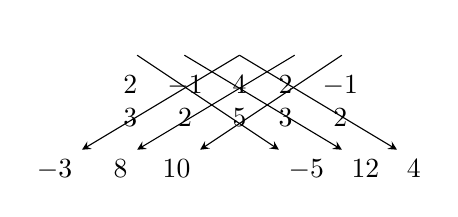
\begin{tikzpicture}[baseline=-3pt,>=stealth]
\node at (0,0) {$\begin{array}{ccccc} \ \veci\ &\ \vecj\ &\ \veck\ &\ \veci\ &\ \vecj\ \\  2&-1&4&2&-1\\3&2&5&3&2\end{array}$};
\draw[->,  thin] (-1.3,.4) -- (.5,-.8) node[below right] {$-5\veci$};
\draw[->,  thin] (-.7,.4) -- (1.3,-.8) node[below right ] {12\vecj};
\draw[->, thin] (0,.4) -- (2,-.8) node[below right] {4\veck};
\draw[->, thin] (0,.4) -- (-2,-.8) node[below left] {$-3\veck$};
\draw[->, thin] (.7,.4) -- (-1.3,-.8) node[below left ] {8\veci};
\draw[->, thin] (1.3,.4) -- (-.5,-.8) node[below left] {10\vecj};
\end{tikzpicture}\end{center}
\[\crossp uv = \big(-5\veci+12\vecj+4\veck\,\big) - \big(-3\veck+8\veci+10\vecj\,\big) = -13\veci+2\vecj+7\veck =\bracket{-13,2,7}.\]

This is equivalent to evaluating the determinant
\begin{align*}
 \begin{vmatrix}\veci&\vecj&\veck\\2&-1&4\\3&2&5\end{vmatrix}
 &=\begin{vmatrix}-1&4\\2&5\end{vmatrix}\veci
 -\begin{vmatrix}2&4\\3&5\end{vmatrix}\vecj
 +\begin{vmatrix}2&-1\\3&2\end{vmatrix}\veck \\
 &=(-5-8)\veci-(10-12)\vecj+(4-(-3))\veck
 =-13\veci+2\vecj+7\veck.
\end{align*}

We practice using this method.

\example{ex_crossp2}{Computing a cross product}{Let $\vecu=\bracket{1,3,6}$ and $\vec v = \bracket{-1,2,1}$. Compute both $\crossp uv$ and $\crossp vu$.}
{To compute $\crossp uv$, we form the matrix as prescribed above, complete with repeated first columns:
\[\begin{array}{ccccc} \ \veci\ &\ \vecj\ &\ \veck\ &\ \veci\ &\ \vecj\ \\  1&3&6&1&3\\-1&2&1&-1&2\end{array}\]
We let the reader compute the products of the diagonals; we give the result:
\[\crossp uv = \big(3\veci-6\vecj+2\veck\,\big) - \big(-3\veck + 12\veci+\vecj\,\big) = \bracket{-9,-7,5}.\]

To compute $\crossp vu$, we switch the second and third rows of the above matrix, then multiply along diagonals and subtract:

\[\begin{array}{ccccc} \ \veci\ &\ \vecj\ &\ \veck\ &\ \veci\ &\ \vecj\ \\-1&2&1&-1&2\\  1&3&6&1&3\end{array}\]
Note how with the rows being switched, the products that once appeared on the right now appear on the left, and vice-versa. Thus the result is:
\[\crossp vu = \big(12\veci+\vecj-3\veck\,\big) - \big(2\veck + 3\veci-6\vecj\,\big) = \bracket{9,7,-5},\]
which is the opposite of $\crossp uv$. We leave it to the reader to verify that each of these vectors is orthogonal to $\vec u$ and $\vec v$.}

\subsection{Properties of the Cross Product}

It is not coincidence that $\crossp vu = -(\crossp uv)$ in the preceding example; one can show using \autoref{def:cross_product} that this will always be the case. The following theorem states several useful properties of the cross product, each of which can be verified by referring to the definition.

\setboxwidth{15pt}
\theorem{thm:cross_prod_prop}{Properties of the Cross Product}
{Let $\vecu$, $\vecv$ and $\vecw$ be vectors in $\mathbb{R}^3$ and let $c$ be a scalar. The following identities hold:
\index{vectors!cross product}\index{cross product!properties}
\begin{enumerate}
	\item \parbox{167pt}{$\crossp uv = -(\crossp vu)$} Anticommutative Property
	\item	\begin{enumerate}
		\item \parbox{145pt}{$(\vec u+\vec v)\times \vecw = \crossp uw+\crossp vw$} Distributive Properties
		\item	$\vec u \times (\vec v+\vec w) = \crossp uv+\crossp uw$
	\end{enumerate}
	\item		$c(\crossp uv) = (c\vecu) \times \vec v = \vecu \times (c\vecv)$
	\item		\begin{enumerate}
		\item \parbox{145pt}{$(\crossp uv)\cdot \vecu = 0$} Orthogonality Properties
		\item	$(\crossp uv)\cdot \vecv = 0$
	\end{enumerate}
	\item		$\crossp uu = \vec 0$
	\item		$\crossp u0 = \vec 0$
	\item		\parbox{167pt}{$\vecu \cdot (\vecv\times\vecw) = (\crossp uv)\cdot \vecw$} Scalar Triple Product
\end{enumerate}}

We introduced the cross product as a way to find a vector orthogonal to two given vectors, but we did not give a proof that the construction given in \autoref{def:cross_product} satisfies this property. \autoref{thm:cross_prod_prop} asserts this property holds; we leave the verification to \exautoref{pr_cross_perp}.

Property 5 from the theorem is also left to the reader to prove in \exautoref{cross_self}, but it reveals something more interesting than ``the cross product of a vector with itself is $\vec 0$.'' Let $\vec u$ and $\vec v$ be parallel vectors; that is, let there be a scalar $c$ such that $\vecv = c\vecu$. Consider their cross product:
\begin{align*}
	\crossp uv
	&= \vecu \times (c\vec u) \\
	&= c(\crossp uu) & \text{(by Property 3 of \autoref{thm:cross_prod_prop})} \\
	&= \vec 0. & \text{(by Property 5 of \autoref{thm:cross_prod_prop})}
\end{align*}

We have just shown that the cross product of parallel vectors is $\vec 0$. This hints at something deeper. \autoref{thm:dot_product} related the angle between two vectors and their dot product; there is a similar relationship relating the cross product of two vectors and the angle between them, given by the following theorem.

\theorem{thm:cross_product}{The Cross Product and Angles}
{Let $\vec u$ and $\vec v$ be vectors in $\mathbb{R}^3$. Then
\[\norm{\crossp uv} = \vnorm u\, \vnorm v \sin\theta,\]
where $\theta$, $0\leq \theta \leq \pi$, is the angle between $\vecu$ and $\vecv$.
\index{vectors!cross product}\index{cross product!properties}}

\mnote{\textbf{Note:} \autoref{def:orthogonal} (through \autoref{thm:dot_product}) defines $\vec u$ and $\vec v$ to be orthogonal if $\vec u\cdot\vec v=0$. We could use \autoref{thm:cross_product} to define $\vec u$ and $\vec v$ are parallel if $\vec u\times \vec v = 0$. By such a definition, $\vec 0$ would be both orthogonal and parallel to every vector. Apparent paradoxes such as this are not uncommon in mathematics and can be very useful. (See also the marginal note%
\ifthenelse{\boolean{latexml}}{%
 \ at \autoref{def:parallel_vectors}%
}{%
 \ on \autopageref{note:parallel}%
}%
.)\label{note:crossp}}

Note that this theorem makes a statement about the \emph{magnitude} of the cross product. When the angle between $\vecu$ and $\vecv$ is 0 or $\pi$ (i.e., the vectors are parallel), the magnitude of the cross product is 0. The only vector with a magnitude of 0 is $\vec 0$ (see Property \ref{thm:zero_norm} of \autoref{thm:vector_properties}), hence the cross product of  parallel vectors is $\vec 0$.\bigskip

We demonstrate the truth of this theorem in the following example.

\example{ex_crossp3}{The cross product and angles}{Let $\vec u =\bracket{1,3,6}$ and $\vec v = \bracket{-1,2,1}$ as in \autoref{ex_crossp2}. Verify \autoref{thm:cross_product} by finding $\theta$, the angle between $\vecu$ and $\vecv$, and the magnitude of $\crossp uv$.}
{We use \autoref{thm:dot_product} to find the angle between $\vecu$ and $\vecv$. 
\begin{align*}
\theta &= \cos^{-1}\left(\frac{\vec u\cdot\vec v}{\vnorm u\, \vnorm v}\right) \\
			&= \cos^{-1}\left(\frac{11}{\sqrt{46}\sqrt{6}}\right)\\
			&\approx 0.8471 = 48.54^\circ.
\end{align*}

Our work in \autoref{ex_crossp2} showed that $\crossp uv = \bracket{-9,-7,5}$, hence $\norm{\crossp uv} = \sqrt{155}.$ Is $\norm{\crossp uv} = \vnorm u\, \vnorm v\sin\theta$? Using numerical approximations, we find:
\begin{align*}
\norm{\crossp uv}
 &=\sqrt{155}  & \vnorm u\,\vnorm v \sin\theta & = \sqrt{46}\sqrt{6}\sin 0.8471\\
 &\approx 12.45. & &\approx 12.45.
\end{align*}
Numerically, they seem equal. Using a right triangle, one can show that 
\[\sin\left(\cos^{-1}\left(\frac{11}{\sqrt{46}\sqrt{6}}\right)\right) = \frac{\sqrt{155}}{\sqrt{46}\sqrt{6}},\]
which allows us to verify the theorem exactly.}

\subsection{Right Hand Rule}

The anticommutative property of the cross product demonstrates that $\crossp uv$ and $\crossp vu$ differ only by a sign --- these vectors have the same magnitude but point in the opposite direction. When seeking a vector perpendicular to $\vec u$ and $\vec v$, we essentially have two directions to choose from, one in the direction of $\crossp uv$ and one in the direction of $\crossp vu$. Does it matter which we choose? How can we tell which one we will get without graphing, etc.?

\mtable{Illustrating the Right Hand Rule of the cross product.}{fig:crossp_rhr}{
\myincludeasythree{width=\marginparwidth,
3Droll=0,
3Dortho=0.0044,
3Dc2c=.78 .32 .53,
3Dcoo=0 0 34,
3Droo=150}{width=\marginparwidth}{figures/figcrossp_rhr_3D}}

Another property of the cross product, as defined, is that it follows the \textbf{right hand rule.} Given $\vec u$ and $\vec v$ in $\mathbb{R}^3$ with the same initial point, point the index finger of your right hand in the direction of $\vecu$ and let your middle finger point in the direction of $\vecv$ (much as we did when establishing the right hand rule for the 3-dimensional coordinate system). Your thumb will naturally extend in the direction of $\crossp uv$. One can ``practice'' this using \autoref{fig:crossp_rhr}. If you switch, and point the index finder in the direction of $\vecv$ and the middle finger in the direction of $\vecu$, your thumb will now point in the opposite direction, allowing you to ``visualize'' the anticommutative property of the cross product.  In fact, we can use this property to define the cross product, which we summarize in the next key idea.

\keyidea{ki:cross_prod_alt}{Alternate Definition of the Cross Product}{For vectors $\vecu$ and $\vecv$, the cross product $\vecu\times\vecv$ is the unique vector such that
\begin{enumerate}
\item $\norm{\vecu\times\vecv}=\norm{\vecu}\norm{\vecv}\sin\theta$ where $\theta$ is the angle between $\vecu$ and $\vecv$,
\item $\vecu\times\vecv$ is orthogonal to both $\vecu$ and $\vecv$, 
and
\item $\vecu$, $\vecv$, and $\vecu\times\vecv$ form a right-handed triple.
\end{enumerate}}

\subsection{Applications of the Cross Product}

There are a number of ways in which the cross product is useful in mathematics, physics and other areas of science beyond ``just'' finding a vector perpendicular to two others. We highlight a few here.\index{cross product!applications}

\subsubsection{Area of a Parallelogram}

\mtable{Using the cross product to find the area of a parallelogram.}{fig:crossp_parallelogram}{%
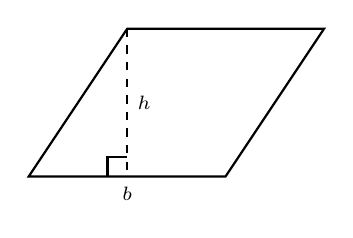
\begin{tikzpicture}[thick,scale=1.25]
 \draw(0,0)--node[below,pos=.5]{\scriptsize $b$}(2,0)--(3,1.5)--(1,1.5)--cycle;
 \draw [dashed] (1,1.5) -- (1,0) node [pos=.5,right] {\scriptsize$h$};
 \draw (.8,0) -- (.8,.2) -- (1,.2);
\end{tikzpicture}
\\(a) \\[15pt]
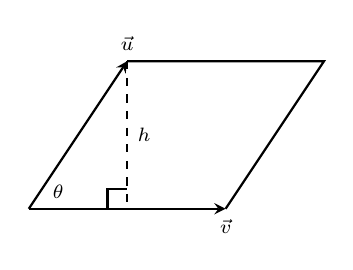
\begin{tikzpicture}[thick,scale=1.25,>=stealth]
	\draw [->](0,0) -- node [below,pos=1]  {\scriptsize $\vec v$} (2,0);
	\draw (2,0) -- (3,1.5) -- (1,1.5);
	\draw (.3,.175) node {\scriptsize $\theta$};
	\draw [->](0,0) -- (1,1.5) node [above] {\scriptsize $\vec u$};
	\draw [dashed] (1,1.5) -- (1,0) node [pos=.5,right] {\scriptsize$h$};
	\draw (.8,0) -- (.8,.2) -- (1,.2);
\end{tikzpicture}
\\(b)}

It is a standard geometry fact that the area of a parallelogram is $A = bh$, where $b$ is the length of the base and $h$ is the height of the parallelogram, as illustrated in \autoref{fig:crossp_parallelogram}(a). As shown when defining the Parallelogram Law of vector addition, two vectors $\vecu$ and $\vecv$ define a parallelogram when drawn from the same initial point, as illustrated in \autoref{fig:crossp_parallelogram}(b). Trigonometry tells us that $h = \vnorm u \sin \theta$, hence the area of the parallelogram is 
\begin{equation}A = \vnorm u\,\vnorm v\sin\theta = \norm{\crossp uv},\label{eq:crossp1}\end{equation}
where the second equality comes from \autoref{thm:cross_product}.
We illustrate using \autoeqref{eq:crossp1} in the following example.
\index{cross product!applications!area of parallelogram}

\example{ex_crossp4}{Finding the area of a parallelogram}{\mbox{}\\[-2\baselineskip]\begin{enumerate}
	\item Find the area of the parallelogram defined by the vectors $\vecu = \bracket{2,1}$ and $\vecv = \bracket{1,3}$.
	\item	Verify that the points $A = (1,1,1)$, $B = (2,3,2)$, $C = (4,5,3)$ and $D = (3,3,2)$ are the vertices of a parallelogram. Find the area of the parallelogram.
\end{enumerate}}
{\mbox{}\\[-1.5\baselineskip]\begin{enumerate}
	\item \autoref{fig:crossp4}(a) sketches the parallelogram defined by the vectors $\vec u$ and $\vec v$. We have a slight problem in that our vectors exist in $\mathbb{R}^2$, not $\mathbb{R}^3$, and the cross product is only defined on vectors in $\mathbb{R}^3$. We skirt this issue by viewing $\vec u$ and $\vecv$ as vectors in the $x-y$ plane of $\mathbb{R}^3$, and rewrite them as $\vec u = \bracket{2,1,0}$ and $\vecv =\bracket{1,3,0}$. We can now compute the cross product.
%
% todo Tim this parallelogram is very narrow.  do we want something better?
\mtable[-6\baselineskip]{Sketching the parallelograms in \autoref{ex_crossp4}.}{fig:crossp4}{%
\begin{tikzpicture}
\begin{axis}[width=1.16\marginparwidth,tick label style={font=\scriptsize},
axis y line=middle,axis x line=middle,name=myplot,axis on top,xtick={1,2,3,4},
ytick={1,2,3,4,5},ymin=-.5,ymax=5.5,xmin=-.5,xmax=4.5]
\draw[thick,->,>=stealth] (axis cs:0,0) --(axis cs:2,1)
 node [right] {\scriptsize $\vec u$};
\draw[thick,->,>=stealth] (axis cs:0,0) --(axis cs:1,3)
 node [above] {\scriptsize $\vec v$};
\draw[thick] (axis cs:2,1) --(axis cs:3,4) -- (axis cs: 1,3);
\end{axis}
\node [right] at (myplot.right of origin) {\scriptsize $x$};
\node [above] at (myplot.above origin) {\scriptsize $y$};
\end{tikzpicture}
	\\(a)\\%[15pt]
	\myincludeasythree{width=\marginparwidth,
3Droll=0.767,
3Dortho=0.004,
3Dc2c=-0.34424060583114624 -0.8107251524925232 0.47352203726768494,
3Dcoo=61 60 63,
3Droo=250}{width=\marginparwidth}{figures/figcrossp4a_3D}\\
	(b)}
%
It is easy to show that $\crossp uv = \bracket{0,0,5}$; therefore the area of the parallelogram is $A = \norm{\crossp uv} = 5$.
	\item		To show that the quadrilateral $ABCD$ is a parallelogram (shown in \autoref{fig:crossp4}(b)), we need to show that the opposite sides are parallel. We can quickly show that $\vv{AB} =\vv{DC} = \bracket{1,2,1}$ and $\vv{BC} = \vv{AD} = \bracket{2,2,1}$. We find the area by computing the magnitude of the cross product of $\vv{AB}$ and $\vv{BC}$:
	\[
	\vv{AB} \times \vv{BC} = \bracket{0,1,-2}\quad \Rightarrow \quad
	\norm{\vv{AB}\times\vv{BC}} = \sqrt{5}.\eoehere
	\]%  \approx 2.236
\end{enumerate}}

This application is more commonly used to find the area of a triangle (because triangles are used more often than parallelograms). We illustrate this in the following example.

\example{ex_crossp5}{Area of a triangle}{Find the area of the triangle with vertices $A=(1,2)$, $B=(2,3)$ and $C=(3,1)$, as pictured in \autoref{fig:crossp5}.}
{We found the area of this triangle in \autoref{ex_abc4} to be $1.5$ using integration. There we discussed the fact that finding the area of a triangle can be inconvenient using the ``$\frac12bh$'' formula as one has to compute the height, which generally involves finding angles, etc. Using a cross product is much more direct.

\mtable{Finding the area of a triangle in \autoref{ex_crossp5}.}{fig:crossp5}{\begin{tikzpicture}
\begin{axis}[width=1.16\marginparwidth,tick label style={font=\scriptsize},
axis y line=middle,axis x line=middle,name=myplot,axis on top,
xtick={1,2,3},ymin=-.1,ymax=3.5,xmin=-.1,xmax=3.9]
\addplot [{\colorone},thick,fill={\coloronefill}] coordinates {(1,2) (2,3) (3,1) (1,2)};
\draw (axis cs:1,2) node [left]{\scriptsize $A$} (axis cs:2,3) node [above] {\scriptsize $B$} (axis cs:3,1) node [below] {\scriptsize $C$};
\end{axis}
\node [right] at (myplot.right of origin) {\scriptsize $x$};
\node [above] at (myplot.above origin) {\scriptsize $y$};
\end{tikzpicture}}

We can choose any two sides of the triangle to use to form vectors; we choose $\vv{AB} = \bracket{1,1}$ and $\vv{AC}=\bracket{2,-1}$. As in the previous example, we will rewrite these vectors with a third component of 0 so that we can apply the cross product. The area of the triangle is
\[
\frac12\norm{\vv{AB}\times\vv{AC}}
= \frac12\norm{\bracket{1,1,0}\times \bracket{2,-1,0}}
= \frac12\norm{\bracket{0,0,-3}} = \frac32.
\]
We arrive at the same answer as before with less work.}

\subsubsection{Volume of a Parallelepiped}

The three dimensional analogue to the parallelogram is the \textbf{parallelepiped}.
Each face is parallel to the opposite face, as illustrated in \autoref{fig:crossp_parallelepiped}. By crossing $\vec v$ and $\vec w$, one gets a vector whose magnitude is the area of the base. Dotting this vector with $\vecu$ computes the volume of parallelepiped! (Up to a sign; take the absolute value.)

\mnote[-5\baselineskip]{\textbf{Note:} The word ``parallelepiped'' is pronounced ``parallel-eh-pipe-ed.''}%
%
\mtable{A parallelepiped is the three dimensional analogue to the parallelogram.}{fig:crossp_parallelepiped}{%
\myincludeasythree{width=.5\marginparwidth,
3Droll=0,
3Dortho=0.0045,
3Dc2c=.84 .46 .26,
3Dcoo=0 110 86,
3Droo=150}{width=.5\marginparwidth}{figures/figcrosspparallelpiped_3D}}%
%
\index{cross product!applications!volume of parallelepiped}%

Thus the volume of a parallelepiped defined by vectors $\vecu$, $\vecv$ and $\vec w$ is
\begin{equation}
V = \abs{\vecu\cdot (\crossp vw)}.\label{eq:crossp2}
\end{equation}
Note how this is the Scalar Triple Product, first seen in \autoref{thm:cross_prod_prop}. Applying the identities given in the theorem shows that we can apply the Scalar Triple Product in any ``order'' we choose to find the volume. That is,
\[V = \abs{\vecu\cdot(\crossp vw)} = \abs{\vec u\cdot (\crossp wv)} = \abs{(\crossp uv)\cdot \vecw},\quad \text{etc.}\]
As with the cross product, we can also write $\vecu\cdot(\crossp vw)$ in terms of a determinant:
\[
 \vecu\cdot(\crossp vw)=
 \begin{vmatrix}u_1&u_2&u_3\\v_1&v_2&v_3\\w_1&w_2&w_3\end{vmatrix}.
\]
Because the volume is the absolute value of the determinant, changing the order of the rows can only change the sign of this determinant, which doesn't change the final answer.

\mtable{A parallelepiped in \autoref{ex_crossp6}.}{fig:crossp6}{
\myincludeasythree{width=\marginparwidth,
3Droll=0,
3Dortho=0.0045,
3Dc2c=4 4 2,
3Dcoo=0 50 50,
3Droo=150}{width=\marginparwidth}{figures/figcrossp6_3D}}

\example{ex_crossp6}{Finding the volume of parallelepiped}{Find the volume of the parallelepiped defined by the vectors $\vecu = \bracket{1,1,0}$, $\vecv = \bracket{-1,1,0}$ and $\vecw = \bracket{0,1,1}$.}
{We apply \autoeqref{eq:crossp2}. We first find $\crossp vw =\bracket{1,1,-1}$. Then
\[\abs{\vec u\cdot(\crossp vw)} = \abs{\bracket{1,1,0}\cdot \bracket{1,1,-1}} = 2.\]
So the volume of the parallelepiped is 2 cubic units.  In terms of determinants, we have
\[
 \begin{vmatrix}1&1&0\\-1&1&0\\0&1&1\end{vmatrix}
 =\begin{vmatrix}1&0\\1&1\end{vmatrix}1
 -\begin{vmatrix}-1&0\\0&1\end{vmatrix}1
 +\begin{vmatrix}-1&1\\0&1\end{vmatrix}0
 (1-0)1-(-1-0)1
 =1+1
 =2,
\]
and the absolute value of this determinant is again 2.}

%While this application of the Scalar Triple Product is interesting, it is not used all that often: parallelepipeds are not a common shape in physics and engineering.
%% On the other hand, a tetrahedron is more common of a shape, and its volume is $\frac16$ that of a parallelepiped formed with the same vectors.
%The last application of the cross product is very applicable in engineering.

\subsubsection{Torque}

\textbf{Torque} is a measure of the turning force applied to an object. A classic scenario involving torque is the application of a wrench to a bolt. When a force is applied to the wrench, the bolt turns. When we represent the force and wrench with vectors $\vec F$ and $\vec \ell$, we see that the bolt moves (because of the threads) in a  direction orthogonal to $\vec F$ and $\vec \ell$. Torque is usually represented by the Greek letter $\tau$, or tau, and has units of N$\cdot$m, a newton-meter, or ft$\cdot$lb, a foot-pound.\index{cross product!applications!torque}

While a full understanding of torque is beyond the purposes of this book, when a force $\vec F$ is applied to a lever arm $\vec \ell$, the resulting torque is \begin{equation}\vec \tau = \crossp \ell F.\label{eq:crossp3}\end{equation}

\example{ex_crossp7}{Computing torque}{A lever of length 2ft makes an angle with the horizontal of $45^\circ$. Find the resulting torque when a force of 10lb is applied to the end of the level where:

\mtable{Showing a force being applied to a lever in \autoref{ex_crossp7}.}{fig:crossp7}{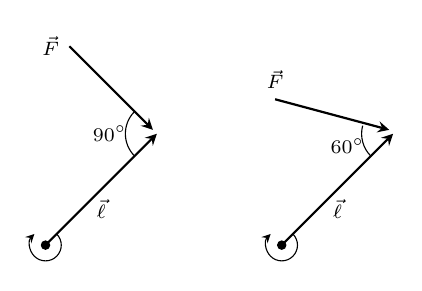
\begin{tikzpicture}[>=stealth]
 \draw [thick,->,rotate=45] (-2,0) -- (0,0)
  node [below,pos=.5] {\scriptsize $\vec\ell$};
 \filldraw[black,rotate=45] (-2,0) circle (1.5pt);
 \draw [rotate=45,->] (-1.8,0) arc (0:-270:.2);
 \draw[rotate=45] (-.4,0) arc (180:90:.4);
 \draw [rotate=0] (-.6,0) node {\scriptsize $90^\circ$};
 \begin{scope}[shift={(-.05,.05)}]
  \draw [thick,->,rotate=-45] (-1.5,0)node [left] {\scriptsize $\vec F$} -- (0,0);
 \end{scope}
 \begin{scope}[shift={(3,0)}]
  \draw [thick,->,rotate=45] (-2,0) -- (0,0)
   node [below,pos=.5] {\scriptsize $\vec\ell$};
  \filldraw[black,rotate=45] (-2,0) circle (1.5pt);
  \draw [rotate=45,->] (-1.8,0) arc (0:-270:.2);
  \draw[rotate=45] (-.4,0) arc (180:120:.4);
  \draw [rotate=15] (-.6,0) node {\scriptsize $60^\circ$};
  \begin{scope}[shift={(-.05,.05)}]
   \draw [thick,->,rotate=-15] (-1.5,0)node [above] {\scriptsize $\vec F$} -- (0,0);
  \end{scope}
 \end{scope}
\end{tikzpicture}}

\begin{enumerate}
	\item the force is perpendicular to the lever, and
	\item	the force makes an angle of $60^\circ$ with the lever, as shown in \autoref{fig:crossp7}.
\end{enumerate}}
{\begin{enumerate}
	\item We start by determining vectors for the force and lever arm. Since the lever arm makes a $45^\circ$ angle with the horizontal and is 2ft long, we can state that $\vec \ell = 2\bracket{\cos 45^\circ,\sin 45^\circ}= \bracket{\sqrt2,\sqrt2}.$
	
	Since the force vector is perpendicular to the lever arm (as seen in the left hand side of \autoref{fig:crossp7}), we can conclude it is making an angle of $-45^\circ$ with the horizontal. As it has a magnitude of 10lb, we can state $\vec F = 10\bracket{\cos (-45^\circ), \sin(-45^\circ)}= \bracket{5\sqrt2,-5\sqrt2}.$
	
	Using \autoeqref{eq:crossp3} to find the torque requires a cross product. We again let the third component of each vector be 0  and compute the cross product:
	\begin{align*}
	\vec\tau &= \crossp \ell F \\
				&= \bracket{\sqrt2,\sqrt2,0}\times \bracket{5\sqrt2,-5\sqrt2,0}\\
				&= \bracket{0,0,-20}
	\end{align*}
	This clearly has a magnitude of 20 ft-lb.
		
	We can view the force and lever arm vectors as lying ``on the page''; our computation of $\vec\tau$ shows that the torque goes ``into the page.'' This follows the Right Hand Rule of the cross product, and it also matches well with the example of the wrench turning the bolt. Turning a bolt clockwise moves it in.
	
	\item		Our lever arm can still be represented by $\vec \ell = \bracket{\sqrt2,\sqrt2}$. As our force vector makes a $60^\circ$ angle with $\vec \ell$, we can see (referencing the right hand side of the figure) that $\vec F$ makes a $-15^\circ$ angle with the horizontal. Thus 
	\begin{align*}
	\vec F = 10\bracket{\cos-15^\circ,\sin-15^\circ}&= \bracket{\frac{5(1+\sqrt3)}{\sqrt2},\frac{5(1-\sqrt3)}{\sqrt2}}
	%\\&\approx \bracket{9.659,-2.588}
	.\end{align*}
	
	We again make the third component 0 and take the cross product to find the torque:
	\begin{align*}
	\vec\tau &= \crossp \ell F\\
	&= \bracket{\sqrt2,\sqrt2,0}\times  \bracket{\frac{5(1+\sqrt3)}{\sqrt2},\frac{5(1-\sqrt3)}{\sqrt2},0}\\
	&= \bracket{0,0,-10\sqrt3}
	%\\&\approx \bracket{0,0,-17.321}
	.
	\end{align*}
	As one might expect, when the force and lever arm vectors \textit{are} orthogonal, the magnitude of force is greater than when the vectors \textit{are not} orthogonal.\eoehere
\end{enumerate}}

While the cross product has a variety of applications (as noted in this chapter), its fundamental use is finding a vector perpendicular to two others. Knowing a vector is orthogonal to two others is of incredible importance, as it allows us to find the equations of lines and planes in a variety of contexts. The importance of the cross product, in some sense, relies on the importance of lines and planes, which see widespread use throughout engineering, physics and mathematics. We study lines and planes in the next two sections. 

\printexercises{exercises/10_04_exercises}


\section{Lines}\label{sec:lines}

\index{lines}
To find the equation of a line in the $x$-$y$ plane, we need two pieces of information: a point and the slope. The slope conveys \textit{direction} information. As vertical lines have an undefined slope, the following statement is more accurate:

\begin{quotation}
\noindent To define a line, one needs a point on the line and the direction of the line.
\end{quotation}

This holds true for lines in space.\bigskip

Let $P$ be a point in space, let $\vec p$ be the vector with initial point at the origin and terminal point at $P$ (i.e., $\vec p$ ``points'' to $P$), and let $\vec d$ be a vector. Consider the points on the line through $P$ in the direction of $\vec d$. 

Clearly one point on the line is $P$; we can say that the \emph{vector} $\vec p$ lies at this point on the line. To find another point on the line, we can start at $\vec p$ and move in a  direction parallel to $\vec d$. For instance, starting at $\vec p$ and traveling one length of $\vec d$ places one at another point on the line. Consider \autoref{fig:lines_intro} where certain points along the line are indicated.

\mtable{Defining a line in space.}{fig:lines_intro}{%
\myincludeasythree{width=\marginparwidth,
3Droll=0,
3Dortho=0.0045,
3Dc2c=.84 .46 .26,
3Dcoo=0 70 0,
3Droo=150}{width=\marginparwidth}{figures/figlines_intro_3D}}

The figure illustrates how every point on the line can be obtained by starting with $\vec p$ and moving a certain distance in the direction of $\vec d$. That is, we can define the line as a function of $t$:
\begin{equation}\vec\ell(t) = \vec p + t\ \vec d.\label{eq:lines1}\end{equation}

In many ways, this is \textit{not} a new concept. Compare \autoeqref{eq:lines1} to the familiar ``$y=mx+b$'' equation of a line:

\begin{figure}[!hb]
\centering
\begin{tikzpicture}[>=stealth]
	\draw (0,0) node (L) {\large $y\ =\ b\ +\ m\,x$};
	\draw (5,0) node (R) {\large $\vec \ell(t)\ =\ \vec p\ +\ t\,\vec d$};
\node (A) at (1,1.5) {\begin{tabular}{c}Starting\\Point\end{tabular}};
%\node (A) at (1,1.5) [align=center] {Starting\\ Point};
\node (B) at (4,1.5) {Direction};
\node (C) at (2.5,-1.5) {\begin{tabular}{c}How Far To\\Go In That\\Direction\end{tabular}};
%\node (C) at (2.5,-1.5) [align=center] {How Far To\\  Go In That \\Direction};
\draw [->,thick] (A) -- ($(R)+(-1pt,8pt)$);
\draw [->,thick] (A) -- ($(L)+(-0pt,10pt)$);
\draw [->,thick] (B) -- (.9,.2);
\draw [->,thick] (B) -- ($(R)+(30pt,7pt)$);
\draw [->,thick] (C) -- (1.3,-.15);
\draw [->,thick] (C) -- ($(R)+(25pt,-7pt)$);
\end{tikzpicture}
\captionsetup{type=figure}%
\caption{Understanding the vector equation of a line.}
\label{fig:lines_eq}
\end{figure}

The equations exhibit the same structure: they give a starting point, define a direction, and state how far in that direction to travel.

\autoeqref{eq:lines1} is an example of a \textbf{vector-valued function}; the input of the function is a real number and the output is a vector. We will cover vector-valued functions extensively in the next chapter.

There are other ways to represent a line. Let $\vec p =\bracket{x_0,y_0,z_0}$ and let $\vec d =\bracket{a,b,c}$. Then the equation of the line through $\vec p$ in the direction of $\vec d$ is:
\begin{align*}
\vec\ell(t) &= \vec p + t\vec d \\
						&=\bracket{x_0,y_0,z_0}+ t\bracket{a,b,c}\\
						&=\bracket{x_0 + at, y_0+bt, z_0+ct}.
\end{align*}

The last line states the the $x$ values of the line are given by $x=x_0+at$, the $y$ values are given by $y = y_0+bt$, and the $z$ values are given by $z = z_0 + ct$. These three equations, taken together, are the \textbf{parametric equations of the line} through $\vec p$ in the direction of $\vec d$.

Finally, each of the equations for $x$, $y$ and $z$ above contain the variable $t$. We can solve for $t$ in each equation:
\begin{align*}
x = x_0+at \quad&\Rightarrow\quad t = \frac{x-x_0}{a},\\
y = y_0+bt \quad&\Rightarrow\quad t = \frac{y-y_0}{b},\\
z = z_0+ct \quad&\Rightarrow\quad t = \frac{z-z_0}{c},\\
\end{align*}
assuming $a,b,c\neq 0$.
Since $t$ is equal to each expression on the right, we can set these equal to each other, forming the \textbf{symmetric equations of the line} through $\vec p$ in the direction of $\vec d$:
\[\frac{x-x_0}{a} = \frac{y-y_0}{b}=\frac{z-z_0}{c}.\]
Each representation has its own advantages, depending on the context. We summarize these three forms in the following definition, then give examples of their use.

\definition{def:lines}{Equations of Lines in Space}
{Consider the line in space that passes through $\vec p =\bracket{x_0,y_0,z_0}$ in the direction of $\vec d =\bracket{a,b,c}.$\index{lines!equations for}
\begin{enumerate}
	\item The \textbf{vector equation} of the line is
	\[\vec \ell(t) = \vec p+t\vec d.\]
	\item	The \textbf{parametric equations} of the line are
	\[x = x_0+at, \quad y=y_0+bt, \quad z = z_0+ct .\]
	\item	The \textbf{symmetric equations} of the line are
	\[\frac{x-x_0}{a} = \frac{y-y_0}{b}=\frac{z-z_0}{c}.\]
\end{enumerate}}

\youtubeVideo{q4wDcrCkkfQ}{Example of Symmetric Equations of a Line}

\example{ex_lines1}{Finding the equation of a line}{Give all three equations, as given in \autoref{def:lines}, of the line through $P = (2,3,1)$ in the direction of $\vec d =\bracket{-1,1,2}$. Does the point $Q=(-1,6,6)$ lie on this line?}
{We identify the point $P=(2,3,1)$ with the vector $\vec p =\bracket{2,3,1}$. Following the definition, we have
\begin{itemize}
	\item the vector equation of the line is $\vec\ell(t) =\bracket{2,3,1}+ t\bracket{-1,1,2}$;
	\item	the parametric equations of the line are
	\[x = 2-t,\quad y = 3+t,\quad z = 1+2t; \text{ and}\]
	\item	the symmetric equations of the line are
	\[\frac{x-2}{-1}=\frac{y-3}{1} = \frac{z-1}{2}.\]
\end{itemize}

The first two equations of the line are useful when a $t$ value is given: one can immediately find the corresponding point on the line. These forms are good when calculating with a computer; most software programs easily handle equations in these formats.
\mtable{Graphing a line in \autoref{ex_lines1}.}{fig:lines1}{%
\myincludeasythree{width=\marginparwidth,
3Droll=0,
3Dortho=0.0045,
3Dc2c=.78 .53 .32,
3Dcoo=0 70 50,
3Droo=150}{width=\marginparwidth}{figures/figlines1_3D}}

%(For instance, to make \autoref{fig:lines1}, a certain graphics program was given the input \texttt{(2-x,3+x,1+2*x)}. This particular program requires the variable always be ``$x$'' instead of ``$t$'').

Does the point $Q = (-1,6,6)$ lie on the line? The graph in \autoref{fig:lines1} makes it clear that it does not. We can answer this question without the graph using any of the three equation forms. Of the three, the symmetric equations are probably best suited for this task. Simply plug in the values of $x$, $y$ and $z$ and see if equality is maintained:
\[
\frac{-1-2}{-1} \stackrel{?}{=} \frac{6-3}{1} \stackrel{?}{=} \frac{6-1}{2}
\quad \Rightarrow \quad 3=3\neq2.5.
\]
We see that $Q$ does not lie on the line as it did not satisfy the symmetric equations.}

\example{ex_lines6}{Finding the equation of a line through two points}{Find the parametric equations of the line through the points $P=(2,-1,2)$ and $Q = (1,3,-1)$.}
{Recall the statement made at the beginning of this section: to find the equation of a line, we need a point and a direction. We have \emph{two} points; either one will suffice. The direction of the line can be found by the vector with initial point $P$ and terminal point $Q$: $\vv{PQ} =\bracket{-1,4,-3}$.

The parametric equations of the line $\ell$ through $P$ in the direction of $\vv{PQ}$ are:
\[\ell: \quad x= 2-t\quad y=-1+4t \quad z=2-3t.\]

\mtable{A graph of the line in \autoref{ex_lines6}.}{fig:lines6}{%
\myincludeasythree{width=\marginparwidth,
3Droll=0,
3Dortho=0.0045,
3Dc2c=.4 .87 .32,
3Dcoo=58 8.7 4.6,
3Droo=150}{width=\marginparwidth}{figures/figlines6_3D}}

A graph of the points and line are given in \autoref{fig:lines6}. Note how in the given parameterization of the line, $t=0$ corresponds to the point $P$, and $t=1$ corresponds to the point $Q$. This relates to the understanding of the vector equation of a line described in \autoref{fig:lines_eq}. The parametric equations ``start'' at the point $P$, and $t$ determines how far in the direction of $\vv{PQ}$ to travel. When $t=0$, we travel 0 lengths of $\vv{PQ}$; when $t=1$, we travel one length of $\vv{PQ}$, resulting in the point $Q$.}

\subsection{Parallel, Intersecting and Skew Lines}

In the plane, two \emph{distinct} lines can either be parallel or they will intersect at exactly one point. In space, given equations of two lines, it can sometimes be difficult to tell whether the lines are distinct or not (i.e., the same line can be represented in different ways). Given lines $\vec\ell_1(t) = \vec p_1 + t\vec d_1$ and $\vec \ell_2(t) = \vec p_2+t\vec d_2$, we have four possibilities: $\vec \ell_1$ and $\vec \ell_2$ are
\begin{center}
\begin{tabular}{p{100pt}p{150pt}}
the same line & they share all points; \\
intersecting lines & share only 1 point;\\
parallel lines & $\vec d_1\parallel \vec d_2$, no points in common; or \\
skew lines & $\vec d_1\nparallel \vec d_2$, no points in common. 
\end{tabular}
\end{center}
\index{lines!skew}\index{lines!parallel}\index{lines!intersecting}

The next two examples investigate these possibilities.

\example{ex_lines2}{Comparing lines}{Consider lines $\ell_1$ and $\ell_2$, given in parametric equation form:
\[
\ell_1: \begin{array}{ccc} x&=&1+3t \\ y&=&2-t\\z&=&t\end{array}
\qquad\qquad
\ell_2: \begin{array}{ccc} x&=&-2+4s\\y&=&3+s\\z&=&5+2s.\end{array}
\]
Determine whether $\ell_1$ and $\ell_2$ are the same line, intersect, are parallel, or skew.}
{We start by looking at the directions of each line. Line $\ell_1$ has the direction given by $\vec d_1=\bracket{3,-1,1}$ and line $\ell_2$ has the direction given by $\vec d_2 =\bracket{4,1,2}$. It should be clear that $\vec d_1$ and $\vec d_2$ are not parallel, hence $\ell_1$ and $\ell_2$ are not the same line, nor are they parallel. \autoref{fig:lines2} verifies this fact (where the points and directions indicated by the equations of each line are identified).

\mtable{Sketching the lines from \autoref{ex_lines2}.}{fig:lines2}{%
\myincludeasythree{width=\marginparwidth,
3Droll=0,
3Dortho=0.0045,
3Dc2c=.42 .80 .43,
3Dcoo=0 30 50,
3Droo=150}{width=\marginparwidth}{figures/figlines2_3D}}

We next check to see if they intersect (if they do not, they are skew lines). To find if they intersect, we look for $t$ and $s$ values such that the respective $x$, $y$ and $z$ values are the same. That is, we want $s$ and $t$ such that:
\[
\begin{array}{ccc}
1+3t &=&-2+4s\\
2-t&=&3+s\\
t&=&5+2s.\end{array}
\]
This is a relatively simple system of linear equations. Since the last equation is already solved for $t$, substitute that value of $t$ into the equation above it:
\[2-(5+2s) = 3+s \quad \Rightarrow \quad s=-2,\ t=1.\]
A key to remember is that we have \emph{three} equations; we need to check if $s=-2,\ t=1$ satisfies the first equation as well:
\[1+3(1) \neq -2+4(-2).\]
It does not. Therefore, we conclude that the lines $\ell_1$ and $\ell_2$ are skew.}

\example{ex_lines3}{Comparing lines}{Consider lines $\ell_1$ and $\ell_2$, given in parametric equation form:
\[
\ell_1: \begin{array}{ccc} x&=&-0.7+1.6t \\ y&=&4.2+2.72t\\z&=&2.3-3.36t\end{array}\qquad\qquad \ell_2:\begin{array}{ccc} x&=&2.8-2.9s\\y&=&10.15-4.93s\\z&=&-5.05+6.09s.\end{array}
\]
Determine whether $\ell_1$ and $\ell_2$ are the same line, intersect, are parallel, or skew.}
{It is obviously very difficult to simply look at these equations and discern anything. This is done intentionally. In the ``real world,'' most equations that are used do not have nice, integer coefficients.% Rather, there are lots of digits after the decimal and the equations can look ``messy.''

We again start by deciding whether or not each line has the same direction. The direction of $\ell_1$ is given by $\vec d_1 =\bracket{1.6,2.72,-3.36}$ and the direction of $\ell_2$ is given by $\vec d_2 =\bracket{-2.9,-4.93,6.09}$. When it is not clear through observation whether two vectors are parallel or not, the standard way of determining this is by comparing their respective unit vectors. Using a calculator, we find:
\begin{align*}
\vec u_1 &= \frac{\vec d_1}{\norm{\vec d_1}} =\bracket{0.3471,0.5901,-0.7289}\\
 \vec u_2 &= \frac{\vec d_2}{\norm{\vec d_2}} =\bracket{-0.3471,-0.5901,0.7289}.
\end{align*}

The two vectors seem to be parallel (at least, their components are equal to 4 decimal places). In most situations, it would suffice to conclude that the lines are at least parallel, if not the same. One way to be sure is to rewrite $\vec d_1$ and $\vec d_2$ in terms of fractions, not decimals. We have 
\[\vec d_1 =\bracket{\frac{16}{10},\frac{272}{100},-\frac{336}{100}}\qquad \vec d_2 =\bracket{-\frac{29}{10},-\frac{493}{100},\frac{609}{100}}.\]
% todo Tim why not just rescale d2 to match d1?
One can then find the magnitudes of each vector in terms of fractions, then compute the unit vectors likewise. After a lot of manual arithmetic (or after briefly using a computer algebra system), one finds that 
\[\vec u_1 =\bracket{\sqrt{\frac{10}{83}},\frac{17}{\sqrt{830}},-\frac{21}{\sqrt{830}}}\qquad \vec u_2 =\bracket{-\sqrt{\frac{10}{83}},-\frac{17}{\sqrt{830}},\frac{21}{\sqrt{830}}}.\]
We can now say without equivocation that these lines are parallel.

Are they the same line? The parametric equations for a line describe one point that lies on the line, so we know that the point $P_1 = (-0.7,4.2,2.3)$ lies on $\ell_1$. To determine if this point also lies on $\ell_2$, plug in the $x$, $y$ and $z$ values of $P_1$ into the symmetric equations for $\ell_2$:
\begin{multline*}
\frac{(-0.7)-2.8}{-2.9} \stackrel{?}{=} \frac{(4.2)-10.15}{-4.93} \stackrel{?}{=} \frac{(2.3)-(-5.05)}{6.09} \\
\Rightarrow \quad 1.2069=1.2069=1.2069.
\end{multline*}
\mtable[-5\baselineskip]{Graphing the lines in \autoref{ex_lines3}.}{fig:lines3}{%
\myincludeasythree{width=\marginparwidth,
3Droll=0,
3Dortho=0.0045,
3Dc2c=.56 .8 .22,
3Dcoo=0 0 0,
3Droo=150}{width=\marginparwidth}{figures/figlines3_3D}}
%
The point $P_1$ lies on both lines, so we conclude they are the same line, just parameterized differently. \autoref{fig:lines3} graphs this line along with the points and vectors described by the parametric equations. Note how $\vec d_1$ and $\vec d_2$ are parallel, though point in opposite directions (as indicated by their unit vectors above).}

\subsection{Distances}

\mtable{Establishing the distance from a point to a line.}{fig:lines_dist1}{\begin{tikzpicture}[>=stealth]
\draw[thin,draw={\colorone}](-2,-1)--(2,1);
\draw[thick,->,draw={\colortwo}](0,0)--(1,.5)node[below,black]{\scriptsize $\vec d$};
\filldraw[black](0,3)circle(1.5pt)node[above]{\scriptsize$Q$}
  (0,0)circle(1.5pt)node[below]{\scriptsize $P$};
\draw [thick,dashed] (0,3) -- (1.2,.6) node [right,pos=.5] {\scriptsize $h$};
\draw [thick,->] (0,0) -- (0,3) node [pos=.5,left] {\scriptsize $\vv{PQ}$};
\draw [rotate=58.3] (.4,0) node {\scriptsize $\theta$};
\end{tikzpicture}}

Given a point $Q$ and a line $\vec\ell(t) = \vec p+t\vec d$ in space, it is often useful to know the distance from the point to the line. (Here we use the standard definition of ``distance,'' i.e., the length of the shortest line segment from the point to the line.) Identifying $\vec p$ with the point $P$, \autoref{fig:lines_dist1} will help establish a general method of computing this distance $h$.

From trigonometry, we know $h = \norm{\vv{PQ}}\sin\theta$. We have a similar identity involving the cross product: $\norm{\vv{PQ}\times \vec d} = \norm{\vv{PQ}}\, \vnorm{d}\sin\theta.$ Divide both sides of this latter equation by $\vnorm{d}$ to obtain $h$:
\begin{equation}
h = \frac{\norm{\vv{PQ}\times \vec d}}{\vnorm{d}}.
\label{eq:lines2}
\end{equation}

\mtable{Establishing the distance between lines.}{fig:lines_dist2}{%
\myincludeasythree{width=\marginparwidth,
3Droll=6.34,
3Dortho=0.0076,
3Dc2c=.009 -.76 .65,
3Dcoo=2.92 11.35 23.78,
3Droo=150}{width=\marginparwidth}{figures/figlines_dist2_3D}}

It is also useful to determine the distance between lines, which we define as the length of the shortest line segment that connects the two lines (an argument from geometry shows that this line segments is perpendicular to both lines). Let lines $\vec\ell_1(t) = \vec p_1 + t\vec d_1$ and $\vec\ell_2(t) = \vec p_2 + t\vec d_2$ be given, as shown in \autoref{fig:lines_dist2}. To find the direction orthogonal to both $\vec d_1$ and $\vec d_2$, we take the cross product: $\vec c = \vec d_1\times \vec d_2$. The magnitude of the orthogonal projection of $\vv{P_1P_2}$ onto $\vec c$ is the distance $h$ we seek:
\begin{align*}
	h&=	\norm{\text{proj}\,_{\vec c}\,\vv{P_1P_2}}\\
	&= \norm{\frac{\vv{P_1P_2}\cdot\vec c}{\dotp cc}\vec c}\\
	&=\frac{\abs{\vv{P_1P_2}\cdot \vec c}}{\vnorm c^2}\vnorm c\\
	&=\frac{\abs{\vv{P_1P_2}\cdot \vec c}}{\vnorm c}.
\end{align*}
\exautoref{int_lines_dist} shows that this distance is 0 when the lines intersect. Note the use of the Scalar Triple Product: $\vv{P_1P_2}\cdot\vec c = \vv{P_1P_2}\cdot (\vec d_1\times \vec d_2).$

The following Key Idea restates these two distance formulas.

\keyidea{idea:line_distance}{Distances to Lines}
{\index{distance!between point and line}\index{distance!between lines}\index{lines!distances between}
\mbox{}\\[-2\baselineskip]\begin{enumerate}
	\item Let $P$ be a point on a line $\ell$ that is parallel to $\vec d$. The distance $h$ from a point $Q$ to the line $\ell$ is:
	\[h =\frac{\norm{\vv{PQ}\times \vec d}}{\vnorm{d}}.\]
	\item	Let $P_1$ be a point on line $\ell_1$ that is parallel to $\vec d_1$, and let $P_2$ be a point on line $\ell_2$ parallel to $\vec d_2$, and let $\vec c = \vec d_1\times \vec d_2$, where lines $\ell_1$ and $\ell_2$ are not parallel. The distance $h$ between the two lines is:
	\[h=\frac{\abs{\vv{P_1P_2}\cdot \vec c}}{\vnorm c}.\]
\end{enumerate}}

\example{ex_lines4}{Finding the distance from a point to a line}{Find the distance from the point $Q=(1,1,3)$ to the line $\vec\ell(t) =\bracket{1,-1,1}+t\bracket{2,3,1}.$}
{The equation of the line gives us the point $P=(1,-1,1)$ that lies on the line, hence $\vv{PQ} =\bracket{0,2,2}$. The equation also gives $\vec d=\bracket{2,3,1}$. Following \autoref{idea:line_distance}, we have the distance as 
\begin{align*}
h &= \frac{\norm{\vv{PQ}\times \vec d}}{\vnorm{d}}\\
	&= \frac{\norm{\bracket{-4,4,-4}}}{\sqrt{14}}\\
	&=\frac{4\sqrt{3}}{\sqrt{14}} %\approx 1.852
	.
\end{align*}
The point $Q$ is approximately $1.852$ units from the line $\vec\ell(t)$.}

\example{ex_lines5}{Finding the distance between lines}{Find the distance between the lines
\[\ell_1: \begin{array}{ccc} x&=&1+3t \\ y&=&2-t\\z&=&t\end{array}\qquad\qquad \ell_2:\begin{array}{ccc} x&=&-2+4s\\y&=&3+s\\z&=&5+2s.\end{array}\]}
{These are the sames lines as given in \autoref{ex_lines2}, where we showed them to be skew. The equations allow us to identify the following points and vectors:
\[P_1 = (1,2,0)\quad P_2 = (-2,3,5) \quad \Rightarrow \quad \vv{P_1P_2} =\bracket{-3,1,5}.\]
\[\vec d_1 =\bracket{3,-1,1}\quad \vec d_2 =\bracket{4,1,2}\quad \Rightarrow \quad \vec c = \vec d_1\times \vec d_2 =\bracket{-3,-2,7}.\]
From \autoref{idea:line_distance} we have the distance $h$ between the two lines is
\begin{align*}
h &= \frac{\abs{\vv{P_1P_2}\cdot \vec c}}{\vnorm c}\\
&=\frac{42}{\sqrt{62}} %\approx 5.334
.
\end{align*}
The lines are approximately 5.334 units apart.}

One of the key points to understand from this section is this: to describe a line, we need a point and a direction. Whenever a problem is posed concerning a line, one  needs to take whatever information is offered and glean point and direction information. Many questions can be asked (and \emph{are} asked in the exercises) whose answer immediately follows from this understanding. 

Lines are one of two fundamental objects of study in space. The other fundamental object is the \emph{plane}, which we study in detail in the next section. Many complex three dimensional objects are studied by approximating their surfaces with lines and planes.

\printexercises{exercises/10_05_exercises}

\input{text/10_Planes}
\section{Curvilinear Coordinates}\label{sec:other_systems}

% originally from Schoolcraft

\mtable{Cartesian Coordinates}{fig_cart_coord}{\begin{tikzpicture}[scale=3]
 % these are weirdly ordered. pay attention
 \draw[->](0,0) -- (1,0) node[right]{\scriptsize$y$};
 \draw[->](0,0) -- (0,1) node[right]{\scriptsize$z$};
 \draw[->](0,0) -- (xyz cs:z=1.5) node[right]{\scriptsize$x$};
 \draw[{\colorone}] (0,0) node[color=black,below]{\scriptsize$0$}
  -- node[pos=.5,color=black,left]{\scriptsize$x$}(xyz cs:z=1)
  -- node[pos=.5,color=black,below]{\scriptsize$y$}(1,0,1)
  -- node[pos=.7,color=black,right]{\scriptsize$z$}(1,1,1)
     node[color=black,above right]{\scriptsize$(x,y,z)$};
 \fill[{\colorone}](1,1,1) circle(.6pt);
 \draw[dashed](0,0) -- (1,0,1);
 \draw(.9,0,1)--(.9,.1,1)--(1,.1,1);
\end{tikzpicture}}

The Cartesian coordinates of a point $(x,y,z)$ are determined by following straight paths starting from the origin: first along the $x$-axis, then parallel to the $y$-axis, then parallel to the $z$-axis, as in \autoref{fig_cart_coord}. In \emph{curvilinear coordinate systems}\index{coordinates!curvilinear}, these paths can be curved. The two types of curvilinear coordinates which we will consider are cylindrical\index{coordinates!cylindrical} and spherical\index{coordinates!spherical} coordinates. Instead of referencing a point in terms of sides of a rectangular parallelepiped, as with Cartesian coordinates, we will think of the point as lying on a cylinder or sphere. Cylindrical coordinates are often used when there is symmetry around the $z$-axis; spherical coordinates are useful when there is symmetry about the origin.

\mtable{Cylindrical coordinates}{fig_cyl_coord}{\begin{tikzpicture}[scale=3]
 % these are weirdly ordered. pay attention
 \draw[->](0,0) -- (1,0) node[right]{\scriptsize$y$};
 \draw[->](0,0) -- (0,1) node[right]{\scriptsize$z$};
 \draw[->](0,0) -- (xyz cs:z=1.5) node[right]{\scriptsize$x$};
 \draw[dashed] (0,0) node[color=black,left]{\scriptsize$0$}
  -- node[pos=.5,left]{\scriptsize$x$}(xyz cs:z=1)
  -- node[pos=.5,below]{\scriptsize$y$}(1,0,1);
 \draw[{\colorone}](1,0,1) node[color=black,below right]{\scriptsize$P_0(x,y,0)$}
  -- node[pos=.7,color=black,right]{\scriptsize$z$}(1,1,1)
     node[color=black,above right]{\scriptsize$P(x,y,z)$};
 \fill[{\colorone}](1,1,1) circle(.6pt);
 \draw[dashed,{\colorone}](0,0)
  -- node[pos=.5,color=black,above right]{\scriptsize$r$} (1,0,1);
 \draw(.9,0,.9)--(.9,.1,.9)--(1,.1,1);
 \draw[->,{\colorone}](xyz cs:z=.3)
     arc[start angle=225,end angle=315,y radius=.1,x radius=.2]
     node[pos=.5,below,color=black]{\scriptsize$\theta$};
\end{tikzpicture}}

Let $P = (x,y,z)$ be a point in Cartesian coordinates in $\mathbb{R}^{3}$, and let $P_0 = (x,y,0)$ be the projection of $P$ upon the $xy$-plane. Treating $(x,y)$ as a point in $\mathbb{R}^{2}$, let $(r,\theta)$ be its polar coordinates (see \autoref{fig_cyl_coord}). Let\index{coordinates!polar} $\rho$ be the length of the line segment from the origin to $P$, and let $\phi$ be the angle between that line segment and the positive $z$-axis (see \autoref{fig_sph_coord}), which is called the \emph{zenith angle}\index{zenith angle}. Then the \textbf{cylindrical coordinates} $(r,\theta,z)$  and the \textbf{spherical coordinates} $(\rho,\theta,\phi)$ of $P(x,y,z)$ are defined as follows:\footnote{This ``standard'' definition of spherical coordinates used by mathematicians results in a left-handed system. For this reason, physicists usually switch the definitions of $\theta$ and $\phi$ to make $(\rho,\theta,\phi)$ a right-handed system.}

\mtable{Spherical coordinates}{fig_sph_coord}{\begin{tikzpicture}[scale=3]
 % these are weirdly ordered. pay attention
 \draw[->](0,0) -- (1,0) node[right]{\scriptsize$y$};
 \draw[->](0,0) -- (0,1) node[right]{\scriptsize$z$};
 \draw[->](0,0) -- (xyz cs:z=1.5) node[right]{\scriptsize$x$};
 \draw[dashed] (0,0) node[left]{\scriptsize$0$}
  -- node[pos=.5,left]{\scriptsize$x$}(xyz cs:z=1)
  -- node[pos=.5,below]{\scriptsize$y$}(1,0,1);
 \draw[dashed](1,0,1) node[below right]{\scriptsize$P_0(x,y,0)$}
  -- node[pos=.7,right]{\scriptsize$z$}(1,1,1)
     node[above right]{\scriptsize$P(x,y,z)$};
 \fill[{\colorone}](1,1,1) circle(.6pt);
 \draw[{\colorone}](0,0)--node[pos=.5,color=black,above]{\scriptsize$\rho$}(1,1,1);
 \draw[dashed](0,0) -- (1,0,1);
 \draw(.9,0,.9)--(.9,.1,.9)--(1,.1,1);
 \draw[->,{\colorone}](xyz cs:z=.3)
     arc[start angle=225,end angle=315,y radius=.1,x radius=.2]
     node[pos=.5,below,color=black]{\scriptsize$\theta$};
 \draw[->,{\colorone}](0,.2)
     arc[start angle=90,end angle=45,y radius=.2,x radius=.2]
     node[pos=.5,above,color=black]{\scriptsize$\phi$};
\end{tikzpicture}}

\keyidea{idea_cyl_coord}{Cylindrical coordinates $(r,\theta,z)$}{\mbox{}\\[-2\baselineskip]\begin{align*}
  x &= r \cos \theta & r &= \sqrt{x^2 + y^2}\\
  y &= r \sin \theta & \theta &= \tan^{-1} \left( \tfrac{y}{x} \right)\\
  z &= z & z &= z
 \end{align*}
 where $0 \le \theta \le \pi$ if $y \ge 0$ and $\pi < \theta < 2\pi$ if $y < 0$}

\keyidea{idea_sph_coord}{Spherical coordinates $(\rho,\theta,\phi)$}{\mbox{}
 \begin{align*}
  x &= \rho \sin \phi \,\cos \theta & \rho &= \sqrt{x^2 + y^2 + z^2}\\
  y &= \rho \sin \phi \,\sin \theta & \theta &= \tan^{-1} \left( \tfrac{y}{x} \right)\\
  z &= \rho \cos \phi & \phi &= \cos^{-1} \biggl( \tfrac{z}{\sqrt{x^2 + y^2 + z^2}} \biggr)
 \end{align*}
 where $0 \le \theta \le \pi$ if $y \ge 0$ and $\pi < \theta < 2\pi$ if $y < 0$
}

Both $\theta$ and $\phi$ are measured in radians. Note that $r \ge 0$, $0 \le \theta < 2\pi$, $\rho \ge 0$ and $0 \le \phi \le \pi$. Also, $\theta$ is undefined when $(x,y) = (0,0)$, and $\phi$ is undefined when $(x,y,z) = (0,0,0)$.

\example{ex_conv_coords}{Converting Between Coordinate Systems}{Convert the point $(-2,-2,1)$ from Cartesian coordinates to 1.\ cylindrical and 2.\ spherical coordinates.}{\mbox{}\\[-1.5\baselineskip]\begin{enumerate}\item $r = \sqrt{(-2)^2 + (-2)^2} = 2\sqrt{2}$ and $\theta = \tan^{-1} \left( \frac{-2}{-2} \right) = \tan^{-1}(1) = \frac{5 \pi}{4}$, since $y = -2 < 0$. Therefore  $(r,\theta,z) = \left( 2\sqrt{2},\frac{5 \pi}{4},1 \right)$.
 \item $\rho = \sqrt{(-2)^2 + (-2)^2 + 1^2} = \sqrt{9} = 3$ and $\phi = \cos^{-1} \left( \frac{1}{3} \right)
 \approx 1.23$ radians. Therefore $(\rho,\theta,\phi) = \left( 3,\frac{5 \pi}{4}, 1.23 \right)$.\eoehere
 \end{enumerate}}

For cylindrical coordinates $(r,\theta,z)$, and constants $r_0$, $\theta_0$ and $z_0$, we see from \autoref{fig:cylcoordsurf} that the surface $r = r_0$ is a cylinder of radius $r_0$ centered along the $z$-axis, the surface $\theta = \theta_0$ is a half-plane emanating from the $z$-axis, and the surface $z = z_0$ is a plane parallel to the $xy$-plane.

\begin{lxfigure}
 \flushinner{%
  \begin{tabular}{ccc}
 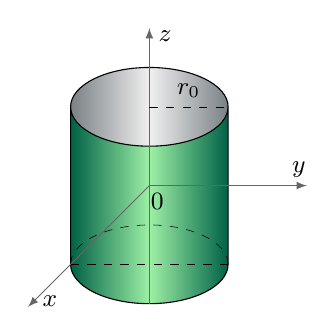
\begin{tikzpicture}
  \usetikzlibrary{arrows}
  \definecolor{insideo}{HTML}{798084}
  \definecolor{insidei}{HTML}{F0F0F0}
  \definecolor{outer}{HTML}{006146}
  \definecolor{inner}{HTML}{9EF0A6}
  \shade [left color=insideo,right color=insideo,middle color=insidei] (1,1) arc (0:180:1 and .5) --
   (-1,1) arc (180:360:1 and .5);
  \shadedraw [left color=outer,right color=outer,middle color=inner] (-1,-1) arc (180:360:1 and .5) -- (1,1) --
   (1,1) arc (360:180:1 and .5) -- (-1,-1);
  \draw (1,1) arc (0:180:1 and .5);
  \draw [dashed,line width=0.2pt] (1,-1) arc (0:180:1 and .5);
  \draw [black!60,line width=0.3pt,-latex] (0,0) -- (2,0,0);
  \draw [black!60,line width=0.3pt,-latex] (0,-1.5) -- (0,2,0);
  \draw [black!60,line width=0.3pt,-latex] (0,0) -- (0,0,4);
  \pgfputat{\pgfpointxyz{1.9}{0.2}{0}}{\pgfbox[center,center]{\small $y$}};
  \pgfputat{\pgfpointxyz{0.2}{1.9}{0}}{\pgfbox[center,center]{\small $z$}};
  \pgfputat{\pgfpointxyz{0.2}{0}{3.8}}{\pgfbox[center,center]{\small $x$}};
  \pgfputat{\pgfpointxyz{0.1}{-0.2}{0}}{\pgfbox[center,center]{\small $0$}};
  \draw [dashed,line width=0.2pt] (0,1) -- (1,1);
  \draw [dashed,line width=0.2pt] (-1,-1) -- (1,-1);
  \node [above] at (0.5,1) {\small $r_0$};
 \end{tikzpicture}
 &
 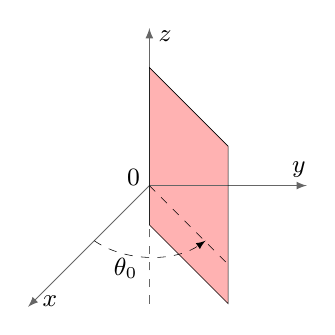
\begin{tikzpicture}
  \usetikzlibrary{arrows}
  \fill [red!30] (0,-.5) -- (1,-1.5) -- (1,.5) -- (0,1.5) -- (0,-.5);
  \draw [black!60,line width=0.3pt,-latex] (0,0) -- (2,0,0);
  \draw [black!60,line width=0.3pt,-latex] (0,-.5) -- (0,2,0);
  \draw [black!60,dashed,line width=0.3pt] (0,-1.5) -- (0,-.5);
  \draw [black!60,line width=0.3pt,-latex] (0,0) -- (0,0,4);
  \pgfputat{\pgfpointxyz{1.9}{0.2}{0}}{\pgfbox[center,center]{\small $y$}};
  \pgfputat{\pgfpointxyz{0.2}{1.9}{0}}{\pgfbox[center,center]{\small $z$}};
  \pgfputat{\pgfpointxyz{0.2}{0}{3.8}}{\pgfbox[center,center]{\small $x$}};
  \pgfputat{\pgfpointxyz{-0.2}{0.1}{0}}{\pgfbox[center,center]{\small $0$}};
  \draw [line width=0.2pt] (0,-.5) -- (1,-1.5) -- (1,.5) -- (0,1.5) -- (0,-.5);
  \draw [dashed,line width=0.2pt] (0,0) -- (1,-1);
  \draw [dashed,line width=0.2pt,-latex] (-0.7,-0.7) arc (225:315:1 and .7);
  \node [below] at (-0.3,-.8) {\small $\theta_0$};
 \end{tikzpicture}
 &
 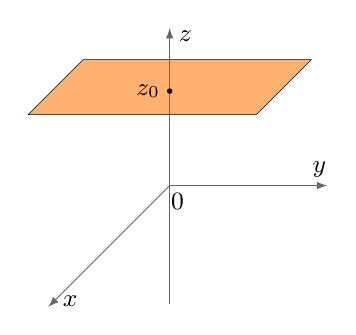
\begin{tikzpicture}
  \usetikzlibrary{arrows}
  \definecolor{planecolor}{HTML}{FFB270}
  \fill [planecolor] (-1.8,.9) -- (-1.1,1.6) -- (1.8,1.6) -- (1.1,.9) -- (-1.8,.9);
  \draw [line width=0.2pt] (-1.8,.9) -- (-1.1,1.6) -- (1.8,1.6) -- (1.1,.9) -- (-1.8,.9);
  \draw [black!60,line width=0.3pt,-latex] (0,0) -- (2,0,0);
  \draw [black!60,line width=0.3pt,-latex] (0,-1.5) -- (0,2,0);
  \draw [black!60,line width=0.3pt,-latex] (0,0) -- (0,0,4);
  \pgfputat{\pgfpointxyz{1.9}{0.2}{0}}{\pgfbox[center,center]{\small $y$}};
  \pgfputat{\pgfpointxyz{0.2}{1.9}{0}}{\pgfbox[center,center]{\small $z$}};
  \pgfputat{\pgfpointxyz{0.2}{0}{3.8}}{\pgfbox[center,center]{\small $x$}};
  \pgfputat{\pgfpointxyz{0.1}{-0.2}{0}}{\pgfbox[center,center]{\small $0$}};
  \fill (0,1.2) circle (1pt);
  \node [left] at (0,1.2) {\small $z_0$};
 \end{tikzpicture} \\
 (a) $r = r_0$ & (b) $\theta = \theta_0$ & (c) $z = z_0$
 \end{tabular}}
 \caption{Cylindrical coordinate surfaces}
 \label{fig:cylcoordsurf}
\end{lxfigure}

For spherical coordinates $(\rho,\theta,\phi)$, and constants $\rho_0$, $\theta_0$ and $\phi_0$, we see from \autoref{fig:sphcoordsurf} that the surface $\rho = \rho_0$ is a sphere of radius $\rho_0$ centered at the origin, the surface $\theta = \theta_0$ is a half-plane emanating from the $z$-axis, and the surface $\phi = \phi_0$ is a circular cone whose vertex is at the origin.

\begin{lxfigure}
 \flushinner{%
 \begin{tabular}{ccc}
 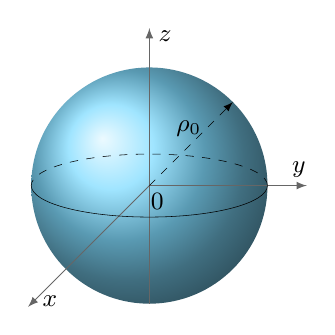
\begin{tikzpicture}
  \usetikzlibrary{arrows}
  \definecolor{spherecolor}{HTML}{80DCFF}
  \shade [ball color=spherecolor] (0,0) circle (1.5);
  \draw [black!60,line width=0.3pt,-latex] (0,0) -- (2,0,0);
  \draw [black!60,line width=0.3pt,-latex] (0,-1.5) -- (0,2,0);
  \draw [black!60,line width=0.3pt,-latex] (0,0) -- (0,0,4);
  \pgfputat{\pgfpointxyz{1.9}{0.2}{0}}{\pgfbox[center,center]{\small $y$}};
  \pgfputat{\pgfpointxyz{0.2}{1.9}{0}}{\pgfbox[center,center]{\small $z$}};
  \pgfputat{\pgfpointxyz{0.2}{0}{3.8}}{\pgfbox[center,center]{\small $x$}};
  \pgfputat{\pgfpointxyz{0.1}{-0.2}{0}}{\pgfbox[center,center]{\small $0$}};
  \draw [line width=0.2pt] (-1.5,0) arc (180:360:1.5 and 0.4);
  \draw [dashed,line width=0.2pt] (1.5,0) arc (0:180:1.5 and 0.4);
  \draw [dashed,line width=0.2pt,-latex] (0,0) -- (1.06,1.06);
  \node [above] at (0.5,0.5) {\small $\rho_0$};
 \end{tikzpicture}
 &
 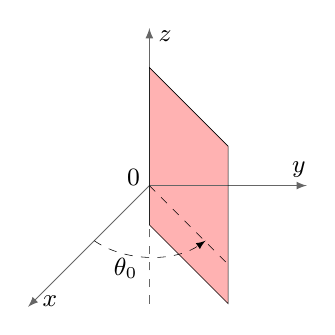
\begin{tikzpicture}
  \usetikzlibrary{arrows}
  \fill [red!30] (0,-.5) -- (1,-1.5) -- (1,.5) -- (0,1.5) -- (0,-.5);
  \draw [black!60,line width=0.3pt,-latex] (0,0) -- (2,0,0);
  \draw [black!60,line width=0.3pt,-latex] (0,-.5) -- (0,2,0);
  \draw [black!60,dashed,line width=0.3pt] (0,-1.5) -- (0,-.5);
  \draw [black!60,line width=0.3pt,-latex] (0,0) -- (0,0,4);
  \pgfputat{\pgfpointxyz{1.9}{0.2}{0}}{\pgfbox[center,center]{\small $y$}};
  \pgfputat{\pgfpointxyz{0.2}{1.9}{0}}{\pgfbox[center,center]{\small $z$}};
  \pgfputat{\pgfpointxyz{0.2}{0}{3.8}}{\pgfbox[center,center]{\small $x$}};
  \pgfputat{\pgfpointxyz{-0.2}{0.1}{0}}{\pgfbox[center,center]{\small $0$}};
  \draw [line width=0.2pt] (0,-.5) -- (1,-1.5) -- (1,.5) -- (0,1.5) -- (0,-.5);
  \draw [dashed,line width=0.2pt] (0,0) -- (1,-1);
  \draw [dashed,line width=0.2pt,-latex] (-0.7,-0.7) arc (225:315:1 and .7);
  \node [below] at (-0.3,-.8) {\small $\theta_0$};
 \end{tikzpicture}
 &
 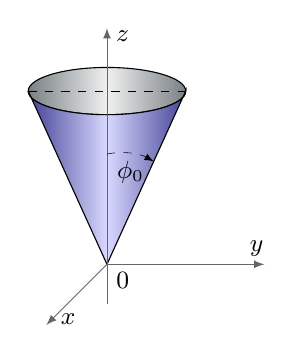
\begin{tikzpicture}
  \usetikzlibrary{arrows}
  \definecolor{insideo}{HTML}{798084}
  \definecolor{insidei}{HTML}{F0F0F0}
  \definecolor{outer}{HTML}{424296}
  \definecolor{inner}{HTML}{D8D8FF}
  \shadedraw [left color=insideo,right color=insideo,middle color=insidei] (1,2.2) arc (0:180:1 and .3) --
   (-1,2.2) arc (180:360:1 and .3);
  \shadedraw [left color=outer,right color=outer,middle color=inner] (-1,2.2) arc (180:360:1 and .3) -- (0,0) --
   (-1,2.2);
  \draw [black!60,line width=0.3pt,-latex] (0,0) -- (2,0,0);
  \draw [black!60,line width=0.3pt,-latex] (0,-.5) -- (0,3,0);
  \draw [black!60,line width=0.3pt,-latex] (0,0) -- (0,0,2);
  \pgfputat{\pgfpointxyz{1.9}{0.2}{0}}{\pgfbox[center,center]{\small $y$}};
  \pgfputat{\pgfpointxyz{0.2}{2.9}{0}}{\pgfbox[center,center]{\small $z$}};
  \pgfputat{\pgfpointxyz{0.2}{0}{1.8}}{\pgfbox[center,center]{\small $x$}};
  \pgfputat{\pgfpointxyz{0.2}{-0.2}{0}}{\pgfbox[center,center]{\small $0$}};
  \draw [dashed,line width=0.2pt] (-1,2.2) -- (1,2.2);
  \draw [dashed,line width=0.2pt,-latex] (0,1.4) arc (100:65:1 and 1.2);
  \node [above] at (0.3,0.9) {\small $\phi_0$};
 \end{tikzpicture} \\
  (a) $\rho = \rho_0$ & (b) $\theta = \theta_0$ & (c) $\phi = \phi_0$
  \end{tabular}}
 \caption{Spherical coordinate surfaces}
 \label{fig:sphcoordsurf}
\end{lxfigure}

Figures \ref{fig:cylcoordsurf}(a) and \ref{fig:sphcoordsurf}(a) show how these coordinate systems got their names.

Sometimes the equation of a surface in Cartesian coordinates can be transformed into a simpler equation in some other coordinate system, as in the following example.

\example{ex_conv_coord_eq}{Converting an Equation in Coordinate Systems}{Write the equation of the cylinder $x^2 + y^2 = 4$ in cylindrical coordinates.}{Since $r = \sqrt{x^2 + y^2}$, then the equation in cylindrical coordinates is $r =2$.}

Using spherical coordinates to write the equation of a sphere does not necessarily make the equation simpler, if the sphere is not centered at the origin.

\example{ex_bad_sphere}{Converting an Equation to Spherical Coordinates}{Write the equation $(x-2)^2+(y-1)^2+z^2=9$ in spherical coordinates.}{Multiplying the equation out gives
 \begin{align*}
  x^2+y^2+z^2-4x-2y+5 &= 9 \text{ , so we get} \\
  \rho^2-4\rho\sin\phi\cos\theta-2\rho\sin\phi\sin\theta-4 &= 0 \text{ , or}\\
  \rho^2-2\sin\phi(2\cos\theta-\sin\theta)\rho-4 &= 0
 \end{align*}
 after combining terms. Note that this actually makes it more difficult to figure out what the surface is, as opposed to the Cartesian equation where you could immediately identify the surface as a sphere of radius $3$ centered at $(2,1,0)$.}

\example{exmp_helicoid}{Identifying a Surface}{Describe the surface given by $\theta = z$ in cylindrical coordinates.}{This surface is called a \emph{helicoid}\index{helicoid}. As the (vertical) $z$ coordinate increases, so does the angle $\theta$, while the radius $r$ is unrestricted. So this sweeps out a (ruled!) surface shaped like a spiral staircase, where the spiral has an infinite radius. \autoref{fig:helicoid} shows a section of this surface restricted to $0 \le z \le 4\pi$ and $0 \le r \le 2$.
 \begin{lxfigure}
  \begin{center}
   \begin{tikzpicture}[scale=1.3]
    \begin{axis}[width=\textwidth,tick label style={font=\scriptsize},axis on top,
				axis lines=center,y dir=reverse,name=myplot,
				ymin=-2,ymax=2,xmin=-2,xmax=2,zmin=0,zmax=14]
     \addplot3[domain=0:2,y domain=0:720,surf,colormap={mp2}{\colormapplaneone},
		opacity=.6,faceted color=black!40,samples=8,samples y=72,very thin,
		z buffer=sort]
		({x*sin(y)},{x*cos(y)},{rad(y)});
    \end{axis}
    \node [left] at (myplot.below origin) [shift={(-60pt,0pt)}] {$x$};
    \node [below left] at (myplot.right of origin) [shift={(-30pt,-16pt)}] {$y$};
    \node [below] at (myplot.above origin) [shift={(0,-40pt)}] {$z$};
   \end{tikzpicture}
  \end{center}
 \caption{Helicoid $\theta = z$}\eoehere
 \label{fig:helicoid}
 \end{lxfigure}}

\printexercises{exercises/10_Other_Systems_exercises}



\apexchapter{Vector Valued Functions}{chap:vvf}

In the previous chapter, we learned about vectors and were introduced to the power of vectors within mathematics. In this chapter, we'll build on this foundation to define functions whose input is a real number and whose output is a vector. We'll see how to graph these functions and apply calculus techniques to analyze their behavior. Most importantly, we'll see \textit{why} we are interested in doing this: we'll see beautiful applications to the study of moving objects.

\section{Vector-Valued Functions}\label{sec:vvf}

% todo state how this compares with 10.2 & 10.3

We are very familiar with \textbf{real valued functions}, that is, functions whose output is a real number. This section introduces \textbf{vector-valued functions} --- functions whose output is a vector.

\begin{definition}[Vector-Valued Functions]\label{def:vvf}
A \textbf{vector-valued function} is a function of the form 
\[\vec r(t) =\bracket{\, f(t),g(t)\,}\quad \text{or}\quad \vec r(t) =\bracket{\,f(t),g(t),h(t)\,},\]
where $f$, $g$ and $h$ are real valued functions.\bigskip

The \textbf{domain} of $\vec r$ is the set of all values of $t$ for which $\vec r(t)$ is defined. The \textbf{range} of $\vec r$ is the set of all possible output vectors $\vec r(t)$.
\index{vector-valued function!definition}\index{function!vector-valued}
\end{definition}

\subsection{Evaluating and Graphing Vector-Valued Functions}

\mtable[-1in]{Sketching the graph of a vector-valued function.}{fig:vvfintro1}{%
\begin{tikzpicture}[>=stealth]
\begin{axis}[width=1.16\marginparwidth,tick label style={font=\scriptsize},
axis y line=middle,axis x line=middle,name=myplot,xtick={1,2,3,4,5},
ytick={-3,-2,-1,1,2,3},ymin=-3.5,ymax=3.5,xmin=-.5,xmax=5.5]
\draw [->,thick,draw={\colortwo}] (axis cs: 0,0) -- (axis cs:4,1)
 node [black,pos=.5,above] {\scriptsize $\vec r(-2)$};
\end{axis}
\node [right] at (myplot.right of origin) {\scriptsize $x$};
\node [above] at (myplot.above origin) {\scriptsize $y$};
\end{tikzpicture}
\\(a)\\
\begin{tikzpicture}[>=stealth]
\begin{axis}[width=1.16\marginparwidth,tick label style={font=\scriptsize},
axis y line=middle,axis x line=middle,name=myplot,xtick={1,2,3,4,5},
ytick={-3,-2,-1,1,2,3},ymin=-3.5,ymax=3.5,xmin=-.5,xmax=5.5]
\addplot [thick,draw={\colorone}, smooth,domain=-2.5:2.5] ({x^2},{x^2+x-1});
\draw [->,thick,] (axis cs:1,-1)--(axis cs: 0.9025,-1.0475);
\draw [->,thick,draw={\colortwo}] (axis cs: 0,0) -- (axis cs:4,1)
 node[black,pos=.5,above] {\scriptsize $\vec r(-2)$};
\end{axis}
\node [right] at (myplot.right of origin) {\scriptsize $x$};
\node [above] at (myplot.above origin) {\scriptsize $y$};
\end{tikzpicture}
\\(b)}

Evaluating a vector-valued function at a specific value of $t$ is straightforward; simply evaluate each component function at that value of $t$. For instance, if $\vec r(t) =\bracket{t^2,t^2+t-1}$, then $\vec r(-2) =\bracket{4,1}$. We can sketch this vector, as is done in \autoref{fig:vvfintro1}(a). Plotting lots of vectors is cumbersome, though, so generally we do not sketch the whole vector but just the terminal point. The \textbf{graph} of a vector-valued function is the set of all terminal points of $\vec r(t)$, where the initial point of each vector is always the origin. In \autoref{fig:vvfintro1}(b) we sketch the graph of $\vec r$\,; we can indicate individual points on the graph with their respective vector, as shown.
\index{vector-valued function!graphing}

Vector-valued functions are closely related to parametric equations. While in both methods we plot points $\bigl(x(t), y(t)\bigr)$ or $\bigl(x(t),y(t),z(t)\bigr)$ to produce a graph, in the context of vector-valued functions each such point represents a vector. The implications of this will be more fully realized in the next section as we apply calculus ideas to these functions.

\youtubeVideo{Djtttm0C7zA}{Domain of a Vector-Valued Function}

\mtable[-\baselineskip]{Sketching the vector-valued function of \autoref{ex_vvf1}.}{fig:vvf1}{%
\begin{tabular}{ c c c }
	$t$ & $t^3-t$ & $\ds \frac{1}{t^2+1}$ \\[6pt] \midrule
	$-2$&$-6$& 1/5\\  $-1$&0&1/2\\ 0&0&1\\ 1&0&1/2 \\ 2&6&1/5		
\end{tabular}
\\(a)\\[10pt]
\begin{tikzpicture}[>=stealth]
\begin{axis}[width=1.16\marginparwidth,tick label style={font=\scriptsize},
axis y line=middle,axis x line=middle,name=myplot,xtick={-6,-4,-2,2,4,6},
ymin=-.1,ymax=1.1,xmin=-7,xmax=7]
\addplot [thick,draw={\colorone}, smooth,domain=-2:2] ({x^3-x},{1/(x^2+1)});
\filldraw [black] (axis cs: -6,.2) circle (1.5pt);
\filldraw [black] (axis cs: 6,.2) circle (1.5pt);
\filldraw [black] (axis cs: 0,.5) circle (1.5pt);
\filldraw [black] (axis cs: 0.,1) circle (1.5pt);
\draw [->,thick,draw={\colortwo}] (axis cs:0,0)--(axis cs: 0,.5)
 node [,black,pos=.4,rotate=90,above] {\scriptsize $\vec r(-1)$};
\draw [->,thick,draw={\colortwo}] (axis cs:0,0)--(axis cs: 6,.2)
 node [black,pos=.4,above] {\scriptsize $\vec r(2)$};
\end{axis}
\node [right] at (myplot.right of origin) {\scriptsize $x$};
\node [above] at (myplot.above origin) {\scriptsize $y$};
\end{tikzpicture}
\\(b)}

\begin{example}[Graphing vector-valued functions]\label{ex_vvf1}
Graph $\ds \vec r(t) =\bracket{t^3-t, \frac{1}{t^2+1}}$, for $-2\leq t\leq 2$. Sketch $\vec r(-1)$ and $\vec r(2)$.
\solution
We start by making a table of $t$, $x$ and $y$ values as shown in \autoref{fig:vvf1}(a). Plotting these points gives an indication of what the graph looks like. In \autoref{fig:vvf1}(b), we indicate these points and sketch the full graph. We also highlight $\vec r(-1)$ and $\vec r(2)$ on the graph.
\end{example}

\begin{example}[Graphing vector-valued functions.]\label{ex_vvf2}
Graph $\vec r(t) =\bracket{\cos t,\sin t,t}$ for $0\leq t\leq 4\pi$.
\solution
We can again plot points, but careful consideration of this function is very revealing. Momentarily ignoring the third component, we see the $x$ and $y$ components trace out a circle of radius 1 centered at the origin. Noticing that the $z$ component is $t$, we see that as the graph winds around the $z$-axis, it is also increasing at a constant rate in the positive $z$ direction, forming a spiral. This is graphed in \autoref{fig:vvf2}. In the graph $\vec r(7\pi/4)=\bracket{\frac1{\sqrt2},-\frac1{\sqrt2},\frac{7\pi}4}%\approx \bracket{0.707,-0.707,5.498}
$ is highlighted to help us understand the graph.
\end{example}

\mtable[-.5in]{Viewing a vector-valued function, and its value at one point.}{fig:vvf2}{\myincludeasythree{width=\marginparwidth,
3Droll=1.5110919487882861,
3Dortho=0.0044999998062849045,
3Dc2c=0.6482614874839783 0.682218074798584 0.338135302066803,
3Dcoo=1.5296688079833984 -8.776086807250977 69.70178985595703,
3Droo=399.99999354879714}{width=\marginparwidth}{figures/figvvf2_3D}}

%\subsection{Algebra of Vector-Valued Functions}
%
%\begin{definition}[Operations on Vector-Valued Functions]\label{def:vvf_algebra}
%Let $\vec r_1(t)=\bracket{f_1(t),g_1(t)}$ and $\vec r_2(t)=\bracket{f_2(t),g_2(t)}$ be vector-valued functions in $\mathbb{R}^2$ and let $c$ be a scalar. Then:
%\begin{enumerate}
%	\item $\vec r_1(t) \pm \vec r_2(t) =\bracket{\, f_1(t)\pm f_2(t),g_1(t)\pm g_2(t)\,}$.
%	\item	$c\vec r_1(t) =\bracket{\, cf_1(t),cg_1(t)\,}$.
%\end{enumerate}
%A similar definition holds for vector-valued functions in $\mathbb{R}^3$.
%\index{vector-valued function!algebra of}
%\end{definition}
%
%This definition states that we add, subtract and scale vector-valued functions component-wise. Combining vector-valued functions in this way can be very useful (as well as create interesting graphs).

\begin{example}[Adding and scaling vector-valued functions.]\label{ex_vvf3}
Let $\vec r_1(t) =\bracket{\,0.2t,0.3t\,}$, $\vec r_2(t) =\bracket{\,\cos t,\sin t\,}$ and $\vec r(t) = \vec r_1(t)+\vec r_2(t)$. Graph $\vec r_1(t)$, $\vec r_2(t)$, $\vec r(t)$ and $5\vec r(t)$ on $-10\leq t\leq10$.
\solution
We can graph $\vec r_1$ and $\vec r_2$ easily by plotting points (or just using technology). Let's think about each for a moment to better understand how vector-valued functions work.

We can rewrite $\vec r_1(t) =\bracket{\, 0.2t,0.3t\,}$ as $ \vec r_1(t) = t\bracket{0.2,0.3}$. That is, the function $\vec r_1$ scales the vector $\bracket{0.2,0.3}$ by $t$. This scaling of a vector produces a line in the direction of $\bracket{0.2,0.3}$.

We are familiar with $\vec r_2(t) =\bracket{\, \cos t,\sin t\,}$; it traces out a circle, centered at the origin, of radius 1. \autoref{fig:vvf3}(a) graphs $\vec r_1(t)$ and $\vec r_2(t)$.

\mtable{Graphing the functions in \autoref{ex_vvf3}.}{fig:vvf3}{%
\begin{tikzpicture}[>=stealth]
\begin{axis}[width=1.16\marginparwidth,tick label style={font=\scriptsize},
axis y line=middle,axis x line=middle,name=myplot,
ymin=-4.1,ymax=4.1,xmin=-4.9,xmax=4.9]
\addplot [thick,draw={\colorone}, smooth,domain=-10:10] ({.2*x},{.3*x});
\draw[thick,draw={\colorone},smooth](axis cs:0,0)circle(1);
%\addplot [thick,draw={\colorone}, smooth,domain=0:360] ({cos(x)},{sin(x)});
\end{axis}
\node [right] at (myplot.right of origin) {\scriptsize $x$};
\node [above] at (myplot.above origin) {\scriptsize $y$};
\end{tikzpicture}
\\(a)\\[10pt]
\begin{tikzpicture}[>=stealth]
\begin{axis}[width=1.16\marginparwidth,tick label style={font=\scriptsize},
axis y line=middle,axis x line=middle,name=myplot,
ymin=-4.1,ymax=4.1,xmin=-4.9,xmax=4.9]
\addplot [thick,draw={\colorone}, smooth,domain=-10:10,samples=60]
 ({.2*x+cos(deg(x))},{.3*x+sin(deg(x))});
\end{axis}
\node [right] at (myplot.right of origin) {\scriptsize $x$};
\node [above] at (myplot.above origin) {\scriptsize $y$};
\end{tikzpicture}
\\(b)\\[10pt]
\begin{tikzpicture}[>=stealth]
\begin{axis}[width=1.16\marginparwidth,tick label style={font=\scriptsize},
axis y line=middle,axis x line=middle,name=myplot,xtick={-20,-10,10,20},
ymin=-20.5,ymax=20.5,xmin=-24.5,xmax=24.5]
\addplot [thick,draw={\colorone}, smooth,domain=-10:10,samples=60]
 ({.2*x+cos(deg(x))},{.3*x+sin(deg(x))});
\addplot [thick,draw={\colorone}, smooth,domain=-10:10,samples=60]
 ({x+5*cos(deg(x))},{1.5*x+5*sin(deg(x))});
\end{axis}
\node [right] at (myplot.right of origin) {\scriptsize $x$};
\node [above] at (myplot.above origin) {\scriptsize $y$};
\end{tikzpicture}
\\(c)}

Adding $\vec r_1(t)$ to $\vec r_2(t)$ produces $\vec r(t) =\bracket{\,\cos t + 0.2t,\sin t+0.3t\,}$, graphed in \autoref{fig:vvf3}(b). The linear movement of the line combines with the circle to create loops that move in the direction of $\bracket{0.2,0.3}$.  (We encourage the reader to experiment by changing $\vec r_1(t)$ to $\bracket{2t,3t}$, etc., and observe the effects on the loops.)

Multiplying $\vec r(t)$ by 5 scales the function by 5, producing
\[5\vec r(t) =\bracket{5\cos t+t,5\sin t+\frac32t},\]
which is graphed in \autoref{fig:vvf3}(c) along with $\vec r(t)$. The new function is ``5 times bigger'' than $\vec r(t)$. Note how the graph of $5\vec r(t)$ in (c) looks identical to the graph of $\vec r(t)$ in $(b)$. This is due to the fact that the $x$ and $y$ bounds of the plot in $(c)$ are exactly 5 times larger than the bounds in (b).
\end{example}

\begin{example}[Adding and scaling vector-valued functions.]\label{ex_vvf4}
A \textbf{cycloid} is a graph traced by a point $p$ on a rolling circle, as shown in \autoref{fig:vvf4}. Find an equation describing the cycloid, where the circle has radius 1.
\index{cycloid}
{\centering
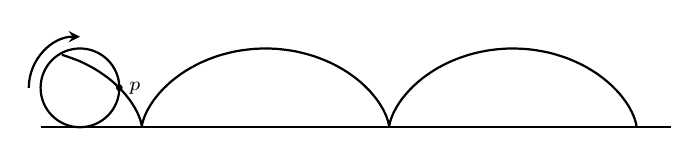
\begin{tikzpicture}[>=stealth,scale=.5]
\draw [thick] (0,1) circle (1);
\filldraw (1,1) circle (2pt) node [right] {\scriptsize $p$};
\draw [draw={\colorone},thick,domain=-1:14,smooth,samples=60]
 plot ({cos(\x r)+\x},{-sin(\x r)+1});
\draw [thick] (-1,0) -- (15,0);
\draw [thick,->] (-1.3,1) arc (180:90:1.3);
\draw [thick,white] (0,2.5) -- (1,2.5);
\end{tikzpicture}
\captionsetup{type=figure}
\caption{Tracing a cycloid.}\label{fig:vvf4}
}% end centering
\solution
This problem is not very difficult if we approach it in a clever way. We start by letting $\vec p(t)$ describe the position of the point $p$ on the circle, where the circle is centered at the origin and only rotates clockwise (i.e., it  does not roll). This is relatively simple given our previous experiences with parametric equations; $\vec p(t) =\bracket{\cos t, -\sin t}$. 

We now want the circle to roll. We represent this by letting $\vec c(t)$ represent the location of the center of the circle. It should be clear that the $y$ component of $\vec c(t)$ should be 1; the center of the circle is always going to be 1 if it rolls on a horizontal surface.

%% to do how does this differ from the previous figure?
%\mtable{The cycloid in \autoref{ex_vvf4}.}{fig:vvfa}{\begin{tikzpicture}[>=stealth]
%\begin{axis}[width=1.16\marginparwidth,tick label style={font=\scriptsize},
%axis y line=middle,axis x line=middle,name=myplot,
%ymin=-.1,ymax=14,xmin=-.5,xmax=16]
%\addplot [thick,draw={\colorone}, smooth,domain=-1:16,samples=60]
% ({cos(deg(x))+x},{-sin(deg(x))+1});
%\end{axis}
%\node [right] at (myplot.right of origin) {\scriptsize $x$};
%\node [above] at (myplot.above origin) {\scriptsize $y$};
%\end{tikzpicture}}

The $x$ component of $\vec c(t)$ is a linear function of $t$: $f(t) = mt$ for some scalar $m$. When $t=0$, $f(t) = 0$ (the circle starts centered on the $y$-axis). When $t=2\pi$, the circle has made one complete revolution, traveling a distance equal to its circumference, which is also $2\pi$. This gives us a point on our line $f(t) = mt$, the point $(2\pi, 2\pi)$. It should be clear that $m=1$ and $f(t) = t$. So $\vec c(t) =\bracket{t, 1}$. 

We now combine $\vec p$ and $\vec c$ together to form the equation of the cycloid: $\vec r(t) = \vec p(t) + \vec c(t) =\bracket{\cos t+ t,-\sin t+1}$, which
matches the graph in \autoref{fig:vvf4}.
% is graphed in \autoref{fig:vvfa}.
\end{example}

\subsection{Displacement}

A vector-valued function $\vec r(t)$ is often used to describe the position of a moving object at time $t$. At $t=t_0$, the object is at $\vec r(t_0)$; at $t=t_1$, the object is at $\vec r(t_1)$. Knowing the locations $\vec r(t_0)$ and $\vec r(t_1)$ give no indication of the path taken between them, but often we only care about the difference of the locations, $\vec r(t_1)-\vec r(t_0)$, the \textbf{displacement}.\index{displacement}\index{vector-valued function!displacement}

\begin{definition}[Displacement]\label{def:displacement}
Let $\vec r(t)$ be a vector-valued function and let $t_0<t_1$ be values in the domain. The \textbf{displacement} $\vec d$ of $\vec r$, from $t=t_0$ to $t=t_1$, is \[\vec d=\vec r(t_1)-\vec r(t_0).\]
\end{definition}

When the displacement vector is drawn with initial point at $\vec r(t_0)$, its terminal point is $\vec r(t_1)$. We think of it as the vector which points from a starting position to an ending position.

\begin{example}[Finding and graphing displacement vectors]\label{ex_vvf5}
Let $\vec r(t) =\bracket{\cos (\frac{\pi}{2}t),\sin (\frac{\pi}2 t)}$. Graph $\vec r(t)$ on $-1\leq t\leq 1$, and find the displacement of $\vec r(t)$ on this interval.
\solution
The function $\vec r(t)$ traces out the unit circle, though at a different rate than the ``usual'' $\bracket{\cos t,\sin t}$ parameterization. At $t_0=-1$, we have $\vec r(t_0) =\bracket{0,-1}$; at $t_1=1$, we have $\vec r(t_1) =\bracket{0,1}$. The displacement of $\vec r(t)$ on $[-1,1]$ is thus $\vec d =\bracket{0,1}-\bracket{0,-1}=\bracket{0,2}.$

\mtable{Graphing the displacement of a position function in \autoref{ex_vvf5}.}{fig:vvf5}{\begin{tikzpicture}[>=stealth]
\begin{axis}[width=1.16\marginparwidth,tick label style={font=\scriptsize},
axis y line=middle,axis x line=middle,name=myplot,ytick={-1,1},
ymin=-1.1,ymax=1.1,xmin=-1.32,xmax=1.32]
\addplot [thick,draw={\colorone}, smooth,domain=-90:90,samples=20] ({cos(x)},{sin(x)});
\draw [thick,->,draw={\colortwo}] (axis cs: 0,-1) -- (axis cs:0,1)
 node [left,pos=.7,black]{\scriptsize $\vec d$};
\end{axis}
\node [right] at (myplot.right of origin) {\scriptsize $x$};
\node [above] at (myplot.above origin) {\scriptsize $y$};
\end{tikzpicture}}

A graph of $\vec r(t)$ on $[-1,1]$ is given in \autoref{fig:vvf5}, along with the displacement vector $\vec d$ on this interval.
\end{example}

Measuring displacement makes us contemplate related, yet very different, concepts. Considering the semi-circular path the object in \autoref{ex_vvf5} took, we can quickly verify that the object ended up a distance of 2 units from its initial location. That is, we can compute $\vnorm{d} = 2$. However, measuring \emph{distance from the starting point} is different from measuring \emph{distance traveled}. Being a semi-circle, we can measure the distance traveled by this object as $\pi%\approx 3.14
$ units. Knowing \emph{distance from the starting point} allows us to compute \textbf{average rate of change.}

\begin{definition}[Average Rate of Change]\label{def:av_rate_of_change_vect}
Let $\vec r(t)$ be a vector-valued function, where each of its component functions is continuous on its domain, and let $t_0<t_1$. The \textbf{average rate of change} of $\vec r(t)$ on $[t_0,t_1]$ is
\index{average rate of change}\index{vector-valued function!average rate of change}
\[\text{average rate of change} = \frac{\vec r(t_1) - \vec r(t_0)}{t_1-t_0}.\]
\end{definition}

\begin{example}[Average rate of change]\label{ex_vvf6}
Let $\vec r(t) =\bracket{\cos(\frac{\pi}2t),\sin(\frac{\pi}2t)}$ as in \autoref{ex_vvf5}. Find the average rate of change of $\vec r(t)$ on $[-1,1]$ and on $[-1,5]$.
\solution
We computed in \autoref{ex_vvf5} that the displacement of $\vec r(t)$ on $[-1,1]$ was $\vec d =\bracket{0,2}$. Thus the average rate of change of $\vec r(t)$ on $[-1,1]$ is:
\[\frac{\vec r(1) -\vec r(-1)}{1-(-1)} = \frac{\bracket{0,2}}{2} =\bracket{0,1}.\]
We interpret this as follows: the object followed a semi-circular path, meaning it moved towards the right then moved back to the left, while climbing slowly, then quickly, then slowly again. \emph{On average}, however, it progressed straight up at a constant rate of $\bracket{0,1}$ per unit of time.

We can quickly see that the displacement on $[-1,5]$ is the same as on $[-1,1]$, so $\vec d =\bracket{0,2}$. The average rate of change is different, though:
\[\frac{\vec r(5)-\vec r(-1)}{5-(-1)} = \frac{\bracket{0,2}}{6} =\bracket{0,1/3}.\]
As it took ``3 times as long'' to arrive at the same place, this average rate of change on $[-1,5]$ is $1/3$ the average rate of change on $[-1,1]$.
\end{example}

We considered average rates of change in Sections \ref{sec:limit_intro} and \ref{sec:derivative} as we studied limits and derivatives. The same is true here; in the following section we apply calculus concepts to vector-valued functions as we find limits, derivatives, and integrals. Understanding the average rate of change will give us an understanding of the derivative; displacement gives us one application of integration.

\printexercises{exercises/11-01-exercises}

\section{Calculus and Vector-Valued Functions}\label{sec:vvf_calc}

The previous section introduced us to a new mathematical object, the vector-valued function. We now apply calculus concepts to these functions. We start with the limit, then work our way through derivatives to integrals.

\subsection{Limits of Vector-Valued Functions}

The initial definition of the limit of a vector-valued function is a bit intimidating, as was the definition of the limit in \autoref{def:limit}. The theorem following the definition shows that in practice, taking limits of vector-valued functions is no more difficult than taking limits of real-valued functions.

\begin{definition}[Limits of Vector-Valued Functions]\label{def:vvf_limit}
Let $I$ be an open interval containing $c$, and let $\vec r(t)$ be a vector-valued function defined on $I$, except possibly at $c$. %Let a vector-valued function $\vec r(t)$ be given, defined on an open interval $I$ containing $c$. 
The \textbf{limit of $\vec r(t)$, as $t$ approaches $c$, is $\vec L$}, expressed as 
\[\lim_{t\to c} \vec r(t) = \vec L,\]
means that given any $\epsilon>0$, there exists a $\delta>0$ such that for all $t\neq c$, if $\abs{t-c}<\delta$, we have $\norm{\vec r(t) - \vec L} < \epsilon.$
\index{vector-valued function!limits}\index{limit!of vector-valued functions}
\end{definition}

Note how the measurement of distance between real numbers is the absolute value of their difference; the measure of distance between vectors is the vector norm, or magnitude, of their difference.

\begin{theorem}[Limits of Vector-Valued Functions]\label{thm:vvf_limit}
\index{vector-valued function!limits}\index{limit!of vector-valued functions}%
\mbox{}\\[-2\baselineskip]\begin{enumerate}
	\item Let $\vec r(t) =\bracket{\,f(t),g(t)\,}$ be a vector-valued function in $\mathbb{R}^2$ defined on an open interval $I$ containing $c$. Then
\[\lim_{t\to c} \vec r(t) =\bracket{\lim_{t\to c}f(t)\, , \,\lim_{t\to c} g(t)}.\]
	\item Let $\vec r(t) =\bracket{\,f(t),g(t),h(t)\,}$ be a vector-valued function in $\mathbb{R}^3$ defined on an open interval $I$ containing $c$. Then 
\[
\lim_{t\to c} \vec r(t)
=\bracket{\lim_{t\to c}f(t)\, , \,\lim_{t\to c} g(t)\,, \,\lim_{t\to c} h(t)}
\]
\end{enumerate}
If any of the component limits do not exist, then $\ds\lim_{t\to c} \vec r(t)$ does not exist.
\end{theorem}

\autoref{thm:vvf_limit} states that we compute limits component-wise.

\begin{example}[Finding limits of vector-valued functions]\label{ex_vvflimit1}
Let $\ds\vec r(t) =\bracket{\frac{\sin t}{t},\, t^2-3t+3,\,\cos t}.$ Find $\ds \lim_{t\to 0}\vec r(t)$.
\solution
We apply the theorem and compute limits component-wise.
\begin{align*}
\lim_{t\to0} \vec r(t) &=\bracket{\lim_{t\to 0}\frac{\sin t}{t}\, , \, \lim_{t\to 0} t^2-3t+3\, , \, \lim_{t\to 0} \cos t}\\
			&=\bracket{1,3,1}.
\end{align*}
\end{example}

\subsection{Continuity}

\begin{definition}[Continuity of Vector-Valued Functions]\label{def:vvf_continuity}
Let $\vec r(t)$ be a vector-valued function defined on an open interval $I$ containing $c$.
\index{vector-valued function!continuity}\index{continuous function!vector-valued}
\begin{enumerate}
	\item $\vec r(t)$ is \textbf{continuous at $c$} if $\ds \lim_{t\to c} \vec r(t) = \vec r(c)$.
	\item	If $\vec r(t)$ is continuous at all $c$ in $I$, then $\vec r(t)$ is \textbf{continuous on $I$.}
\end{enumerate}
\end{definition}

We again have a theorem that lets us evaluate continuity component-wise.

\begin{theorem}[Continuity of Vector-Valued Functions]\label{thm:vvf_continuity}
Let $\vec r(t)$ be a vector-valued function defined on an open interval $I$ containing $c$. Then $\vec r(t)$ is continuous at $c$ if, and only if, each of its component functions is continuous at $c$.
\index{vector-valued function!continuity}\index{continuous function!vector-valued}
\end{theorem}

\begin{example}[Evaluating continuity of vector-valued functions]\label{ex_vvflimit2}
Let $\ds\vec r(t) =\bracket{\frac{\sin t}{t},\, t^2-3t+3,\,\cos t}.$ Determine whether $\vec r$ is continuous at $t=0$ and $t=1$.
\solution
While the second and third components of $\vec r(t)$ are defined at $t=0$, the first component, $(\sin t)/t$, is not. Since the first component is not even defined at $t=0$, $\vec r(t)$ is not defined at $t=0$, and hence it is not continuous at $t=0$.

At $t=1$ each of the component functions is continuous. Therefore $\vec r(t)$ is continuous at $t=1$.
\end{example}

\subsection{Derivatives}

Consider a vector-valued function $\vec r$ defined on an open interval $I$ containing $t_0$ and $t_1$. We can compute the displacement of $\vec r$ on $[t_0,t_1]$, as shown in \autoref{fig:vvfderiv_intro}(a). Recall that dividing the displacement vector by $t_1-t_0$ gives the average rate of change on $[t_0,t_1]$, as shown in (b).

\noindent\begin{minipage}[t]{\linewidth}\noindent%
\captionsetup{type=figure}%
\flushinner{%
\begin{tabular}{cc}
\begin{tikzpicture}[>=stealth]
 \draw [thick,draw={\colorone}]
  (2,1) arc [x radius=4,y radius=3,start angle=145,end angle=135] node (A) {};
 \draw [thick,draw={\colorone}]
  (A.center) arc [x radius=4,y radius=3,start angle=135,end angle=70] node (B) {};
 \draw [thick,draw={\colorone}]
  (B.center) arc [x radius=4,y radius=3,start angle=70,end angle=60];
 \draw [thick,->] (0,0) -- (A.center) node [left,pos=.6] {\scriptsize $\vec r(t_0)$};
 \draw [thick,->] (0,0)
  -- (B.center) node [below,pos=.5] {\scriptsize $\vec r(t_1)$};
 \draw [->,thick,draw={\colortwo}] (A)
  --(B) node [above,black,pos=.5,sloped] {\scriptsize $\vec r(t_1)-\vec r(t_0)$};
\end{tikzpicture}
&
\begin{tikzpicture}[>=stealth]
 \draw [thick,draw={\colorone}]
  (2,1) arc [x radius=4,y radius=3,start angle=145,end angle=135] node (A) {};
 \draw [thick,draw={\colorone}]
  (A.center) arc [x radius=4,y radius=3,start angle=135,end angle=70] node (B) {};
 \draw [thick,draw={\colorone}]
  (B.center) arc [x radius=4,y radius=3,start angle=70,end angle=60];
 \draw [thick,->] (0,0) -- (A.center) node [left,pos=.6] {\scriptsize $\vec r(t_0)$};
 \draw [thick,->] (0,0)
  -- (B.center) node [below,pos=.5] {\scriptsize $\vec r(t_1)$};
 \draw [->,thick,draw={\colortwo}] (A.center)--($(A)!1.2!(B)$)
  node [above,black,pos=.99,] {$\frac{\vec r(t_1)-\vec r(t_0)}{t_1-t_0}$};
 \draw [->,thick,draw={\colortwo}] (A.center)--($(A)!.4!29:(B)$)
  node [above,black] {\scriptsize $\vec r\,'(t_0)$};
\end{tikzpicture}
\\(a) & (b)
\end{tabular}}
\caption{Illustrating displacement, leading to an understanding of the derivative of vector-valued functions.}
\label{fig:vvfderiv_intro}
\end{minipage}

The \textbf{derivative} of a vector-valued function is a measure of the \emph{instantaneous} rate of change, measured by taking the limit as the length of $[t_0,t_1]$ goes to 0. Instead of thinking of an interval as $[t_0,t_1]$, we think of it as $[c,c+h]$ for some value of $h$ (hence the interval has length $h$).  The \emph{average} rate of change is 
\[\frac{\vec r(c+h)-\vec r(c)}{h}\]
for any value of $h\neq0$. We take the limit as $h\to0$ to measure the instantaneous rate of change; this is the derivative of $\vec r$.

%We begin with a definition of the derivative that is very similar to \autoref{def:the_derivative}.

\begin{definition}[Derivative of a Vector-Valued Function]\label{def:vvf_derivative}
Let $\vec r(t)$ be continuous on an open interval $I$ containing $c$.
\index{vector-valued function!derivatives}\index{derivative!vector-valued functions}
\begin{enumerate}
	\item The derivative of $\vec r$ at $t=c$ is the vector
	\[\vrp (c) = \lim_{h\to 0} \frac{\vec r(c+h) - \vec r(c)}{h}.\]
	\item	The derivative of $\vec r$ is the vector-valued function
	\[\vrp (t) = \lim_{h\to 0} \frac{\vec r(t+h) - \vec r(t)}{h}.\]
\end{enumerate}
\end{definition}

\mnote{Alternate notations for the derivative of $\vec r$ include:
\[\vrp(t) = \frac{d}{dt}\bigl(\,\vec r(t)\,\bigr) = \frac{d\vec r}{dt}.\]}

If a vector-valued function has a derivative for all $c$ in an open interval $I$, we say that $\vec r(t)$ is \textbf{differentiable} on $I$.

Once again we might view this definition as intimidating, but recall that we can evaluate limits component-wise. The following theorem verifies that this means we can compute derivatives component-wise as well, making the task not too difficult.

\begin{theorem}[Derivatives of Vector-Valued Functions]\label{thm:vvf_deriv}
\index{vector-valued function!derivatives}\index{derivative!vector-valued functions}
\mbox{}\\[-2\baselineskip]\begin{enumerate}
	\item Let $\vec r(t) =\bracket{\, f(t), g(t)\,}$. Then 
	\[\vrp(t) =\bracket{\, \fp(t), g\primeskip'(t)\,}.\]
	\item Let $\vec r(t) =\bracket{\, f(t), g(t), h(t)\,}$. Then
	\[\vrp(t) =\bracket{\, \fp(t), g\primeskip'(t), h\primeskip'(t)\,}.\]
\end{enumerate}
If any of the component derivatives do not exist, then $\vrp(t)$ does not exist.
\end{theorem}

\youtubeVideo{238wiC0U7NE}{Limit and Derivative of Vector Function}

\mtable[-1in]{Graphing the derivative of a vector-valued function in \autoref{ex_vvflimit3}.}{fig:vvflimit3}{%
\begin{tikzpicture}[>=stealth]
\begin{axis}[width=1.16\marginparwidth,tick label style={font=\scriptsize},
axis y line=middle,axis x line=middle,name=myplot,
ymin=-2.2,ymax=2.2,xmin=-4.54,xmax=4.54]
\addplot [thick,draw={\colorone}, smooth,domain=-2:2,samples=20] ({x^2},{x});
\draw (axis cs:2,1.7) node {\scriptsize $\vec r(t)$};
\draw [thick,draw={\colortwo}] (axis cs: -4,1) -- (axis cs:4,1)
 node [below,pos=.9,black]{\scriptsize $\vec r\,'(t)$};
\draw [thick,draw={\colortwo},->] (axis cs: -2,1) -- (axis cs:-1.99,1);
\draw [thick,->,draw={\colorone}] (axis cs:1,-1) -- (axis cs:0.9801,-.99);
\end{axis}
\node [right] at (myplot.right of origin) {\scriptsize $x$};
\node [above] at (myplot.above origin) {\scriptsize $y$};
\end{tikzpicture}
\\[5pt](a)\\[10pt]
\begin{tikzpicture}[>=stealth]
\begin{axis}[width=1.16\marginparwidth,tick label style={font=\scriptsize},
axis y line=middle,axis x line=middle,name=myplot,
ymin=-2.2,ymax=2.2,xmin=-4.54,xmax=4.54]
\addplot [thick,draw={\colorone}, smooth,domain=-2:2,samples=20] ({x^2},{x});
\draw [thick,->,draw={\colortwo}] (axis cs: 0,0) -- (axis cs:2,1)
 node [shift={(15pt,0)},pos=.6,black]{\scriptsize $\vec r\,'(1)$};
\draw [thick,->,draw={\colortwo}] (axis cs: 1,1) -- (axis cs:3,2)
 node [left,pos=.8,black]{\scriptsize $\vec r\,'(1)$};
\draw [thick,->,draw={\colorone}] (axis cs:1,-1) -- (axis cs:0.9801,-.99);
\end{axis}
\node [right] at (myplot.right of origin) {\scriptsize $x$};
\node [above] at (myplot.above origin) {\scriptsize $y$};
\end{tikzpicture}
\\[5pt](b)}

\begin{example}[Derivatives of vector-valued functions]\label{ex_vvflimit3}
Let $\vec r(t) =\bracket{t^2,t}$. 
\begin{enumerate}
	\item Sketch $\vec r(t)$ and $\vrp(t)$ on the same axes.
	\item	Compute $\vrp(1)$ and sketch this vector with its initial point at the origin and at $\vec r(1)$.
\end{enumerate}
\solution
\begin{enumerate}
\item	\autoref{thm:vvf_deriv} allows us to compute derivatives component-wise, so
\[\vrp(t) =\bracket{2t, 1}.\]
$\vec r(t)$ and $\vrp(t)$ are graphed together in \autoref{fig:vvflimit3}(a). Note how plotting the two of these together, in this way, is not very illuminating. When dealing with real-valued functions, plotting $f(x)$ with $\fp(x)$ gave us useful information as we were able to compare $f$ and $\fp$ at the same $x$-values. When dealing with vector-valued functions, it is hard to tell which points on the graph of $\vrp$ correspond to which points on the graph of $\vec r$.

\item	We easily compute $\vrp(1) =\bracket{2,1}$, which is drawn in \autoref{fig:vvflimit3} with its initial point at the origin, as well as at $\vec r(1) =\bracket{1,1}.$ These are sketched in \autoref{fig:vvflimit3}(b).
\end{enumerate}
\end{example}

\ifthenelse{\boolean{in_threeD}}{%
\mtable{Viewing a vector-valued function and its derivative at one point.}{fig:vvflimit4}{%
\myincludeasythree{width=.7\marginparwidth,
3Droll=-0.5856992334166129,
3Dortho=0.004399999976158142,
3Dc2c=0.6354137063026428 0.6317671537399292 0.4439816176891327,
3Dcoo=-18.837804794311523 -8.740551948547363 60.22870635986328,
3Droo=150.0000027221829}{width=.7\marginparwidth}{figures/figvvflimit4_3D}}%
}{% not in threeD
\mtable[-3\baselineskip]{Viewing a vector-valued function and its derivative at one point, from two different perspectives.}{fig:vvflimit4}{%
\myincludegraphics[width=.7\marginparwidth]{figures/figvvflimit4_3D}
\\(a)\\
\myincludegraphics[width=.7\marginparwidth]{figures/figvvflimit4a_3D}
\\(b)}%
}% ends whole if-then-else

\begin{example}[Derivatives of vector-valued functions]\label{ex_vvflimit4}
Let $\vec r(t) =\bracket{\cos t, \sin t, t}$. Compute $\vrp(t)$ and $\vrp(\pi/2)$. Sketch $\vrp(\pi/2)$ with its initial point at the origin and at $\vec r(\pi/2)$.
\solution
We compute $\vrp$ as $\vrp(t) =\bracket{-\sin t, \cos t, 1}$. At $t= \pi/2$, we have $\vrp(\pi/2) =\bracket{-1,0,1}$. \autoref{fig:vvflimit4}
\ifthenelse{\boolean{in_threeD}}{shows a graph of $\vec r(t)$,}{shows two graphs of $\vec r(t)$, from different perspectives,}
with $\vrp(\pi/2)$ plotted with its initial point at the origin and at $\vec r(\pi/2)$.
\end{example}

In Examples \ref{ex_vvflimit3} and \ref{ex_vvflimit4}, sketching a particular derivative with its initial point at the origin did not seem to reveal anything significant. However, when we sketched the vector with its initial point on the corresponding point on the graph, we did see something significant: the vector appeared to be \emph{tangent} to the graph. We have not yet defined what ``tangent'' means in terms of curves in space; in fact, we use the derivative to define this term.

\begin{definition}[Tangent Vector, Tangent Line]\label{def:vector_tangent}
Let $\vec r(t)$ be a differentiable vector-valued function on an open interval $I$ containing $c$, where $\vrp(c)\neq \vec 0$.
\index{tangent line}\index{vector-valued function!tangent line}
\begin{enumerate}
	\item A vector $\vec v$ is \textbf{tangent to the graph of $\vec r(t)$ at $t=c$} if $\vec v$ is parallel to $\vrp(c)$.
	\item	The \textbf{tangent line}  to the graph of $\vec r(t)$ at $t=c$ is the line through $\vec r(c)$ with direction parallel to $\vrp(c)$. An equation of the tangent line is 
	\[\vec \ell(t) = \vec r(c) + t\,\vrp(c).\]
\end{enumerate}
\end{definition}

\begin{example}[Finding tangent lines to curves in space]\label{ex_vvfderiv1}
Let $\vec r(t) =\bracket{t,t^2,t^3}$ on $[-1.5,1.5]$. Find the vector equation of the line tangent to the graph of $\vec r$ at $t=-1$.
\solution
To find the equation of a line, we need a point on the line and the line's direction. The point is given by $\vec r(-1) =\bracket{-1,1,-1}$. (To be clear, $\bracket{-1,1,-1}$ is a \emph{vector}, not a point, but we use the point ``pointed to'' by this vector.)

\ifthenelse{\boolean{in_threeD}}{% in threeD
\mtable{Graphing a curve in space with its tangent line.}{fig:vvfderiv1}{%
\myincludeasythree{width=\marginparwidth,
3Droll=0.5961816528018784,
3Dortho=0.00514203542843461,
3Dc2c=0.8352102637290955 0.5152699947357178 0.19214747846126556,
3Dcoo=-5.658682346343994 19.23411750793457 0.2712952494621277,
3Droo=149.99999927774635}{width=\marginparwidth}{figures/figvvfderiv1_3D}}
}{% not in three D
\mtable{Graphing a curve in space with its tangent line.}{fig:vvfderiv1}{%
\myincludegraphics[width=\marginparwidth]{figures/figvvfderiv1_3D}
\\(a)\\[10pt]
\myincludegraphics[width=\marginparwidth]{figures/figvvfderiv1b_3D}
\\(b)}% end mtable
}% ends all of the if-then-else statements

The direction comes from $\vrp(-1)$. We compute, component-wise, $\vrp(t) =\bracket{1,2t, 3t^2}$. Thus $\vrp(-1) =\bracket{1,-2,3}$. 

The vector equation of the line is $\ell(t) =\bracket{-1,1,-1}+ t\bracket{1,-2,3}$. \ifthenelse{\boolean{in_threeD}}{This line and $\vec r(t)$ are sketched in \autoref{fig:vvfderiv1}.}{This line and $\vec r(t)$ are sketched, from two perspectives, in \autoref{fig:vvfderiv1} (a) and (b).}
\end{example}

\begin{example}[Finding tangent lines to curves]\label{ex_vvfderiv3}
Find the equations of the lines tangent to $\vec r(t) =\bracket{t^3,t^2}$ at $t=-1$ and $t=0$.
\solution
We find that $\vrp(t) =\bracket{3t^2,2t}$. At $t=-1$, we have
\[\vec r(-1) =\bracket{-1,1}\quad \text{and}\quad \vrp(-1) =\bracket{3,-2},\]
so the equation of the line tangent to the graph of $\vec r(t)$ at $t=-1$ is
\[\ell(t) =\bracket{-1,1}+ t\bracket{3,-2}.\]
This line is graphed with $\vec r(t)$ in \autoref{fig:vvfderiv3}.

At $t=0$, we have $\vrp(0) =\bracket{0,0}=\vec 0$. This implies that the tangent line ``has no direction.'' We cannot apply \autoref{def:vector_tangent}, hence cannot find the equation of the tangent line.
\end{example}

\mtable[1.5in]{Graphing $\vec r(t)$ and its tangent line in \autoref{ex_vvfderiv3}.}{fig:vvfderiv3}{\begin{tikzpicture}[>=stealth]
\begin{axis}[width=1.16\marginparwidth,tick label style={font=\scriptsize},
axis y line=middle,axis x line=middle,name=myplot,
ymin=-2.96,ymax=2.96,xmin=-3.5,xmax=3.5]
\addplot [thick,draw={\colorone}, smooth,domain=-1.5:1.5,samples=30] ({x^3},{x^2});
\addplot [thick,draw={\colortwo}, smooth,domain=-1:1.5,samples=30] ({3*x-1},{-2*x+1});
\draw (axis cs:2,2) node {\scriptsize $\vec r(t)$};
\draw (axis cs:2,-1.7) node {\scriptsize $\vec \ell(t)$};
\draw [thick,draw={\colorone},->] (axis cs: 1,1) -- (axis cs:1.03,1.02);
\draw [thick,draw={\colortwo},->] (axis cs:2,-1)--(axis cs:2.03,-1.02);
\end{axis}
\node [right] at (myplot.right of origin) {\scriptsize $x$};
\node [above] at (myplot.above origin) {\scriptsize $y$};
\end{tikzpicture}}

We were unable to compute the equation of the tangent line to $\vec r(t)=\bracket{t^3,t^2}$ at $t=0$ because $\vrp(0) = \vec 0$. The graph in \autoref{fig:vvfderiv3} shows that there is a cusp at this point. This leads us to another definition of \textbf{smooth}, previously defined by \autoref{def:smooth} in \autoref{sec:param_eqs}.

\begin{definition}[Smooth Vector-Valued Functions]\label{def:vector_smooth}
Let $\vec r(t)$ be a differentiable vector-valued function on an open interval $I$. Then $\vec r(t)$ is \textbf{smooth} on $I$ if $\vrp(t)$ is continuous and $\vrp(t)\neq \vec 0$ on $I$.
\index{smooth}\index{vector-valued function!smooth}
\end{definition}

Having established derivatives of vector-valued functions, we now explore the relationships between the derivative and other vector operations. The following theorem states how the derivative interacts with vector addition and the various vector products.

% I can't put this in the box, and after makes it come on the next page
%\mnote[13\baselineskip]{\textbf{Note:} Because the order is important when computing a cross product, we must maintain the correct order of the functions in rule \ref*{crossprodrule}.}

\begin{theorem}[Properties of Derivatives of Vector-Valued Functions]\label{thm:vvf_deriv_prop}
Let $\vec r$ and $\vec s$ be differentiable vector-valued functions, let $f$ be a differentiable real-valued function, and let $c$ be a real number.
\index{vector-valued function!derivatives}\index{derivative!vector-valued functions}
\index{dot product!and derivatives}\index{cross product!and derivatives}
\begin{enumerate}
	\item $\ds \frac{d}{dt}\Bigl(\vec r(t) \pm \vec s(t)\Bigr) = \vrp(t) \pm \vec s\,'(t)$
	\item $\ds \frac{d}{dt}\Bigl(c\vec r(t)\Bigr) = c\vrp(t)$
	\item \parbox{200pt}{$\ds \frac{d}{dt}\Bigl(f(t)\vec r(t)\Bigr) = \fp(t)\vec r(t) + f(t)\vrp(t)$} \textbf{Product Rule}
	\item \parbox{200pt}{$\ds \frac{d}{dt}\Bigl(\vec r(t)\cdot \vec s(t) \Bigr) = \vrp(t)\cdot \vec s(t) + \vec r(t)\cdot \vec s\,'(t)$} \textbf{Product Rule}
	\item\label{crossprodrule} \parbox{200pt}{$\ds \frac{d}{dt}\Bigl(\vec r(t)\times \vec s(t) \Bigr) = \vrp(t)\times \vec s(t) + \vec r(t)\times \vec s\,'(t)$} \textbf{Product Rule}
	\item \parbox{200pt}{$\ds \frac{d}{dt}\Bigl(\vec r\bigl(f(t)\bigr)\Bigr) = \vrp\bigl(f(t)\bigr)\fp(t)$}  \textbf{Chain Rule}
\end{enumerate}
\end{theorem}

% apparently we need it on the next page
\mnote[-5\baselineskip]{\textbf{Note:} Because the order is important when computing a cross product, we must maintain the correct order of the functions in rule \ref*{crossprodrule}.}

\begin{example}[Using derivative properties of vector-valued functions]\label{ex_vvfderiv2}
Let $\vec r(t) =\bracket{t, t^2-1}$ and let $\vec u(t)$ be the unit vector that points in the direction of $\vec r(t)$.
\begin{enumerate}
	\item Graph $\vec r(t)$ and $\vec u(t)$ on the same axes, on $[-2,2]$.
	\item	Find $\vec u\,'(t)$ and sketch $\vec u\,'(-2)$, $\vec u\,'(-1)$ and $\vec u\,'(0)$. Sketch each with initial point the corresponding point on the graph of $\vec u$.
\end{enumerate}
\solution
\begin{enumerate}
	\item To form the unit vector that points in the direction of $\vec r$, we need to divide $\vec r(t)$ by its magnitude. 
	\[\norm{\vec r(t)} = \sqrt{t^2+(t^2-1)^2} \quad \Rightarrow \quad \vec u(t) = \frac{1}{\sqrt{t^2+(t^2-1)^2}}\bracket{t,t^2-1}.\]
	
	$\vec r(t)$ and $\vec u(t)$ are graphed in \autoref{fig:vvfderiv2a}. Note how the graph of $\vec u(t)$ forms part of a circle; this must be the case, as the length of $\vec u(t)$ is 1 for all $t$.

\mtable{Graphing $\vec r(t)$ and $\vec u(t)$ in \autoref{ex_vvfderiv2}.}{fig:vvfderiv2a}{\begin{tikzpicture}[>=stealth]
\begin{axis}[width=1.16\marginparwidth,tick label style={font=\scriptsize},
axis y line=middle,axis x line=middle,name=myplot,
ymin=-1.1,ymax=3.1,xmin=-2.5,xmax=2.5]
\addplot [thick,draw={\colorone}, smooth,domain=-2:2,samples=30] {x^2-1};
\addplot [thick,draw={\colortwo}, smooth,domain=-2:2,samples=30]
 ({x/sqrt(x^2+(x^2-1)^2)},{(x^2-1)/sqrt(x^2+(x^2-1)^2)});
\draw (axis cs:-2,1.5) node {\scriptsize $\vec r(t)$};
\draw (axis cs:.7,1.1) node {\scriptsize $\vec u(t)$};
\draw [thick,draw={\colortwo},->] (axis cs: -0.768,.64) -- (axis cs:-.7737,.633);
\draw [thick,->,draw={\colorone}] (axis cs:-1.5,1.25) -- (axis cs:-1.49,1.22);
\end{axis}
\node [right] at (myplot.right of origin) {\scriptsize $x$};
\node [above] at (myplot.above origin) {\scriptsize $y$};
\end{tikzpicture}}
	
	\item		To compute $\vec u\,'(t)$, we use \autoref{thm:vvf_deriv_prop}, writing
	\[\vec u(t) = f(t)\vec r(t),\quad  \text{where}\quad f(t) = \frac{1}{\sqrt{t^2+(t^2-1)^2}}=\bigl(t^2+(t^2-1)^2\bigr)^{-1/2}.\]
	(We \emph{could} write
	\[\vec u(t) =\bracket{\frac{t}{\sqrt{t^2+(t^2-1)^2}}, \frac{t^2-1}{\sqrt{t^2+(t^2-1)^2}}}\]
	and then take the derivative. It is a matter of preference; this latter method requires two applications of the Quotient Rule where our method uses the Product and Chain Rules.)
	
We find $\fp(t)$ using the Chain Rule:
\begin{align*}
\fp(t) &= -\frac12\bigl(t^2+(t^2-1)^2\bigr)^{-3/2}\bigl(2t+2(t^2-1)(2t)\bigr)\\
			&= -\frac{2t(2t^2-1)}{2\bigl(\sqrt{t^2+(t^2-1)^2}\,\bigr)^3}
\end{align*}
We now find $\vec u\,'(t)$ using part 3 of \autoref{thm:vvf_deriv_prop}:
\begin{align*}
\vec u\,'(t) &=  \fp(t)\vec u(t) + f(t)\vec u\,'(t) \\
				&=  -\frac{2t(2t^2-1)}{2\bigl(\sqrt{t^2+(t^2-1)^2}\,\bigr)^3}\bracket{t,t^2-1}+ \frac{1}{\sqrt{t^2+(t^2-1)^2}}\bracket{1,2t}.
\end{align*}
This is admittedly very ``messy;'' such is usually the case when we deal with unit vectors. We can use this formula to compute $\vec u\,'(-2)$, $\vec u\,'(-1)$ and $\vec u\,'(0)$:
\begin{align*}
\vec u\,'(-2) &=\bracket{-\frac{15}{13 \sqrt{13}},-\frac{10}{13
   \sqrt{13}}}%\approx\bracket{-0.320,-0.213}
   \\
\vec u\,'(-1) &=\bracket{0,-2}\\
\vec u\,'(0) &=\bracket{1,0}
\end{align*}
%
\mtable{Graphing some of the derivatives of $\vec u(t)$ in \autoref{ex_vvfderiv2}.}{fig:vvfderiv2b}{\begin{tikzpicture}[>=stealth]
\begin{axis}[width=1.16\marginparwidth,tick label style={font=\scriptsize},
axis y line=middle,axis x line=middle,name=myplot,
ymin=-2.1,ymax=1.1,xmin=-1.92,xmax=1.92]
\addplot [thick,draw={\colorone}, smooth,domain=-2:2,samples=30]
 ({x/sqrt(x^2+(x^2-1)^2)},{(x^2-1)/sqrt(x^2+(x^2-1)^2)});
\draw (axis cs:.5,.6) node {\scriptsize $\vec u(t)$};
\draw [thick,draw={\colorone},->] (axis cs: -0.98226, 0.187522)
 -- (axis cs:-0.985435, 0.170055);
\draw [thick,->,draw={\colorone}] (axis cs:-1.5,1.25) -- (axis cs:-1.49,1.22);
\draw [thick,draw={\colortwo},->] (axis cs:-0.5547, 0.83205)
 --(axis cs:-0.87472, 0.618704);
\draw [thick,draw={\colortwo},->] (axis cs:-1., 0)--(axis cs:-1., -2.);
\draw [thick,draw={\colortwo},->] (axis cs:0., -1.)--(axis cs:1., -1.);
\end{axis}
\node [right] at (myplot.right of origin) {\scriptsize $x$};
\node [above] at (myplot.above origin) {\scriptsize $y$};
\end{tikzpicture}}%
%
Each of these is sketched in \autoref{fig:vvfderiv2b}. Note how the length of the vector gives an indication of how quickly the circle is being traced at that point. When $t=-2$, the circle is being drawn relatively slow; when $t=-1$, the circle is being traced much more quickly.
\end{enumerate}
\end{example}

It is a basic geometric fact that a line tangent to a circle at a point $P$ is perpendicular to the line passing through the center of the circle and $P$. This is illustrated in \autoref{fig:vvfderiv2b}; each tangent vector is perpendicular to the line that passes through its initial point and the center of the circle. Since the center of the circle is the origin, we can state this another way: $\vec u\,'(t)$ is orthogonal to $\vec u(t)$.

Recall that the dot product serves as a test for orthogonality: if $\vec u\cdot \vec v = 0$, then $\vec u$ is orthogonal to $\vec v$. Thus in the above example, $\vec u(t)\cdot \vec u\,'(t)=0$.

This is true of any vector-valued function that has a constant length, that is, that traces out part of a circle. It has important implications later on, so we state it as a theorem (and leave its formal proof as \exautoref{pr_const_length}.)

\begin{theorem}[Vector-Valued Functions of Constant Length% are Orthogonal to their Derivative
]\label{thm:vects_of_constant_length}
Let $\vec r(t)$ be a differentiable vector-valued function on an open interval $I$ of constant length. That is, $\norm{\vec r(t)} = c$ for all $t$ in $I$ (equivalently, $\vec r(t)\cdot \vec r(t) = c^2$ for all $t$ in $I$). 
Then $\vec r(t)\cdot\vrp(t) = 0$ for all $t$ in $I$.\index{vector-valued function!of constant length}
\end{theorem}

\subsection{Integration}

Indefinite and definite integrals of vector-valued functions are also defined to be evaluated component-wise.

\begin{definition}[{\parbox[t]{200pt}{Indefinite and Definite Integrals of Vector-Valued Functions}}]\label{thm:vvf_integration}
Let $\vec r(t) =\bracket{f(t),g(t)}$ be a vector-valued function in $\mathbb{R}^2$.
\index{vector-valued function!integration}\index{integration!of vector-valued functions}
\begin{enumerate}
	\item $\ds \int \vec r(t)\ dt =\bracket{\int f(t)\ dt, \int g(t)\ dt}$
	\item	$\ds \int_a^b \vec r(t)\ dt =\bracket{\int_a^b f(t)\ dt, \int_a^b g(t)\ dt}$
\end{enumerate}
Let $\vec r(t) =\bracket{f(t),g(t),h(t)}$ be a vector-valued function in $\mathbb{R}^3$.
\begin{enumerate}
	\item $\ds \int \vec r(t)\ dt =\bracket{\int f(t)\ dt, \int g(t)\ dt, \int h(t)\ dt}$
	\item	$\ds \int_a^b \vec r(t)\ dt =\bracket{\int_a^b f(t)\ dt, \int_a^b g(t)\ dt, \int_a^b h(t)\ dt}$
\end{enumerate}
\end{definition}

\begin{example}[Evaluating a definite integral of a vector-valued function]\label{ex_vvfint1}
Let $\vec r(t) =\bracket{e^{2t},\sin t}$. Evaluate $\ds \int_0^1 \vec r(t) \ dt$.
\solution
We follow \autoref{thm:vvf_integration}.
\begin{align*}
\int_0^1 \vec r(t) \ dt &= \int_0^1\bracket{e^{2t},\sin t}\ dt \\
				&=\bracket{\int_0^1 e^{2t}\ dt\ , \int_0^1 \sin t \ dt}\\
				&=\bracket{\frac12e^{2t}\Big|_0^1\ , -\cos t\Big|_0^1}\\
				&=\bracket{\frac12(e^2-1)\ , -\cos(1)+1}
				%\\&\approx\bracket{3.19,0.460}
				.
\end{align*}
\end{example}

\begin{example}[Solving an initial value problem]\label{ex_vvfint2}
Find the function $\vec r(t)$ with the properties:
\begin{itemize}
	\item $\vrp'(t) =\bracket{2, \cos t, 12t}$,
	\item $\vec r(0) =\bracket{-7,-1,2}$, and
	\item	$\vrp(0) =\bracket{5,3,0}$.
\end{itemize}
\solution
Knowing $\vrp'(t) =\bracket{2,\cos t, 12t}$, we find $\vrp(t)$ by evaluating the indefinite integral.
\begin{align*}
\int \vrp'(t)\ dt &=\bracket{\int 2\ dt\ , \int \cos t\ dt\ , \int 12t\ dt}\\
						&=\bracket{2t+C_1, \sin t+ C_2, 6t^2 + C_3}\\
						&=\bracket{2t,\sin t,6t^2}+\bracket{C_1,C_2,C_3}\\
						&=\bracket{2t,\sin t,6t^2}+ \vec C.
\end{align*}
Note how each indefinite integral creates its own constant which we collect as one constant vector $\vec C$. Knowing $\vrp(0) =\bracket{5,3,0}$ allows us to solve for $\vec C$:
\begin{align*}
\vrp(t) & =\bracket{2t,\sin t,6t^2}+ \vec C\\
\vrp(0) &=\bracket{0,0,0}+ \vec C\\
\bracket{5,3,0}&= \vec C.
\end{align*}

So $\vrp(t) =\bracket{2t,\sin t,6t^2}+\bracket{5,3,0}=\bracket{2t+5, \sin t + 3, 6t^2}$. To find $\vec r(t)$, we integrate once more.

\begin{align*}
\int \vrp(t)\ dt &=\bracket{\int 2t+5\ dt, \int \sin t + 3\ dt, \int 6t^2\ dt}\\
							&=\bracket{t^2+5t, -\cos t + 3t, 2t^3}+ \vec C.
\end{align*}
With $\vec r(0) =\bracket{-7,-1,2}$, we solve for $\vec C$:
\begin{align*}
\vec r(t) &=\bracket{t^2+5t, -\cos t + 3t, 2t^3}+ \vec C\\
\vec r(0) &=\bracket{0,-1,0}+ \vec C\\
\bracket{-7,-1,2}&=\bracket{0,-1,0}+ \vec C\\
\bracket{-7,0,2}&= \vec C.
\end{align*}
Therefore,
\begin{align*}
 \vec r(t) &=\bracket{t^2+5t, -\cos t + 3t, 2t^3}+\bracket{-7,0,2}\\
 &=\bracket{t^2+5t-7,-\cos t+3t,2t^3+2}.
\end{align*}
\end{example}

What does the integration of a vector-valued function \emph{mean}? There are many applications, but none as direct as ``the area under the curve'' that we used in understanding the integral of a real-valued function.

A key understanding for us comes from considering the integral of a derivative: \[\int_a^b \vrp(t)\ dt = \vec r(t)\Big|_a^b = \vec r(b)-\vec r(a).\]
Integrating a \emph{rate of change} function gives \emph{displacement}.\index{displacement}

Noting that vector-valued functions are closely related to parametric equations, we can describe the arc length of the graph of a vector-valued function as an integral. Given parametric equations $x=f(t)$, $y=g(t)$, the arc length on $[a,b]$ of the graph is
\[\text{Arc Length} = \int_a^b\sqrt{\fp(t)^2+g\primeskip'(t)^2}\ dt,\]
as stated in \autoref{thm:arc_length_parametric} in \autoref{sec:par_calc}. If $\vrt =\bracket{f(t), g(t)}$, note that $\sqrt{\fp(t)^2+g\primeskip'(t)^2} = \norm{\vrp(t)}$. Therefore we can express the arc length of the graph of a vector-valued function as an integral of the magnitude of its derivative.

\begin{theorem}[Arc Length of a Vector-Valued Function]\label{thm:vvf_arc_length}
Let \vrt\ be a vector-valued function where $\vrp(t)$ is continuous on $[a,b]$. The arc length $L$ of the graph of \vrt\ is 
\index{vector-valued function!arc length}\index{arc length}
\[L = \int_a^b \norm{\vrp(t)}\ dt.\]
\end{theorem}

Note that we are actually integrating a scalar-function here, not a vector-valued function.

The next section takes what we have established thus far and applies it to objects in motion. We will let \vrt\ describe the path of an object in the plane or in space and will discover the information provided by $\vrp(t)$ and $\vrp'(t)$.

\printexercises{exercises/11_02_exercises}

\section{The Calculus of Motion}\label{sec:vvf_motion}

A common use of vector--valued functions is to describe the motion of an object in the plane or in space. A \textbf{position function} $\vec r(t)$ gives the position of an object at \textbf{time} $t$. This section explores how derivatives and integrals are used to study the motion described by such a function.

\definition{def:vvf_motion}{Velocity, Speed and Acceleration}
{Let $\vec r(t)$ be a position function in $\mathbb{R}^2$ or $\mathbb{R}^3$.
\index{velocity}\index{speed}\index{acceleration}\index{vector--valued function!describing motion}
\begin{enumerate}
	\item \textbf{Velocity}, denoted $\vec v(t)$, is the instantaneous rate of position change; that is, $\vec v(t) = \vrp(t)$.
	\item	\textbf{Speed} is the magnitude of velocity, $\norm{\vec v(t)}$.
	\item	\textbf{Acceleration}, denoted $\vec a(t)$, is the instantaneous rate of velocity change; that is, $\vec a(t) = \vec v\,'(t) = \vrp'(t)$.
\end{enumerate}}

\youtubeVideo{gD2R4Jqw6dQ}{Example of Position, Velocity and Acceleration in Three Space}

\example{ex_motion1}{Finding velocity and acceleration}{An object is moving with position function $\vec r(t) =\bracket{t^2-t,t^2+t}$, $-3\leq t\leq 3$, where distances are measured in feet and time is measured in seconds.
\begin{enumerate}
	\item Find \vvt\  and \vat.
	\item	Sketch \vrt; plot $\vec v(-1)$, $\vec a(-1)$, $\vec v(1)$ and $\vec a(1)$, each with their initial point at their corresponding point on the graph of $\vrt$.
	\item	When is the object's speed minimized?
\end{enumerate}}
{\begin{enumerate}
	\item Taking derivatives, we find
	\[\vvt = \vrp(t) =\bracket{2t-1,2t+1}\quad \text{and} \quad \vat = \vrp'(t) =\bracket{2,2}.\]
	Note that acceleration is constant.

	\item		$\vec v(-1) =\bracket{-3,-1}$,\ \ $\vec a(-1) =\bracket{2,2}$; \quad $\vec v(1) =\bracket{1,3}$,\ \ $\vec a(1) =\bracket{2,2}$. These are plotted with \vrt\ in \autoref{fig:motion1}(a).
	
\mtable{Graphing the position, velocity and acceleration of an object in \autoref{ex_motion1}.}{fig:motion1}{%
\begin{tikzpicture}[>=stealth]
\begin{axis}[width=1.16\marginparwidth,tick label style={font=\scriptsize},
axis y line=middle,axis x line=middle,name=myplot,
ymin=-1.9,ymax=13,xmin=-1.9,xmax=13]
\addplot [thick,draw={\colorone}, smooth,domain=-3:3,samples=20] ({x^2-x},{x^2+x});
\filldraw (axis cs:2,0) circle (1.5pt);
\filldraw (axis cs:0,2) circle (1.5pt);
\draw [thick,->,draw={\colortwo}] (axis cs:2,0)--(axis cs:-1,-1);
\draw [thick,->,draw={\colortwo}] (axis cs:0,2)--(axis cs:1,5);
\draw [thick,->] (axis cs:2,0)--(axis cs:4,2);
\draw [thick,->] (axis cs:0,2)--(axis cs:2,4);
\draw [thick,->,draw={\colorone}] (axis cs:8.75,3.75) -- (axis cs: 8.69,3.71);
\end{axis}
\node [right] at (myplot.right of origin) {\scriptsize $x$};
\node [above] at (myplot.above origin) {\scriptsize $y$};
\end{tikzpicture}
\\(a)\\[10pt]
\begin{tikzpicture}[>=stealth]
\begin{axis}[width=1.16\marginparwidth,tick label style={font=\scriptsize},
axis y line=middle,axis x line=middle,name=myplot,
ymin=-1.9,ymax=13,xmin=-1.9,xmax=13]
\addplot [thick,draw={\colorone}, smooth,domain=-3:3,samples=20] ({x^2-x},{x^2+x});
\filldraw (axis cs:6,2) circle (1.5pt);
\filldraw (axis cs:2,0) circle (1.5pt);
\filldraw (axis cs:0,0) circle (1.5pt);
\filldraw (axis cs:0,2) circle (1.5pt);
\filldraw (axis cs:2,6) circle (1.5pt);
\filldraw (axis cs:12,6) circle (1.5pt);
\filldraw (axis cs:6,12) circle (1.5pt);
\draw [thick,->,draw={\colortwo}] (axis cs:6,2)--(axis cs:1,-1);
\draw [thick,->,draw={\colortwo}] (axis cs:2,0)--(axis cs:-1,-1);
\draw [thick,->,draw={\colortwo}] (axis cs:0,0)--(axis cs:-1,1);
\draw [thick,->,draw={\colortwo}] (axis cs:0,2)--(axis cs:1,5);
\draw [thick,->,draw={\colortwo}] (axis cs:2,6)--(axis cs:5,11);
\draw [thick,->] (axis cs:6,2)--(axis cs:8,4);
\draw [thick,->] (axis cs:2,0)--(axis cs:4,2);
\draw [thick,->] (axis cs:0,0)--(axis cs:2,2);
\draw [thick,->] (axis cs:0,2)--(axis cs:2,4);
\draw [thick,->] (axis cs:2,6)--(axis cs:4,8);
\draw [thick,->,draw={\colorone}] (axis cs:8.75,3.75) -- (axis cs: 8.69,3.71);
\end{axis}
\node [right] at (myplot.right of origin) {\scriptsize $x$};
\node [above] at (myplot.above origin) {\scriptsize $y$};
\end{tikzpicture}
\\(b)}

	We can think of acceleration as ``pulling'' the velocity vector in a certain direction. At $t=-1$, the velocity vector points down and to the left; at $t=1$, the velocity vector has been pulled in the $\bracket{2,2}$ direction and is now pointing up and to the right. In \autoref{fig:motion1}(b) we plot more velocity/acceleration vectors, making more clear the effect acceleration has on velocity.
	
	Since $\vat$ is constant in this example, as $t$ grows large \vvt\ becomes almost parallel to \vat. For instance, when $t=10$, $\vec v(10) =\bracket{19,21}$, which is nearly parallel to $\bracket{2,2}$.
	
	\item		The object's speed is given by 
	\[\norm{\vvt} = \sqrt{(2t-1)^2+(2t+1)^2} =\sqrt{8t^2+2}.\] To find the minimal speed, we could apply calculus techniques (such as set the derivative equal to 0 and solve for $t$, etc.) but we can find it by inspection. Inside the square root we have a quadratic which is minimized when $t=0$. Thus the speed is minimized at $t=0$, with a speed of $\sqrt{2}$ ft/s.
	
	The graph in \autoref{fig:motion1}(b) also implies speed is minimized here. The filled dots on the graph are located at integer values of $t$ between $-3$ and 3. Dots that are far apart imply the object traveled a far distance in 1 second, indicating high speed; dots that are close together imply the object did not travel far in 1 second, indicating a low speed. The dots are closest together near $t=0$, implying the speed is minimized near that value.\eoehere
\end{enumerate}}

\example{ex_motion2}{Analyzing Motion}{Two objects follow an identical path at different rates on $[-1,1]$. The position function for Object 1 is $\vec r_1(t) =\bracket{t, t^2}$; the position function for Object 2 is $\vec r_2(t) =\bracket{t^3, t^6}$, where distances are measured in feet and time is measured in seconds. Compare the velocity, speed and acceleration of the two objects on the path.}
{We begin by computing the velocity and acceleration function for each object:
\begin{align*}
\vec v_1(t) &=\bracket{1,2t}& \vec v_2(t) &=\bracket{3t^2,6t^5}\\
\vec a_1(t) &=\bracket{0,2}& \vec a_2(t) &=\bracket{6t,30t^4}
\end{align*}
We immediately see that Object 1 has constant acceleration, whereas Object 2 does not. 

At $t=-1$, we have $\vec v_1(-1) =\bracket{1,-2}$ and $\vec v_2(-1) =\bracket{3,-6}$; the velocity of Object 2 is three times that of Object 1 and so it follows that the speed of Object 2 is three times that of Object 1 ($3\sqrt{5}$ ft/s compared to $\sqrt{5}$ ft/s.)

\mtable{Plotting velocity and acceleration vectors for Object 1 in \autoref{ex_motion2}.}{fig:motion2a}{\begin{tikzpicture}[>=stealth]
\begin{axis}[width=1.16\marginparwidth,tick label style={font=\scriptsize},
axis y line=middle,axis x line=middle,name=myplot,
ymin=-1.1,ymax=3.1,xmin=-2.1,xmax=2.1]
\addplot [thick,draw={\colorone}, smooth,domain=-1:1,samples=20] ({x},{x^2});
\filldraw (axis cs:-1.,1.) circle (1.5pt);
\filldraw (axis cs:-0.5,0.25) circle (1.5pt);
\filldraw (axis cs:0.,0.) circle (1.5pt);
\filldraw (axis cs:0.5,0.25) circle (1.5pt);
\filldraw (axis cs:1.,1.) circle (1.5pt);
\draw [thick,->,draw={\colortwo}] (axis cs:-1.,1.)--(axis cs:0.,-1.);
\draw [thick,->,draw={\colortwo}] (axis cs:-0.5,0.25)--(axis cs:0.5,-0.75);
\draw [thick,->,draw={\colortwo}] (axis cs:0.,0.)--(axis cs:1.,0.);
\draw [thick,->,draw={\colortwo}] (axis cs:0.5,0.25)--(axis cs:1.5,1.25);
\draw [thick,->,draw={\colortwo}] (axis cs:1.,1.)--(axis cs:2.,3.);
\draw [thick,->] (axis cs:-1.,1.)--(axis cs:-1.,3.);
\draw [thick,->] (axis cs:-0.5,0.25)--(axis cs:-0.5,2.25);
\draw [thick,->] (axis cs:0.,0.)--(axis cs:0.,2.);
\draw [thick,->] (axis cs:0.5,0.25)--(axis cs:0.5,2.25);
\draw [thick,->] (axis cs:1.,1.)--(axis cs:1.,3.);
\draw [thick,->,draw={\colorone}] (axis cs:-.9,.81) -- (axis cs: -.89,.7921);
\end{axis}
\node [right] at (myplot.right of origin) {\scriptsize $x$};
\node [above] at (myplot.above origin) {\scriptsize $y$};
\end{tikzpicture}}

At $t=0$, the velocity of Object 1 is $\vec v(1) =\bracket{1,0}$ and the velocity of Object 2 is $\vec 0$. This tells us that Object 2 comes to a complete stop at $t=0$. 

In \autoref{fig:motion2a}, we see the velocity and acceleration vectors for Object 1 plotted for $t=-1, -1/2, 0, 1/2$ and $t=1$. Note again how the constant acceleration vector seems to ``pull'' the velocity vector from pointing down, right to up, right. We could plot the analogous picture for Object 2, but the velocity and acceleration vectors are rather large ($\vec a_2(-1) =\bracket{-6,30}$). 

Instead, we simply plot the locations of Object 1 and 2  on intervals of $1/5^{\text{th}}$ of a second, shown in \autoref{fig:motion2b}(a) and (b). Note how the $x$-values of Object 1 increase at a steady rate. This is because the $x$-component of $\vec a(t)$ is 0; there is no acceleration in the $x$-component. The dots are not evenly spaced; the object is moving faster near $t=-1$ and $t=1$ than near $t=0$.
\mtable{Comparing the positions of Objects 1 and 2 in \autoref{ex_motion2}.}{fig:motion2b}{%
\begin{tikzpicture}[>=stealth]
\begin{axis}[width=1.16\marginparwidth,tick label style={font=\scriptsize},
axis y line=middle,axis x line=middle,name=myplot,
ymin=-.1,ymax=1.1,xmin=-1.1,xmax=1.1]
\addplot [thick,draw={\colorone}, smooth,domain=-1:1,samples=20] {x^2};
\foreach \x in {-1,-.8,...,1} {
 \edef\temp{\noexpand\filldraw(axis cs:\x,\x*\x)circle(1.5pt);}\temp
}
\draw [thick,->,draw={\colorone}] (axis cs:-.9,.81) -- (axis cs: -.89,.7921);
\draw (axis cs: .5,.6) node {\scriptsize $\vec r_1(t)$};
\end{axis}
\node [right] at (myplot.right of origin) {\scriptsize $x$};
\node [above] at (myplot.above origin) {\scriptsize $y$};
\end{tikzpicture}
\\(a)\\[10pt]
\begin{tikzpicture}[>=stealth]
\begin{axis}[width=1.16\marginparwidth,tick label style={font=\scriptsize},
axis y line=middle,axis x line=middle,name=myplot,
ymin=-.1,ymax=1.1,xmin=-1.1,xmax=1.1]
\addplot [thick,draw={\colorone}, smooth,domain=-1:1,samples=20] {x^2};
\foreach \x in {-1,-.8,...,1} {
 \edef\temp{\noexpand\filldraw(axis cs:\x^3,{(\x)^6})circle(1.5pt);}\temp
}
\draw [thick,->,draw={\colorone}] (axis cs:-.9,.81) -- (axis cs: -.89,.7921);
\draw (axis cs: .5,.6) node {\scriptsize $\vec r_2(t)$};
\end{axis}
\node [right] at (myplot.right of origin) {\scriptsize $x$};
\node [above] at (myplot.above origin) {\scriptsize $y$};
\end{tikzpicture}
\\(b)}

In part (b) of the Figure, we see the points plotted for Object 2. Note the large change in position from $t=-1$ to $t=-0.8$; the object starts moving very quickly. However, it slows considerably at it approaches the origin, and comes to a complete stop at $t=0$. While it looks like there are 3 points near the origin, there are in reality 5 points there.

Since the objects begin and end at the same location, they have the same displacement. Since they begin and end at the same time, with the same displacement, they have the same average rate of change (i.e, they have the same average velocity). Since they follow the same path, they have the same distance traveled. Even though these three measurements are the same, the objects obviously travel the path in very different ways.}

\example{ex_motion3}{Analyzing the motion of a whirling ball on a string}{A young boy whirls a ball, attached to a string, above his head in a counter-clockwise circle. The ball follows a circular path and makes 2 revolutions per second. The string has length 2ft.
\begin{enumerate}
	\item Find the position function $\vec r(t)$ that describes this situation.
	\item	Find the acceleration of the ball and give a physical interpretation of it.
	\item	A tree stands 10ft in front of the boy. At what $t$-values should the boy release the string so that the ball hits the tree?
\end{enumerate}}
{\begin{enumerate}
	\item The ball whirls in a  circle. Since the string is 2ft long, the radius of the circle is 2. The position function $\vrt =\bracket{2\cos t, 2\sin t}$ describes a circle with radius 2, centered at the origin, but makes a full revolution every $2\pi$ seconds, not two revolutions per second. We modify the period of the trigonometric functions to be 1/2 by multiplying $t$ by $4\pi$. The final position function is thus \[\vrt =\bracket{2\cos (4\pi t), 2\sin (4\pi t)}.\]
	(Plot this for $0\leq t\leq 1/2$ to verify that one revolution is made in 1/2 a second.)
	
	\item		To find $\vat$, we differentiate $\vrt$ twice.
	\begin{align*}
	\vvt = \vrp(t) &=\bracket{-8\pi \sin (4\pi t), 8\pi \cos (4\pi t)}\\
	\vat =\vrp'(t) &=\bracket{-32\pi^2 \cos (4\pi t), -32\pi^2 \sin (4\pi t)}\\
				&= -32\pi^2\bracket{\cos (4\pi t), \sin (4\pi t)}.
	\end{align*}
	Note how $\vat$ is parallel to \vrt, but has a different magnitude and points in the opposite direction. Why is this?
	
	Recall the classic physics equation, ``Force $=$ mass $\times$ acceleration.'' A force acting on a mass induces acceleration (i.e., the mass moves); acceleration acting on a mass induces a force (gravity gives our mass a \emph{weight}). Thus force and acceleration are closely related. A moving ball ``wants'' to travel in a straight line. Why does the ball in our example move in a circle? It is attached to the boy's hand by a string. The string applies a force to the ball, affecting it's motion: the string \emph{accelerates} the ball. This is not acceleration in the sense of ``it travels faster;'' rather, this acceleration is changing the velocity of the ball. In what direction is this force/acceleration being applied? In the direction of the string, towards the boy's hand.
	
		The magnitude of the acceleration is related to the speed at which the ball is traveling. A ball whirling quickly is rapidly changing direction/velocity. When velocity is changing rapidly, the acceleration must be ``large.''
		
	\item		When the boy releases the string, the string no longer applies a force to the ball, meaning acceleration is $\vec 0$ and the ball can now move in a straight line in the direction of $\vec v(t)$. 
	
	Let $t=t_0$ be the time when the boy lets go of the string. The ball will be at $\vec r(t_0)$, traveling in the direction of $\vec v(t_0)$. We want to find $t_0$ so that this line contains the point $(0,10)$ (since the tree is 10ft directly in front of the boy).
	
\mtable{Modeling the flight of a ball in \autoref{ex_motion3}.}{fig:motion3}{\begin{tikzpicture}[>=latex,scale=.75]
\begin{scope}[scale=.5,shift={(0,10)}]
\ifthenelse{\boolean{inColor}}
{\draw[fill=brown,ultra thick] }
{\draw[ultra thick,fill=white]}
   (.75,-1)  ..  controls (.5,.5)  and   (.5,3)    .. (0.5,4) 
   -- (-0.5,4)  ..  controls (-.5,3) and (-.5,.5)     .. (-.75,-1) ;
\ifthenelse{\boolean{inColor}}
{\draw[ultra thick,fill=green!50!black] }
{\draw[ultra thick,fill=white]}
      (0,10) .. controls  (0,8)     and   (1,7)    .. (1.5,7) 
             ..  controls (1,7)     and   (1,7)    .. (0.5,7.25) 
             ..  controls (1.5,5)   and   (2.5,4)  .. (3,4)
             ..  controls (2,4)     and   (1.25,4) .. (1,4.5)
             ..  controls (2,2)     and   (3.5,2)  .. (4,2)
             ..  controls (1,1)     and   (-1,1)   .. (-4,2) 
             ..  controls (-3.5,2)  and   (-2,2)   .. (-1,4.5)
             ..  controls (-1.25,4) and   (-2,4)   .. (-3,4) 
             ..  controls (-2.5,4)  and   (-1.5,5) .. (-0.5,7.25) 
             ..  controls  (-1,7)   and   (-1,7)   .. (-1.5,7)
             ..  controls  (-1,7)   and   (0,8)    .. (0,10)
              ;
\end{scope}	
\begin{scope}[scale=.5]
\coordinate (ball) at (215:2cm);
\coordinate (release) at (11.5:2cm);
\draw [rotate=11.5] (0,0) -- (1.9,0) node [above,sloped,pos=.5] {\scriptsize 2ft};
\draw [thick,dashed] (0,0) circle (2cm);
\draw [thick,->] (ball) arc (215:225:2cm);
\draw (0,10) circle (2pt);
\draw[dotted,thick] (release) -- (0,10) node [sloped, pos=.5, above] {\scriptsize $\bracket{0,10}- \vec r(t_0)$};
\filldraw[draw=black,fill=white,thick] (release) circle (.1);
\end{scope}
\end{tikzpicture}}

	There are many ways to find this time value. We choose one that is relatively simple computationally. As shown in \autoref{fig:motion3}, the vector from the release point to the tree is $\bracket{0,10}- \vec r(t_0)$. This line segment is tangent to the circle, which means it is also perpendicular to $\vec r(t_0)$ itself, so their dot product is 0.
	
	\begin{align*}
	\vec r(t_0) \cdot \big(\bracket{0,10}- \vec r(t_0)\big) &=0\\
	\bracket{2\cos (4\pi t_0), 2\sin (4\pi t_0)}\cdot\bracket{-2\cos(4\pi t_0),10-2\sin (4\pi t_0)}&=0\\
	-4\cos^2(4\pi t_0) + 20\sin (4\pi t_0)-4\sin^2(4\pi t_0) &= 0\\
	20\sin (4\pi t_0) - 4 &=0\\
	\sin (4\pi t_0) &=1/5\\
	4\pi t_0 &= \sin^{-1}(1/5)\\
	4\pi t_0 &\approx 0.2 + 2\pi n\\%,
	%\intertext{where $n$ is an integer. Solving for $t_0$ we have:}
	t_0 &\approx 0.016 + n/2
	\end{align*}
	where $n$ is an integer.
%	This is a wonderful formula.
	This means that every 1/2 second after $t=0.016$s the boy can release the string (since the ball makes 2 revolutions per second, he has two chances each second to release the ball).\eoehere
\end{enumerate}}

\example{ex_motion4}{Analyzing motion in space}{An object moves in a spiral with position function $\vrt =\bracket{\cos t, \sin t, t}$, where distances are measured in meters and time is in minutes. Describe the object's speed and acceleration at time $t$.}
{With $\vrt =\bracket{\cos t,\sin t, t}$, we have:
\begin{align*}
\vvt &=\bracket{-\sin t, \cos t, 1}\quad \text{and} \\
\vat &=\bracket{-\cos t, -\sin t, 0}.
\end{align*}

The speed of the object is $\norm{\vvt} = \sqrt{(-\sin t)^2+\cos^2t+1} = \sqrt{2}$m/min; it moves at a constant speed. Note that the object does not accelerate in the $z$-direction, but rather moves up at a constant rate of 1m/min.}

The objects in Examples \ref{ex_motion3} and \ref{ex_motion4} traveled at a constant speed. That is, $\norm{\vvt} = c$ for some constant $c$. Recall \autoref{thm:vects_of_constant_length}, which states that if a vector--valued function \vrt\ has constant length, then \vrt\ is perpendicular to its derivative: $\vrt\cdot\vrp(t) = 0$. In these examples, the velocity function has constant length, therefore we can conclude that the velocity is perpendicular to the acceleration: $\vvt\cdot\vat = 0$. A quick check verifies this.\index{vector--valued function!of constant length}

There is an intuitive understanding of this. If acceleration is parallel to velocity, then it is only affecting the object's speed; it does not change the direction of travel. (For example, consider a dropped stone. Acceleration and velocity are parallel -- straight down -- and the direction of velocity never changes, though speed does increase.) If acceleration is not perpendicular to velocity, then there is some acceleration in the direction of travel, influencing the speed. If speed is constant, then acceleration must be orthogonal to velocity, as it then only affects direction, and not speed.

\keyidea{idea:constant_speed}{Objects With Constant Speed}
{If an object moves with constant speed, then its velocity and acceleration vectors are orthogonal. That is, $\vvt\cdot\vat=0$.
\index{vector--valued function!of constant length}}


\subsection{Projectile Motion}

An important application of vector--valued position functions is \emph{projectile motion}: the motion of objects under only the influence of gravity. We will measure time in seconds, and distances will either be in meters or feet. We will show that we can completely describe the path of such an object knowing its initial position and initial velocity (i.e., where it \emph{is} and where it \emph{is going.})
\index{vector--valued function!projectile motion}\index{projectile motion}

Suppose an object has initial position $\vec r(0) =\bracket{x_0,y_0}$ and initial velocity $\vec v(0) =\bracket{v_x,v_y}$. It is customary to rewrite $\vec v(0)$ in terms of its speed $v_0$ and direction $\vec u$, where $\vec u$ is a unit vector. Recall all unit vectors in $\mathbb{R}^2$ can be written as $\bracket{\cos \theta,\sin \theta}$, where $\theta$ is an angle measure counter--clockwise from the $x$-axis. (We refer to $\theta$ as the \textbf{angle of elevation.}\index{angle of elevation}) Thus $\vec v(0) = v_0\bracket{\cos \theta,\sin \theta}.$ 

Since the acceleration of the object is known, namely $\vat =\bracket{0,-g}$, where $g$ is the gravitational constant, we can find $\vrt$ knowing our two initial conditions. We first find $\vvt$:
\mnote{\textbf{Note:} In this text we use $g=32$ft/s$^2$ when using Imperial units, and $g=9.8$m/s$^2$ when using SI units.}
\begin{align*}
\vec v(t) &= \int \vat \ dt\\
\vvt &= \int\bracket{0,-g}\ dt\\
\vvt &=\bracket{0,-gt}+ \vec C.
\end{align*}
Knowing $\vec v(0) = v_0\bracket{\cos \theta,\sin \theta}$, we have $\vec C = v_0\bracket{\cos\theta,\sin\theta}$ and so
\[\vec v(t) =\bracket{v_0\cos \theta, -gt+v_0\sin\theta}.\]
We integrate once more to find $\vrt$:
\begin{align*}
\vrt &= \int \vvt\ dt \\
\vrt &= \int\bracket{v_0\cos \theta, -gt+v_0\sin\theta}\ dt\\
\vrt &=\bracket{\big(v_0\cos \theta\big)t, -\frac12gt^2+\big(v_0\sin\theta\big)t}+ \vec C.
\end{align*}
Knowing $\vec r(0) =\bracket{x_0,y_0}$, we conclude $\vec C =\bracket{x_0,y_0}$ and
\begin{equation}
\vrt
=\bracket{\big(v_0\cos\theta\big)t+x_0\ ,-\frac12gt^2+\big(v_0\sin\theta\big)t+y_0}.
\label{idea:projectile}
\end{equation}
 %\\
%\vrt &=\bracket{0,-\frac12g}t^2 + v_0\bracket{\cos\theta,\sin \theta}t +\bracket{x_0,y_0}.

%\keyidea{idea:projectile}{Projectile Motion}
%{The position function of a projectile propelled from an initial position of $\vec r_0=\bracket{x_0,y_0}$, with initial speed $v_0$, with angle of elevation $\theta$ and neglecting all accelerations but gravity is 
%\index{vector--valued function!projectile motion}\index{projectile motion}
%\[\vrt =\bracket{\big(v_0\cos \theta\big)t+x_0\ , -\frac12gt^2+\big(v_0\sin\theta\big)t+y_0\ }.\]
%Letting $\vec v_0 = v_0\bracket{\cos \theta,\sin \theta}$,\ \ $\vrt$ can be written as
%\[\vrt =\bracket{0,-\frac12gt^2}+ \vec v_0t+\vec r_0.\]}

We demonstrate how to use this position function in the next two examples.

\example{ex_motion5}{Projectile Motion}{Sydney shoots her Red Ryder\textregistered\ bb gun across level ground from an elevation of 4ft, where the barrel of the gun makes a $5^\circ$ angle with the horizontal. Find how far the bb travels before landing, assuming the bb is fired at the advertised rate of 350ft/s and ignoring air resistance.}
{A direct application of \autoeqref{idea:projectile} gives
\begin{align*}
\vrt &=\bracket{(350\cos 5^\circ)t, -16t^2 + (350\sin 5^\circ)t + 4}\\
&\approx\bracket{346.67t, -16t^2+30.50t+4},
\end{align*}
where we set her initial position to be $\bracket{0,4}$.
We need to find \emph{when} the bb lands, then we can find \emph{where}. We accomplish this by setting the $y$-component equal to 0 and solving for $t$:
\begin{align*}
-16t^2+30.50t+4 &= 0 \\
t &= \frac{-30.50 \pm \sqrt{30.50^2-4(-16)(4)}}{-32}\\
t &\approx 2.03s.
\end{align*}
(We discarded a negative solution that resulted from our quadratic equation.) 

We have found that the bb lands 2.03s after firing; with $t=2.03$, we find the $x$-component of our position function is $346.67(2.03) = 703.74$ft. The bb lands about 704 feet away.}

\example{ex_motion61}{Projectile Motion}{Alex holds his sister's bb gun at a height of 3ft and wants to shoot a target that is 6ft above the ground, 25ft away. At what angle should he hold the gun to hit his target? (We still assume the muzzle velocity is 350ft/s.)}
{The position function for the path of Alex's bb is
\[\vrt =\bracket{(350\cos \theta)t, -16t^2+(350\sin\theta)t+3}.\]
We need to find $\theta$ so that $\vrt =\bracket{25,6}$ for some value of $t$. That is, we want to find $\theta$ and $t$ such that 
\[(350\cos\theta)t = 25 \quad \text{and}\quad -16t^2+(350\sin\theta)t+3 = 6.\]
This is not trivial (though not ``hard''). We start by solving each equation for $\cos\theta$ and $\sin \theta$, respectively.
\[\cos\theta = \frac{25}{350t} \quad \text{and} \quad \sin\theta = \frac{3+16t^2}{350t}.\]
Using the Pythagorean Identity $\cos^2\theta+\sin^2\theta=1$, we have
\[\left(\frac{25}{350t}\right)^2 + \left(\frac{3+16t^2}{350t}\right)^2 =1\]
Multiply both sides by $(350t)^2$:
\begin{align*}
25^2 + (3+16t^2)^2 &=350^2t^2\\
256t^4-122,404t^2+634 &=0.
\end{align*}
This is a quadratic \emph{in} $t^2$. That is, we can apply the quadratic formula  to find $t^2$, then solve for $t$ itself.
\begin{align*}
t^2 &= \frac{122,404\pm\sqrt{122,404^2-4(256)(634)}}{512}\\
t^2 &= 0.0052,\ 478.135\\
t &=  \pm 0.072,\ \pm 21.866
\end{align*}
Clearly the negative $t$ values do not fit our context, so we have $t=0.072$ and $t=21.866$. Using $\cos \theta = 25/(350 t)$, we can solve for $\theta$:
\begin{align*}
\theta &= \cos^{-1}\left(\frac{25}{350\cdot 0.072}\right)\quad \text{and}\quad \cos^{-1}\left(\frac{25}{350\cdot 21.866}\right)\\
\theta &= 7.03^\circ \quad \text{and} \quad 89.8^\circ.
\end{align*}
Alex has two choices of angle. He can hold the rifle at an angle of about $7^\circ$ with the horizontal and hit his target $0.07$s after firing, or he can hold his rifle almost straight up, with an angle of $89.8^\circ$, where he'll hit his target about 22s later. The first option is clearly the option he should choose.}

\subsection{Distance Traveled}

Consider a driver who sets her cruise--control to 60mph, and travels at this speed for an hour. We can ask:
\begin{enumerate}
	\item How far did the driver travel?
	\item	How far from her starting position is the driver?
\end{enumerate} 
The first is easy to answer: she traveled 60 miles. The second is impossible to answer with the given information. We do not know if she traveled in a straight line, on an oval racetrack, or along a slowly--winding highway.

This highlights an important fact: to compute distance traveled, we need only to know the speed, given by $\norm{\vvt}$.

\theorem{thm:distance_traveled}{Distance Traveled}
{Let $\vvt$ be a velocity function for a moving object. The distance traveled by the object on $[a,b]$ is:
\index{distance!traveled}\index{vector--valued function!distance traveled}\index{integration!distance traveled}
\[\text{distance traveled} = \int_a^b \norm{\vvt}\ dt.\]}

Note that this is just a restatement of \autoref{thm:vvf_arc_length}: arc length is the same as distance traveled, just viewed in a different context.

%Given a position function $\vrt =\bracket{f(t),g(t)}$, \autoref{thm:distance_traveled}
 %states that the distance traveled is
%\[\int_a^b \sqrt{\big(\fp(t)\big)^2+\big(g'(t)\big)^2}\ dt.\]
%Comparing this to \autoref{idea:arc_length_parametric} we see that \emph{distance traveled} measures the same thing as \emph{arc length}, just in different contexts.\\

\example{ex_motion6}{Distance Traveled, Displacement, and Average Speed}{A particle moves in space with position function $\vrt =\bracket{t,t^2,\sin (\pi t)}$ on $[-2,2]$, where $t$ is measured in seconds and distances are in meters. Find:
\begin{enumerate}
	\item The distance traveled by the particle on $[-2,2]$.
	\item	The displacement of the particle on $[-2,2]$.
	\item	The particle's average speed.
\end{enumerate}}
{\begin{enumerate}
	\item We use \autoref{thm:distance_traveled} to establish the integral:
	%%
	%% Using a boolean to give different graphics for 2D and 3D versions.
	\ifthenelse{\boolean{in_threeD}}{% if in three D
	\mtable{The path of the particle in \autoref{ex_motion6}.}{fig:motion6}{
	\myincludeasythree{width=\marginparwidth,
3Droll=-1.3988262638349023,
3Dortho=0.004399999976158142,
3Dc2c=0.5026575922966003 0.7320348024368286 0.4598483145236969,
3Dcoo=-14.488340377807617 25.037630081176758 5.939126491546631,
3Droo=150.0000062372992}{width=\marginparwidth}{figures/figmotion6_3D}}
	}%ends in 3D
	{% now in 2D	
	\mtable{The path of the particle, from two perspectives, in \autoref{ex_motion6}.}{fig:motion6}{%
	\myincludegraphics[width=\marginparwidth]{figures/figmotion6}\\[-20pt]
	(a)\\[20pt]
	% todo Tim make sure these three figures match
	\myincludegraphics[width=\marginparwidth]{figures/figmotion6_3D}\\
	(b)
	}% ends \mtable
	}% ends 2D, also ends all of if-then-else
	\begin{align*}
	\text{distance traveled}
	&= \int_{-2}^2 \norm{\vvt}\ dt \\
	&= \int_{-2}^2 \sqrt{1+(2t)^2+ \pi^2\cos^2(\pi t)}\ dt.
	\end{align*}
	This cannot be solved in terms of elementary functions so we turn to numerical integration, finding the distance to be 12.88 m.
		
	\item	The displacement is the vector
	\[\vec r(2)-\vec r(-2) =\bracket{2,4,0}-\bracket{-2,4,0}=\bracket{4,0,0}.\]
	That is, the particle ends with an $x$-value increased by 4 and with $y$- and $z$-values the same (see \autoref{fig:motion6}).
	
	\item	We found above that the particle traveled 12.88 m over 4 seconds. We can compute average speed by dividing: 12.88/4 = 3.22 m/s. 
	
	We should also consider \autoref{def:av_val} of \autoref{sec:FTC}, which says that the average value of a function $f$ on $[a,b]$ is $\frac{1}{b-a}\int_a^b f(x)\ dx$. In our context, the average value of the speed is
	\[
	\text{average speed} = \frac{1}{2-(-2)}\int_{-2}^2 \norm{\vvt}\ dt \approx \frac14 12.88 = 3.22\text{m/s}.
	\]
	Note how the physical context of a particle traveling gives meaning to a more abstract concept learned earlier.\eoehere
\end{enumerate}}

In \autoref{def:av_val} of \autoref{chapter:integration} we defined the average value of a function $f(x)$ on $[a,b]$ to be
\[\frac{1}{b-a}\int_a^bf(x)\ dx.\]
Note how in \autoref{ex_motion6} we computed the average speed as
\[\frac{\text{distance traveled}}{\text{travel time}} = \frac1{2-(-2)}\int_{-2}^2\norm{\vvt}\ dt;\]
that is, we just found the average value of $\norm{\vvt}$ on $[-2,2]$.

Likewise, given position function $\vrt$, the average velocity on $[a,b]$ is
\[\frac{\text{displacement}}{\text{travel time}} = \frac1{b-a}\int_a^b \vec{r}\,'(t)\ dt = \frac{\vec r(b)-\vec r(a)}{b-a};\]
that is, it is the average value of $\vec r\,'(t)$, or $\vvt$, on $[a,b]$.\\

\keyidea{idea:average_speed_velocity}{Average Speed, Average Velocity}
{Let $\vec r(t)$ be a continuous position function on an open interval $I$ containing $a<b$. \\

The \sword{average speed} is:
\[\frac{\text{distance traveled}}{\text{travel time}} = \frac{\int_a^b \norm{\vvt}\ dt}{b-a} = \frac1{b-a}\int_a^b\norm{\vvt}\ dt.\]

The \sword{average velocity} is:
\[\frac{\text{displacement}}{\text{travel time}} = \frac{\int_a^b \vec{r}\,'(t)\ dt}{b-a} = \frac1{b-a}\int_a^b\vec{r}\,'(t)\ dt.\]}

The next two sections investigate more properties of the graphs of vector--valued functions and we'll apply these new ideas to what we just learned about motion.

\printexercises{exercises/11_03_exercises}

\section{Unit Tangent and Normal Vectors}\label{sec:tan_norm}

\subsection{Unit Tangent Vector}

Given a smooth vector-valued function \vrt, we defined in \autoref{def:vector_tangent} that any vector parallel to $\vrp(t_0)$ is \emph{tangent} to the graph of \vrt\ at $t=t_0$. It is often useful to consider just the \emph{direction} of $\vrp(t)$ and not its magnitude. Therefore we are interested in the unit vector in the direction of $\vrp(t)$. This leads to a definition.

\definition{def:unit_tangent}{Unit Tangent Vector}
{Let \vrt\ be a smooth function on an open interval $I$. The unit tangent vector $\vec T(t)$ is
\index{unit tangent vector!definition} \index{unit vector!unit tangent vector}
\[\vec T(t) = \frac1{\norm{\vrp(t)}}\vrp(t).\]}

\youtubeVideo{39LA5WyVgKY}{Tangent Line to a Parametrized Curve} % sic

\example{ex_tannorm1}{Computing the unit tangent vector}{Let $\vrt =\bracket{3\cos t, 3\sin t, 4t}$. Find $\vec T(t)$ and compute $\vec T(0)$ and $\vec T(1)$.}
{We apply \autoref{def:unit_tangent} to find $\vec T(t)$. 
\begin{align*}
\vec T(t) &= \frac1{\norm{\vrp(t)}}\vrp(t) \\
				&=\frac{1}{\sqrt{\big(-3\sin t\big)^2+\big(3\cos t\big)^2+ 4^2}}\bracket{-3\sin t,3\cos t, 4}\\
				&=\bracket{-\frac35\sin t,\frac35\cos t,\frac45}.
\end{align*}
We can now easily compute $\vec T(0)$ and $\vec T(1)$:
\[\vec T(0) =\bracket{0,\frac35,\frac45}\,;\quad \vec T(1) =\bracket{-\frac35\sin 1,\frac35\cos 1,\frac45}%\approx\bracket{-0.505,0.324,0.8}
.\]
These are plotted in \autoref{fig:tannorm1} with their initial points at $\vec r(0)$ and $\vec r(1)$, respectively. (They look rather ``short'' since they are only length 1.)
%
%The unit tangent vector $\vec T(t)$ always has a magnitude of 1, though it is sometimes easy to doubt that is true. We can help solidify this thought in our minds by computing $\norm{\vec T(1)}$:
%\[\norm{\vec T(1)} \approx \sqrt{(-0.505)^2+0.324^2+0.8^2} = 1.000001.\]
%We have rounded in our computation of $\vec T(1)$, so we don't get 1 exactly. We leave it to the reader to use the exact representation of $\vec T(1)$ to verify it has length 1.
}

\mtable[-2\baselineskip]{Plotting unit tangent vectors in \autoref{ex_tannorm1}.}{fig:tannorm1}{%
\myincludeasythree{width=\marginparwidth,
3Droll=0.4623610114058449,
3Dortho=0.004905222449451685,
3Dc2c=0.6268976330757141 0.5422312617301941 0.5594503283500671,
3Dcoo=-3.587019205093384 4.6990532875061035 15.216367721557617,
3Droo=150.00000240039893}{width=\marginparwidth}{figures/figtannorm1_3D}}

In many ways, the previous example was ``too nice.'' It turned out that $\vrp(t)$ was always of length 5. In the next example the length of $\vrp(t)$ is variable, leaving us with a formula that is not as clean.

\example{ex_tannorm2}{Computing the unit tangent vector}{Let $\vrt=\bracket{t^2-t,t^2+t}$. Find $\vec T(t)$ and compute $\vec T(0)$ and $\vec T(1)$.}
{We find $\vrp(t) =\bracket{2t-1,2t+1}$, and
%
\mtable{Plotting unit tangent vectors in \autoref{ex_tannorm2}.}{fig:tannorm2}{\begin{tikzpicture}[>=stealth]
\begin{axis}[width=1.16\marginparwidth,tick label style={font=\scriptsize},
axis y line=middle,axis x line=middle,name=myplot,
ymin=-1.1,ymax=6.5,xmin=-2.1,xmax=7]
\addplot [thick,draw={\colorone}, smooth,domain=-2:2,samples=30] ({x^2-x},{x^2+x});
\draw [thick,->,draw={\colortwo}] (axis cs:0,0)--(axis cs:-.707,.707);
\draw [thick,->,draw={\colortwo}] (axis cs:0,2)--(axis cs:0.32,2.95);
\draw [thick,->,draw={\colorone}] (axis cs:3.79,.77)--(axis cs:3.75,.75);
\end{axis}
\node [right] at (myplot.right of origin) {\scriptsize $x$};
\node [above] at (myplot.above origin) {\scriptsize $y$};
\end{tikzpicture}}
%
\[\norm{\vrp(t)} = \sqrt{(2t-1)^2+(2t+1)^2} = \sqrt{8t^2+2}.\]
Therefore
\[\vecT(t) = \frac{1}{\sqrt{8t^2+2}}\bracket{2t-1,2t+1}=\bracket{\frac{2t-1}{\sqrt{8t^2+2}},\frac{2t+1}{\sqrt{8t^2+2}}}.\]
When $t=0$, we have $\vec T(0) =\bracket{-1/\sqrt{2},1/\sqrt{2}}$; when $t=1$, we have $\vec T(1) =\bracket{1/\sqrt{10}, 3/\sqrt{10}}.$ We leave it to the reader to verify each of these is a unit vector. They are plotted in \autoref{fig:tannorm2}}

\subsection{Unit Normal Vector}

Just as knowing the direction tangent to a path is important, knowing a direction orthogonal to a path is important. When dealing with real-valued functions, we defined the normal line at a point to the be the line through the point that was perpendicular to the tangent line at that point. We can do a similar thing with vector-valued functions. Given \vrt\ in $\mathbb{R}^2$, we have 2 directions perpendicular to the tangent vector, as shown in \autoref{fig:tannorm_intro1}. It is good to wonder ``Is one of these two directions preferable over the other?''

\mtable{Given a direction in the plane, there are always two directions orthogonal to it.}{fig:tannorm_intro1}{\begin{tikzpicture}[>=stealth]
\begin{axis}[width=1.16\marginparwidth,tick label style={font=\scriptsize},
axis y line=middle,axis x line=middle,name=myplot,xtick=\empty,ytick=\empty,
ymin=-.1,ymax=1.9,xmin=-.1,xmax=2.3]
\addplot [thick,draw={\colorone}, smooth,domain=-1:1,samples=30] ({x^2-x+.6},{x^2+x+.3});
\draw[thick,->,black] (axis cs:.51,.41) -- (axis cs:.233,.83);
\draw[thick,->,draw={\colortwo}] (axis cs:.51,.41) -- (axis cs:.1,0.13);
\draw[thick,->,draw={\colortwo}] (axis cs:.51,.41) -- (axis cs:.93,.69);
\draw [thick,->,draw={\colorone}] (axis cs:0.71, 0.21)--(axis cs:.698,.218);
\end{axis}
\node [right] at (myplot.right of origin) {\scriptsize $x$};
\node [above] at (myplot.above origin) {\scriptsize $y$};
\end{tikzpicture}}

Given \vrt\ in $\mathbb{R}^3$,  there are infinite vectors orthogonal to the tangent vector at a given point. Again, we might wonder ``Is one of these infinite choices preferable over the others? Is one of these the `right' choice?''

The answer in both $\mathbb{R}^2$ and $\mathbb{R}^3$ is ``Yes, there is one vector that is preferable.'' %, it is the `right' one to choose.''
Recall \autoref{thm:vects_of_constant_length}, which states that if \vrt\ has constant length, then \vrt\ is orthogonal to $\vrp(t)$ for all $t$. We know $\vec T(t)$, the unit tangent vector, has constant length. Therefore $\vec T(t)$ is orthogonal to $\vec T\,'(t)$.\index{vector-valued function!of constant length}

We'll see that $\vec T\,'(t)$ is more than just a convenient choice of vector that is orthogonal to $\vrp(t)$; rather, it is the ``right'' choice. Since all we care about is the direction, we define this newly found vector to be a unit vector.
\mnote{\textbf{Note:} $\vec T(t)$ is a unit vector, by definition. This \emph{does not} imply that $\vec T\,'(t)$ is also a unit vector.}

\definition{def:unit_normal}{Unit Normal Vector}
{Let \vrt\ be a vector-valued function where the unit tangent vector, $\vec T(t)$, is smooth on an open interval $I$. The \textbf{unit normal vector} $\vec N(t)$ is
\index{unit normal vector!definition}\index{unit vector!unit normal vector}
\[\vec N(t) = \frac1{\norm{\vec T\,'(t)}}\vec T\,'(t).\]}

\example{ex_tannorm3}{Computing the unit normal vector}{Let $\vrt =\bracket{3\cos t, 3\sin t, 4t}$ as in \autoref{ex_tannorm1}. Sketch both $\vec T(\pi/2)$ and $\vec N(\pi/2)$ with initial points at $\vec r(\pi/2)$.}
{In \autoref{ex_tannorm1}, we found $\vec T(t) =\bracket{(-3/5)\sin t,(3/5)\cos t,4/5}$. Therefore 
\[\vec T\,'(t) =\bracket{-\frac35\cos t,-\frac35\sin t,0}\quad \text{and} \quad \norm{\vec T\,'(t)} = \frac35.\]
\mtable{Plotting unit tangent and normal vectors in \autoref{fig:tannorm3}.}{fig:tannorm3}{%
\myincludeasythree{width=\marginparwidth,
3Droll=0.9552187107340909,
3Dortho=0.005093402229249477,
3Dc2c=0.5105816125869751 0.5339998006820679 0.6739070415496826,
3Dcoo=4.143548488616943 1.2702205181121826 14.294137954711914,
3Droo=150.0000014005964}{width=\marginparwidth}{figures/figtannorm3_3D}}
Thus
\[\vec N(t) = \frac{\vec T\,'(t)}{3/5} =\bracket{-\cos t,-\sin t,0}.\]
We compute $\vec T(\pi/2) =\bracket{-3/5,0,4/5}$ and $\vec N(\pi/2) =\bracket{0,-1,0}$. These are sketched in \autoref{fig:tannorm3}.}

The previous example was once again ``too nice.'' In general, the expression for $\vec T(t)$ contains fractions of square-roots, hence the expression of $\vec T\,'(t)$ is very messy. We demonstrate this in the next example.

\example{ex_tannorm4}{Computing the unit normal vector}{Let $\vrt=\bracket{t^2-t,t^2+t}$ as in \autoref{ex_tannorm2}. Find $\vec N(t)$ and sketch $\vrt$ with the unit tangent and normal vectors at $t=-1,0$ and 1.}
{In \autoref{ex_tannorm2}, we found
\[\vec T(t) =\bracket{\frac{2t-1}{\sqrt{8t^2+2}},\frac{2t+1}{\sqrt{8t^2+2}}}.\]
Finding $\vec T\,'(t)$ requires two applications of the Quotient Rule:

\begin{align*}
\vec T\,'(t) &=\bracket{\frac{\sqrt{8t^2+2}(2)-(2t-1)\left(\frac12(8t^2+2)^{-1/2}(16t)\right)}{8t^2+2},\right.\\
		&\phantom{xxxxxxxxx} \left.\frac{\sqrt{8t^2+2}(2)-(2t+1)\left(\frac12(8t^2+2)^{-1/2}(16t)\right)}{8t^2+2}}\\
				&=\bracket{\frac{4 (2 t+1)}{\left(8 t^2+2\right)^{3/2}},\frac{4
   (1-2 t)}{\left(8 t^2+2\right)^{3/2}}}
\end{align*}

This is not a unit vector; to find $\vec N(t)$, we need to divide $\vec T\,'(t)$ by it's magnitude.
\begin{align*}
\norm{\vec T\,'(t)} &= \sqrt{\frac{16(2t+1)^2}{(8t^2+2)^3}+\frac{16(1-2t)^2}{(8t^2+2)^3}}\\
					&= \sqrt{\frac{16(8t^2+2)}{(8t^2+2)^3}}\\
					&= \frac{4}{8t^2+2}.
\end{align*}
Finally, 
\begin{align*}
\vec N(t) &= \frac1{4/(8t^2+2)}\bracket{\frac{4 (2 t+1)}{\left(8 t^2+2\right)^{3/2}},\frac{4
   (1-2 t)}{\left(8 t^2+2\right)^{3/2}}}\\
	&=\bracket{\frac{2t+1}{\sqrt{8t^2+2}},-\frac{2t-1}{\sqrt{8t^2+2}}}.
\end{align*}
Because we are normalizing $\vec T\,'(t)$, it is usually easier to scale it first.  We see that $\vec T\,'(t)$ is parallel to $\bracket{2t+1,1-2t}$, which has length $\sqrt{(2t+1)^2+(1-2t)^2}=\sqrt{8t^2+2}$, leading to the same $\vec N(t)$.

\mtable{Plotting unit tangent and normal vectors in \autoref{ex_tannorm4}.}{fig:tannorm4}{\begin{tikzpicture}[>=stealth]
\begin{axis}[width=1.16\marginparwidth,tick label style={font=\scriptsize},
axis y line=middle,axis x line=middle,name=myplot,
ymin=-1.1,ymax=6.5,xmin=-2.1,xmax=7]
\addplot [thick,draw={\colorone}, smooth,domain=-2:2,samples=30] ({x^2-x},{x^2+x});
\draw [thick,->,draw={\colortwo}] (axis cs:0,0)--(axis cs:-.707,.707);
\draw [thick,->,draw={\colortwo}] (axis cs:0,2)--(axis cs:0.32,2.95);
\draw [thick,->,draw={\colortwo}] (axis cs:2,0)--(axis cs:1.05,-.32);
\draw [thick,->,draw={\colortwo}] (axis cs:0,0)--(axis cs:.707,.707);
\draw [thick,->,draw={\colortwo}] (axis cs:0,2)--(axis cs:.95,1.68);
\draw [thick,->,draw={\colortwo}] (axis cs:2,0)--(axis cs:1.68,0.95);
\draw [thick,->,draw={\colorone}] (axis cs:3.79,.77)--(axis cs:3.75,.75);
\end{axis}
\node [right] at (myplot.right of origin) {\scriptsize $x$};
\node [above] at (myplot.above origin) {\scriptsize $y$};
\end{tikzpicture}}

Using this formula for $\vec N(t)$, we compute the unit tangent and normal vectors for $t=-1,0$ and 1 and sketch them in \autoref{fig:tannorm4}.}

The final result for $\vec N(t)$ in \autoref{ex_tannorm4} is suspiciously similar to $\vec T(t)$. There is a clear reason for this. If $\vec u =\bracket{u_1,u_2}$ is a unit vector in $\mathbb{R}^2$, then the \textit{only} unit vectors orthogonal to $\vec u$ are $\bracket{-u_2,u_1}$ and $\bracket{u_2,-u_1}$. Given $\vec T(t)$, we can quickly determine $\vec N(t)$ if we know which term to multiply by $(-1)$.

Consider again \autoref{fig:tannorm4}, where we have plotted some unit tangent and normal vectors. Note how $\vec N(t)$ always points ``inside'' the curve, or to the concave side of the curve. This is not a coincidence; this is true in general. Knowing the direction that $\vec r(t)$ ``turns'' allows us to quickly find $\vec N(t)$.


\theorem{thm:concave}{Unit Normal Vectors in $\mathbb{R}^2$}
{Let $\vec r(t)$ be a vector-valued function in $\mathbb{R}^2$ where $\vec T\,'(t)$ is smooth on an open interval $I$. Let $t_0$ be in $I$ and $\vec T(t_0) =\bracket{t_1,t_2}$ Then $\vec N(t_0)$ is either
\[\vec N(t_0) =\bracket{-t_2,t_1}\quad \text{or}\quad \vec N(t_0) =\bracket{t_2,-t_1},\]
whichever is the vector that points to the concave side of the graph of $\vec r$.
\index{unit tangent vector!in $\mathbb{R}^2$}\index{unit normal vector!in $\mathbb{R}^2$}}

\subsection{Application to Acceleration}

Let \vrt\ be a position function. It is a fact (stated later in \autoref{thm:acc_plane}) % and proved in the Exercises) 
 that acceleration, \vat, lies in the plane defined by $\vec T$ and $\vec N$. That is, there are scalars $a_{\text{T}}$ and $a_{\text{N}}$ such that 
\[\vat = a_{\text{T}}\vec T(t) + a_{\text{N}}\vec N(t).\]
The scalar $a_{\text{T}}$ measures ``how much'' acceleration is in the direction of travel, that is, it measures the component of acceleration that affects the speed. The scalar $a_{\text{N}}$ measures ``how much'' acceleration is perpendicular to the direction of travel, that is, it measures the component of acceleration that affects the direction of travel.
\index{unit tangent vector!and acceleration}\index{unit normal vector!and acceleration}

We can find $a_{\text{T}}$ using the orthogonal projection of $\vec a(t)$ onto $\vec T(t)$ (review \autoref{def:orthogonal_projection} in \autoref{sec:dot_product} if needed).
Recalling that since $\vec T(t)$ is a unit vector, $\vec T(t)\cdot\vec T(t)=1$, so we have 
\[\proj{a(t)}{T(t)} = \frac{\vec a(t)\cdot\vec T(t)}{\vec T(t)\cdot\vec T(t)}\vec T(t) = \underbrace{\big(\vec a(t)\cdot\vec T(t)\big)}_{a_{\text{T}}}\vec T(t).\]
Thus the amount of \vat\ in the direction of $\vec T(t)$ is $a_{\text{T}}=\vat\cdot\vec T(t)$. The same logic gives $a_{\text{N}} = \vat\cdot\vec N(t)$.

While this is a fine way of computing $a_{\text{T}}$, there are simpler ways of finding $a_{\text{N}}$ (as finding $\vec N$ itself can be complicated). The following theorem gives alternate formulas for $a_{\text{T}}$ and $a_{\text{N}}$.
\mnote{\textbf{Note:} Keep in mind that both $a_\text{T}$ and $a_\text{N}$ are functions of $t$; that is, the scalar changes depending on $t$. It is convention to drop the ``$(t)$'' notation from $a_\text{T}(t)$ and simply write $a_\text{T}$.}

\setboxwidth{20pt}
\theorem{thm:acc_plane}{Acceleration in the Plane Defined by $\vec T$ and $\vec N$}
{Let \vrt\ be a position function with acceleration \vat\ and unit tangent and normal vectors $\vec T(t)$ and $\vec N(t)$. Then $\vat$ lies in the plane defined by $\vec T(t)$ and $\vec N(t)$; that is, there exists scalars $a_\text{T}$ and $a_\text{N}$ such that
\[\vat = a_\text{T}\vec T(t) + a_\text{N}\vec N(t).\]
Moreover,
\begin{align*}
a_\text{T} &= \vat\cdot\vec T(t) = \frac{d}{dt}\Big(\norm{\vec v(t)}\Big) \\
a_\text{N} &= \vat\cdot \vec N(t) = \sqrt{\norm{\vec a(t)}^2-a_\text{T}^2} = \frac{\norm{\vat\times\vvt}}{\norm{\vvt}} = \norm{\vvt}\,\norm{\vec T\,'(t)}
\end{align*}%
\index{unit tangent vector!and acceleration}\index{unit normal vector!and acceleration}%
\iflatexml%
\index{an@$a_\text{N}$}\index{at@$a_\text{T}$}\index{unit normal vector!an@$a_\text{N}$}\index{unit tangent vector!at@$a_\text{T}$}%
\else%
\index{an@$a_\string\text{N}$}\index{at@$a_\string\text{T}$}\index{unit normal vector!an@$a_\string\text{N}$}\index{unit tangent vector!at@$a_\string\text{T}$}%
\fi%
}
% GregH asked about this at https://tex.stackexchange.com/q/176439/107497
% egreg provided a solution at https://tex.stackexchange.com/a/88357/107497
% but LaTeXML sends \string to the index, which messes up the output

Note the second formula for $a_\text{T}$: $\ds \frac{d}{dt}\Big(\norm{\vvt}\Big)$. This measures the rate of change of speed, which again is the amount of acceleration in the direction of travel.

\begin{proof}
We see that
\begin{align*}
 \vat
 &=\frac d{dt}\vvt=\frac d{dt}\left(\norm{\vvt}\,\vec T(t)\right)
 =\left(\frac d{dt}\norm{\vvt}\right)\,\vec T(t)+\norm{\vvt}\vec T\,'(t) \\
 &=\left(\frac d{dt}\norm{\vvt}\right)\,\vec T(t)+\norm{\vvt}\norm{\vec T\,'(t)}\vec N(t).
\end{align*}
Since $\vec T(t)$ and $\vec N(t)$ are not parallel, this decomposition is unique and the coefficients tell us $a_\text{T}$ and $a_\text{N}$.

Because $\norm{\vec T}=1$, \autoref{thm:vects_of_constant_length} tells us that $\vec T$ and $\vec T\,'=\norm{\vec T\,'}\vec N$ are orthogonal.  This means that
\[
 \norm{\vat\times\vvt}
 =\norm{a_\text{N}\vec N(t)\times\norm{\vvt}\,\vec T(t)}
 =a_\text{N}\norm{\vvt}.
\]
Also, the Pythagorean theorem tells us that
\[
 \norm{\vec a(t)}^2=\norm{a_\text{T}\vec T(t)}^2+\norm{a_\text{N}\vec N(t)}^2
 =a_\text{T}^2+a_\text{N}^2.\qedhere
\]
\end{proof}

\example{ex_tannorm5}{Computing $a_\text{T}$ and $a_\text{N}$}
{Let $\vrt =\bracket{3\cos t, 3\sin t, 4t}$ as in Examples \ref{ex_tannorm1} and \ref{ex_tannorm3}. Find $a_\text{T}$ and $a_\text{N}$.}
{The previous examples give $\vat =\bracket{-3\cos t,-3\sin t,0}$ and 
\[\vec T(t) =\bracket{-\frac35\sin t,\frac35\cos t,\frac45}\quad \text{and}\quad \vec N(t) =\bracket{-\cos t,-\sin t,0}.\]
We can find $a_\text{T}$ and $a_\text{N}$ directly with dot products:
\begin{align*}
a_\text{T} &= \vat\cdot \vec T(t) = \frac95\cos t\sin t-\frac95\cos t\sin t+0 = 0.\\
a_\text{N} &= \vat\cdot \vec N(t) = 3\cos^2t+3\sin^2t + 0 = 3.
\end{align*}
Thus $\vat = 0\vec T(t) + 3\vec N(t) = 3\vec N(t)$, which is clearly the case.

What is the practical interpretation of these numbers? $a_\text{T}=0$ means the object is moving at a constant speed, and hence all acceleration comes in the form of direction change.}

\example{ex_tannorm6}{Computing $a_\text{T}$ and $a_\text{N}$}
{Let $\vrt=\bracket{t^2-t,t^2+t}$ as in Examples \ref{ex_tannorm2} and \ref{ex_tannorm4}. Find $a_\text{T}$ and $a_\text{N}$.}
{The previous examples give $\vat =\bracket{2,2}$ and
\[\vec T(t) =\bracket{\frac{2t-1}{\sqrt{8t^2+2}},\frac{2t+1}{\sqrt{8t^2+2}}}\quad \text{and}\quad \vec N(t) =\bracket{\frac{2t+1}{\sqrt{8t^2+2}},-\frac{2t-1}{\sqrt{8t^2+2}}}.\]
While we can compute $a_\text{N}$ using $\vec N(t)$, we instead demonstrate using another formula from \autoref{thm:acc_plane}.
\begin{align*}
a_\text{T} &= \vat\cdot\vec T(t) = \frac{4t-2}{\sqrt{8t^2+2}}+\frac{4t+2}{\sqrt{8t^2+2}} = \frac{8t}{\sqrt{8t^2+2}}.\\
a_\text{N} &= \sqrt{\norm{\vat}^2-a_\text{T}^2} = \sqrt{8-\left(\frac{8t}{\sqrt{8t^2+2}}\right)^2}=\frac{4}{\sqrt{8t^2+2}}.\medskip
\end{align*}
When $t=2$, $\ds a_{\text{T}} = \frac{16}{\sqrt{34}}%\approx 2.74
$ and $\ds a_{\text{N}} = \frac{4}{\sqrt{34}}% \approx 0.69
$. We interpret this to mean that at $t=2$, the particle is acculturating mostly by increasing speed, not by changing direction. As the path near $t=2$ is relatively straight, this should make intuitive sense. \autoref{fig:tannorm6} gives a graph of the path for reference.
\mtable{Graphing $\vec r(t)$ in \autoref{ex_tannorm6}.}{fig:tannorm6}{\begin{tikzpicture}[>=stealth]
\begin{axis}[width=1.16\marginparwidth,tick label style={font=\scriptsize},
axis y line=middle,axis x line=middle,name=myplot,
ymin=-1.1,ymax=6.5,xmin=-2.1,xmax=7]
\addplot [thick,draw={\colorone}, smooth,domain=-2.1:2.1,samples=30] ({x^2-x},{x^2+x});
\filldraw [black] (axis cs: 2,6) circle (1.5pt)
 node [below right] {\scriptsize $t=2$};
\filldraw [black] (axis cs: 0,0) circle (1.5pt)
 node [above right] {\scriptsize $t=0$};
\draw (axis cs: 4.2,1.8) node {\scriptsize $\vec r(t)$};
\draw [thick,->,draw={\colorone}] (axis cs:3.79,.77)--(axis cs:3.75,.75);
\end{axis}
\node [right] at (myplot.right of origin) {\scriptsize $x$};
\node [above] at (myplot.above origin) {\scriptsize $y$};
\end{tikzpicture}}

Contrast this with $t=0$, where $a_{\text{T}}=0$ and $a_{\text{N}}=4/\sqrt2=2\sqrt2 %\approx 2.82
$. Here the particle's speed is not changing and all acceleration is in the form of direction change.}

\example{ex_tannorm7}{Analyzing projectile motion}{A ball is thrown from a height of 240ft with an initial speed of 64ft/s and an angle of elevation of $30^\circ$. Find the position function \vrt\ of the ball and analyze $a_\text{T}$ and $a_\text{N}$.\index{projectile motion}}
{Using \autoeqref{idea:projectile} of \autoref{sec:vvf_motion} we form the position function of the ball:
\[
\vrt =\bracket{\big(64\cos 30^\circ\big)t, -16t^2+\big(64\sin 30^\circ\big)t+240},
\]
which we plot in \autoref{fig:tannorm7b}.

\mtable{Plotting the position of a thrown ball, with 1s increments shown.}{fig:tannorm7b}{\begin{tikzpicture}[>=stealth]
\begin{axis}[width=1.16\marginparwidth,tick label style={font=\scriptsize},
axis y line=middle,axis x line=middle,name=myplot,
ymin=-10,ymax=260,xmin=-10,xmax=310]
\addplot [thick,draw={\colorone}, smooth,domain=0:5,samples=30]
 ({64*cos(30)*x},{-16*x^2+64*sin(30)*x+240});
\filldraw [black] (axis cs: 0,240) circle (1.5pt)
 node [below right] {\scriptsize $t=0$};
\filldraw [black] (axis cs: 55.4,256) circle (1.5pt)
 node (A)[ ] {};
\filldraw [black] (axis cs: 111,240) circle (1.5pt)
 node [above right] {\scriptsize $t=2$};
\filldraw [black] (axis cs: 166,192) circle (1.5pt)
 node [above right] {\scriptsize $t=3$};
\filldraw [black] (axis cs: 222,112) circle (1.5pt)
 node [above right] {\scriptsize $t=4$};
\filldraw [black] (axis cs: 277,0) circle (1.5pt) node (B) [] {};
\draw [thick,->,draw={\colorone}] (axis cs:149.649, 209.76)--(axis cs:152,207);
\end{axis}
\node [right] at (myplot.right of origin) {\scriptsize $x$};
\node [above] at (myplot.above origin) {\scriptsize $y$};
\draw (A) node[above] {{\scriptsize $t=1$}};
\draw (B) node [shift={(9pt,8pt)}] {\scriptsize $t=5$};
\end{tikzpicture}}

From this we find $\vvt =\bracket{64\cos 30^\circ, -32t+64\sin 30^\circ}$ and $\vat =\bracket{0,-32}$. Computing $\vec T(t)$ is not difficult, and with some simplification we find
\[\vec T(t) =\bracket{\frac{\sqrt{3}}{\sqrt{t^2-2t+4}}, \frac{1-t}{\sqrt{t^2-2t+4}}}.\]
With $\vat$ as simple as it is, finding $a_\text{T}$ is also  simple:
\[a_\text{T} = \vat\cdot \vec T(t) = \frac{32t-32}{\sqrt{t^2-2t+4}}.\]
We choose to not find $\vec N(t)$ and find $a_\text{N}$ through the formula $a_\text{N} = \sqrt{\norm{\vat}^2-a_\text{T}^2\,}$\,:
\[a_\text{N} = \sqrt{32^2-\left(\frac{32t-32}{\sqrt{t^2-2t+4}}\right)^2} = \frac{32\sqrt{3}}{\sqrt{t^2-2t+4}}.\]
\autoref{fig:tannorm7a} gives a table of values of $a_\text{T}$ and $a_\text{N}$. When $t=0$, we see the ball's speed is decreasing; when $t=1$ the speed of the ball is unchanged. This corresponds to the fact that at $t=1$ the ball reaches its highest point.

After $t=1$ we see that $a_\text{N}$ is decreasing in value. This is because as the ball falls, it's path becomes straighter and most of the acceleration is in the form of speeding up the ball, and not in changing its direction.
\mtable{A table of values of $a_\text{T}$ and $a_\text{N}$ in \autoref{ex_tannorm7}.}{fig:tannorm7a}{%
\begin{tabular}{cll}
$t$ & $a_\text{T}$ & $a_\text{N}$ \\ \midrule
0 & $-16$ & 27.7 \\
1 & $\phantom{-0}0$ & 32 \\
2 & $\phantom{-}16$ & 27.7\\
3 & $\phantom{-}24.2$ & 20.9 \\
4 & $\phantom{-}27.7$ & 16 \\
5 & $\phantom{-}29.4$ & 12.7 
\end{tabular}}}

Our understanding of the unit tangent and normal vectors is aiding our understanding of motion. The work in \autoref{ex_tannorm7} gave quantitative analysis of what we intuitively knew.

The next section provides two more important steps towards this analysis. %One problem we currently have is that while we can accurately describe a path for a particle, we are not particularly good at regulating the speed at which the particle travels. For instance, consider the parabolic path of \autoref{ex_tannorm2}. Our particle slows as it nears the vertex, but clearly it ``doesn't have to.'' What vector-valued function has the same path, but where the particle speeds up near the vertex? 
We currently describe position only in terms of time. In everyday life, though, we often describe position in terms of distance (``The gas station is about 2 miles ahead, on the left.''). The \emph{arc length parameter} allows us to reference position in terms of distance traveled. 

We also intuitively know that some paths are straighter than others --- and some are curvier than others, but we lack a measurement of ``curviness.'' The arc length parameter provides a way for us to compute \emph{curvature}, a quantitative measurement of how curvy a curve is.

\printexercises{exercises/11_04_exercises}

\section{The Arc Length Parameter and Curvature}\label{sec:curvature}

In normal conversation we describe position in terms of both \emph{time} and \emph{distance}. For instance, imagine driving to visit a friend. If she calls and asks where you are, you might answer ``I am 20 minutes from your house,'' or you might say ``I am 10 miles from your house.'' Both answers provide your friend with a general idea of where you are.

Currently, our vector-valued functions have defined points with a parameter $t$, which we often take to represent time. Consider \autoref{fig:vvfarc_intro1}(a), where $\vrt =\bracket{t^2-t,t^2+t}$ is graphed and the points corresponding to $t=0,\ 1$ and $2$ are shown. Note how the arc length between $t=0$ and $t=1$ is smaller than the arc length between $t=1$ and $t=2$; if the parameter $t$ is time and $\vec r$ is position, we can say that the particle traveled faster on $[1,2]$ than on $[0,1]$. 
\mtable{Introducing the arc length parameter.}{fig:vvfarc_intro1}{%
\begin{tikzpicture}[>=stealth]
\begin{axis}[width=1.16\marginparwidth,tick label style={font=\scriptsize},
axis y line=middle,axis x line=middle,name=myplot,
ymin=-1.1,ymax=6.5,xmin=-2.1,xmax=7]
\addplot [thick,draw={\colorone}, smooth,domain=-2:2.1,samples=30] ({x^2-x},{x^2+x});
\filldraw [draw={\colortwo},fill={\colortwo}](axis cs: 0,0) circle (1.5pt)
 node [black,above right] {\scriptsize $t=0$};
\filldraw [draw={\colortwo},fill={\colortwo}](axis cs: 0,2) circle (1.5pt)
 node [black, right] {\scriptsize $t=1$};
\filldraw [draw={\colortwo},fill={\colortwo}](axis cs: 2,6) circle (1.5pt)
 node [black, right] {\scriptsize $t=2$};
\draw [thick,->,draw={\colorone}] (axis cs:3.79,.77)--(axis cs:3.75,.75)
 node [above ,black] {\scriptsize $\vec r(t)$};
\end{axis}
\node [right] at (myplot.right of origin) {\scriptsize $x$};
\node [above] at (myplot.above origin) {\scriptsize $y$};
\end{tikzpicture}
\\(a)\\[10pt]
\begin{tikzpicture}[>=stealth]
\begin{axis}[width=1.16\marginparwidth,tick label style={font=\scriptsize},
axis y line=middle,axis x line=middle,name=myplot,
ymin=-1.1,ymax=6.5,xmin=-2.1,xmax=7]
\addplot [thick,draw={\colorone}, smooth,domain=-2:2.1,samples=30] ({x^2-x},{x^2+x});
\filldraw [draw={\colortwo},fill={\colortwo}](axis cs: 0,0) circle (1.5pt)
 node [black,above right] {\scriptsize $s=0$};
\filldraw [draw={\colortwo},fill={\colortwo}](axis cs: -.24,.94) circle (1.5pt)
 node [black, right] {\scriptsize $s=1$};
\filldraw [draw={\colortwo},fill={\colortwo}](axis cs: -.03,1.91) circle (1.5pt)
 node [black, right] {\scriptsize $s=2$};
\filldraw [draw={\colortwo},fill={\colortwo}](axis cs: .33,2.84) circle (1.5pt)
 node [black, right] {\scriptsize $s=3$};
\filldraw [draw={\colortwo},fill={\colortwo}](axis cs: .75,3.75) circle (1.5pt)
 node [black, right] {\scriptsize $s=4$};
\filldraw [draw={\colortwo},fill={\colortwo}](axis cs: 1.21,4.63) circle (1.5pt)
 node [black, right] {\scriptsize $s=5$};
\filldraw [draw={\colortwo},fill={\colortwo}](axis cs: 1.71, 5.51) circle (1.5pt)
 node [black, right] {\scriptsize $s=6$};
\draw [thick,->,draw={\colorone}] (axis cs:3.79,.77)--(axis cs:3.75,.75)
 node [above ,black] {\scriptsize $\vec r(s)$};
\end{axis}
\node [right] at (myplot.right of origin) {\scriptsize $x$};
\node [above] at (myplot.above origin) {\scriptsize $y$};
\end{tikzpicture}
\\(b)}

Now consider \autoref{fig:vvfarc_intro1}(b), where the same graph is parameterized by a different variable $s$.  Points corresponding to $s=0$ through $s=6$ are plotted. The arc length of the graph between each adjacent pair of points is 1. We can view this parameter $s$ as distance; that is, the arc length of the graph from $s=0$ to $s=3$ is 3, the arc length from $s=2$ to $s=6$ is 4, etc. If one wants to find the point 2.5 units from an initial location (i.e., $s=0$), one would compute $\vec r(2.5)$. This parameter $s$ is very useful, and is called the \textbf{arc length parameter}.\index{arc length parameter}\index{arc length}

How do we find the arc length parameter? 

Start with any parameterization of $\vec r$. We can compute the arc length of the graph of $\vec r$ on the interval $[0,t]$ with
\[\text{arc length } = \int_0^t\norm{\vec r\,'(u)}\ du.\]
We can turn this into a function: as $t$ varies, we find the arc length $s$ from $0$ to $t$. This function is
\begin{equation}
s(t) = \int_0^t \norm{\vec r\,'(u)}\ du.\label{eq:vvfarc}
\end{equation}

This establishes a relationship between $s$ and $t$. Knowing this relationship explicitly, we can rewrite $\vec r(t)$ as a function of $s$: $\vec r(s)$. We demonstrate this in an example.

\youtubeVideo{G0R-qialKlE}{Parametrize a Curve with Respect to Arc Length} % sic

\begin{example}[Finding the arc length parameter]\label{ex_vvfarc1}
Let $\vec r(t) =\bracket{3t-1,4t+2}$. Parameterize $\vec r$ with the arc length parameter $s$.
\solution
Using \autoeqref{eq:vvfarc}, we write
\[s(t) = \int_0^t \norm{\vec r\,'(u)}\ du.\]
We can integrate this, explicitly finding a relationship between $s$ and $t$:
\begin{align*}
s(t) &= \int_0^t \norm{\vec r\,'(u)}\ du \\
			&= \int_0^t \sqrt{3^2+4^2}\ du\\
			&= \int_0^t 5\ du\\
			&= 5t.
\end{align*}
Since $s=5t$, we can write $t=s/5$ and replace $t$ in $\vec r(t)$ with $s/5$:
\[\vec r(s) =\bracket{3(s/5)-1, 4(s/5)+2}=\bracket{\frac35s-1,\frac45s+2}.\]
Clearly, as shown in \autoref{fig:vvfarc1}, the graph of $\vec r$ is a line, where $t=0$ corresponds to the point $(-1,2)$. What point on the line is 2 units away from this initial point? We find it with $\vec r(2) =\bracket{1/5, 18/5}$. 

\mtable{Graphing $\vec r$ in \autoref{ex_vvfarc1} with parameters $t$ and $s$.}{fig:vvfarc1}{\begin{tikzpicture}[>=stealth]
\begin{axis}[width=1.16\marginparwidth,tick label style={font=\scriptsize},
axis y line=middle,axis x line=middle,name=myplot,xtick={1,2,-1,-2},
ymin=-1.1,ymax=6.5,xmin=-2.1,xmax=2.9]
\addplot [thick,draw={\colorone}, smooth,domain=-2.5:2.5] ({3*x-1},{4*x+2});
\filldraw (axis cs:-1,2) circle (1.5pt) node [above left] {\scriptsize $t=0$}
 (axis cs:2,6) circle (1.5pt) node [left] {\scriptsize $t=1$}
 (axis cs: -.4,2.8) circle (1.5pt) node [below right] {\scriptsize $s=1$}
 (axis cs: .2,3.6) circle (1.5pt) node [below right] {\scriptsize $s=2$}
 (axis cs: .8,4.4) circle (1.5pt) node [below right] {\scriptsize $s=3$}
 (axis cs: 1.4,5.2) circle (1.5pt) node [below right] {\scriptsize $s=4$}
 (axis cs: 2,6) circle (1.5pt) node [below right] {\scriptsize $s=5$};
\draw (axis cs:-1,2) node [below right] {\scriptsize $s=0$};
\end{axis}
\node [right] at (myplot.right of origin) {\scriptsize $x$};
\node [above] at (myplot.above origin) {\scriptsize $y$};
\end{tikzpicture}}

Is the point $(1/5,18/5)$ really 2 units away from $(-1,2)$? We use the Distance Formula to check:
\[
d = \sqrt{\left(\frac15-(-1)\right)^2+ \left(\frac{18}5-2\right)^2} = \sqrt{\frac{36}{25}+\frac{64}{25}} = \sqrt{4}=2.
\]
Yes, $\vec r(2)$ is indeed 2 units away, in the direction of travel, from the initial point.
\end{example}

Things worked out very nicely in \autoref{ex_vvfarc1}; we were able to establish directly that $s=5t$. Usually, the arc length parameter is much more difficult to describe in terms of $t$, a result of integrating a square-root. There are a number of things that we can learn about the arc length parameter from \autoeqref{eq:vvfarc}, though, that are incredibly useful.

First, %consider \autoeqref{eq:vvfarc} and 
take the derivative of $s$ with respect to $t$. The Fundamental Theorem of Calculus (see \autoref{thm:FTC1}) states that
\begin{equation}
\frac{ds}{dt}=s\,'(t) = \norm{\vrp(t)}.\label{eq:vvfarc3}
\end{equation}
Letting $t$ represent time and $\vec r(t)$ represent position, we see that the rate of change of $s$ with respect to $t$ is speed; that is, the rate of change of ``distance traveled'' is speed, which should match our intuition.

The Chain Rule states that 
\begin{align*}
\frac{d\vec r}{dt} &= \frac{d\vec r}{ds}\cdot\frac{ds}{dt}\\
\vrp(t) &= \vrp(s)\cdot \norm{\vrp(t)}.
\end{align*}
Solving for $\vrp(s)$, we have 
\begin{equation}
\vrp(s) = \frac{\vrp(t)}{\norm{\vrp(t)}} = \vec T(t),\label{eq:vvfarc2}
\end{equation}
where $\vec T(t)$ is the unit tangent vector. \autoeqref{eq:vvfarc2} is often misinterpreted, as one is tempted to think it states $\vrp(t) = \vec T(t)$, but there is a big difference between $\vrp(s)$ and $\vrp(t)$. The key to take from it is that $\vrp(s)$ is a unit vector. In fact, the following theorem states that this characterizes the arc length parameter.

\begin{theorem}[Arc Length Parameter]\label{thm:arclengthparam}
Let $\vec r(s)$ be a vector-valued function. The parameter $s$ is the arc length parameter if, and only if, $\norm{\vrp(s)} = 1.$\index{arc length parameter}
\end{theorem}

\subsection{Curvature}

\mtable[-1in]{Establishing the concept of curvature.}{fig:curvatureintro}{%
\begin{tikzpicture}[>=stealth]
\begin{axis}[width=1.16\marginparwidth,tick label style={font=\scriptsize},
axis y line=middle,axis x line=middle,name=myplot,
ymin=-.1,ymax=2.9,xmin=-.1,xmax=3.5]
\addplot [thick,draw={\colorone}, smooth,domain=-1:1.5] ({x^2-x+1},{x^3+1});
\draw[->,draw={\colorone},thick] (axis cs:2.44, 0.488) -- (axis cs: 2.4141, 0.506961);
\filldraw (axis cs:.77,1.04) circle (1.5pt) node [below] {\scriptsize $A$}
 (axis cs: 1.75, 0.875) circle (1.5pt) node [below] {\scriptsize $B$};
\end{axis}
\node [right] at (myplot.right of origin) {\scriptsize $x$};
\node [above] at (myplot.above origin) {\scriptsize $y$};
\end{tikzpicture}
\\(a)\\[10pt]
\begin{tikzpicture}[>=stealth]
\begin{axis}[width=1.16\marginparwidth,tick label style={font=\scriptsize},
axis y line=middle,axis x line=middle,name=myplot,
ymin=-.1,ymax=2.9,xmin=-.1,xmax=3.5]
\addplot [thick,draw={\colorone}, smooth,domain=-1:1.5] ({x^2-x+1},{x^3+1});
\draw[->,draw={\colortwo},thick] (axis cs:0.8461, 1.53144)  -- (axis cs:1.14654, 2.48524);
\draw[->,draw={\colortwo},thick] (axis cs:1.2684, 0.989352)-- (axis cs:0.273445, 1.08968);
\draw[->,draw={\colortwo},thick] (axis cs:2.20203, 0.649597)-- (axis cs:1.35163, 1.17574);
\draw[->,draw={\colorone},thick] (axis cs:2.44, 0.488) -- (axis cs: 2.4141, 0.506961);
\filldraw (axis cs:.77,1.04) circle (1.5pt) node [below] {\scriptsize $A$}
 (axis cs:0.8461, 1.53144) circle (1.5pt)
 (axis cs: 1.2684, 0.989352) circle (1.5pt)
 (axis cs: 1.75, 0.875) circle (1.5pt) node [below] {\scriptsize $B$}
 (axis cs: 2.20203, 0.649597) circle (1.5pt);
\end{axis}
\node [right] at (myplot.right of origin) {\scriptsize $x$};
\node [above] at (myplot.above origin) {\scriptsize $y$};
\end{tikzpicture}
\\(b)}

Consider points $A$ and $B$ on the curve graphed in \autoref{fig:curvatureintro}(a). One can readily argue that the curve curves more sharply at $A$ than at $B$. It is useful to use a number to describe how sharply the curve bends; that number is the \textbf{curvature} of the curve.

We derive this number in the following way. Consider \autoref{fig:curvatureintro}(b), where  unit tangent vectors are graphed around points $A$ and $B$. Notice how the direction of the unit tangent vector changes quite a bit near $A$, whereas it does not change as much around $B$. This leads to an important concept: measuring the rate of change of the unit tangent vector with respect to arc length gives us a measurement of curvature.

\begin{definition}[Curvature]\label{def:curvature}
Let $\vec r(s)$ be a vector-valued function where $s$ is the arc length parameter. The curvature $\kappa$ of the graph of $\vec r(s)$ is
\index{curvature}\index{unit tangent vector!and curvature}
\[\kappa = \norm{\frac{d\vec T}{ds}} = \norm{\vec T\,'(s)}.\]
\end{definition}

If $\vec r(s)$ is parameterized by the arc length parameter, then 
\[\vec T(s) = \frac{\vrp(s)}{\norm{\vrp(s)}} \quad \text{and}\quad \vec N(s) = \frac{\vec T\,'(s)}{\norm{\vec T\,'(s)}}.\]
Having defined $\norm{\vec T\,'(s)} =\kappa$, we can rewrite the second equation as
\begin{equation}
\vec T\,'(s) = \kappa\vec N(s).\label{eq:curvature}
\end{equation}
We already knew that $\vec T\,'(s)$ is in the same direction as $\vec N(s)$; that is, we can think of $\vec T(s)$ as being ``pulled'' in the direction of $\vec N(s)$. How ``hard'' is it being pulled? By a factor of $\kappa$. When the curvature is large, $\vec T(s)$ is being ``pulled hard'' and the direction of $\vec T(s)$ changes rapidly. When $\kappa$ is small, $T(s)$ is not being pulled hard and hence its direction is not changing rapidly. 

We use \autoref{def:curvature} to find the curvature of the line in \autoref{ex_vvfarc1}.

\begin{example}[Finding the curvature of a line]\label{ex_curvature1}
Use \autoref{def:curvature} to find the curvature of $\vrt =\bracket{3t-1,4t+2}$.
\solution
In \autoref{ex_vvfarc1}, we found that the arc length parameter was defined by $s=5t$, so $\vec r(s) =\bracket{3s/5-1, 4s/5+2}$ parameterized $\vec r$ with the arc length parameter. To find $\kappa$, we need to find $\vec T\,'(s)$. 
\begin{align*}
\vec T(s) &= \vrp(s)\quad \text{(recall this is a unit vector)}\\
				&=\bracket{3/5, 4/5}.
\intertext{Therefore}
\vec T\,'(s) &=\bracket{0,0}
\intertext{and}
\kappa&=\norm{\vec T\,'(s)} = 0.
\end{align*}
It probably comes as no surprise that the curvature of a line is 0. (How ``curvy\primeskip'' is a line? It is not curvy at all.)
\end{example}

While the definition of curvature is a useful mathematical concept, it is nearly impossible to use most of the time; writing $\vec r$ in terms of the arc length parameter is generally very hard. Fortunately, there are other methods of calculating this value that are much easier. There is a trade-off: the definition is ``easy\primeskip'' to understand though hard to compute, whereas these other formulas are easy to compute though it may be hard to understand why they work.

\begin{theorem}[Formulas for Curvature]\label{thm:curvature_formulas}
Let $C$ be a smooth curve on an open interval $I$ in the plane or in space.
\index{curvature!equations for}
\begin{enumerate}
	\item If $C$ is defined by $y=f(x)$, then 
	\[\kappa = \frac{\abs{\fp'(x)}}{\Bigl(1+\bigl(\fp(x)\bigr)^2\Bigr)^{3/2}}.\]
	\item	If $C$ is defined as a vector-valued function in the plane, $\vec r(t) =\bracket{x(t), y(t)}$, then
	\[\kappa = \frac{\abs{x\primeskip'y\primeskip''-x\primeskip''y\primeskip'}}{\bigl((x\primeskip')^2+(y\primeskip')^2\bigr)^{3/2}}.\]
	\item If $C$ is defined in space by a vector-valued function $\vec r(t)$, then
\[\kappa = \frac{\norm{\vec T\,'(t)}}{\norm{\vrp(t)}} = \frac{\norm{\vrp(t)\times\vrp'(t)}}{\norm{\vrp(t)}^3} = \frac{\vec a(t)\cdot \vec N(t)}{\norm{\vec v(t)}^2}.\]
\end{enumerate}
\end{theorem}

\begin{proof}
We'll prove statement 3; statements 1 and 2 are applications that we leave to the exercises.  By the chain rule and then \autoeqref{eq:vvfarc3},
\[
\frac{d\vec T(t)}{dt}
=\frac{d\vec T(s)}{ds}\frac{ds}{dt}
=\frac{d\vec T(s)}{ds}\norm{\vrp(t)},
\]
so that
\[
\kappa=\norm{\frac{d\vec T(s)}{ds}}
=\norm{\frac{\frac{d\vec T(t)}{dt}}{\norm{\vrp(t)}}}
=\frac{\norm{\frac{d\vec T(t)}{dt}}}{\norm{\vrp(t)}}
=\frac{\norm{\vec T\,'(t)}}{\norm{\vrp(t)}}.
\]
Now, $\vrp(t)=\norm{\vrp(t)}\vec T(t)$ so that
\begin{align*}
 \vrp'(t)&=\left(\norm{\vrp(t)}\right)'\vec T(t)+\norm{\vrp(t)}\vec T\,'(t)
 \qquad\text{and}\\
 \vrp(t)\times\vrp'(t)
 &=\norm{\vrp(t)}\vec T(t)\times\norm{\vrp(t)}\vec T\,'(t)
 =\norm{\vrp(t)}^2\vec T(t)\times\vec T\,'(t)
\end{align*}
Because $\norm{\vec T}=1$, \autoref{thm:vects_of_constant_length} tells us that $\vec T$ and $\vec T\,'$ are orthogonal.  This means that
\begin{align*}
 \norm{\vrp(t)\times\vrp'(t)}
 &=\norm{\vrp(t)}^2\norm{\vec T(t)}\norm{\vec T\,'(t)}
 =\norm{\vrp(t)}^2\norm{\vec T\,'(t)},\qquad\text{and}\\
 \kappa
 &=\frac{\norm{\vec T\,'(t)}}{\norm{\vrp(t)}}
 =\frac{\norm{\vrp(t)\times\vrp'(t)}}{\norm{\vrp(t)}^3}.
\end{align*}
\autoref{thm:acc_plane} tells us that $\vrp'(t)=a_T\vec T(t)+(\vrp'(t)\cdot\vec N(t))\vec N(t)$.  Since $\vrp(t)=\vec v(t)$ and $T(t)$ are parallel, their cross product is zero and
\[
 \kappa
 =\frac{\norm{\vec v(t)\times[a_T\vec T(t)+(\vrp'(t)\cdot\vec N(t))\vec N(t)]}}
 {\norm{\vec v(t)}^3}
 =\frac{\norm{\vec v(t)\times(\vec a(t)\cdot\vec N(t))\vec N(t)}}{\norm{\vec v(t)}^3}.
\]
Since $\vec v(t)$ and $\vec N(t)$ are orthogonal, the norm of their cross product is the product of their norms, and
\[
\kappa
=\frac{\norm{\vec v(t)}(\vec a(t)\cdot\vec N(t))\norm{\vec N(t)}}{\norm{\vec v(t)}^3}
=\frac{\vec a(t)\cdot\vec N(t)}{\norm{\vec v(t)}^2}.\qedhere
\]
\end{proof}

We practice using these formulas.

\begin{example}[Finding the curvature of a circle]\label{ex_curvature2}
Find the curvature of a circle with radius $r$, defined by $\vec c(t) =\bracket{r\cos t,r\sin t}$.
\index{curvature!of circle}
\solution
Before we start, we should expect the curvature of a circle to be constant, and not dependent on $t$. (Why?)

We compute $\kappa$ using the second part of \autoref{thm:curvature_formulas}.
\begin{align*}
	\kappa
	&= \frac{\abs{(-r\sin t)(-r\sin t) - (-r\cos t)(r\cos t)}}{\bigl( (-r\sin t)^2+(r\cos t)^2\bigr)^{3/2}} \smallskip\\
	&= \frac{r^2(\sin^2t+\cos^2t)}{\bigl(r^2(\sin^2t+\cos^2t)\bigr)^{3/2}}\smallskip\\
	&= \frac{r^2}{r^3} = \frac1r.
\end{align*}
We have found that a circle with radius $r$ has curvature $\kappa = 1/r$.
\end{example}

\autoref{ex_curvature2} gives a great result. Before this example, if we were told ``The curve has a curvature of 5 at point $A$,'' we would have no idea what this really meant. Is 5 ``big'' --- does is correspond to a really sharp turn, or a not-so-sharp turn? Now we can think of 5 in terms of a circle with radius 1/5. Knowing the units (inches vs.\ miles, for instance) allows us to determine how sharply the curve is curving.\bigskip

Let a point $P$ on a smooth curve $C$  be given, and let $\kappa$ be the curvature of the curve at $P$. A circle that:
	\begin{itemize}
		\item passes through $P$,
		\item	lies on the concave side of $C$,
		\item	has a common tangent line as $C$ at $P$ and
%
\mtable{Illustrating the osculating circles for the curve seen in \autoref{fig:curvatureintro}.}{fig:curvature_osculate}{\begin{tikzpicture}[>=stealth]
\begin{axis}[width=\marginparwidth,tick label style={font=\scriptsize},
axis y line=middle,axis x line=middle,name=myplot,
ymin=-.1,ymax=2.9,xmin=-.1,xmax=3.5]
\addplot [thick,draw={\colorone}, smooth,domain=-1:1.5] ({x^2-x+1},{x^3+1});
\draw[thick,draw={\colortwo}](axis cs:.83,1.09)circle(.08);
\draw[thick,draw={\colortwo}](axis cs:.99,-1.15)circle(2.17);
\draw[->,draw={\colorone},thick] (axis cs:2.44, 0.488) -- (axis cs: 2.4141, 0.506961);
\filldraw (axis cs:.77,1.04) circle (1.5pt) node [below] {\scriptsize $A$}
 (axis cs: 1.75, 0.875) circle (1.5pt) node [below] {\scriptsize $B$};
\end{axis}
\node [right] at (myplot.right of origin) {\scriptsize $x$};
\node [above] at (myplot.above origin) {\scriptsize $y$};
\end{tikzpicture}}
%
		\item	has radius $r=1/\kappa$ (hence has curvature $\kappa$)
	\end{itemize}
is the \textbf{osculating circle}, or \textbf{circle of curvature}, to $C$ at $P$, and $r$ is the \textbf{radius of curvature}. \index{curvature!of circle}\index{osculating circle}\index{circle of curvature}\index{radius of curvature}\index{curvature!radius of}%
\autoref{fig:curvature_osculate} shows the graph of the curve seen earlier in \autoref{fig:curvatureintro} and its osculating circles at $A$ and $B$. A sharp turn corresponds to a circle with a small radius; a gradual turn corresponds to a circle with a large radius. Being able to think of curvature in terms of the radius of a circle is very useful. (The word ``osculating'' comes from a Latin word related to kissing; an osculating circle ``kisses'' the graph at a particular point. Many useful ideas in mathematics have come from studying the osculating circles to a curve.)

\mtable{Examining the curvature of $y=x^2$.}{fig:curvature3}{\begin{tikzpicture}[>=stealth]
\begin{axis}[width=1.16\marginparwidth,tick label style={font=\scriptsize},
axis y line=middle,axis x line=middle,name=myplot,
ymin=-2.5,ymax=10.1,xmin=-10.2,xmax=4.9]
\addplot [thick,draw={\colorone}, smooth,domain=-3.2:3.2] {x^2};
\draw[thick,draw={\colortwo}](axis cs:0,.5)circle(.5);
\draw[thick,draw={\colortwo}] (axis cs:-4,3.5)circle(5.6);
\end{axis}
\node [right] at (myplot.right of origin) {\scriptsize $x$};
\node [above] at (myplot.above origin) {\scriptsize $y$};
\end{tikzpicture}}

\begin{example}[Finding curvature]\label{ex_curvature3}
Find the curvature of the parabola defined by $y=x^2$ at the vertex and at $x=1$.
\solution
We use the first formula found in \autoref{thm:curvature_formulas}. 
\begin{align*}
\kappa(x) &= \frac{\abs 2}{\bigl(1+(2x)^2\bigr)^{3/2}} \\
			&= \frac2{\bigl(1+4x^2\bigr)^{3/2}}.
\end{align*}
At the vertex ($x=0$), the curvature is $\kappa = 2$. At $x=1$, the curvature is $\kappa = 2/(5)^{3/2}$. So at $x=0$, the curvature of $y=x^2$ is that of a circle of radius $1/2$; at $x=1$, the curvature is that of a circle with radius $(5)^{3/2}/2\approx 5.59$. This is illustrated in \autoref{fig:curvature3}. At $x=3$, the curvature is $0.009$; the graph is nearly straight as the curvature is very close to 0.
\end{example}

\begin{example}[Finding curvature]\label{ex_curvature4}
Find where the curvature of $\vec r(t) =\bracket{t, t^2, 2t^3}$ is maximized.
\solution
We use the third formula in \autoref{thm:curvature_formulas} as $\vrt$ is defined in space. We leave it to the reader to verify that 
\[\vrp(t) =\bracket{1,2t,6t^2},\quad \vrp'(t) =\bracket{0,2,12t},\quad \text{and}\quad \vrp(t)\times \vrp'(t) =\bracket{12t^2,-12t,2}.\]
Thus 
\begin{align*}
\kappa(t) &= \frac{\norm{\vrp(t)\times\vrp'(t)}}{\norm{\vrp(t)}^3} \\
	&= \frac{\norm{\bracket{12t^2,-12t,2}}}{\norm{\bracket{1,2t,6t^2}}^3} \smallskip\\
	&= \frac{\sqrt{144t^4+144t^2+4}}{\Bigl(\sqrt{1+4t^2+36t^4\ }\Bigr)^3}
\end{align*}
\mtable[-6\baselineskip]{Understanding the curvature of a curve in space.  The top is $\kappa$ as a function of $t$; the bottom is $\vrt$ as a function of $t$.}{fig:curvature4}{%
\begin{tikzpicture}[>=stealth]
\begin{axis}[width=1.16\marginparwidth,tick label style={font=\scriptsize},
axis y line=middle,axis x line=middle,name=myplot,
ymin=-.1,ymax=2.5,xmin=-2.1,xmax=2.1]
\addplot [thick,draw={\colorone}, smooth,domain=-2:2]
 {sqrt(144*x^4+144*x^2+4)/(sqrt(1+4*x^2+36*x^4))^3};
\end{axis}
\node [right] at (myplot.right of origin) {\scriptsize $x$};
\node [above] at (myplot.above origin) {\scriptsize $y$};
\end{tikzpicture}
\\(a)\\[10pt]
\myincludeasythree{width=\marginparwidth,
3Droll=0,
3Dortho=0.004910729825496674,
3Dc2c=0.6666666865348816 0.6666666865348816 0.3333333432674408,
3Dcoo=-0.0000029802322387695312 -0.0000029802322387695312 -0.0000014901161193847656,
3Droo=150}{width=\marginparwidth}{figures/figcurvature4_3D}
\\(b)}%
While this is not a particularly ``nice'' formula, it does explicitly tell us what the curvature is at a given $t$ value. To maximize $\kappa(t)$, we should solve $\kappa'(t)=0$ for $t$. This is doable, but \emph{very} time consuming. Instead, consider the graph of $\kappa(t)$ as given in \autoref{fig:curvature4}(a). We see that $\kappa$ is maximized at two $t$ values; using a numerical solver, we find these values are $t\approx\pm 0.189$. In part (b) of the figure we graph $\vrt$ and indicate the points where curvature is maximized.
\end{example}

\subsection{Curvature and Motion}

Let $\vec r(t)$ be a position function of an object, with velocity $\vvt = \vrp(t)$ and acceleration $\vec a(t)=\vrp'(t)$. In \autoref{sec:tan_norm} we established that acceleration is in the plane formed by $\vec T(t)$ and $\vec N(t)$, and that we can find scalars $a_{\mathrm{T}}$ and $a_{\mathrm{N}}$ such that 
\index{curvature!and motion}%
\index{at@$a_{\mathrm{T}}$}\index{unit tangent vector!and curvature}%
\index{an@$a_{\mathrm{N}}$}\index{unit normal vector!and curvature}%
\[\vat = a_{\mathrm{T}}\vec T(t) + a_{\mathrm{N}}\vec N(t).\]
\autoref{thm:acc_plane} gives formulas for $a_{\mathrm{T}}$ and $a_{\mathrm{N}}$:
\[a_{\mathrm{T}} = \frac{d}{dt}\Bigl(\norm{\vvt}\Bigr) \quad \text{and} \quad a_{\mathrm{N}} = \frac{\norm{\vvt\times \vat}}{\norm{\vvt}}.\]
We understood that the amount of acceleration in the direction of $\vec T$ relates only to how the speed of the object is changing, and that the amount of acceleration in the direction of $\vec N$ relates to how the direction of travel of the object is changing. (That is, if the object travels at constant speed, $a_{\mathrm{T}}=0$; if the object travels in a constant direction, $a_{\mathrm{N}}=0$.)


In \autoeqref{eq:vvfarc3} at the beginning of this section, we found
$s\,'(t) = \norm{\vvt}$. We can combine this fact with the above formula for $a_{\mathrm{T}}$ to write
\[a_{\mathrm{T}} = \frac{d}{dt}\Bigl(\norm{\vvt}\Bigr) = \frac{d}{dt}\bigl( s\,'(t)\bigr) = s\,''(t).\]
Since $s\,'(t)$ is speed, $s\,''(t)$ is the rate at which speed is changing with respect to time. We see once more that the component of acceleration in the direction of travel relates only to speed, not to a change in direction.

Now compare the formula for $a_{\mathrm{N}}$ above to the formula for curvature in \autoref{thm:curvature_formulas}:
\[a_{\mathrm{N}} = \frac{\norm{\vvt\times \vat}}{\norm{\vvt}}\quad \text{and}\quad \kappa = \frac{\norm{\vrp(t)\times\vrp'(t)}}{\norm{\vrp(t)}^3}=\frac{\norm{\vvt\times \vat}}{\norm{\vvt}^3} .\]
Thus 
\begin{equation}\label{eq:curvature_an}
a_{\mathrm{N}} = \kappa \norm{\vvt}^2 = \kappa\Bigl(s\,'(t)\Bigr)^2
\end{equation}

This last equation shows that the component of acceleration that changes the object's direction is dependent on two things: the curvature of the path and the speed of the object.

Imagine driving a car in a clockwise circle. You will naturally feel a force pushing you towards the door (more accurately, the door is pushing you as the car is turning and you want to travel in a straight line). If you keep the radius of the circle constant but speed up (i.e., increasing $s\,'(t)$), the door pushes harder against you ($a_{\mathrm{N}}$ has increased). If you keep your speed constant but tighten the turn (i.e., increase $\kappa$), once again the door will push harder against you.

Putting our new formulas for $a_{\mathrm{T}}$ and $a_{\mathrm{N}}$ together, we have 
\[\vat = s\,''(t)\vec T(t) + \kappa\norm{\vvt}^2\vec N(t).\]
This is not a particularly practical way of finding $a_{\mathrm{T}}$ and $a_{\mathrm{N}}$, but it reveals some great concepts about how acceleration interacts with speed and the shape of a curve.

\begin{example}[Curvature and road design]\label{ex_curvature5}
The minimum radius of the curve in a highway cloverleaf is determined by the operating speed, as given in the table in \autoref{fig:curvature5}. For each curve and speed, compute $a_{\mathrm{N}}$.
\solution
\mtable{Operating speed and minimum radius in highway cloverleaf design.}{fig:curvature5}{%
\begin{tabular}{cc}
\parbox{50pt}{\centering Operating\\Speed (mph)} & \parbox{50pt}{\centering Minimum\\Radius (ft)} \\ \midrule
35 & 310\\
40 & 430\\
45 & 540
\end{tabular}}
Using \autoeqref{eq:curvature_an}, we can compute the acceleration normal to the curve in each case. We also need to convert each speed from ``miles per hour'' to ``feet per second''.

\begin{align*}
 \text{35mph, 310ft }
 &\Rightarrow a_{\mathrm{N}}
 =\frac1{310\text{ft}}\left(\frac{35\text{mi}}{1\text{hr}}\times\frac{1\text{hr}}{3600\text{s}}\times\frac{5280\text{ft}}{1\text{mi}}\right)^2
 =8.50\text{ft/s}^2\\
 \text{40mph, 430ft }
 &\Rightarrow a_{\mathrm{N}}
 =\frac1{430\text{ft}}\left(\frac{40\text{mi}}{1\text{hr}}\times\frac{1\text{hr}}{3600\text{s}}\times\frac{5280\text{ft}}{1\text{mi}}\right)^2
 =8.00\text{ft/s}^2\\
 \text{45mph, 540ft }
 &\Rightarrow a_{\mathrm{N}}
 =\frac1{540\text{ft}}\left(\frac{45\text{mi}}{1\text{hr}}\times\frac{1\text{hr}}{3600\text{s}}\times\frac{5280\text{ft}}{1\text{mi}}\right)^2
 =8.07\text{ft/s}^2
\end{align*}

Note that each acceleration is similar; this is by design. Considering the classic ``Force $=$ mass $\times$ acceleration'' formula, this acceleration must be kept small in order for the tires of a vehicle to keep a ``grip'' on the road. If one travels on a turn of radius 310ft at a rate of 50mph, the acceleration is double, at 17.35ft/s$^2$. If the acceleration is too high, the frictional force created by the tires may not be enough to keep the car from sliding. Civil engineers routinely compute a ``safe'' design speed, then subtract 5-10mph to create the posted speed limit for additional safety.
\end{example}

% todo add some text about the Frenet frame

We end this chapter with a reflection on what we've covered. We started with vector-valued functions, which may have seemed at the time to be just another way of writing parametric equations. However, we have seen that the vector perspective has given us great insight into the behavior of functions and the study of motion. Vector-valued position functions convey displacement, distance traveled, speed, velocity, acceleration and curvature information, each of which has great importance in science and engineering.

\printexercises{exercises/11_05_exercises}



\apexchapter{Functions of Several Variables}{chap:multi}

A function of the form $y=f(x)$ is a function of a single variable; given a value of $x$, we can find a value $y$. Even the vector--valued functions of \autoref{chap:vvf} are single--variable functions; the input is a single variable though the output is a vector.

There are many situations where a desired quantity is a function of two or more variables. For instance, wind chill is measured by knowing the temperature and wind speed; the volume of a gas can be computed knowing the pressure and temperature of the gas; to compute a baseball player's batting average, one needs to know the number of hits and the number of at--bats. 

This chapter studies \textbf{multivariable} functions, that is, functions with more than one input.

\section{Introduction to Multivariable Functions}\label{sec:multi_intro}

\begin{definition}[Function of Two Variables]\label{def:multi2}
Let $D$ be a subset of $\mathbb{R}^2$. A \textbf{function $f$ of two variables} is a rule that assigns each pair $(x,y)$ in $D$ a value $z=f(x,y)$ in $\mathbb{R}$. The set $D$ is the \textbf{domain} of $f$; the set of all outputs of $f$ is the \textbf{range}.
\index{multivariable function}\index{multivariable function!domain}\index{multivariable function!range}\index{function!of two variables}
\end{definition}

\youtubeVideo{q8ictFvAHLk}{Finding and Sketching the Domain of a Multivariable Function}

\example{ex_multi1}{Understanding a function of two variables}{Let $z=f(x,y) = x^2-y$. Evaluate $f(1,2)$, $f(2,1)$, and $f(-2,4)$; find the domain and range of $f$.}
{Using the definition $f(x,y) = x^2-y$, we have:
\begin{align*}
f(1,2) &= 1^2-2 = -1\\
f(2,1) &=	2^2-1 = 3\\
f(-2,4) &= (-2)^2-4 = 0
\end{align*}
The domain is not specified, so we take it to be all possible pairs in $\mathbb{R}^2$ for which $f$ is defined. In this example, $f$ is defined for \emph{all} pairs $(x,y)$, so the domain $D$ of $f$ is $\mathbb{R}^2$. 

The output of $f$ can be made as large or small as possible; any real number $r$ can be the output. (In fact, given any real number $r$, $f(0,-r)=r$.) So the range $R$ of $f$ is $\mathbb{R}$.}

\mtable{Illustrating the domain of $f(x,y)$ in \autoref{ex_multi2}.}{fig:multi2}{\begin{tikzpicture}[>=stealth]
\begin{axis}[width=1.16\marginparwidth,tick label style={font=\scriptsize},
axis y line=middle,axis x line=middle,name=myplot,axis on top,
ymin=-5.9,ymax=5.9,xmin=-5.9,xmax=5.9]
\addplot [thick,draw={\colorone},fill={\coloronefill}, smooth,domain=0:360,samples=45]
 ({3*cos(x)},{2*sin(x)});
\draw (axis cs: 3,3) node {\scriptsize $\displaystyle \frac{x^2}9+\frac{y^2}4=1$};
\end{axis}
\node [right] at (myplot.right of origin) {\scriptsize $x$};
\node [above] at (myplot.above origin) {\scriptsize $y$};
\end{tikzpicture}}

\example{ex_multi2}{Understanding a function of two variables}{Let $\ds f(x,y) = \sqrt{1-\frac{x^2}9-\frac{y^2}4}.$ Find the domain and range of $f$.}
{The domain is all pairs $(x,y)$ allowable as input in $f$. Because of the square-root, we need $(x,y)$ such that $0\leq1-\frac{x^2}9-\frac{y^2}4$:
\[\frac{x^2}9+\frac{y^2}4 \leq 1\]
%\begin{align*}
%0&\leq1-\frac{x^2}9-\frac{y^2}4\\
%\frac{x^2}9+\frac{y^2}4 &\leq 1
%\end{align*}
The above equation describes an ellipse and its interior as shown in \autoref{fig:multi2}. We can represent the domain $D$ graphically with the figure; in set notation, we can write $D = \{(x,y)\vert\frac{x^2}9+\frac{y^2}4 \leq 1\}$.

The range is the set of all possible output values. The square-root ensures that all output is $\geq 0$. Since the $x$ and $y$ terms are squared, then subtracted, inside the square-root, the largest output value comes at $x=0$, $y=0$: $f(0,0) = 1$. Thus the range $R$ is the interval $[0,1]$.}

\subsection{Graphing Functions of Two Variables}

\mtable[-1.5in]{Graphing a function of two variables.}{fig:multigraph_intro}{%
\myincludeasythree{width=\marginparwidth,
3Droll=0.5548354761871764,
3Dortho=0.004999999888241291,
3Dc2c=0.5822595357894897 0.666623592376709 0.4653888940811157,
3Dcoo=-4.197300910949707 1.0700405836105347 59.15589141845703,
3Droo=129.99999935798337}{width=\marginparwidth}{figures/figmultigraph_intro_3D}
\\(a)\\
\myincludeasythree{width=\marginparwidth,
3Droll=0.5548354761871764,
3Dortho=0.004999999888241291,
3Dc2c=0.5822595357894897 0.666623592376709 0.4653888940811157,
3Dcoo=-4.197300910949707 1.0700405836105347 59.15589141845703,
3Droo=129.99999935798337}{width=\marginparwidth}{figures/figmultigraph_introb_3D}
\\(b)}

The \textbf{graph} of a function $f$ of two variables is the set of all points $\big(x,y,f(x,y)\big)$ where $(x,y)$ is in the domain of $f$. This creates a \textbf{surface} in space.

One can begin sketching a graph by plotting points, but this has limitations. Consider \autoref{fig:multigraph_intro}(a) where 25 points have been plotted of $\ds f(x,y) = \frac1{x^2+y^2+1}$. More points have been plotted than one would reasonably want to do by hand, yet it is not clear at all what the graph of the function looks like. Technology allows us to plot lots of points, connect adjacent points with lines and add shading to create a graph like \autoref{fig:multigraph_intro}(b) which does a far better job of illustrating the behavior of $f$.

While technology is readily available to help us graph functions of two variables, there is still a paper-and-pencil approach that is useful to understand and master as it, combined with high-quality graphics, gives one great insight into the behavior of a function. This technique is known as sketching \textbf{level curves}.

\subsection{Level Curves}

It may be surprising to find that the problem of representing a three dimensional surface on paper is familiar to most people (they just don't realize it).\index{multivariable function!level curves}\index{level curves}\index{contour lines} Topographical maps, like the one shown in \autoref{fig:topomap}, represent the surface of Earth by indicating points with the same elevation with \sword{contour lines}. The elevations marked are equally spaced; in this example, each thin line indicates an elevation change in 50ft increments and each thick line indicates a change of 200ft. When lines are drawn close together, elevation changes rapidly (as one does not have to travel far to rise 50ft). When lines are far apart, such as near ``Aspen Campground,'' elevation changes more gradually as one has to walk farther to rise 50ft.

\mfigure[scale=.65]{0in}{A topographical map displays elevation by drawing contour lines, along with the elevation is constant.\\ \tiny Sample taken from the public domain USGS Digital Raster Graphics, \texttt{http://topmaps.usgs.gove/drg/}.}{fig:topomap}{figures/raw/MT_ChromeMountain_topo_smallx}

Given a function $z=f(x,y)$, we can draw a ``topographical map'' of $f$ by drawing \textbf{level curves} (or, contour lines). A level curve at $z=c$ is a curve in the $x$-$y$ plane such that for all points $(x,y)$ on the curve, $f(x,y) = c$. 

When drawing level curves, it helps to evenly space the $c$ values as that gives the best insight to how quickly the ``elevation'' is changing. Examples will help one understand this concept.

\example{ex_levelcurve1}{Drawing Level Curves}{Let $\ds f(x,y) = \sqrt{1-\frac{x^2}9-\frac{y^2}4}$. Find the level curves of $f$ for $c=0$, $0.2$, $0.4$, $0.6$, $0.8$ and $1$.}
{Consider first $c=0$. The level curve for $c=0$ is the set of all points $(x,y)$ such that $0=\sqrt{1-\frac{x^2}9-\frac{y^2}4}$. Squaring both sides  gives us
\[\frac{x^2}9+\frac{y^2}4=1,\]
an ellipse centered at $(0,0)$ with horizontal major axis of length 6 and minor axis of length 4. Thus for any point $(x,y)$ on this curve, $f(x,y) = 0$.

Now consider the level curve for $c=0.2$
\begin{align*}
0.2 &= \sqrt{1-\frac{x^2}9-\frac{y^2}4}\\
0.04 &= 1-\frac{x^2}9-\frac{y^2}4\\
\frac{x^2}9+\frac{y^2}4 &=0.96\\
\frac{x^2}{8.64}+\frac{y^2}{3.84} &=1.
\end{align*}
This is also an ellipse, where $a = \sqrt{8.64}\approx 2.94$ and $b=\sqrt{3.84}\approx 1.96$.

In general, for $z=c$, the level curve is:
\begin{align*}
c &= \sqrt{1-\frac{x^2}9-\frac{y^2}4}\\
c^2 &= 1-\frac{x^2}9-\frac{y^2}4\\
\frac{x^2}9+\frac{y^2}4 &=1-c^2\\
\frac{x^2}{9(1-c^2)}+\frac{y^2}{4(1-c^2)} &=1,
\end{align*}
ellipses that are decreasing in size as $c$ increases. A special case is when $c=1$; there the ellipse is just the point $(0,0)$. 

% todo Tim distinguish the level curves in Fig 13.1.4
\mtable{Graphing the level curves in \autoref{ex_levelcurve1}.}{fig:levelcurves1}{%
\begin{tikzpicture}
\begin{axis}[width=1.16\marginparwidth,tick label style={font=\scriptsize},
axis y line=middle,axis x line=middle,name=myplot,xtick={-1,1,2,-2,3,-3},
ytick={-1,1,-2,2,3,-3},ymin=-2.5,ymax=2.5,xmin=-3.2,xmax=3.2]
\addplot [thick,draw={\colorone}, smooth,domain=0:360,samples=60]
 ({3*(cos(x))},{2*(sin(x))});
\addplot [thick,draw={\colorone}, smooth,domain=0:360,samples=60]
 ({2.93*(cos(x))},{1.96*(sin(x))});
\addplot [thick,draw={\colorone}, smooth,domain=0:360,samples=60]
 ({2.75*(cos(x))},{1.83*(sin(x))});
\addplot [thick,draw={\colorone}, smooth,domain=0:360,samples=60]
 ({2.4*(cos(x))},{1.6*(sin(x))});
\addplot [thick,draw={\colorone}, smooth,domain=0:360,samples=60]
 ({1.8*(cos(x))},{1.2*(sin(x))});
\filldraw [draw={\colorone}] (axis cs:0,0) circle (1pt)
 node [black, above right] {\scriptsize $c=1$};
\draw [->,>=stealth] (axis cs:1.7,1.13) -- (axis cs:2.6,2)
 node [above] {\scriptsize $c=0.6$};
\end{axis}
\node [right] at (myplot.right of origin) {\scriptsize $x$};
\node [above] at (myplot.above origin) {\scriptsize $y$};
\end{tikzpicture}
\\(a)\\[10pt]
\myincludeasythree{width=\marginparwidth,
3Droll=0,
3Dortho=0.004999999888241291,
3Dc2c=0.6562340259552002 0.7273486256599426 0.20080043375492096,
3Dcoo=2.348435640335083 -6.5163373947143555 66.12745666503906,
3Droo=129.99999641808185}{width=\marginparwidth}{figures/figlevelcurve1_3D}
\\(b)}

The level curves are shown in \autoref{fig:levelcurves1}(a). Note how the level curves for $c=0$ and $c=0.2$ are very, very close together: this indicates that $f$ is growing rapidly along those curves.

In \autoref{fig:levelcurves1}(b), the curves are drawn on a graph of $f$ in space. Note how the elevations are evenly spaced. Near the level curves of $c=0$ and $c=0.2$ we can see that $f$ indeed is growing quickly.}

\example{ex_levelcurves2}{Analyzing Level Curves}{Let $\ds f(x,y) = \frac{x+y}{x^2+y^2+1}$. Find the level curves for $z=c$.}
{We begin by setting $f(x,y)=c$ for an arbitrary $c$ and seeing if algebraic manipulation of the equation reveals anything significant.
\begin{align*}
\frac{x+y}{x^2+y^2+1} &= c \\
x+y &= c(x^2+y^2+1).
\intertext{We recognize this as a circle, though the center and radius are not yet clear. By completing the square, we can obtain:}
\left(x-\frac{1}{2c}\right)^2+\left(y-\frac1{2c}\right)^2&=\frac{1}{2c^2}-1,
\end{align*}
a circle centered at $\big(1/(2c),1/(2c)\big)$ with radius $\sqrt{1/(2c^2)-1}$, where $\abs c<1/\sqrt{2}$. The level curves for $c=\pm 0.2,\ \pm 0.4$ and $\pm0.6$ are sketched in \autoref{fig:levelcurves2}(a). To help illustrate ``elevation,'' we use thicker lines for $c$ values near 0, and dashed lines indicate where $c<0$. 

\mtable{Graphing the level curves in \autoref{ex_levelcurves2}.}{fig:levelcurves2}{%
\begin{tikzpicture}
\begin{axis}[width=1.16\marginparwidth,tick label style={font=\scriptsize},
axis y line=middle,axis x line=middle,name=myplot,
ymin=-5.1,ymax=5.1,xmin=-6.1,xmax=6.1]
\draw[thin,draw={\colorone},smooth](axis cs: .8333, .8333)circle(0.62361);
\draw[thin,draw={\colorone},smooth,dashed](axis cs:-.8333,-.8333)circle(0.62361);
\draw[thick,draw={\colorone},smooth](axis cs: 1.25, 1.25)circle(1.45774);
\draw[thick,draw={\colorone},smooth,dashed](axis cs:-1.25,-1.25)circle(1.45774);
\draw[very thick,draw={\colorone},smooth](axis cs: 2.5, 2.5)circle(3.39116);
\draw[very thick,draw={\colorone},smooth,dashed](axis cs:-2.5,-2.5)circle(3.39116);
\addplot[ultra thick,draw={\colorone}] {-x};
\draw (axis cs:5,-3.5) node {\scriptsize $c=0$};
\draw (axis cs:3.8,4.6) node {\scriptsize $c=0.2$};
\draw (axis cs:1.5,3) node {\scriptsize $c=0.4$};
\end{axis}
\node [right] at (myplot.right of origin) {\scriptsize $x$};
\node [above] at (myplot.above origin) {\scriptsize $y$};
\end{tikzpicture}
\\(a)\\
\myincludeasythree{width=\marginparwidth,
3Droll=0.25732633644359904,
3Dortho=0.004999999888241291,
3Dc2c=0.5196654200553894 -0.7088789939880371 0.4769051671028137,
3Dcoo=-0.7249413728713989 1.7016432285308838 3.277412176132202,
3Droo=130.00000541214214}{width=\marginparwidth}{figures/figlevelcurve2_3D}
\\(b)}

There is one special level curve, when $c=0$. The level curve in this situation is $x+y=0$, the line $y=-x$.

In \autoref{fig:levelcurves2}(b) we see a graph of the surface. Note how the $y$-axis is pointing away from the viewer to more closely resemble the orientation of the level curves in (a). 

Seeing the level curves helps us understand the graph. For instance, the graph does not make it clear that one can ``walk'' along the line $y=-x$ without elevation change, though the level curve does.}

\subsection{Functions of Three Variables}

We extend our study of multivariable functions to functions of three variables. (One can make a function of as many variables as one likes; we limit our study to three variables so that we are able to view the domain without exceeding three dimensions.)

\begin{definition}[Function of Three Variables]\label{def:multi3}
Let $D$ be a subset of $\mathbb{R}^3$. A \textbf{function $f$ of three variables} is a rule that assigns each triple $(x,y,z)$ in $D$ a value $w=f(x,y,z)$ in $\mathbb{R}$. The set $D$ is the \textbf{domain} of $f$; the set of all outputs of $f$ is the \textbf{range}.
\index{multivariable function}\index{function!of three variables}\index{multivariable function!domain}\index{multivariable function!range}
\end{definition}

Note how this definition closely resembles that of \autoref{def:multi2}.

\example{ex_multi3}{Understanding a function of three variables}{Let $\ds f(x,y,z) =  \frac{x^2+z+3\sin y}{x+2y-z}.$ Evaluate $f$ at the point $(3,0,2)$ and find the domain and range of $f$.}
{$\ds f(3,0,2) = \frac{3^2+2+3\sin 0}{3+2(0)-2} = 11.$

As the domain of $f$ is not specified, we take it to be the set of all triples $(x,y,z)$ for which $f(x,y,z)$ is defined. As we cannot divide by $0$, we find the domain $D$ is 
\[D = \{(x,y,z)\ |\ x+2y-z\neq 0\}.\]
We recognize that the set of all points in $\mathbb{R}^3$ that \textit{are not} in $D$ form a plane in space that passes through the origin (with normal vector $\bracket{1,2,-1}$). 

We determine the range $R$ is $\mathbb{R}$; that is, all real numbers are possible outputs of $f$. There is no set way of establishing this. Rather, to get numbers near 0 we can let $y=0$ and choose $z \approx -x^2$. To get numbers of arbitrarily large magnitude, we can let $z\approx x+2y$. }

\subsection{Level Surfaces}

It is very difficult to produce a meaningful graph of a function of three variables. A function of \textit{one} variable is a \textit{curve} drawn in \textit{2} dimensions; a function of \textit{two} variables is a \textit{surface} drawn in \textit{3} dimensions; a function of \textit{three} variables is a \textit{hypersurface} drawn in \textit{4} dimensions.\index{multivariable function!level surface}\index{level surface}

There are a few techniques one can employ to try to ``picture'' a graph of three variables. One is an analogue of level curves: \textbf{level surfaces}. Given $w=f(x,y,z)$, the level surface at $w=c$ is the surface in space formed by all points $(x,y,z)$ where $f(x,y,z)=c$.

\example{ex_multi4}{Finding level surfaces}{If a point source $S$ is radiating energy, the intensity $I$ at a given point $P$ in space is inversely proportional to the square of the distance between $S$ and $P$. That is, when $S=(0,0,0)$,  $\ds I(x,y,z) = \frac{k}{x^2+y^2+z^2}$ for some constant $k$.

Let $k=1$; find the level surfaces of $I$.}
{We can (mostly) answer this question using ``common sense.'' If energy (say, in the form of light) is emanating from the origin, its intensity will be the same at all points equidistant from the origin. That is, at any point on the surface of a sphere centered at the origin, the intensity should be the same. Therefore, the level surfaces are spheres.

We now find this mathematically. The level surface at $I=c$ is defined by 
\begin{align*}
c &= \frac{1}{x^2+y^2+z^2}.
\intertext{taking reciprocals reveals}
x^2+y^2+z^2 &= \frac1c.
\end{align*}
Given an intensity $c$, the level surface $I=c$ is a sphere of radius $1/\sqrt{c}$, centered at the origin. 

\mtable{A table of $c$ values and the corresponding radius $r$ of the spheres of constant value in \autoref{ex_multi4}.}{fig:multi4}{
\begin{tabular}{ll}
$c$ & $r$ \\ \midrule
16. & 0.25 \\
\phantom{1}8. & 0.35 \\
\phantom{1}4. & 0.5 \\
\phantom{1}2. & 0.71 \\
\phantom{1}1. & 1. \\
 \phantom{1}0.5 & 1.41 \\
 \phantom{1}0.25 & 2. \\
 \phantom{1}0.125 & 2.83 \\
 \phantom{1}0.0625 & 4. \\
\end{tabular}}

\autoref{fig:multi4} gives a table of the radii of the spheres for given $c$ values. Normally one would use equally spaced $c$ values, but these values have been chosen purposefully. At a distance of 0.25 from the point source, the intensity is 16; to move to a point of half that intensity, one just moves out 0.1 to 0.35 --- not much at all. To again halve the intensity, one moves 0.15, a little more than before.

Note how each time the intensity if halved, the distance required to move away grows. We conclude that the closer one is to the source, the more rapidly the intensity changes.}

In the next section we apply the concepts of limits to functions of two or more variables.

\printexercises{exercises/12_01_exercises}

\section{Limits and Continuity of Multivariable Functions}\label{sec:multi_limit}

We continue with the pattern we have established in this text: after defining a new kind of function, we apply calculus ideas to it. The previous section defined functions of two and three variables; this section investigates what it means for these functions to be ``continuous.''

We begin with a series of definitions. We are used to ``open intervals'' such as $(1,3)$, which represents the set of all $x$ such that $1<x<3$,  and ``closed intervals'' such as $[1,3]$, which represents the set of all $x$ such that $1\leq x\leq 3$. We need analogous definitions for open and closed sets in the $x$-$y$ plane.

\mtable{Illustrating open and closed sets in the $x$-$y$ plane.}{fig:multilimit_intro}{%
\begin{tikzpicture}[>=stealth]
\begin{axis}[width=1.16\marginparwidth,tick label style={font=\scriptsize},
axis y line=middle,axis x line=middle,name=myplot,axis on top,xtick=\empty,
ytick=\empty,ymin=-1,ymax=5,xmin=-1,xmax=7.5]
\addplot [thick,draw={\colorone},fill={\coloronefill}, smooth]coordinates {(1.,3.)(1.045,3.492)(1.167,3.889)(1.346,4.196)(1.56,4.414)(1.79,4.546)(2.015,4.596)(2.226,4.574)(2.425,4.501)(2.615,4.397)(2.799,4.282)(2.98,4.177)(3.16,4.099)(3.34,4.054)(3.52,4.042)(3.7,4.062)(3.88,4.114)(4.06,4.198)(4.242,4.306)(4.432,4.415)(4.636,4.503)(4.859,4.544)(5.107,4.518)(5.385,4.402)(5.681,4.203)(5.979,3.938)(6.261,3.624)(6.508,3.279)(6.705,2.92)(6.84,2.562)(6.917,2.211)(6.943,1.873)(6.922,1.553)(6.861,1.258)(6.766,0.9942)(6.634,0.7662)(6.46,0.5803)(6.238,0.4424)(5.962,0.3583)(5.626,0.3337)(5.229,0.3693)(4.781,0.4503)(4.292,0.5591)(3.774,0.6783)(3.24,0.7904)(2.701,0.8805)(2.182,0.9817)(1.717,1.168)(1.342,1.517)(1.091,2.102)(1.,3.)};
\filldraw (axis cs: 3.7,4.062) circle (1.5pt) node [shift={(0,9pt)}] {\scriptsize $P_1$};
\draw [dashed] (axis cs: 3.7,4.062) circle (5pt);
\filldraw (axis cs: 2,2) circle (1.5pt) node [shift={(0,9pt)}] {\scriptsize $P_2$};
\draw [dashed] (axis cs: 2,2) circle (5pt);
\end{axis}
\node [right] at (myplot.right of origin) {\scriptsize $x$};
\node [above] at (myplot.above origin) {\scriptsize $y$};
\end{tikzpicture}
\\(a)\\
\begin{tikzpicture}[>=stealth]
\begin{axis}[width=1.16\marginparwidth,tick label style={font=\scriptsize},
axis y line=middle,axis x line=middle,name=myplot,axis on top,xtick=\empty,
ytick=\empty,ymin=-1,ymax=5,xmin=-1,xmax=7.5]
\addplot [thick,dashed,draw={\colorone},fill={\coloronefill}, smooth]coordinates {(1.,3.)(1.045,3.492)(1.167,3.889)(1.346,4.196)(1.56,4.414)(1.79,4.546)(2.015,4.596)(2.226,4.574)(2.425,4.501)(2.615,4.397)(2.799,4.282)(2.98,4.177)(3.16,4.099)(3.34,4.054)(3.52,4.042)(3.7,4.062)(3.88,4.114)(4.06,4.198)(4.242,4.306)(4.432,4.415)(4.636,4.503)(4.859,4.544)(5.107,4.518)(5.385,4.402)(5.681,4.203)(5.979,3.938)(6.261,3.624)(6.508,3.279)(6.705,2.92)(6.84,2.562)(6.917,2.211)(6.943,1.873)(6.922,1.553)(6.861,1.258)(6.766,0.9942)(6.634,0.7662)(6.46,0.5803)(6.238,0.4424)(5.962,0.3583)(5.626,0.3337)(5.229,0.3693)(4.781,0.4503)(4.292,0.5591)(3.774,0.6783)(3.24,0.7904)(2.701,0.8805)(2.182,0.9817)(1.717,1.168)(1.342,1.517)(1.091,2.102)(1.,3.)};
\filldraw (axis cs: 3.7,4.062) circle (1.5pt) node [shift={(0,9pt)}] {\scriptsize $P_1$};
\draw [dashed] (axis cs: 3.7,4.062) circle (5pt);
\filldraw (axis cs: 2,2) circle (1.5pt) node [shift={(0,9pt)}] {\scriptsize $P_2$};
\draw [dashed] (axis cs: 2,2) circle (5pt);
\end{axis}
\node [right] at (myplot.right of origin) {\scriptsize $x$};
\node [above] at (myplot.above origin) {\scriptsize $y$};
\end{tikzpicture}
\\(b)\\
\begin{tikzpicture}[>=stealth]
\begin{axis}[width=1.16\marginparwidth,tick label style={font=\scriptsize},
axis y line=middle,axis x line=middle,name=myplot,axis on top,xtick=\empty,
ytick=\empty,ymin=-1,ymax=5,xmin=-1,xmax=7.5]
\addplot [thin,draw={\coloronefill},fill={\coloronefill}, smooth]coordinates {(1.,3.)(1.045,3.492)(1.167,3.889)(1.346,4.196)(1.56,4.414)(1.79,4.546)(2.015,4.596)(2.226,4.574)(2.425,4.501)(2.615,4.397)(2.799,4.282)(2.98,4.177)(3.16,4.099)(3.34,4.054)(3.52,4.042)(3.7,4.062)(3.88,4.114)(4.06,4.198)(4.242,4.306)(4.432,4.415)(4.636,4.503)(4.859,4.544)(5.107,4.518)(5.385,4.402)(5.681,4.203)(5.979,3.938)(6.261,3.624)(6.508,3.279)(6.705,2.92)(6.84,2.562)(6.917,2.211)(6.943,1.873)(6.922,1.553)(6.861,1.258)(6.766,0.9942)(6.634,0.7662)(6.46,0.5803)(6.238,0.4424)(5.962,0.3583)(5.626,0.3337)(5.229,0.3693)(4.781,0.4503)(4.292,0.5591)(3.774,0.6783)(3.24,0.7904)(2.701,0.8805)(2.182,0.9817)(1.717,1.168)(1.342,1.517)(1.091,2.102)(1.,3.)};
\addplot [thick,dashed,draw={\colorone}, smooth]coordinates {(1.,3.)(1.045,3.492)(1.167,3.889)(1.346,4.196)(1.56,4.414)(1.79,4.546)(2.015,4.596)(2.226,4.574)(2.425,4.501)(2.615,4.397)(2.799,4.282)(2.98,4.177)(3.16,4.099)(3.34,4.054)(3.52,4.042)(3.7,4.062)(3.88,4.114)(4.06,4.198)(4.242,4.306)(4.432,4.415)(4.636,4.503)(4.859,4.544)(5.107,4.518)(5.385,4.402)(5.681,4.203)(5.979,3.938)(6.261,3.624)(6.508,3.279)(6.705,2.92)(6.84,2.562)(6.917,2.211)(6.943,1.873)(6.922,1.553)(6.861,1.258)(6.766,0.9942)(6.634,0.7662)(6.46,0.5803)(6.238,0.4424)(5.962,0.3583)(5.626,0.3337)(5.229,0.3693)};
\addplot [thick,,draw={\colorone}, smooth]coordinates {(5.229,0.3693)(4.781,0.4503)(4.292,0.5591)(3.774,0.6783)(3.24,0.7904)(2.701,0.8805)(2.182,0.9817)(1.717,1.168)(1.342,1.517)(1.091,2.102)(1.,3.)};
\filldraw (axis cs: 3.7,4.062) circle (1.5pt) node [shift={(0,9pt)}] {\scriptsize $P_1$};
\draw [dashed] (axis cs: 3.7,4.062) circle (5pt);
\filldraw (axis cs: 2,2) circle (1.5pt) node [shift={(0,9pt)}] {\scriptsize $P_2$};
\draw [dashed] (axis cs: 2,2) circle (5pt);
\end{axis}
\node [right] at (myplot.right of origin) {\scriptsize $x$};
\node [above] at (myplot.above origin) {\scriptsize $y$};
\end{tikzpicture}
\\(c)}
% todo find some way to parameterize this so that we don't plot coordinates

\definition{def:open}{\parbox[t]{225pt}{Open Disk, Boundary and Interior Points, Open and Closed Sets, Bounded Sets}}
{An \textbf{open disk} $B$ in $\mathbb{R}^2$ centered at $(x_0,y_0)$ with radius $r$ is the set of all points $(x,y)$ such that $\ds\sqrt{(x-x_0)^2+(y-y_0)^2} < r$. \\

Let $S$ be a set of points in $\mathbb{R}^2$. A point $P$ in $\mathbb{R}^2$ is a \textbf{boundary point} of $S$  if all open disks centered at $P$ contain both points in $S$ and points not in $S$.\\

A point $P$ in $S$ is an \textbf{interior point} of $S$ if there is an open disk centered at $P$ that contains only points in $S$.\\

A set $S$ is \textbf{open} if every point in $S$ is an interior point.\\

A set $S$ is \textbf{closed} if it contains all of its boundary points.\\

A set $S$ is \textbf{bounded} if there is an $M>0$ such that the open disk, centered at the origin with radius $M$, contains $S$. A set that is not bounded is \textbf{unbounded}.
\index{open}\index{closed}\index{open disk}\index{closed disk}\index{boundary point}\index{interior point}\index{bounded set}\index{unbounded set}}

\autoref{fig:multilimit_intro} shows several sets in the $x$-$y$ plane. In each set, point $P_1$ lies on the boundary of the set as all open disks centered there contain both points in, and not in, the set. In contrast, point $P_2$ is an interior point for there is an open disk centered there that lies entirely within the set.

The set depicted in \autoref{fig:multilimit_intro}(a) is a closed set as it contains all of its boundary points. The set in (b) is open, for all of its points are interior points (or, equivalently, it does not contain any of its boundary points). The set in (c) is neither open nor closed as it contains  some of its boundary points.

\example{ex_multilimit1}{Determining open/closed, bounded/unbounded}{Determine if the domain of the function $f(x,y)=\sqrt{1-\frac{x^2}9-\frac{y^2}4}$ is open, closed, or neither, and if it is bounded.}
{This domain of this function was found in \autoref{ex_multi2} to be $D = \{(x,y)\ |\ \frac{x^2}9+\frac{y^2}4\leq 1\}$, the region \textit{bounded} by the ellipse $\frac{x^2}9+\frac{y^2}4=1$. Since the region includes the boundary (indicated by the use of ``$\leq$''), the set contains all of its boundary points and hence is closed. The region is bounded as a disk of radius 4, centered at the origin, contains $D$.}

\example{ex_multilimit2}{Determining open/closed, bounded/unbounded}{Determine if the domain of $f(x,y) = \frac1{x-y}$ is open, closed, or neither.}
{As we cannot divide by 0, we find the domain to be $D = \{(x,y)\ |\ x-y\neq 0\}$. In other words, the domain is the set of all points $(x,y)$ \emph{not} on the line $y=x$. 

\mtable{Sketching the domain of the function in \autoref{ex_multilimit2}.}{fig:multilimit2}{\begin{tikzpicture}[>=stealth]
\begin{axis}[width=1.16\marginparwidth,tick label style={font=\scriptsize},
axis y line=middle,axis x line=middle,name=myplot,axis on top,xtick=\empty,
ytick=\empty,ymin=-1,ymax=1,xmin=-1,xmax=1]
\filldraw [draw={\coloronefill},fill={\coloronefill}] (axis cs:-1,-1) rectangle (axis cs: 1,1);
\addplot [ultra thick,white]coordinates {(-1.,-1.)(1,1)};
\end{axis}
\node [right] at (myplot.right of origin) {\scriptsize $x$};
\node [above] at (myplot.above origin) {\scriptsize $y$};
\end{tikzpicture}}

The domain is sketched in \autoref{fig:multilimit2}. Note how we can draw an open disk around any point in the domain that lies entirely inside the domain, and also note how the only boundary points of the domain are the points on the line $y=x$. We conclude the domain is an open set. The set is unbounded.}

\subsection*{Limits}

Recall a pseudo--definition of the limit of a function of one variable: ``$\ds \lim_{x\to c}f(x) = L$'' means that if $x$ is ``really close'' to $c$, then $f(x)$ is ``really close'' to $L$. A similar pseudo--definition holds for functions of two variables. We'll say that 

\begin{center}
``$\ds \lim_{(x,y)\to (x_0,y_0)} f(x,y) = L$''
\end{center}
means ``if the point $(x,y)$ is really close to the point $(x_0,y_0)$, then $f(x,y)$ is really close to $L$.'' The formal definition is given below.

\definition{def:multilimit}{Limit of a Function of Two Variables}
{Let $S$ be an open set containing $(x_0,y_0)$, and let $f$ be a function of two variables defined on $S$, except possibly at $(x_0,y_0)$. 
%Let $f(x,y)$ be a function of two variables and let $(x_0,y_0)$ be a point in the domain of $f$. 
The \textbf{limit} of $f(x,y)$ as $(x,y)$ approaches $(x_0,y_0)$ is $L$, denoted
\[\ds \lim_{(x,y)\to (x_0,y_0)} f(x,y) = L,\]
means that given any $\epsilon>0$, there exists $\delta>0$ such that for all  $(x,y)\neq (x_0,y_0)$, if $(x,y)$ is in the open disk centered at $(x_0,y_0)$ with radius $\delta$, then $\abs{f(x,y)-L}<\epsilon.$
\index{limit!of multivariable function}\index{multivariable function!limit}}

\mtable{\textbf{Illustrating the definition of a limit.} The open disk in the $x$-$y$ plane has radius $\delta$. Let $(x,y)$ be any point in this disk; $f(x,y)$ is within $\epsilon$ of $L$.}{fig:multilimitdef}{%
\myincludeasythree{width=\marginparwidth,
3Droll=0.12234160136132792,
3Dortho=0.004824123345315456,
3Dc2c=0.9118747115135193 -0.1974218785762787 0.35987377166748047,
3Dcoo=21.82058334350586 66.31769561767578 47.81545639038086,
3Droo=149.99999973566392}{width=\marginparwidth}{figures/figmultilimit_def_3D}}

The concept behind \autoref{def:multilimit} is sketched in \autoref{fig:multilimitdef}. Given $\epsilon>0$, find $\delta>0$ such that if $(x,y)$ is any point in the open disk centered at $(x_0,y_0)$ in the $x$-$y$ plane with radius $\delta$, then $f(x,y)$ should be within $\epsilon$ of $L$. 

Computing limits using this definition is rather cumbersome. The following theorem allows us to evaluate limits much more easily.

\theorem{thm:multi_limit_algebra}{Basic Limit Properties of Functions of Two Variables}{Let $b$, $x_0$, $y_0$, $L$ and $K$ be real numbers,  let $n$ be a positive integer, and let $f$ and $g$ be functions with the following limits:
\[\lim_{(x,y)\to (x_0,y_0)}f(x,y) = L \quad \text{\ and\ } \lim_{(x,y)\to (x_0,y_0)} g(x,y) = K.\]
The following limits hold.
\index{limit!of multivariable function}\index{limit!properties}\index{multivariable function!limit}
\begin{enumerate}
\item \parbox{80pt}{Constants:} $\ds\lim_{(x,y)\to (x_0,y_0)} b = b$
\item	\parbox{80pt}{Identity }	$\ds\lim_{(x,y)\to (x_0,y_0)} x = x_0$;\qquad $\displaystyle \lim_{(x,y)\to (x_0,y_0)} y = y_0$
\item	\parbox{80pt}{Sums/Differences:} $\ds\lim_{(x,y)\to (x_0,y_0)}\big(f(x,y)\pm g(x,y)\big) = L\pm K$
\item	\parbox{80pt}{Scalar Multiples:}	$\ds\lim_{(x,y)\to (x_0,y_0)} b\cdot f(x,y) = bL$
\item	\parbox{80pt}{Products:}	$\ds\lim_{(x,y)\to (x_0,y_0)} f(x,y)\cdot g(x,y) = LK$
\item	\parbox{80pt}{Quotients:} $\ds\lim_{(x,y)\to (x_0,y_0)} f(x,y)/g(x,y) = L/K$, ($K\neq 0$)
\item	\parbox{80pt}{Powers:} 	$\ds\lim_{(x,y)\to (x_0,y_0)} f(x,y)^n = L^n$
\item	\parbox{80pt}{Roots:}	$\ds\lim_{(x,y)\to (x_0,y_0)} \sqrt[n]{f(x,y)} = \sqrt[n]{L}$ \qquad {\small (when $n$ is odd or $L\ge0$)}
\end{enumerate}}

This theorem can be proved by the same arguments as the analogous results for functions of one variable in \autoref{thm:limit_algebra}.  Combined with Theorems \ref{thm:poly_rat} and \ref{thm:lim_continuous} of \autoref{sec:limit_analytically}, this allows us to evaluate many limits.
% todo do we need a version of theorem 2 (composition of functions) ?

\example{ex_multilimit3}{Evaluating a limit}{Evaluate the following limits:
\[1. \lim_{(x,y)\to (1,\pi)} \frac yx + \cos(xy) \qquad\qquad 2. \lim_{(x,y)\to (0,0)} \frac{3xy}{x^2+y^2}\]}
{\begin{enumerate}
	\item The aforementioned theorems allow us to simply evaluate $y/x+\cos(xy)$ when $x=1$ and $y=\pi$. If an indeterminate form is returned, we must do more work to evaluate the limit; otherwise, the result is the limit. Therefore
	\begin{align*}
	\lim_{(x,y)\to (1,\pi)} \frac yx + \cos(xy)  &= \frac\pi{1}+\cos \pi \\
		&= \pi -1.
	\end{align*}
	\item		We attempt to evaluate the limit by substituting 0 in for $x$ and $y$, but the result is the indeterminate form ``$0/0$.'' To evaluate this limit, we must ``do more work,'' but we have not yet learned what ``kind'' of work to do. Therefore we cannot yet evaluate this limit.\eoehere
\end{enumerate}}

When dealing with functions of a single variable we also considered one--sided limits and stated
\[
\lim_{x\to c}f(x) = L
\quad\text{if and only if both}\quad
\lim_{x\to c^+}f(x) =L \quad\text{and}\quad \lim_{x\to c^-}f(x) =L.
\]
That is, the limit is $L$ if and only if $f(x)$ approaches $L$ when $x$ approaches $c$ from \textbf{either} direction, the left or the right.

In the plane, there are infinite directions from which $(x,y)$ might approach $(x_0,y_0)$. In fact, we do not have to restrict ourselves to approaching $(x_0,y_0)$ from a particular direction, but rather we can approach that point along any possible path. It is possible to arrive at different limiting values by approaching $(x_0,y_0)$ along different paths. If this happens, we say that $\ds \lim_{(x,y)\to(x_0,y_0) } f(x,y)$ does not exist (this is analogous to the left and right hand limits of single variable functions not being equal).

Our theorems tell us that we can evaluate most limits quite simply, without worrying about  paths. When indeterminate forms arise, the limit may or may not exist. If it does exist, it can be difficult to prove this as we need to show the same limiting value is obtained regardless of the path chosen. The case where the limit does not exist is often easier to deal with, for we can often pick two paths along which the limit is different.

\youtubeVideo{q9xIdF33ql8}{Showing a Limit Does Not Exist}

%it can be difficult to show that the limit exists, for we need to show that the same limiting value is obtained regardless of the path taken.  we can often evaluate the limit along specific paths. If any of these limits differ, we say that \emph{the} limit does not exist.\\

\example{ex_multilimit4}{Showing limits do not exist}{\mbox{}\\[-2\baselineskip]\begin{enumerate}
	\item Show $\ds \lim_{(x,y)\to (0,0)} \frac{3xy}{x^2+y^2}$ does not exist by finding the limits along the lines $y=mx$.
	\item	Show $\ds \lim_{(x,y)\to (0,0)} \frac{\sin(xy)}{x+y}$ does not exist by finding the limit along the path $y=-\sin x$. 	
\end{enumerate}}
{\mbox{}\\[-1.5\baselineskip]\begin{enumerate}
	\item Evaluating $\ds \lim_{(x,y)\to (0,0)} \frac{3xy}{x^2+y^2}$ along the lines $y=mx$ means replace all $y$'s with $mx$ and evaluating the resulting limit:
	\begin{align*}
	\lim_{(x,mx)\to (0,0)} \frac{3x(mx)}{x^2+(mx)^2} &=\lim_{x\to 0} \frac{3mx^2}{x^2(m^2+1)}\\
				&= \lim_{x\to 0} \frac{3m}{m^2+1}\\
				&= \frac{3m}{m^2+1}.
	\end{align*}
	While the limit exists for each choice of $m$, we get a \emph{different} limit for each choice of $m$. That is, along different lines we get differing limiting values, meaning \emph{the} limit does not exist.
	
	\item		Let $f(x,y) = \frac{\sin(xy)}{x+y}$. We are to show that $\ds \lim_{(x,y)\to (0,0)} f(x,y)$ does not exist by finding the limit along the path $y=-\sin x$. First, however, consider the limits found along the lines $y=mx$ as done above.
	\begin{align*}
	\lim_{(x,mx)\to (0,0)} \frac{\sin\bigl(x(mx)\bigr)}{x+mx} &= \lim_{x\to 0} \frac{\sin (mx^2)}{x(m+1)} \\
	&= \lim_{x\to 0} \frac{\sin(mx^2)}{x}\cdot\frac1{m+1}.
	\end{align*}
	By applying L'H\^opital's Rule, we can show this limit is 0 \emph{except} when $m=-1$, that is, along the line $y=-x$. This line is not in the domain of $f$, so we have found the following fact: along every line $y=mx$ in the domain of $f$, $\ds \lim_{(x,y)\to(0,0)} f(x,y)=0$. %Along this line, $f(x,y)$ is not defined, so it stands to reason that a limit along this line does not exist.
	
	Now consider the limit along the path $y=-\sin x$:
	\begin{align*}
	\lim_{(x,-\sin x)\to (0,0)} \frac{\sin\bigl(-x\sin x\bigr)}{x-\sin x} &= \lim_{x\to0} \frac{\sin\bigl(-x\sin x\bigr)}{x-\sin x}
	\end{align*}
	Now apply L'H\^opital's Rule twice:
	\small
	\begin{align*}
	 \quad &= \lim_{x\to 0}\frac{\cos\bigl(-x\sin x\bigr)(-\sin x-x\cos x)}{1-\cos x} \quad \left(\text{``}= 0/0\text{''}\right)\\
	&= \lim_{x\to 0}\frac{-\sin\bigl(-x\sin x\bigr)(-\sin x-x\cos x)^2+\cos\bigl(-x\sin x\bigr)(-2\cos x+x\sin x)}{\sin x}\\
	&= \text{``$-2/0$''} \Rightarrow \text{the limit does not exist.}
	\end{align*}
	\normalsize
Step back and consider what we have just discovered. Along any line $y=mx$ in the domain of the $f(x,y)$, the limit is 0. However, along the path $y=-\sin x$, which lies in the domain of  $f(x,y)$ for all $x\neq 0$, the limit does not exist. Since the limit is not the same along every path to $(0,0)$, we say $\ds \lim_{(x,y)\to (0,0)}\frac{\sin(xy)}{x+y}$ does not exist.\eoehere
\end{enumerate}}

\example{ex_multilimit5}{Finding a limit}{Let $\ds f(x,y) = \frac{5x^2y^2}{x^2+y^2}$. Find $\ds\lim_{(x,y)\to (0,0)}  f(x,y) .$}
{It is relatively easy to show that along any line $y=mx$, the limit is 0. This is not enough to prove that the limit exists, as demonstrated in the previous example, but it tells us that if the limit does exist then it must be 0.

To prove the limit is 0, we apply \autoref{def:multilimit}. Let $\epsilon >0$ be given. We want to find $\delta >0$ such that if $\sqrt{(x-0)^2+(y-0)^2} <\delta$, then $\abs{f(x,y)-0}<\epsilon$.

Set $\delta < \sqrt{\epsilon/5}$. Note that $\abs{\dfrac{5y^2}{x^2+y^2}}<5$ for all $(x,y)\neq (0,0)$, and that if $\sqrt{x^2+y^2} <\delta$, then $x^2<\delta^2$.

Let $\sqrt{(x-0)^2+(y-0)^2} = \sqrt{x^2+y^2}<\delta$. Consider $\abs{f(x,y)-0}$:
\begin{align*}
\abs{f(x,y)-0}&= \abs{\frac{5x^2y^2}{x^2+y^2}-0} \\
				&= \abs{x^2\cdot\frac{5y^2}{x^2+y^2}}\\
				&< \delta^2\cdot 5 \\
				&< \frac{\epsilon}{5}\cdot 5 \\
				&= \epsilon.
\end{align*}
Thus if $\sqrt{(x-0)^2+(y-0)^2}<\delta$ then $\abs{f(x,y)-0}<\epsilon$, which is what we wanted to show. Thus $\ds \lim_{(x,y)\to(0,0)} \frac{5x^2y^2}{x^2+y^2} = 0$.}

We also have a multivariable version of the squeeze theorem.

\theorem{thm:multi_squeeze}{Squeeze Theorem}{Let $S$ be an open set containing $(x_0, y_0)$.  Suppose $f(x, y)$, $g(x, y)$, and $h(x, y)$ are defined on $S$ except possibly at $(x_0, y_0)$ and both
\[
\lim_{(x,y)\to(x_0, y_0)}g(x, y)=L
\quad\text{and}\quad
\lim_{(x,y)\to(x_0, y_0)} h(x, y) = L.
\]
If $g(x,y)\leq f(x, y)\leq h(x,y)$ for all $(x,y)\in S$ except possibly at $(x_0, y_0)$, then
\[\lim_{(x,y)\to(x_0, y_0)}f(x, y)=L.\]}

This theorem provides other proofs of the previous example.

\example*{ex_multlimit5b}{Finding a limit using the Squeeze Theorem}{We have 
\[
0\leq\frac{5x^2y^2}{x^2+y^2}\leq\frac{5x^2y^2+5y^4}{x^2+y^2}
=\frac{5y^2(x^2+y^2)}{x^2+y^2}=5y^2.
\]
Since $0\to0$ and $5y^2\to0$ as $(x,y)\to(0,0)$ we have 
\[\lim_{(x,y)\to(0,0)}\frac{5x^2y^2}{x^2+y^2}=0\]
by the Squeeze Theorem.

If we set $x = r \cos \theta$ and $y = r \sin \theta$ we have $(x, y) \rightarrow 0$ as $r \rightarrow 0$.  Now
\[
\frac{5x^2y^2}{x^2+y^2}
=\frac{5r^4\cos^2\theta\sin^2\theta}{r^2(\cos^2\theta +\sin^2\theta)}
=5r^2\cos^2\theta\sin^2\theta.
\]
Thus 
\[0\leq\frac{5x^2y^2}{x^2+y^2}=5r^2\cos^2\theta\sin^2\theta\leq5r^2.\]
Since $5r^2\to0$ as $r\to0$ we have again
\[\lim_{(x,y)\to(0,0)}\frac{5x^2y^2}{x^2+y^2}=0\]
by the Squeeze Theorem.}

\subsection*{Continuity}

\autoref{def:continuous} defines what it means for a function of one variable to be continuous. In brief, it meant that the function always equaled its limit. We define continuity for functions of two variables in a similar way as we did for functions of one variable.

\definition{def:multi_continuous}{Continuous}
{Let a function $f(x,y)$ be defined on an open disk $B$ containing the point $(x_0,y_0)$. 

\begin{enumerate}
	\item $f$ is \textbf{continuous} at $(x_0,y_0)$ if $\ds\lim_{(x,y)\to(x_0,y_0)} f(x,y) = f(x_0,y_0)$.
	\index{continuous function}\index{multivariable function!continuity}
	\item	$f$ is \textbf{continuous on an open set $S$} if $f$ is continuous at each points in $S$. (We say that $f$ is \textbf{continuous everywhere} if $f$ is continuous on $\mathbb{R}^2$.)
\end{enumerate}}

It follows that if $f$ is a continuous function of one variable, then $f(x)$ (or $f(y)$) is a continuous function of the variables $(x,y)$.

\example{ex_multicont1}{Continuity of a function of two variables}{Let $\ds f(x,y) = \left\{ \begin{array}{rl} \frac{\cos y\sin x}{x} & x\neq 0 \\
	\cos y & x=0
	\end{array} \right.$. Is $f$ continuous at $(0,0)$? Is $f$ continuous everywhere?}
{To determine if $f$ is continuous at $(0,0)$, we need to compare $\ds\lim_{(x,y)\to (0,0)} f(x,y)$ to $f(0,0)$. 

Applying the definition of $f$, we see that $f(0,0) = \cos 0 = 1$. 

We now consider the limit $\ds \lim_{(x,y)\to (0,0)} f(x,y)$. Substituting $0$ for $x$ and $y$ in $(\cos y\sin x)/x$ returns the indeterminate form ``0/0'', so we need to do more work to evaluate this limit.

Consider two related limits: $\ds \lim_{(x,y)\to (0,0)} \cos y$ and $\ds \lim_{(x,y)\to(0,0)} \frac{\sin x}x$. The first limit does not contain $x$, and since $\cos y$ is continuous,
\[\ds \lim_{(x,y)\to (0,0)} \cos y =\lim_{y\to 0} \cos y = \cos 0 = 1.\]

The second limit does not contain $y$. By \autoref{thm:special_limits} we can say
\[\lim_{(x,y)\to (0,0)} \frac{\sin x}{x} = \lim_{x\to 0} \frac{\sin x}{x} = 1.\]
Finally, \autoref{thm:multi_limit_algebra} of this section states that we can combine these two limits as follows:
\begin{align*}
\lim_{(x,y)\to (0,0)} \frac{\cos y\sin x}{x} &= \lim_{(x,y)\to (0,0)} (\cos y)\left(\frac{\sin x}{x}\right) \\ 
&=\left(\lim_{(x,y)\to (0,0)} \cos y\right)\left(\lim_{(x,y)\to (0,0)} \frac{\sin x}{x}\right) \\
  &= (1)(1)\\
	&=1.
\end{align*}

We have found that $\ds \lim_{(x,y)\to (0,0)} \frac{\cos y\sin x}{x} = f(0,0)$, so $f$ is continuous at $(0,0)$.

\mtable{A graph of $f(x,y)$ in \autoref{ex_multicont1}.}{fig:multicont1}{%
\myincludeasythree{width=\marginparwidth,
3Droll=1.3976649182325884,
3Dortho=0.005226649809628725,
3Dc2c=0.6559564471244812 0.554935097694397 0.5116328597068787,
3Dcoo=-1.2457355260849 0.0923926830291748 4.189182281494141,
3Droo=129.99999868169073}{width=\marginparwidth}{figures/figmulticont1_3D}}

A similar analysis shows that $f$ is continuous at all points in $\mathbb{R}^2$. As long as $x\neq0$, we can evaluate the limit directly; when $x=0$, a similar analysis shows that the limit is $\cos y$. Thus we can say that $f$ is continuous everywhere. A graph of $f$ is given in \autoref{fig:multicont1}. Notice how it has no breaks, jumps, etc.}

The following theorems are very similar to Theorems \ref{thm:continuity_algebra} and \ref{thm:composition_continuous}, giving us ways to combine continuous functions to create other continuous functions.

\theorem{thm:multi_continuous_prop}{Properties of Continuous Functions}
{Let $f$ and $g$ be continuous on an open set $S$, let $c$ be a real number, and let $n$ be a positive integer. The following functions are continuous on $S$.%
\index{continuous function!properties}\index{multivariable function!continuity}%
\begin{enumerate}
	\item		\parbox{80pt}{Sums/Differences:}	$f\pm g$
	\item		\parbox{80pt}{Constant Multiples:}	$c\cdot f$
	\item		\parbox{80pt}{Products:}	$f\cdot g$
	\item		\parbox{80pt}{Quotients:}	$f/g$ \qquad {\small (as longs as $g\neq 0$ on $B$)}
	\item		\parbox{80pt}{Powers:}	$f\,^n$
	\item		\parbox{80pt}{Roots:}	$\sqrt[n]{f}$ \qquad \parbox[t]{150pt}{\small (if $f\geq 0$ on $B$ or $n$ is odd)}
\end{enumerate}}

\theorem{thm:multi_cont_comp}{Continuity of Compositions}{Let $f$ be continuous on $S$, where the range of $f$ on $S$ is $J$, and let $g$ be a single variable function that is continuous on $J$. Then
\[(g\circ f)(x,y)=g(f(x,y)),\]
is continuous on $S$.}

\example{ex_multicont2}{Establishing continuity of a function}{Let $f(x,y) = \sin (x^2\cos y)$. Show $f$ is continuous everywhere.}
{We will apply Theorems \ref{thm:continuity_algebra}, \ref{thm:multi_continuous_prop}, and \ref{thm:multi_cont_comp}. Let $f_1(x,y) = x^2$. Since $y$ is not actually used in the function, and polynomials are continuous (by \autoref{thm:continuity_algebra}), we conclude $f_1$ is continuous everywhere. A similar statement can be made about $f_2(x,y) = \cos y$. Part 3 of \autoref{thm:multi_continuous_prop} states that $f_3=f_1\cdot f_2$ is continuous everywhere, and \autoref{thm:multi_cont_comp} states the composition of sine with $f_3$ is continuous: that is, $\sin (f_3) = \sin(x^2\cos y)$ is continuous everywhere.}

\subsection*{Functions of Three Variables}

The definitions and theorems given in this section can be extended in a natural way to definitions and theorems about functions of three (or more) variables. We cover the key concepts here; some terms from Definitions \ref{def:open} and \ref{def:multi_continuous} are not redefined but their analogous meanings should be clear to the reader.

\setboxwidth{20pt}
\definition{def:multi3defs}{Open Balls, Limit, Continuous}
{\begin{enumerate}
\item An \textbf{open ball} in $\mathbb{R}^3$ centered at $(x_0,y_0,z_0)$ with radius $r$ is the set of all points $(x,y,z)$ such that $\sqrt{(x-x_0)^2+(y-y_0)^2+(z-z_0)^2} = r$.
\index{multivariable function!limit}\index{limit!of multivariable function}\index{multivariable function!continuity}\index{open ball}
\\

\item Let $D$ be an open set in $\mathbb{R}^3$ containing $(x_0,y_0,z_0)$, and let $f(x,y,z)$ be a function of three variables defined on $D$, except possibly at  $(x_0,y_0,z_0)$. The \textbf{limit} of $f(x,y,z)$ as $(x,y,z)$ approaches $(x_0,y_0,z_0)$ is $L$, denoted 
\[\lim_{(x,y,z)\to (x_0,y_0,z_0)} f(x,y,z) = L,\]
means that given any $\epsilon >0$, there is a $\delta >0$ such that for all  $(x,y,z)\neq(x_0,y_0,z_0)$, if $(x,y,z)$ is in the open ball centered at $(x_0,y_0,z_0)$ with radius $\delta$, then $\abs{f(x,y,z) - L}< \epsilon$.\\

\item Let $f(x,y,z)$ be defined on an open ball $B$ containing $(x_0,y_0,z_0)$. Then $f$ is \textbf{continuous} at $(x_0,y_0,z_0)$ if $\ds \lim_{(x,y,z)\to (x_0,y_0,z_0)} f(x,y,z) = f(x_0,y_0,z_0)$.
\end{enumerate}}

These definitions can also be extended naturally to apply to functions of four or more variables. Theorems \ref{thm:multi_continuous_prop} and \ref{thm:multi_cont_comp} also applies to function of three or more variables, allowing us to say that the function
\[f(x,y,z) = \frac{e^{x^2+y}\sqrt{y^2+z^2+3}}{\sin (xyz)+5}\]
is continuous everywhere.

When considering single variable functions, we studied limits, then continuity, then the derivative. In our current study of multivariable functions, we have studied limits and continuity. In the next section we study derivation, which takes on a slight twist as we are in a multivarible context.

\printexercises{exercises/12_02_exercises}

\input{text/12_Partial_Derivatives}
\section{Differentiability and the Total Differential}\label{sec:total_differential}

We studied \textbf{differentials} in \autoref{sec:differentials}, where \autoref{def:differential}  states that if $y=f(x)$ and $f$ is differentiable, then $\dd y=\fp(x)\dd x$. One important use of this differential is in Integration by Substitution. Another important application is approximation. Let $\Delta x = \dd x$ represent a change in $x$. When $\dd x$ is small, $\dd y\approx \Delta y$, the change in $y$ resulting from the change in $x$. Fundamental in this understanding is this: as $\dd x$ gets small, the difference between $\Delta y$ and $\dd y$ goes to 0. Another way of stating this: as $\dd x$ goes to 0, the \emph{error} in approximating $\Delta y$ with $\dd y$ goes to 0.

We extend this idea to functions of two variables. Let $z=f(x,y)$, and let $\Delta x = \dd x$ and $\Delta y=\dd y$ represent changes in $x$ and $y$, respectively. Let $\Delta z = f(x+\dd x,y+\dd y) - f(x,y)$ be the change in $z$ over the change in $x$ and $y$. Recalling that $f_x$ and $f_y$ give the instantaneous rates of $z$-change in the $x$- and $y$-directions, respectively, we can approximate $\Delta z$ with $\dd z = f_x\dd x+f_y\dd y$; in words, the total change in $z$ is approximately the change caused by changing $x$ plus the change caused by changing $y$. In a moment we give an indication of whether or not this approximation is any good. First we give a name to $\dd z$.

\begin{definition}[Total Differential]\label{def:total_differential}
Let $z=f(x,y)$ be continuous on an open set $S$. Let $\dd x$ and $\dd y$ represent changes in $x$ and $y$, respectively. Where the partial derivatives $f_x$ and $f_y$ exist, the \textbf{total differential of $z$} is \index{total differential}\index{partial derivative!total differential}
\[\dd z = f_x(x,y)\dd x + f_y(x,y)\dd y.\]
\end{definition}

\youtubeVideo{C1Xcj5Xmngc}{Differentials of Functions of Two Variables}

\begin{example}[Finding the total differential]\label{ex_total_diff_10}
Let $z = x^4e^{3y}$. Find $\dd z$.
\solution
We compute the partial derivatives: $f_x = 4x^3e^{3y}$ and $f_y = 3x^4e^{3y}$. Following \autoref{def:total_differential}, we have
\[\dd z = 4x^3e^{3y}\dd x+3x^4e^{3y}\dd y.\]
\end{example}

We \emph{can} approximate $\Delta z$ with $\dd z$, but as with all approximations, there is error involved. A good approximation is one in which the error is small. At a given point $(x_0,y_0)$, let $E_1$ and $E_2$ be functions of $\dd x$ and $\dd y$ such that $E_1\dd x+E_2\dd y$ describes this error. Then
\begin{align*}
\Delta z &= \dd z + E_1\dd x+ E_2\dd y \\
		&= f_x(x_0,y_0)\dd x+f_y(x_0,y_0)\dd y + E_1\dd x+E_2\dd y.
\end{align*}
If the approximation of $\Delta z$ by $\dd z$ is good, then as $\dd x$ and $\dd y$ get small,  so does $E_1\dd x+E_2\dd y$. The approximation of $\Delta z$ by $\dd z$ is even better if, as $\dd x$ and $\dd y$ go to 0, so do $E_1$ and $E_2$. This leads us to our definition of differentiability.

\begin{definition}[Multivariable Differentiability]\label{def:multi_differentiability}
Let $z=f(x,y)$ be defined on an open set $S$ containing $(x_0,y_0)$ where $f_x(x_0,y_0)$ and $f_y(x_0,y_0)$ exist. Let $\dd z$ be the total differential of $z$ at $(x_0,y_0)$, let $\Delta z = f(x_0+\dd x,y_0+\dd y) - f(x_0,y_0)$, and let $E_1$ and $E_2$ be functions of $\dd x$ and $\dd y$ such that 
\index{differentiable}\index{derivative!multivariable differentiability}\index{multivariable function!differentiability}
\[\Delta z = \dd z + E_1\dd x + E_2\dd y.\]
\begin{enumerate}
	\item $f$ is \textbf{differentiable at $(x_0,y_0)$} if%, given $\epsilon >0$, there is a $\delta >0$ such that if $\norm{\bracket{\dd x,\dd y}}< \delta$, then $\norm{\bracket{E_1,E_2}}< \epsilon$. That is, as $\dd x$ and $\dd y$ go to 0, so do $E_1$ and $E_2$.
%	\[\lim_{(\dd x,\dd y)\to(0,0)}\norm{\bracket{E_1,E_2}}=0.\]
	\[\lim_{(\dd x,\dd y)\to(0,0)}E_1=0\qquad\text{and}\qquad\lim_{(\dd x,\dd y)\to(0,0)}E_2=0.\]
	\item $f$ is \textbf{differentiable on $S$} if $f$ is differentiable at every point in $S$. If $f$ is differentiable on $\mathbb{R}^2$, we say that $f$ is \textbf{differentiable everywhere}.
\end{enumerate}
\end{definition}

\begin{example}[Showing a function is differentiable]\label{ex_totaldiff1}
Show $f(x,y) = xy+3y^2$ is differentiable using \autoref{def:multi_differentiability}.
\solution
We begin by finding $f(x+\dd x,y+\dd y)$, $\Delta z$, $f_x$ and $f_y$.
\begin{align*}
f(x+\dd x,y+\dd y) &= (x+\dd x)(y+\dd y) + 3(y+\dd y)^2 \\
						&= xy + x\dd y+y\dd x+\dd x \dd y + 3y^2+6y\dd y+3\dd y^2.
\end{align*}
$\Delta z = f(x+\dd x,y+\dd y) - f(x,y)$, so
\[\Delta z = x\dd y + y\dd x + \dd x \dd y + 6y\dd y+3\dd y^2.\]
It is straightforward to compute $f_x = y$ and $f_y = x+6y$. Consider once more $\Delta z$:
\begin{align*}
\Delta z &= x\dd y + y\dd x + \dd x \dd y + 6y\dd y+3\dd y^2 \qquad \text{ (now reorder)}\\
		&= y\dd x + x\dd y+6y\dd y+ \dd x \dd y + 3\dd y^2\\
		&= \underbrace{(y)}_{f_x}\dd x + \underbrace{(x+6y)}_{f_y}\dd y + \underbrace{(\dd y)}_{E_1}\dd x+\underbrace{(3\dd y)}_{E_2}\dd y\\
		&= f_x\dd x + f_y\dd y + E_1\dd x+E_2\dd y.
\end{align*}
With $E_1 = \dd y$ and $E_2 = 3\dd y$, it is clear that as $\dd x$ and $\dd y$ go to 0, $E_1$ and $E_2$ also go to 0. Since this did not depend on a specific point $(x_0,y_0)$, we can say that $f(x,y)$ is differentiable for all pairs $(x,y)$ in $\mathbb{R}^2$, or, equivalently, that $f$ is differentiable everywhere.
\end{example}

Our intuitive understanding of differentiability of functions $y=f(x)$ of one variable was that the graph of $f$ was ``smooth.'' A similar intuitive understanding of functions $z=f(x,y)$ of two variables is that the surface defined by $f$ is also ``smooth,'' not containing cusps, edges, breaks,  etc. The following theorem
%states that differentiable functions are continuous, followed by another theorem that 
provides a more tangible way of determining whether a great number of functions are differentiable or not.

% differentiability requires total derivative requires partial derivatives requires continuity
%\begin{theorem}[Continuity and Differentiability of Multivariable Functions]\label{thm:diff_cont_multi}
%Let $z=f(x,y)$ be defined on an open set $S$ containing $(x_0,y_0)$. 
%If $f$ is differentiable at $(x_0,y_0)$, then $f$ is continuous at $(x_0,y_0)$.
%\index{multivariable function!differentiability}\index{multivariable function!continuity}
%\end{theorem}

\begin{theorem}[Differentiability of Multivariable Functions]\label{thm:differentiable}
Let $z=f(x,y)$ be defined on an open set $S$. If $f_x$ and $f_y$ are both continuous on $S$, then $f$ is differentiable on $S$.
\index{multivariable function!differentiability}
\end{theorem}

The theorems assure us that essentially all functions that we see in the course of our studies here are differentiable (and hence continuous) on their natural domains. There is a difference between \autoref{def:multi_differentiability} and \autoref{thm:differentiable}, though: it is possible for a function $f$ to be differentiable yet $f_x$ or $f_y$ is \emph{not} continuous. Such strange behavior of functions is a source of delight for many mathematicians.  When this happens, we need to use other methods to determine whether or not $f$ is differentiable at that point.

%For instance, consider the function 
%\[
% f(x,y)=
% \begin{cases}\frac{xy}{x^2+y^2} & (x,y)\neq (0,0) \\ 0 & (x,y) = (0,0)\end{cases}
%\]
%We can find $f_x(0,0)$ and $f_y(0,0)$ using \autoref{def:partial_derivative}:
%\begin{align*}
%f_x(0,0) &= \lim_{h\to 0} \frac{f(0+h,0) - f(0,0)}{h} \\
%				&= \lim_{h\to 0} \frac{0}{h^2} = 0;\\
%f_y(0,0) &= \lim_{h\to 0} \frac{f(0,0+h) - f(0,0)}{h} \\
%				&= \lim_{h\to 0} \frac{0}{h^2} = 0.
%\end{align*}
%
%Both $f_x$ and $f_y$ \emph{exist} at $(0,0)$, but they are not continuous at $(0,0)$, as 
%\[f_x(x,y) = \frac{y(y^2-x^2)}{(x^2+y^2)^2} \qquad \text{and}\qquad f_y(x,y) = \frac{x(x^2-y^2)}{(x^2+y^2)^2} \] are not continuous at $(0,0)$. (Take the limit of $f_x$ as $(x,y)\to(0,0)$ along the $x$- and $y$-axes; they give different results.) So even though $f_x$ and $f_y$ \emph{exist} at every point in the $x$-$y$ plane, they are not continuous. Therefore it is possible, by \autoref{thm:differentiable}, for $f$ to not be differentiable.
%
%Indeed, it is not. One can show that $f$ is not continuous at $(0,0)$ (see \autoref{ex_multilimit4}), and by \autoref{thm:diff_cont_multi}, this means $f$ is not differentiable at $(0,0)$.

\subsection{Approximating with the Total Differential}

By the definition, when $f$ is differentiable $\dd z$ is a good approximation for $\Delta z$ when $\dd x$ and $\dd y$ are small. We give some simple examples of how this is used here.

\begin{example}[Approximating with the total differential]\label{ex_totaldiff2}
Let $f(x,y)=\sqrt{x}\sin y$. Approximate $f(4.1,0.2)$.
\solution
We can approximate $f(4.1,0.2)$ using $f(4,0)=0$. Without calculus, this is the best approximation we could reasonably come up with. The total differential gives us a way of adjusting this initial approximation to hopefully get a more accurate answer.

We let $\Delta z = f(4.1,0.2) - f(4,0)$. The total differential $\dd z$ is approximately equal to $\Delta z$, so
\begin{equation}
f(4.1,0.2) - f(4,0) \approx \dd z
\quad \Rightarrow \quad
f(4.1,0.2) \approx \dd z + f(4,0).\label{eq:totaldiff2}
\end{equation}
To find $\dd z$, we need $f_x$ and $f_y$.
\begin{align*}
f_x(x,y) &= \frac{\sin y}{2\sqrt{x}} \quad\Rightarrow&
f_x(4,0) &= \frac{\sin0}{2\sqrt{4}}=0 \\
f_y(x,y) &= \sqrt{x}\cos y \quad\Rightarrow&
f_y(4,0) &= \sqrt{4}\cos0=2
\end{align*}
Approximating $4.1$ with 4 gives $\dd x = 0.1$; approximating $0.2$ with $0$ gives $\dd y=0.2$. Thus
\[
\dd z(4,0) = f_x(4,0)(0.1) + f_y(4,0)(0.2)
=0(0.1) + 2(0.2)
=0.4.
\]
Returning to \autoeqref{eq:totaldiff2}, we have
\[f(4.1,0.2) \approx 0.4 + 0 = .4.\]
We, of course, can compute the actual value of $f(4.1,0.2)$ with a calculator; to 5 places after the decimal, this is $0.40228$. Obviously our approximation is quite good.
\end{example}

The point of the previous example was \emph{not} to develop an approximation method for known functions. After all, we can very easily compute $f(4.1,0.2)$ using readily available technology. Rather, it serves to illustrate how well this method of approximation works, and to reinforce the following concept:
\begin{center}
	``New position = old position $+$ amount of change,'' so\\
	``New position $\approx$ old position + approximate amount of change.''
\end{center}

In the previous example, we could easily compute $f(4,0)$ and could approximate the amount of $z$-change when computing $f(4.1,0.2)$, letting us approximate the new $z$-value.

It may be surprising to learn that it is not uncommon to know the values of $f$, $f_x$ and $f_y$ at a particular point without actually knowing the function $f$. The total differential gives a good method of approximating $f$ at nearby points.

\begin{example}[Approximating an unknown function]\label{ex_totaldiff3}
Given that $f(2,-3) = 6$, $f_x(2,-3) = 1.3$ and $f_y(2,-3) = -0.6$, approximate $f(2.1,-3.03)$.
\solution
The total differential approximates how much $f$ changes from the point $(2,-3)$ to the point $(2.1,-3.03)$. With $\dd x = 0.1$ and $\dd y = -0.03$, we have
\begin{align*}
\dd z &= f_x(2,-3)\dd x + f_y(2,-3)\dd y\\
		&= 1.3(0.1) + (-0.6)(-0.03) \\
		&= 0.148.
\end{align*}
The change in $z$ is approximately $0.148$, so we approximate $f(2.1,-3.03)\approx 6.148$.
\end{example}

\subsection{Error/Sensitivity Analysis}

The total differential gives an approximation of the change in $z$ given small changes in $x$ and $y$. We can use this to approximate error propagation; that is, if the input is a little off from what it should be, how far from correct will the output be? We demonstrate this in an example.
\index{sensitivity analysis}\index{total differential!sensitivity analysis}

\begin{example}[Sensitivity analysis]\label{ex_totaldiff4}
A cylindrical steel storage tank is to be built that is 10ft tall and 4ft across in diameter. It is known that the steel will expand/contract with temperature changes; is the overall volume of the tank more sensitive to changes in the diameter or in the height of the tank?
\solution
A cylindrical solid with height $h$ and radius $r$ has volume $V = \pi r^2h$. We can view $V$ as a function of two variables, $r$ and $h$. We can compute partial derivatives of $V$:
\[\frac{\partial V}{\partial r} = V_r(r,h) = 2\pi rh \qquad \text{and}\qquad \frac{\partial V}{\partial h} = V_h(r,h) = \pi r^2.\]
The total differential is $\dd V = (2\pi rh)\dd r + (\pi r^2)\dd h.$ When $h = 10$ and $r = 2$, we have $\dd V = 40\pi \dd r + 4\pi \dd h$.
Note that the coefficient of $\dd r$ is $40\pi%\approx 125.7
$; the coefficient of $\dd h$ is a tenth of that%, approximately $12.57$
. A small change in radius will be multiplied by $40\pi$, whereas a small change in height will be multiplied by $4\pi$. Thus the volume of the tank is more sensitive to changes in radius than in height.
\end{example}

The previous example showed that the volume of a particular tank was more sensitive to changes in radius than in height. Keep in mind that this analysis only applies to a tank of those dimensions. A tank with a height of 1ft and radius of 5ft would be more sensitive to changes in height than in radius.

One could make a chart of small changes in radius and height and find exact changes in volume given specific changes. While this provides exact numbers, it does not give as much insight as the error analysis using the total differential.

\subsection{Differentiability of Functions of Three Variables}

The definition of differentiability for functions of three variables is very similar to that of functions of two variables. We again start with the total differential.

\begin{definition}[Total Differential]\label{def:total_differential3}
Let $w=f(x,y,z)$ be continuous on an open set $S$. Let $\dd x$, $\dd y$ and $\dd z$ represent changes in $x$, $y$ and  $z$, respectively. Where the partial derivatives $f_x$, $f_y$ and $f_z$ exist, the \textbf{total differential of $w$} is
\index{total differential}\index{partial derivative!total differential} 
\[\dd w = f_x(x,y,z)\dd x + f_y(x,y,z)\dd y+f_z(x,y,z)\dd z.\]
\end{definition}

This differential can be a good approximation of the change in $w$ when $w = f(x,y,z)$ is \textbf{differentiable}.

\begin{definition}[Multivariable Differentiability]\label{def:multi_differentiability3}
Let $w=f(x,y,z)$ be defined on an open set $S$ containing $(x_0,y_0,z_0)$ where $f_x(x_0,y_0,z_0)$, $f_y(x_0,y_0,z_0)$ and $f_z(x_0,y_0,z_0)$ exist. Let $\dd w$ be the total differential of $w$ at $(x_0,y_0,z_0)$, let $\Delta w = f(x_0+\dd x,y_0+\dd y,z_0+\dd z) - f(x_0,y_0,z_0)$, and let $E_1$, $E_2$ and $E_3$ be functions of $\dd x$, $\dd y$ and $\dd z$  such that
\index{differentiable}\index{derivative!multivariable differentiability}\index{multivariable function!differentiability}
\[\Delta w = \dd w + E_1\dd x + E_2\dd y + E_3\dd z.\]
\begin{enumerate}
	\item $f$ is \textbf{differentiable at $(x_0,y_0,z_0)$} if%, given $\epsilon >0$, there is a $\delta >0$ such that if $\norm{\bracket{\dd x,\dd y,\dd z}}< \delta$, then $\norm{\bracket{E_1,E_2,E_3}}<\epsilon$. 
	\begin{align*}
	 \lim_{(\dd x,\dd y,\dd z)\to(0,0,0)}E_1 &=0,\\
	 \lim_{(\dd x,\dd y,\dd z)\to(0,0,0)}E_2 &=0,\qquad\text{and}\\
	 \lim_{(\dd x,\dd y,\dd z)\to(0,0,0)}E_3 &=0.
	\end{align*}
	\item	$f$ is \textbf{differentiable on $S$} if $f$ is differentiable at every point in $S$. If $f$ is differentiable on $\mathbb{R}^3$, we say that $f$ is \textbf{differentiable everywhere}.
\end{enumerate}
\end{definition}

Just as before, this definition gives a rigorous statement about what it means to be differentiable that is not very intuitive. We follow it with a theorem similar to \autoref{thm:differentiable}.

% again, differentiability requires total derivative requires partial derivatives requires continuity
%\begin{theorem}[Continuity and Differentiability of Functions of Three Variables]\label{thm:differentiable3}
%Let $w=f(x,y,z)$ be defined on an open set $S$ containing $(x_0,y_0,z_0)$. 
%\begin{enumerate}
%\item	If $f$ is differentiable at $(x_0,y_0,z_0)$, then $f$ is continuous at $(x_0,y_0,z_0)$.
%\item If $f_x$, $f_y$  and $f_z$ are continuous on $S$, then $f$ is differentiable on $B$.
%\index{multivariable function!differentiability}\index{multivariable function!continuity}
%\end{enumerate}
%\end{theorem}

\begin{theorem}[Differentiability of Functions of Three Variables]\label{thm:differentiable3}
Let $w=f(x,y,z)$ be defined on an open set $S$ containing $(x_0,y_0,z_0)$. If $f_x$, $f_y$, and $f_z$ are continuous on $S$, then $f$ is differentiable on $B$.
\index{multivariable function!differentiability}\index{multivariable function!continuity}
\end{theorem}

This set of definition and theorem extends to functions of any number of variables. The theorem again gives us a simple way of verifying that most functions that we encounter are differentiable on their natural domains.\bigskip

This section has given us a formal definition of what it means for a functions to be ``differentiable,'' along with a theorem that gives a more accessible understanding. The following sections return to notions prompted by our study of partial derivatives that make use of the fact that most functions we encounter are differentiable.

\printexercises{exercises/12-04-exercises}

\section{The Multivariable Chain Rule}\label{sec:multi_chain}

The Chain Rule, as learned in \autoref{sec:chainrule}, states that
\[\dfrac{\dd}{\dd x}\Bigl(f\bigl(g(x)\bigr)\Bigr) = \fp\bigl(g(x)\bigr)g\primeskip'(x).\]
If $t=g(x)$, we can express the Chain Rule as 
\[\frac{\dd f}{\dd x} = \frac{\dd f}{\dd t}\frac{\dd t}{\dd x}.\]
In this section we extend the Chain Rule to functions of more than one variable.

\begin{theorem}[Multivariable Chain Rule, Part I]\label{thm:multi_chain}%
Let $z=f(x,y)$, $x=g(t)$ and $y=h(t)$, where $f$, $g$ and $h$ are differentiable functions. Then $z = f(x,y) = f\bigl(g(t),h(t)\bigr)$ is a function of $t$, and 
\index{derivative!Chain Rule}\index{Chain Rule!multivariable}
\[
	\frac{\dd z}{\dd t} = \frac{\dd f}{\dd t}
	= f_x(x,y)\frac{\dd x}{\dd t}+f_y(x,y)\frac{\dd y}{\dd t}
	= \frac{\partial f}{\partial x}\frac{\dd x}{\dd t}
	+\frac{\partial f}{\partial y}\frac{\dd y}{\dd t}.
\]
\end{theorem}

\begin{proof}
By definition,
\[\frac{\dd f}{\dd t}(x,y)=\lim_{h\to0}\frac{f(x(t+h),y(t+h))-f(x,y)}h.\]
Let
\begin{align*}
 \Delta f&=f(x(t+h),y(t+h))-f(x,y), \\
 \dd x&=x(t+h)-x(t),\qquad\text{and} \\
 \dd y&=y(t+h)-y(t).
\end{align*}
Because $f$ is differentiable, \autoref{def:multi_differentiability} gives us functions $E_1$ and $E_2$ so that
\begin{gather*}
 E_1\dd x+E_2\dd y = \Delta f-f_x(x,y)\dd x-f_y(x,y)\dd y,\\
 \lim_{(\dd x,\dd y)\to0}E_1=0,\qquad\text{and}\qquad
 \lim_{(\dd x,\dd y)\to0}E_2=0.
\end{gather*}
This means that
\begin{align*}
 \frac{\dd f}{\dd t}(x,y)
 &=\lim_{h\to0}\frac{f_x(x,y)\dd x+f_y(x,y)\dd y+E_1\dd x+E_2\dd y}h \\
 &=f_x(x,y)\lim_{h\to0}\frac{\dd x}h+f_y(x,y)\lim_{h\to0}\frac{\dd y}h \\
 &\qquad\qquad{}
 +\lim_{h\to0}E_1\lim_{h\to0}\frac{\dd x}h+\lim_{h\to0}E_2\lim_{h\to0}\frac{\dd y}h \\
 &=f_x(x,y)x'(t)+f_y(x,y)y'(t)+0x'(t)+0y'(t).\qedhere
\end{align*}
\end{proof}

It is good to understand what the situation of $z=f(x,y)$, $x=g(t)$ and $y=h(t)$ describes. We know that $z=f(x,y)$ describes a surface; we also recognize that $x=g(t)$ and $y=h(t)$ are parametric equations for a curve in the $x$-$y$ plane. Combining these together, we are describing a curve that lies on the surface described by $f$. The parametric equations for this curve are $x=g(t)$, $y=h(t)$ and $z=f\bigl(g(t),h(t)\bigr)$.

\mtable{Understanding the application of the Multivariable Chain Rule.}{fig:mchain_intro}{%
\myincludeasythree{
3Droll=0.8635092805006537,
3Dortho=0.004782109055668116,
3Dc2c=0.5845005512237549 0.6486009955406189 0.48752015829086304,
3Dcoo=-1.2457355260849 0.0923926830291748 4.189182281494141,
3Droo=130.00000264534413}{\marginparwidth}{ALT-TEXT-TO-BE-DETERMINED}{figures/figmchain_intro_3D}}

Consider \autoref{fig:mchain_intro} in which a surface is drawn, along with a dashed curve in the $x$-$y$ plane. Restricting $f$ to just the points on this circle gives the curve shown on the surface. The derivative $\frac{\dd f}{\dd t}$ gives the instantaneous rate of change of $f$ with respect to $t$. If we consider an object traveling along this path, $\frac{\dd f}{\dd t}$ gives the rate at which the object rises/falls.

We now practice applying the Multivariable Chain Rule.

\begin{example}[Using the Multivariable Chain Rule]\label{ex_mchain1}%
Let $z=x^2y+x$, where $x=\sin t$ and $y=e^{5t}$. Find $\ds \frac{\dd z}{\dd t}$ using the Chain Rule.
\solution
Following \autoref{thm:multi_chain}, we find
\[f_x(x,y) = 2xy+1,\qquad f_y(x,y) = x^2,\qquad \frac{\dd x}{\dd t} = \cos t,\qquad \frac{\dd y}{\dd t}= 5e^{5t}.\]
Applying the theorem, we have
\[\frac{\dd z}{\dd t} = (2xy+1)\cos t+ 5x^2e^{5t}.\]
This may look odd, as it seems that $\frac{\dd z}{\dd t}$ is a function of $x$, $y$ and $t$. Since $x$ and $y$ are functions of $t$, $\frac{\dd z}{\dd t}$ is really just a function of $t$, and we can replace $x$ with $\sin t$ and $y$ with $e^{5t}$:
\[\frac{\dd z}{\dd t} = (2xy+1)\cos t+ 5x^2e^{5t} = (2\sin (t)e^{5t}+1)\cos t+5e^{5t}\sin^2t.\]
\end{example}

The previous example can make us wonder: if we substituted for $x$ and $y$ at the end to show that $\frac{\dd z}{\dd t}$ is really just a function of $t$, why not substitute before differentiating, showing clearly that $z$ is a function of $t$?

That is, $z = x^2y+x = (\sin t)^2e^{5t}+\sin t.$ Applying the Chain and Product Rules, we have 
\[\frac{\dd z}{\dd t} = 2\sin t\cos t\, e^{5t}+ 5\sin^2t\,e^{5t}+\cos t,\]
which matches the result from the example.

This may now make one wonder ``What's the point? If we could already find the derivative, why learn another way of finding it?'' In some cases, applying this rule makes deriving simpler, but this is hardly the power of the Chain Rule. Rather, in the case where $z=f(x,y)$, $x=g(t)$ and $y=h(t)$, the Chain Rule is extremely powerful when \emph{we do not know what $f$, $g$ and/or $h$ are}. It may be hard to believe, but often in ``the real world'' we know rate-of-change information (i.e., information about derivatives) without explicitly knowing the underlying functions. The Chain Rule allows us to combine several rates of change to find another rate of change. The Chain Rule also has theoretic use, giving us insight into the behavior of certain constructions (as we'll see in the next section).

We demonstrate this in the next example.

% todo Find a better example 2 where we don't know the functions, but do know the values of the derivatives
\begin{example}[Applying the Multivariable Chain Rule]\label{ex_mchain100}%
An object travels along a path on a surface. The exact path and surface are not known, but at time $t=t_0$ it is known that :
\[\frac{\partial z}{\partial x} = 5,\qquad \frac{\partial z}{\partial y}=-2,\qquad \frac{\dd x}{\dd t}=3\qquad \text{and}\qquad \frac{\dd y}{\dd t}=7.\]
Find $\frac{\dd z}{\dd t}$ at time $t_0$.
\solution
The Multivariable Chain Rule states that 
\begin{align*}
\frac{\dd z}{\dd t} &= \frac{\partial z}{\partial x}\frac{\dd x}{\dd t} + \frac{\partial z}{\partial y}\frac{\dd y}{\dd t} \\
				&= 5(3)+(-2)(7) \\
				&=1.
\end{align*}
By knowing certain rates-of-change information about the surface and about the path of the particle in the $x$-$y$ plane, we can determine how quickly the object is rising/falling.
\end{example}

We next apply the Chain Rule to solve a max/min problem.

% todo Find a better example 3 that doesn't obviously simplify
\begin{example}[Applying the Multivariable Chain Rule]\label{ex_mchain2}%
Consider the surface $z=x^2+y^2-xy$, a paraboloid, on which a particle moves with $x$ and $y$ coordinates given by $x=\cos t$ and $y=\sin t$. Find $\frac{\dd z}{\dd t}$ when $t=0$, and find where the particle reaches its maximum/minimum $z$-values.
\solution
It is straightforward to compute
\[f_x(x,y) = 2x-y,\qquad f_y(x,y) = 2y-x,\qquad \frac{\dd x}{\dd t} = -\sin t,\qquad \frac{\dd y}{\dd t} = \cos t.\]
Combining these according to the Chain Rule gives:
\[\frac{\dd z}{\dd t} = -(2x-y)\sin t + (2y-x)\cos t.\]

When $t=0$, $x=1$ and $y=0$. Thus $\ds\frac{\dd z}{\dd t} = -(2)(0)+ (-1)(1) = -1$. When $t=0$, the particle is moving down, as shown in \autoref{fig:mchain2}. 

\mtable{Plotting the path of a particle on a surface in \autoref{ex_mchain2}.}{fig:mchain2}{%
\myincludeasythree{
3Droll=-0.3451358620630912,
3Dortho=0.00478210998699069,
3Dc2c=0.8537693023681641 0.47485026717185974 0.2135305553674698,
3Dcoo=-7.264009952545166 -8.125178337097168 66.59317779541016,
3Droo=130.0000024373742}{\marginparwidth}{ALT-TEXT-TO-BE-DETERMINED}{figures/figmchain2_3D}}

To find where $z$-value is maximized/minimized on the particle's path, we set $\frac{\dd z}{\dd t}=0$ and solve for $t$:
\begin{align*}
\frac{\dd z}{\dd t} =0
	&= -(2x-y)\sin t + (2y-x)\cos t\\
	0&= -(2\cos t-\sin t)\sin t+(2\sin t-\cos t)\cos t\\
	0&= \sin^2t-\cos^2t\\
\cos^2t &=\sin^2t\\
	t&= n\frac{\pi}4\quad \text{(for odd $n$)}
\end{align*}
We can use the First Derivative Test to find that on $[0,2\pi]$, $z$ has reaches its absolute minimum at $t=\pi/4$ and $5\pi/4$; it reaches its absolute maximum at $t=3\pi/4$ and $7\pi/4$, as shown in \autoref{fig:mchain2}.
\end{example}


We can extend the Chain Rule to include the situation where $z$ is a function of more than one variable, and each of these variables is also a function of more than one variable. The basic case of this is where $z=f(x,y)$, and $x$ and $y$ are functions of two variables, say $s$ and $t$.

\begin{theorem}[Multivariable Chain Rule, Part II]\label{thm:multi_chain2}%
\index{derivative!Chain Rule}\index{Chain Rule!multivariable}%
\mbox{}\\[-2\baselineskip]\parbox[t]{\linewidth}{%
\begin{enumerate}
	\item Let $z=f(x,y)$, $x=g(s,t)$ and $y=h(s,t)$, where $f$, $g$ and $h$ are differentiable functions. Then $z$ is a function of $s$ and $t$, and
	\begin{itemize}
		\item $\ds \frac{\partial z}{\partial s} = \frac{\partial f}{\partial x}\frac{\partial x}{\partial s} + \frac{\partial f}{\partial y}\frac{\partial y}{\partial s}$\ , \quad and 
		\item $\ds \frac{\partial z}{\partial t} = \frac{\partial f}{\partial x}\frac{\partial x}{\partial t} + \frac{\partial f}{\partial y}\frac{\partial y}{\partial t}.$
	\end{itemize}
		
	\item Let $z = f(x_1,x_2,\dots,x_m)$ be a differentiable function of $m$ variables, where each of the $x_i$ is a differentiable function of the variables $t_1,t_2,\dots,t_n$. Then $z$ is a function of the $t_i$, and 
	\[\frac{\partial z}{\partial t_i} = \frac{\partial f}{\partial x_1}\frac{\partial x_1}{\partial t_i} + \frac{\partial f}{\partial x_2}\frac{\partial x_2}{\partial t_i} + \dots +  \frac{\partial f}{\partial x_m}\frac{\partial x_m}{\partial t_i}.\]
\end{enumerate}}
\end{theorem}

The proof of Part II follows quickly from Part I, because $\frac\partial{\partial t_i}$ means that we hold the other variables constant and we are back to the one variable case already proved.  A helpful way to remember the derivatives is to examine the following chart\\
\noindent\begin{minipage}[t]{\linewidth}\noindent%
\captionsetup{type=figure}%
\centering
\begin{tikzpicture}[alt={ALT-TEXT-TO-BE-DETERMINED}]
 \draw(3,4)node(z){$z$};
 \draw(0,2)node(x1){$x_1$};
 \draw(2,2)node(x2){$x_2$};
 \draw(4,2)node(xdots){$\dotsb$};
 \draw(6,2)node(xm){$x_m$};
 \draw(0,0)node(t1){$t_1$};
 \draw(2,0)node(t2){$t_2$};
 \draw(4,0)node(tdots){$\dotsb$};
 \draw(6,0)node(tn){$t_n$};
 \draw(z)--(x1)(z)--(x2)(z)--(xm)
 (x1)--(t1)(x1)--(t2)(x1)--(tn)
 (x2)--(t1)(x2)--(t2)(x2)--(tn)
 (xm)--(t1)(xm)--(t2)(xm)--(tn);
\end{tikzpicture}
\end{minipage}\\
Each possible path from $f$ to the variable $t_i$ contributes a term to the sum, and each line segment in a path contributes a factor to that term.

\youtubeVideo{HOYA0-pOHsg}{Generalized Chain Rule --- Part 1}

\begin{example}[Using the Multivariable Chain Rule, Part II]\label{ex_mchain3}%
Let $z=x^2y+x$, $x=s^2+3t$ and $y=2s-t$. Find $\frac{\partial z}{\partial s}$ and $\frac{\partial z}{\partial t}$, and evaluate each when $s=1$ and $t=2$.
\solution
Following \autoref{thm:multi_chain2}, we compute the following partial derivatives:
\begin{gather*}
\frac{\partial f}{\partial x} = 2xy+1\qquad\qquad \frac{\partial f}{\partial y} = x^2,\\
\frac{\partial x}{\partial s} = 2s \qquad\qquad \frac{\partial x}{\partial t} = 3\qquad\qquad \frac{\partial y}{\partial s} = 2 \qquad\qquad \frac{\partial y}{\partial t} = -1.
\end{gather*}
Thus 
\begin{gather*}
\ds \frac{\partial z}{\partial s} = (2xy+1)(2s) + (x^2)(2) = 4xys+2s + 2x^2,\quad \text{and}\\
\ds \frac{\partial z}{\partial t} = (2xy+1)(3) + (x^2)(-1) = 6xy-x^2+3.
\end{gather*}
When $s=1$ and $t=2$, $x= 7$ and $y= 0$, so 
\[\frac{\partial z}{\partial s} = 100\qquad \text{and}\qquad \frac{\partial z}{\partial t} = -46.\]
\end{example}

\begin{example}[Using the Multivariable Chain Rule, Part II]\label{ex_mchain4}%
Let $w = xy+z^2$, where $x= t^2e^s$, $y= t\cos s$, and $z=s\sin t$. Find $\frac{\partial w}{\partial t}$ when $s=0$ and $t=\pi$.
\solution
Following \autoref{thm:multi_chain2}, we compute the following partial derivatives:
\begin{gather*}
\frac{\partial f}{\partial x} = y\qquad\qquad \frac{\partial f}{\partial y} = x\qquad\qquad \frac{\partial f}{\partial z} = 2z,\\
\frac{\partial x}{\partial t} = 2te^s\qquad\qquad \frac{\partial y}{\partial t} = \cos s\qquad\qquad \frac{\partial z}{\partial t} = s\cos t.
\end{gather*}
Thus
\[\ds \frac{\partial w}{\partial t} = y(2te^s) + x(\cos s) + 2z(s\cos t).\] 
When $s=0$ and $t=\pi$, we have $x=\pi^2$, $y=\pi$ and $z=0$. Thus
\[\frac{\partial w}{\partial t} = \pi(2\pi) + \pi^2 = 3\pi^2.\]
\end{example}

\subsection{Implicit Differentiation}

We studied finding $\frac{\dd y}{\dd x}$ when $y$ is given as an implicit function of $x$ in detail in \autoref{sec:imp_deriv}. We find here that the Multivariable Chain Rule gives a simpler method of finding $\frac{\dd y}{\dd x}$.

For instance, consider the implicit function $x^2y-xy^3=3.$ We learned to use the following steps to find $\frac{\dd y}{\dd x}$:
\begin{align}
\frac{\dd}{\dd x}\Bigl(x^2y-xy^3\Bigr) &= \frac{\dd}{\dd x}\Bigl(3\Bigr) \notag\\
2xy + x^2\frac{\dd y}{\dd x}-y^3-3xy^2\frac{\dd y}{\dd x} &= 0\notag \\
\frac{\dd y}{\dd x} = -\frac{2xy-y^3}{x^2-3xy^2}.\label{eq:mchain2}
\end{align}

Instead of using this method, consider $z=x^2y-xy^3$. The implicit function above describes the level curve $z=3$. Considering $x$ and $y$ as functions of $x$, the Multivariable Chain Rule states that
\begin{equation}
\frac{\dd z}{\dd x} = \frac{\partial z}{\partial x}\frac{\dd x}{\dd x}+\frac{\partial z}{\partial y}\frac{\dd y}{\dd x}.\label{eq:mchain1}
\end{equation}
Since $z$ is constant (in our example, $z=3$), $\frac{\dd z}{\dd x} = 0$. We also know $\frac{\dd x}{\dd x} = 1$. \autoeqref{eq:mchain1} becomes
\begin{align*}
0 &= \frac{\partial z}{\partial x}(1) + \frac{\partial z}{\partial y}\frac{\dd y}{\dd x} %\quad \Rightarrow
\\[5pt]
\frac{\dd y}{\dd x} &= -\frac{\partial z}{\partial x}\Big/\frac{\partial z}{\partial y}\\[5pt]
			&= -\frac{\,f_x\,}{f_y}.
\end{align*}

Note how our solution for $\frac{\dd y}{\dd x}$ in \autoeqref{eq:mchain2} is just the negative of the partial derivative of $z$ with respect to $x$, divided by the partial derivative of $z$ with respect to $y$.

We state the above as a theorem for two and three variables.

\begin{theorem}[Implicit Differentiation]\label{thm:implicit_deriv_chain}%
If $f$ is a differentiable function of $x$ and $y$, where $f(x,y)=c$ defines $y$ as  an implicit function of $x$ for some constant $c$, then
\index{derivative!implicit}\index{implicit differentiation}
\[\frac{\dd y}{\dd x} = - \frac{f_x(x,y)}{f_y(x,y)}.\]
If $f$ is a differentiable function of $x$, $y$, and $z$, where $f(x,y,z)=c$ defines $z$ as an implicit function of $x$ and $y$ for some constant $c$, then
\[
\frac{\partial z}{\partial x}=-\frac{f_x(x,y,z)}{f_z(x,y,z)}
\qquad\text{and}\qquad
\frac{\partial z}{\partial y}=-\frac{f_y(x,y,z)}{f_z(x,y,z)}.
\]
\end{theorem}

We practice using \autoref{thm:implicit_deriv_chain} by applying it to a problem from \autoref{sec:imp_deriv}.

\begin{example}[Implicit Differentiation]\label{ex_mchain5}%
Given the implicitly defined function $\sin(x^2y^2)+y^3=x+y$, find $y\primeskip'$. Note: this is the same problem as given in \autoref{ex_implicit5} of \autoref{sec:imp_deriv}.
\solution
Let $f(x,y) = \sin(x^2y^2)+y^3-x-y$; the implicitly defined function above is equivalent to $f(x,y)=0$. We find $\frac{\dd y}{\dd x}$ by applying \autoref{thm:implicit_deriv_chain}. We find 
\[f_x(x,y) = 2xy^2\cos(x^2y^2)-1\qquad \text{and}\qquad f_y(x,y) = 2x^2y\cos(x^2y^2)+3y^2-1,\]
so 
\[\frac{\dd y}{\dd x} = -\frac{2xy^2\cos(x^2y^2)-1}{2x^2y\cos(x^2y^2)+3y^2-1},\]
which matches our solution from \autoref{ex_implicit5}.
\end{example}

%\begin{example}[Using Implicit Differentiation]\label{ex_implicit5}%
%Given the implicitly defined function $\sin(x^2y^2)+y^3=x+y$, find $y'$.
%\solution
%\[y' = \frac{1 - 2xy^2\cos(x^2y^2)}{2x^2y\cos(x^2y^2)+3y^2-1}.\]
%\end{example}

\printexercises{exercises/12-08-exercises}

\input{text/12_Directional_Derivatives}
\section{Tangent Lines, Normal Lines, and Tangent Planes}\label{sec:multi_tangent}

Derivatives and tangent lines go hand--in--hand. Given $y=f(x)$, the line tangent to the graph of $f$ at $x=x_0$ is the line through $\big(x_0,f(x_0)\big) $ with slope $\fp(x_0)$; that is, the slope of the tangent line is the instantaneous rate of change of $f$ at $x_0$. 

When dealing with functions of two variables, the graph is no longer a curve but a surface. At a given point on the surface, it seems there are many lines that fit our intuition of being ``tangent'' to the surface. 

\mtable{Showing various lines tangent to a surface.}{fig:space_tangent_intro}{%
\myincludeasythree{width=\marginparwidth,
3Droll=-2.257428960551401,
3Dortho=0.004649740643799305,
3Dc2c=0.6559564471244812 0.554935097694397 0.5116328597068787,
3Dcoo=-23.771865844726562 -11.790743827819824 45.958377838134766,
3Droo=200.99999868169073}{width=\marginparwidth}{figures/figspace_tangent_intro_3D}}

In \autoref{fig:space_tangent_intro} we see lines that are tangent to curves in space. Since each curve lies on a  surface, it makes sense to say that the lines are also tangent to the surface. The next definition formally defines what it means to be ``tangent to a surface.'' %Recall that to write the equation of a line we need a point and a direction. 

\definition{def:directional_tangent_line}{Directional Tangent Line}
{Let $z=f(x,y)$ be differentiable on an open set $S$ containing $(x_0,y_0)$ and let $\vec u =\bracket{u_1, u_2}$ be a unit vector.
\index{tangent line!directional}
%\begin{enumerate}
%	\item The line $\ell_x$ through $\big(x_0,y_0,f(x_0,y_0)\big)$ parallel to $\bracket{1,0,f_x(x_0,y_0)}$	is the \textbf{tangent line to $f$ in the direction of $x$ at $(x_0,y_0)$}.
%	
%	\item The line $\ell_y$  through $\big(x_0,y_0,f(x_0,y_0)\big)$ parallel to $\bracket{0,1,f_y(x_0,y_0)}$	is the \textbf{tangent line to $f$ in the direction of $y$ at $(x_0,y_0)$}.
%	
%	\item	 
The line $\ell_{\vec u}$ through $\big(x_0,y_0,f(x_0,y_0)\big)$ parallel to $\bracket{u_1,u_2,D_{\vec u\,}f(x_0,y_0)}$ is the \textbf{tangent line to $f$ in the direction of $\vec u$ at $(x_0,y_0)$}.
%	\end{enumerate}
}

We will also follow the convention that
\[
\ell_{\bracket{1,0}}=\ell_x
\qquad\qquad\text{and}\qquad\qquad
\ell_{\bracket{0,1}}=\ell_y.
\]

It is instructive to consider each of three directions given in the definition in terms of ``slope.'' The direction of $\ell_x$ is $\bracket{1,0,f_x(x_0,y_0)}$; that is, the ``run'' is one unit in the $x$-direction and the ``rise'' is $f_x(x_0,y_0)$ units in the $z$-direction. Note how the slope is just the partial derivative with respect to $x$. A similar statement can be made for $\ell_y$. The direction of $\ell_{\vec u}$ is $\bracket{u_1,u_2,D_{\vec u\,}f(x_0,y_0)}$; the ``run'' is one unit in the $\vec u$ direction (where $\vec u$ is a unit vector) and the ``rise'' is the directional derivative of $z$ in that direction.
% , with parametric equations
%	\[\ell_x(t) = \begin{cases}x=x_0+t \\ y=y_0\\z=z_0+f_x(x_0,y_0)t \end{cases}\]
%\[\ell_y(t)=\begin{cases}x=x_0 \\ y=y_0+t\\z=z_0+f_y(x_0,y_0)t \end{cases}\]
	%is the line \textbf{tangent to $f$ in the direction of $y$ at $(x_0,y_0)$}.


%Note how the tangent line in the direction of $x$ has a constant $y$-value and only the $x$- and $z$-values change. 
\autoref{def:directional_tangent_line} leads to the following parametric equations of directional tangent lines:

\flushinnerequ{%
\begin{align*}
 \ell_x(t)
 =\begin{cases}x=x_0+t \\ y=y_0\\z=z_0+f_x(x_0,y_0)t \end{cases}\ \text{,}\quad
 \ell_y(t)
 =\begin{cases}x=x_0 \\ y=y_0+t\\z=z_0+f_y(x_0,y_0)t \end{cases}\ \text{and}\quad
 \ell_{\vec u}(t)
 =\begin{cases}x=x_0+u_1t \\ y=y_0+u_2t\\z=z_0+D_{\vec u\,}f(x_0,y_0)t\end{cases}
\end{align*}}

\youtubeVideo{DRBNp7SZCvU}{Determining a Unit Normal Vector to a Surface}

\example{ex_tpl1}{Finding directional tangent lines}{Find the lines tangent to the surface $z=\sin x\cos y$ at $(\pi/2,\pi/2)$ in the $x$ and $y$ directions and also in the direction of $\vec v =\bracket{-1,1}.$}
{The partial derivatives with respect to $x$ and $y$ are:
\begin{align*}
f_x(x,y) = \cos x\cos y\quad &\Rightarrow \quad f_x(\pi/2,\pi/2) = 0\\
f_y(x,y) = -\sin x\sin y\quad&\Rightarrow \quad f_y(\pi/2,\pi/2)=-1.
\end{align*}
At $(\pi/2,\pi/2)$, the $z$-value is 0.

Thus the parametric equations of the line tangent to $f$ at $(\pi/2,\pi/2)$ in the directions of $x$  and $y$ are:
%
\mtable{A surface and directional tangent lines in \autoref{ex_tpl1}.}{fig:partial4}{%
\myincludeasythree{width=\marginparwidth,
3Droll=0,
3Dortho=0.005110511556267738,
3Dc2c=0.5852379202842712 0.4928830564022064 0.6438655853271484,
3Dcoo=1.7508834600448608 15.36020565032959 -12.730416297912598,
3Droo=201.00000286631447}{width=\marginparwidth}{figures/figpartial4a_3D}
\\(a)\\[10pt]
\myincludeasythree{width=\marginparwidth,
3Droll=0,
3Dortho=0.005110511556267738,
3Dc2c=0.5852379202842712 0.4928830564022064 0.6438655853271484,
3Dcoo=1.7508834600448608 15.36020565032959 -12.730416297912598,
3Droo=201.00000286631447}{width=\marginparwidth}{figures/figpartial4b_3D}
\\(b)}
%
\[
\ell_x(t) = \begin{cases}x=\pi/2 + t\\ y=\pi/2 \\z=0 \end{cases}
\quad \text{and}\quad 
\ell_y(t) = \begin{cases}x=\pi/2 \\ y=\pi/2+t \\z=-t \end{cases}.
\]
The two lines are shown with the surface in \autoref{fig:partial4}(a). To find the equation of the tangent line in the direction of $\vec v$, we first find the unit vector in the direction of $\vec v$: $\vec u =\bracket{-1/\sqrt{2},1/\sqrt{2}}$. The directional derivative at $(\pi/2,\pi,2)$ in the direction of $\vec u$ is 
\[D_{\vec u\,}f(\pi/2,\pi,2) =\bracket{0,-1}\cdot\bracket{-1/\sqrt{2},1/\sqrt 2}= -1/\sqrt 2.\]
Thus the directional tangent line is 
\[\ell_{\vec u}(t) = \begin{cases}x= \pi/2 -t/\sqrt{2}\\ y = \pi/2 + t/\sqrt{2} \\ z= -t/\sqrt{2}\end{cases}.\]
The curve through $(\pi/2,\pi/2,0)$ in the direction of $\vec v$ is shown in \autoref{fig:partial4}(b) along with $\ell_{\vec u}(t)$.}

\example{ex_tpl2}{Finding directional tangent lines}{Let $f(x,y) = 4xy-x^4-y^4$. Find the equations of \textit{all} directional tangent lines to $f$ at $(1,1)$.}
{First note that $f(1,1) = 2$. We need to compute directional derivatives, so we need $\nabla f$. We begin by computing partial derivatives.
\[
f_x = 4y-4x^3 \Rightarrow f_x(1,1) = 0;\quad f_y = 4x-4y^3\Rightarrow f_y(1,1) = 0.
\]
Thus $\nabla f(1,1) =\bracket{0,0}$. Let $\vec u =\bracket{u_1,u_2}$ be any unit vector. The directional derivative of $f$ at $(1,1)$ will be $D_{\vec u\,}f(1,1) =\bracket{0,0}\cdot\bracket{u_1,u_2}= 0$. It does not matter what direction we choose; the directional derivative is always 0. Therefore
%
\mtable{Graphing $f$ in \autoref{ex_tpl2}.}{fig:tpl2}{%
\myincludeasythree{width=\marginparwidth,
3Droll=0,
3Dortho=0.004649740178138018,
3Dc2c=0.9278050065040588 0.2142607718706131 0.30540165305137634,
3Dcoo=-8.829919815063477 56.8592643737793 -4.442079067230225,
3Droo=201.0000074006932}{width=\marginparwidth}{figures/figtpl2_3D}}
%
\[
\ell_{\vec u}(t) = \begin{cases}x= 1 +u_1t\\ y = 1+ u_2 t\\ z= 2\end{cases}.
\]
\autoref{fig:tpl2} shows a graph of $f$ and the point $(1,1,2)$. Note that this point comes at the top of a ``hill,'' and therefore every tangent line through this point will have a ``slope'' of 0. 

That is, consider any curve on the surface that goes through this point. Each curve will have a relative maximum at this point, hence its tangent line will have a slope of 0. The following section investigates the points on surfaces where all tangent lines have a slope of 0.}

\subsection*{Normal Lines}

When dealing with a function $y=f(x)$ of one variable, we stated that a line through $(c,f(c))$ was \textit{tangent} to $f$ if the line had a slope of $\fp(c)$ and was \textit{normal} (or, \textit{perpendicular, orthogonal}) to $f$ if it had a slope of $-1/\fp(c)$. We extend the concept of normal, or orthogonal, to functions of two variables. 

Let $z=f(x,y)$ be a differentiable function of two variables. By \autoref{def:directional_tangent_line}, at $(x_0,y_0)$, $\ell_x(t)$ is a line parallel to the vector $\vec d_x=\bracket{1,0,f_x(x_0,y_0)}$ and $\ell_y(t)$ is a line parallel to $\vec d_y=\bracket{0,1,f_y(x_0,y_0)}$. Since lines in these directions through $\big(x_0,y_0,f(x_0,y_0)\big)$ are \textit{tangent} to the surface, a line through this point and orthogonal to these directions would be \textit{orthogonal}, or \textit{normal}, to the surface. We can use this direction to create a normal line.

The direction of the normal line is orthogonal to $\vec d_x$ and $\vec d_y$, hence the direction is parallel to $\vec d_n = \vec d_x\times \vec d_y$. It turns out this cross product has a very simple form:
\[ \vec d_x\times \vec d_y =\bracket{1,0,f_x}\times\bracket{0,1,f_y}=\bracket{-f_x,-f_y,1}.\]
It is often more convenient to refer to the opposite of this direction, namely $\bracket{f_x,f_y,-1}$. This leads to a definition.


\definition{def:normal_line_space}{Normal Line}
{Let $z=f(x,y)$ be differentiable on an open set $S$ containing $(x_0,y_0)$.
%where
%\[a = f_x(x_0,y_0) \quad \text{and}\quad b=f_y(x_0,y_0)\]
%are defined
\index{normal line}\index{orthogonal}

\begin{enumerate}
\item	A nonzero vector parallel to $\vec n=\bracket{f_x(x_0,y_0),f_y(x_0,y_0),-1}$ is \textbf{orthogonal to $f$ at $P=\big(x_0,y_0,f(x_0,y_0)\big)$}.

\item The line $\ell_n$ through $P$ with direction parallel to $\vec n$ is the \textbf{normal line to $f$ at $P$}.
\end{enumerate}}
% todo Tim should this be $\ell_{\vecn}$?

Thus the parametric equations of the normal line to a surface $f$ at $\big(x_0,y_0,f(x_0,y_0)\big)$ is:
\[
\ell_{n}(t) =
\begin{cases}
x = x_0 + f_x(x_0,y_0)t \\
y = y_0 + f_y(x_0,y_0)t \\
z = f(x_0,y_0) - t.
\end{cases}
\]

\example{ex_tpl3}{Finding a normal line}{Find the equation of the normal line to $z=-x^2-y^2+2$ at $(0,1)$.}
{We find $z_x(x,y) = -2x$ and $z_y(x,y) = -2y$; at $(0,1)$, we have $z_x = 0$ and $z_y = -2$. We take the direction of the normal line, following \autoref{def:normal_line_space}, to be $\vec n=\bracket{0,-2,-1}$. The line with this direction going through the point $(0,1,1)$ is 
%
\mtable{Graphing a surface with a normal line  from \autoref{ex_tpl3}.}{fig:tpl3}{%
\myincludeasythree{width=\marginparwidth,
3Droll=0,
3Dortho=0.004649740178138018,
3Dc2c=0.8504996299743652 0.4327772855758667 0.2989218533039093,
3Dcoo=2.022836208343506 -0.9065411686897278 3.1147446632385254,
3Droo=200.99998967155275}{width=\marginparwidth}{figures/figtpl3_3D}}
%
\[
\ell_n(t) = \begin{cases}x=0\\y=-2t+1\\z=-t+1\end{cases}
\quad \text{or}\quad
\ell_n(t)=\bracket{0,-2,-1}t+\bracket{0,1,1}.
\]

The surface $z=-x^2-y^2+2$, along with the found normal line, is graphed in \autoref{fig:tpl3}.}

The direction of the normal line has many uses, one of which is the definition of the \textbf{tangent plane} which we define shortly. Another use is in measuring distances from the surface to a point. Given a point $Q$ in space, it is a general geometric concept to define the distance from $Q$ to the surface as being the length of the shortest line segment $\overline{PQ}$ over all points $P$ on the surface. This, in turn, implies that $\vv{PQ}$ will be orthogonal to the surface at $P$. Therefore we can measure the distance from $Q$ to the surface $f$ by finding a point $P$ on the surface such that $\vv{PQ}$ is parallel to the normal line to $f$ at $P$.

\example{ex_tpl4}{Finding the distance from a point to a surface}{Let $f(x,y) = 2-x^2-y^2$ and let $Q = (2,2,2)$. Find the distance from $Q$ to the surface defined by $f$.}
{This surface is used in \autoref{ex_tpl2}, so we know that at $(x,y)$, the direction of the normal line will be $\vec d_n =\bracket{-2x,-2y,-1}$. A point $P$ on the surface will have coordinates $(x,y,2-x^2-y^2)$, so $\vv{PQ} =\bracket{2-x,2-y,x^2+y^2}$. To find where $\vv{PQ}$ is parallel to $\vec d_n$, we need to find $x$, $y$ and $c$ such that $c\vv{PQ} = \vec d_n$.
\begin{align*}
c\vv{PQ} &= \vec d_n \\
c\bracket{2-x,2-y,x^2+y^2}&=\bracket{-2x,-2y,-1}.
\intertext{This implies}
c(2-x) &= -2x\\
c(2-y) &= -2y\\
c(x^2+y^2) &= -1
\end{align*}
In each equation, we can solve for $c$:
\[c = \frac{-2x}{2-x} = \frac{-2y}{2-y} = \frac{-1}{x^2+y^2}.\]
The first two fractions imply $x=y$, and so the last fraction can be rewritten as $c=-1/(2x^2)$. Then
\begin{align*}
\frac{-2x}{2-x} &= \frac{-1}{2x^2} \\
-2x(2x^2) &= -1(2-x) \\
4x^3 &= 2-x\\
4x^3+x-2 &=0.
\end{align*}
Now we consider the cubic polynomial $g(x)=4x^3+x-2$.  We have $g(0)=-2<0$ and $g(1)=3>0$ so there is at least one real root by the Intermediate Value Theorem.  Since $g'(x)=12x^2+1>0$ there is at most one real root.  Call this unique real root $r$.  Then $P=(r,r,2-2r^2)$ and so the distance from $Q$ to the surface is
\[\norm{\vv{PQ}}=\sqrt{(2-r)^2+(2-r)^2+(2r^2)^2}.\]
What is $r$?  In general it is difficult (or impossible) to find the roots of a polynomial explicitly.  In this case we could use the cubic formula (if we happen to know it) to find
\[
r=\frac12
\left( \sqrt[3]{2+\sqrt{\frac{109}{27}}}+\sqrt[3]{2-\sqrt{\frac{109}{27}}} \right)
\]
but this isn't an especially useful representation for $r$. We can approximate $r$ with a numerical technique (like the Bisection or Newton's Method) or by using whatever algorithm is built into your calculator or favorite computer program.  We find $r\approx.689$.  Thus
\[
P\approx(0.689,0.689,1.051)\qquad\text{and}\qquad\norm{\vv{PQ}}\approx2.083.\eoehere
\]}

We can take the concept of measuring the distance from a point to a surface to find a point $Q$ a particular distance from a surface at a given point $P$ on the surface.

\example{ex_tpl5}{Finding a point a set distance from a surface}{Let $f(x,y) = x-y^2+3$. Let $P = \big(2,1,f(2,1)\big) = (2,1,4)$. Find points $Q$ in space that are 4 units from the surface of $f$ at $P$. That is, find $Q$ such that $\norm{\vv{PQ}}=4$ and $\vv{PQ}$ is orthogonal to $f$ at $P$.}
{We begin by finding partial derivatives:
\begin{align*}
f_x(x,y)  =1  \qquad &\Rightarrow \qquad f_x(2,1) = 1\\
f_y(x,y) = -2y \qquad &\Rightarrow \qquad  f_y(2,1) = -2
\end{align*}
The vector $\vec n=\bracket{1,-2,-1}$ is orthogonal to $f$ at $P$. For reasons that will become more clear in a moment, we find the unit vector in the direction of $\vec n$:
\[\vec u = \frac{\vec n}{\vnorm n}=\frac{\bracket{1,-2,-1}}{\sqrt6} %=\bracket{1/\sqrt{6},-2/\sqrt{6},-1/\sqrt{6}}\approx\bracket{0.408,-0.816,-0.408}
.\]
Thus a the normal line to $f$ at $P$ can be written as
\[\ell_n(t) =\bracket{2,1,4}+\frac t{\sqrt6}\bracket{1,-2,-1}%\bracket{0.408,-0.816,-0.408}
.\]
An advantage of this parametrization of the line is that letting $t=t_0$ gives a point on the line that is $\abs{t_0}$ units from $P$. (This is because the direction of the line is given in terms of a unit vector.) There are thus two points in space 4 units from $P$:
%
\mtable{Graphing the surface in \autoref{ex_tpl5} along with points 4 units from the surface.}{fig:tpl5}{%
\myincludeasythree{width=\marginparwidth,
3Droll=0,
3Dortho=0.005098657216876745,
3Dc2c=0.8504995703697205 0.4327772855758667 0.2989218533039093,
3Dcoo=-13.70578670501709 -0.4136597216129303 47.15321731567383,
3Droo=200.99997225183392}{width=\marginparwidth}{figures/figtpl5_3D}}%
%
\begin{align*}
Q_1 &= \ell_n(4) & Q_2 &= \ell_n(-4) \\
  &=\bracket{2+\frac4{\sqrt6},1-\frac8{\sqrt6},4-\frac4{\sqrt6}}
  %\approx\bracket{3.63, -2.27, 2.37}
  & & =\bracket{2-\frac4{\sqrt6},1+\frac8{\sqrt6},4+\frac4{\sqrt6}}
% \approx\bracket{0.37, 4.27, 5.63}
\end{align*}
The surface is graphed along with points $P$, $Q_1$, $Q_2$ and a portion of the normal line to $f$ at $P$.}
% todo Tim but isn't one of those points closer to the surface?

\subsection*{Tangent Planes}

We can use the direction of the normal line to define a plane. With $a=f_x(x_0,y_0)$, $b=f_y(x_0,y_0)$ and $P = \big(x_0,y_0,f(x_0,y_0)\big)$, the vector $\vec n=\bracket{a,b,-1}$ is orthogonal to $f$ at $P$. The plane through $P$ with normal vector $\vec n$ is therefore \textbf{tangent} to $f$ at $P$.

\definition{def:tangent_plane}{Tangent Plane}
{Let $z=f(x,y)$ be differentiable on an open set $S$ containing $(x_0,y_0)$, where
$a = f_x(x_0,y_0)$, $b=f_y(x_0,y_0)$, $\vec n=\bracket{a,b,-1}$ and $P=\big(x_0,y_0,f(x_0,y_0)\big)$.\\

The plane through $P$ with normal vector $\vec n$ is the \textbf{tangent plane to $f$ at $P$}. The standard form of this plane is 
\index{tangent plane}\index{planes!tangent}
\[a(x-x_0) + b(y-y_0) - \big(z-f(x_0,y_0)\big) = 0.\]}

\example{ex_tpl6}{Finding tangent planes}{Find the equation of the tangent plane to $z=-x^2-y^2+2$ at $(0,1)$.}
{Note that this is the same surface and point used in \autoref{ex_tpl3}.
%
\mtable{Graphing a surface with tangent plane from \autoref{ex_tpl6}.}{fig:tpl6}{%
\myincludeasythree{width=\marginparwidth,
3Droll=0,
3Dortho=0.005098660010844469,
3Dc2c=0.6500301957130432 0.6791614890098572 0.3408818244934082,
3Dcoo=-2.8726136684417725 0.033301327377557755 9.961321830749512,
3Droo=200.99997428361934}{width=\marginparwidth}{figures/figtpl6_3D}}
%
There we found $\vec n =\bracket{0,-2,-1}$ and $P = (0,1,1)$. Therefore the equation of the tangent plane is
\[-2(y-1)-(z-1)=0.\]
The surface $z=-x^2-y^2+2$ and tangent plane are graphed in \autoref{fig:tpl6}.}

\example{ex_tpl7}{Using the tangent plane to approximate function values}{The point $(3,-1,4)$ lies on the surface of an unknown differentiable function $f$ where $f_x(3,-1) = 2$ and $f_y(3,-1) = -1/2$. Find the equation of the tangent plane to $f$ at $P$, and use this to approximate the value of $f(2.9,-0.8)$.}
{Knowing the partial derivatives at $(3,-1)$ allows us to form the normal vector to the tangent plane, $\vec n =\bracket{2,-1/2,-1}$. Thus the equation of the tangent line to $f$ at $P$ is:
\begin{equation}
2(x-3)-1/2(y+1) - (z-4) = 0
\quad \Rightarrow \quad
z = 2(x-3)-1/2(y+1)+4.\label{eq:tpl7}
\end{equation}
Just as tangent lines provide excellent approximations of curves near their point of intersection, tangent planes provide excellent approximations of surfaces near their point of intersection. So $f(2.9,-0.8) \approx z(2.9,-0.8) = 3.7.$

This is not a new method of approximation. Compare the right hand expression for $z$ in \autoeqref{eq:tpl7} to the total differential:
\[dz = f_xdx + f_ydy \quad \text{and} \quad z = \underbrace{\underbrace{2}_{f_x}\underbrace{(x-3)}_{dx}
+\underbrace{-1/2}_{f_y}\underbrace{(y+1)}_{dy}}_{dz}+4.\]
Thus the ``new $z$-value'' is the sum of the change in $z$ (i.e., $dz$) and the old $z$-value (4). As mentioned when studying the total differential, it is not uncommon to know partial derivative information about a unknown function, and tangent planes are used to give accurate approximations of the function.}

\subsection*{The Gradient and Normal Lines, Tangent Planes}

The methods developed in this section so far give a straightforward method of finding equations of normal lines and tangent planes for surfaces with explicit equations of the form $z=f(x,y)$. However, they do not handle implicit equations well, such as $x^2+y^2+z^2=1$. There is a technique that allows us to find vectors orthogonal to these surfaces based on the \textbf{gradient}.

%\definition{def:gradient3}{Gradient}
%{Let $w=F(x,y,z)$ be differentiable on an open ball $B$ that contains the point $(x_0,y_0,z_0)$.
%\index{gradient} 
%\begin{enumerate}
%	\item The \textbf{gradient of $F$} is $\nabla F(x,y,z) =\bracket{f_x(x,y,z),f_y(x,y,z),f_z(x,y,z)}$.
%	\item The \textbf{gradient of $F$ at $(x_0,y_0,z_0)$ is \[\nabla F(x_0,y_0,z_0) =\bracket{f_x(x_0,y_0,z_0),f_y(x_0,y_0,z_0),f_z(x_0,y_0,z_0)}.\]}
%\end{enumerate}}

Recall that when $z=f(x,y)$, the gradient $\nabla f =\bracket{f_x,f_y}$ is orthogonal to level curves of $f$. \autoref{thm:gradient3} part 3 made an analogous statement about the gradient $\nabla F$, where $w= F(x,y,z)$. Given a point $(x_0,y_0,z_0)$, let $c = F(x_0,y_0,z_0)$. Then $F(x,y,z) = c$ is a \textbf{level surface} that contains the point $(x_0,y_0,z_0)$ and %. The following theorem states that
$\nabla F(x_0,y_0,z_0)$ is orthogonal to this level surface.
%
%\theorem{thm:gradient4}{The Gradient and Level Surfaces}
%{Let $w=F(x,y,z)$ be differentiable on an open set $S$ containing $(x_0,y_0,z_0)$ with gradient $\nabla F$, where $F(x_0,y_0,z_0) = c$. \\
%
%The vector $\nabla F(x_0,y_0,z_0)$ is orthogonal to the level surface $F(x,y,z)=c$ at $(x_0,y_0,z_0)$.
%\index{gradient!and level surfaces}\index{level surface}}
%
%The gradient at a point gives a vector orthogonal to the surface at that point.
This direction can be used to find tangent planes and normal lines.

\example{ex_tpl8}{Using the gradient to find a tangent plane}{Find the equation of the plane tangent to the ellipsoid $\ds \frac{x^2}{12} +\frac{y^2}{6}+\frac{z^2}{4}=1$ at $P = (1,2,1)$.}
{We consider the equation of the ellipsoid as a level surface of a function $F$ of three variables, where $F(x,y,z) = \frac{x^2}{12} +\frac{y^2}{6}+\frac{z^2}{4}$.  The gradient is:
%
\mtable{An ellipsoid and its tangent plane at a point.}{fig:tpl8}{%
\myincludeasythree{width=\marginparwidth,
3Droll=0,
3Dortho=0.005098660010844469,
3Dc2c=0.721064031124115 0.6547372937202454 0.22668422758579254,
3Dcoo=-2.872609853744507 0.03330020606517792 9.961324691772461,
3Droo=200.99997078585088}{width=\marginparwidth}{figures/figtpl8_3D}}
%
\begin{align*}
\nabla F(x,y,z) &=\bracket{F_x, F_y,F_z}\\
			&=\bracket{\frac x6, \frac y3, \frac z2}.
\end{align*}
At  $P$, the gradient is $\nabla F(1,2,1) =\bracket{1/6, 2/3, 1/2}$. Thus the equation of the plane tangent to the ellipsoid at $P$ is
\[\frac 16(x-1) + \frac23(y-2) + \frac 12(z-1) = 0.\]
The ellipsoid and tangent plane are graphed in \autoref{fig:tpl8}.}

Tangent lines and planes to surfaces have many uses, including the study of instantaneous rates of changes and making approximations. Normal lines also have many uses. In this section we focused on using them to measure distances from a surface. Another interesting application is in computer graphics, where the effects of light on a surface are determined using normal vectors.\bigskip

The next section investigates another use of partial derivatives: determining relative extrema. When dealing with functions of the form $y=f(x)$, we found relative extrema  by finding $x$ where $\fp(x) = 0$. We can \textit{start} finding relative extrema of $z=f(x,y)$ by setting $f_x$ and $f_y$ to 0, but it turns out that there is more to consider.

\printexercises{exercises/12_06_exercises}

\section{Extreme Values}\label{sec:multi_extreme_values}

Given a function $z=f(x,y)$, we are often interested in points where $z$ takes on the largest or smallest values. For instance, if $z$ represents a cost function, we would likely want to know what $(x,y)$ values minimize the cost. If $z$ represents the ratio of a volume to surface area, we would likely want to know where $z$ is greatest. This leads to the following definition.

\begin{definition}[Relative and Absolute Extrema]\label{def:multi_extrema}
Let $z=f(x,y)$ be defined on a set $S$ containing the point $P=(x_0,y_0)$.
\index{maximum!relative/local}\index{minimum!relative/local}\index{extrema!relative}
\index{extrema!absolute}\index{maximum!absolute}\index{minimum!absolute}
\begin{enumerate}
	\item If there is an open disk $D$ so that $S$ contains $D$ which contains $P$ and $f(x_0,y_0) \geq f(x,y)$ for all $(x,y)$ in $D$, then $f$ has a \textbf{relative maximum} at $P$; if $f(x_0,y_0) \leq f(x,y)$ for all $(x,y)$ in $D$, then $f$ has a \textbf{relative minimum} at $P$.
	
	\item	If $f(x_0,y_0)\geq f(x,y)$ for all $(x,y)$ in $S$, then $f$ has an \textbf{absolute maximum} at $P$; if $f(x_0,y_0)\leq f(x,y)$ for all $(x,y)$ in $S$, then $f$ has an \textbf{absolute minimum} at $P$.
	
	\item		If $f$ has a relative maximum or minimum at $P$, then $f$ has a \textbf{relative extremum} at $P$; if $f$ has an absolute maximum or minimum at $P$, then $f$ has an \textbf{absolute extremum} at $P$.
\end{enumerate}
\end{definition}

If $f$ has a relative or absolute maximum at $P=(x_0,y_0)$, it means every curve on the surface of $f$ through $P$ will also have a relative or absolute maximum at $P$. Recalling what we learned in \autoref{sec:extreme_values}, the slopes of the tangent lines to these curves at $P$ must be 0 or undefined. Since directional derivatives are computed using $f_x$ and $f_y$, we are led to the following definition and theorem.

\begin{definition}[Critical Point]\label{def:multi_critical_point}
Let $z = f(x,y)$ be continuous on an open set $S$. A \textbf{critical point} $P=(x_0,y_0)$ of $f$ is a point in $S$ such that\index{critical point}
\begin{itemize}
	\item $f_x(x_0,y_0) = 0$ or $f_x(x_0,y_0)$ is undefined, and
	\item $f_y(x_0,y_0) = 0$ or $f_y(x_0,y_0)$ is undefined.
\end{itemize}
\end{definition}

\begin{theorem}[Critical Points and Relative Extrema]\label{thm:multi_critical_point}
Let $z=f(x,y)$ be defined on an open set $S$ containing $P=(x_0,y_0)$. If $f$ has a relative extrema at $P$, then $P$ is a critical point of $f$.\index{extrema!relative}\index{critical point}
\end{theorem}

Therefore, to find relative extrema, we find the critical points of $f$ and determine which correspond to relative maxima, relative minima, or neither.

\youtubeVideo{Hm5QnuDjNmY}{Local Maximum and Minimum Values / Function of Two Variables}

The following examples demonstrate this process.

\begin{example}[Finding critical points and relative extrema]\label{ex_multi_extreme1}
Let $f(x,y) = x^2+y^2-xy-x-2$. Find the relative extrema of $f$.
\solution
We start by computing the partial derivatives of $f$:
%
\mtable{The surface in \autoref{ex_multi_extreme1} with its absolute minimum indicated.}{fig:multi_extreme1}{%
\myincludeasythree{
3Droll=0,
3Dortho=0.0046491301618516445,
3Dc2c=0.6824884414672852 0.7120449542999268 0.16492848098278046,
3Dcoo=-1.6988685131072998 -2.1742968559265137 37.693851470947266,
3Droo=149.99999652386037}{\marginparwidth}{ALT-TEXT-TO-BE-DETERMINED}{figures/figmulti_extreme1_3D}}
%
\[f_x(x,y) = 2x-y-1 \qquad \text{and}\qquad f_y(x,y) = 2y-x.\]
Each is never undefined. A critical point occurs when $f_x$ and $f_y$ are simultaneously 0, leading us to solve the following system of linear equations:
\[2x-y-1 = 0\qquad \text{and}\qquad -x+2y = 0.\]
This solution to this system is $x=2/3$, $y=1/3$. (Check that at $(2/3,1/3)$, both $f_x$ and $f_y$ are 0.)

The graph in \autoref{fig:multi_extreme1} shows $f$ along with this critical point. It is clear from the graph that this is a relative minimum; further consideration of the function shows that this is actually the absolute minimum.
\end{example}

\begin{example}[Finding critical points and relative extrema]\label{ex_multi_extreme2}
Let $f(x,y) = -\sqrt{x^2+y^2}+2$. Find the relative extrema of $f$.
\solution
We start by computing the partial derivatives of $f$:
\[f_x(x,y) = \frac{-x}{\sqrt{x^2+y^2}}\qquad \text{and}\qquad f_y(x,y) = \frac{-y}{\sqrt{x^2+y^2}}.\]
It is clear that $f_x=0$ when $x=0$ \& $y\neq0$, and that $f_y=0$ when $y=0$ \& $x\neq0$. At $(0,0)$, both $f_x$ and $f_y$ are \emph{not} $0$, but rather undefined.
The point $(0,0)$ is still a critical point, though, because the partial derivatives are undefined. This is the only critical point of $f$.

\mtable{The surface in \autoref{ex_multi_extreme2} with its absolute maximum indicated.}{fig:multi_extreme2}{%
\myincludeasythree{
3Droll=0,
3Dortho=0.005137228406965733,
3Dc2c=0.6936245560646057 0.5807817578315735 0.4261191189289093,
3Dcoo=-10.144089698791504 -8.685287475585938 24.90442657470703,
3Droo=150.00000093140036}{\marginparwidth}{ALT-TEXT-TO-BE-DETERMINED}{figures/figmulti_extreme2_3D}}

The surface of $f$ is graphed in \autoref{fig:multi_extreme2} along with the point $(0,0,2)$. The graph shows that this point is the absolute maximum of $f$.
\end{example}

In each of the previous two examples, we found a critical point of $f$ and then determined whether or not it was a relative (or absolute) maximum or minimum by graphing. It would be nice to be able to determine whether a critical point corresponded to a max or a min without a graph. Before we develop such a test, we do one more example that sheds more light on the issues our test needs to consider.

\begin{example}[Finding critical points and relative extrema]\label{ex_multi_extreme3}
Let $f(x,y) = x^3-3x-y^2+4y$. Find the relative extrema of $f$.
\solution
Once again we start by finding the partial derivatives of $f$:
\[f_x(x,y) = 3x^2-3\qquad \text{and} \qquad f_y(x,y) = -2y+4.\]
Each is always defined. Setting each equal to 0 and solving for $x$ and $y$, we find
\begin{align*}
f_x(x,y) = 0 \quad &\Rightarrow x=\pm 1\\
f_y(x,y) = 0\quad &\Rightarrow y = 2.
\end{align*}
We have two critical points: $(-1,2)$ and $(1,2)$. To determine if they correspond to a relative maximum or minimum, we consider the graph of $f$ in \autoref{fig:multi_extreme3}.
\mtable{The surface in \autoref{ex_multi_extreme3} with both critical points marked.}{fig:multi_extreme3}{%
\myincludeasythree{
3Droll=0,
3Dortho=0.0051372298039495945,
3Dc2c=0.3608144223690033 0.8669211864471436 0.3438902795314789,
3Dcoo=-26.171857833862305 -6.6333465576171875 36.54817199707031,
3Droo=200.99999267271468}{\marginparwidth}{ALT-TEXT-TO-BE-DETERMINED}{figures/figmulti_extreme3_3D}}

The critical point $(-1,2)$ clearly corresponds to a relative maximum. However, the critical point at $(1,2)$ is neither a maximum nor a minimum, displaying a different, interesting characteristic. 

If one walks parallel to the $y$-axis towards this critical point, then this point becomes a relative maximum along this path. But if one walks towards this point parallel to the $x$-axis, this point becomes a relative minimum along this path. A point that seems to act as both a max and a min is a \textbf{saddle point}. A formal definition follows.
\end{example}

\begin{definition}[Saddle Point]\label{def:saddle_point}
Let $P=(x_0,y_0)$ be in the domain of $f$ where $f_x=0$ and $f_y=0$ at $P$. We say $P$ is a \textbf{saddle point} of $f$ if, for every open disk $D$ containing $P$, there are points $(x_1,y_1)$ and $(x_2,y_2)$ in $D$ such that $f(x_0,y_0)>f(x_1,y_1)$ and $f(x_0,y_0)<f(x_2,y_2)$.
\index{saddle point}\index{critical point}
\end{definition}

At a saddle point, the instantaneous rate of change in all directions is 0 and there are points nearby with $z$-values both less than and greater than the $z$-value of the saddle point.

Before \autoref{ex_multi_extreme3} we mentioned the need for a test to differentiate between relative maxima and minima. We now recognize that our test also needs to account for saddle points. To do so, we consider the second partial derivatives of $f$.

Recall that with single variable functions, such as $y=f(x)$, if $\fp'(c)>0$, then $f$ is concave up at $c$, and if $\fp(c) =0$, then $f$ has a relative minimum at $x=c$. (We called this the Second Derivative Test.) Note that at a saddle point, it seems the graph is ``both'' concave up and concave down, depending on which direction you are considering.

It would be nice if the following were true:
\begin{center}
	\tagpdfsetup{table/tagging=presentation}
	\begin{tabular}{ c c c }
	$f_{xx}$ and $f_{yy} >0$ & $\Rightarrow$ & relative minimum\\
	$f_{xx}$ and $f_{yy} <0$ & $\Rightarrow$ & relative maximum\\
	$f_{xx}$ and $f_{yy}$ have opposite signs & $\Rightarrow$ & saddle point.
	\end{tabular}
\end{center}

However, this is not the case. Functions $f$ exist where $f_{xx}$ and $f_{yy}$ are both positive  but a saddle point still exists. In such a case, while the concavity in the $x$-direction is up (i.e., $f_{xx}>0$) and the concavity in the $y$-direction is also up (i.e., $f_{yy}>0$), the concavity switches somewhere in between the $x$- and $y$-directions.

To account for this, consider $D = f_{xx}f_{yy}-f_{xy}f_{yx}$. Since $f_{xy}$ and $f_{yx}$ are equal when continuous (refer back to \autoref{thm:mixed_partial}), we can rewrite this as $D = f_{xx}f_{yy}-f_{xy}^{\,2}$. Then $D$ can be used to test whether the concavity at a point changes depending on direction. If $D>0$, the concavity does not switch (i.e., at that point, the graph is concave up or down in all directions). If $D<0$, the concavity does switch. If $D=0$, our test fails to determine whether concavity switches or not. We state the use of $D$ in the following theorem.

\begin{theorem}[Second Derivative Test]\label{thm:multi_second_test}
Let $z=f(x,y)$ be defined on an open set containing a critical point $P=(x_0,y_0)$ where all second order derivatives of $f$ are continuous at $P$. Define
\index{Second Derivative Test}\index{maximum!relative/local}\index{minimum!relative/local}\index{saddle point}
\[D = f_{xx}(x_0,y_0)f_{yy}(x_0,y_0)-f_{xy}^{\,2}(x_0,y_0).\]
\begin{enumerate}
	\item If $D>0$ and $f_{xx}(x_0,y_0)>0$, then $P$ is a relative minimum of $f$.
	\item If $D>0$ and $f_{xx}(x_0,y_0)<0$, then $P$ is a relative maximum of $f$.
	\item If $D<0$, then $P$ is a saddle point of $f$.
	\item If $D=0$, the test is inconclusive.
\end{enumerate}
\end{theorem}

\begin{proof}
Let $\vec u=\bracket{h,k}$ be a unit vector.  Then at the critical point $P$, $D_{\vec u}\,f=0$.  This means that along the line $h(y-y_0)=k(x-x_0)$, $P$ is a critical point that is a maximum or minimum according to the sign of $D_{\vec u}^2\,f$.  Now,
\begin{align*}
 D_{\vec u}^2\,f
 &=D_{\vec u}(f_xh+f_yk)\\
 &=(f_xh)_xh+(f_xh)_yk+(f_yk)_xh+(f_yk)\\
 &=f_{xx}h^2+2f_{xy}hk+f_{yy}k^2
\end{align*}
because $f_{xy}$ and $f_{yx}$ are continuous and therefore equal.

Suppose now that $D>0$.  Then we must have $f_{xx}\neq0$, and we can complete the square to see that
\[
 D_{\vec u}^2\,f
 =f_{xx}\left(h+\frac{f_{xy}k}{f_{xx}}\right)^2
 +f_{yy}k^2-\frac{f_{xy}^{\,2}k^2}{f_{xx}}
 =f_{xx}
 \left[\left(h+\frac{f_{xy}k}{f_{xx}}\right)^2+\frac{Dk^2}{f_{xx}^{\,2}}\right].
\]
Because we assumed $D>0$, everything in the brackets is positive, and $D_{\vec u}^2\,f$ always has the same sign as $f_{xx}$.  This shows parts 1 and 2.

If $D<0$, our task is easier because we only need to find two different $\vec u$ that give $D_{\vec u}^2\,f$ opposite signs.  If $f_{xx}\neq0$, let $\vec v=\bracket{-f_{xy},f_{xx}}$ and we can choose
\[
 \begin{aligned}
  \vec u_1&=\frac1{\norm{\vec v}}\vec v \\
  \vec u_2&=\bracket{1,0}
 \end{aligned}
 \qquad\Rightarrow\qquad
 \begin{aligned}
   D_{\vec u_1}^2\,f&=\frac1{\norm{\vec v}^2}f_{xx}D\\
   D_{\vec u_2}^2\,f&=f_{xx}.
  \end{aligned}
\]
Similarly, if $f_{yy}\neq0$, let $\vec v=\bracket{f_{yy},-f_{xy}}$ and we can choose
\[
 \begin{aligned}
  \vec u_1&=\frac1{\norm{\vec v}}\vec v \\
  \vec u_2&=\bracket{0,1}
 \end{aligned}
 \qquad\Rightarrow\qquad
 \begin{aligned}
   D_{\vec u_1}^2\,f&=\frac1{\norm{\vec v}^2}f_{yy}D\\
   D_{\vec u_2}^2\,f&=f_{yy}.
  \end{aligned}
\]
Finally, if $f_{xx}=f_{yy}=0$, then $D_{\vec u}^2\,f=2f_{xy}hk$ has opposite signs for the vectors $\vec u_1=\frac1{\sqrt2}\bracket{1,1}$ and $\vec u_2=\frac1{\sqrt2}\bracket{1,-1}$.
\end{proof}

We first practice using this test with the function in the previous example, where we visually determined we had a relative maximum and a saddle point.

\begin{example}[Using the Second Derivative Test]\label{ex_multi_extreme4}
Let $f(x,y) = x^3-3x-y^2+4y$ as in \autoref{ex_multi_extreme3}. Determine whether the function has a relative minimum, maximum, or saddle point at each critical point.
\solution
We determined previously that the critical points of $f$ are $(-1,2)$ and $(1,2)$. To use the Second Derivative Test, we must find the second partial derivatives of $f$:
\[f_{xx} = 6x;\qquad f_{yy} = -2;\qquad f_{xy} = 0.\]
Thus $D(x,y) = -12x$. 

At $(-1,2)$: $D(-1,2) = 12>0$, and $f_{xx}(-1,2) = -6$. By the Second Derivative Test, $f$ has a relative maximum at $(-1,2)$.

At $(1,2)$: $D(1,2) = -12 <0$. The Second Derivative Test states that $f$ has a saddle point at $(1,2)$.

The Second Derivative Test confirmed what we determined visually.
\end{example}

\begin{example}[Using the Second Derivative Test]\label{ex_multi_extreme5}
Find the relative extrema of $f(x,y) = x^2y+y^2+xy$.
\solution
We start by finding the first and second partial derivatives of $f$:
\begin{align*}
f_x &= 2xy+y & f_y &= x^2+2y+x \\
f_{xx} &= 2y & f_{yy} &= 2\\
f_{xy} &= 2x+1 & f_{yx} &= 2x+1.
\end{align*}
We find the critical points by finding where $f_x$ and $f_y$ are simultaneously 0 (they are both never undefined). Setting $f_x=0$, we have:
\[f_x=0 \quad \Rightarrow \quad 2xy+y=0\quad \Rightarrow \quad y(2x+1)=0.\]
This implies that for $f_x=0$, either $y=0$ or $2x+1=0$.

Assume $y=0$ then consider $f_y=0$:
\begin{align*}
f_y &= 0\\
x^2+2y+x &= 0,  \qquad \text{and since $y=0$, we have}\\
x^2+x &= 0\\
x(x+1) & = 0.
\end{align*}
Thus if $y=0$, we have either $x=0$ or $x=-1$, giving two critical points: $(-1,0)$ and $(0,0)$. 

Going back to $f_x$, now assume $2x+1=0$, i.e., that $x=-1/2$, then consider $f_y=0$:
\begin{align*}
f_y &= 0\\
x^2+2y+x &= 0,  \qquad \text{and since $x=-1/2$, we have}\\
1/4+2y-1/2 &= 0\\
y&= 1/8.
\end{align*}
Thus if $x=-1/2$, $y=1/8$ giving the critical point $(-1/2,1/8)$. 

With $D = 4y-(2x+1)^2$, we apply the Second Derivative Test to each critical point.

At $(-1,0)$, $D <0$, so $(-1,0)$ is a saddle point.

At $(0,0)$, $D<0$, so $(0,0)$ is also a saddle point.

At $(-1/2,1/8)$, $D>0$ and $f_{xx} > 0$, so $(-1/2,1/8)$ is a relative minimum.
\mtable{Graphing $f$ from \autoref{ex_multi_extreme5} and its relative extrema.}{fig:multi_extreme5}{%
\myincludeasythree{
3Droll=0.0,
3Dortho=0.0046491301618516445,
3Dc2c=0.7690940499305725 0.052982430905103683 0.636935830116272,
3Dcoo=-7.478764533996582 19.195676803588867 15.916007995605469,
3Droo=150.0000019671413}{\marginparwidth}{ALT-TEXT-TO-BE-DETERMINED}{figures/figmulti_extreme5_3D}}

\autoref{fig:multi_extreme5} shows a graph of $f$ and the three critical points. Note how this function does not vary much near the critical points --- that is, visually it is difficult to determine whether a point is a saddle point or relative minimum (or even a critical point at all!). This is one reason why the Second Derivative Test is so important to have.
\end{example}

\subsection{Constrained Optimization}

When optimizing functions of one variable such as $y=f(x)$, we made use of \autoref{thm:extremeVal}, the Extreme Value Theorem, that said that over a closed interval $I$, a continuous function has both a maximum and minimum value. To find these maximum and minimum values, we evaluated $f$ at all critical points in the interval, as well as at the endpoints (the ``boundary'') of the interval.
\index{constrained optimization}\index{optimization!constrained}

A similar theorem and procedure applies to functions of two variables. A continuous function over a closed set also attains a maximum and minimum value (see the following theorem). We can find these values by evaluating the function at the critical points in the set and over the boundary of the set. After formally stating this extreme value theorem, we give examples.

\begin{theorem}[Extreme Value Theorem]\label{thm:extremeVal3}
Let $z=f(x,y)$ be a continuous function on a closed, bounded set $S$. Then $f$ has an absolute maximum and an absolute minimum value on $S$.
\index{Extreme Value Theorem}
\end{theorem}

\mtable[-.5in]{Plotting the surface of $f$ along with the restricted domain $S$.}{fig:conopt1}{%
\myincludeasythree{
3Droll=0,
3Dortho=0.004952129442244768,
3Dc2c=0.4829294979572296 -0.6089988350868225 0.6292055249214172,
3Dcoo=16.360477447509766 -11.452425956726074 60.48027038574219,
3Droo=150.000003217617}{\marginparwidth}{ALT-TEXT-TO-BE-DETERMINED}{figures/figconopt1_3D}
\\(a)\\
\pdftooltip{\begin{tikzpicture}
\begin{axis}[width=1.16\marginparwidth,tick label style={font=\scriptsize},
axis y line=middle,axis x line=middle,name=myplot,xtick={-2,2},minor x tick num=1,
extra x ticks={-1,1},ymin=-2.5,ymax=1.5,xmin=-2.1,xmax=2.1]
\draw [thick,draw={\colorone}] (axis cs:-1,-2)
 -- node [black,pos=.2,above,sloped] {\scriptsize $y=3x+1$} (axis cs:0,1)
 --node [black,pos=.6,below,sloped] {\scriptsize $y=-3/2x+1$} (axis cs:2,-2)
 --node [black,pos=.5,below,sloped] {\scriptsize $y=-2$}(axis cs:-1,-2);
\fill[black,draw=black] (axis cs:-1,-2) circle (1.5pt);
\fill[black,draw=black] (axis cs:2,-2) circle (1.5pt);
\fill[black,draw=black] (axis cs:0,1) circle (1.5pt);
\end{axis}
\node [right] at (myplot.right of origin) {\scriptsize $x$};
\node [above] at (myplot.above origin) {\scriptsize $y$};
\end{tikzpicture}}{ALT-TEXT-TO-BE-DETERMINED}
\\(b)}

\begin{example}[Finding extrema on a closed set]\label{ex_conopt1}
Let $f(x,y) = x^2-y^2+5$ and let $S$ be the triangle with vertices $(-1,-2)$, $(0,1)$ and $(2,-2)$. Find the maximum and minimum values of $f$ on $S$.
\solution
It can help to see a graph of $f$ along with the set $S$. In \autoref{fig:conopt1}(a) the triangle defining $S$ is shown in the $x$-$y$ plane in a dashed line. Above it is the surface of $f$; we are only concerned with the portion of $f$ enclosed by the ``triangle'' on its surface. 

We begin by finding the critical points of $f$. With $f_x = 2x$ and $f_y = -2y$, we find only one critical point, at $(0,0)$. 

We now find the maximum and minimum values that $f$ attains along the boundary of $S$, that is, along the edges of the triangle. In \autoref{fig:conopt1}(b) we see the triangle sketched in the plane with the equations of the lines forming its edges labeled. 

Start with the bottom edge, along the line $y=-2$. If $y$ is $-2$, then on the surface, we are considering points $f(x,-2)$; that is, our function reduces to $f(x,-2) = x^2-(-2)^2+5 = x^2+1=f_1(x)$. We want to maximize/minimize $f_1(x)=x^2+1$ on the interval $[-1,2]$. To do so, we evaluate $f_1(x)$ at its critical points and at the endpoints.  The critical points of $f_1$ are found by setting its derivative equal to 0:
\[\fp_1(x)=0\qquad \Rightarrow\qquad x=0,\]
so that we will need to evaluate $f$ at the points $(-1,-2)$, $(0,-2)$, and $(2,-2)$.
%Evaluating $f_1$ at this critical point, and at the endpoints of $[-1,2]$ gives:
%\begin{align*}
%f_1(-1) = 2 \qquad&\Rightarrow\qquad f(-1,-2) = 2\\
%f_1(0) = 1 \qquad&\Rightarrow \qquad f(0,-2) = 1\\
%f_1(2) = 5 \qquad&\Rightarrow \qquad f(2,-2) = 5.
%\end{align*}
%Notice how evaluating $f_1$ at a point is the same as evaluating $f$ at its corresponding point.

We need to do this process twice more, for the other two edges of the triangle.

Along the left edge, along the line $y=3x+1$, we substitute $3x+1$ in for $y$ in $f(x,y)$:
\[f(x,y) = f(x,3x+1) = x^2-(3x+1)^2+5 = -8x^2-6x+4 = f_2(x).\]
We want the maximum and minimum values of $f_2$ on the interval $[-1,0]$, so we evaluate $f_2$ at its critical points and the endpoints of the interval. We find the critical points:
\[\fp_2(x) = -16x-6=0 \qquad \Rightarrow \qquad x=-3/8,\]
so that we will need to evaluate $f$ at the points $(-1,-2)$, $(-\frac38,-\frac18)$, and $(0,1)$.

%Evaluate $f_2$ at its critical point and the endpoints of $[-1,0]$:
%\begin{align*}
%f_2(-1) = 2 \qquad&\Rightarrow\qquad f(-1,-2) = 2\\
%f_2(-3/8) = 41/8=5.125  \qquad&\Rightarrow \qquad f(-3/8,-0.125) = 5.125\\
%f_2(0) = 1 \qquad&\Rightarrow \qquad f(0,1) = 4.
%\end{align*}

Finally, we evaluate $f$ along the right edge of the triangle, where $y = -3/2x+1$. 
\[f(x,y) = f(x,-3/2x+1) = x^2-(-3/2x+1)^2+5 = -\frac54x^2+3x+4=f_3(x).\]
The critical points of $f_3(x)$ are:
\[\fp_3(x) = 0 \qquad \Rightarrow \qquad x=6/5,\]%=1.2.
so that we will need to evaluate $f$ at the points $(0,1)$, $(\frac65,-\frac45)$, and $(2,-2)$.

%We evaluate $f_3$ at this critical point and at the endpoints of the interval $[0,2]$:
%\begin{align*}
%f_3(0) = 4 \qquad&\Rightarrow\qquad f(0,1) = 4\\
%f_3(1.2) = 5.8  \qquad&\Rightarrow \qquad f(1.2,-0.8) = 5.8\\
%f_3(2) = 5 \qquad&\Rightarrow \qquad f(2,-2) = 5.
%\end{align*}
%One last point to test: the critical point of $f$, $(0,0)$. We find $f(0,0) = 5$.

\mtable{The surface of $f$ along with important points along the boundary of $S$ and the interior.}{fig:conopt1b}{%
\myincludeasythree{
3Droll=0,
3Dortho=0.00476991618052125,
3Dc2c=0.2722506821155548 -0.5407805442810059 0.7958868741989136,
3Dcoo=2.6561195850372314 25.95724868774414 7.351059436798096,
3Droo=200.99999823503413}{\marginparwidth}{ALT-TEXT-TO-BE-DETERMINED}{figures/figconopt1c_3D}}

We now evaluate $f$ at a total of 7 different places, all shown in \autoref{fig:conopt1b}.
\begin{multline*}
 f(-1,-2)=2,\quad f(0,-2)=1,\quad f(2,-2)=5,\\
 f(-\frac38,-\frac18)=\frac{41}8,\quad
 f(0,1)=4,\quad\text{and}\quad f(\frac65,-\frac45)=\frac{29}5.
\end{multline*}

%We checked each vertex of the triangle twice, as each showed up as the endpoint of an interval twice.
Of all the $z$-values found, the maximum is $\frac{29}5$, found at $(\frac65,-\frac45)$; the minimum is 1, found at $(0,-2)$.
\end{example}

This portion of the text is entitled ``Constrained Optimization'' because we want to optimize a function (i.e., find its maximum and/or minimum values) subject to a \emph{constraint} --- some limit to what values the function can attain. In the previous example, we constrained ourselves by considering a function only within the boundary of a triangle. This was largely arbitrary; the function and the boundary were chosen just as an example, with no real ``meaning'' behind the function or the chosen constraint.

However, solving constrained optimization problems is a very important topic in applied mathematics. The techniques developed here are the basis for solving larger problems, where more than two variables are involved.

We illustrate the technique once more with a classic problem.

\begin{example}[Constrained Optimization]\label{ex_conopt2}
The U.S. Postal Service states that the girth+length of Standard Post Package must not exceed 130''. Given a rectangular box, the ``length'' is the longest side, and the ``girth'' is twice the width+height.

Given a rectangular box where the width and height are equal, what are the dimensions of the box that give the maximum volume subject to the constraint of the size of a Standard Post Package?
\solution
Let $w$, $h$, and $\ell$ denote the width, height, and length of a rectangular box; we assume here that $w=h$. The girth is then $2(w+h) = 4w$. The volume of the box is $V(w,\ell) = wh\ell = w^2\ell$. We wish to maximize this volume subject to the constraint $4w+\ell\leq 130$, or $\ell\leq 130-4w$. (Common sense also indicates that $\ell>0, w>0$, so that we don't need to check the boundary where either is zero.)

We begin by finding the critical points of $V$. We find that $V_w = 2w\ell$ and $V_\ell = w^2$; these are simultaneously 0 only when $w=0$. These give a volume of 0, so we can ignore these critical points. 

We now consider the volume along the constraint $\ell=130-4w.$ Along this line, we have:
\[V(w,\ell) = V(w,130-4w) = w^2(130-4w) = 130w^2-4w^3 = V_1(w).\]
The constraint is applicable on the $w$-interval $[0,32.5]$ as indicated in the figure. Thus we want to maximize $V_1$ on $[0,32.5]$. 

Finding the critical points of $V_1$, we take the derivative and set it equal to 0:
\begin{multline*}
 V\,'_1(w) = 260w-12w^2 = 0 \quad \Rightarrow \\
 w(260-12w)= 0 \quad \Rightarrow \\
 w=0,\frac{260}{12}\approx 21.67.
\end{multline*}

We found two critical points: when $w=0$ and when $w=21.67$. We again ignore the $w=0$ solution; the maximum volume, subject to the constraint, comes at $w=h=21.67$, $\ell = 130-4(21.6) =43.33.$ This gives a volume of $V(21.67,43.33) \approx 20{,}347$in\textsuperscript3. 

\mtable[\baselineskip]{Graphing the volume of a box with girth $4w$ and length $\ell$, subject to a size constraint.}{fig:conopt2}{%
\myincludeasythree{
3Droll=0,
3Dortho=0.005153999198228121,
3Dc2c=0.31346064805984497 -0.9024837017059326 0.2954072952270508,
3Dcoo=45.312767028808594 65.24303436279297 62.16134262084961,
3Droo=149.9999931723703}{\marginparwidth}{ALT-TEXT-TO-BE-DETERMINED}{figures/figconopt2_3D}}

The volume function $V(w,\ell)$ is shown in \autoref{fig:conopt2} along with the constraint $\ell = 130-4w$. As done previously, the constraint is drawn dashed in the $x$-$y$ plane and also along the surface of the function. The point where the volume is maximized is indicated.
\end{example}

It is hard to overemphasize the importance of optimization. In ``the real world,'' we routinely seek to make \emph{something} better. By expressing the \emph{something} as a mathematical function, ``making \emph{something} better'' means ``optimize \emph{some function.}'' 

The techniques shown here are only the beginning of an incredibly important field. Many functions that we seek to optimize are incredibly complex, making the step of ``find the gradient and set it equal to $\vec 0$'' highly nontrivial. Mastery of the principles here are key to being able to tackle these more complicated problems.

\printexercises{exercises/12-07-exercises}

\section{Lagrange Multipliers}\label{sec:lagrange}

% this was originally Schoolcraft

In the previous section, we were concerned with finding maxima and minima of functions without any constraints on the variables (other than being in the domain of the function). We ended by discussing what we would do if there were constraints on the variables. The following example illustrates a simple case of this type of problem.\index{Lagrange multiplier}

\begin{example}[Maximizing an Area]\label{exmp_consimple}
For a rectangle whose perimeter is $20$ m, find the dimensions that will maximize the area.
\solution
The area $A$ of a rectangle with width $x$ and height $y$ is $A = xy$. The perimeter $P$ of the rectangle is then given by the formula $P = 2x + 2y$. Since we are given that the perimeter $P = 20$, this problem can be stated as:
\[\text{Maximize }f(x,y) = xy\text{ subject to }2x + 2y = 20\]
The reader is probably familiar with a simple method, using single-variable calculus, for solving this problem. Since we must have $2x+2y=20$, then we can solve for, say, $y$ in terms of $x$ using that equation. This gives $y = 10 - x$, which we then substitute into $f$ to get $f(x,y) = xy = x(10-x) = 10x - x^2$. This is now a function of $x$ alone, so we now just have to maximize the function $f(x) = 10x - x^2$ on the interval $[0,10]$. Since $\fp(x) = 10-2x = 0 \Rightarrow x =5$ and $\fpp(5) = -2 < 0$, then the Second Derivative Test tells us that $x=5$ is a local maximum for $f$, and hence $x=5$ must be the global maximum on the interval $[0,10]$ (since $f = 0$ at the endpoints of the interval). So since $y=10-x =5$, then the maximum area occurs for a rectangle whose width and height both are $5$ m.
\end{example}

Notice in the above example that the ease of the solution depended on being able to solve for one variable in terms of the other in the equation $2x+2y=20$. But what if that were not possible (which is often the case)? In this section we will use a general method, called the \emph{Lagrange multiplier method}, for solving \emph{constrained optimization} problems:
%
\mnote{\textbf{Note:} Joseph Louis Lagrange (1736--1813) was a French mathematician and astronomer.}
%
\[
 \text{Maximize (or minimize) }f(x,y)\text{ subject to }g(x,y) = c
% \text{ or} \\
% \text{Maximize (or minimize): }f(x,y,z)\text{ subject to }g(x,y,z) = c
\]
for some constant $c$.
The equation $g(x,y) = c$ is called the \emph{constraint equation}, and we say that $x$ and $y$ are \emph{constrained} by $g(x,y) = c$. Points $(x,y)$ which are maxima or minima of $f(x,y)$ with the condition that they satisfy the constraint equation $g(x,y)=c$ are called \emph{constrained maximum} or \emph{constrained minimum} points, respectively. Similar definitions hold for functions of three variables.\index{constrained critical point}

The previous section optimized a function on a set $S$.  In this section, ``subject to $g(x,y)=c$'' is the same as saying that the set $S$ is given by $\{(x,y)|g(x,y)=c\}$. The Lagrange multiplier method for solving such problems can now be stated:

\begin{theorem}[Lagrange Multipliers]\label{thm:lagrange}
Let $f(x,y)$ and $g(x,y)$ be functions with continuous partial derivatives of all orders, and suppose that $c$ is a scalar constant such that $\nabla g(x,y) \ne \vec0$ for all $(x,y)$ that satisfy the equation $g(x,y) = c$. Then to solve the constrained optimization problem
\[\text{Maximize (or minimize) }f(x,y)\text{ subject to }g(x,y) = c ,\]
find the points $(x,y)$ that solve the equation $\nabla f(x,y) = \lambda \nabla g(x,y)$ for some constant $\lambda$ (the number $\lambda$ is called the \emph{Lagrange multiplier}). If there is a constrained maximum or minimum, then it must be at such a point.
\end{theorem}

A rigorous proof of the above theorem is well beyond the scope of this text.
% todo include a proof sketch of Theorem 13.9.1 Lagrange Multipliers?
% todo refer to Extreme Value Theorem after Lagrange Multipliers?
%requires use of the Implicit Function Theorem, which is beyond the scope of this text. See \cite[\S\,6.8]{tm} for more detail.
Note that the theorem only gives a \emph{necessary} condition for a point to be a constrained maximum or minimum. Whether a point $(x,y)$ that satisfies $\nabla f(x,y) = \lambda \nabla g(x,y)$ for some $\lambda$ actually \emph{is} a constrained maximum or minimum can \emph{sometimes} be determined by the nature of the problem itself. For instance, in \autoref{exmp_consimple} it was clear that there had to be a global maximum.

How can one tell when a point that satisfies the condition in \autoref{thm:lagrange} is a constrained maximum or minimum? The answer is that it depends on the constraint function $g(x,y)$ and any implicit constraints. It can be shown
% Again, see \cite{tm}.
that if the constraint equation $g(x,y)=c$ (plus any hidden constraints) describes a bounded set $B$ in $\mathbb{R}^2$, then the constrained maximum or minimum of $f(x,y)$ will occur either at a point $(x,y)$ satisfying $\nabla f(x,y) = \lambda \nabla g(x,y)$ or at a ``boundary'' point of the set $B$.

\youtubeVideo{ry9cgNx1QV8}{LaGrange Multipliers}

In \autoref{exmp_consimple} the constraint equation $2x+2y=20$ describes a line in $\mathbb{R}^2$, which by itself is not bounded. However, there are ``hidden'' constraints, due to the nature of the problem, namely $0\le x,y \le 10$, which cause that line to be restricted to a \emph{line segment} in $\mathbb{R}^2$ (including the endpoints of that line segment), which \emph{is} bounded.

\begin{example}[Maximizing an Area]\label{exmp_rectlm}
For a rectangle whose perimeter is $20$ m, use the Lagrange multiplier method to find the dimensions that will maximize the area.
\solution
As we saw in \autoref{exmp_consimple}, with $x$ and $y$ representing the width and height, respectively, of the rectangle, this problem can be stated as:
 \[\text{Maximize }f(x,y) = xy\text{ subject to }g(x,y) = 2x + 2y = 20.\]
 Then solving the equation $\nabla f(x,y) = \lambda \nabla g(x,y)$ for some $\lambda$ means solving the equations $\dfrac{\partial f}{\partial x} = \lambda \dfrac{\partial g}{\partial x}$ and $\dfrac{\partial f}{\partial y} = \lambda \dfrac{\partial g}{\partial y}$, namely:
 \begin{align*}
  y &= 2\lambda ,\\
  x &= 2\lambda
 \end{align*}
 The general idea is to solve for $\lambda$ in both equations, then set those expressions equal (since they both equal $\lambda$) to solve for $x$ and $y$. Doing this we get
 \[\frac y2 = \lambda = \frac x2 \quad \Rightarrow \quad x = y ,\]
 so now substitute either of the expressions for $x$ or $y$ into the constraint equation to solve for $x$ and $y$:
 \[20=g(x,y)=2x+2y=2x+2x=4x\quad\Rightarrow\quad x=5\quad\Rightarrow\quad y=5\]
 There must be a maximum area, since the minimum area is $0$ and $f(5,5) = 25 > 0$, so the point $(5,5)$ that we found (called a \emph{constrained critical point}) must be the constrained maximum. Therefore, the maximum area occurs for a rectangle whose width and height both are $5$ m.
\end{example}

% todo give a different example than example 13.9.3 so that the objective function doesn't immediately simplify because of the constraint
\begin{example}[Extreme Values on a Circle]\label{ex_lagr_circle}
Find the points on the circle $x^2 + y^2 = 80$ which are closest to and farthest from the point $(1,2)$.
\solution
The distance $d$ from any point $(x,y)$ to the point $(1,2)$ is
  \[d=\sqrt{(x-1)^2 + (y-2)^2},\]
 and minimizing the distance is equivalent to minimizing the square of the distance. Thus the problem can be stated as:
 \begin{align*}
 &\text{Maximize (and minimize)}\quad f(x,y) = (x-1)^2 + (y-2)^2\\
 &\text{ subject to}\quad g(x,y) = x^2 + y^2 = 80.
 \end{align*}
 Solving $\nabla f(x,y) = \lambda \nabla g(x,y)$ means solving the following equations:
 \begin{align*}
  2(x-1) &= 2\lambda x ,\\
  2(y-2) &= 2\lambda y
 \end{align*}
 Note that $x \ne 0$ since otherwise we would get $-2=0$ in the first equation. Similarly, $y \ne 0$. So we can solve both equations for $\lambda$ as follows:
 \[
  \frac{x-1}x=\lambda=\frac{y-2}y\quad\Rightarrow\quad
  xy-y=xy-2x\quad\Rightarrow\quad
  y=2x
 \]
%
 \mtable{The circle in \autoref{ex_lagr_circle}.}{fig_lagr_on_circle}{\begin{tikzpicture}[x=.05\marginparwidth,y=.05\marginparwidth]
 \draw[draw={\colorone},thick](0,0)circle(8.944);
 \draw[<->,thick](-9.5,0)--(9.5,0);
 \draw[<->,thick](0,-9.5)--(0,9.5);
 \node[above left]at(-4,8){\scriptsize$x^2+y^2=80$};
 \draw[{\colortwo}](4,8)node[black,above right]{\scriptsize$(4,8)$}
   --(1,2)node[black,right]{\scriptsize$(1,2)$}
   --(-4,-8)node[black,below left]{\scriptsize$(-4,-8)$};
\end{tikzpicture}}
 Substituting this into $g(x,y) = x^2 + y^2 = 80$ yields $5x^2=80$, so $x=\pm 4$. So the two constrained critical points are $(4,8)$ and $(-4,-8)$. Since $f(4,8)=45$ and $f(-4,-8)=125$, and since there must be points on the circle closest to and farthest from $(1,2)$, then it must be the case that $(4,8)$ is the point on the circle closest to $(1,2)$ and $(-4,-8)$ is the farthest from $(1,2)$ (see \autoref{fig_lagr_on_circle}).
 
 Notice that since the constraint equation $x^2 + y^2 = 80$ describes a circle, which is a bounded set in $\mathbb{R}^2$, then we were guaranteed that the constrained critical points we found were indeed the constrained maximum and  minimum.
\end{example}

The Lagrange multiplier method can be extended to functions of three variables.

\begin{example}[Maximizing a Function of Three Variables]\label{ex_lagr_3var}
Maximize (and minimize) $f(x,y,z) = x+z$ subject to $g(x,y,z) = x^2 + y^2 + z^2 = 1$.
\solution
Solve the equation $\nabla f(x,y,z) = \lambda \nabla g(x,y,z)$:
 \begin{align*}
  1 &= 2\lambda x\\
  0 &= 2\lambda y\\
  1 &= 2\lambda z
 \end{align*}
 The first equation implies $\lambda \ne 0$ (otherwise we would have $1=0$), so we can divide by $\lambda$ in the second equation to get $y=0$ and we can divide by $\lambda$ in the first and third equations to get $x=\frac1{2\lambda}=z$. Substituting these expressions into the constraint equation $g(x,y,z) = x^2 + y^2 + z^2 = 1$ yields the constrained critical points $\left( \frac1{\sqrt2},0,\frac1{\sqrt2} \right)$ and $\left( \frac{-1}{\sqrt2},0,\frac{-1}{\sqrt2}\right)$. Since $f\left( \frac1{\sqrt2},0,\frac1{\sqrt2}\right)>f\left(\frac{-1}{\sqrt2},0,\frac{-1}{\sqrt2}\right)$, and since the constraint equation $x^2 + y^2 + z^2 = 1$ describes a sphere (which is bounded) in $\mathbb{R}^3$, then $\left(\frac1{\sqrt2},0,\frac1{\sqrt2}\right)$ is the constrained maximum point and $\left(\frac{-1}{\sqrt2},0,\frac{-1}{\sqrt2}\right)$ is the constrained minimum point.
\end{example}

% todo more clearly explain the significance of the value of \lambda
%So far we have not attached any significance to the value of the Lagrange multiplier $\lambda$. We needed $\lambda$ only to find the constrained critical points, but made no use of its value. It turns out that $\lambda$ gives an approximation of the change in the value of the function $f(x,y)$ that we wish to maximize or minimize, when
%the constant $c$ in the constraint equation $g(x,y)=c$ is changed by $1$.
%
%For example, in \autoref{exmp_rectlm} we showed that the constrained optimization problem
%\[\text{Maximize }f(x,y) = xy\text{ subject to }g(x,y) = 2x + 2y = 20\]
%had the solution $(x,y) = (5,5)$, and that $\lambda = x/2 = y/2$. Thus, $\lambda = 2.5$. In a similar fashion we could show that the constrained optimization problem
%\[\text{Maximize }f(x,y) = xy\text{ subject to }g(x,y) = 2x + 2y = 21\]
%has the solution $(x,y) = (5.25,5.25)$. So we see that the value of $f(x,y)$ at the constrained maximum increased from
%$f(5,5)=25$ to $f(5.25,5.25)=27.5625$, i.e. it increased by $2.5625$ when we increased the value of $c$ in the constraint
%equation $g(x,y)=c$ from $c=20$ to $c=21$. Notice that $\lambda = 2.5$ is close to $2.5625$, that is,
%\[\lambda\approx\Delta f=f(\text{new max. pt})-f(\text{old max. pt}).\]

\subsection{Two Constraints}

When we have two constraints, we can still use Lagrange multipliers once we've made a slight modification.  The optimization problem
\[
 \text{Maximize (or minimize) }f(x,y,z)\text{ subject to }
 g(x,y,z)=c_1\text{ and }h(x,y,z)=c_2
\]
is satisfied when $\nabla f(x,y,z)=\lambda\nabla g(x,y,z)+\mu\nabla h(x,y,z)$.

\begin{example}[Optimizing with Two Constraints]\label{ex_lang_two_const}
The plane $x-y+z=2$ intersects the cylinder $x^2+y^2=4$ in an ellipse. Find the points on the ellipse closest to and farthest from the origin.
\solution
We can optimize the distance $\sqrt{x^2+y^2+z^2}$ by optimizing the function $f(x,y,z)=x^2+y^2+z^2$, which has a simpler derivative.  We let $g(x,y,z)=x-y+z$ be the plane constraint, and $h(x,y,z)=x^2+y^2$ be the cylinder constraint.  We see that
\begin{align*}
 \nabla f(x,y,z)&=\bracket{2x,2y,2z} \\
 \nabla g(x,y,z)&=\bracket{1,-1,1} \\
 \nabla h(x,y,z)&=\bracket{2x,2y,0}.
\end{align*}
The equation $\nabla f=\lambda\nabla g+\mu\nabla h$ means that 
\begin{align*}
 2x&=\lambda+2\mu x\\
 2y&=-\lambda+2\mu y\\
 2z&=\lambda.
\end{align*}
Adding the first two equations tells us that $x+y=\mu(x+y)$, so that $\mu=1$ or $x=-y$.  If $\mu=1$, then $\lambda=z=0$, and the constraint equations become
\begin{align*}
 x-y&=2\\
 x^2+y^2&=4.
\end{align*}
Substituting $x=y+2$ into $x^2+y^2=4$ tells us that $(y+2)^2+y^2=4$,
% y^2+4y+4+y^2=4
% 2y^2+4y=0
% 2y(y+2)=0
which simplifies to $2y(y+2)=0$.  This means that we need to look at the points $(2,0,0)$ and $(0,-2,0)$, which are both distance 2 from the origin.  If $x=-y$, then the constraint equations become
\begin{align*}
 2x+z&=2\\
 2x^2&=4
\end{align*}
and we need to look at the points $(\pm\sqrt2,\mp\sqrt2,2\mp2\sqrt2)$.  These have distance
$\sqrt{2+2+(2\mp2\sqrt2)^2}
%=\sqrt{4+4\mp8\sqrt2+8}
=\sqrt{16\mp8\sqrt2}$, which are both greater than 2.  Therefore, the closest points are $(2,0,0)$ and $(0,-2,0)$, while the furthest point is $(-\sqrt2,\sqrt2,2+\sqrt2)$.
\end{example}

Finally, note that solving the equation $\nabla f(x,y) = \lambda \nabla g(x,y)$ means having to solve a system of two (possibly nonlinear) equations in three unknowns, which as we have seen before, may not be possible to do. And the 3-variable case can get even more complicated. All of this somewhat restricts the usefulness of Lagrange's method to relatively simple functions. Luckily there are many numerical methods for solving constrained optimization problems, though we will not discuss them here.

\printexercises{exercises/12_Lagrange_exercises}



\apexchapter{Multiple Integration}{chapter:mult_int}

The previous chapter introduced multivariable functions and we applied concepts of differential calculus to these functions. We learned how we can view a function of two variables as a surface in space, and learned how partial derivatives convey  information about how the surface is changing in any direction.

In this chapter we apply techniques of integral calculus to multivariable functions. In \autoref{chapter:integration} we learned how the definite integral of a single variable function gave us ``area under the curve." In this chapter we will see that integration applied to a multivariable function gives us ``volume under a surface." And just as we learned applications of integration beyond finding areas, we will find applications of integration in this chapter beyond finding volume.

\section{Iterated Integrals and Area}\label{sec:iterated_integrals}

In \autoref{chap:multi} we found that it was useful to differentiate functions of several variables with respect to one variable, while treating all the other variables as constants or coefficients. We can integrate functions of several variables in a similar way. For instance, if we are told that $f_x(x,y) = 2xy$, we can treat $y$ as staying constant and integrate to obtain the change in $x$: %$f(x,y)$:
\begin{align*}
%	f(x,y)
%	&= 
	\int_3^5 f_x(x,y)\dd x
	&= \int_3^5 2xy\dd x \\
	&= x^2y\Bigr\rvert_{x=3}^{x=5} \\
	&= 5^2y-3^2y. % + C.
\end{align*}
\index{integration!of multivariable functions}
%Make a careful note about the constant of integration, $C$. This ``constant'' is something with a derivative of $0$ with respect to $x$, so it could be any expression that contains only constants and functions of $y$. For instance, if $f(x,y) = x^2y+ \sin y + y^3 + 17$, then $f_x(x,y) = 2xy$. To signify that $C$ is actually a function of $y$, we write:
%\[f(x,y) = \int f_x(x,y)\dd x  = x^2y+C(y).\]

Using this process we can evaluate definite integrals even when the limits are functions of variables that we haven't yet integrated.

\begin{example}[Integrating functions of more than one variable]\label{ex_iterated1}%
Evaluate the integral $\ds \int_1^{2y} 2xy\dd x$.
\solution
We find the indefinite integral as before, then apply the Fundamental Theorem of Calculus to evaluate the definite integral:
\begin{align*}
 \int_1^{2y} 2xy\dd x
 &= x^2y\Big|_{x=1}^{x=2y}\\
 &= (2y)^2y - (1)^2y \\
 &= 4y^3-y.
\end{align*}
\end{example}

We can also integrate with respect to $y$. In general,
\[\int_{h_1(y)}^{h_2(y)} f_x(x,y)\dd x = f(x,y)\Big|_{x=h_1(y)}^{x=h_2(y)} = f\bigl(h_2(y),y\bigr)-f\bigl(h_1(y),y\bigr),\]
and
\[\int_{g_1(x)}^{g_2(x)} f_y(x,y)\dd y = f(x,y)\Big|_{y=g_1(x)}^{y=g_2(x)} = f\bigl(x,g_2(x)\bigr)-f\bigl(x,g_1(x)\bigr).\]

Note that when integrating by $x$, the bounds do not depend on $x$, and the result is no longer a function of $x$.  When integrating by $y$, the bounds do not depend on $y$, and the result is no longer a function of $y$. Another example will help us understand this.

\begin{example}[Integrating functions of more than one variable]\label{ex_iterated2}%
Evaluate $\ds \int_1^x\bigl(5x^3y^{-3}+6y^2\bigr)\dd y$.
\solution
We consider $x$ as staying constant and integrate with respect to $y$:
\begin{align*}
\int_1^x\bigl(5x^3y^{-3}+6y^2\bigr)\dd y & = \left(\frac{5x^3y^{-2}}{-2}+\frac{6y^3}{3}\right)\Bigg|_{y=1}^{y=x} \\
						&= \left(-\frac52x^3x^{-2}+2x^3\right) - \left(-\frac52x^3+2\right) \\
						&= \frac92x^3-\frac52x-2.
\end{align*}
Note how the bounds of the integral are from $y=1$ to $y=x$ and that the final answer is a function of $x$.
\end{example}

In the previous example, we integrated a function with respect to $y$ and ended up with a function of $x$. We can integrate this as well. This process is known as \textbf{iterated integration}, or \textbf{multiple integration.}

\youtubeVideo{DYsv6L-VcsQ}{Double Integrals --- Basic Idea and Examples}

\begin{example}[Integrating an integral]\label{ex_iterated3}%
Evaluate $\ds \int_1^2\left(\int_1^x\bigl(5x^3y^{-3}+6y^2\bigr)\dd y\right)\dd x$.
\solution
We follow a standard ``order of operations'' and perform the operations inside parentheses first (which is the integral evaluated in \autoref{ex_iterated2}.)
\begin{align*}
\int_1^2\left(\int_1^x\bigl(5x^3y^{-3}+6y^2\bigr)\dd y\right)\dd x
	&= \int_1^2 \left[\frac{5x^3y^{-2}}{-2}+\frac{6y^3}{3}\right]_{y=1}^{y=x}\dd x \\
	&= \int_1^2 \left(\frac92x^3-\frac52x-2\right)\dd x \\
	&= \left[\frac98x^4-\frac54x^2-2x\right]_{x=1}^{x=2}\\
	&= \frac{89}8.
\end{align*}
Note how the bounds of $x$ were $x=1$ to $x=2$ and the final result was a number.
\end{example}

The previous example showed how we could perform something called an iterated integral; we do not yet know \emph{why} we would be interested in doing so nor what the result, such as the number $89/8$, \emph{means}. Before we investigate these questions, we offer some definitions.

\begin{definition}[Iterated Integration]\label{def:iterated_integral}%
\textbf{Iterated integration} is the process of repeatedly integrating the results of previous integrations. Integrating one integral is denoted as follows.\bigskip

Let $a$, $b$, $c$ and $d$ be numbers and let $g_1(x)$, $g_2(x)$, $h_1(y)$ and $h_2(y)$ be functions of $x$ and $y$, respectively. Then:
\index{integration!iterated}\index{integration!multiple}\index{iterated integration}\index{integration!notation}
\begin{enumerate}
	\item $\ds \int_c^d\int_{h_1(y)}^{h_2(y)} f(x,y)\dd x\dd y = \int_c^d\left(\int_{h_1(y)}^{h_2(y)} f(x,y)\dd x\right)\dd y.$
	\item $\ds \int_a^b\int_{g_1(x)}^{g_2(x)} f(x,y)\dd y\dd x = \int_a^b\left(\int_{g_1(x)}^{g_2(x)} f(x,y)\dd y\right)\dd x.$
\end{enumerate}
\end{definition}

Again make note of the bounds of these iterated integrals.\\
With $\ds \int_c^d\int_{h_1(y)}^{h_2(y)} f(x,y)\dd x\dd y$, $x$ varies from $h_1(y)$ to $h_2(y)$, whereas $y$ varies from $c$ to $d$. That is, the bounds of $x$ are \emph{curves}, the curves $x=h_1(y)$ and $x=h_2(y)$, whereas the bounds of $y$ are \emph{constants}, $y=c$ and $y=d$. It is useful to remember that
after integrating with respect to a variable, that variable is no longer present.
%when setting up and evaluating such iterated integrals, we integrate ``from curve to curve, then from point to point.''

We now begin to investigate \emph{why} we are interested in iterated integrals and \emph{what} they mean.

\subsection{Area of a plane region}

Consider the plane region $R$ bounded by $a\leq x\leq b$ and $g_1(x)\leq y\leq g_2(x)$, shown in \autoref{fig:iterated_intro}. We learned in \autoref{sec:ABC} that the area of $R$ is given by 
\index{integration!area}
\[\int_a^b \bigl(g_2(x)-g_1(x)\bigr)\dd x.\]

\mtable{Calculating the area of a plane region $R$ with an iterated integral.}{fig:iterated_intro}{%
\pdftooltip{\begin{tikzpicture}
\begin{axis}[width=1.16\marginparwidth,tick label style={font=\scriptsize},
axis y line=middle,axis x line=middle,name=myplot,axis on top,xtick=\empty,
ytick=\empty,extra x ticks={.1,.9},extra x tick labels={$a$,$b$},
ymin=-.1,ymax=1,xmin=-.1,xmax=1]
\addplot [smooth,thick, draw={\colorone},samples=40,domain=0:1] ({x},{.3*x^2+.1});
\addplot [smooth,thick, draw={\colorone},samples=40,domain=0:1]
 ({x},{.2*cos(deg(3*x))+.7});
\draw [thick,draw={\colortwo}] (axis cs: .1,0) -- (axis cs: .1,1);
\draw [thick,draw={\colortwo}] (axis cs: .9,0) -- (axis cs: .9,1);
\draw (axis cs:.5,.5) node {\scriptsize $R$};
\draw (axis cs:.55,.1) node {\scriptsize $y=g_1(x)$};
\draw (axis cs:.5,.87) node {\scriptsize $y=g_2(x)$};
\end{axis}
\node [right] at (myplot.right of origin) {\scriptsize $x$};
\node [above] at (myplot.above origin) {\scriptsize $y$};
\end{tikzpicture}}{A region in the x y plane with vertical lines for its sides.}}

We can  view the expression $\bigl(g_2(x)-g_1(x)\bigr)$ as 
\[
\bigl(g_2(x)-g_1(x)\bigr) = \int_{g_1(x)}^{g_2(x)} 1\dd y =\int_{g_1(x)}^{g_2(x)} \dd y,
\]
meaning we can express the area of $R$ as an iterated integral:
\[
 \text{area of }R = \int_a^b \bigl(g_2(x)-g_1(x)\bigr)\dd x
 = \int_a^b\left(\int_{g_1(x)}^{g_2(x)} \dd y\right) \dd x
 =\int_a^b\int_{g_1(x)}^{g_2(x)} \dd y\dd x.
\]

In short: a certain iterated integral can be viewed as giving the area of a plane region.

A region $R$ could also be defined by $c\leq y\leq d$ and $h_1(y)\leq x\leq h_2(y)$, as shown in \autoref{fig:iterated_intro2}. Using a process similar to that above, we have 
%
\mtable[.5in]{Calculating the area of a plane region $R$ with an iterated integral.}{fig:iterated_intro2}{%
\pdftooltip{\begin{tikzpicture}
\begin{axis}[width=1.16\marginparwidth,tick label style={font=\scriptsize},
axis y line=middle,axis x line=middle,name=myplot,axis on top,xtick=\empty,
ytick=\empty,extra y ticks={.1,.9},extra y tick labels={$c$,$d$},
ymin=-.1,ymax=1,xmin=-.1,xmax=1]
\addplot [smooth,thick, draw={\colorone},samples=40,domain=0:1] ({.3*x^2+.1},x);
\addplot [smooth,thick, draw={\colorone},samples=40,domain=0:1]
 ({.2*sin(deg(3*x))+.7},{x});
\draw [thick,draw={\colortwo}] (axis cs: 0,.1) -- (axis cs: 1,.1);
\draw [thick,draw={\colortwo}] (axis cs: 0,.9) -- (axis cs: 1,.9);
\draw (axis cs:.5,.5) node {\scriptsize $R$};
\draw (axis cs:.3,.25) node {\scriptsize $x=h_1(y)$};
\draw (axis cs:.68,.8) node {\scriptsize $x=h_2(y)$};
\end{axis}
\node [right] at (myplot.right of origin) {\scriptsize $x$};
\node [above] at (myplot.above origin) {\scriptsize $y$};
\end{tikzpicture}}{A region in the x y plane with horizontal lines for its top and bottom.}}
%
\[\text{the area of }R = \int_c^d\int_{h_1(y)}^{h_2(y)} \dd x\dd y.\]

We state this formally in a theorem.

\begin{theorem}[Area of a plane region]\label{thm:area_plane_region}%
\mbox{}\\[-2\baselineskip]\parbox[t]{\linewidth}{%
\begin{enumerate}
	\item Let $R$ be a plane region bounded by $a\leq x\leq b$ and $g_1(x)\leq y\leq g_2(x)$, where $g_1$ and $g_2$ are continuous functions on $[a,b]$. The area $A$ of $R$ is
	\[A = \int_a^b\int_{g_1(x)}^{g_2(x)} \dd y\dd x.\]
	\item Let $R$ be a plane region bounded by $c\leq y\leq d$ and $h_1(y)\leq x\leq h_2(y)$, where $h_1$ and $h_2$ are continuous functions on $[c,d]$. The area $A$ of $R$ is
	\index{integration!area}
	\[A = \int_c^d\int_{h_1(y)}^{h_2(y)} \dd x\dd y.\]
\end{enumerate}}
\end{theorem}

The following examples should help us understand this theorem.

\begin{example}[Area of a rectangle]\label{ex_iterated4}%
Find the area $A$ of the rectangle with corners $(-1,1)$ and $(3,3)$, as shown in \autoref{fig:iterated4}.
\solution
Multiple integration is obviously overkill in this situation, but we proceed to establish its use.

\mtable{Calculating the area of a rectangle with an iterated integral in \autoref{ex_iterated4}.}{fig:iterated4}{%
\pdftooltip{\begin{tikzpicture}
\begin{axis}[width=1.16\marginparwidth,tick label style={font=\scriptsize},
axis y line=middle,axis x line=middle,name=myplot,axis on top,xtick={-1,1,2,3},
ymin=-.1,ymax=3.5,xmin=-1.5,xmax=3.5]
\draw [thick,draw={\colorone}] (axis cs: -1,1)rectangle(axis cs:3,3);
\draw (axis cs:1,2) node {$R$};
\end{axis}
\node [right] at (myplot.right of origin) {\scriptsize $x$};
\node [above] at (myplot.above origin) {\scriptsize $y$};
\end{tikzpicture}}{A rectangle in the x y plane.}}

The region $R$ is bounded by $x=-1$, $x=3$, $y=1$ and $y=3$. Choosing to integrate with respect to $y$ first, we have 
\[
 A = \int_{-1}^3\int_1^3 1\dd y\dd x
 = \int_{-1}^3 \left(y\ \Big|_{y=1}^{y=3}\right)\dd x
 = \int_{-1}^3 2\dd x = 2x\Big|_{x=-1}^{x=3}=8.
\]

We could also integrate with respect to $x$ first, giving:
\[
 A = \int_1^3\int_{-1}^3 1\dd x \dd y
 =\int_1^3 \left(x\ \Big|_{x=-1}^{x=3}\right)\dd y
 = \int_1^3 4\dd y = 4y\Big|_{y=1}^{y=3} = 8.
\]

Clearly there are simpler ways to find this area, but it is interesting to note that this method works.
\end{example}

\begin{example}[Area of a triangle]\label{ex_iterated5}%
Find the area $A$ of the triangle with vertices at $(1,1)$, $(3,1)$ and $(5,5)$, as shown in \autoref{fig:iterated5}.
%
\mtable{Calculating the area of a triangle with iterated integrals in \autoref{ex_iterated5}.}{fig:iterated5}{%
\pdftooltip{\begin{tikzpicture}
\begin{axis}[width=1.16\marginparwidth,tick label style={font=\scriptsize},
axis y line=middle,axis x line=middle,name=myplot,axis on top,xtick={4,5,1,2,3},
ytick={1,2,3,4,5},ymin=-.5,ymax=5.9,xmin=-.5,xmax=5.9]
\draw [thick,draw={\colorone}] (axis cs: 1,1) -- (axis cs:3,1)
 node [pos=.5,black,below] {\scriptsize $y=1$}
 -- node [pos=.5,black,below,sloped] {\scriptsize $y=2x-5 $} (axis cs:5,5)
 -- node [black,above,pos=.5,sloped] {\scriptsize $y=x$} (axis cs:1,1);
\draw (axis cs:2.5,1.75) node {$R$};
\end{axis}
\node [right] at (myplot.right of origin) {\scriptsize $x$};
\node [above] at (myplot.above origin) {\scriptsize $y$};
\end{tikzpicture}}{A triangle in the x y plane.}}
\solution
The triangle is bounded by the lines as shown in the figure. Choosing to integrate with respect to $x$ first gives that $x$ is bounded by $x=y$ to $x = \frac{y+5}2$, while $y$ is bounded by $y=1$ to $y=5$. (Recall that since $x$-values increase from left to right, the leftmost curve, $x=y$, is the lower bound and the rightmost curve, $x=(y+5)/2$, is the upper bound.) The area is
\begin{align*}
A &= \int_1^5\int_{y}^{\frac{y+5}2}\dd x\dd y \\
 &= \int_1^5\left(x\ \Big|_{x=y}^{x=\frac{y+5}2}\right)\dd y \\
&= \int_1^5 \left(-\frac12y+\frac52\right)\dd y \\
&= \left(-\frac14y^2+\frac52y\right)\Big|_{y=1}^{y=5}\\
&=4.
\end{align*}

We can also find the area by integrating with respect to $y$ first. In this situation, though, we have two functions that act as the lower bound for the region $R$, $y=1$ and $y=2x-5$. This requires us to use two iterated integrals. Note how the $x$-bounds are different for each integral:
\begin{align*}
 A
 &= \int_1^3\int_1^x 1\dd y \dd x &&+\qquad\int_3^5\int_{2x-5}^x1\dd y\dd x\\
 &= \int_1^3\bigl(y\bigr)\Big|_{y=1}^{y=x}\dd x &&+\qquad\int_3^5\bigl(y\bigr)\Big|_{y=2x-5}^{y=x}\dd x\\
 &= \int_1^3\bigl(x-1\bigr)\dd x &&+\qquad\int_3^5\bigl(-x+5\bigr)\dd x \\
 &= 2 &&+\qquad2 \\
 &=4.
\end{align*}
As expected, we get the same answer both ways.  This equality will also be justified by \autoref{thm:fubini} in the next section.
\end{example}

\begin{example}[Area of a plane region]\label{ex_iterated6}%
Find the area of the region enclosed by $y=2x$ and $y=x^2$, as shown in \autoref{fig:iterated6}.
%
\mtable{Calculating the area of a plane region with iterated integrals in \autoref{ex_iterated6}.}{fig:iterated6}{\pdftooltip{\begin{tikzpicture}
\begin{axis}[width=1.16\marginparwidth,tick label style={font=\scriptsize},
axis y line=middle,axis x line=middle,name=myplot,axis on top,xtick={4,5,1,2,3},
ytick={1,2,3,4,5},ymin=-.5,ymax=4.5,xmin=-.5,xmax=2.5]
\addplot [smooth,thick, draw={\colorone},samples=40,domain=0:2.5] ({x},{2*x});
\addplot [smooth,thick, draw={\colorone},samples=40,domain=0:2.5] ({x},{x^2});
\draw (axis cs:1,1.5) node {$R$};
\draw (axis cs:1,2.5) node [rotate=45] {\scriptsize $y=2x$};
\draw (axis cs:1.25,.9) node [rotate=45]  {\scriptsize $y=x^2$};
\end{axis}
\node [right] at (myplot.right of origin) {\scriptsize $x$};
\node [above] at (myplot.above origin) {\scriptsize $y$};
\end{tikzpicture}}{The curves y=2x and y=x² surround a region R.}}
\solution
Once again we'll find the area of the region using both orders of integration. 

Using $\dd y\dd x$:
\[
\int_0^2\int_{x^2}^{2x}1\dd y \dd x = \int_0^2(2x-x^2)\dd x
= \bigl(x^2-\frac13x^3\bigr)\Big|_{x=0}^{x=2} = \frac43.
\]

Using $\dd x\dd y$:
\[
\int_0^4\int_{y/2}^{\sqrt{y}} 1\dd x\dd y = \int_0^4 (\sqrt{y}-y/2)\dd y
= \left(\frac23y^{3/2} - \frac14y^2\right)\Big|_{y=0}^{y=4} = \frac43.
\]
\end{example}

\subsection{Changing Order of Integration}

In each of the previous examples, we have been given a region $R$ and found the bounds needed to find the area of $R$ using both orders of integration. We integrated using both orders of integration to demonstrate their equality.
\index{iterated integration!changing order}

We now approach the skill of describing a region using both orders of integration from a different perspective. Instead of starting with a region and creating iterated integrals, we will start with an iterated integral and rewrite it in the other integration order. To do so, we'll need to understand the region over which we are integrating.

The simplest of all cases is when both integrals are bound by constants. The region described by these bounds is a rectangle (see \autoref{ex_iterated4}), and so:
\[\int_a^b\int_c^d 1\dd y\dd x = \int_c^d\int_a^b1\dd x\dd y.\]

When the inner integral's bounds are not constants, it is generally very useful to sketch the bounds to determine what the region we are integrating over looks like. From the sketch we can then rewrite the integral with the other order of integration.

Examples will help us develop this skill.

\begin{example}[Changing the order of integration]\label{ex_double5}%
Rewrite the iterated integral $\ds \int_0^6\int_0^{x/3} 1\dd y\dd x$ with the order of integration $\dd x\dd y$.
\solution
We need to use the bounds of integration to determine the region we are integrating over. %Recall \autoref{idea:bounds_on_double}: the region $R$ is completely determined by these bounds, and not influenced at all by the integrand. Therefore, to rewrite the integral, we ignore the integrand.

\mtable{Sketching the region $R$ described by the iterated integral in \autoref{ex_double5}.}{fig:double5}{%
\pdftooltip{\begin{tikzpicture}
\begin{axis}[width=1.16\marginparwidth,tick label style={font=\scriptsize},
axis y line=middle,axis x line=middle,name=myplot,axis on top,
ymin=-.5,ymax=2.5,xmin=-.5,xmax=6.9]
\draw [very thick,draw={\colortwo}] (axis cs:-.5,0) -- (axis cs:6.9,0)
 (axis cs:-.5,-.1666)
 -- node [above,black,pos=.5,sloped] {\scriptsize $y=x/3$} (axis cs: 6.9, 2.3);
\draw [very thick,draw={\colorone}] (axis cs:0,-.5) -- (axis cs:0,2.5)
 (axis cs:6,-.5) -- (axis cs:6,2.5);
\draw (axis cs:4,.5) node {$R$};                                                                                                        
\end{axis}
\node [right] at (myplot.right of origin) {\scriptsize $x$};
\node [above] at (myplot.above origin) {\scriptsize $y$};
\end{tikzpicture}}{A triangle with vertices (0,0), (6,0), and (6,2).}}

The bounds tell us that $y$ is bounded by $0$ and $x/3$; $x$ is bounded by 0 and 6. We plot these four curves: $y=0$, $y=x/3$, $x=0$ and $x=6$ to find the region described by the bounds. \autoref{fig:double5} shows these curves, indicating that $R$ is a triangle.

To change the order of integration, we need to consider the curves that bound the $x$-values. We see that the lower bound is $x=3y$ and the upper bound is $x=6$. The bounds on $y$ are $0$ to $2$. Thus we can rewrite the integral as 
$\ds \int_0^2\int_{3y}^6 1\dd x \dd y$.
\end{example}

\begin{example}[Changing the order of integration]\label{ex_double7}%
Change the order of integration of $\ds\int_0^4\int_{y^2/4}^{(y+4)/2}1\dd x\dd y$.
\solution
We sketch the region described by the bounds to help us change the integration order. We see $x$ is bounded below and above (i.e., to the left and right) by $x=y^2/4$ and $x=(y+4)/2$ respectively, and $y$ is bounded between 0 and 4. Graphing the previous curves, we find the region $R$ to be that shown in \autoref{fig:double7}.

\mtable{Drawing the region determined by the bounds of integration in \autoref{ex_double7}.}{fig:double7}{%
\pdftooltip{\begin{tikzpicture}
\begin{axis}[width=1.16\marginparwidth,tick label style={font=\scriptsize},
axis y line=middle,axis x line=middle,name=myplot,axis on top,
ymin=-.5,ymax=4.5,xmin=-.5,xmax=4.5]
\addplot [smooth,very thick, draw={\colorone},samples=10,domain=-.5:4.5]({x^2/4},{x});
\addplot [smooth,very thick, draw={\colorone},samples=10,domain=-.5:4.5]({((x+4))/2},{x});
\draw [very thick,draw={\colortwo}] (axis cs:-.5,0) -- (axis cs:4.5,0)
 (axis cs:-.5,4) -- (axis cs:4.5,4);
\draw (axis cs:2,1.75) node {$R$};                                                                                                      
\draw (axis cs:2,3.1) node [rotate=30] {\scriptsize$x=y^2/4$};
\draw (axis cs:3,1.5) node [rotate=56] {\scriptsize $x= (y+4)/2$};                                                                      
\end{axis}
\node [right] at (myplot.right of origin) {\scriptsize $x$};
\node [above] at (myplot.above origin) {\scriptsize $y$};
\end{tikzpicture}}{A region in the x y plane.}}

To change the order of integration, we need to establish curves that bound $y$. The figure makes it clear that there are two lower bounds for $y$: $y=0$ on $0\leq x\leq 2$, and $y=2x-4$ on $2\leq x\leq 4$. Thus we need two double integrals. The upper bound for each is $y=2\sqrt{x}$. Thus we have
\[
\int_0^4\int_{y^2/4}^{(y+4)/2}1\dd x\dd y
= \int_0^2\int_0^{2\sqrt{x}} 1\dd y\dd x + \int_2^4\int_{2x-4}^{2\sqrt{x}}1\dd y\dd x.
\]
%Note how we did not specify the integrand, leaving it to be some function $f(x,y)$. This again stresses the point that the integrand has no bearing on the bounds of integration.
\end{example}

This section has introduced a new concept, the iterated integral. We developed one application for iterated integration: area between curves. However, this is not new, for we already know how to find areas bounded by curves.

In the next section we apply iterated integration to solve problems we currently do not know how to handle. The ``real'' goal of this section was not to learn a new way of computing area. Rather, our goal was to learn how to define a region in the plane using the bounds of an iterated integral. That skill is very important in the following sections.

\printexercises{exercises/13-01-exercises}

\section{Double Integration and Volume}\label{sec:double_int_volume}

The definite integral of $f$ over $[a,b]$, $\int_a^b f(x)\ dx$, was introduced as ``the signed area under the curve.'' We approximated the value of this area by first subdividing $[a,b]$ into $n$ subintervals, where the $i^\text{ th}$ subinterval has length $\Delta x_i$, and letting $c_i$ be any value in the $i^\text{ th}$ subinterval. We formed rectangles that approximated part of the region under the curve with width $\Delta x_i$, height $f(c_i)$, and hence with area $f(c_i)\Delta x_i$. Summing all the rectangle's areas gave an approximation of the definite integral, and \autoref{thm:riemannSum} stated that
\[\int_a^bf(x)\ dx = \lim_{\|\Delta x\|\to 0}\sum f(c_i)\Delta x_i,\]
connecting the area under the curve with sums of the areas of rectangles.\bigskip

We use a similar approach in this section to find volume under a surface.\bigskip

Let $R$ be a closed, bounded region in the $x$-$y$ plane and let $z=f(x,y)$ be a continuous function defined on $R$. We wish to find the signed volume under the surface of $f$ over $R$. (We use the term ``signed volume'' to denote that space above the $x$-$y$ plane, under $f$, will have a positive volume; space above $f$ and under the $x$-$y$ plane will have a ``negative'' volume, similar to the notion of signed area used before.)

\mtable{Developing a method for finding signed volume under a surface.}{fig:double_intro}{%
\begin{tikzpicture}
\begin{axis}[width=1.16\marginparwidth,tick label style={font=\scriptsize},
axis y line=middle,axis x line=middle,name=myplot,axis on top,
ymin=-.85,ymax=.85,xmin=-.3,xmax=2.2]
\addplot [smooth,very thick, draw={\colorone},samples=40,domain=-90:90]
 ({cos(x)*(1+cos(2*x))},{sin(x)*(1+cos(2*x))});
\foreach \x/\y in { 0/.3 , .2/.4 , .4/.6 , .6/.7 , .8/.8 , 1/.8 , 1.2/.8 , 1.4/.8 , 1.6/.7 , 1.8/.6 , 2/.4 } {
 \edef\temp{\noexpand\draw(axis cs:\x,-\y)--(axis cs:\x,\y);}\temp
}
\foreach \x/\y/\z in { .8/.8/1.4 , .6/.7/1.6 , .4/.6/1.8 , .4/.5/1.8 , .2/.4/2 , 0/.3/2 , 0/.2/2 , 0/.1/2 , 0/-.1/2 , 0/-.2/2 , 0/-.3/2 , .2/-.4/2 , .4/-.5/1.8 , .4/-.6/1.8 , .6/-.7/1.6 , .8/-.8/1.4 } {
 \edef\temp{\noexpand\draw(axis cs:\x,\y)--(axis cs:\z,\y);}\temp
}
\end{axis}
\node [right] at (myplot.right of origin) {\scriptsize $x$};
\node [above] at (myplot.above origin) {\scriptsize $y$};
\end{tikzpicture}
\\(a)\\
\myincludeasythree{width=\marginparwidth,
3Droll=0,
3Dortho=0.005025407765060663,
3Dc2c=0.6666666865348816 0.6666666865348816 0.3333333730697632,
3Dcoo=5.279583930969238 -29.517940521240234 48.47616195678711,
3Droo=150.0000012715658}{width=\marginparwidth}{figures/figdouble_intro2_3D}
\\(b)}

We start by partitioning $R$ into $n$ rectangular subregions as shown in \autoref{fig:double_intro}(a). For simplicity's sake, we let all widths be $\Delta x$ and all heights be $\Delta y$. Note that the sum of the areas of the rectangles is not equal to the area of $R$, but rather is a close approximation. Arbitrarily number the rectangles 1 through $n$, and pick a point $(x_i,y_i)$ in the $i^\text{ th}$ subregion. 

The volume of the rectangular solid whose base is the $i^\text{ th}$ subregion and whose height is $f(x_i,y_i)$ is $V_i=f(x_i,y_i)\Delta x\Delta y$. Such a  solid is shown in \autoref{fig:double_intro}(b). Note how this rectangular solid only approximates the true volume under the surface; part of the solid is above the surface and part is below.

For each subregion $R_i$ used to approximate $R$, create the rectangular solid with base area $\Delta x\Delta y$ and height $f(x_i,y_i)$. The sum of all rectangular solids is
\[\ds \sum_{i=1}^n f(x_i,y_i)\Delta x\Delta y.\]
This approximates the signed volume under $f$ over $R$. As we have done before, to get a better approximation we can use more rectangles to approximate the region $R$.

In general, each rectangle could have a different width $\Delta x_j$ and height $\Delta y_k$, giving the $i^\text{ th}$ rectangle an area $\Delta A_i = \Delta x_j\Delta y_k$ and the $i^\text{ th}$ rectangular solid a volume of $f(x_i,y_i)\Delta A_i$. Let $\norm{\Delta A}$ denote the length of the longest diagonal of all rectangles in the subdivision of $R$; $\norm{\Delta A}\to 0$ means each rectangle's width and height are both approaching 0. If $f$ is a continuous function, as $\norm{\Delta A}$ shrinks (and hence $n\to\infty$) the summation $\ds \sum_{i=1}^n f(x_i,y_i)\Delta A_i$ approximates the signed volume better and better. This leads to a definition.

\mnote{\textbf{Note:} Recall that the integration symbol ``$\int$'' is an ``elongated S,'' representing the word ``sum.'' We interpreted $\int_a^bf(x)\ dx$ as ``take the \emph{sum} of the areas of rectangles over the interval $[a,b]$.'' The double integral uses two integration symbols to represent a ``double sum.'' When adding up the volumes of rectangular solids over a partition of a region $R$, as done in \autoref{fig:double_intro}, one could first add up the volumes across each row (one type of sum), then add these totals together (another sum), as in
\[\sum_{j=1}^n\sum_{i=1}^mf(x_i,y_j)\Delta x_i\Delta y_j.\]
One can rewrite this  as
\[\sum_{j=1}^n\left(\sum_{i=1}^mf(x_i,y_j)\Delta x_i\right)\Delta y_j.\]
The summation inside the parenthesis indicates the sum of  heights $\times$ widths, which gives an area; multiplying these areas by the thickness $\Delta y_j$ gives a volume. The illustration in \autoref{fig:double_intro3} relates to this understanding.\label{note:doubleint}}

\begin{definition}[Double Integral, Signed Volume]\label{def:double_int}
Let $z=f(x,y)$ be a continuous function defined over a closed region $R$ in the $x$-$y$ plane. The \textbf{signed volume} $V$ under $f$ over $R$ is denoted by the \textbf{double integral}\vspace{-.5\baselineskip}
\[V = \iint_R f(x,y)\ dA.\]
Alternate notations for the double integral are
\index{integration!double}\index{double integral}\index{iterated integration}\index{signed volume}\index{volume}
\[\iint_R f(x,y)\ dA=\iint_R f(x,y)\ dx\ dy=\iint_R f(x,y)\ dy\ dx.\]
\end{definition}

The definition above does not state how to find the signed volume, though the notation offers a hint. We need the next two theorems to evaluate double integrals to find volume.

\begin{theorem}[Double Integrals and Signed Volume]\label{thm:double_int}
Let $z=f(x,y)$ be a continuous function defined over a closed region $R$ in the $x$-$y$ plane. Then the signed volume $V$ under $f$ over $R$ is
\[V = \iint_R f(x,y)\ dA = \lim_{\norm{\Delta A}\to 0}\sum_{i=1}^n f(x_i,y_i)\Delta A_i.\]
\end{theorem}

This theorem states that we can find the exact signed volume using a limit of sums. The partition of the region $R$ is not specified, so any partitioning where the diagonal of each rectangle shrinks to 0 results in the same answer. 

This does not offer a very satisfying way of computing volume, though. Our experience has shown that evaluating the limits of sums can be tedious. We seek a more direct method.

Recall \autoref{thm:volume_by_cross_section} in \autoref{sec:disk}. This stated that if $A(x)$ gives the cross-sectional area of a solid at $x$, then $\int_a^b A(x)\ dx$ gave the volume of that solid over $[a,b]$. 

Consider \autoref{fig:double_intro3}, where a surface $z=f(x,y)$ is drawn over a region $R$. Fixing a particular $x$ value, we can consider the area under $f$ over $R$ where $x$ has that fixed value. That area can be found with a definite integral, namely
\[ A(x)=\int_{g_1(x)}^{g_2(x)} f(x,y)\ dy.\]

Remember that though the integrand contains $x$, we are viewing $x$ as fixed. Also note that the bounds of integration are functions of $x$: the bounds depend on the value of $x$. 

\mtable{Finding volume under a surface by sweeping out a cross-sectional area.}{fig:double_intro3}{%
\myincludeasythree{width=\marginparwidth,
3Droll=0,
3Dortho=0.005067072808742523,
3Dc2c=0.5451613068580627 0.7846456170082092 0.29517868161201477,
3Dcoo=9.929030418395996 -41.68748092651367 56.98992919921875,
3Droo=200.99999858350685}{width=\marginparwidth}{figures/figdouble_intro3_3D}}

As $A(x)$ is a cross-sectional area function, we can find the signed volume $V$ under $f$ by integrating it:
\[
V = \int_a^b A(x)\ dx = \int_a^b\left(\int_{g_1(x)}^{g_2(x)} f(x,y)\ dy\right)dx
= \int_a^b\int_{g_1(x)}^{g_2(x)} f(x,y)\ dy\ dx.
\]

This gives a concrete method for finding signed volume under a surface. We could do a similar procedure where we started with $y$ fixed, resulting in a iterated integral with the order of integration $dx\ dy$. The following theorem states that both methods give the same result, which is the value of the double integral. It is such an important theorem it has a name associated with it.

\begin{theorem}[Fubini's Theorem]\label{thm:fubini}
Let $R$ be a closed, bounded region in the $x$-$y$ plane and let $z=f(x,y)$ be a continuous function on $R$.%
\index{double integral}\index{iterated integration}\index{signed volume}\index{volume}\index{Fubini's Theorem}
\begin{enumerate}
	\item If $R$ is bounded by $a\leq x\leq b$ and $g_1(x)\leq y\leq g_2(x)$, where $g_1$ and $g_2$ are continuous functions on $[a,b]$, then
	\[\iint_R f(x,y)\ dA = \int_a^b\int_{g_1(x)}^{g_2(x)} f(x,y)\ dy\ dx.\]
	
	\item If $R$ is bounded by $c\leq y\leq d$ and $h_1(y)\leq x\leq h_2(y)$, where $h_1$ and $h_2$ are continuous functions on $[c,d]$, then
	\[\iint_R f(x,y)\ dA = \int_c^d\int_{h_1(y)}^{h_2(y)} f(x,y)\ dx\ dy.\]
\end{enumerate}
\end{theorem}

Note that the bounds of integration follow a ``curve to curve, point to point'' pattern. In fact, one of the main points of the previous section is developing the skill of describing a region $R$ with the bounds of an iterated integral. Once this skill is developed, we can use double integrals to compute many quantities, not just signed volume under a surface.

\youtubeVideo{NG2UcXdwzfk}{Ex: Evaluate a Double Integral to Determine Volume (Basic)}

\begin{example}[Evaluating a double integral]\label{ex_double1}
Let $f(x,y) = xy+e^y$. Find the signed volume under $f$ on the region $R$, which is the rectangle with corners $(3,1)$ and $(4,2)$ pictured in \autoref{fig:double1}, using Fubini's Theorem and both orders of integration.
\solution
We wish to evaluate $\iint_R \bigl(xy+e^y\bigr)\ dA$. As $R$ is a rectangle, the bounds are easily described as $3\leq x\leq 4$ and $1\leq y\leq 2$.\bigskip

\mtable{Finding the signed volume under a surface in \autoref{ex_double1}.}{fig:double1}{%
\myincludeasythree{width=\marginparwidth,
3Droll=0.,
3Dortho=0.0046491301618516445,
3Dc2c=0.5071550607681274 -0.7884454131126404 0.3480626046657562,
3Dcoo=34.443328857421875 108.33967590332031 55.163639068603516,
3Droo=149.99999646067835}{width=\marginparwidth}{figures/figdouble1_3D}}

Using the order $dy\ dx$:
\begin{align*}
\iint_R\bigl(xy+e^y\bigr) \ dA
	&= \int_3^4\int_1^2\bigl(xy+e^y\bigr)\ dy \ dx \\
	&= \int_3^4 \left(\left.\left[\frac12xy^2+e^y\right]\right|_1^2\ \right) dx \\
	&= \int_3^4\left(\frac 32x + e^2-e\right)dx \\
	&= \left.\left(\frac 34x^2 + \bigl(e^2-e\bigr)x\right)\right|_3^4 \\
	&= \frac {21}4+ e^2-e%\approx 9.92
	.
\end{align*}

Now we check the validity of Fubini's Theorem by using the order $dx\ dy$:
\allowdisplaybreaks
\begin{align*}
\iint_R\bigl(xy+e^y\bigr) \ dA &= \int_1^2\int_3^4\bigl(xy+e^y\bigr)\ dx \ dy \\
		&= \int_1^2\left(\left.\left[\frac12x^2y+xe^y\right]\right|_3^4\right)dy\\
		&= \int_1^2\left(\frac72y+e^y\right)\ dy\\
		&= \left.\left(\frac74y^2+e^y\right)\right|_1^2\\
		&=\frac{21}4+e^2-e%\approx 9.92
		.
\end{align*}
Both orders of integration return the same result, as expected.
\end{example}

%\begin{example}[Evaluating a double integral]\label{ex_double2}
%Evaluate $\iint_R e^{2x+3y}\ dA$, where $R$ is the triangle bounded by $x=0$, $y=0$ and $\frac12x+y=1$, as shown in FIGURE.
%\solution
%While it is not specified which order we are to use, we will evaluate the double integral using both orders to help drive home the point that it does not matter which order we use.\\
%
%Using the order $dy\ dx$:
%The bounds on $y$ go from ``curve to curve,'' i.e., $0\leq y\leq 1-x/2$, and the bounds on $x$ go from ``point to point,'' i.e., $0\leq x\leq 2$.
%\begin{align*}
%\iint_R e^{2x+3y}\ dA &= \int_0^2\int_0^{-\frac x2+1} e^{2x+3y}\ dy\ dx\\
		%&= \int_0^2\left.\left(\frac13e^{2x+3y}\right)\right|_0^{-\frac x2+1}dx\\
		%&= \int_0^2 \left(\frac13\left(e^{\frac x2+3}-e^{2x}\right)\right)dx \\
		%&= \frac13\left.\left(2e^{\frac x2+3}-\frac12e^{2x}\right)\right|_0^2\\
		%&= \frac13\left(\frac32e^4-2e^3+\frac12\right)\\
		%&= \frac12e^4-\frac23e^3+\frac16%\approx  14.08
		%.
%\end{align*}
%
%Now lets consider the order $dx \ dy$. Here $x$ goes from ``curve to curve,'' $0\leq x\leq 2-2y$, and $y$ goes from ``point to point,'' $0\leq y\leq 1$:
%\begin{align*}
%\iint_R e^{2x+3y}\ dA &= \int_0^1\int_0^{2-2y} e^{2x+3y}\ dy\ dx\\
		%&= \int_0^1\left.\left(\frac12e^{2x+3y}\right)\right|_0^{2-2y} dy\\
		%&= \int_0^1\left(\frac12\bigl(e^{4-y}-e^{3y}\bigr)\right)dy\\
		%&=\left.\frac12\left(-e^{4-y}-\frac13e^{3y}\right)\right|_0^1\\
		%&=\frac12\left(-\frac43e^3+e^4+\frac13\right)\\
		%&= \frac12e^4-\frac23e^3+\frac16%\approx  14.08
		%.
%\end{align*}
%We obtained the same result using both orders of integration.
%\end{example}

\begin{example}[Evaluating a double integral]\label{ex_double2}
Evaluate $\iint_R \bigl(3xy-x^2-y^2+6\bigr)\ dA$, where $R$ is the triangle bounded by $x=0$, $y=0$ and $x/2+y=1$, as shown in \autoref{fig:double2}.
\solution
While it is not specified which order we are to use, we will evaluate the double integral using both orders to help drive home the point that it does not matter which order we use.

\mtable{Finding the signed volume under the surface in \autoref{ex_double2}.}{fig:double2}{%
\myincludeasythree{width=\marginparwidth,
3Droll=0,
3Dortho=0.0046491301618516445,
3Dc2c=0.3019719421863556 -0.9206370115280151 0.24746793508529663,
3Dcoo=45.67414093017578 112.43929290771484 56.7108039855957,
3Droo=200.99999432688844}{width=\marginparwidth}{figures/figdouble2_3D}}

Using the order $dy\ dx$:
The bounds on $y$ go from ``curve to curve,'' i.e., $0\leq y\leq 1-x/2$, and the bounds on $x$ go from ``point to point,'' i.e., $0\leq x\leq 2$.
\begin{align*}
\iint_R (3xy-x^2-y^2+6\bigl)\ dA &= \int_0^2\int_0^{-\frac x2+1} (3xy-x^2-y^2+6\bigr)\ dy\ dx\\
		&= \int_0^2\left.\left(\frac32xy^2-x^2y-\frac13y^3+6y\right)\right|_0^{-\frac x2+1}dx\\
		&= \int_0^2 \left(\frac{11}{12}x^3-\frac{11}{4}x^2-x+\frac{17}3\right)dx \\
		&= \left.\left(\frac{11}{48}x^4-\frac{11}{12}x^3-\frac12x^2+\frac{17}3x\right)\right|_0^2\\
		&= \frac{17}3=5.\overline{6}.
\end{align*}

Now lets consider the order $dx \ dy$. Here $x$ goes from ``curve to curve,'' $0\leq x\leq 2-2y$, and $y$ goes from ``point to point,'' $0\leq y\leq 1$:
{\allowdisplaybreaks
\begin{align*}
\iint_R \bigl(3xy-x^2-y^2+6\bigr)\ dA
	&= \int_0^1\int_0^{2-2y} \bigl(3xy-x^2-y^2+6\bigr)\ dx\ dy\\
	&= \int_0^1\left.\left(\frac32x^2y-\frac13x^3-xy^2+6x\right)\right|_0^{2-2y} dy\\
	&= \int_0^1\left(\frac{32}3y^3-22y^2+2y+\frac{28}3\right)dy\\
	&=\left.\left(\frac83y^4-\frac{22}3y^3+y^2+\frac{28}3y\right)\right|_0^1\\
	&=\frac{17}3=5.\overline{6}.
\end{align*}}
We obtained the same result using both orders of integration.
\end{example}

Note how in these two examples that the bounds of integration depend only on $R$; the bounds of integration have nothing to do with $f(x,y)$. This is an important concept, so we include it  as a Key Idea.

\begin{keyidea}[Double Integration Bounds]\label{idea:bounds_on_double}
When evaluating $\iint_Rf(x,y)\ dA$ using an iterated integral, the bounds of integration depend only on $R$. The surface $f$ does not determine the bounds of integration.
\end{keyidea}

Before doing another example, we give some properties of double integrals. Each should make sense if we view them in the context of finding signed volume under a surface, over a region.

\begin{theorem}[Properties of Double Integrals]\label{thm:double_prop}
Let $f$ and $g$ be continuous functions over a closed, bounded plane region $R$, and let $c$ be a constant.
\index{double integral!properties}\index{iterated integration!properties}
\begin{enumerate}
	\item $\ds \iint_Rc\,f(x,y)\ dA = c\iint_Rf(x,y)\ dA.$
	\item	$\ds \iint_R \bigl(f(x,y)\pm g(x,y)\bigr)\ dA = \iint_R f(x,y)\ dA \pm \iint_R g(x,y)\ dA $
	\item	If $f(x,y)\geq 0$ on $R$, then $\ds \iint_R f(x,y)\ dA\geq 0$.
	\item	If $f(x,y)\geq g(x,y)$ on $R$, then $\ds \iint_R f(x,y)\ dA\geq \iint_R g(x,y)\ dA$.
%
% todo parameterize this instead of a bunch of coordinates
\mtable[-2in]{$R$ is the union of two nonoverlapping regions, $R_1$ and $R_2$.}{fig:double_region}{\begin{tikzpicture}[xscale=.85,yscale=.6]
\draw [draw={\colorone},thick,fill={\coloronefill},smooth] plot coordinates {(0,2.)
(0.06639,2.527)(0.2407,2.839)(0.4857,3.009)(0.7641,3.112)(1.039,3.221)(1.294,3.367)
(1.532,3.53)(1.759,3.689)(1.98,3.823)(2.2,3.915)(2.42,3.967)(2.64,3.992)(2.86,4.)
(3.08,4.)(3.305,3.987)(3.543,3.93)(3.808,3.797)(4.107,3.558)(4.45,3.185)(4.815,2.703)
(5.17,2.152)(5.483,1.577)(5.723,1.018)(5.872,0.5022)(5.938,0.02083)(5.93,-0.4363)
(5.861,-0.88)(5.741,-1.319)(5.58,-1.742)(5.389,-2.128)(5.179,-2.456)(4.96,-2.705)
(4.737,-2.865)(4.502,-2.953)(4.243,-2.991)(3.95,-3.)(3.614,-2.999)(3.244,-2.984)
(2.86,-2.935)(2.484,-2.829)(2.137,-2.646)(1.832,-2.378)(1.558,-2.06)(1.299,-1.734)
(1.039,-1.443)(0.7641,-1.222)(0.4857,-0.9779)(0.2407,-0.5015)(0.06639,0.4201)(0,2.)};
\draw [thick,draw={\colorone}] (3,4) -- (4,-3);
\draw (2,1) node {$R_1$};
\draw (5,.5) node {$R_2$};
\draw (1,-2) node {$R$};
\end{tikzpicture}}
%
	\item \label{thm:double_prop_regions}	Let $R$ be the union of two nonoverlapping regions, $R = R_1\bigcup R_2$ (see \autoref{fig:double_region}). Then 
	\[\iint_R f(x,y)\ dA = \iint_{R_1}f(x,y)\ dA+ \iint_{R_2}f(x,y)\ dA.\]
\end{enumerate}
\end{theorem}

\begin{example}[Evaluating a double integral]\label{ex_double3}
Let $f(x,y) = \sin x\cos y$ and $R$ be the triangle with vertices $(-1,0)$, $(1,0)$ and $(0,1)$ (see \autoref{fig:double3}). Evaluate the double integral $\iint_Rf(x,y)\ dA$.
%
\mtable{Finding the signed volume under a surface in \autoref{ex_double3}.}{fig:double3}{%
\myincludeasythree{width=\marginparwidth,
3Droll=0.,
3Dortho=0.0046491301618516445,
3Dc2c=0.08563969284296036 0.8920179605484009 0.44381290674209595,
3Dcoo=-0.3899505138397217 30.125946044921875 17.537517547607422,
3Droo=200.9999927619444}{width=\marginparwidth}{figures/figdouble3_3D}}
\solution
If we attempt to integrate using an iterated integral with the order $dy\ dx$, note how there are two upper bounds on $R$ meaning we'll need to use two iterated integrals. We would need to split the triangle into two regions along the $y$-axis, then use \autoref{thm:double_prop}, part \ref{thm:double_prop_regions}.

Instead, let's use the order $dx\ dy$. The curves bounding $x$ are $y-1\leq x\leq 1-y$; the bounds on $y$ are $0\leq y\leq 1$. This gives us:
\begin{align*}
\iint_R f(x,y)\ dA &= \int_0^1\int_{y-1}^{1-y}\sin x\cos y\ dx\ dy\\
		&= \int_0^1\left.\Bigl( -\cos x\cos y\Bigr)\right|_{y-1}^{1-y}dy\\
		&= \int_0^1 \cos y\Bigl(-\cos (1-y) + \cos(y-1)\Bigr)dy.
\end{align*}
Recall that the cosine function is an even function; that is, $\cos x = \cos (-x)$. Therefore, from the last integral above, we have $\cos (y-1) = \cos (1-y)$. Thus the integrand simplifies to 0, and we have 
\begin{align*}
\iint_R f(x,y)\ dA &= \int_0^1 0\ dy \\
&= 0.
\end{align*}
It turns out that over $R$, there is just as much volume above the $x$-$y$ plane as below (look again at \autoref{fig:double3}), giving a final signed volume of 0.
\end{example}

\begin{example}[Evaluating a double integral]\label{ex_double4}
Evaluate $\iint_R (4-y)\ dA$, where $R$ is the region bounded by the parabolas $y^2=4x$ and $x^2=4y$, graphed in \autoref{fig:double4}.
%
\mtable{Finding the volume under the surface in \autoref{ex_double4}.}{fig:double4}{%
\myincludeasythree{width=\marginparwidth,
3Droll=0,
3Dortho=0.004656145814806223,
3Dc2c=0.9017289280891418 0.24087461829185486 0.35897672176361084,
3Dcoo=-13.985211372375488 45.56017303466797 41.332950592041016,
3Droo=201.0000081559461}{width=\marginparwidth}{figures/figdouble4_3D}}
%
\solution
Graphing each curve can help us find their points of intersection. Solving analytically, the second equation tells us that $y=x^2/4$. Substituting this value in for $y$ in the first equation gives us $x^4/16 = 4x$. Solving for $x$:
\begin{align*}
\frac{x^4}{16} &= 4x\\
x^4-64x &=0\\
x(x^3-64) &=0\\
x&= 0,\ 4.
\end{align*}
Thus we've found analytically what was easy to approximate graphically: the regions intersect at $(0,0)$ and $(4,4)$, as shown in \autoref{fig:double4}. 

We now choose an order of integration: $dy\ dx$ or $dx\ dy$? Either order works; since the integrand does not contain $x$, choosing $dx\ dy$ might be simpler --- at least, the first integral is very simple.

Thus we have the following ``curve to curve, point to point'' bounds: $y^2/4\leq x\leq 2\sqrt y$, and $0\leq y\leq 4$. 
\begin{align*}
\iint_R &(4-y)\ dA \\
	&= \int_0^4\int_{y^2/4}^{2\sqrt{y}}(4-y)\ dx\ dy\\
	&= \int_0^4 \bigl(x(4-y)\bigr)\Big|_{y^2/4}^{2\sqrt{y}} dy\\
	&= \int_0^4 \Bigl(\bigl(2\sqrt{y}-\frac{y^2}{4}\bigr)\bigl(4-y\bigr)\Bigr)\ dy = \int_0^4 \Bigl( \frac{y^3}{4}-y^2-2y^{3/2}+8y^{1/2}\Bigr)\ dy\\
	&= \left.\left(\frac{y^4}{16}-\frac{y^3}{3}-\frac{4y^{5/2}}5+\frac{16y^{3/2}}3\right)\right|_0^4\\
	&= \frac{176}{15} = 11.7\overline{3}.
\end{align*}
The signed volume under the surface $f$ is about 11.7 cubic units.
\end{example}

%\subsection{Changing Order of Integration}
%
%In each of the previous examples, we have been given a region to integrate over and found the bounds needed for the order of integration chosen. Sometimes, to establish their equality, we integrated with both orders of operation.
%
%We now approach the skill of describing a region using both orders of integration from a different perspective. Instead of starting with a region and creating iterated integrals, we will start with an iterated integral and rewrite it in the other integration order. To do so, we'll need to understand the region over which we are integrating.
%
%The simplest of all cases is when both integrals are bound by constants. The region described by these bounds is a rectangle (see \autoref{ex_double1}), and so:
%\[\int_a^b\int_c^d f(x,y)\ dy\ dx = \int_c^d\int_a^bf(x,y)\ dx\ dy.\]
%
%When the inner integral's bounds are not constants, it is generally very useful to sketch the bounds to determine what the region we are integrating over looks like. From the sketch we can then rewrite the integral with the other order of integration.
%
%Examples will help us develop this skill.
%
%\begin{example}[Changing the order of integration]\label{ex_double5}
%Rewrite the iterated integral $\ds \int_0^6\int_0^{x/3} \frac{x}{x^2+y^2+1}\ dy\ dx$ with the order of integration $dx\ dy$.
%\solution
%We need to use the bounds of integration to determine the region we are integrating over. Recall \autoref{idea:bounds_on_double}: the region $R$ is completely determined by these bounds, and not influenced at all by the integrand. Therefore, to rewrite the integral, we ignore the integrand.
%
%The bounds tell us that $y$ is bounded by $0$ and $x/3$; $x$ is bounded by 0 and 6. We plot these four curves: $y=0$, $y=x/3$, $x=0$ and $x=6$ to find the region described by the bounds. \autoref{fig:double5} shows these curves, indicating that $R$ is a triangle.
%\mtable{Sketching the region $R$ described by the iterated integral in \autoref{ex_double5}.}{fig:double5}{\begin{tikzpicture}
%\begin{axis}[width=1.16\marginparwidth,tick label style={font=\scriptsize},
%axis y line=middle,axis x line=middle,name=myplot,axis on top,
%ymin=-.5,ymax=2.5,xmin=-.5,xmax=6.9]
%\draw [very thick,draw={\colortwo}] (axis cs:-.5,0) -- (axis cs:6.9,0)
%	(axis cs:-.5,-.1666)
%	-- node [above,black,pos=.5,sloped] {\scriptsize $y=x/3$} (axis cs: 6.9, 2.3);
%\draw [very thick,draw={\colorone}] (axis cs:0,-.5) -- (axis cs:0,2.5)
%	(axis cs:6,-.5) -- (axis cs:6,2.5);
%\draw (axis cs:4,.5) node {$R$};													
%\end{axis}
%\node [right] at (myplot.right of origin) {\scriptsize $x$};
%\node [above] at (myplot.above origin) {\scriptsize $y$};
%\end{tikzpicture}}
%
%To change the order of integration, we need to consider the curves that bound the $x$-values. We see that the lower bound is $x=3y$ and the upper bound is $x=6$. The bounds on $y$ are $0$ to $2$. Thus we can rewrite the integral as 
%$\ds \int_0^2\int_{3y}^6 \frac{x}{x^2+y^2+1}\ dx \ dy.$
%\end{example}
%
%\begin{example}[Changing the order of integration]\label{ex_double7}
%Change the order of integration of $\ds\int_0^2\int_{y^2/4}^{(y+4)/2}f(x,y)\ dx\ dy$.
%\solution
%We sketch the region described by the bounds to help us change the integration order. We see $x$ is bounded below and above (i.e., to the left and right) by $x=y^2/4$ and $x=(y+4)/2$ respectively, and $y$ is bounded between 0 and 2. Graphing the previous curves, we find the region $R$ to be that shown in \autoref{fig:double7}. 
%\mtable{Drawing the region determined by the bounds of integration in \autoref{ex_double7}.}{fig:double7}{\begin{tikzpicture}
%\begin{axis}[width=1.16\marginparwidth,tick label style={font=\scriptsize},
%axis y line=middle,axis x line=middle,name=myplot,axis on top,
%ymin=-.5,ymax=4.5,xmin=-.5,xmax=4.5]
%\addplot [smooth,very thick,draw={\colorone},samples=10,domain=-.5:4.5] ({x^2/4},{x});
%\addplot [smooth,very thick,draw={\colorone},samples=10,domain=-.5:4.5] ({((x+4))/2},{x});
%\draw [very thick,draw={\colortwo}] (axis cs:-.5,0) -- (axis cs:4.5,0)
%	(axis cs:-.5,4) -- (axis cs:4.5,4);
%\draw (axis cs:2,1.75) node {$R$};													
%\draw (axis cs:2,3.1) node [rotate=30] {\scriptsize$x=y^2/4$};
%\draw (axis cs:3,1.5) node [rotate=56] {\scriptsize $x= (y+4)/2$};
%\end{axis}
%\node [right] at (myplot.right of origin) {\scriptsize $x$};
%\node [above] at (myplot.above origin) {\scriptsize $y$};
%\end{tikzpicture}}
%
%To change the order of integration, we need to establish curves that bound $y$. The figure makes it clear that there are two lower bounds for $y$: $y=0$ on $0\leq x\leq 2$, and $y=2x-4$ on $2\leq x\leq 4$. Thus we need two double integrals. The upper bound for each is $y=2\sqrt{x}$. Thus we have
%\[\int_0^2\int_{y^2/4}^{(y+4)/2}f(x,y)\ dx\ dy = \int_0^2\int_0^{2\sqrt{x}} f(x,y)\ dy\ dx + \int_2^4\int_{2x-4}^{2\sqrt{x}}f(x,y)\ dy\ dx.\]
%Note how we did not specify the integrand, leaving it to be some function $f(x,y)$. This again stresses the point that the integrand has no bearing on the bounds of integration.
%\end{example}

In the previous section we practiced changing the order of integration of a given iterated integral, where the region $R$ was not explicitly given. Changing the bounds of an integral is more than just an test of understanding. Rather, there are cases where integrating in one order is really hard, if not impossible, whereas integrating with the other order is feasible.

\begin{example}[Changing the order of integration]\label{ex_double6}
Rewrite the iterated integral $\ds \int_0^3\int_y^3 e^{-x^2}\ dx\ dy$ with the order $dy\ dx$. Comment on the feasibility to evaluate each integral.
\solution
Once again we make a sketch of the region over which we are integrating to facilitate changing the order. The bounds on $x$ are from $x=y$ to $x=3$; the bounds on $y$ are from $y=0$ to $y=3$. These curves are sketched in \autoref{fig:double6}, enclosing the region $R$.

\mtable{Determining the region $R$ determined by the bounds of integration in \autoref{ex_double6}.}{fig:double6}{\begin{tikzpicture}
\begin{axis}[width=1.16\marginparwidth,tick label style={font=\scriptsize},
axis y line=middle,axis x line=middle,name=myplot,axis on top,
ymin=-.5,ymax=3.5,xmin=-.5,xmax=3.5]
\draw [very thick,draw={\colortwo}] (axis cs:-.5,0) -- (axis cs:3.5,0)
 (axis cs:-.5,3) -- (axis cs:3.5,3);
\draw [very thick,draw={\colorone}] (axis cs:3,-.5) -- (axis cs:3,3.5)
 (axis cs:-.5,-.5)
 -- node [above,black,pos=.5,sloped] {\scriptsize $y=x$} (axis cs: 3.5,3.5);
\draw (axis cs:2,1) node {$R$};                                                                                                 
\end{axis}
\node [right] at (myplot.right of origin) {\scriptsize $x$};
\node [above] at (myplot.above origin) {\scriptsize $y$};
\end{tikzpicture}}

To change the bounds, note that the curves bounding $y$ are $y=0$ up to $y=x$; the triangle is enclosed between $x=0$ and $x=3$. Thus the new bounds of integration are $0\leq y\leq x$ and $0\leq x\leq 3$, giving the iterated integral $\ds \int_0^3\int_0^x e^{-x^2}\ dy\ dx$.

How easy is it to evaluate each iterated integral? Consider the order of integrating $dx\ dy$, as given in the original problem. The first indefinite integral we need to evaluate is $\int e^{-x^2}\ dx$; we have stated before (see \autoref{sec:numerical_integration}) that this integral cannot be evaluated in terms of elementary functions. We are stuck.

Changing the order of integration makes a big difference here. In the second iterated integral, we are faced with $\int e^{-x^2}\ dy$; integrating with respect to $y$ gives us $ye^{-x^2}+C$, and the first definite integral evaluates to 
\[\int_0^x e^{-x^2}\ dy = xe^{-x^2}.\]
%
\mtable{Showing the surface $f$ defined in \autoref{ex_double6} over its region $R$.}{fig:double6b}{%
\myincludeasythree{width=\marginparwidth,
3Droll=0.,
3Dortho=0.005074724089354277,
3Dc2c=0.3949831426143646 0.8441238403320312 0.3625510632991791,
3Dcoo=41.500732421875 17.729557037353516 46.038082122802734,
3Droo=201.00002888349545}{width=\marginparwidth}{figures/figdouble6b_3D}}%
%
Thus 
\[
 \int_0^3\int_0^x e^{-x^2}\ dy\ dx
 = \int_0^3\Bigl(xe^{-x^2}\Bigr)dx
 = \int_0^9\frac12 e^{-u}\ du,
\]
where we used the substitution $u=x^2$, giving a final answer of $\frac12(1-e^{-9})%\approx 0.5
$. \autoref{fig:double6b} shows the surface over $R$.

In short, evaluating one iterated integral is impossible; the other iterated integral is relatively simple.
\end{example}

\autoref{def:av_val} defines the average value of a single-variable function $f(x)$ on the interval $[a,b]$ as
\[\text{average value of $f(x)$ on $[a,b]$} = \frac1{b-a}\int_a^b f(x)\ dx;\]
that is, it is the ``area under $f$ over an interval divided by the length of the interval.'' We make an analogous statement here: the average value of $z=f(x,y)$ over a region $R$ is the volume under $f$ over $R$ divided by the area of $R$.

\begin{definition}[The Average Value of $f$ on $R$]\label{def:av_val2}
Let $z=f(x,y)$ be a continuous function defined over a closed region $R$ in the $x$-$y$ plane. The \textbf{average value of $f$ on $R$} is \index{average value of a function}
\[\text{average value of $f$ on $R$} = \frac{\ds \iint_R f(x,y)\ dA}{\ds\iint_R \ dA}.\]
\end{definition}

\begin{example}[Finding average value of a function over a region $R$]\label{ex_double8}
Find the average value of $f(x,y) = 4-y$ over the region $R$, which is bounded by the parabolas $y^2=4x$ and $x^2=4y$. Note: this is the same function and region as used in \autoref{ex_double4}.
\solution
In \autoref{ex_double4} we found 
\[\iint_R f(x,y)\ dA = \int_0^4\int_{y^2/4}^{2\sqrt{y}}(4-y)\ dx\ dy = \frac{176}{15}.\] 
We find the area of $R$ by computing $\iint_R \ dA$:
\[\iint_R \ dA = \int_0^4\int_{y^2/4}^{2\sqrt{y}} \ dx\ dy = \frac{16}{3}.\]
%
\mtable{Finding the average value of $f$ in \autoref{ex_double8}.}{fig:double8}{%
\myincludeasythree{width=\marginparwidth,
3Droll=0,
3Dortho=0.004656145814806223,
3Dc2c=0.9017289280891418 0.24087461829185486 0.35897672176361084,
3Dcoo=-13.985211372375488 45.56017303466797 41.332950592041016,
3Droo=201.0000081559461}{width=\marginparwidth}{figures/figdouble4_3D}}%
%
Dividing the volume under the surface by the area gives the average value:
\[\text{average value of $f$ on $R$} = \frac{176/15}{16/3} = \frac{11}5 = 2.2.\]
While the surface, as shown in \autoref{fig:double8}, covers $z$-values from $z=0$ to $z=4$, the ``average'' $z$-value on $R$ is 2.2.
\end{example}

The previous section introduced the iterated integral in the context of finding the area of plane regions. This section has extended our understanding of iterated integrals; now we see they can be used to find the signed volume under a surface. 

This new understanding allows us to revisit what we did in the previous section. Given a region $R$ in the plane, we computed $\iint_R 1\ dA$; again, our understanding at the time was that we were finding the area of $R$. However, we can now view the function $z=1$ as a surface, a flat surface with constant $z$-value of 1. The double integral $\iint_R 1\ dA$ finds the volume, under $z=1$, over $R$, as shown in \autoref{fig:double_summary}. Basic geometry tells us that if the base of a general right cylinder has area $A$, its volume is $A\cdot h$, where $h$ is the height. In our case, the height is 1. We were ``actually'' computing the volume of a solid, though we interpreted the number as an area.

\mtable{Showing how an iterated integral used to find area also finds a certain volume.}{fig:double_summary}{%
\myincludeasythree{width=\marginparwidth,
3Droll=0,
3Dortho=0.004656150005757809,
3Dc2c=0.6877317428588867 0.6239246726036072 0.3711375296115875,
3Dcoo=7.870043754577637 -27.81243896484375 55.69517135620117,
3Droo=201.00001586839815}{width=\marginparwidth}{figures/figdouble_summary_3D}}

The next section extends our abilities to find ``volumes under surfaces.'' Currently, some integrals are hard to compute because either the region $R$ we are integrating over is hard to define with rectangular curves, or the integrand itself is hard to deal with. Some of these problems can be solved by converting everything into polar coordinates.

\printexercises{exercises/13_02_exercises}

\section{Double Integration with Polar Coordinates}\label{sec:double_int_polar}

We have used iterated integrals to evaluate double integrals, which give the signed volume under a surface, $z=f(x,y)$, over a region $R$ of the $x$-$y$ plane. The integrand is simply $f(x,y)$, and the bounds of the integrals are determined by the region $R$.

Some regions $R$ are easy to describe using rectangular coordinates --- that is, with equations of the form $y=f(x)$, $x=a$, etc. However, some regions are easier to handle if we represent their boundaries with polar equations of the form $r=f(\theta)$, $\theta = \alpha$, etc. 

The basic form of the double integral is $\iint_R f(x,y)\dd A$. We interpret this integral as follows: over the region $R$, sum up lots of products of heights (given by $f(x_i,y_i)$) and areas (given by $\Delta A_i$). That is, $dA$ represents ``a little bit of area.'' In rectangular coordinates, we can describe a small rectangle as having area $\dd x\dd y$ or $\dd y\dd x$ --- the area of a rectangle is simply length$\times$width --- a small change in $x$ times a small change in $y$. Thus we replace $\dd A$ in the double integral with $\dd x\dd y$ or $\dd y\dd x$.

\mtable{Approximating a region $R$ with portions of sectors of circles.}{fig:double_pol_intro}{\pdftooltip{%
\pdftooltip{\begin{tikzpicture}
\begin{axis}[width=1.16\marginparwidth,tick label style={font=\scriptsize},
axis y line=middle,axis x line=middle,name=myplot,axis equal,
ymin=-.1,ymax=1.1,xmin=-.2,xmax=1.24]
%
\filldraw[draw={\colortwo},fill={\coloronefill}]
 (axis cs:.693,.4)arc[start angle=30,end angle=45,radius=.8]--(axis cs:.566,.566)
 --(axis cs:.424,.424)arc[start angle=45,end angle=30,radius=.6]--(axis cs:.52,.3)
 --cycle;
% with 1.05 in every other entry, the rays can all be that long
\foreach \x/\y in { 0/1.05 , 15/.95 , 30/1.05 , 45/.97 , 60/1.05 , 75/1 } {
 \edef\temp{\noexpand\addplot[draw={\colortwo},thick,smooth,domain=\x:\x+15,samples=30]
             ({cos(x)*\y},{sin(x)*\y});
 }
 \temp
}
\foreach \x in {.2,.4,.6,.8} {
 \edef\temp{\noexpand\addplot [draw={\colortwo}, thick,smooth,domain=0:90,samples=30]
  ({cos(x)*\x},{sin(x)*\x)});}
 \temp
}
\foreach \x in {15,30,...,75} {
  \edef\temp{\noexpand\addplot [draw={\colortwo},thick, smooth,domain=0:1.05,samples=2]
   ({cos(\x)*(x)},{sin(\x)*(x)});}
  \temp
}
\addplot [draw={\colorone},very thick, smooth,domain=0:90,samples=30]
 ({cos(x)*(1+.05*cos(9*x))},{sin(x)*(1+.05*cos(9*x))});
\end{axis}
\node [right] at (myplot.right of origin) {\scriptsize $0$};
\node [above] at (myplot.above origin) {\scriptsize $\pi/2$};
\end{tikzpicture}}{ALT-TEXT-TO-BE-DETERMINED}}{A region in the first quadrant, divided by circular arcs centered at the origin and rays from the origin outward.}
\\(a)\\
\pdftooltip{%
\pdftooltip{\begin{tikzpicture}
\begin{axis}[width=1.16\marginparwidth,tick label style={font=\scriptsize},
axis y line=none,axis x line=none,name=myplot,ymin=-.05,ymax=0.65,xmin=-.1,xmax=.74]
%
\filldraw[draw={\colortwo},fill={\coloronefill},thick]
 (axis cs:.693,.4)arc[start angle=30,end angle=45,radius=.8]--(axis cs:.566,.566)
 --(axis cs:.424,.424)arc[start angle=45,end angle=30,radius=.6]--(axis cs:.52,.3)
 --cycle;
\draw[draw={\colortwo},thick](axis cs:0,0)--(axis cs:.693,.4)arc[start angle=30,end angle=45,radius=.8]--(axis cs:.566,.566)--cycle;
\draw [rotate=30] (axis cs:.31,-.12) node [rotate=30] {$\underbrace{\makebox[92pt]{}}_{r_1}$};
\draw [rotate=45] (axis cs:.41,-.03) node [rotate=45] {$\overbrace{\makebox[120pt]{}}^{r_2}$};
\draw [thick,->,>=stealth,rotate=24] (axis cs:.45,0) arc (0:13:80pt);
\draw (axis cs: .4,.3) node {\scriptsize $\Delta \theta$};
\end{axis}
\end{tikzpicture}}{ALT-TEXT-TO-BE-DETERMINED}}{One particular subregion from the previous image, with two rays having similar angles and two arcs with similar distance from the origin.}
\\(b)}

Now consider representing a region $R$ with polar coordinates. Consider \autoref{fig:double_pol_intro}(a). Let $R$ be the region in the first quadrant bounded by the curve. We can approximate this region using the natural shape of polar coordinates: portions of sectors of circles. In the figure, one such region is shaded, shown again in part (b) of the figure.

As the area of a sector of a circle with radius $r$, subtended by an angle $\theta$, is $A = \frac12r^2\theta$, we can find the area of the shaded region. The whole sector has area $\frac12r_2^2\Delta \theta$, whereas the smaller, unshaded sector has area $\frac12r_1^2\Delta \theta$. The area of the shaded region is the difference of these areas:
\[\Delta A_i = \frac12r_2^2\Delta\theta-\frac12r_1^2\Delta\theta = \frac12\bigl(r_2^2-r_1^2\bigr)\bigl(\Delta\theta\bigr) = \frac{r_2+r_1}{2}\bigl(r_2-r_1\bigr)\Delta\theta.\]

Note that $(r_2+r_1)/2$ is just the average of the two radii. 

To approximate the region $R$, we use many such subregions; doing so shrinks the difference $r_2-r_1$ between radii to 0 and shrinks the change in angle $\Delta \theta$ also to 0. We represent these infinitesimal changes in radius and angle as $dr$ and $d\theta$, respectively. Finally, as $dr$ is small, $r_2\approx r_1$, and so $(r_2+r_1)/2\approx r_1$. Thus, when $\dd r$ and $\dd\theta$ are small, 
\[\Delta A_i \approx r_i\dd r\dd\theta.\]

Taking a limit, where the number of subregions goes to infinity and both $r_2-r_1$ and $\Delta\theta$ go to 0, we get \[\dd A = r\dd r\dd\theta.\]

So to evaluate $\iint_Rf(x,y)\dd A$, replace $\dd A$ with $r\dd r\dd\theta$. Convert the function $z=f(x,y)$ to a function with polar coordinates with the substitutions $x=r\cos\theta$, $y=r\sin\theta$. Finally, find bounds $g_1(\theta)\leq r\leq g_2(\theta)$ and $\alpha\leq\theta\leq\beta$ that describe $R$. This is the key principle of this section, so we restate it here as a Key Idea.

{\tcbset{grow to right by=1em}
\begin{keyidea}[Evaluating Double Integrals with Polar Coordinates]\label{idea:doublepol}%
Let $R$ be a plane region bounded by the polar equations $\alpha\leq\theta\leq\beta$ and  $g_1(\theta)\leq r\leq g_2(\theta)$. Then
\index{double integral!in polar}
\[\iint_Rf(x,y)\dd A = \int_\alpha^\beta\int_{g_1(\theta)}^{g_2(\theta)} f\bigl(r\cos\theta,r\sin\theta\bigr)\ r\dd r\dd\theta.\]
\end{keyidea}}

\youtubeVideo{sQM-8Oj4Ecg}{Double Integral Using Polar Coordinates --- Part 1 of 3}

Examples will help us understand this Key Idea.

\begin{example}[Evaluating a double integral with polar coordinates]\label{ex_doublepol1}
Find the signed volume under the plane $z=4-x-2y$ over the disk with equation $x^2+y^2\le1$.
\solution
\mtable{Evaluating a double integral with polar coordinates in \autoref{ex_doublepol1}.}{fig:doublepol1}{%
\myincludeasythree{width=\marginparwidth,
3Droll=0.,
3Dortho=0.0046491301618516445,
3Dc2c=0.8617081642150879 -0.29301872849464417 0.4142450988292694,
3Dcoo=-13.165555000305176 3.489872455596924 52.97535705566406,
3Droo=149.99999574342704}{width=\marginparwidth,alt={A plane over the unit circle.}}{figures/figdoublepol1_3D}}%
%
The bounds of the integral are determined solely by the region $R$ over which we are integrating. The surface and boundary of the region are shown in \autoref{fig:doublepol1}. In this case the boundary of the region is the circle with equation $x^2+y^2=1$. We need to find polar bounds for this region. It may help to review \autoref{sec:polar}; bounds for this circle are $0\leq r\leq 1$ and $0\leq \theta\leq 2\pi$.

We replace $f(x,y)$ with $f(r\cos\theta,r\sin\theta)$. That means we make the following substitutions:
\[4-x-2y \quad \Rightarrow \quad 4-r\cos\theta-2r\sin\theta.\]
Finally, we replace $dA$ in the double integral with $r\dd r\dd\theta$. This gives the final iterated integral, which we evaluate:
\begin{align*}
\iint_Rf(x,y)\dd A
 &= \int_0^{2\pi}\int_0^1\bigl(4-r\cos\theta-2r\sin\theta\bigr)r\dd r\dd\theta\\
 &= \int_0^{2\pi}\int_0^1\bigl(4r-r^2(\cos\theta-2\sin\theta)\bigr)\dd r\dd\theta\\
 &= \int_0^{2\pi}\left.\left(2r^2-\frac13r^3(\cos\theta-2\sin\theta)\right)\right|_{r=0}^{r=1}\dd\theta\\
 &= \int_0^{2\pi} \left(2-\frac13\bigl(\cos\theta-2\sin\theta\bigr)\right)\dd\theta\\
 &= \left.\left(2\theta -\frac13\bigl(\sin\theta+2\cos\theta\bigr)\right)\right|_{\theta=0}^{\theta=2\pi} \\
 &= 4\pi %\approx 12.566
 .
\end{align*}
\end{example}

\mtable{Showing the region $R$ and surface used in \autoref{ex_doublepol2}.}{fig:doublepol2}{%
\pdftooltip{\begin{tikzpicture}
\begin{axis}[width=1.16\marginparwidth,tick label style={font=\scriptsize},
axis y line=middle,axis x line=middle,name=myplot,axis on top,xtick={2,1,3,4},
ymin=-2.1,ymax=2.1,xmin=-.54,xmax=4.5]
\addplot
 [draw={\colorone},fill={\coloronefill},area style,thick,smooth,domain=0:360, samples=30]
 ({2+2*cos(x)},{2*sin(x)});
\addplot[draw={\colorone},thick,fill=white,area style, smooth,domain=0:360,samples=30]
 ({1+cos(x)},{sin(x)});
\end{axis}
\node [right] at (myplot.right of origin) {\scriptsize $x$};
\node [above] at (myplot.above origin) {\scriptsize $y$};
\end{tikzpicture}}{The circle of radius 2 centered at (2,0) without the circle of radius 1 centered at (1,0).}
\\(a)\\
\myincludeasythree{width=\marginparwidth,
3Droll=0,
3Dortho=0.004967421758919954,
3Dc2c=-0.21277226507663727 -0.7507773041725159 0.6253489851951599,
3Dcoo=76.34239196777344 13.4976167678833 40.79242706298828,
3Droo=149.9999981182509}{width=\marginparwidth,alt={The volume under the paraboloid and above the previous region.}}{figures/figdoublepol2b_3D}
\\(b)}

\begin{example}[Evaluating a double integral with polar coordinates]\label{ex_doublepol2}
Find the volume under the paraboloid $z=4-(x-2)^2-y^2$ over the region bounded by the circles $(x-1)^2+y^2=1$ and $(x-2)^2+y^2=4$.
\solution
At first glance, this seems like a very hard volume to compute as the region $R$ (shown in \autoref{fig:doublepol2}(a)) has a hole in it, cutting out a strange portion of the surface, as shown in part (b) of the figure. However, by describing $R$ in terms of polar equations, the volume is not very difficult to compute. We can use techniques from \autoref{sec:polar} to show that the circle $(x-1)^2+y^2=1$ has polar equation $r=2\cos\theta$, and that the circle $(x-2)^2+y^2=4$ has polar equation $r=4\cos\theta$. Each of these circles is traced out on the interval $0\leq\theta\leq\pi$. The bounds on $r$ are $2\cos\theta\leq r\leq 4\cos\theta.$ 

Replacing $x$ with $r\cos\theta$ in the integrand, along with replacing $y$ with $r\sin \theta$, prepares us to evaluate the double integral $\iint_Rf(x,y)\dd A$:

{\allowdisplaybreaks
\begin{align*}
\iint_Rf(x,y)\dd A
	&= \int_0^{\pi}\int_{2\cos\theta}^{4\cos\theta} \Bigl(4-\bigl(r\cos\theta-2\bigr)^2-\bigl(r\sin\theta\bigr)^2\Bigr)r\dd r\dd\theta\\
	%&=\int_0^{\pi}\int_{2\cos\theta}^{4\cos\theta} \bigl(r^3\cos^2\theta + r^3\sin^2\theta -4r^2\cos \theta+4r\bigr)\dd r\dd\theta\\
	&= \int_0^{\pi}\int_{2\cos\theta}^{4\cos\theta} \bigl(-r^3+4r^2\cos \theta\bigr)\dd r\dd\theta\\
	&= \int_0^\pi \left.\left(-\frac14r^4+\frac43r^3\cos\theta\right)\right|_{r=2\cos\theta}^{r=4\cos\theta}\dd\theta\\
	&=\int_0^\pi \left(\left[-\frac14(256\cos^4\theta)+\frac43(64\cos^4\theta)\right]-\right.\\
	&\qquad\qquad\left.\left[-\frac14(16\cos^4\theta)+\frac43(8\cos^4\theta)\right]\right)\dd\theta\\
	&=\int_0^\pi\frac{44}3\cos^4\theta\dd\theta.
\end{align*}}
To integrate $\cos^4\theta$, rewrite it as $\cos^2\theta\cos^2\theta$ and employ the half-angle formula twice:
\begin{align*}
	\cos^4\theta &=\cos^2\theta\cos^2\theta\\
	&= \frac12\bigl(1+\cos(2\theta)\bigr)\frac12\bigl(1+\cos(2\theta)\bigr) \\
	&= \frac14\bigl(1+2\cos(2\theta)+\cos^2(2\theta)\bigr)\\
	&=\frac14\Bigl(1+2\cos(2\theta)+\frac12\bigl(1+\cos(4\theta)\bigr)\Bigr)\\
	&= \frac38+\frac12\cos(2\theta)+\frac18\cos(4\theta).
\end{align*}
Picking up from where we left off above, we have
\begin{align*}
\iint_Rf(x,y)\dd A &=\int_0^\pi\frac{44}3\cos^4\theta\dd\theta\\
	&=\int_0^\pi \frac{44}3\left(\frac38+\frac12\cos(2\theta)+\frac18\cos(4\theta)\right)\dd\theta\\
	&= \left.\frac{44}3\left(\frac{3}8\theta+\frac14\sin(2\theta)+\frac{1}{32}\sin(4\theta)\right)\right|_{\theta=0}^{\theta=\pi}\\
	&=\frac{11}2\pi%\approx 17.279
	.
\end{align*}
While this example was not trivial, the double integral would have been \emph{much} harder to evaluate had we used rectangular coordinates.
\end{example}

\mtable{The surface and region $R$ used in \autoref{ex_doublepol5}.}{fig:doublepol5}{%
\myincludeasythree{width=\marginparwidth,
3Droll=0,
3Dortho=0.005125566851347685,
3Dc2c=0.3594517111778259 -0.6955419182777405 0.6221060752868652,
3Dcoo=40.99066925048828 90.0008544921875 16.713821411132812,
3Droo=150.00000057205966}{width=\marginparwidth,alt={The surface is at one at the origin, but decreases further from the origin.}}{figures/figdoublepol5_3D}}

\begin{example}[Evaluating a double integral with polar coordinates]\label{ex_doublepol5}
Find the volume under the surface $\ds f(x,y) =\frac1{x^2+y^2+1}$ over the  sector of the circle with radius $a$ centered at the origin in the first quadrant, as shown in \autoref{fig:doublepol5}.
\solution
The region $R$ we are integrating over is a circle with radius $a$, restricted to the first quadrant. Thus, in polar, the bounds on $R$ are $0\leq r\leq a$, $0\leq\theta\leq\pi/2$. The integrand is rewritten in polar as 
\[
\frac{1}{x^2+y^2+1} \Rightarrow
\frac{1}{r^2\cos^2\theta+r^2\sin^2\theta+1} = \frac1{r^2+1}.
\]
We find the volume as follows:
\begin{align*}
\iint_Rf(x,y)\dd A &= \int_0^{\pi/2}\int_0^a\frac{r}{r^2+1}\dd r\dd\theta\\
		&= \int_0^{\pi/2} \frac12\bigl(\ln|r^2+1|\bigr)\Big|_{r=0}^{r=a}\dd\theta\\
		&=\int_0^{\pi/2} \frac12\ln(a^2+1)\dd\theta\\
		&= \left.\left(\frac12\ln(a^2+1)\theta\right)\right|_{\theta=0}^{\theta=\pi/2}\\
		&= \frac{\pi}{4}\ln(a^2+1).
\end{align*}
\autoref{fig:doublepol5}  shows that $f$ shrinks to near 0 very quickly. Regardless, as $a$ grows, so does the volume, without bound. 
\mnote{\textbf{Note:} Previous work has shown that there is finite \emph{area} under $\frac{1}{x^2+1}$ over the entire $x$-axis. However, \autoref{ex_doublepol5} shows that there is infinite \emph{volume} under $\frac{1}{x^2+y^2+1}$ over the entire $x$-$y$ plane.}
\end{example}

\begin{example}[Finding the volume of a sphere]\label{ex_doublepol3}
Find the volume of a sphere with radius $a$.
\solution
The sphere of radius $a$, centered at the origin, has equation $x^2+y^2+z^2=a^2$; solving for $z$, we have $z=\sqrt{a^2-x^2-y^2}$. This gives the upper half of a sphere. We wish to find the volume under this top half, then double it to find the total volume. 

The region we need to integrate over is the circle of radius $a$, centered at the origin. Polar bounds for this equation are $0\leq r\leq a$, $0\leq\theta\leq2\pi$.

All together, the volume of a sphere with radius $a$ is:
\begin{align*}
2\iint_R\sqrt{a^2-x^2-y^2}\dd A &= 2\int_0^{2\pi}\int_0^a\sqrt{a^2-(r\cos\theta)^2-(r\sin\theta)^2}r\dd r\dd\theta\\
		&=2\int_0^{2\pi}\int_0^ar\sqrt{a^2-r^2}\dd r\dd\theta.
\intertext{We can evaluate this inner integral with substitution. With $u=a^2-r^2$, $du = -2r\dd r$. The new bounds of integration are $u(0) = a^2$ to $u(a)=0$. Thus we have:}
	&= \int_0^{2\pi}\int_{a^2}^0\bigl(-u^{1/2}\bigr)\dd u\dd\theta\\
	&= \int_0^{2\pi}\left.\left(-\frac23u^{3/2}\right)\right|_{u=a^2}^{u=0}\dd\theta\\
	&= \int_0^{2\pi}\left(\frac23a^3\right)\dd\theta\\
	&= \left.\left(\frac23a^3\theta\right)\right|_{\theta=0}^{\theta=2\pi}\\
	&= \frac43\pi a^3.
\end{align*}
Generally, the formula for the volume of a sphere with radius $r$ is given as $4/3\pi r^3$; we have justified this formula with our calculation.
\end{example}

\mtable{Visualizing the solid used in \autoref{ex_doublepol4}.}{fig:doublepol4}{%
\myincludeasythree{width=\marginparwidth,
3Droll=-0.0853586683163278,
3Dortho=0.003775296732783318,
3Dc2c=0.5381587743759155 0.7346906065940857 0.41305553913116455,
3Dcoo=-13.062450408935547 -3.628488063812256 70.90967559814453,
3Droo=300}{width=\marginparwidth,alt={Three loops joined together, with one loop tapering down to a point away from the joint.}}{figures/figdoublepol4_3D}}

\begin{example}[Finding the volume of a solid]\label{ex_doublepol4}
A sculptor wants to make a solid bronze cast of the solid shown in \autoref{fig:doublepol4}, where the base of the solid has boundary, in polar coordinates, $r=\cos(3\theta)$, and the top is defined by the plane $z=1-x+0.1y$. Find the volume of the solid.
\solution
From the outset, we should recognize that knowing \emph{how to set up} this problem is probably more important than knowing \emph{how to compute the integrals.} The iterated integral to come is not ``hard'' to evaluate, though it is long, requiring lots of algebra. Once the proper iterated integral is determined, one can use readily-available technology to help compute the final answer. 

The region $R$ that we are integrating over is bound by $0\leq r\leq \cos(3\theta)$, for $0\leq \theta\leq\pi$ (note that this rose curve is traced out on the interval $[0,\pi]$, not $[0,2\pi]$). This gives us our bounds of integration. The integrand is $z=1-x+0.1y$; converting to polar, we have that the volume $V$ is:
\[V = \iint_R f(x,y)\dd A = \int_0^\pi\int_0^{\cos(3\theta)}\bigl(1-r\cos\theta+0.1r\sin\theta\bigr)r\dd r\dd\theta.\]
Distributing the $r$, the inner integral is easy to evaluate, leading to 
\[ \int_0^\pi \left(\frac12\cos^2(3\theta)-\frac13\cos^3(3\theta)\cos\theta
+\frac{0.1}3\cos^3(3\theta)\sin\theta\right)\dd\theta.\]
This integral takes time to compute by hand; it is rather long and cumbersome. The powers of cosine need to be reduced, and products like $\cos(3\theta)\cos\theta$ need to be turned to sums using the Product To Sum formulas in the back cover of this text. 

We rewrite $\frac12\cos^2(3\theta)$ as $\frac14(1+\cos(6\theta))$. We can also rewrite the second term as: 
\begin{multline*}
 \frac13\cos^3(3\theta)\cos\theta = \frac13\cos^2(3\theta)\cos(3\theta)\cos\theta\\
 = \frac13\frac{1+\cos(6\theta)}2\bigl(\cos(4\theta)+\cos(2\theta)\bigr).
\end{multline*}
This last expression still needs simplification, but eventually all terms can be reduced to the form $a\cos(m\theta)$ or $a\sin(m\theta)$ for various values of $a$ and $m$.

We forgo the algebra and recommend the reader employ technology, such as WolframAlpha\textregistered, to compute the numeric answer. Such technology gives:
\[\int_0^\pi\int_0^{\cos(3\theta)}\bigl(1-r\cos\theta+0.1r\sin\theta\bigr)r\dd r\dd\theta = \frac{\pi}{4} %\approx 0.785
\text{ units}^3.\]
Since the units were not specified, we leave the result as almost $0.8$ cubic units (meters, feet, etc.).% Should the artist want to scale the piece uniformly, so that each rose petal had a length other than 1, she should keep in mind that scaling by a factor of $k$ scales the volume by a factor of $k^3$.
\end{example}

We have used iterated integrals to find areas of plane regions and volumes under surfaces. Just as a single integral can be used to compute much more than ``area under the curve,'' iterated integrals can be used to compute much more than we have thus far seen. The next two sections show two, among many, applications of iterated integrals.

\printexercises{exercises/13-03-exercises}

\section{Center of Mass}\label{sec:center_of_mass}

We have used iterated integrals to find areas of plane regions and signed volumes under surfaces. A brief recap of these uses will be useful in this section as we apply iterated integrals to compute the \textbf{mass} and \textbf{center of mass} of planar regions.

To find the area of a planar region, we evaluated the double integral $\iint_R\dd A$. That is, summing up the areas of lots of little subregions of $R$ gave us the total area. Informally, we think of $\iint_R\dd A$ as meaning ``sum up lots of little areas over $R$.''

To find the signed volume under a surface, we evaluated the double integral $\iint_R f(x,y)\dd A$. Recall that the ``$dA$'' is not just a ``bookend'' at the end of an integral; rather, it is multiplied by $f(x,y)$. We regard $f(x,y)$ as giving a height, and $dA$ still giving an area: $f(x,y)\dd A$ gives a volume. Thus, informally, $\iint_Rf(x,y)\dd A$ means ``sum up lots of little volumes over $R$.''

We now extend these ideas to other contexts.

\mtable[-1in]{Illustrating the concept of a lamina.}{fig:mass_intro}{%
\pdftooltip{%
\pdftooltip{\begin{tikzpicture}
\begin{axis}[width=1.16\marginparwidth,tick label style={font=\scriptsize},
axis y line=middle,axis x line=middle,name=myplot,xtick=\empty,ytick=\empty,
ymin=-.1,ymax=3.5,xmin=-.1,xmax=3.5,draw=white]
\addplot[smooth,draw={\coloronefill},fill={\coloronefill},area style,domain=1:3]
 {-(x-2)^2+3}\closedcycle;
\addplot[smooth,draw=white,fill=white,area style,domain=1:3]
 {x/2}\closedcycle;
\addplot [draw={\colorone},thick, smooth,domain=1:3,samples=20] {-(x-2)^2+3};
\addplot [draw={\colorone},thick, smooth,domain=1:3,samples=20] {x/2};
\draw[draw={\colorone},thick,smooth](axis cs:1,.5)--(axis cs:1,2);
\draw[draw={\colorone},thick,smooth](axis cs:3,1.5)--(axis cs:3,2);
\draw[draw=white,fill=white](axis cs:.9,.1)rectangle(axis cs:3.1,-.1);
\end{axis}
\node [right,white] at (myplot.right of origin) {\scriptsize $x$};
\end{tikzpicture}}{ALT-TEXT-TO-BE-DETERMINED}}{A planar region.}
\\(a)\\
\pdftooltip{%
\pdftooltip{\begin{tikzpicture}
\begin{axis}[width=1.16\marginparwidth,tick label style={font=\scriptsize},
axis y line=middle,axis x line=middle,name=myplot,axis on top,
ymin=-.1,ymax=3.5,xmin=-.1,xmax=3.5]
\addplot[smooth,draw={\coloronefill},fill={\coloronefill},area style,domain=1:3]
 {-(x-2)^2+3}\closedcycle;
\addplot[smooth,draw=white,fill=white,area style,domain=1:3]
 {x/2}\closedcycle;
\addplot [draw={\colorone},thick, smooth,domain=-.1:3.5,samples=20] {-(x-2)^2+3};
\addplot [draw={\colorone},thick, smooth,domain=-.1:3.5,samples=20] {x/2};
\draw[draw={\colortwo},thick,smooth](axis cs:1,.5)--(axis cs:1,2);
\draw[draw={\colortwo},thick,smooth](axis cs:3,1.5)--(axis cs:3,2);
\draw (axis cs:2,2) node {$R$}
      (axis cs: 2,3.2) node {\scriptsize $y=f_2(x)$}
      (axis cs: 2,.8)  node [rotate=24]{\scriptsize $y=f_1(x)$};
\end{axis}
\node [right] at (myplot.right of origin) {\scriptsize $x$};
\node [above] at (myplot.above origin) {\scriptsize $y$};
\end{tikzpicture}}{ALT-TEXT-TO-BE-DETERMINED}}{The same planar region, with its bounding curves labeled.}
\\(b)}

\subsection{Mass and Weight}

Consider a thin sheet of material with constant thickness and finite area. Mathematicians (and physicists and engineers) call such a sheet a \textbf{lamina}. So consider a lamina, as shown in \autoref{fig:mass_intro}(a),  with the shape of some planar region $R$, as shown in part (b).
\index{lamina}\index{mass}

We can write a simple double integral that represents the mass of the lamina: $\iint_R\dd m$, where ``$dm$'' means ``a little mass.'' That is, the double integral states the total mass of the lamina can be found by ``summing up lots of little masses over $R$.''

To evaluate this double integral, partition $R$ into $n$ subregions as we have done in the past. The $i^{\,\text{th}}$ subregion has area $\Delta A_i$. 
A fundamental property of mass is that ``mass=density$\times$area.'' If the lamina has a constant density $\delta$, then the mass of this $i^{\,\text{th}}$ subregion is $\Delta m_i=\delta\Delta A_i$. %then $dm=\delta\dd A$. 
That is, we can compute a small amount of mass by multiplying a small amount of area by the density.

If density is variable, with density function $\delta= \delta(x,y)$, then we can approximate the mass of the $i^{\,\text{th}}$ subregion of $R$ by multiplying $\Delta A_i$ by $\delta(x_i,y_i)$, where $(x_i,y_i)$ is a point in that subregion. That is, for a small enough subregion of $R$, the density across that region is almost constant. 

\mnote[.5in]{\textbf{Note:} \emph{Mass} and \emph{weight} are different measures. Since they are scalar multiples of each other, it is often easy to treat them as the same measure. In this section we effectively treat them as the same, as our technique for finding mass is the same as for finding weight. The density functions used will simply have different units.}

The total mass $M$ of the lamina is approximately the sum of approximate masses of subregions:
\[M \approx \sum_{i=1}^n \Delta m_i = \sum_{i=1}^n \delta(x_i,y_i)\Delta A_i.\]

Taking the limit as the size of the subregions shrinks to 0 gives us the actual mass; that is, integrating $\delta(x,y)$ over $R$ gives the mass of the lamina.

\begin{definition}[Mass of a Lamina with Variable Density]\label{def:mass}
Let $\delta(x,y)$ be a continuous density function of a lamina corresponding to a plane region $R$. The mass $M$ of the lamina is\index{mass}
\[\text{mass } M = \iint_R\dd m = \iint_R \delta(x,y)\dd A.\]
\end{definition}

\youtubeVideo{5CmgNCjRVFE}{Center of Mass for a Rectangle of Variable Density}

\begin{example}[Finding the mass of a lamina with constant density]\label{ex_mass1}%
Find the mass of a square lamina, with side length 1, with a density of $\delta = 3$g/cm$^2$.
\solution
We represent the lamina with a square region in the plane as shown in \autoref{fig:mass1}. As the density is constant, it does not matter where we place the square.
\mtable{A region $R$ representing a lamina in \autoref{ex_mass1}.}{fig:mass1}{\pdftooltip{\begin{tikzpicture}
 \begin{axis}[width=1.16\marginparwidth,axis equal,
   tick label style={font=\scriptsize},axis y line=middle,axis x line=middle,
   name=myplot,axis on top,ymin=-.1,ymax=1.1,xmin=-.1,xmax=1.1]
  \filldraw [fill={\coloronefill},draw={\colorone},thick]
   (axis cs:0,0) -- (axis cs:1,0) -- (axis cs: 1,1) -- (axis cs:0,1) -- cycle;
 \end{axis}
 \node [right] at (myplot.right of origin) {\scriptsize $x$};
 \node [above] at (myplot.above origin) {\scriptsize $y$};
\end{tikzpicture}}{A square with side length 1.}}

Following \autoref{def:mass}, the mass $M$ of the lamina is
\[M = \iint_R 3\dd A = \int_0^1\int_0^1 3\dd x\dd y = 3\int_0^1\int_0^1 \dd x\dd y=3\text{g}.\]

This is all very straightforward; note that all we really did was find the area of the lamina and multiply it by the constant density of 3g/cm$^2$.
\end{example}

\begin{example}[Finding the mass of a lamina with variable density]\label{ex_mass2}
Find the mass of a square lamina, represented by the unit square with lower lefthand corner at the origin (see \autoref{fig:mass1}), with variable density $\delta(x,y) = (x+y+2)$g/cm$^2$.
\solution
The variable density $\delta$, in this example, is very uniform, giving a density of 3 in the center of the square and changing linearly. A graph of $\delta(x,y)$ can be seen in \autoref{fig:mass2}; notice how ``same amount'' of density is above $z=3$ as below. We'll comment on the significance of this momentarily.

The mass $M$ is found by integrating $\delta(x,y)$ over $R$. The order of integration is not important; we choose $\dd x\dd y$ arbitrarily. Thus:
\begin{align*}
M = \iint_R(x+y+2)\dd A &= \int_0^1\int_0^1 (x+y+2)\dd x\dd y\\
		&= \int_0^1\left.\left(\frac 12x^2+x(y+2)\right)\right|_{x=0}^{x=1}\dd y\\
		&= \int_0^1 \left(\frac52+y\right)\dd y\\
		&= \left.\left(\frac52y+\frac12y^2\right)\right|_{y=0}^{y=1}\\
		&= 3\text{ g}.
\end{align*}
\mtable{Graphing the density functions in Examples \ref{ex_mass1} and \ref{ex_mass2}.}{fig:mass2}{\myincludeasythree{width=\marginparwidth,
3Droll=0.,
3Dortho=0.0046491301618516445,
3Dc2c=0.5246235132217407 -0.7953014969825745 0.3037526309490204,
3Dcoo=26.242107391357422 100.81001281738281 52.60980224609375,
3Droo=149.9999999399336}{width=\marginparwidth,alt={The planes z=3 and z=x+y+2 intersecting along the line x+y=1.}}{figures/figmass2_3D}}
It turns out that since since the density of the lamina is so uniformly distributed ``above and below'' $z=3$ that the mass of the lamina is the same as if it had a constant density of 3. The density functions in Examples \ref{ex_mass1} and \ref{ex_mass2} are graphed in \autoref{fig:mass2}, which illustrates this concept.
\end{example}

\begin{example}[Finding the weight of a lamina with variable density]\label{ex_mass3}
Find the weight of the lamina represented by the circle with radius 2ft, centered at the origin, with density function $\delta(x,y) = (x^2+y^2+1)$lb/ft$^2$. Compare this to the weight of the same lamina with density $\delta(x,y) = (2\sqrt{x^2+y^2}+1)$lb/ft$^2$.
\solution
\autoref{def:mass} tells us that the weight of the lamina is $\iint_R\delta(x,y)\dd A$. Since our lamina is in the shape of a circle, it makes sense to approach the double integral using polar coordinates.

The density function $\delta(x,y) = x^2+y^2+1$ becomes $\delta(r,\theta) = (r\cos\theta)^2+(r\sin\theta)^2+1 = r^2+1$. The circle is bounded by $0\leq r\leq 2$ and $0\leq\theta\leq2\pi$. Thus the weight $W$ is:
\begin{align*}
W &= \int_0^{2\pi}\int_0^2 (r^2+1)r\dd r\dd\theta\\
	&= \int_0^{2\pi} \left.\left(\frac14r^4+\frac12r^2\right)\right|_{r=0}^{r=2}\dd\theta\\
	&= \int_0^{2\pi} \left(6\right)\dd\theta\\
	&= 12\pi %\approx 37.70
	\text{lb}.
\end{align*}

Now compare this with the density function $\delta(x,y) = 2\sqrt{x^2+y^2}+1$. Converting this to polar coordinates gives $\delta(r,\theta) = 2\sqrt{(r\cos\theta)^2+(r\sin\theta)^2}+1 = 2r+1$. Thus the weight $W$ is:
\begin{align*}
W &= \int_0^{2\pi}\int_0^2 (2r+1)r\dd r\dd\theta\\
	&= \int_0^{2\pi} \Bigl(\frac23r^3+\frac12r^2\Bigr)\Bigr|_{r=0}^{r=2}\dd\theta\\
	&= \int_0^{2\pi} \left(\frac{22}3\right)\dd\theta\\
	&= \frac{44}3\pi %\approx 46.08
	\text{lb}.
\end{align*}
One would expect different density functions to return different weights, as we have here. The density functions were chosen, though, to be similar: each gives a density of 1 at the origin and a density of 5 at the outside edge of the circle, as seen in \autoref{fig:mass3}.

{\centering
\tagpdfsetup{table/header-rows={2}}
\begin{tabular}{ c @{\qquad} c }
\myincludeasythree{width=.7\marginparwidth,
3Droll=0,
3Dortho=0.00725397327914834,
3Dc2c=0.6666666865348816 0.6666666865348816 0.3333333432674408,
3Dcoo=-16.55617904663086 -14.281390190124512 61.674530029296875,
3Droo=150}{width=.7\marginparwidth,alt={A paraboloid.}}{figures/figmass3a_3D}
&
\myincludeasythree{width=.7\marginparwidth,
3Droll=0,
3Dortho=0.00725397327914834,
3Dc2c=0.6666666865348816 0.6666666865348816 0.3333333432674408,
3Dcoo=-16.55617904663086 -14.281390190124512 61.674530029296875,
3Droo=150}{width=.7\marginparwidth,alt={A cone.}}{figures/figmass3b_3D}
\\(a) & (b) 
\end{tabular}%
\captionsetup{type=figure}%
\caption{Graphing the density functions in \autoref{ex_mass3}. In (a) is the density function $\delta(x,y) = x^2+y^2+1$; in (b) is $\delta(x,y) = 2\sqrt{x^2+y^2}+1$.}\label{fig:mass3}
}% end centering

Notice how $x^2+y^2+1 \leq 2\sqrt{x^2+y^2}+1$ over the circle; this results in less weight.
\end{example}

Plotting the density functions can be useful as our understanding of mass can be related to our understanding of ``volume under a surface.'' We interpreted $\iint_R f(x,y)\dd A$ as giving the volume under $f$ over $R$; we can understand $\iint_R\delta(x,y)\dd A$ in the same way. The ``volume'' under $\delta$ over $R$ is actually mass; by compressing the ``volume'' under $\delta$ onto the $x$-$y$ plane, we get ``more mass'' in some areas than others --- i.e., areas of greater density.

Knowing the mass of a lamina is one of several important measures. Another is the \textbf{center of mass}, which we discuss next.

\subsection{Center of Mass}

Consider a disk of radius 1 with uniform density. It is common knowledge that the disk will balance on a point if the point is placed at the center of the disk. What if the disk does not have a uniform density? Through trial-and-error, we should still be able to find a spot on the disk at which the disk will balance on a point. This balance point is referred to as the \textbf{center of mass}, or \textbf{center of gravity}. It is as though all the mass is ``centered'' there. In fact, if the disk has a mass of 3kg, the disk will behave physically as though it were a point-mass of 3kg located at its center of mass. For instance, the disk will naturally spin with an axis through its center of mass (which is why it is important to ``balance'' the tires of your car: if they are ``out of balance'', their center of mass will be outside of the axle and it will shake terribly).
\index{center of mass}\index{mass!center of}

We find the center of mass based on the principle of a \textbf{weighted average}. Consider a college class in which your homework average is 90\%, your test average is 73\%, and your final exam grade is an 85\%. Experience tells us that our final grade \emph{is not} the \emph{average} of these three grades: that is, it is not:
\[\frac{0.9+0.73+0.85}{3} \approx 0.837 = 83.7\text{\%}.\]
That is, you are probably not pulling a B in the course. Rather, your grades are \emph{weighted}. Let's say the homework is worth 10\% of the grade, tests are 60\% and the exam is 30\%. Then your final grade is:
\[(0.1)(0.9) + (0.6)(0.73)+(0.3)(0.85) = 0.783 = 78.3\text{\%}.\]
Each grade is multiplied by a \textbf{weight}. 

In general, given values $x_1,x_2,\dots,x_n$ and weights $w_1,w_2,\dots,w_n$, the weighted average of the $n$ values is
\[\sum_{i=1}^n w_ix_i\Bigg/\sum_{i=1}^n w_i.\]

In the grading example above, the sum of the weights 0.1, 0.6 and 0.3 is 1, so we don't see the division by the sum of weights in that instance.

How this relates to center of mass is given in the following theorem.

\begin{theorem}[Center of Mass of Discrete Linear System]\label{thm:center_mass_points}
Let point masses $m_1,m_2,\dots,m_n$ be distributed along the $x$-axis at locations $x_1,x_2,\dots,x_n$, respectively. The center of mass $\overline{x}$ of the system is located at
\index{center of mass}
\[\overline{x} = \sum_{i=1}^nm_ix_i\Bigg/\sum_{i=1}^n m_i.\]
\end{theorem}

\begin{example}[Finding the center of mass of a discrete linear system]\label{ex_mass4}
\mbox{}\\[-2\baselineskip]\parbox[t]{\linewidth}{%
\begin{enumerate}
	\item Point masses of 2g are located at $x=-1$, $x=2$ and $x=3$ are connected by a thin rod of negligible weight. Find the center of mass of the system.
	\item	Point masses of 10g, 2g and 1g are located at $x=-1$, $x=2$ and $x=3$, respectively, are connected by a thin rod of negligible weight. Find the center of mass of the system.
\end{enumerate}}\vspace{0pt}
\solution
\begin{enumerate}
	\item Following \autoref{thm:center_mass_points}, we compute the center of mass as:
	\mtable{Illustrating point masses along a thin rod and the center of mass.}{fig:mass4}{%
\pdftooltip{\begin{tikzpicture}
\begin{axis}[width=1.16\marginparwidth,tick label style={font=\scriptsize},
axis y line=none,axis x line=middle,name=myplot,xtick={-1,0,1,2,3},
ymin=-.5,ymax=.5,xmin=-1.5,xmax=3.5]
\draw [very thick] (axis cs: -1,0) -- (axis cs:3,0);
\filldraw[draw={\colorone},fill={\colorone}]
          (axis cs:-1,0) circle (2pt)
          (axis cs: 2,0) circle (2pt)
          (axis cs: 3,0) circle (2pt)
          (axis cs: 1.3,0) node [above,color=black] {\scriptsize $\overline{x}$}
           -- (axis cs: 1.2,-.05) -- (axis cs: 1.4,-.05) -- cycle;
\end{axis}
\node [right] at (myplot.right of origin) {\scriptsize $x$};
\end{tikzpicture}}{Three small masses on a rod.}
	\\(a)\\
\pdftooltip{\begin{tikzpicture}
\begin{axis}[width=1.16\marginparwidth,tick label style={font=\scriptsize},
axis y line=none,axis x line=middle,name=myplot,xtick={-1,0,1,2,3},
ymin=-.5,ymax=.5,xmin=-1.5,xmax=3.5]
\draw [very thick] (axis cs: -1,0) -- (axis cs:3,0);
\filldraw[draw={\colorone},fill={\colorone}]
 (axis cs:-1,0) circle (4.5pt)
 (axis cs: 2,0) circle (2pt)
 (axis cs: 3,0) circle (1.4pt)
 (axis cs: -.23,0) node [above,color=black] {\scriptsize $\overline{x}$}
  -- (axis cs: -.33,-.05) -- (axis cs: -.13,-.05) -- cycle;
\end{axis}
\node [right] at (myplot.right of origin) {\scriptsize $x$};
\end{tikzpicture}}{Three differently sized masses on a rod.}
	\\(b)}
	\[\overline{x}=\frac{2(-1) + 2(2)+2(3)}{2+2+2} = \frac43% = 1.\overline{3}
	.\]
	So the system would balance on a point placed at $x=4/3$, as illustrated in \autoref{fig:mass4}(a).
	
	\item	Again following \autoref{thm:center_mass_points}, we find:
	\[\overline{x} = \frac{10(-1)+2(2)+1(3)}{10+2+1} = \frac{-3}{13}% \approx -0.23
	.\]
	Placing a large weight at the left hand side of the system moves the center of mass left, as shown in \autoref{fig:mass4}(b).
\end{enumerate}
\end{example}

In a discrete system (i.e., mass is located at individual points, not along a continuum) we find the center of mass by dividing the mass into a \textbf{moment} of the system. In general, a moment is a weighted measure of distance from a particular point or line. In the case described by \autoref{thm:center_mass_points}, we are finding a weighted measure of distances from the $y$-axis, so we refer to this as \textbf{the moment about the $y$-axis}, represented by $M_y$.  Letting $M$ be the total mass of the system, we have  $\overline{x} = M_y/M$. 

We can extend the concept of the center of mass of discrete points along a line to the center of mass of discrete points in the plane rather easily. To do so, we define some terms then give a theorem.

\begin{definition}[Moments about the $x$- and $y$- Axes.]\label{def:moment}
Let point masses $m_1$, $m_2,\dots,m_n$ be located at points $(x_1,y_1)$, $(x_2,y_2)$, \dots, $(x_n,y_n)$, respectively, in the $x$-$y$ plane. \index{moment}
\begin{enumerate}
	\item The \textbf{moment about the $y$-axis}, $M_y$, is 
	$\ds M_y = \sum_{i=1}^n m_ix_i.$
	\item The \textbf{moment about the $x$-axis}, $M_x$, is 
	$\ds M_x = \sum_{i=1}^n m_iy_i.$
	\end{enumerate}
\end{definition}

One can think that these definitions are ``backwards'' as $M_y$ sums up ``$x$'' distances. But remember, ``$x$'' distances are measurements of distance from the $y$-axis, hence defining the moment about the $y$-axis.

We now define the center of mass of discrete points in the plane.

\begin{theorem}[Center of Mass of Discrete Planar System]\label{thm:center_mass_points_plane}
Let point masses $m_1$, $m_2,\dots,m_n$ be located at points $(x_1,y_1)$, $(x_2,y_2)$, \dots, $(x_n,y_n)$, respectively, in the $x$-$y$ plane, and let $\ds M = \sum_{i=1}^n m_i$.  
\index{center of mass}

The center of mass of the system is at $(\overline{x},\overline{y})$, where 
\[\overline{x}= \frac{M_y}{M}\quad \text{and}\quad \overline{y} = \frac{M_x}{M}.\]
\end{theorem}

\begin{example}[Finding the center of mass of a discrete planar system]\label{ex_mass5}
Let point masses of 1kg, 2kg and 5kg be located at points $(2,0)$, $(1,1)$ and $(3,1)$, respectively, and are connected by thin rods of negligible weight. Find the center of mass of the system.
\solution
We follow \autoref{thm:center_mass_points_plane} and \autoref{def:moment} to find $M$, $M_x$ and $M_y$: first, $M = 1+2+5 = 8$kg.  Next, we see that
%
\mtable{Illustrating the center of mass of a discrete planar system in \autoref{ex_mass5}.}{fig:mass5}{\pdftooltip{%
\pdftooltip{\begin{tikzpicture}
\begin{axis}[width=1.16\marginparwidth,tick label style={font=\scriptsize},
axis y line=middle,axis x line=middle,name=myplot,axis on top,xtick={1,2,3},
ytick={1,2},ymin=-.5,ymax=1.5,xmin=-.5,xmax=3.5]
\filldraw[draw={\colorone},fill={\colorone}]
          (axis cs:2,0) circle (1.4pt)
          (axis cs: 1,1) circle (2pt)
          (axis cs: 3,1) circle (3.16pt)
          (axis cs: 2.375,0.875) circle (1pt)
           node [below,color=black] {\scriptsize $(\overline{x},\overline{y})$};
\draw[very thick,draw={\colorone}](axis cs:2,0)--(axis cs:3,1)--(axis cs:1,1)--cycle;
\end{axis}
\node [right] at (myplot.right of origin) {\scriptsize $x$};
\node [above] at (myplot.above origin) {\scriptsize $y$};
\end{tikzpicture}}{ALT-TEXT-TO-BE-DETERMINED}}{Three points in the x y plane.}}
%
\begin{align*}
M_x &=  \sum_{i=1}^n m_iy_i & M_y &=  \sum_{i=1}^n m_i x_i \\
		&= 1(0) + 2(1) + 5(1) & &= 1(2) + 2(1) + 5(3) \\
		&= 7. & &= 19.
\end{align*}
Thus the center of mass is $\ds (\overline{x},\overline{y}) = \left(\frac{M_y}{M},\frac{M_x}M\right) = \left(\frac{{19}}8,\frac78\right)  =(2.375,0.875),$ illustrated in \autoref{fig:mass5}.
\end{example}

We finally arrive at our true goal of this section: finding the center of mass of a lamina with variable density. While the above measurement of center of mass is interesting, it does not directly answer more realistic situations where we need to find the center of mass of a contiguous region. However, understanding the discrete case allows us to approximate the center of mass of a planar lamina; using calculus, we can refine the approximation to an exact value.

We begin by representing a planar lamina with a region $R$ in the $x$-$y$ plane with density function $\delta(x,y)$. Partition $R$ into $n$ subdivisions, each with area $\Delta A_i$. As done before, we can approximate the mass of the $i^{\,\text{th}}$ subregion with $\delta(x_i,y_i)\Delta A_i$, where $(x_i,y_i)$ is a point inside the $i^{\,\text{th}}$ subregion. We can approximate the moment of this subregion about the $y$-axis with $x_i\delta(x_i,y_i)\Delta A_i$ --- that is, by multiplying the approximate mass of the region by its approximate distance from the $y$-axis. Similarly, we can approximate the moment about the $x$-axis with $y_i\delta(x_i,y_i)\Delta A_i$. By summing over all subregions, we have:
\begin{align*}
\text{mass: } M &\approx \sum_{i=1}^n \delta(x_i,y_i)\Delta A_i\quad \text{(as seen before)}\\
\text{moment about the $x$-axis: } M_x &\approx \sum_{i=1}^n y_i\delta(x_i,y_i)\Delta A_i\\
\text{moment about the $y$-axis: } M_y &\approx \sum_{i=1}^n x_i\delta(x_i,y_i)\Delta A_i\\
\end{align*}

By taking limits, where size of each subregion shrinks to 0 in both the $x$ and $y$ directions, we arrive at the double integrals given in the following theorem.

\begin{theorem}[Center of Mass of a Planar Lamina, Moments]\label{thm:center_of_mass}
Let a planar lamina be represented by a region $R$ in the $x$-$y$ plane with density function $\delta(x,y)$. \index{center of mass}\index{moment}
\begin{enumerate}
	\item $\ds \text{mass: } M = \iint_R\delta(x,y)\dd A$
	\item	$\ds \text{moment about the $x$-axis: } M_x = \iint_Ry\delta(x,y)\dd A$
	\item	$\ds \text{moment about the $y$-axis: } M_y = \iint_Rx\delta(x,y)\dd A$
	\item The center of mass  of the lamina is
	\[(\overline{x},\overline{y}) = \left(\frac{M_y}{M},\frac{M_x}M\right).\]
\end{enumerate}
\end{theorem}

We start our practice of finding centers of mass by revisiting some of the lamina used previously in this section when finding mass. We will  just set up the integrals needed to compute $M$, $M_x$ and $M_y$ and leave the details of the integration to the reader.

\begin{example}[Finding the center of mass of a lamina]\label{ex_mass6}
Find the center mass of a square lamina, with side length 1, with a density of $\delta = 3$g/cm$^2$. (Note: this is the lamina from \autoref{ex_mass1}.)
\solution
We represent the lamina with a square region in the plane as shown in \autoref{fig:mass6} as done previously. 

Following \autoref{thm:center_of_mass}, we find $M$, $M_x$ and $M_y$:
%
\mtable[-2\baselineskip]{A region $R$ representing a lamina in Examples \ref{ex_mass1} and \ref{ex_mass6}.}{fig:mass6}{%
\pdftooltip{\begin{tikzpicture}
 \begin{axis}[width=1.16\marginparwidth,axis equal,
   tick label style={font=\scriptsize},axis y line=middle,axis x line=middle,
   name=myplot,axis on top,ymin=-.1,ymax=1.1,xmin=-.1,xmax=1.1]
  \filldraw [fill={\coloronefill},draw={\colorone},thick]
   (axis cs:0,0) -- (axis cs:1,0) -- (axis cs: 1,1) -- (axis cs:0,1) -- cycle;
 \end{axis}
 \node [right] at (myplot.right of origin) {\scriptsize $x$};
 \node [above] at (myplot.above origin) {\scriptsize $y$};
\end{tikzpicture}}{A square with side length 1.}}
%
\begin{align*}
M &= \iint_R 3\dd A = \int_0^1\int_0^1 3\dd x\dd y =3\text{g}.\\
M_x &= \iint_R 3y\dd A = \int_0^1\int_0^1 3y\dd x\dd y =3/2 = 1.5.\\
M_y &= \iint_R 3x\dd A = \int_0^1\int_0^1 3x\dd x\dd y =3/2 = 1.5.
\end{align*}
Thus the center of mass is $\ds (\overline{x},\overline{y}) = \left(\frac{M_y}M,\frac{M_x}M\right) = (1.5/3,1.5/3) = (0.5,0.5).$ This is what we should have expected: the center of mass of a square with constant density is the center of the square.
\end{example}

\begin{example}[Finding the center of mass of a lamina]\label{ex_mass7}
Find the center of mass of a square lamina, represented by the unit square with lower lefthand corner at the origin (see \autoref{fig:mass6}), with variable density $\delta(x,y) = (x+y+2)$g/cm$^2$. (Note: this is the lamina from \autoref{ex_mass2}.)
\solution
We follow \autoref{thm:center_of_mass}, to find $M$, $M_x$ and $M_y$:
\begin{align*}
M &= \iint_R (x+y+2)\dd A = \int_0^1\int_0^1 (x+y+2)\dd x\dd y =3\text{g}.\\
M_x &= \iint_R y(x+y+2)\dd A = \int_0^1\int_0^1 y(x+y+2)\dd x\dd y =\frac{19}{12}.\\
M_y &= \iint_R x(x+y+2)\dd A = \int_0^1\int_0^1 x(x+y+2)\dd x\dd y =\frac{19}{12}.
\end{align*}
Thus the center of mass is $\ds (\overline{x},\overline{y}) = \left(\frac{M_y}M,\frac{M_x}M\right) = \left(\frac{19}{36},\frac{19}{36}\right)% \approx (0.528,0.528)
.$ While the mass of this lamina is the same as the lamina in the previous example, the greater density found with greater $x$ and $y$ values pulls the center of mass from the center slightly towards the upper righthand corner.
\end{example}

\begin{example}[Finding the center of mass of a lamina]\label{ex_mass8}
Find the center of mass of the lamina represented by the circle with radius 2ft, centered at the origin, with density function $\delta(x,y) = (x^2+y^2+1)$lb/ft$^2$. (Note: this is one of the lamina used in \autoref{ex_mass3}.)
\solution
As done in \autoref{ex_mass3}, it is best to describe $R$ using polar coordinates.
Thus when we compute $M_y$, we will integrate not $x\delta(x,y) = x(x^2+y^2+1)$, but rather $\bigl(r\cos\theta\bigr)\delta(r\cos\theta,r\sin\theta) = \bigl(r\cos\theta\bigr)\bigl(r^2+1\bigr).$ We compute $M$, $M_x$ and $M_y$:
\begin{align*}
M &= \int_0^{2\pi}\int_0^2 (r^2+1)r\dd r\dd\theta = 12\pi%\approx 37.7
\text{lb}.\\
M_x &= \int_0^{2\pi}\int_0^2 (r\sin\theta)(r^2+1)r \dd r\dd\theta = 0.\\
M_y &= \int_0^{2\pi}\int_0^2 (r\cos\theta)(r^2+1)r \dd r\dd\theta = 0.\\
\end{align*}
Since $R$ and the density of $R$ are both symmetric about the $x$ and $y$ axes, it should come as no big surprise that the moments about each axis is 0. Thus the center of mass is $(\overline{x},\overline{y})=(0,0)$.
\end{example}

\begin{example}[Finding the center of mass of a lamina]\label{ex_mass9}
Find the center of mass of the lamina represented by the region $R$ shown in \autoref{fig:mass9}, half an annulus with outer radius 6 and inner radius 5, with constant density 2lb/ft$^{2}$.
\solution
Once again it will be useful to represent $R$ in polar coordinates. Using the description of $R$ and/or the illustration, we see that $R$ is bounded by $5\leq r\leq 6$ and $0\leq\theta\leq\pi$. As the lamina is symmetric about the $y$-axis, we should expect $M_y=0$. We compute $M$, $M_x$ and $M_y$:
\mtable{Illustrating the region $R$ in \autoref{ex_mass9}.}{fig:mass9}{\pdftooltip{\begin{tikzpicture}
 \begin{axis}[width=1.16\marginparwidth,tick label style={font=\scriptsize},
   axis y line=middle,axis x line=middle,name=myplot,axis on top,axis equal,
   ymin=-2,ymax=8.8,xmin=-6.5,xmax=6.5,disabledatascaling]
%
  \filldraw (axis cs:0,3.51) circle (1.5pt) node [below right] {\scriptsize $(\overline{x},\overline{y})$};
  \addplot [draw={\colorone},very thick,fill={\coloronefill},area style, ]
   (6,0)  arc[start angle=  0,end angle=180,radius=6]--
   (-5,0) arc[start angle=180,end angle=  0,radius=5]--
   cycle;
 \end{axis}
 \node [right] at (myplot.right of origin) {\scriptsize $x$};
 \node [above] at (myplot.above origin) {\scriptsize $y$};
\end{tikzpicture}}{A circular arc in the upper half plane, centered at the origin, with radius 5 and thickness 1.}}
\begin{align*}
M &= \int_0^{\pi}\int_5^6 (2)r\dd r\dd\theta = 11\pi\text{lb}.\\
M_x &= \int_0^{\pi}\int_5^6 (r\sin\theta)(2)r\dd r\dd\theta = \frac{364}3%\approx 121.33 
.\\
M_y &= \int_0^{\pi}\int_5^6 (r\cos\theta)(2)r\dd r\dd\theta = 0.\\
\end{align*}
Thus the center of mass is $(\overline{x},\overline{y}) = \left(0,\frac{364}{33\pi}\right) \approx (0,3.51).$ The center of mass is indicated in \autoref{fig:mass9}; note how it lies outside of $R$.
\end{example}

This section has shown us another use for iterated integrals beyond finding area or signed volume under the curve. While there are many uses for iterated integrals, we give one more application in the following section: computing surface area.

\printexercises{exercises/13-04-exercises}

\input{text/13_Surface_Area}
\section[Volume Between Surfaces and Triple Integration]{\!Volume Between Surfaces and Triple Integration}\label{sec:triple_int}

We learned in \autoref{sec:double_int_volume} how to compute the signed volume $V$ under a surface $z=f(x,y)$ over a region $R$: $V = \iint_R f(x,y)\dd A$. It follows naturally that if $f(x,y)\geq g(x,y)$ on $R$, then the \textbf{volume between $f(x,y)$ and $g(x,y)$ on $R$} is 
\[
V = \iint_R f(x,y)\dd A - \iint_R g(x,y)\dd A = \iint_R \bigl(f(x,y)-g(x,y)\bigr)\dd A.
\]

\begin{theorem}[Volume Between Surfaces]\label{thm:volume_between_surfaces}
Let $f$ and $g$ be continuous functions on a closed, bounded region $R$, where $f(x,y)\geq g(x,y)$ for all $(x,y)$ in $R$. The volume $V$ between $f$ and $g$ over $R$ is
\index{volume}
\[V =\iint_R \bigl(f(x,y)-g(x,y)\bigr)\dd A.\]
\end{theorem}

\begin{example}[Finding volume between surfaces]\label{ex_trip1}
Find the volume of the space region bounded by the planes $z=3x+y-4$ and $z=8-3x-2y$ where $x,y>0$. In \autoref{fig:trip1}(a) the planes are drawn; in (b), only the defined region is given.
\mtable{Finding the volume between the planes given in \autoref{ex_trip1}.}{fig:trip1}{%
\myincludeasythree{width=\marginparwidth,
3Droll=0,
3Dortho=0.005003686994314194,
3Dc2c=0.5144106149673462 -0.7084314823150635 0.48322510719299316,
3Dcoo=69.411376953125 50.58059310913086 38.15925598144531,
3Droo=149.99999640034895}{width=\marginparwidth}{figures/figtrip1_3D}
\\(a)\\
\myincludeasythree{width=\marginparwidth,
3Droll=0,
3Dortho=0.005003686994314194,
3Dc2c=0.5144106149673462 -0.7084314823150635 0.48322510719299316,
3Dcoo=69.411376953125 50.58059310913086 38.15925598144531,
3Droo=149.99999640034895}{width=\marginparwidth}{figures/figtrip1b_3D}
\\(b)}
\solution
We need to determine the region $R$ over which we will integrate. To do so, we need to determine where the planes intersect. They have common $z$-values when $3x+y-4=8-3x-2y$. Applying a little algebra, we have:
\begin{align*}
3x+y-4 &= 8-3x-2y\\
6x+3y &=12\\
2x+y &=4
\end{align*}
The planes intersect along the line $2x+y=4$. Therefore the region $R$ is bounded by $x=0$, $y=0$, and $y=4-2x$; we can convert these bounds to integration bounds of $0\leq x\leq 2$, $0\leq y\leq 4-2x$. Thus
\begin{align*}
V &= \iint_R \bigl(8-3x-2y-(3x+y-4)\bigr)\dd A \\
	&= \int_0^2\int_0^{4-2x} \bigl(12-6x-3y\bigr)\dd y\dd x\\
	&= 16\text{units}^3.
\end{align*}
The volume between the surfaces is $16$ cubic units.
\end{example}

In the preceding example, we found the volume by evaluating the integral
\[\ds \int_0^2\int_0^{4-2x} \bigl(8-3x-2y-(3x+y-4)\bigr)\dd y\dd x.\]
Note how we can rewrite the integrand as an integral, much as we did in \autoref{sec:iterated_integrals}:
\[8-3x-2y-(3x+y-4) = \int_{3x+y-4}^{8-3x-2y}\dd z.\]
Thus we can rewrite the double integral that finds volume as
\[\int_0^2\int_0^{4-2x} \bigl(8-3x-2y-(3x+y-4)\bigr)\dd y\dd x = \int_0^2\int_0^{4-2x}\left(\int_{3x+y-4}^{8-3x-2y}\dd z\right)\dd y\dd x.\]

This no longer looks like a ``double integral,'' but more like a ``triple integral.'' Just as our first introduction to double integrals was in the context of finding the area of a plane region, our introduction into triple integrals will be in the context of finding the volume of a space region.

\mtable{Approximating the volume of a region $D$ in space.}{fig:tripintro}{%
\myincludeasythree{width=\marginparwidth,
3Droll=0,
3Dortho=0.004937310703098774,
3Dc2c=0.6666666865348816 0.6666666865348816 0.3333333432674408,
3Dcoo=-0.0000029802322387695312 -0.0000029802322387695312 -0.0000014901161193847656,
3Droo=150}{width=\marginparwidth}{figures/figtripintro_3D}
\\(a)\\[15pt]
\myincludeasythree{width=\marginparwidth,
3Droll=0,
3Dortho=0.004000000189989805,
3Dc2c=0.6065065264701843 0.7266713380813599 0.32264310121536255,
3Dcoo=-17.34011459350586 28.072246551513672 -20.15855598449707,
3Droo=200.0000009711906}{width=\marginparwidth}{figures/figtripintroa_3D}
\\(b)}

To formally find the volume of a closed, bounded region $D$ in space, such as the one shown in \autoref{fig:tripintro}(a), we start with an approximation. Break $D$ into $n$ rectangular solids; the solids near the boundary of $D$ may possibly not include portions of $D$ and/or include extra space. In \autoref{fig:tripintro}(b), we zoom in on a portion of the boundary of $D$ to show a rectangular solid that contains space not in $D$; as this is an approximation of the volume, this is acceptable and this error will be reduced as we shrink the size of our solids.

The volume $\Delta V_i$ of the $i^\text{\,th}$ solid $D_i$ is $\Delta V_i = \Delta x_i\Delta y_i\Delta z_i$, where $\Delta x_i$, $\Delta y_i$ and $\Delta z_i$ give the dimensions of the rectangular solid in the $x$, $y$ and $z$ directions, respectively. By summing up the volumes of all $n$ solids, we get an approximation of the volume $V$ of $D$:
\[V \approx \sum_{i=1}^n \Delta V_i = \sum_{i=1}^n \Delta x_i\Delta y_i\Delta z_i.\]

Let $\norm{\Delta D}$ represent the length of the longest diagonal of rectangular solids in the subdivision of $D$. As $\norm{\Delta D}\to 0$, the volume of each solid goes to 0, as do each of $\Delta x_i$, $\Delta y_i$ and $\Delta z_i$, for all $i$. Our calculus experience tells us that taking a limit as $\norm{\Delta D}\to 0$ turns our approximation of $V$ into an exact calculation of $V$. Before we state this result in a theorem, we use a definition to define some terms.

{
\tcbset{grow to right by=9em}
\begin{definition}[Triple Integrals, Iterated Integration (Part I)]\label{def:triple_integral}
Let $D$ be a closed, bounded region in space. Let $a$ and $b$ be real numbers, let $g_1(x)$ and $g_2(x)$ be continuous functions of $x$, and let $f_1(x,y)$ and $f_2(x,y)$ be continuous functions of $x$ and $y$.
\index{integration!triple}\index{triple integral}\index{iterated integration}
\begin{enumerate}
	\item	The volume $V$ of $D$ is denoted by a \textbf{triple integral},
	$\ds V = \iiint_D\dd V$.
	
	\item The iterated integral $\ds \int_a^b\int_{g_1(x)}^{g_2(x)}\int_{f_1(x,y)}^{f_2(x,y)} \dd z\dd y\dd x$ is evaluated as 
	\[\int_a^b\int_{g_1(x)}^{g_2(x)}\int_{f_1(x,y)}^{f_2(x,y)} \dd z\dd y\dd x=\int_a^b\int_{g_1(x)}^{g_2(x)}\left(\int_{f_1(x,y)}^{f_2(x,y)} \dd z\right)\dd y\dd x.\]
	Evaluating the above iterated integral is \textbf{triple integration.}
\end{enumerate}
\end{definition}
}

Our informal understanding of the notation $\iiint_D\dd V$ is ``sum up lots of little volumes over $D$,'' analogous to our understanding of $\iint_R\dd A$ and $\iint_R\dd m$. We now state the major theorem of this section.

{
\tcbset{grow to right by=9em}
\begin{theorem}[Triple Integration (Part I)]\label{thm:triple_integration}
Let $D$ be a closed, bounded region in space and let $\Delta D$ be any subdivision of $D$ into $n$ rectangular solids, where the  $i^\text{\,th}$ subregion $D_i$ has dimensions $\Delta x_i\times\Delta y_i\times\Delta z_i$ and volume $\Delta V_i$.
\index{integration!triple}\index{triple integral}\index{iterated integration}
\begin{enumerate}
	\item	The volume $V$ of $D$ is
	\[V = \iiint_D\dd V = \lim_{\norm{\Delta D}\to0} \sum_{i=1}^n \Delta V_i = \lim_{\norm{\Delta D}\to0} \sum_{i=1}^n \Delta x_i\Delta y_i\Delta z_i.\]

	\item	If $D$ is defined as the region bounded by the planes $x=a$ and $x=b$, the cylinders $y=g_1(x)$ and $y=g_2(x)$, and the surfaces $z=f_1(x,y)$ and $z=f_2(x,y)$, where $a<b$, $g_1(x)\leq g_2(x)$ and $f_1(x,y)\leq f_2(x,y)$ on $D$, then
	\[\iiint_D \dd V = \int_a^b\int_{g_1(x)}^{g_2(x)}\int_{f_1(x,y)}^{f_2(x,y)} \dd z\dd y\dd x.\]

	\item	$V$ can be determined using iterated integration with other orders of integration (there are 6 total), as long as $D$ is defined by the region enclosed by a pair of planes, a pair of cylinders, and a pair of surfaces.
\end{enumerate}
\end{theorem}
}

We evaluated the area of a plane region $R$ by iterated integration, where the bounds were ``from curve to curve, then from point to point.'' \autoref{thm:triple_integration} allows us to find the volume of a space region with an iterated integral with bounds ``from surface to surface, then from curve to curve, then from point to point.'' In the iterated integral 
\[\int_a^b\int_{g_1(x)}^{g_2(x)}\int_{f_1(x,y)}^{f_2(x,y)} \dd z\dd y\dd x,\]
the bounds $a\leq x\leq b$ and $g_1(x)\leq y\leq g_2(x)$ define a region $R$ in the $x$-$y$ plane over which the region $D$ exists in space. However, these bounds are also defining surfaces in space; $x=a$ is a plane and $y=g_1(x)$ is a cylinder. The combination of these 6 surfaces enclose, and define, $D$.

\youtubeVideo{zFy-OpajEtA}{Triple Integrals}

Examples will help us understand triple integration, including integrating with various orders of integration.

\mtable{The region $D$ used in \autoref{ex_trip2} in (a); in (b), the region found by collapsing $D$ onto the $x$-$y$ plane.}{fig:trip2}{%
\myincludeasythree{width=\marginparwidth,
3Droll=0,
3Dortho=0.004707579035311937,
3Dc2c=0.4086907207965851 0.6385185718536377 0.6521241664886475,
3Dcoo=3.675152540206909 -7.818903923034668 16.216196060180664,
3Droo=150.00000119319247}{width=\marginparwidth}{figures/figtrip2_3D}
\\(a)\\[10pt]
\myincludeasythree{width=\marginparwidth,
3Droll=0,
3Dortho=0.004707579035311937,
3Dc2c=0.4086907207965851 0.6385185718536377 0.6521241664886475,
3Dcoo=3.675152540206909 -7.818903923034668 16.216196060180664,
3Droo=150.00000119319247}{width=\marginparwidth}{figures/figtrip2b_3D}
\\(b)}

\begin{example}[Finding the volume of a space region with triple integration]\label{ex_trip2}
Find the volume of the space region in the 1\textsuperscript{st} octant bounded by the plane $z=2-y/3-2x/3$, shown in \autoref{fig:trip2}(a), using the order of integration $\dd z\dd y\dd x$. Set up the triple integrals that give the volume in the other 5 orders of integration.
\solution
Starting with the order of integration $\dd z\dd y\dd x$, we need to first find bounds on $z$. The region $D$ is bounded below by the plane $z=0$ (because we are restricted to the first octant) and above by $z=2-y/3-2x/3$; $0\leq z\leq 2-y/3-2x/3$.

To find the bounds on $y$ and $x$, we ``collapse'' the region onto the $x$-$y$ plane, giving the triangle shown in \autoref{fig:trip2}(b). (We know the equation of the line $y=6-2x$ in two ways. First, by setting $z=0$, we have $0 = 2-y/3-2x/3 \Rightarrow y=6-2x$. Secondly, we know this is going to be a straight line between the points $(3,0)$ and $(0,6)$ in the $x$-$y$ plane.)

We define that region $R$, in the integration order of $\dd y\dd x$, with bounds $0\leq y\leq 6-2x$ and $0\leq x\leq 3$. Thus the volume $V$ of the region $D$ is:
\begin{align*}
	V &= \iiint_D \dd V\\
	&= \int_0^3\int_0^{6-2x}\int_0^{2-\frac 13y-\frac 23x}\dd z\dd y\dd x \\
	&= \int_0^3\int_0^{6-2x}\left(\int_0^{2-\frac 13y-\frac 23x}\dd z\right)\dd y\dd x \\
	&=\int_0^3\int_0^{6-2x}z\Big|_0^{2-\frac 13y-\frac 23x}\dd y\dd x \\
	&= \int_0^3\int_0^{6-2x}\left(2-\frac 13y-\frac 23x\right)\dd y\dd x.
	\intertext{From this step on, we are evaluating a double integral as done many times before. We skip these steps and give the final volume,}
	&= 6\ \text{units}^3.		
\end{align*}
\noindent The order $\dd z\dd x\dd y$:\bigskip

Now consider the volume using the order of integration $\dd z\dd x\dd y$. The bounds on $z$ are the same as before, $0\leq z\leq 2-y/3-2x/3$. Collapsing the space region on the $x$-$y$ plane as shown in \autoref{fig:trip2}(b), we now describe this triangle with the order of integration $\dd x\dd y$. This gives bounds $0\leq x\leq 3-y/2$ and $0\leq y\leq 6$. Thus the volume is given by the triple integral
\[V = \int_0^6\int_0^{3-\frac12y}\int_0^{2-\frac13y-\frac23x}\dd z\dd x\dd y.\]

\noindent The order $\dd x\dd y\dd z$:\bigskip

Following our ``surface to surface\dotso'' strategy, we need to determine the $x$-\emph{surfaces} that bound our space region. To do so, approach the region ``from behind,'' in the direction of increasing $x$. The first surface we hit as we enter the region is the $y$-$z$ plane, defined by $x=0$. We come out of the region at the plane $z=2-y/3-2x/3$; solving for $x$, we have $x= 3-y/2-3z/2$. Thus the bounds on $x$ are: $0\leq x\leq 3-y/2-3z/2$.

We now need to collapse the space region onto the $y$-$z$ plane, as we see in \autoref{fig:trip2b}(a). (Again, we find the equation of the line $z=2-y/3$ by setting $x=0$ in the equation $x=3-y/2-3z/2$.) We need to find bounds on this region with the order $\dd y\dd z$. The \emph{curves} that bound $y$ are $y=0$ and $y=6-3z$; the \emph{points} that bound $z$ are 0 and 2. Thus the triple integral giving volume is:
\[
 \begin{gathered}
  0\leq x\leq 3-y/2-3z/2\\
  0\leq y\leq 6-3z\\
  0\leq z\leq 2
 \end{gathered}
 \qquad\Rightarrow\qquad
 \int_0^2\int_0^{6-3z}\int_0^{3-y/2-3z/2}\dd x\dd y\dd z.
\]

\mtable{The region $D$ in \autoref{ex_trip2} is collapsed onto the $y$-$z$ plane in (a); in (b), the region is collapsed onto the $x$-$z$ plane.}{fig:trip2b}{%
\myincludeasythree{width=\marginparwidth,
3Droll=0,
3Dortho=0.004707579035311937,
3Dc2c=0.4086907207965851 0.6385185718536377 0.6521241664886475,
3Dcoo=3.675152540206909 -7.818903923034668 16.216196060180664,
3Droo=150.00000119319247}{width=\marginparwidth}{figures/figtrip2c_3D}
\\(a)\\[15pt]
\myincludeasythree{width=\marginparwidth,
3Droll=0,
3Dortho=0.004707579035311937,
3Dc2c=0.4086907207965851 0.6385185718536377 0.6521241664886475,
3Dcoo=3.675152540206909 -7.818903923034668 16.216196060180664,
3Droo=150.00000119319247}{width=\marginparwidth}{figures/figtrip2d_3D}
\\(b)}

\noindent The order $\dd x\dd z\dd y$:\bigskip

The $x$-bounds are the same as the order above. We now consider the triangle in \autoref{fig:trip2b}(a) and describe it with the order $\dd z\dd y$: $0\leq z\leq 2-y/3$ and $0\leq y\leq 6$. Thus the volume is given by:
\[
 \begin{gathered}
  0\leq x\leq 3-y/2-3z/2\\
  0\leq z\leq 2-y/3\\
  0\leq y\leq 6
 \end{gathered}
 \qquad\Rightarrow\qquad
 \int_0^6\int_0^{2-y/3}\int_0^{3-y/2-3z/2}\dd x\dd z\dd y.
\]

\noindent The order $\dd y\dd z\dd x$:\bigskip

We now need to determine the $y$-surfaces that determine our region. Approaching the space region from ``behind'' and moving in the direction of increasing $y$, we first enter the region at $y=0$, and exit along the plane $z= 2-y/3-2x/3$. Solving for $y$, this plane has equation $y = 6-2x-3z$. Thus $y$ has bounds $0\leq y\leq 6-2x-3z$. 

Now collapse the region onto the $x$-$z$ plane, as shown in \autoref{fig:trip2b}(b). The curves bounding this triangle are $z=0$ and $z=2-2x/3$; $x$ is bounded by the points $x=0$ to $x=3$. Thus the triple integral giving volume is: 
\[
 \begin{gathered}
  0\leq y\leq 6-2x-3z\\
  0\leq z\leq 2-2x/3\\
  0\leq x\leq 3
 \end{gathered}
 \qquad\Rightarrow\qquad
 \int_0^3\int_0^{2-2x/3}\int_0^{6-2x-3z}\dd y\dd z\dd x.
\]

\noindent The order $\dd y\dd x\dd z$:\bigskip

The $y$-bounds are the same as in the order above. We now determine the bounds of the triangle in \autoref{fig:trip2b}(b) using the order $\dd y\dd x\dd z$. We see $x$ is bounded by $x=0$ and $x=3-3z/2$; $z$ is bounded between $z=0$ and $z=2$. This leads to the triple integral:
\[
 \begin{gathered}
  0\leq y\leq 6-2x-3z\\
  0\leq x\leq 3-3z/2\\
  0\leq z\leq 2
 \end{gathered}
 \qquad\Rightarrow\qquad
 \int_0^2\int_0^{3-3z/2}\int_0^{6-2x-3z}\dd y\dd x\dd z.
\]

This problem was long, but hopefully useful, demonstrating how to determine bounds with every order of integration to describe the region $D$. In practice, we only need 1, but being able to do them all gives us flexibility to choose the order that suits us best.
\end{example}

In the previous example, we collapsed the surface into the $x$-$y$, $x$-$z$, and $y$-$z$ planes as we determined the ``curve to curve, point to point'' bounds of integration. Since the surface was a triangular portion of a plane, this collapsing, or \emph{projecting}, was simple: the \emph{projection} of a straight line in space onto a coordinate plane is a line.

The following example shows us how to do this when dealing with more complicated surfaces and curves.

\mtable{Finding the projections of the curve of intersection in \autoref{ex_trip2b}.}{fig:trip2bb}{%
\myincludeasythree{width=\marginparwidth,
3Droll=0,
3Dortho=0.004707579966634512,
3Dc2c=0.8939384818077087 0.2635158896446228 0.3625374734401703,
3Dcoo=6.587856292724609 50.29287338256836 11.16304874420166,
3Droo=149.9999888496757}{width=\marginparwidth}{figures/fig3d_proj_3D}
\\(a)\\
\myincludeasythree{width=\marginparwidth,
3Droll=0,
3Dortho=0.004707579966634512,
3Dc2c=0.8939384818077087 0.2635158896446228 0.3625374734401703,
3Dcoo=6.587856292724609 50.29287338256836 11.16304874420166,
3Droo=149.9999888496757}{width=\marginparwidth}{figures/fig3d_projb_3D}
\\(b)}

\begin{example}[Finding the projection of a curve in space onto the coordinate planes]\label{ex_trip2b}
Consider the surfaces $z=3-x^2-y^2$ and $z=2y$, as shown in \autoref{fig:trip2bb}(a). The curve of their intersection is shown, along with the projection of this curve into the coordinate planes, shown dashed. Find the equations of the projections into the coordinate planes.
\solution
The two surfaces are $z=3-x^2-y^2$ and $z=2y$. To find where they intersect, it is natural to set them equal to each other: $3-x^2-y^2=2y$. This is an implicit function of $x$ and $y$ that gives all points $(x,y)$ in the $x$-$y$ plane where the $z$ values of the two surfaces are equal. 

We can rewrite this implicit function by completing the square:
\[3-x^2-y^2=2y \quad \Rightarrow \quad y^2+2y+x^2=3\quad \Rightarrow \quad (y+1)^2+x^2=4.\]
Thus in the $x$-$y$ plane the projection of the intersection is a circle with radius 2, centered at $(0,-1)$.

To project onto the $x$-$z$ plane, we do a similar procedure: find the $x$ and $z$ values where the $y$ values on the surface are the same. We start by solving the equation of each surface for $y$. In this particular case, it works well to actually solve for $y^2$:
\[
\begin{aligned}
z&=3-x^2-y^2\\
z&=2y
\end{aligned}
\qquad\Rightarrow\qquad
\begin{aligned}
y^2&=3-x^2-z\\
y^2&=z^2/4
\end{aligned}
\]

Thus we have (after again completing the square):
\[3-x^2-z = z^2/4 \quad \Rightarrow\quad \frac{(z+2)^2}{16}+\frac{x^2}4=1,\]
and ellipse centered at $(0,-2)$ in the $x$-$z$ plane with a major axis of length 8 and a minor axis of length 4. 

Finally, to project the curve of intersection into the $y$-$z$ plane, we solve equation for $x$. Since $z=2y$ is a cylinder that lacks the variable $x$, it becomes our equation of the projection in the $y$-$z$ plane.

All three projections are shown in \autoref{fig:trip2bb}(b).
\end{example}

\mtable{The region $D$ in \autoref{ex_trip3} is shown in (a); in (b), it is collapsed onto the $x$-$y$ plane.}{fig:trip3}{%
\myincludeasythree{width=\marginparwidth,
3Droll=0,
3Dortho=0.004735102877020836,
3Dc2c=0.8340418338775635 0.34454345703125 0.43088746070861816,
3Dcoo=-6.1953253746032715 -30.81180191040039 48.79259490966797,
3Droo=149.99999973988238}{width=\marginparwidth}{figures/figtrip3_3D}
\\(a)\\
\myincludeasythree{width=\marginparwidth,
3Droll=0,
3Dortho=0.004735102877020836,
3Dc2c=0.8340418338775635 0.34454345703125 0.43088746070861816,
3Dcoo=-6.1953253746032715 -30.81180191040039 48.79259490966797,
3Droo=149.99999973988238}{width=\marginparwidth}{figures/figtrip3b_3D}
\\(b)}

\begin{example}[Finding the volume of a space region with triple integration]\label{ex_trip3}
Set up the triple integrals that find the volume of the space region $D$ where $x^2+y^2\le1$ and $0\le z\le-y$, as shown in \autoref{fig:trip3}(a), with the orders of integration $\dd z\dd y\dd x$, $\dd y\dd x\dd z$ and $\dd x\dd z\dd y$.
\solution
The order $\dd z\dd y\dd x$:\bigskip

The region $D$ is bounded below by the plane $z=0$ and above by the plane $z=-y$. The cylinder $x^2+y^2=1$ does not offer any bounds in the $z$-direction, as that surface is parallel to the $z$-axis. Thus $0\leq z\leq -y$.

Collapsing the region into the $x$-$y$ plane, we get part of the region bounded by the circle with equation $x^2+y^2=1$ as shown in \autoref{fig:trip3}(b). As a function of $x$, this half circle has equation $y=-\sqrt{1-x^2}$. Thus $y$ is bounded below by $-\sqrt{1-x^2}$ and above by $y=0$: $-\sqrt{1-x^2}\leq y\leq 0$. The $x$ bounds of the half circle are $-1\leq x\leq 1$. All together, the bounds of integration and triple integral are  as follows:
\[
 \begin{gathered}
  0\leq z\leq -y\\
  -\sqrt{1-x^2}\leq y\leq 0\\
  -1\leq x\leq 1
 \end{gathered}
 \qquad\Rightarrow\qquad
 \int_{-1}^1\int_{-\sqrt{1-x^2}}^{0}\int_0^{-y}\dd z\dd y\dd x.
\]
We evaluate this triple integral:
\begin{align*}
	\int_{-1}^1\int_{-\sqrt{1-x^2}}^{0}\int_0^{-y}\dd z\dd y\dd x
	&= \int_{-1}^1\int_{-\sqrt{1-x^2}}^{0}\bigl(-y\bigr)\dd y\dd x\\
	&=\int_{-1}^1\bigl(-\frac12y^2\bigr)\Big|_{-\sqrt{1-x^2}}^{0}\dd x\\
	&= \int_{-1}^1 \frac12\bigl(1-x^2\bigr)\dd x\\
	&= \left.\left(\frac12\left(x-\frac13x^3\right)\right)\right|_{-1}^1\\
	&= \frac23\text{units}^3.
\end{align*}

\noindent With the order $\dd y\dd x\dd z$:\bigskip

The region is bounded ``below'' in the $y$-direction by the surface $x^2+y^2=1 \Rightarrow y=-\sqrt{1-x^2}$ and ``above'' by the surface $y=-z$. Thus the $y$ bounds are $-\sqrt{1-x^2}\leq y\leq -z$.

\mtable{The region $D$ in \autoref{ex_trip3} is shown collapsed onto the $x$-$z$ plane in (a); in (b), it is collapsed onto the $y$-$z$ plane.}{fig:trip3b}{%
\myincludeasythree{width=\marginparwidth,
3Droll=0,
3Dortho=0.004735102877020836,
3Dc2c=0.8340418338775635 0.34454345703125 0.43088746070861816,
3Dcoo=-6.1953253746032715 -30.81180191040039 48.79259490966797,
3Droo=149.99999973988238}{width=\marginparwidth}{figures/figtrip3c_3D}
\\(a)\\
\myincludeasythree{width=\marginparwidth,
3Droll=0,
3Dortho=0.004735102877020836,
3Dc2c=0.8340418338775635 0.34454345703125 0.43088746070861816,
3Dcoo=-6.1953253746032715 -30.81180191040039 48.79259490966797,
3Droo=149.99999973988238}{width=\marginparwidth}{figures/figtrip3d_3D}
\\(b)}

Collapsing the region onto the $x$-$z$ plane gives the region that is shown in \autoref{fig:trip3b}(a); this half disk is bounded by a circle with equation $x^2+z^2=1$. (We find this curve by solving each surface for $y^2$, then setting them equal to each other. We have $y^2=1-x^2$ and $y=-z\Rightarrow y^2=z^2$. Thus $x^2+z^2=1$.) It is bounded below by $x=-\sqrt{1-z^2}$ and above by $x=\sqrt{1-z^2}$, where $z$ is bounded by $0\leq z\leq 1$. All together, we have:
\[
 \begin{gathered}
  -\sqrt{1-x^2}\leq y\leq -z\\
  -\sqrt{1-z^2}\leq x\leq \sqrt{1-z^2}\\
  0\leq z\leq 1
 \end{gathered}
 \qquad\Rightarrow\qquad
 \int_{0}^1\int_{-\sqrt{1-z^2}}^{\sqrt{1-z^2}}\int_{-\sqrt{1-x^2}}^{-z}\dd y\dd x\dd z.
\]

\noindent With the order $\dd x\dd z\dd y$:\bigskip

$D$ is bounded below by the surface $x=-\sqrt{1-y^2}$ and above by $\sqrt{1-y^2}$. We then collapse the region onto the $y$-$z$ plane and get the triangle shown in \autoref{fig:trip3b}(b). (The hypotenuse is the line $z=-y$, just as the plane.) Thus $z$ is bounded by $0\leq z\leq -y$ and $y$ is bounded by $-1\leq y\leq 0$. This gives:
\[
 \begin{gathered}
  -\sqrt{1-y^2}\leq x\leq \sqrt{1-y^2}\\
  0\leq z\leq -y\\
  -1\leq y\leq 0
 \end{gathered}
 \qquad\Rightarrow\qquad
 \int_{-1}^0\int_{0}^{-y}\int_{-\sqrt{1-y^2}}^{\sqrt{1-y^2}}\dd x\dd z\dd y.
\]
\end{example}

The following theorem states two things that should make ``common sense'' to us. First, using the triple integral to find volume of a region $D$ should always return a positive number; we are computing \emph{volume} here, not \emph{signed volume}. Secondly, to compute the volume of a ``complicated'' region, we could break it up into subregions and compute the volumes of each subregion separately, summing them later to find the total volume.

\begin{theorem}[Properties of Triple Integrals]\label{thm:triple_int_prop}
Let $D$ be a closed, bounded region in space, and let $D_1$ and $D_2$ be non-overlapping regions such that $D=D_1\bigcup D_2$.
\index{triple integral!properties}\index{iterated integration!properties}
\begin{enumerate}
	\item $\ds \iiint_D \dd V \geq 0$
	\item	$\ds \iiint_D\dd V = \iiint_{D_1}\dd V + \iiint_{D_2}\dd V.$
\end{enumerate}
\end{theorem}

We use this latter property in the next example.

\begin{example}[Finding the volume of a space region with triple integration]\label{ex_trip4}
Find the volume of the space region $D$ bounded by the coordinate planes, $z=1-x/2$ and $z=1-y/4$, as shown in \autoref{fig:trip4}(a). Set up the triple integrals that find the volume of $D$ in all 6 orders of integration.
\mtable[-3\baselineskip]{The region $D$ in \autoref{ex_trip4} is shown in (a); in (b), it is collapsed onto the $x$-$y$ plane.}{fig:trip4}{%
\myincludeasythree{width=\marginparwidth,
3Droll=0,
3Dortho=0.004984850063920021,
3Dc2c=0.6418777108192444 0.6134042739868164 0.46013936400413513,
3Dcoo=-9.54626750946045 -8.89417552947998 36.88103103637695,
3Droo=150.0000021860597}{width=\marginparwidth}{figures/figtrip4_3D}
\\(a)\\
\myincludeasythree{width=\marginparwidth,
3Droll=0,
3Dortho=0.004984850063920021,
3Dc2c=0.6418777108192444 0.6134042739868164 0.46013936400413513,
3Dcoo=-9.54626750946045 -8.89417552947998 36.88103103637695,
3Droo=150.0000021860597}{width=\marginparwidth}{figures/figtrip4d_3D}
\\(b)}
\solution
Following the bounds-determining strategy of ``surface to surface, curve to curve, and point to point,''  we can see that the most difficult orders of integration are the two in which we integrate with respect to $z$ first, for there are two ``upper'' surfaces that bound $D$ in the $z$-direction. So we start by noting that we have 
\[0\leq z\leq 1-\frac12x \quad\text{and}\quad 0\leq z\leq 1-\frac14y.\]
We now collapse the region $D$ onto the $x$-$y$ axis, as shown in \autoref{fig:trip4}(b). The boundary of $D$, the line from $(0,0,1)$ to $(2,4,0)$, is shown in part (b) of the figure as a dashed line; it has equation $y=2x$. (We can recognize this in two ways: one, in collapsing the line from $(0,0,1)$ to $(2,4,0)$ onto the $x$-$y$ plane, we simply ignore the $z$-values, meaning the line now goes from $(0,0)$ to $(2,4)$. Secondly, the two surfaces meet where $z=1-x/2$ is equal to $z=1-y/4$: thus $1-x/2=1-y/4 \Rightarrow y=2x.$)

We use the second property of \autoref{thm:triple_int_prop} to state that 
\[\iiint_D \dd V = \iiint_{D_1}\dd V + \iiint_{D_2}\dd V,\]
where $D_1$ and $D_2$ are the space regions above the plane regions $R_1$ and $R_2$, respectively. Thus we can say
\[
\iiint_D\dd V
= \iint_{R_1}\left(\int_0^{1-x/2}\dd z\right)\dd A + \iint_{R_2}\left(\int_0^{1-y/4}\dd z\right)\dd A.
\]
All that is left is to determine bounds of $R_1$ and $R_2$, depending on whether we are integrating with order $\dd x\dd y$ or $\dd y\dd x$. We give the final integrals here, leaving it to the reader to confirm these results.\bigskip

\noindent $\dd z\dd y\dd x$:\\[-2\baselineskip]\parbox[t]{\linewidth}{%
\begin{gather*}
 \begin{gathered}
  0\leq z\leq 1-x/2\\
  0\leq y\leq 2x\\
  0\leq x\leq 2
 \end{gathered}
 \qquad\qquad
 \begin{gathered}
  0\leq z\leq 1-y/4\\
  2x\leq y\leq 4\\
  0\leq x\leq 2
 \end{gathered} \\
 \iiint_D\dd V = \int_0^2\int_0^{2x}\int_0^{1-x/2}\dd z\dd y\dd x +\int_0^2\int_{2x}^4\int_0^{1-y/4}\dd z\dd y\dd x
\end{gather*}}

\noindent $\dd z\dd x\dd y$:\\[-2\baselineskip]\parbox[t]{\linewidth}{%
\begin{gather*}
 \begin{gathered}
  0\leq z\leq 1-x/2\\
  y/2\leq x\leq 2\\
  0\leq y\leq 4
 \end{gathered}
 \qquad\qquad
 \begin{gathered}
  0\leq z\leq 1-y/4\\
  0\leq x\leq y/2\\
  0\leq y\leq 4
 \end{gathered} \\
 \iiint_D\dd V = \int_0^4\int_{y/2}^{2}\int_0^{1-x/2}\dd z\dd x\dd y +\int_0^4\int_{0}^{y/2}\int_0^{1-y/4}\dd z\dd x\dd y
\end{gather*}}

\mtable{The region $D$ in \autoref{ex_trip4} is shown collapsed onto the $x$-$z$ plane in (a); in (b), it is collapsed onto the $y$-$z$ plane.}{fig:trip4b}{%
\myincludeasythree{width=\marginparwidth,
3Droll=0,
3Dortho=0.004984850063920021,
3Dc2c=0.6418777108192444 0.6134042739868164 0.46013936400413513,
3Dcoo=-9.54626750946045 -8.89417552947998 36.88103103637695,
3Droo=150.0000021860597}{width=\marginparwidth}{figures/figtrip4b_3D}
\\(a)\\[10pt]
\myincludeasythree{width=\marginparwidth,
3Droll=0,
3Dortho=0.004984850063920021,
3Dc2c=0.6418777108192444 0.6134042739868164 0.46013936400413513,
3Dcoo=-9.54626750946045 -8.89417552947998 36.88103103637695,
3Droo=150.0000021860597}{width=\marginparwidth}{figures/figtrip4c_3D}
\\(b)}

The remaining four orders of integration do not require a sum of triple integrals. In \autoref{fig:trip4b} we show $D$ collapsed onto the other two coordinate planes. Using these graphs, we give the final orders of integration here, again leaving it to the reader to confirm these results.

\noindent $\dd y\dd x\dd z$:\\[-\baselineskip]\parbox[t]{\linewidth}{%
\[
 \begin{gathered}
  0\leq y\leq 4-4z\\
  0\leq x\leq 2-2z\\
  0\leq z\leq 1
 \end{gathered} 
 \qquad\Rightarrow\qquad
 \int_0^1\int_{0}^{2-2z}\int_0^{4-4z}\dd y\dd x\dd z 
\]}
\noindent $\dd y\dd z\dd x$:\\[-\baselineskip]\parbox[t]{\linewidth}{%
\[
 \begin{gathered}
  0\leq y\leq 4-4z\\
  0\leq z\leq 1-x/2\\
  0\leq x\leq 2
 \end{gathered}
 \qquad\Rightarrow\qquad
 \int_0^2\int_{0}^{1-x/2}\int_0^{4-4z}\dd y\dd x\dd z 
\]}
\noindent $\dd x\dd y\dd z$:\\[-\baselineskip]\parbox[t]{\linewidth}{%
\[
 \begin{gathered}
  0\leq x\leq 2-2z\\
  0\leq y\leq 4-4z\\
  0\leq z\leq 1
 \end{gathered}
 \qquad\Rightarrow\qquad
 \int_0^1\int_{0}^{4-4z}\int_0^{2-2z}\dd x\dd y\dd z 
\]}
\noindent $\dd x\dd z\dd y$:\\[-\baselineskip]\parbox[t]{\linewidth}{%
\[
 \begin{gathered}
  0\leq x\leq 2-2z\\
  0\leq z\leq 1-y/4\\
  0\leq y\leq 4
 \end{gathered}
 \qquad\Rightarrow\qquad
 \int_0^4\int_{0}^{1-y/4}\int_0^{2-2z}\dd x\dd z\dd y
\]}
\end{example}

We give one more example of finding the volume of a space region.

\begin{example}[Finding the volume of a space region]\label{ex_trip5}
Set up a triple integral that gives the volume of the space region $D$ bounded by $z= 2x^2+2$ and $z=6-2x^2-y^2$. These surfaces are plotted in \autoref{fig:trip5}(a) and (b), respectively; the region $D$ is shown in part (c) of the figure.

\noindent\begin{minipage}[t]{\linewidth}\noindent%
\captionsetup{type=figure}%
\flushinner{%
\begin{tabular}{ccc}
\myincludeasythree{width=.8\marginparwidth,
3Droll=0,
3Dortho=0.004895491059869528,
3Dc2c=0.5800048112869263 0.5719658732414246 0.5800426006317139,
3Dcoo=-9.46509075164795 -11.93244457244873 49.59981155395508,
3Droo=150.00000228824675}{width=.8\marginparwidth}{figures/figtrip5b_3D}
&
\myincludeasythree{width=.8\marginparwidth,
3Droll=0,
3Dortho=0.004895491059869528,
3Dc2c=0.5800048112869263 0.5719658732414246 0.5800426006317139,
3Dcoo=-9.46509075164795 -11.93244457244873 49.59981155395508,
3Droo=150.00000228824675}{width=.8\marginparwidth}{figures/figtrip5c_3D}
&
\myincludeasythree{width=.8\marginparwidth,
3Droll=0,
3Dortho=0.004895491059869528,
3Dc2c=0.5800048112869263 0.5719658732414246 0.5800426006317139,
3Dcoo=-9.46509075164795 -11.93244457244873 49.59981155395508,
3Droo=150.00000228824675}{width=.8\marginparwidth}{figures/figtrip5_3D}
\\
(a)&(b)&(c)
\end{tabular}}
\caption{The region $D$ is bounded by the surfaces shown in (a) and (b); $D$ is shown in (c).}
\label{fig:trip5}
\end{minipage}
\solution
The main point of this example is this: integrating with respect to $z$ first is rather straightforward; integrating with respect to $x$ first is not.\bigskip

\noindent The order $\dd z\dd y\dd x$:\bigskip

The bounds on $z$ are clearly $2x^2+2\leq z\leq 6-2x^2-y^2$. Collapsing $D$ onto the $x$-$y$ plane gives the ellipse shown in \autoref{fig:trip5}(c). The equation of this ellipse is found by setting the two surfaces equal to each other: 
\[2x^2+2 = 6-2x^2-y^2\quad \Rightarrow\quad 4x^2+y^2=4\quad \Rightarrow\quad x^2+\frac{y^2}4=1.\]

We can describe this ellipse with the bounds 
\[-\sqrt{4-4x^2} \leq y\leq \sqrt{4-4x^2}\quad \text{and}\quad -1\leq x\leq 1.\]
Thus we find volume as
\[
	\begin{gathered}
		2x^2+2\leq z\leq 6-2x^2-y^2\\
		-\sqrt{4-4x^2}\leq y\leq \sqrt{4-4x^2}\\
		-1\leq x\leq 1
	\end{gathered} 
	\qquad\Rightarrow\qquad
	\ds\int_{-1}^1\int_{-\sqrt{4-4x^2}}^{\sqrt{4-4x^2}}\int_{2x^2+2}^{6-2x^2-y^2}\dd z\dd y\dd x 
\]

\noindent The order $\dd y\dd z\dd x$:\bigskip

Integrating with respect to $y$ is not too difficult. Since the surface $z=2x^2+2$ is a cylinder whose directrix is the $y$-axis, it does not create a border for $y$. The paraboloid $z=6-2x^2-y^2$ does; solving for $y$, we get the bounds 
\[-\sqrt{6-2x^2-z}\leq y\leq \sqrt{6-2x^2-z}.\]
Collapsing $D$ onto the $x$-$z$ axes gives the region shown in \autoref{fig:trip5b}(a); the lower curve is from the cylinder, with equation $z=2x^2+2$. The upper curve is from the paraboloid; with $y=0$, the curve is $z=6-2x^2$. Thus bounds on $z$ are $2x^2+2\leq z\leq 6-2x^2$; the bounds on $x$ are $-1\leq x\leq 1$. Thus we have:
\[
	\begin{gathered}
		-\sqrt{6-2x^2-z}\leq y\leq \sqrt{6-2x^2-z}\\
		2x^2+2\leq z\leq 6-2x^2\\
		-1\leq x\leq 1
	\end{gathered}
	\Rightarrow\quad
	\int_{-1}^1\int_{2x^2+2}^{6-2x^2}\int_{-\sqrt{6-2x^2-z}}^{\sqrt{6-2x^2-z}}\dd y\dd z\dd x.
\]

\mtable{The region $D$ in \autoref{ex_trip5} is collapsed onto the $x$-$z$ plane in (a); in (b), it is collapsed onto the $y$-$z$ plane.}{fig:trip5b}{%
\myincludeasythree{width=\marginparwidth,
3Droll=0,
3Dortho=0.004895491059869528,
3Dc2c=0.5800048112869263 0.5719658732414246 0.5800426006317139,
3Dcoo=-9.46509075164795 -11.93244457244873 49.59981155395508,
3Droo=150.00000228824675}{width=\marginparwidth}{figures/figtrip5e_3D}
\\(a)\\[10pt]
\myincludeasythree{width=\marginparwidth,
3Droll=0,
3Dortho=0.004895491059869528,
3Dc2c=0.5800048112869263 0.5719658732414246 0.5800426006317139,
3Dcoo=-9.46509075164795 -11.93244457244873 49.59981155395508,
3Droo=150.00000228824675}{width=\marginparwidth}{figures/figtrip5d_3D}
\\(b)}

\noindent The order $\dd x\dd z\dd y$:\bigskip

This order takes more effort as $D$ must be split into two subregions. The two surfaces create two sets of upper/lower bounds in terms of $x$; the cylinder creates bounds
\[-\sqrt{z/2-1}\leq x\leq \sqrt{z/2-1}\]
for region $D_1$  and the paraboloid creates bounds
\[-\sqrt{3-y^2/2-z^2/2}\leq x\leq \sqrt{3-y^2/2-z^2/2}\]
for region $D_2$.

Collapsing $D$ onto the $y$-$z$ axes gives the regions shown in \autoref{fig:trip5b}(b). We find the equation of the curve $z=4-y^2/2$ by noting that the equation of the ellipse seen in \autoref{fig:trip5}(c) has equation 
\[x^2+y^2/4=1 \quad \Rightarrow \quad x = \sqrt{1-y^2/4}.\]  
Substitute this expression for $x$ in either surface equation, $z=6-2x^2-y^2$ or $z=2x^2+2$. In both cases, we find
\[z=4-\frac12y^2.\]
Region $R_1$, corresponding to $D_1$, has bounds
\[2\leq z\leq 4-y^2/2,\quad -2\leq y\leq 2\]
and region $R_2$, corresponding to $D_2$, has bounds
\[4-y^2/2\leq z\leq 6-y^2,\quad -2\leq y\leq 2.\]
Thus the volume of $D$ is given by:
\[\int_{-2}^2\int_2^{4-y^2/2}\int_{-\sqrt{z/2-1}}^{\sqrt{z/2-1}}\dd x\dd z\dd y +\int_{-2}^2\int_{4-y^2/2}^{6-y^2}\int_{-\sqrt{3-y^2/2-z^2/2}}^{\sqrt{3-y^2/2-z^2/2}}\dd x\dd z\dd y.\]
\end{example}

If all one wanted to do in \autoref{ex_trip5} was find the volume of the region $D$, one would have likely stopped at the first integration setup (with order $\dd z\dd y\dd x$) and computed the volume from there. However, we included the other two methods (1) to show that it could be done, ``messy'' or not, and (2) because sometimes we ``have'' to use a less desirable order of integration in order to actually integrate.

\subsection{Triple Integration and Functions of Three Variables}

There are uses for triple integration beyond merely finding volume, just as there are uses for integration beyond ``area under the curve.'' These uses start with understanding how to integrate functions of three variables, which is effectively no different than integrating functions of two variables. This leads us to a definition, followed by an example.

{\tcbset{grow to right by=5em}
\begin{definition}[Iterated Integration, (Part II)]\label{def:triple_integral_2}
Let $D$ be a closed, bounded region in space, over which $g_1(x)$, $g_2(x)$, $f_1(x,y)$, $f_2(x,y)$ and $h(x,y,z)$ are all continuous, and let $a$ and $b$ be real numbers.\bigskip

The \textbf{iterated integral} $\ds \int_a^b\int_{g_1(x)}^{g_2(x)}\int_{f_1(x,y)}^{f_2(x,y)} h(x,y,z)\dd z\dd y\dd x$ is evaluated as
\index{integration!triple}\index{triple integral}\index{iterated integration}
\small
\[
\int_a^b\int_{g_1(x)}^{g_2(x)}\int_{f_1(x,y)}^{f_2(x,y)} h(x,y,z)\dd z\dd y\dd x
= \int_a^b\int_{g_1(x)}^{g_2(x)}\left(\int_{f_1(x,y)}^{f_2(x,y)} h(x,y,z)\dd z\right)\dd y\dd x.
\]
\end{definition}}

\begin{example}[Evaluating a triple integral of a function of three variables]\label{ex_trip6}
Evaluate $\ds \int_0^1\int_{x^2}^x\int_{x^2-y}^{2x+3y} \bigl(xy+2xz\bigr)\dd z\dd y\dd x$.
\solution
We evaluate this integral according to \autoref{def:triple_integral_2}.\bigskip

$\ds \int_0^1\int_{x^2}^x\int_{x^2-y}^{2x+3y} \bigl(xy+2xz\bigr)\dd z\dd y\dd x $
\begin{align*}
			&=	\int_0^1\int_{x^2}^x\left(\int_{x^2-y}^{2x+3y} \bigl(xy+2xz\bigr)\dd z\right)\dd y\dd x\\
			&= \int_0^1\int_{x^2}^x\left(\bigl(xyz+ xz^2\bigr)\Big|_{x^2-y}^{2x+3y}\right)\dd y\dd x\\
			&= \int_0^1\int_{x^2}^x\Biggl(xy(2x+3y)+x(2x+3y)^2-\Bigl(xy(x^2-y)+x(x^2-y)^2\Bigr)\Biggr)\dd y\dd x\\
			&=\int_0^1\int_{x^2}^x\Bigl(-x^5+x^3y+4x^3+14x^2y+12xy^2\Bigr)\dd y\dd x.
			\intertext{We continue as we have in the past, showing fewer steps.}
			&= \int_0^1\Biggl(-\frac72x^7-8x^6-\frac72x^5+15x^4\Biggr)\dd x\\
			&= \frac{281}{336}%\approx 0.836
			.
\end{align*}
\end{example}

We now know \emph{how} to evaluate a triple integral of a function of three variables; we do not yet understand what it \emph{means}. We build up this understanding in a way very similar to how we have understood integration and double integration.

Let $h(x,y,z)$ be a continuous function of three variables, defined over some space region $D$. We can partition $D$ into $n$ rectangular-solid subregions, each with dimensions $\Delta x_i\times\Delta y_i\times\Delta z_i$. Let $(x_i,y_i,z_i)$ be some point in the $i^{\,\text{th}}$ subregion, and consider the product $h(x_i,y_i,z_i)\Delta x_i\Delta y_i\Delta z_i$. It is the product of a function value (that's the $h(x_i,y_i,z_i)$ part) and a small volume $\Delta V_i$ (that's the $\Delta x_i\Delta y_i\Delta z_i$ part). One of the simplest understanding of this type of product is when $h$ describes the density of an object, for then $h\times\text{volume}=\text{mass}$.

We can sum up all $n$ products over $D$. Again letting $\norm{\Delta D}$ represent the length of the longest diagonal of the $n$ rectangular solids in the partition, we can take the limit of the sums of products as $\norm{\Delta D}\to 0$. That is, we can find
\[S = \lim_{\norm{\Delta D}\to 0} \sum_{i=1}^n h(x_i,y_i,z_i)\Delta V_i=\lim_{\norm{\Delta D}\to 0} \sum_{i=1}^n h(x_i,y_i,z_i)\Delta x_i\Delta y_i\Delta z_i.\]

While this limit has lots of interpretations depending on the function $h$, in the case where $h$ describes density, $S$ is the total mass of the object described by the region $D$.

We now use the above limit to define the \textbf{triple integral}, give a theorem that relates triple integrals to iterated iteration, followed by the application of triple integrals to find the centers of mass of solid objects.

\mnote{\textbf{Note:} In the marginal note%
\ifbool{latexml}{%
 \ at \autoref{thm:double_int}%
}{%
 \ on \autopageref{note:doubleint}%
}%
, we showed how the summation of rectangles over a region $R$ in the plane could be viewed as a double sum, leading to the double integral. Likewise, we can view the sum $\ds \sum_{i=1}^nh(x_i,y_i,z_i)\Delta x_i\Delta y_i\Delta z_i$ as a triple sum, \[\sum_{k=1}^p\sum_{j=1}^n\sum_{i=1}^mh(x_i,y_j,z_k)\Delta x_i\Delta y_j\Delta z_k,\]
which we evaluate as
\[\sum_{k=1}^p\left(\sum_{j=1}^n\left(\sum_{i=1}^m h(x_i,y_j,z_k)\Delta x_i\right)\Delta y_j\right)\Delta z_k.\]
Here we fix a $k$ value, which establishes the $z$-height of the rectangular solids on one ``level'' of all the rectangular solids in the space region $D$. The inner double summation adds up all the volumes of the rectangular solids on this level, while the outer summation adds up the volumes of each level.\bigskip\\
This triple summation understanding leads to the $\iiint_D$ notation of the triple integral, as well as the method of evaluation shown in \autoref{thm:triple_integration2}.}

\begin{definition}[Triple Integral]\label{def:triple_integral_3}
Let $w=h(x,y,z)$ be a continuous function over a closed, bounded space region $D$, and let $\Delta D$ be any partition of $D$ into $n$ rectangular solids with volume $\Delta V_i$. The \textbf{triple integral of $h$ over $D$} is
\index{integration!triple}\index{triple integral}\index{iterated integration}
\[
\iiint_Dh(x,y,z)\dd V = \lim_{\norm{\Delta D}\to 0}\sum_{i=1}^n h(x_i,y_i,z_i)\Delta V_i.
\]
\end{definition}

The following theorem assures us that the above limit exists for continuous functions $h$ and gives us a method of evaluating the limit.

\begin{theorem}[Triple Integration (Part II)]\label{thm:triple_integration2}
Let $w=h(x,y,z)$ be a continuous function over a closed, bounded space region $D$, and let $\Delta D$ be any partition of $D$ into $n$ rectangular solids with volume $V_i$.
\index{integration!triple}\index{triple integral}\index{iterated integration}

\begin{enumerate}
\item		The limit $\ds \lim_{\norm{\Delta D}\to 0}\sum_{i=1}^n h(x_i,y_i,z_i)\Delta V_i$ exists.

\item		If $D$ is defined as the region bounded by the planes $x=a$ and $x=b$, the cylinders $y=g_1(x)$ and $y=g_2(x)$, and the surfaces $z=f_1(x,y)$ and $z=f_2(x,y)$, where $a<b$, $g_1(x)\leq g_2(x)$ and $f_1(x,y)\leq f_2(x,y)$ on $D$, then
	\[\iiint_D h(x,y,z)\dd V = \int_a^b\int_{g_1(x)}^{g_2(x)}\int_{f_1(x,y)}^{f_2(x,y)} h(x,y,z)\dd z\dd y\dd x.\]
\end{enumerate}
\end{theorem}

We now apply triple integration to find the centers of mass of solid objects.

\subsection{Mass and Center of Mass}

One may wish to review \autoref{sec:center_of_mass} for a reminder of the relevant terms and concepts. 

\begin{definition}[Mass, Center of Mass of Solids]\label{def:mass_3d}
Let a solid be represented by a region $D$ in space with variable density function $\delta(x,y,z)$. 
\index{moment}\index{center of mass}\index{mass}
\begin{enumerate}
	\item The \textbf{mass} of the object is $\ds M= \iiint_D \dd m=\iiint_D \delta(x,y,z)\dd V$.
	\item	The \textbf{moment about the $x$-$y$ plane} is $\ds M_{xy}=\iiint_D z\delta(x,y,z)\dd V$.
	\item	The \textbf{moment about the $x$-$z$ plane} is $\ds M_{xz}=\iiint_D y\delta(x,y,z)\dd V$.
	\item	The \textbf{moment about the $y$-$z$ plane} is $\ds M_{yz}=\iiint_D x\delta(x,y,z)\dd V$.
	\item The \textbf{center of mass} of the object is
	\[\bigl(\overline{x},\overline{y},\overline{z}\bigr) = \left(\frac{M_{yz}}M,\frac{M_{xz}}M,\frac{M_{xy}}M\right).\]
\end{enumerate}
\end{definition}

\begin{example}[Finding the center of mass of a solid]\label{ex_trip7}
Find the mass and center of mass of the solid represented by the space region bounded by the coordinate planes and $z=2-y/3-2x/3$, shown in \autoref{fig:trip7}, with constant density $\delta(x,y,z)=3$g/cm$^3$. (Note: this space region was used in \autoref{ex_trip2}.)

\mtable{Finding the center of mass of this solid in \autoref{ex_trip7}.}{fig:trip7}{%
\myincludeasythree{width=\marginparwidth,
3Droll=0,
3Dortho=0.004707579035311937,
3Dc2c=0.4086907207965851 0.6385185718536377 0.6521241664886475,
3Dcoo=3.675152540206909 -7.818903923034668 16.216196060180664,
3Droo=150.00000119319247}{width=\marginparwidth}{figures/figtrip2_3D}}
\solution
We apply \autoref{def:mass_3d}. In \autoref{ex_trip2}, we found bounds for the order of integration $\dd z\dd y\dd x$ to be $0\leq z\leq 2-y/3-2x/3$, $0\leq y\leq 6-2x$ and $0\leq x\leq 3$. We find the mass of the object: 
\begin{align*}
M &= \iiint_D \delta(x,y,z)\dd V \\
  &= \int_0^3\int_0^{6-2x}\int_0^{2-y/3-2x/3} \bigl(3\bigr)\dd z\dd y\dd x\\
	&= 3\int_0^3\int_0^{6-2x}\int_0^{2-y/3-2x/3} \dd z\dd y\dd x\\
	&= 3(6) = 18\text{g}.
\end{align*}
The evaluation of the triple integral is done in \autoref{ex_trip2}, so we skipped those steps above. Note how the mass of an object with constant density is simply ``density$\times$volume.''

We now find the moments about the planes.
\begin{align*}
M_{xy} &= \iiint_D 3z\dd V \\
			&= \int_0^3\int_0^{6-2x}\int_0^{2-y/3-2x/3} \bigl(3z\bigr)\dd z\dd y\dd x\\
			%&= \int_0^3\int_0^{6-2x} \frac16\bigl(2x+y-6\bigr)^2\dd y\dd x \\
			&= \int_0^3\int_0^{6-2x} \frac32\bigl(2-y/3-2x/3\bigr)^2\dd y\dd x \\
			&= \int_0^3 -\frac49\bigl(x-3\bigr)^3\dd x\\
			&= 9.
\end{align*}

We omit the steps of integrating to find the other moments.
\begin{align*}
M_{yz} &= \iiint_D 3x\dd V = \frac{27}2.\\
M_{xz} &= \iiint_D 3y\dd V = 27.
\end{align*}
The center of mass is
\[\bigl(\overline{x},\overline{y},\overline{z}\bigr) = \left(\frac{27/2}{18},\frac{27}{18},\frac{9}{18}\right) = \bigl(0.75,1.5,0.5\bigr).\]
\end{example}


\begin{example}[Finding the center of mass of a solid]\label{ex_trip8}
Find the center of mass of the solid represented by the region bounded by the planes $z=0$ and $z=-y$ and the cylinder $x^2+y^2=1$, shown in \autoref{fig:trip8}, with density function $\delta(x,y,z) = 10+x^2+5y-5z$. (Note: this space region was used in \autoref{ex_trip3}.)

\mtable{Finding the center of mass of this solid in \autoref{ex_trip8}.}{fig:trip8}{%
\myincludeasythree{width=\marginparwidth,
3Droll=0,
3Dortho=0.004735102877020836,
3Dc2c=0.8340418338775635 0.34454345703125 0.43088746070861816,
3Dcoo=-6.1953253746032715 -30.81180191040039 48.79259490966797,
3Droo=149.99999973988238}{width=\marginparwidth}{figures/figtrip3_3D}}
\solution
As we start, consider the density function. It is symmetric about the $y$-$z$ plane, and the farther one moves from this plane, the denser the object is. The symmetry indicates that $\overline x$ should be 0. 

As one moves away from the origin in the $y$ or $z$ directions, the object becomes less dense, though there is more volume in these regions.  

Though none of the integrals needed to compute the center of mass are particularly hard, they do require a number of steps. We emphasize here the importance of knowing how to set up the proper integrals; in complex situations we can appeal to technology for a good approximation, if not the exact answer. We use the order of integration $\dd z\dd y\dd x$, using the bounds found in \autoref{ex_trip3}. (As these are the same for all four triple integrals, we explicitly show the bounds only for $M$.)

\begin{align*}
	M
	&= \iiint_D \bigl(10+x^2+5y-5z\bigr)\dd V \\
	&= \int_{-1}^1\int_{-\sqrt{1-x^2}}^0\int_0^{-y} \bigl(10+x^2+5y-5z\bigr)\dd V\\
	&= \frac{64}5-\frac{15\pi}{16} \approx 3.855.\\
	M_{yz}
	&= \iiint_D x\bigl(10+x^2+5y-5z\bigr)\dd V = 0.\\
	M_{xz}
	&= \iiint_D y\bigl(10+x^2+5y-5z\bigr)\dd V = 2-\frac{61\pi}{48}\approx -1.99.\\
	M_{xy}
	&= \iiint_D z\bigl(10+x^2+5y-5z\bigr)\dd V = \frac{61\pi}{96}-\frac{10}9\approx 0.885.
\end{align*}
Note how $M_{yz}=0$, as expected. The center of mass is
\[
\bigl(\overline{x},\overline{y},\overline{z}\bigr)
\approx \left(0,\frac{-1.99}{3.855},\frac{0.885}{3.855}\right) \approx \bigl(0,-0.516, 0.230\bigr).
\]
\end{example}

As stated before, there are many uses for triple integration beyond finding volume. When $h(x,y,z)$ describes a rate of change function over some space region $D$, then $\ds \iiint_D h(x,y,z)\dd V$ gives the total change over $D$. Our one specific example of this was computing mass; a density function is simply a ``rate of mass change per volume'' function. Integrating density gives total mass.

While knowing \emph{how to integrate}  is important, it is arguably much more important to know \emph{how to set up} integrals. It takes skill to create a formula that describes a desired quantity; modern technology is very useful in evaluating these formulas quickly and accurately.

\printexercises{exercises/13-06-exercises}

\section{Change of Variables in Multiple Integrals}\label{sec:jacobian}

% this was originally Schoolcraft

Given the difficulty of evaluating multiple integrals, the reader may be wondering if it is possible to simplify those integrals using a suitable substitution for the variables. The answer is yes, though it is a bit more complicated than the substitution method which you learned in single-variable calculus.\index{change of variable}

Recall that if you are given, for example, the definite integral
\[\int_1^2 x^3 \sqrt{x^2 - 1}\,dx ,\]
then you would make the substitution
\begin{align*}
u &= x^2 - 1 \Rightarrow x^2 = u + 1\\
du &= 2x\,dx\\
\intertext{which changes the limits of integration}
x &= 1 \Rightarrow u = 0\\
x &= 2 \Rightarrow u = 3
\end{align*}
so that we get
\begin{align*}
 \int_1^2 x^3 \sqrt{x^2 - 1}\,dx &= \int_1^2 \frac12 x^2 \cdot 2x \sqrt{x^2 - 1}\,dx\\
 &= \int_0^3 \frac12 (u+1)\sqrt{u}\,du\\
 &= \frac12 \int_0^3 \left( u^{3/2} + u^{1/2} \right)\,du \\
 &= \frac{14\sqrt3}5 .
\end{align*}
Let us take a different look at what happened when we did that substitution, which will give some motivation for how substitution works in multiple integrals. First, we let $u = x^2 - 1$. On the interval of integration $[ 1,2 ]$, the function $x \mapsto x^2 - 1$ is strictly increasing (and maps $[ 1,2 ]$ onto $[ 0,3 ]$) and hence has an inverse function (defined on the interval $[ 0,3 ]$). That is, on $[ 0,3 ]$ we can define $x$ as a function of $u$, namely
\[x = g(u) = \sqrt{u+1} .\]
Then substituting that expression for $x$ into the function $f(x) = x^3 \sqrt{x^2 - 1}$ gives
\[f(x) = f(g(u)) = (u+1)^{3/2} \sqrt{u} ,\]
and we see that
\begin{align*}
 \frac{dx}{du} = g\primeskip'(u) \Rightarrow dx &= g\primeskip'(u)\,du\\
 dx &= \frac12 (u+1)^{-1/2}\,du ,
\end{align*}
so since
\begin{align*}
 g(0) = 1 \Rightarrow 0 = g^{-1} (1)\\
 g(3) = 2 \Rightarrow 3 = g^{-1} (2)\\
\end{align*}
then performing the substitution as we did earlier gives
\begin{align*}
 \int_1^2 f(x)\,dx &= \int_1^2 x^3 \sqrt{x^2 - 1}\,dx\\
 &= \int_0^3 \frac12(u+1)\sqrt{u}\,du ,\text{ which can be written as}\\
 &= \int_0^3 (u+1)^{3/2} \sqrt{u} \, \cdot \frac12 (u+1)^{-1/2}\,du ,\text{ which means}\\
 \int_1^2 f(x)\,dx &= \int_{g^{-1}(1)}^{g^{-1}(2)} f(g(u))\,g\primeskip'(u)\,du .
\end{align*}

In general, if $x = g(u)$ is a one-to-one, differentiable function from an interval $[ c,d ]$ (which you can think of as being on the ``$u$-axis'') onto an interval $[ a,b ]$ (on the $x$-axis), which means that $g\primeskip'(u) \ne 0$ on the interval $(c,d)$, so that $a=g(c)$ and $b=g(d)$, then $c=g^{-1}(a)$ and $d=g^{-1}(b)$, and
\[\int_a^b f(x)\,dx = \int_{g^{-1}(a)}^{g^{-1}(b)} f(g(u))\,g\primeskip'(u)\,du .\]
This is called the \emph{change of variable} formula for integrals of single-variable functions, and it is what you were implicitly using when doing integration by substitution. This formula turns out to be a special case of a more general formula which can be used to evaluate multiple integrals. We will state the formulas for double and triple integrals involving real-valued functions of two and three variables, respectively. We will assume that all the functions involved are continuously differentiable and that the regions and solids involved all have ``reasonable'' boundaries. The proof of the following theorem is beyond the scope of the text.% See \cite[\S\,15.32 and \S\,15.62]{tm} for all the details.

\theorem{thm:changevarint}{Change of Variables Formula for Multiple Integrals}{Let $x=x(u,v)$ and $y=y(u,v)$ define a one-to-one mapping of a region $R'$ in the $uv$-plane onto a region $R$ in the $xy$-plane such that the determinant\index{change of variable}
  \begin{equation}\label{eqn:jacob2}
   J(u,v) =
    \begin{vmatrix}
     \dfrac{\partial x}{\partial u} & \dfrac{\partial x}{\partial v}\vspace{2mm}\\
     \dfrac{\partial y}{\partial u} & \dfrac{\partial y}{\partial v}
    \end{vmatrix}
  \end{equation}
  is never $0$ in $R'$. Then
  \begin{equation}\label{eqn:changevarint2}
   \iint_{R} f(x,y)\,dA(x,y)
   = \iint_{R'} f(x(u,v),y(u,v))\,\abs{J(u,v)}\,dA(u,v) .
  \end{equation}
  We use the notation $dA(x,y)$ and $dA(u,v)$ to denote the area element in the $(x,y)$ and $(u,v)$ coordinates, respectively.
  
  Similarly, if $x=x(u,v,w)$, $y=y(u,v,w)$ and $z=z(u,v,w)$ define a one-to-one mapping of a solid $S'$ in $uvw$-space onto a solid $S$ in $xyz$-space such that the determinant
  \begin{equation}\label{eqn:jacob3}
   J(u,v,w) =
    \begin{vmatrix}
     \dfrac{\partial x}{\partial u} & \dfrac{\partial x}{\partial v} & \dfrac{\partial x}{\partial w}\vspace{2mm}\\
     \dfrac{\partial y}{\partial u} & \dfrac{\partial y}{\partial v} & \dfrac{\partial y}{\partial w}\vspace{2mm}\\
     \dfrac{\partial z}{\partial u} & \dfrac{\partial z}{\partial v} & \dfrac{\partial z}{\partial w}
    \end{vmatrix}
  \end{equation}
  is never $0$ in $S'$, then
  \begin{multline}\label{eqn:changevarint3}
   \iiint_{S} f(x,y,z)\,dV(x,y,z) =\\
   \iiint_{S'} f(x(u,v,w),y(u,v,w),z(u,v,w))\,\abs{J(u,v,w)}\,dV(u,v,w).
  \end{multline}}

The determinant $J(u,v)$ in \autoeqref{eqn:jacob2} is called the \textbf{Jacobian} of $x$ and $y$ with respect to $u$ and $v$, and is sometimes written as\index{Jacobian}
\[J(u,v) = \frac{\partial (x,y)}{\partial (u,v)} .\]
Similarly, the Jacobian $J(u,v,w)$ of three variables is sometimes written as
\[J(u,v,w) = \frac{\partial (x,y,z)}{\partial (u,v,w)} .\]
Notice that \autoeqref{eqn:changevarint2} is saying that $dA(x,y) = \abs{J(u,v)}\,dA(u,v)$, which you can think of as a two-variable version of the relation $dx = g\primeskip'(u)\,du$ in the single-variable case.

\youtubeVideo{Bw5yEqwMjQU}{Jacobian}

The following example shows how the change of variables formula is used.\index{$\dfrac{\partial (x,y,z)}{\partial (u,v,w)}$}

\example{ex_simple_Jacobian}{Change of Variables}{Evaluate $\ds\iint_{R} e^{\frac{x-y}{x+y}} \,dA$, where $R= \lbrace (x,y): x \ge 0, y \ge 0,
 x + y \le 1 \rbrace$.}{First, note that evaluating this double integral \emph{without} using substitution is probably impossible, at least in a closed form. By looking at the numerator and denominator of the exponent of $e$, we will try the substitution $u=x-y$ and $v=x+y$. To use the change of variables \autoeqref{eqn:changevarint2}, we need to write both $x$ and $y$ in terms of $u$ and $v$. So solving for $x$ and $y$ gives $x=\frac12(u+v)$ and $y=\frac12(v-u)$. In \autoref{fig:exyint} below, we see how the mapping $x=x(u,v)=\frac12(u+v)$,
 $y=y(u,v)=\frac12(v-u)$ maps the region $R'$ onto $R$ in a one-to-one manner.
 
\begin{lxfigure}
 \centering
  \begin{tikzpicture}[scale=2]
   % the left area
   \draw[draw={\colorone},fill={\coloronefill},thick]
    (0,0)--(1,0)--node[pos=.5,above right]{\scriptsize$x+y=1$}(0,1)--cycle;
   \draw[draw={\colorone},->](-.2,0)
    --node[above,color=black,pos=1]{\scriptsize$x$}(1.2,0);
   \node[below]at(1,0){\scriptsize$1$};
   \draw[draw={\colorone},->](0,-.2)
    --node[right,color=black,pos=1]{\scriptsize$y$}(0,1.2);
   \node[left]at(0,1){\scriptsize$1$};
   \node[below right] at (0,0) {\scriptsize$0$};
   \node at (0.2,0.2) {\small $R$};
   % the arrow
   \draw[->,very thick](2.5,.7)
    --node[pos=.5]{\begin{tabular}{l}$x=\frac12(u+v)$\\[1ex]$y=\frac12(v-u)$\end{tabular}}(1.5,.7);
   % the right area
   \draw[draw={\colorone},fill={\coloronefill},thick](4,0)
    --node[pos=.5,below right,color=black]{\scriptsize$u=v$}(5,1)--(3,1)
    --node[pos=.5,below left ,color=black]{\scriptsize$u=-v$}(4,0);
   \draw[draw={\colorone},->](2.8,0)
    --node[above,color=black,pos=1]{\scriptsize$u$}(5.2,0);
   \node[below]at(3,0){\scriptsize$-1$};
   \node[below]at(5,0){\scriptsize$1$};
   \draw[draw={\colorone},->](4,-.2)
    --node[right,color=black,pos=1]{\scriptsize$v$}(4,1.2);
   \node[above left]at(4,1){\scriptsize$1$};
   \node[right]at(4,.6){$R'$};
  \end{tikzpicture}
 \caption{The regions $R$ and $R'$}
 \label{fig:exyint}
\end{lxfigure}

 Now we see that
 \[
 J(u,v) =
   \begin{vmatrix}
    \dfrac{\partial x}{\partial u} & \dfrac{\partial x}{\partial v}\vspace{2mm}\\
    \dfrac{\partial y}{\partial u} & \dfrac{\partial y}{\partial v}
   \end{vmatrix}
   =\begin{vmatrix}
    \frac12 & \frac12\vspace{2mm}\\
    -\frac12 & \frac12
   \end{vmatrix}
   = \frac12 \Rightarrow \abs{J(u,v)} = \abs{\frac12} = \frac12 ,
 \]
 so using horizontal slices in $R'$, we have
 \begin{align*}
  \iint_{R} e^{\frac{x-y}{x+y}} \,dA &= \iint_{R'} f(x(u,v),y(u,v))\,\abs{J(u,v)}\,dA\\
  &= \int_0^1 \int_{-v}^v e^{\frac uv} \, \frac12\,du\,dv\\
  &= \int_0^1 \left(\left. \frac v2 e^{\frac uv} \,\right|_{u=-v}^{u=v} \right) \,dv\\
  &= \int_0^1 \frac v2 (e - e^{-1})\,dv\\
  &= \left.\frac{v^2}4 (e - e^{-1}) \,\right|_{0}^{1}
  = \frac14 \left( e - \frac1e \right) = \frac{e^2 - 1}{4e}.\eoehere
 \end{align*}}

The change of variables formula can be used to evaluate double integrals in polar coordinates. Letting
\[
 x = x(r,\theta) = r\cos \theta \quad \text{and} \quad y = y(r,\theta) = r\sin \theta ,
\]
we have
\[
 J(u,v) =
  \begin{vmatrix}
   \dfrac{\partial x}{\partial r} & \dfrac{\partial x}{\partial \theta}\vspace{2mm}\\
   \dfrac{\partial y}{\partial r} & \dfrac{\partial y}{\partial \theta}
  \end{vmatrix} =
  \begin{vmatrix}
   \cos \theta & -r\sin \theta\vspace{2mm}\\
   \sin \theta & r\cos \theta
  \end{vmatrix}= r\cos^2 \theta + r\sin^2 \theta = r
  \Rightarrow \abs{J(u,v)} = \abs{r} = r ,
\]
which verifies \autoref{idea:doublepol}.
%so we have the following formula:

%\keyidea{idea_polar_int}{Double Integral in Polar Coordinates}{
% \begin{equation}\label{eqn:polarint}
%  \iint_{R} f(x,y)\,dx\,dy
%  = \iint_{R'} f(r\cos \theta,r\sin \theta)\,r\,dr\,d\theta ,
% \end{equation}\index{double integral!polar coordinates}\index{coordinates!polar}
% where the mapping $x=r\cos \theta$, $y=r\sin \theta$ maps the region $R'$ in the $r\theta$-plane onto the region $R$ in the $xy$-plane in a one-to-one manner.}

%\example{ex_polar_parab}{Integrating in Polar Coordinates}{Find the volume $V$ inside the paraboloid $z=x^2 + y^2$ for $0 \le z \le 1$.}{Using vertical slices, we see that
%\[V = \iint_{R} (1 - z)\,dA = \iint_{R} (1 - (x^2 + y^2 ))\,dA ,\]
%where $R = \lbrace (x,y): x^2 + y^2 \le 1 \rbrace$ is the unit disk in $\mathbb{R}^2$ (see \autoref{fig_parab}). In polar coordinates $(r,\theta)$ we know that $x^2 + y^2 = r^2$ and that the unit disk $R$ is the set $R' = \lbrace (r,\theta):0 \le r \le 1, 0 \le \theta \le 2\pi \rbrace$. Thus,
%\mtable{$z=x^2 + y^2$ for \autoref{ex_polar_parab}}{fig_parab}{\begin{tikzpicture}
%  \usetikzlibrary{arrows}
%  \definecolor{insideo}{HTML}{798084}
%  \definecolor{insidei}{HTML}{F0F0F0}
%  \definecolor{outer}{HTML}{424296}
%  \definecolor{inner}{HTML}{D8D8FF}
%  \shadedraw [left color=insideo,right color=insideo,middle color=insidei] (0,3) ellipse (2 and 0.7);
%  \shadedraw [left color=outer,right color=outer,middle color=inner]
%  (2,3) arc (360:180:2 and 0.7) -- (-2,3) parabola bend (0,0) (2,3);
%  \draw [dashed,line width=0.2pt] (-2,3) -- (2,3);
%  \draw [dashed,line width=0.2pt] (-0.66,2.34) -- (0.66,3.66);
%  \draw [line width=0.2pt] (-0.66,2.34) parabola [bend at end] (0,0);
%  \draw [dashed,line width=0.2pt] (0.66,3.66) parabola [bend at end] (0,0);
%  \draw [line width=0.2pt] (-1.25,1.2) arc (180:360:1.25 and 0.4);
%  \draw [dashed,line width=0.2pt] (-1.25,1.2) arc (180:0:1.25 and 0.4);
%  \draw [black!60,line width=0.3pt,-latex] (-2,0) -- (2,0,0);
%  \draw [black!60,line width=0.3pt,-latex] (0,0) -- (0,4,0);
%  \draw [black!60,line width=0.3pt,-latex] (0,0) -- (0,0,2);
%  \node[above]at(2,0){\small$y$};
%  \node[right]at(0,4){\small$z$};
%  \node[right]at(0,0,2){\small$x$};
%  \node[below right]at(0,0){\small$0$};
%%  \pgfputat{\pgfpointxyz{1.9}{0.2}{0}}{\pgfbox[center,center]{\small $y$}};
%%  \pgfputat{\pgfpointxyz{0.2}{3.9}{0}}{\pgfbox[center,center]{\small $z$}};
%%  \pgfputat{\pgfpointxyz{0.2}{0}{1.8}}{\pgfbox[center,center]{\small $x$}};
%%  \pgfputat{\pgfpointxyz{0.05}{-0.2}{0}}{\pgfbox[center,center]{\small $0$}};
%  \node [right] at (1.5,3.7) {\small $x^2 + y^2 = 1$};
%  \node [above left] at (0,3) {\small $1$};
% \end{tikzpicture}}%
% \begin{align*}
%  V &= \int_0^{2\pi} \int_0^1 (1 - r^2 )\,r\,dr\,d\theta\\
%   &= \int_0^{2\pi} \int_0^1 (r - r^3 )\,dr\,d\theta\\
%   &= \int_0^{2\pi} \left( \left.\frac{r^2}2 - \frac{r^4}4 \,\right|_{r=0}^{r=1} \right) \,d\theta\\
%   &= \int_0^{2\pi} \frac14 \,d\theta\\
%   &= \frac\pi2.\eoehere
% \end{align*}}

%\example{ex_polar_cone}{Integrating in Polar Coordinates}{Find the volume $V$ inside the cone $z=\sqrt{x^2 + y^2}$ for $0 \le z \le 1$.}{%
% \mtable{$z=\sqrt{x^2 + y^2}$ for \autoref{ex_polar_cone}}{fig_cone}{\begin{tikzpicture}
%  \usetikzlibrary{arrows}
%  \definecolor{insideo}{HTML}{798084}
%  \definecolor{insidei}{HTML}{F0F0F0}
%  \definecolor{outer}{HTML}{424296}
%  \definecolor{inner}{HTML}{D8D8FF}
%  \shadedraw [left color=insideo,right color=insideo,middle color=insidei] (1.3,2) arc (0:180:1.3 and .5) --
%   (-1.3,2) arc (180:360:1.3 and .5);
%  \shadedraw [left color=outer,right color=outer,middle color=inner] (0,0) -- (-1.3,2) arc (180:360:1.3 and .5)
%   -- (0,0);
%  \draw [dashed,line width=0.2pt] (-1.3,2) -- (1.3,2);
%  \draw [black!60,line width=0.3pt,-latex] (-2,0) -- (2,0,0);
%  \draw [black!60,line width=0.3pt,-latex] (1,1) -- (0,0,2);
%  \draw [black!60,line width=0.3pt,-latex] (0,-0.5) -- (0,2.9,0);
%  \node[above]at(2,0){\small$y$};
%  \node[right]at(0,3){\small$z$};
%  \node[right]at(0,0,2){\small$x$};
%  \node[below right]at(0,0){\small$0$};
%%  \pgfputat{\pgfpointxyz{1.9}{0.2}{0}}{\pgfbox[center,center]{\small $y$}};
%%  \pgfputat{\pgfpointxyz{0.2}{2.8}{0}}{\pgfbox[center,center]{\small $z$}};
%%  \pgfputat{\pgfpointxyz{0.2}{0}{1.8}}{\pgfbox[center,center]{\small $x$}};
%%  \pgfputat{\pgfpointxyz{0.15}{-0.2}{0}}{\pgfbox[center,center]{\small $0$}};
%  \node [above] at (1.3,2.4) {\small $x^2 + y^2 = 1$};
%  \node [above left] at (0,2) {\small $1$};
% \end{tikzpicture}
% }
% Using vertical slices, we see that
% \[
%  V = \iint_{R} (1 - z)\,dA
%  = \iint_{R} \left( 1 - \sqrt{x^2 + y^2} \right) \,dA ,
% \]
% where $R = \lbrace (x,y): x^2 + y^2 \le 1 \rbrace$ is the unit disk in $\mathbb{R}^2$ (see \autoref{fig_cone}). In polar coordinates $(r,\theta)$ we know\\that $\sqrt{x^2 + y^2} = r$ and that the unit disk $R$ is the set\\$R' = \lbrace (r,\theta):0 \le r \le 1, 0 \le \theta \le 2\pi \rbrace$. Thus,
% \begin{align*}
%  V &= \int_0^{2\pi} \int_0^1 (1 - r)\,r\,dr\,d\theta\\
%   &= \int_0^{2\pi} \int_0^1 (r - r^2 )\,dr\,d\theta\\
%   &= \int_0^{2\pi} \left( \left.\frac{r^2}2 - \frac{r^3}3 \,\right|_{r=0}^{r=1} \right) \,d\theta\\
%   &= \int_0^{2\pi} \frac16 \,d\theta\\
%   &= \frac\pi3.\eoehere
% \end{align*}}

In a similar fashion, it can be shown (see Exercises \ref{pr_cyl_jac} and \ref{pr_sph_jac}) that triple integrals in cylindrical and spherical coordinates take the following forms:

\keyidea{idea_cylin_int}{Triple Integral in Cylindrical Coordinates}{%
 \begin{equation}\label{eqn:cylinderint}
  \iiint_{S} f(x,y,z)\,dx\,dy\,dz = \iiint_{S'} f(r\cos \theta,r\sin \theta,z)\,r\,dr\,d\theta\,dz ,
 \end{equation}\index{triple integral!cylindrical coordinates}
 where the mapping $x=r\cos \theta$, $y=r\sin \theta$, $z=z$ maps the solid $S'$ in  $r\theta z$-space onto the solid $S$ in $xyz$-space in a one-to-one manner.}

\keyidea{idea_sphere_int}{Triple Integral in Spherical Coordinates}{\mbox{}\\[-2\baselineskip]
 \begin{multline}\label{eqn:sphereint}
  \iiint_S f(x,y,z)\,dx\,dy\,dz =\\
  \iiint_{S'} f(\rho\sin \phi\,\cos \theta,\rho\sin \phi\,\sin \theta,\rho\cos \phi)
  \,\rho^2 \,\sin \phi \,d\rho\,d\phi\,d\theta ,
 \end{multline}\index{triple integral!spherical coordinates}
 where the mapping $x=\rho\sin \phi\,\cos \theta$, $y=\rho\sin \phi\,\sin \theta$, $z=\rho\cos \phi$ maps the solid $S'$ in $\rho\phi\theta$-space onto the solid $S$ in $xyz$-space in a one-to-one manner.}
 
\example{exmp_volsphere}{Finding the Volume of a Sphere}{For $a > 0$, find the volume $V$ inside the sphere $S = x^2 + y^2 + z^2 = a^2$.}{We see that $S$ is the set $\rho = a$ in spherical coordinates, so
 \begin{align*}
  V &= \iiint_S 1\,dV
   = \int_0^{2\pi} \int_0^\pi \int_0^a 1 \,\rho^2 \,\sin \phi \,d\rho\,d\phi\,d\theta\\
   &= \int_0^{2\pi} \int_0^\pi \left( \left.\frac{\rho^3}3\,\right|_{\rho=0}^{\rho=a}\right)\,\sin \phi \,d\phi\,d\theta
   = \int_0^{2\pi} \int_0^{\pi} \frac{a^3}3\,\sin \phi\,d\phi\,d\theta\\
   &= \int_0^{2\pi} \left( \left. -\frac{a^3}3\,\cos \phi\,\right|_{\phi=0}^{\phi=\pi} \right) \,d\theta
   = \int_0^{2\pi} \frac{2a^3}3\,d\theta
   = \frac{4\pi a^3}3 .\eoehere
 \end{align*}}

This chapter investigated the natural follow--on to partial derivatives: iterated integration. We learned how to use the bounds of a double integral to describe a region in the plane using both rectangular and polar coordinates, then later expanded to use the bounds of a triple integral to describe a region in space. We used double integrals to find volumes under surfaces, surface area, and the center of mass of lamina; we used triple integrals as an alternate method of finding volumes of space regions and also to find the center of mass of a region in space.

Integration does not stop here. We could continue to iterate our integrals, next investigating ``quadruple integrals'' whose bounds describe a region in 4--dimensional space (which are very hard to visualize). We can also look back to ``regular'' integration where we found the area under a curve in the plane. A natural analogue to this is finding the ``area under a curve,'' where the curve is in space, not in a plane. These are just two of many avenues to explore under the heading of ``integration.''

\printexercises{exercises/13_Jacobian_exercises}



\apexchapter{Line and Surface Integrals}{chapter:vect_calc}

% todo Chapter 15 needs an introduction
\section{Line Integrals}\label{sec:line_int}

In single-variable calculus you learned how to integrate a real-valued function $f(x)$ over an interval $[a,b]$ in $\mathbb{R}^1$. This integral (usually called a \emph{Riemann integral})\index{Riemann integral} can be thought of as an integral over a \emph{path} in $\mathbb{R}^1$, since an interval (or collection of intervals) is really the only kind of ``path'' in $\mathbb{R}^1$. You may also recall that if $f(x)$ represented the force applied along the $x$-axis to an object at position $x$ in $[a,b]$, then the \emph{work} $W$ done in moving that object from position $x=a$ to $x=b$ was defined as the integral:
\[W=\int_a^b f(x)\,dx\]

In this section, we will see how to define the integral of a function (either real-valued or vector-valued) of two variables over a general path (i.e. a curve) in $\mathbb{R}^2$. This definition will be motivated by the physical notion of work. We will begin with real-valued functions of two variables.

In physics, the intuitive idea of work is that\index{work}
\[\text{Work} = \text{Force}\,\times\,\text{Distance} .\]
Suppose that we want to find the total amount $W$ of work done in moving an object along a curve $C$ in $\mathbb{R}^2$ with a smooth parametrization $x=x(t)$, $y=y(t)$, $a \le t \le b$, with a force $f(x,y)$ which varies with the position $(x,y)$ of the object and is applied in the direction of motion along $C$ (see \autoref{fig:lineintdef} below).

\begin{lxfigure}
 \begin{center}
  \begin{tikzpicture}
   \usetikzlibrary{arrows}
   \draw [black!60,line width=0.3pt,-latex] (0,0) -- (6,0,0);
   \draw [black!60,line width=0.3pt,-latex] (0,0) -- (0,2.8,0);
   \pgfputat{\pgfpointxyz{5.9}{0.2}{0}}{\pgfbox[center,center]{\small $x$}};
   \pgfputat{\pgfpointxyz{0.2}{2.7}{0}}{\pgfbox[center,center]{\small $y$}};
   \pgfputat{\pgfpointxyz{0.05}{-0.2}{0}}{\pgfbox[center,center]{\small $0$}};
   \draw [rounded corners,line width=1pt,-latex](0.75,2.1) .. controls (2.95,3) and (3.55,1.2) .. (4,0.75);
   \draw [rounded corners,line width=1pt] (4,0.75) .. controls (4.3,0.45) and (4.9,0.3) .. (5.35,0.6);
   \draw (2.2,2.3) -- (3.5,1.4) -- (2.2,1.4) -- (2.2,2.3);
   \draw (2.2,1.6) -- (2.4,1.6) -- (2.4,1.4);
   \node [left,above] at (1,2.2) {$C$};
   \fill (0.75,2.1) circle (2pt);
   \fill (5.35,0.6) circle (2pt);
   \fill (2.2,2.32) circle (1.4pt);
   \fill (3.5,1.4) circle (1.4pt);
   \node [below] at (0.75,2.1) {$t=a$};
   \node [above] at (5.35,0.6) {$t=b$};
   \node [right,above] at (4.4,1.8) {$\Delta s_i\approx\sqrt{(\Delta x_i)^2 + (\Delta y_i)^2}$};
   \node [above] at (2.2,2.35) {$t=t_{i-1}$};
   \node [right] at (3.5,1.4) {$t=t_i$};
   \node [left] at (2.2,1.85) {$\Delta y_i$};
   \node [below] at (2.85,1.4) {$\Delta x_i$};
  \end{tikzpicture}
 \end{center}
 \captionof{figure}{Curve $C:x=x(t),y=y(t)$ for $t$ in $[a,b]$}
 \label{fig:lineintdef}
\end{lxfigure}

We will assume for now that the function $f(x,y)$ is continuous and real-valued, so we only consider the magnitude of the force. Partition the interval $[a,b]$ as follows:
\[
 a = t_0 < t_1 < t_2 < \dots < t_{n-1} < t_n = b ,\text{ for some integer $n \ge 2$}
\]
As we can see from \autoref{fig:lineintdef}, over a typical subinterval $[t_{i-1},t_i]$ the distance $\Delta s_i$ traveled along the curve is approximately $\sqrt{(\Delta x_i)^2+(\Delta y_i)^2}$, by the Pythagorean Theorem. Thus, if the subinterval is small enough then the work done in moving the object along that piece of the curve is approximately
\[
 \text{Force}\,\times\,\text{Distance}
 \approx f(x_{i}^*,y_{i}^*)\,\sqrt{(\Delta x_i)^2 +(\Delta y_i)^2} ,
\]
where $(x_{i}^*,y_{i}^*)=(x(t_i^*),y(t_i^*))$ for some $t_i^*$ in $[t_{i-1},t_i]$, and so
\[
 W \approx \sum_{i=1}^n f(x_i^*,y_i^*)\,\sqrt{(\Delta x_i)^2 +(\Delta y_i)^2}
\]
is approximately the total amount of work done over the entire curve. But since
\[
 \sqrt{(\Delta x_i)^2+(\Delta y_i)^2}
 =\sqrt{\left(\frac{\Delta x_i}{\Delta t_i}\right)^2
 +\left(\frac{\Delta y_i}{\Delta t_i}\right)^2} \,\,\Delta t_i ,
\]
where $\Delta t_i=t_i-t_{i-1}$, then
\[
 W \approx \sum_{i=1}^n f(x_i^*,y_i^*)\,
 \sqrt{\left(\frac{\Delta x_i}{\Delta t_i}\right)^2
 +\left(\frac{\Delta y_i}{\Delta t_i}\right)^2} \,\Delta t_i .
\]
Taking the limit of that sum as the length of the largest subinterval goes to $0$, the sum over all subintervals becomes the integral from $t=a$ to $t=b$, $\frac{\Delta x_i}{\Delta t_i}$ and $\frac{\Delta y_i}{\Delta t_i}$ become $x\primeskip'(t)$ and $y\primeskip'(t)$, respectively, and $f(x_i^*,y_i^*)$ becomes $f(x(t),y(t))$, so that
\[
 W = \int_a^b f(x(t),y(t)) \,\sqrt{x\primeskip'(t)^2 + y\primeskip'(t)^2}\,dt .
\]

The integral on the right side of the above equation gives us our idea of how to define, for \emph{any} real-valued function $f(x,y)$, the integral of $f(x,y)$ along the curve $C$, called a \emph{line integral}:\index{line integral}\index{$\int_C$}

\definition{defn:lineintscalar2}{Line Integral of a Real Valued Function}{For a real-valued function $f(x,y)$ and a curve $C$ in $\mathbb{R}^2$, parametrized by $x=x(t)$, $y=y(t)$, $a \le t \le b$, the \textbf{line integral of} $f(x,y)$ \textbf{along} $C$ \textbf{with respect to arc length} $s$ is
 \[
  \int_C f(x,y)\,ds
  = \int_a^b f(x(t),y(t)) \,\sqrt{x\primeskip'(t)^2 + y\primeskip'(t)^2}\,\,dt .
 \]}

The symbol $ds$ is the differential of the arc length function
\[
 s = s(t) = \int_a^t \sqrt{x\primeskip'(u)^2 + y\primeskip'(u)^2}\,\,du ,
\]
which you may recognize from \autoref{sec:par_calc} as the length of the curve $C$ over the interval $[a,t]$, for all $t$ in $[a,b]$. That is,
\[
 ds = s\primeskip'(t)\,dt = \sqrt{x\primeskip'(t)^2 + y\primeskip'(t)^2}\,\,dt ,
\]
by the Fundamental Theorem of Calculus.

For a general real-valued function $f(x,y)$, what does the line integral $\int_C f(x,y)\,ds$ represent? The preceding discussion of $ds$ gives us a clue. You can think of differentials as infinitesimal lengths. So if you think of $f(x,y)$ as the height of a picket fence along $C$, then $f(x,y)\,ds$ can be thought of as approximately the area of a section of that fence over some infinitesimally small section of the curve, and thus the line integral $\int_C f(x,y)\,ds$ is the total area of that picket fence (see \autoref{fig:picketfence}).

\begin{lxfigure}
 \begin{center}
  \begin{tikzpicture}
   \usetikzlibrary{arrows}
   \draw [black!60,line width=0.3pt,-latex] (0,0) -- (6,0,0);
   \draw [black!60,line width=0.3pt,-latex] (0,0) -- (0,3.5,0);
   \pgfputat{\pgfpointxyz{5.9}{0.2}{0}}{\pgfbox[center,center]{\small $x$}};
   \pgfputat{\pgfpointxyz{0.2}{3.4}{0}}{\pgfbox[center,center]{\small $y$}};
   \pgfputat{\pgfpointxyz{0.05}{-0.2}{0}}{\pgfbox[center,center]{\small $0$}};
   \filldraw [fill=black!10] (0.75,2.1) .. controls (2.95,3) and (3.55,1.2) .. (4,0.75) .. controls (4.3,0.45) and
    (4.9,0.3) .. (5.35,0.6) -- (5.55,1.2) .. controls (4.9,0.9) and (4.3,1.1) .. (4,1.4) .. controls (3.65,2) and
    (2.85,3.8) .. (0.55,2.8) -- (0.75,2.1);
   \fill [fill=black!40] (1.9,2.35) -- (1.9,3.1) -- (1.7,3.1) -- (1.7,2.35) -- (1.9,2.35);
   \draw (5.55,1.2) .. controls (4.9,0.9) and (4.3,1.1) .. (4,1.4) .. controls (3.65,2) and
    (2.85,3.8) .. (0.55,2.8);
   \draw [rounded corners,line width=1pt,-latex] (0.75,2.1) .. controls (2.95,3) and (3.55,1.2) .. (4,0.75);
   \draw [rounded corners,line width=1pt](4,0.75) .. controls (4.3,0.45) and (4.9,0.3) .. (5.35,0.6);
   \node [left,below] at (1,2.2) {$C$};
   \node [below] at (1.8,2.3) {$ds$};
   \draw (1.9,2.35) -- (1.9,3.1);
   \draw (1.7,2.35) -- (1.7,3.1);
   \node [left] at (1.8,2.7) {$f(x,y)$};
   \fill (0.75,2.1) circle (1.7pt);
   \fill (5.35,0.6) circle (1.7pt);
  \end{tikzpicture}\vspace{-5mm}
 \end{center}
 \captionof{figure}{Area of shaded rectangle $= \text{height}\times\text{width} \approx f(x,y)\,ds$}
 \label{fig:picketfence}
\end{lxfigure}

\example{exmp_lineintcyl}{Using the Line Integral}{Use a line integral to show that the lateral surface area $A$ of a right circular cylinder of radius $r$ and height $h$ is $2\pi r h$.}{%
 \mtable{Figure for \autoref{exmp_lineintcyl}}{fig_cyl_line_int}{\begin{tikzpicture}
   \usetikzlibrary{arrows}
   \definecolor{insideo}{HTML}{798084}
   \definecolor{insidei}{HTML}{F0F0F0}
   \definecolor{outer}{HTML}{006146}
   \definecolor{inner}{HTML}{9EF0A6}
   \shade [left color=insideo,right color=insideo,middle color=insidei] (1,2) arc (0:180:1 and .5) --
    (-1,2) arc (180:360:1 and .5);
   \shadedraw [left color=outer,right color=outer,middle color=inner] (-1,0) arc (180:360:1 and .5) -- (1,2) --
    (1,2) arc (360:180:1 and .5) -- (-1,0);
   \draw (1,2) arc (0:180:1 and .5);
   \draw [line width=1pt] (-1,0) arc (180:360:1 and .5);
   \draw [dashed,line width=1pt] (1,0) arc (0:180:1 and .5);
   \draw [black!60,line width=0.3pt,-latex] (0,0) -- (2,0,0);
   \draw [black!60,line width=0.3pt,-latex] (0,0) -- (0,3,0);
   \draw [black!60,line width=0.3pt,-latex] (0,0) -- (0,0,2);
   \pgfputat{\pgfpointxyz{1.9}{0.2}{0}}{\pgfbox[center,center]{\small $y$}};
   \pgfputat{\pgfpointxyz{0.2}{2.9}{0}}{\pgfbox[center,center]{\small $z$}};
   \pgfputat{\pgfpointxyz{0.2}{0}{1.8}}{\pgfbox[center,center]{\small $x$}};
   \pgfputat{\pgfpointxyz{0.05}{-0.2}{0}}{\pgfbox[center,center]{\small $0$}};
   \draw [dashed,line width=0.2pt] (0,2) -- (1,2);
   \node [above] at (0.5,2) {\small $r$};
   \node [right] at (1,1) {\small $h=f(x,y)$};
   \draw [dashed,line width=0.2pt,-latex] (1.2,1.3) -- (1.2,2);
   \draw [dashed,line width=0.2pt,-latex] (1.2,0.7) -- (1.2,0);
   \node [right,below] at (1,-0.4) {\small $C: x^2 + y^2 = r^2$};
  \end{tikzpicture}}
We will use the right circular cylinder with base circle $C$ given by $x^2 + y^2 = r^2$ and with height $h$ in the positive $z$ direction (see \autoref{fig_cyl_line_int}). Parametrize $C$ as follows:
 \[
  x = x(t) = r \cos t ,\quad y = y(t) = r \sin t,\quad 0 \le t \le 2\pi
 \]
 Let $f(x,y) = h$ for all $(x,y)$. Then
 \begin{align*}
  A
  &= \int_C f(x,y)\,ds
   = \int_a^b f(x(t),y(t)) \,\sqrt{x\primeskip'(t)^2 + y\primeskip'(t)^2}\,\,dt\\
   &= \int_0^{2\pi} h \sqrt{(-r \sin t)^2 + (r \cos t)^2}\,\,dt\\
   &= h\int_0^{2\pi} r \sqrt{\sin^2 t + \cos^2 t}\,\,dt\\
   &= rh\int_0^{2\pi} 1 \,dt = 2\pi r h.\eoehere
 \end{align*}}

Note in \autoref{exmp_lineintcyl} that if we had traversed the circle $C$ twice, i.e. let $t$ vary from $0$ to $4\pi$, then we would have gotten an area of $4\pi r h$, i.e.\ twice the desired area, even though the \emph{curve} itself is still the same (namely, a circle of radius $r$). Also, notice that we traversed the circle in the counter-clockwise direction. If we had gone in the clockwise direction, using the parametrization
\begin{equation}\label{eqn:lineintcylcwise}
 x = x(t) = r \cos (2\pi - t) ,\quad y = y(t) = r \sin (2\pi - t),\quad 0 \le t \le 2\pi ,
\end{equation}
then it is easy to verify (see Exercise \ref{pr_double_circ}) that the value of the line integral is unchanged.

In general, it can be shown (see Exercise \ref{pr_rev_int}) that reversing the direction in which a curve $C$ is traversed leaves $\int_C f(x,y)\,ds$ unchanged, for any $f(x,y)$. If a curve $C$ has a parametrization $x=x(t)$, $y=y(t)$, $a \le t \le b$, then denote by $-C$ the same curve as $C$ but traversed in the opposite direction. Then $-C$ is parametrized by
\begin{equation}\label{eqn:reversec}
 x = x(a+b-t),\quad y = y(a+b-t),\quad a \le t \le b ,
\end{equation}
and we have
\[\int_C f(x,y)\,ds = \int_{-C} f(x,y)\,ds .\]

Notice that our definition of the line integral was with respect to the arc length parameter $s$. We can also define
\[
 \int_C f(x,y)\,dx = \int_a^b f(x(t),y(t)) \,x\primeskip'(t)\,dt
\]
as the \emph{line integral of $f(x,y)$ along $C$ with respect to $x$}, and
\[
 \int_C f(x,y)\,dy = \int_a^b f(x(t),y(t)) \,y\primeskip'(t)\,dt
\]
as the \emph{line integral of $f(x,y)$ along $C$ with respect to $y$}.

In the derivation of the formula for a line integral, we used the idea of work as force multiplied by distance. However, we know that force is actually a \emph{vector}. So it would be helpful to develop a vector form for a line integral. For this, suppose that we have a function $\textbf{f}(x,y)$ defined on $\mathbb{R}^2$ by
\[\textbf{f}(x,y) = P(x,y)\,\textbf{i} + Q(x,y)\,\textbf{j}\]
for some continuous real-valued functions $P(x,y)$ and $Q(x,y)$ on $\mathbb{R}^2$. Such a function \textbf{f} is called a \textbf{vector field} on $\mathbb{R}^2$. It is defined at \emph{points} in $\mathbb{R}^2$, and its values are \emph{vectors} in $\mathbb{R}^2$. For a curve $C$ with a smooth parametrization $x=x(t)$, $y=y(t)$, $a \le t \le b$, let\index{vector field}
\[\textbf{r}(t) = x(t)\,\textbf{i} + y(t)\,\textbf{j}\]
be the position vector for a point $(x(t),y(t))$ on $C$. Then\index{position vector} $\textbf{r}\primeskip'(t) = x\primeskip'(t)\,\textbf{i} + y\primeskip'(t)\,\textbf{j}$ and so
\begin{align*}
 \int_C P(x,y)\,dx + \int_C Q(x,y)\,dy
 &= \int_a^b P(x(t),y(t)) \,x\primeskip'(t)\,dt + \int_a^b Q(x(t),y(t)) \,y\primeskip'(t)\,dt\\
  &= \int_a^b (P(x(t),y(t)) \,x\primeskip'(t) + Q(x(t),y(t)) \,y\primeskip'(t))\,dt\\
  &= \int_a^b \dotp{f(x(t),y(t))}{r\primeskip'(t)}\,dt
\end{align*}
by definition of $\textbf{f}(x,y)$. Notice that the function $\dotp{f(x(t),y(t))}{r\primeskip'(t)}$ is a \emph{real-valued} function on $[a,b]$, so the last integral on the right looks somewhat similar to our earlier definition of a line integral. This leads us to the following definition:\index{line integral}\index{$\int_C$}

\definition{defn:lineintvec2}{Line Integral of a Vector Valued Function}{For a vector field $\textbf{f}(x,y) = P(x,y)\,\textbf{i} + Q(x,y)\,\textbf{j}$ and a curve $C$ with a smooth parametrization $x=x(t)$, $y=y(t)$, $a \le t \le b$, the \textbf{line integral of f along} $C$ is
 \begin{align}
  \int_C \dotp{f}{dr}
  &= \int_C P(x,y)\,dx + \int_C Q(x,y)\,dy\\
   &= \int_a^b \dotp{f(x(t),y(t))}{r\primeskip'(t)}\,dt ,
 \end{align}
 where $\textbf{r}(t) = x(t)\,\textbf{i} + y(t)\,\textbf{j}$ is the position vector for points on $C$.}

We use the notation $d\textbf{r} = \textbf{r}\primeskip'(t)\,dt = dx\,\textbf{i} + dy\,\textbf{j}$\index{$d\textbf{r}$} to denote the \textbf{differential}\index{differential} of the vector-valued function \textbf{r}. The line integral in \autoref{defn:lineintvec2} is often called a \emph{line integral of a vector field} to distinguish it from the line integral in \autoref{defn:lineintscalar2} which is called a \emph{line integral of a scalar field}. For convenience we will often write
\[\int_C P(x,y)\,dx + \int_C Q(x,y)\,dy = \int_C P(x,y)\,dx + Q(x,y)\,dy ,\]
where it is understood that the line integral along $C$ is being applied to both $P$ and $Q$. The quantity $P(x,y)\,dx + Q(x,y)\,dy$ is known as a \textbf{differential form}.\index{differential form} For a real-valued function $F(x,y)$, the \textbf{differential} of $F$ is $dF = \frac{\partial F}{\partial x}\,dx + \frac{\partial F}{\partial y}\,dy$. A differential form $P(x,y)\,dx + Q(x,y)\,dy$ is called \textbf{exact}\index{exact differential form} if it equals $dF$ for some function $F(x,y)$.

Recall that if the points on a curve $C$ have position vector $\textbf{r}(t) = x(t)\,\textbf{i} + y(t)\,\textbf{j}$, then $\textbf{r}\primeskip'(t)$ is a tangent vector to $C$ at the point $(x(t),y(t))$ in the direction of increasing $t$ (which we call the \emph{direction of $C$}). Since $C$ is a smooth curve, then $\textbf{r}\primeskip'(t) \ne \textbf{0}$ on $[a,b]$ and hence
\[\textbf{T}(t) = \frac{\textbf{r}\primeskip'(t)}{\norm{\textbf{r}\primeskip'(t)}}\]
is the unit tangent vector to $C$ at $(x(t),y(t))$. Putting Definitions \ref{defn:lineintscalar2} and \ref{defn:lineintvec2} together we get the following theorem:

\theorem{thm:lineinttangent}{Line Integrals and Tangent Vectors}{For a vector field $\textbf{f}(x,y) = P(x,y)\,\textbf{i} + Q(x,y)\,\textbf{j}$ and a curve $C$ with a smooth parametrization $x=x(t)$, $y=y(t)$, $a \le t \le b$ and position vector $\textbf{r}(t) = x(t)\,\textbf{i} + y(t)\,\textbf{j}$,
 \[
  \int_C \dotp{f}{dr}
  = \int_C \dotp{f}{T}\,ds ,
 \]
 where $\textbf{T}(t) = \frac{\textbf{r}\primeskip'(t)}{\norm{\textbf{r}\primeskip'(t)}}$ is the unit tangent vector to $C$ at  $(x(t),y(t))$.}

If the vector field $\textbf{f}(x,y)$ represents the force moving an object along a curve $C$, then the work $W$ done by this force is
\[
 W = \int_C \dotp{f}{T}\,ds
 = \int_C \dotp{f}{dr} .
\]

\example{exmp_lineintexmp}{Evaluating Line Integrals}{Evaluate $\int_C (x^2 + y^2 )\,dx + 2xy\,dy$, where:
 \begin{enumerate}
  \item $C: x=t,\quad y=2t,\quad 0 \le t \le 1$
  \item $C: x=t,\quad y=2t^2 ,\quad 0 \le t \le 1$
 \end{enumerate}}{%
%
 \mtable{Figure for \autoref{exmp_lineintexmp}}{fig_line_ints}{\begin{tikzpicture}
   \usetikzlibrary{arrows}
   \draw [black!60,line width=0.3pt,-latex] (-0.5,0) -- (2,0);
   \draw [black!60,line width=0.3pt,-latex] (0,-0.5) -- (0,2.5);
   \pgfputat{\pgfpointxyz{1.9}{0.2}{0}}{\pgfbox[center,center]{\small $x$}}
   \pgfputat{\pgfpointxyz{0.2}{2.4}{0}}{\pgfbox[center,center]{\small $y$}}
   \pgfputat{\pgfpointxyz{-0.2}{-0.2}{0}}{\pgfbox[center,center]{\small $0$}}
   \draw [line width=1pt] (0,0) parabola (1,2);
   \draw [line width=1pt,-latex] (0,0) parabola (0.5,0.5);
   \draw [line width=1pt] (0,0) -- (1,2);
   \draw [line width=1pt,-latex] (0,0) -- (0.5,1);
   \node [right,above] at (1,2) {\small $(1,2)$};
   \node [left] at (0,2) {\small $2$};
   \node [below] at (1,0) {\small $1$};
   \fill (0,0) circle (1.7pt);
   \fill (1,2) circle (1.7pt);
  \end{tikzpicture}}
  %
 \autoref{fig_line_ints} shows both curves.
 \begin{enumerate}
 \item Since $x\primeskip'(t)=1$ and $y\primeskip'(t)=2$, then
 \begin{align*}
  \int_C (x^2 + y^2 )\,dx + 2xy\,dy &=
   \int_0^1 \left( ( x(t)^2 + y(t)^2 )x\primeskip'(t) + 2x(t)y(t)\,y\primeskip'(t) \right) \,dt\\
   &= \int_0^1 \left( (t^2 + 4t^2 )(1) + 2t(2t)(2) \right) \,dt\\
   &= \int_0^1 13t^2 \,dt\\
   &= \frac{13t^3}{3}\,\Bigg|_0^1 = \frac{13}{3}
 \end{align*}

 \item Since $x\primeskip'(t)=1$ and $y\primeskip'(t)=4t$, then
 \begin{align*}
  \int_C (x^2 + y^2 )\,dx + 2xy\,dy &=
   \int_0^1 \left( ( x(t)^2 + y(t)^2 )x\primeskip'(t) + 2x(t)y(t)\,y\primeskip'(t) \right) \,dt\\
   &= \int_0^1 \left( (t^2 + 4t^4 )(1) + 2t(2t^2 )(4t) \right) \,dt\\
   &= \int_0^1 (t^2 + 20t^4 )\,dt\\
   &= \frac{t^3}{3} + 4t^5 \,\Bigg|_0^1 = \frac{1}{3} + 4 = \frac{13}{3}
 \end{align*}
 So in both cases, if the vector field $\textbf{f}(x,y) = ( x^2 + y^2 )\,\textbf{i} + 2xy\,\textbf{j}$ represents the force moving an object from $(0,0)$ to $(1,2)$ along the given curve $C$, then the work done is $\frac{13}{3}$. This may lead you to think that work (and more generally, the line integral of a vector field) is independent of the path taken. However, as we will see in the next section, this is not always the case.\eoehere
 \end{enumerate}}

Although we defined line integrals over a single smooth curve, if $C$ is a \emph{piecewise smooth curve}, that is\index{piecewise smooth curve}
\[C = C_1 \cup C_2 \cup \ldots \cup C_n\]
is the union of smooth curves $C_1,\dotsc,C_n$, then we can define
\[
 \int_C \dotp{f}{dr}
  = \int_{C_1} \dotp{f}{dr_1} +
  \int_{C_2} \dotp{f}{dr_2} + \dotsb +
  \int_{C_n} \dotp{f}{dr_n}
\]
where each $\textbf{r}_i$ is the position vector of the curve $C_i$.

\example{exmp_lineintexmppoly}{A Piecewise Smooth Line Integral}{Evaluate $\int_C (x^2 + y^2 )\,dx + 2xy\,dy$, where $C$ is the polygonal path from $(0,0)$ to $(0,2)$ to $(1,2)$.}{%
%
 \mtable{The Figure for \autoref{exmp_lineintexmppoly}}{fig_piece_line_int}{\begin{tikzpicture}
   \usetikzlibrary{arrows}
   \draw [black!60,line width=0.3pt,-latex] (-0.5,0) -- (2,0);
   \draw [black!60,line width=0.3pt,-latex] (0,-0.5) -- (0,2.5);
   \pgfputat{\pgfpointxyz{1.9}{0.2}{0}}{\pgfbox[center,center]{\small $x$}}
   \pgfputat{\pgfpointxyz{0.2}{2.4}{0}}{\pgfbox[center,center]{\small $y$}}
   \pgfputat{\pgfpointxyz{-0.2}{-0.2}{0}}{\pgfbox[center,center]{\small $0$}}
   \draw [line width=1pt] (0,0) -- (0,2);
   \draw [line width=1pt,-latex] (0,0) -- (0,1);
   \draw [line width=1pt] (0,2) -- (1,2);
   \draw [line width=1pt,-latex] (0,2) -- (0.5,2);
   \node [right] at (1,2) {\small $(1,2)$};
   \node [left] at (0,2) {\small $2$};
   \node [below] at (1,0) {\small $1$};
   \node [right] at (0,1) {\small $C_1$};
   \node [below] at (0.5,2) {\small $C_2$};
   \fill (0,0) circle (1.7pt);
   \fill (1,2) circle (1.7pt);
  \end{tikzpicture}}
  %
Write $C=C_1\cup C_2$, where $C_1$ is the curve given by $x=0$, $y=t$, $0 \le t \le 2$ and $C_2$ is the curve given by $x=t$, $y=2$, $0 \le t \le 1$ (see \autoref{fig_piece_line_int}). Then
 \begin{align*}
  \int_C (x^2 + y^2 )\,dx + 2xy\,dy
  &= \int_{C_1} (x^2 + y^2 )\,dx + 2xy\,dy\\
   &+ \int_{C_2} (x^2 + y^2 )\,dx + 2xy\,dy\\[6pt]
   &= \int_0^2 \left( (0^2 + t^2 )(0) + 2(0)t(1) \right) \,dt +
    \int_0^1 \left( (t^2 + 4 )(1) + 2t(2)(0) \right) \,dt\\[6pt]
   &= \int_0^2 0\,dt + \int_0^1 (t^2 + 4 )\,dt\\[6pt]
   &= \frac{t^3}{3} + 4t \,\Bigg|_0^1 = \frac{1}{3} + 4 = \frac{13}{3}\eoehere
 \end{align*}}

Line integral notation varies quite a bit. For example, in physics it is common to see the notation $\int_a^b \dotp{f}{dl}$, where it is understood that the limits of integration $a$ and $b$ are for the underlying parameter $t$ of the curve, and the letter \textbf{l} signifies length. Also, the formulation $\int_C \dotp{f}{T}\,ds$ from \autoref{thm:lineinttangent} is often preferred in physics since it emphasizes the idea of integrating the tangential component $\dotp{f}{T}$ of \textbf{f} in the direction of \textbf{T} (i.e. in the direction of $C$), which is a useful physical interpretation of line integrals.

\printexercises{exercises/14_Line_Int_exercises}

\section{Properties of Line Integrals}\label{sec:line_int_props}

We know from the previous section that for line integrals of real-valued functions (scalar fields), reversing the direction in which the integral is taken along a curve does not change the value of the line integral:
\[\int_C f(x,y)\,ds = \int_{-C} f(x,y)\,ds\]
For line integrals of vector fields, however, the value does change. To see this, let $\vecf(x,y) =P(x,y)\,\veci + Q(x,y)\,\vecj$ be a vector field, with $P$ and $Q$ continuously differentiable functions. Let $C$ be a smooth curve parametrized by $x=x(t)$, $y=y(t)$, $a \le t \le b$, with position vector $\vecr(t) = x(t)\,\veci + y(t)\,\vecj$ (we will usually abbreviate this by saying that $C: \vecr(t) = x(t)\,\veci + y(t)\,\vecj$ is a smooth curve). We know that the curve $-C$ traversed in the opposite direction is parametrized by $x=x(a+b-t)$, $y=y(a+b-t)$, $a \le t \le b$. Then
\begin{align*}
 \int_{-C} P(x,y)\,dx &= \int_a^b P(x(a+b-t),y(a+b-t))\,\frac{d}{dt}(x(a+b-t))\,dt\\
  &= \int_a^b P(x(a+b-t),y(a+b-t))\,(-x\,'(a+b-t))\,dt\text{ (by the Chain Rule)}\\
  &= \int_b^a P(x(u),y(u))\,(-x\,'(u))\,(-du)\text{ (by letting $u=a+b-t$)}\\
  &= \int_b^a P(x(u),y(u))\,x\,'(u)\,du\\
  &= -\int_a^b P(x(u),y(u))\,x\,'(u)\,du,\text{ since $\int_b^a = -\int_a^b$, so}\\
  \int_{-C} P(x,y)\,dx &= -\int_C P(x,y)\,dx
\end{align*}
since we are just using a different letter ($u$) for the line integral along $C$. A similar argument shows that
\[\int_{-C} Q(x,y)\,dy = -\int_C Q(x,y)\,dy ,\]
and hence
\begin{align*}
 \int_{-C} \vecf\cdot d\vecr
 &= \int_{-C} P(x,y)\,dx + \int_{-C} Q(x,y)\,dy\\
  &= -\int_C P(x,y)\,dx + -\int_C Q(x,y)\,dy\\
  &= -\left( \int_C P(x,y)\,dx + \int_C Q(x,y)\,dy \right)\\
  \int_{-C} \vecf\cdot d\vecr &= -\int_C \vecf\cdot d\vecr .
\end{align*}

The above formula can be interpreted in terms of the work done by a force $\vecf(x,y)$ (treated as a vector) moving an object along a curve $C$: the total work performed moving the object along $C$ from its initial point to its terminal point, and then back to the initial point moving backwards along the same path, is zero. This is because when force is considered as a vector, direction is accounted for.

The preceding discussion shows the importance of always taking the \emph{direction} of the curve into account when using line integrals of vector fields. For this reason, the curves in line integrals are sometimes referred to as \emph{directed curves} or \emph{oriented curves}.\index{directed curve}

Recall that our definition of a line integral required that we have \emph{a} parametrization $x=x(t)$, $y=y(t)$, $a \le t \le b$ for the curve $C$. But as we know, any curve has infinitely many parameterizations. So could we get a different value for a line integral using some other parametrization of $C$, say, $x=\tilde{x}(u)$, $y=\tilde{y}(u)$, $c \le u \le d$ ? If so, this would mean that our definition is not well-defined. Luckily, it turns out that the value of a line integral of a vector field is unchanged as long as the direction of the curve $C$ is preserved by whatever parametrization is chosen:

\theorem{thm:lineintreparam}{Line Integral is Independent of Parameterization}{Let $\vecf(x,y) = P(x,y)\,\veci + Q(x,y)\,\vecj$ be a vector field, and let $C$ be a smooth curve parametrized by $x=x(t)$, $y=y(t)$, $a \le t \le b$. Suppose that $t=\alpha(u)$ for $c \le u \le d$, such that $a=\alpha(c)$, $b=\alpha(d)$, and $\alpha\,'(u) > 0$ on the open interval $(c,d)$ (i.e., $\alpha(u)$ is strictly increasing on $[c,d]$). Then $\int_C \vecf\cdot d\vecr$ has the same value for the parameterizations $x=x(t)$, $y=y(t)$, $a \le t \le b$ and $x=\tilde{x}(u)=x(\alpha(u))$, $y=\tilde{y}(u)=y(\alpha(u))$, $c \le u \le d$.}

\begin{proof}
 Since $\alpha(u)$ is strictly increasing and maps $[c,d]$ onto $[a,b]$, then we know that $t=\alpha(u)$ has an inverse function $u=\alpha^{-1}(t)$ defined on $[a,b]$ such that $c=\alpha^{-1}(a)$, $d=\alpha^{-1}(b)$, and $\frac{du}{dt} = \frac{1}{\alpha\,'(u)}$. Also, $dt = \alpha\,'(u)\,du$, and by the Chain Rule
 \[
  \tilde{x}\,'(u) = \frac{d\tilde{x}}{du} = \frac{d}{du}(x(\alpha(u))) = \frac{dx}{dt}\,\frac{dt}{du} =
  x\,'(t)\,\alpha\,'(u) \quad\Rightarrow\quad x\,'(t) = \frac{\tilde{x}\,'(u)}{\alpha\,'(u)}
 \]
 so making the substitution $t=\alpha(u)$ gives
 \begin{align*}
  \int_a^b P(x(t),y(t))\,x\,'(t)\,dt &=
   \int_{\alpha^{-1}(a)}^{\alpha^{-1}(b)} P(x(\alpha(u)),y(\alpha(u)))\,\frac{\tilde{x}\,'(u)}{\alpha\,'(u)}
   \,(\alpha\,'(u)\,du)\\
   &= \int_c^d P(\tilde{x}(u),\tilde{y}(u))\,\tilde{x}\,'(u)\,du ,
 \end{align*}
 which shows that $\int_C P(x,y)\,dx$ has the same value for both parameterizations. A similar argument shows that $\int_C Q(x,y)\,dy$ has the same value for both parameterizations, and hence $\int_C \vecf\cdot d\vecr$
 has the same value.
\end{proof}

Notice that the condition $\alpha\,'(u) > 0$ in \autoref{thm:lineintreparam} means that the two parameterizations move along $C$ in the same direction. That was \emph{not} the case with the ``reverse'' parametrization for $-C$: for $u=a+b-t$ we have $t=\alpha(u)=a+b-u \Rightarrow \alpha\,'(u) = -1 <0$.

\example{ex_line_int_again}{Re-evaluating a Line Integral}{Evaluate the line integral $\int_C (x^2 + y^2 )\,dx + 2xy\,dy$ from \autoref{exmp_lineintexmp} in \autoref{sec:line_int}, along the curve $C: x=t$, $y=2t^2$, $0 \le t \le 1$, where $t=\sin u$ for $0 \le u \le \pi/2$.}{First, we notice that $0=\sin 0$, $1=\sin (\pi/2)$, and $\frac{dt}{du} = \cos u > 0$ on $(0,\pi/2)$. So by \autoref{thm:lineintreparam} we know that if $C$ is parametrized by
 \[x=\sin u ,\quad y = 2\sin^2 u ,\quad 0 \le u \le \pi/2\]
 then $\int_C (x^2 + y^2 )\,dx + 2xy\,dy$ should have the same value as we found in \autoref{exmp_lineintexmp}, namely $\frac{13}{3}$. And we can indeed verify this:
 \begin{align*}
  \int_C (x^2 + y^2 )&\,dx + 2xy\,dy\\
   &= \int_0^{\pi/2} \left( (\sin^2 u + (2\sin^2 u)^2) \cos u +
   2(\sin u)(2\sin^2 u) 4\sin u \, \cos u \right)\,du\\
   &= \int_0^{\pi/2} \left( \sin^2 u + 20\sin^4 u \right) \cos u\,du\\
   &= \left.\frac{\sin^3 u}{3} + 4\sin^5 u \,\right|_0^{\pi/2}\\
   &= \frac{1}{3} + 4 = \frac{13}{3}
 \end{align*}
 In other words, the line integral is unchanged whether $t$ or $u$ is the parameter for $C$.}

By a \textbf{closed curve}, we mean a curve $C$ whose initial point and terminal point are the same, i.e. for $C$: $x=x(t)$, $y=y(t)$, $a \le t \le b$, we have $(x(a),y(a)) = (x(b),y(b))$.\index{closed curve}

\noindent\begin{minipage}[t]{\linewidth}\noindent%
\captionsetup{type=figure}%
 \centering
 \begin{tabular}{cc}
 \begin{tikzpicture}
  \usetikzlibrary{arrows}
  \fill[draw={\colorone},fill={\colorone}] (-2,0) circle (2pt);
  \draw [draw={\colorone},very thick] (-2,0)
   node[left]{$t=a$}node[right]{$t=b$}
   arc (180:90:2 and 1) node {\large $\blacktriangleright$};
  \draw [draw={\colorone},very thick] (0,1) arc (90:-90:2 and 1)
   node {\large $\blacktriangleleft$}node[below right]{$C$};
  \draw [draw={\colorone},very thick] (0,-1) arc (-90:-180:2 and 1);
 \end{tikzpicture}
  &
 \begin{tikzpicture}
  \usetikzlibrary{arrows}
  \fill[draw={\colorone},fill={\colorone}] (-2,0) circle (2pt);
  \fill[draw={\colorone},fill={\colorone}] (-1.27,-0.75) circle (2pt);
  \draw [draw={\colorone},very thick] (-2,0)
   node[left]{$t=a$} arc (180:90:2 and 1) node {\large $\blacktriangleright$};
  \draw [draw={\colorone},very thick] (0,1) arc (90:-90:2 and 1)
   node {\large $\blacktriangleleft$}node[below right]{$C$};
  \draw [draw={\colorone},very thick] (0,-1) arc (-90:-130:2 and 1)
   node[left]{$t=b$};
 \end{tikzpicture} \\
 (a) Closed & (b) Not Closed
 \end{tabular}
 \caption{Closed vs nonclosed curves}
 \label{fig:closedcurve}
\end{minipage}

A \textbf{simple closed curve} is a closed curve which does not intersect itself. Note that any closed curve can be regarded as a union of simple closed curves (think of the loops in a figure eight). We use the special notation
\[\oint_C f(x,y)\,ds \quad\text{and}\quad \oint_C \vecf\cdot d\vecr\]
to denote line integrals of scalar and vector fields, respectively, along closed curves.\index{simple closed curve}\index{$\oint_C$} In some older texts you may see the notation $\;\ds\ointctrclockwise\;$ or $\;\ds\ointclockwise\;$ to indicate a line integral traversing a closed curve in a counterclockwise or clockwise direction, respectively.

So far, the examples we have seen of line integrals (e.g., \autoref{exmp_lineintexmp}) have had the same value for different curves joining the initial point to the terminal point. That is, the line integral has been independent of the path joining the two points. As we mentioned before, this is not always the case. The following theorem gives a necessary and sufficient condition for this \emph{path independence}:\index{path independence}

\theorem{thm:lineintpathindep}{Path Independence of Line Integrals}{In a region $R$, the line integral $\int_{C}\vecf\cdot d\vecr$ is independent of the path between any two points in $R$ if and only if $\oint_{C}\vecf\cdot d\vecr = 0$ for every closed curve $C$ which is contained in $R$.}

\begin{proof}
Suppose that
\mtable{The idea of proving \autoref{thm:lineintpathindep}.}{fig_path_indep}{\begin{tikzpicture}
  \usetikzlibrary{arrows}
  \fill[draw={\colorone},fill={\colorone}] (-2,0) circle (2pt);
  \fill[draw={\colorone},fill={\colorone}] (2,0) circle (2pt);
  \draw [draw={\colorone},very thick] (-2,0)node[left]{\small$P_1$}
   arc (180:90:2 and 1) node {\large $\blacktriangleright$}node[above]{\small$C_1$};
  \draw [draw={\colorone},very thick] (0,1) arc (90:-90:2 and 1)
   node {\large $\blacktriangleright$}node[below]{\small$C_2$};
  \draw [draw={\colorone},very thick] (0,-1) arc (-90:-180:2 and 1);
  \node [right] at (2,0) {\small $P_2$};
 \end{tikzpicture}}
$\oint_{C}\vecf\cdot d\vecr = 0$ for every closed curve $C$  which is contained in $R$. Let $P_1$ and $P_2$ be two distinct points in $R$. Let $C_1$ be a curve in $R$ going from $P_1$ to $P_2$, and let $C_2$ be another curve in $R$ going from $P_1$ to $P_2$, as in \autoref{fig_path_indep}.

 
Then $C = C_1\cup -C_2$ is a closed curve in $R$ (from $P_1$ to $P_1$), and so $\oint_{C}\vecf\cdot d\vecr = 0$. Thus,
\begin{align*}
  0 &= \oint_{C}\vecf\cdot d\vecr\\[6pt]
  &= \int_{C_1}\vecf\cdot d\vecr + \int_{-C_2}\vecf\cdot d\vecr\\[6pt]
  &= \int_{C_1}\vecf\cdot d\vecr - \int_{C_2}\vecf\cdot d\vecr,\text{ and so}
\end{align*}
$\int_{C_1}\vecf\cdot d\vecr = \int_{C_2}\vecf\cdot d\vecr$. This proves path independence.

Conversely, suppose that the line integral $\int_{C}\vecf\cdot d\vecr$ is independent of the path between any two points in $R$. Let $C$ be a closed curve contained in $R$. Let $P_1$ and $P_2$ be two distinct points on $C$. Let $C_1$ be a part of the curve $C$ that goes from $P_1$ to $P_2$, and let $C_2$ be the remaining part of $C$ that goes from $P_1$ to $P_2$, again as in \autoref{fig_path_indep}. Then by path independence we have
 \begin{align*}
  \int_{C_1}\vecf\cdot d\vecr &= \int_{C_2}\vecf\cdot d\vecr\\[6pt]
  \int_{C_1}\vecf\cdot d\vecr - \int_{C_2}\vecf\cdot d\vecr &= 0\\[6pt]
  \int_{C_1}\vecf\cdot d\vecr + \int_{-C_2}\vecf\cdot d\vecr &= 0 ,\text{ so}\\[6pt]
  \oint_{C}\vecf\cdot d\vecr &= 0
 \end{align*}
 since $C = C_1\cup -C_2$ .
\end{proof}

Clearly, the above theorem does not give a practical way to determine path independence, since it is impossible to check the line integrals around all possible closed curves in a region. What it mostly does is give an idea of the way in which line integrals behave, and how seemingly unrelated line integrals can be related (in this case, a specific line integral between two points and \emph{all} line integrals around closed curves).
%
%For a more practical method for determining path independence, we first need a version of the Chain Rule for multivariable functions:\index{Chain Rule}
%
%\theorem{thm:chainrule2}{Chain Rule}{If $z=f(x,y)$ is a continuously differentiable function of $x$ and $y$, and both $x=x(t)$ and $y=y(t)$ are differentiable functions of $t$, then $z$ is a differentiable function of $t$, and
% \begin{equation}\label{eqn:chainrule2}
%  \frac{dz}{dt} = \frac{\partial z}{\partial x}\,\frac{dx}{dt} + \frac{\partial z}{\partial y}\,\frac{dy}{dt}
% \end{equation}
% at all points where the derivatives on the right are defined.}
%
%The proof is virtually identical to the proof of \autoref{thm:dirderiv} from Section 2.4 (which uses the Mean Value Theorem), so we omit it. (See \cite[\S\,6.5]{tm}.)
%We will now use this Chain Rule to
We will now prove the following \emph{sufficient} condition for path independence of line integrals:
% should we introduce ``simply connected''?

% todo Where does Theorem 135 require simply connected?
\theorem{thm:lineintsuffpath}{Fundamental Theorem of Line Integrals}{Let $\vecf(x,y) = P(x,y)\,\veci + Q(x,y)\,\vecj$ be a vector field in some region $R$ without holes, with $P$ and $Q$ continuously differentiable functions on $R$. Let $C$ be a smooth curve in $R$ parametrized by $x=x(t)$, $y=y(t)$, $a \le t \le b$. Suppose that there is a real-valued function $F(x,y)$ such that $\nabla F = \vecf$ on $R$. Then
\[\int_{C}\vecf\cdot d\vecr = F(B) - F(A) ,\]
where $A=(x(a),y(a))$ and $B=(x(b),y(b))$ are the endpoints of $C$. Thus, the line integral is independent of the path between its endpoints, since it depends only on the values of $F$ at those endpoints.}

\begin{proof}
 By definition of $\int_{C}\vecf\cdot d\vecr$, we have
 \begin{align*}
  \int_{C}\vecf\cdot d\vecr
  &= \int_a^b \Bigl( P(x(t),y(t))\,x\,'(t) + Q(x(t),y(t))\,y\,'(t) \Bigr)\,dt\\
  &= \int_a^b \left( \frac{\partial F}{\partial x}\,\frac{dx}{dt} + \frac{\partial F}{\partial y}\,\frac{dy}{dt}
   \right)\,dt \text{ (since $\nabla F = \vecf \Rightarrow \frac{\partial F}{\partial x} = P$ and
  $\frac{\partial F}{\partial y} = Q$)}\\
  &= \int_a^b F\,'(x(t),y(t))\,dt \text{ (by \autoref{thm:multi_chain})}\\
  &= \left.F(x(t),y(t)) \,\right|_a^b = F(B) - F(A)
 \end{align*}
 by the Fundamental Theorem of Calculus.
\end{proof}

\autoref{thm:lineintsuffpath} can be thought of as the line integral version of the Fundamental Theorem of Calculus. A real-valued function $F(x,y)$ such that $\nabla F(x,y) = \vecf(x,y)$ is called a \textbf{potential} for \vecf. A \textbf{conservative} vector field is one which has a potential.\index{potential}

\youtubeVideo{62oBGKSjYiY}{Ex 1: Fundamental Theorem of Line Integrals --- Given Vector Field in a Plane}

\example{exmp_lineintexmpclosed}{Using the Fundamental Theorem of Line Integrals}{Recall from Examples \ref{exmp_lineintexmp}  and \ref{exmp_lineintexmppoly} in \autoref{sec:line_int} that the line integral $\int_C (x^2 + y^2 )\,dx + 2xy\,dy$ was found to have the value $\frac{13}{3}$ for three different curves $C$ going from the point $(0,0)$ to the point $(1,2)$. Use \autoref{thm:lineintsuffpath} to show that this line integral is indeed path independent.}{We need to find a real-valued function $F(x,y)$ such that
 \[
  \frac{\partial F}{\partial x}
  = x^2 + y^2 \quad\text{and}\quad \frac{\partial F}{\partial y} =  2xy .
 \]
 Suppose that $\frac{\partial F}{\partial x} = x^2 + y^2$, Then we must have $F(x,y) = \frac{1}{3}x^3 + xy^2 + g(y)$ for some function $g(y)$. So $\frac{\partial F}{\partial y} = 2xy + g\,'(y)$ satisfies the condition $\frac{\partial F}{\partial y} = 2xy$ if $g\,'(y)=0$, i.e., $g(y)=K$, where $K$ is a constant. Since any choice for $K$ will do (why?), we pick $K=0$. Thus, a potential $F(x,y)$ for  $\vecf(x,y) = ( x^2 + y^2 )\,\veci + 2xy\,\vecj$ exists, namely
 \[F(x,y) = \frac{1}{3}x^3 + xy^2 .\]
 Hence the line integral $\int_C (x^2 + y^2 )\,dx + 2xy\,dy$ is path independent.\index{conservative field}
 
Note that we can also verify that the value of the line integral of \vecf\ along any curve $C$ going from $(0,0)$ to $(1,2)$ will always be $\frac{13}{3}$, since by \autoref{thm:lineintsuffpath}
 \[
  \int_{C}\vecf\cdot d\vecr = F(1,2) - F(0,0) = \frac{1}{3}(1)^3 + (1)(2)^2 - (0+0) = \frac{1}{3} + 4 = \frac{13}{3} .
 \]}

A consequence of \autoref{thm:lineintsuffpath} in the special case where $C$ is a closed curve, so that the endpoints $A$ and $B$ are the same point, is the following:

\theorem{cor:lineintsuffpath}{Closed Line Integrals of Conservative Fields}{If a vector field $\vecf$ has a potential in a region $R$ without holes, then $\ds\oint_{C}\vecf\cdot d\vecr = 0$ for any closed curve $C$ in $R$ (i.e., $\ds\oint_{C}\nabla F\cdot d\vecr = 0$ for any real-valued function $F(x,y)$).}

\example{ex_use_cor}{Calculating a Closed Line Integral of a Conservative Field}{Evaluate $\ds\oint_C x\,dx + y\,dy$ for $C:$ $x=2\cos t$, $y=3\sin t$, $0\le t\le 2\pi$.}{The vector field $\vecf(x,y) = x\,\veci + y\,\vecj$ has a potential $F(x,y)$:
 \begin{align*}
  \frac{\partial F}{\partial x} = x &\Rightarrow F(x,y) = \frac{1}{2}x^2 + g(y) ,\text{so}\\
  \frac{\partial F}{\partial y} = y &\Rightarrow g\,'(y) = y \Rightarrow g(y) = \frac{1}{2}y^2 + K
 \end{align*}
 for any constant $K$, so $F(x,y) = \dfrac{1}{2}x^2 + \dfrac{1}{2}y^2$ is a potential for $\vecf(x,y)$. Thus,
 \[\oint_C x\,dx + y\,dy = \oint_{C}\vecf\cdot d\vecr = 0\]
 by \autoref{cor:lineintsuffpath}, since the curve $C$ is closed (it is the ellipse
 $\frac{x^2}{4}+\frac{y^2}{9}=1$).}

\printexercises{exercises/14_Line_Int_Props_exercises}

\section{Green's Theorem}\label{sec:greens}

We will now see a way of evaluating the line integral of a \emph{smooth} vector field around a simple closed curve. A vector field $\vecf(x,y) = P(x,y)\,\veci + Q(x,y)\,\vecj$ is \textbf{smooth} if its component functions $P(x,y)$ and $Q(x,y)$ are smooth.\index{vector field!smooth} We will use \emph{Green's Theorem} (sometimes called \emph{Green's Theorem in the plane}) to relate the \emph{line} integral around a closed curve with a \emph{double} integral over the region inside the curve:\index{Green's Theorem}

\theorem{thm:green}{Green's Theorem}{Let $R$ be a region in $\mathbb{R}^2$ whose boundary is a simple closed curve $C$ which is piecewise smooth. Let $\vecf(x,y) = P(x,y)\,\veci + Q(x,y)\,\vecj$ be a smooth vector field defined on both $R$ and $C$. Then
  \begin{equation}\label{eqn:green}
   \oint_{C}\vecf\cdot d\vecr
   = \iint_{R} \left( \frac{\partial Q}{\partial x} - \frac{\partial P}{\partial y} \right)\,dA ,
  \end{equation}
  where $C$ is traversed so that $R$ is always on the left side of $C$.}

\begin{proof}
 We will prove the theorem in the case for a \emph{simple} region $R$, that is, where the boundary curve $C$ can be written as $C = C_1 \cup C_2$ in two distinct ways:
 \begin{align}
  C_1 &= \text{the curve $y = y_1(x)$ from the point $X_1$ to the point $X_2$} \label{green_bottom}\\
  C_2 &= \text{the curve $y = y_2(x)$ from the point $X_2$ to the point $X_1$,}\label{green_top}
 \end{align}
 where $X_1$ and $X_2$ are the points on $C$ farthest to the left and right, respectively; and
 \begin{align}
  C_1 &= \text{the curve $x = x_1(y)$ from the point $Y_2$ to the point $Y_1$}\label{green_left}\\
  C_2 &= \text{the curve $x = x_2(y)$ from the point $Y_1$ to the point $Y_2$,}\label{green_right}
 \end{align}
 where $Y_1$ and $Y_2$ are the lowest and highest points, respectively, on $C$.
 See \autoref{fig_green_simple}.

 \begin{lxfigure}
 \centering
 \begin{tikzpicture}
  \usetikzlibrary{arrows}
  \draw [black,->] (0,0) -- (5,0) node[above] {\small$x$};
  \draw [black,->] (0,0) -- node[right,pos=1]{\small$y$} (0,5);
  \filldraw [draw={\colorone},very thick,fill={\coloronefill}]
   (1,2.5)node[left]{\small $x = x_1(y)$}node[right]{\small $X_1$}
   to[out=90,in=180] node [sloped]{\large $\blacktriangleleft$}(2.5,4)
   node[below]{\small $Y_2$}node[above] {\small $y = y_2(x)$}
   to[out=0,in=90](4.2,3) node[right]{\small $x = x_2(y)$}node[left]{\small $X_2$}
   to[out=270,in=0] node [sloped]{\large $\blacktriangleright$}
   node[below right]{\small$C$}
   (2,1)node[above]{\small $Y_1$}node[below]{\small $y = y_1(x)$}
   to[out=180,in=270] cycle;
  \node at (2.5,2.5) {\small $R$};
  \draw [dashed] (1,0)node[below]{\small$a$} -- (1,4);
  \draw [dashed] (4.2,0)node[below]{\small$b$} -- (4.2,4);
  \draw [dashed] (0,4)node[left]{\small$d$} -- (4.2,4);
  \draw [dashed] (0,1)node[left]{\small$c$} -- (4.2,1);
  \fill[draw={\colorone},fill={\colorone}] (1,2.5) circle (2pt);
  \fill[draw={\colorone},fill={\colorone}] (2.5,4) circle (2pt);
  \fill[draw={\colorone},fill={\colorone}] (4.2,3) circle (2pt);
  \fill[draw={\colorone},fill={\colorone}] (2,1) circle (2pt);
 \end{tikzpicture}
 \caption{Figure for Green's Theorem on a simple region.}
 \label{fig_green_simple}
 \end{lxfigure}

 Integrate $P(x,y)$ around $C$ using the representation $C = C_1 \cup C_2$ given by Equations \eqref{green_bottom} and \eqref{green_top}. Since $y = y_1(x)$ along $C_1$ (as $x$ goes from $a$ to $b$) and $y = y_2(x)$ along $C_2$ (as $x$ goes from $b$ to $a$), as we see from \autoref{fig_green_simple}, then we have
 \begin{align*}
  \oint_C P(x,y)\,dx &= \int_{C_1} P(x,y)\,dx + \int_{C_2} P(x,y)\,dx\\
   &= \int_a^b P(x,y_1(x))\,dx + \int_b^a P(x,y_2(x))\,dx\\
   &= \int_a^b P(x,y_1(x))\,dx - \int_a^b P(x,y_2(x))\,dx\\[6pt]
   &= -\int_a^b \left( P(x,y_2(x)) - P(x,y_1(x)) \right)\,dx\\[6pt]
   &= -\int_a^b \left( P(x,y) \,\Big|_{y = y_1(x)}^{y = y_2(x)} \,\right)\,dx\\[6pt]
   &= -\int_a^b \int_{y_1(x)}^{y_2(x)} \frac{\partial P(x,y)}{\partial y}\,dy\,dx \text{ (by the Fundamental Theorem of Calculus)}\\[6pt]
   &= -\iint_{R} \frac{\partial P}{\partial y}\,dA .
 \end{align*}
 Likewise, integrate $Q(x,y)$ around $C$ using the representation $C = C_1 \cup C_2$ given by Equations \eqref{green_left} and \eqref{green_right}. Since $x = x_1(y)$ along $C_1$ (as $y$ goes from $d$ to $c$) and $x = x_2(y)$ along $C_2$ (as $y$ goes from $c$ to $d$), as we see from \autoref{fig_green_simple}, then we have
 \begin{align*}
  \oint_C Q(x,y)\,dy &= \int_{C_1} Q(x,y)\,dy + \int_{C_2} Q(x,y)\,dy\\
   &= \int_d^c Q(x_1(y),y)\,dy + \int_c^d Q(x_2(y),y)\,dy\\
   &= -\int_c^d Q(x_1(y),y)\,dy + \int_c^d Q(x_2(y),y)\,dy\\[6pt]
   &= \int_c^d \left( Q(x_2(y),y) - Q(x_1(y),y) \right)\,dy\\[6pt]
   &= \int_c^d \left( Q(x,y) \,\Big|_{x = x_1(y)}^{x = x_2(y)} \,\right)\,dy\\[6pt]
   &= \int_c^d \int_{x_1(y)}^{x_2(y)} \frac{\partial Q(x,y)}{\partial x}\,dx\,dy \text{ (by the Fundamental Theorem of Calculus)}\\[6pt]
   &= \iint_{R} \frac{\partial Q}{\partial x}\,dA .
 \end{align*}
Putting this together, we have
 \begin{align*}
  \oint_{C}\vecf\cdot d\vecr &= \oint_C P(x,y)\,dx + \oint_C Q(x,y)\,dy\\[6pt]
   &= -\iint_{R} \frac{\partial P}{\partial y}\,dA + \iint_{R} \frac{\partial Q}{\partial x}\,dA\\[6pt]
   &= \iint_{R} \left( \frac{\partial Q}{\partial x} - \frac{\partial P}{\partial y} \right)\,dA .\qedhere
 \end{align*}
\end{proof}

Though we proved Green's Theorem only for a simple region $R$, the theorem can also be proved for more general regions (say, a union of simple regions).% See \cite[\S\,15.31]{tm} for a discussion of some of the difficulties involved when the boundary curve is ``complicated''.

\youtubeVideo{a_zdFvYXX_c}{Green's Theorem}

\example{exmp_greenexmp}{Using Green's Theorem}{Evaluate $\oint_{C} (x^2 + y^2 )\,dx + 2xy\,dy$, where $C$ is the boundary (traversed counterclockwise) of the region
  $R = \{(x,y): 0 \le x \le 1,2x^2 \le y \le 2x \}$.}{%
 \mtable{Figure for \autoref{exmp_greenexmp}}{fig_greenexmp}{\begin{tikzpicture}
   \usetikzlibrary{arrows}
   \draw[draw={\colorone},fill={\coloronefill}](0,0)parabola(1,2)
    node[above]{\small$(1,2)$}--cycle;
   \draw [black,->] (-0.5,0) --node[above,pos=1,color=black]{\small$x$} (2,0);
   \draw [black,->] (0,-0.5) --node[right,pos=1,color=black]{\small$y$} (0,2.5);
   \node[below left]at(0,0){\small$0$};
   \draw [draw={\colorone},->] (0,0) parabola (0.5,0.5);
   \draw [draw={\colorone},->] (1,2) -- (0.5,1);
   \node [left] at (0,2) {\small $2$};
   \node [below] at (1,0) {\small $1$};
   \node at (1,1) {\small $C$};
   \fill[draw={\colorone},fill={\colorone}] (0,0) circle (1.7pt);
   \fill[draw={\colorone},fill={\colorone}] (1,2) circle (1.7pt);
  \end{tikzpicture}}
  %
 $R$ is the shaded region in \autoref{fig_greenexmp}. By Green's Theorem, for
 $P(x,y)=x^2 + y^2$ and $Q(x,y)=2xy$, we have
 \begin{align*}
  \oint_C (x^2 + y^2 )\,dx + 2xy\,dy &= \iint_{R} \left( \frac{\partial Q}{\partial x} -
   \frac{\partial P}{\partial y} \right)\,dA\\
   &= \iint_{R} (2y - 2y)\,dA
   = \iint_{R} 0\,dA = 0 .
 \end{align*}
 We actually already knew that the answer was zero. Recall from \autoref{exmp_lineintexmpclosed} in \autoref{sec:line_int_props} that the vector field $\vecf(x,y) = ( x^2 + y^2 )\,\veci + 2xy\,\vecj$ has a potential function $F(x,y)=\frac{1}{3}x^3 + xy^2$, and so $\oint_{C}\vecf\cdot d\vecr = 0$ by \autoref{cor:lineintsuffpath}.}

\example*{exmp_greenhole}{Green's Theorem with a Hole}{Let $\vecf(x,y) = P(x,y)\,\veci + Q(x,y)\,\vecj$, where
 \[
  P(x,y) = \frac{-y}{x^2 + y^2} \quad\text{and}\quad Q(x,y) = \frac{x}{x^2 + y^2} ,
 \]
 and let $R =\lbrace\,(x,y): 0 < x^2 + y^2 \le 1\,\rbrace$. For the boundary curve $C:x^2 + y^2 = 1$, traversed counterclockwise, it was shown in Exercise \ref{contra_green}(b) in \autoref{sec:line_int_props} that $\oint_{C}\vecf\cdot d\vecr = 2\pi$. But
 \[
  \frac{\partial Q}{\partial x} = \frac{y^2 - x^2}{(x^2 + y^2 )^2} = \frac{\partial P}{\partial y} 
  \Rightarrow 
  \iint_{R} \left( \frac{\partial Q}{\partial x} - \frac{\partial P}{\partial y} \right)\,dA =
  \iint_{R} 0 \,dA = 0.
 \]

This would seem to contradict Green's Theorem. However, note that $R$ is not the \emph{entire} region enclosed by $C$, since the point $(0,0)$ is not contained in $R$. That is, $R$ has a ``hole'' at the origin, so Green's Theorem does not apply.}

\mtable{The annulus $R$}{fig_annulus}{\begin{tikzpicture}[scale=2]
% \usetikzlibrary{arrows}
 \filldraw [draw={\colorone},fill={\coloronefill}] (0,0) circle (1);
 \filldraw [draw={\colorone},fill=white] (0,0) circle (0.5);
 \draw [black,->] (-1.2,0) --node[above,pos=1]{\small$x$} (1.2,0);
 \draw [black,->] (0,-1.2) --node[right,pos=1]{\small$y$} (0,1.2);
% \pgfputat{\pgfpointxyz{2.9}{0.2}{0}}{\pgfbox[center,center]{\small $x$}};
% \pgfputat{\pgfpointxyz{0.2}{2.9}{0}}{\pgfbox[center,center]{\small $y$}};
 \node[below right]at(0,0){\small$0$};
% \pgfputat{\pgfpointxyz{0.15}{-0.2}{0}}{\pgfbox[center,center]{\small $0$}};
 \node [above right] at (45:1) {\small $C_1$};
 \node [right] at (45:0.5) {\small $C_2$};
 \node [above left] at (0,1) {\small $1$};
 \node [below right] at (1,0) {\small $1$};
 \node [above left] at (0,0.5) {\small $\frac12$};
 \node [below right] at (0.5,0) {\small $\frac12$};
 \node at (.7:45) {\small $R$};
 \node [rotate=45] at (135:.5) {$\blacktriangleright$};
 \node [rotate=-45] at (45:1) {$\blacktriangleleft$};
\end{tikzpicture}}
If we modify the region $R$ to be the \emph{annulus} $R =\lbrace\,(x,y): 1/4 \le x^2 + y^2 \le 1\,\rbrace$ (see \autoref{fig_annulus}), and take the ``boundary'' $C$ of $R$ to be $C = C_1 \cup C_2$, where $C_1$ is\index{annulus} the unit circle $x^2 + y^2 = 1$ traversed counterclockwise and $C_2$ is the circle $x^2 + y^2 = 1/4$ traversed \emph{clockwise}, then it can be shown (see Exercise \ref{const_closed_int}) that
\[\oint_{C}\vecf\cdot d\vecr = 0 .\]
We would still have $\iint_{R} \left( \frac{\partial Q}{\partial x} - \frac{\partial P}{\partial y} \right)\,dA= 0$, so for this $R$ we would have
\[
 \oint_{C}\vecf\cdot d\vecr =
 \iint_{R} \left( \frac{\partial Q}{\partial x} - \frac{\partial P}{\partial y} \right)\,dA ,
\]
which shows that Green's Theorem holds for the annular region $R$.\bigskip

It turns out that Green's Theorem can be extended to \emph{multiply connected} regions, that is, regions like the annulus in \autoref{exmp_greenhole}, which have one or more \emph{regions} cut out from the interior, as opposed to discrete \emph{points} being cut out. For such regions, the ``outer'' boundary and the ``inner'' boundaries are traversed so that $R$ is always on the left side.\index{multiply connected}

\begin{lxfigure}
 \centering
 \begin{tabular}{cc}
 \begin{tikzpicture}
%  \usetikzlibrary{arrows}
  \filldraw [draw={\colorone},fill={\coloronefill}] (0,0) circle (2);
  \filldraw [draw={\colorone},fill=white] (0,0) circle (0.5);
  \node [above right] at (45:2) {\small $C_1$};
  \node [above] at (0,0.5) {\small $C_2$};
  \node at (0,1.35) {\small $R_1$};
  \node at (0,-1.35) {\small $R_2$};
  \node [rotate=45] at (135:.5) {$\blacktriangleright$};
  \node [rotate=45] at (-45:.5) {$\blacktriangleleft$};
  \node [rotate=-45] at (45:2) {$\blacktriangleleft$};
  \node [rotate=-45] at (-135:2) {$\blacktriangleright$};
  \draw [dashed] (0.5,0) --node[above]{$\to$}node[below]{$\leftarrow$} (2,0);
  \draw [dashed] (-0.5,0) --node[above]{$\to$}node[below]{$\leftarrow$} (-2,0);
 \end{tikzpicture}
 &
 \begin{tikzpicture}
%  \usetikzlibrary{arrows}
  \filldraw [draw={\colorone},fill={\coloronefill}] (0,0) ellipse (2.5 and 2);
  \filldraw [draw={\colorone},fill=white] (-1,0) circle (0.5);
  \filldraw [draw={\colorone},fill=white] (1,0) circle (0.5);
  \node [above right] at (1.5,1.6) {\small $C_1$};
  \node [above] at (1,0.5) {\small $C_2$};
  \node [above] at (-1,0.5) {\small $C_3$};
  \node at (0,1.35) {\small $R_1$};
  \node at (0,-1.35) {\small $R_2$};
  \node [rotate=45] at (-1.3536,0.3536) {$\blacktriangleright$};
  \node [rotate=45] at (0.6464,0.3536) {$\blacktriangleright$};
  \node [rotate=45] at (-0.6464,-0.3536) {$\blacktriangleleft$};
  \node [rotate=45] at (1.3536,-0.3536) {$\blacktriangleleft$};
  \node [rotate=-31] at (1.5,1.6) {$\blacktriangleleft$};
  \node [rotate=-31] at (-1.5,-1.6) {$\blacktriangleright$};
  \draw [dashed] (2.5,0) --node[above]{$\to$}node[below]{$\leftarrow$} (1.5,0);
  \draw [dashed] (0.5,0) --node[above]{$\to$}node[below]{$\leftarrow$} (-0.5,0);
  \draw [dashed] (-1.5,0) --node[above]{$\to$}node[below]{$\leftarrow$} (-2.5,0);
 \end{tikzpicture} \\
 Region $R$ with one hole & Region $R$ with two holes
 \end{tabular}
 \caption{Multiply connected regions}
 \label{fig:multconn}
\end{lxfigure}

The intuitive idea for why Green's Theorem holds for multiply connected regions is shown in \autoref{fig:multconn} above. The idea is to cut ``slits'' between the boundaries of a multiply connected region $R$ so that $R$ is divided into subregions which do \emph{not} have any ``holes''. For example, in \autoref{fig:multconn}(a) the region $R$ is the union of the regions $R_1$ and $R_2$, which are divided by the slits indicated by the dashed lines. Those slits are part of the boundary of both $R_1$ and $R_2$, and we traverse then in the manner indicated by the arrows. Notice that along each slit the boundary of $R_1$ is traversed in the opposite direction as that of $R_2$, which means that the line integrals of \vecf\ along those slits add to 0. Since $R_1$ and $R_2$ do not have holes in them, then Green's Theorem holds in each subregion, so that
\[
 \oint_{\substack{\text{bdy}\\\text{of }R_1}}\vecf\cdot d\vecr = \iint_{R_1}
  \left( \frac{\partial Q}{\partial x} - \frac{\partial P}{\partial y} \right)\,dA \quad\text{and}\quad
 \oint_{\substack{\text{bdy}\\\text{of }R_2}}\vecf\cdot d\vecr = \iint_{R_2}
  \left( \frac{\partial Q}{\partial x} - \frac{\partial P}{\partial y} \right)\,dA .
\]
But since the line integrals along the slits are opposite each other, we have
\[
 \oint_{C_1 \cup C_2}\vecf\cdot d\vecr =
 \oint_{\substack{\text{bdy}\\\text{of }R_1}}\vecf\cdot d\vecr +
 \oint_{\substack{\text{bdy}\\\text{of }R_2}}\vecf\cdot d\vecr ,
\]
and so
\[
 \oint_{C_1 \cup C_2}\vecf\cdot d\vecr = \iint_{R_1}
  \left( \frac{\partial Q}{\partial x} - \frac{\partial P}{\partial y} \right)\,dA + \iint_{R_2}
  \left( \frac{\partial Q}{\partial x} - \frac{\partial P}{\partial y} \right)\,dA = \iint_{R}
  \left( \frac{\partial Q}{\partial x} - \frac{\partial P}{\partial y} \right)\,dA ,
\]
which shows that Green's Theorem holds in the region $R$. A similar argument shows that the theorem holds in the region with two holes shown in \autoref{fig:multconn}(b).

We know from \autoref{cor:lineintsuffpath} that when a smooth vector field $\vecf(x,y) = P(x,y)\,\veci + Q(x,y)\,\vecj$ on a region $R$ (whose boundary is a piecewise smooth, simple closed curve $C$) has a potential in $R$, then $\oint_{C}\vecf\cdot d\vecr = 0$. And if the potential $F(x,y)$ is smooth in $R$, then $\frac{\partial F}{\partial x} = P$ and $\frac{\partial F}{\partial y} = Q$, and so we know that
\[
 \frac{\partial^2 F}{\partial y \,\partial x} = \frac{\partial^2 F}{\partial x \,\partial y} \Rightarrow
 \frac{\partial P}{\partial y} = \frac{\partial Q}{\partial x} \text{ in $R$.}
\]
Conversely, if $\frac{\partial P}{\partial y} = \frac{\partial Q}{\partial x}$ in $R$ then
\[
 \oint_{C}\vecf\cdot d\vecr = \iint_{R} \left( \frac{\partial Q}{\partial x} -
   \frac{\partial P}{\partial y} \right)\,dA = \iint_{R} 0\,dA = 0 .
\]
For a \textbf{simply connected}\index{simply connected} region $R$ (i.e. a region with no holes), the following can be shown:\index{path independence}

\theorem{thm_equiv_path_indep}{Equivalence of Path Independence}{The following statements are equivalent for a simply connected region $R$ in $\mathbb{R}^2$:
  \begin{enumerate}
  \item $\vecf(x,y) = P(x,y)\,\veci + Q(x,y)\,\vecj$ has a smooth potential $F(x,y)$ in $R$
  \item $\ds{\int_{C}\vecf\cdot d\vecr}$ is independent of the path for any curve $C$ in $R$
  \item $\ds{\oint_{C}\vecf\cdot d\vecr} = 0$ for every simple closed curve $C$ in $R$
  \item $\dfrac{\partial P}{\partial y} = \dfrac{\partial Q}{\partial x}$ in $R$\quad
   (in this case, the differential form $P\,dx + Q\,dy$ is exact)\index{exact differential form}
 \end{enumerate}}

\printexercises{exercises/14_Greens_exercises}

\section{Surface Integrals and the Divergence Theorem}\label{sec:divthm}

In \autoref{sec:line_int} we learned how to integrate along a curve. We will now learn how to perform integration over a \emph{surface} in $\mathbb{R}^{3}$, such as a sphere or a paraboloid.\index{integral!surface}\index{surface integral} Recall from \autoref{sec:vvf} how we identified points $(x,y,z)$ on a curve $C$ in $\mathbb{R}^{3}$, parametrized by $x=x(t)$, $y=y(t)$, $z=z(t)$, $a \le t \le b$, with the terminal points of the position vector
\[
 \vecr(t) = x(t) \veci + y(t) \vecj + z(t) \veck \qquad\text{for $t$ in $[a,b]$.}
\]

The idea behind a parametrization of a curve is that it ``transforms'' a subset of $\mathbb{R}^{1}$ (normally an interval $[a,b]$) into a curve in $\mathbb{R}^{2}$ or $\mathbb{R}^{3}$ (see \autoref{fig:curveparam}).

\begin{lxfigure}
 \flushinner{%
  \begin{tikzpicture}
%   \usetikzlibrary{arrows}
   \draw [->] (-2,0)--node[above,pos=1]{\small$\mathbb{R}^1$} (3,0);
   \draw [draw={\colorone},thick] (-1.5,0) --
    node[pos=0,below]{\small $a$}
    node[pos=.4,below]{\small $t$}
    node[pos=1,below]{\small $b$}
    (2.5,0);
   \fill[draw={\colorone},fill={\colorone}] (-1.5,0) circle (2pt);
   \fill[draw={\colorone},fill={\colorone}] (.1,0) circle (2pt);
   \fill[draw={\colorone},fill={\colorone}] (2.5,0) circle (2pt);
   % arc to range
   \draw [line width=1.5pt,->]  (3.5,1.7) to[out=30,in=150] (5.5,1.7);
   \node at (4.5,1.6) {\small $x=x(t)$};
   \node at (4.5,1.2) {\small $y=y(t)$};
   \node at (4.5,0.8) {\small $z=z(t)$};
   % range
   \draw [black,->] (6,0)--node[above,pos=1]{\small$y$} (12,0);
   \draw [black,->] (6,0)--node[right,pos=1]{\small$z$} (6,2.8);
   \draw [black,->] (6,0)--node[right,pos=1]{\small$x$} (6,0,2);
   \node[below right]at(6,0){\small$0$};
   \draw [draw={\colorone},rounded corners,thick](6.75,2.1)
    node[above]{\small $(x(a),y(a),z(a))$}
    .. controls (8.95,3) and (9.55,1.2)
%    node[pos=.8,below left]{\small $C$}
    .. (10,0.75)
    .. controls (10.3,0.45) and (10.9,0.3)
    .. (11.35,0.6)node[above]{\small $(x(b),y(b),z(b))$};
   \draw [->,thick] (6,0)
    --node[pos=.5,below right]{\small $\vecr(t)$}
    node[above right,pos=1]{\small $(x(t),y(t),z(t))$} (8.85,2);
   \node [left] at (9.4,1.4) {\small $C$};
   \fill[draw={\colorone},fill={\colorone}] (6.75,2.1) circle (2pt);
   \fill[draw={\colorone},fill={\colorone}] (8.9,2.05) circle (2pt);
   \fill[draw={\colorone},fill={\colorone}] (11.35,0.6) circle (2pt);
  \end{tikzpicture}}
 \caption{Parametrization of a curve $C$ in $\mathbb{R}^{3}$}
 \label{fig:curveparam}
\end{lxfigure}

Similar to how we used a parametrization of a curve to define the line integral along the curve, we will use a parametrization of a surface to define a \emph{surface integral}. We will use \emph{two} variables, $u$ and $v$, to parametrize a surface $\Sigma$ in $\mathbb{R}^{3}$: $x=x(u,v)$, $y=y(u,v)$, $z=z(u,v)$, for $(u,v)$ in some region $R$ in $\mathbb{R}^{2}$ (see \autoref{fig:surfparam}).

\begin{lxfigure}
 \begin{center}
  \begin{tikzpicture}
%   \usetikzlibrary{arrows}
   \draw [black,->] (0,0)--node[pos=1,above]{\small$u$} (4.5,0);
   \draw [black,->] (0,0)--node[pos=1,right]{\small$v$} (0,4.5);
   \node[below]at(0,0){\small$0$};
   \draw[draw={\colorone},fill={\coloronefill}](1,1) grid (4,4)rectangle(1,1);
   \node at (2.5,2.5) {\small $R$};
   \node at (2.2,4.5) {\small $\mathbb{R}^{2}$};
   \node [below] at (2,2) {\small $(u,v)$};
   \fill[draw={\colorone},fill={\colorone}] (2,2) circle (2pt);
   % arrow between
   \draw [line width=1.5pt,->]  (4.5,2.7) to[out=30,in=150] (6.5,2.7);
   \node at (5.5,2.6) {\small $x=x(u,v)$};
   \node at (5.5,2.2) {\small $y=y(u,v)$};
   \node at (5.5,1.8) {\small $z=z(u,v)$};
   % after
   \draw [->] (8,1)--node[pos=1,above]{\small$y$} (11.2,1);
   \draw [->] (8,1)--node[pos=1,right]{\small$z$} (8,4);
   \draw [->] (8,1)--node[pos=1,right]{\small$x$} (8,1,2.5);
   \node[below]at(8,1){\small$0$};
   \shadedraw [ball color={\coloronefill!60!\colorone}] (7.5,2.55) to[out=-20,in=110] (9.7,1.55) -- (10.7,2.55)
    to[out=110,in=-20] (8.5,3.55) -- cycle;
   \draw (7.8,2.85) to[out=-20,in=110] (10,1.85);
   \draw (8.2,3.25) to[out=-20,in=110] (10.4,2.25);
   \draw (9.3,3.35) -- (8.3,2.35);
   \draw (10,3.2) -- (9,2.2);
   \node [below] at (10.3,3.6) {\small $\Sigma$};
   \fill (9,3.05) circle (2pt);
   \draw [very thick,->] (8,1) --node[below right,pos=.5]{\small $\vecr(u,v)$} (8.975,3);
  \end{tikzpicture}
 \caption{Parametrization of a surface $\Sigma$ in $\mathbb{R}^{3}$}
 \label{fig:surfparam}
 \end{center}
\end{lxfigure}

In this case, the position vector of a point on the surface $\Sigma$ is given by the vector-valued function
\[
 \vecr(u,v) = x(u,v) \veci + y(u,v) \vecj + z(u,v) \veck \text{ for $(u,v)$ in $R$.}
\]

Since $\vecr(u,v)$ is a function of two variables, define the partial derivatives $\frac{\partial \vecr}{\partial u}$ and $\frac{\partial \vecr}{\partial v}$ for $(u,v)$ in $R$ by
\begin{align*}
 \frac{\partial \vecr}{\partial u}(u,v) &=
 \frac{\partial x}{\partial u}(u,v) \veci + \frac{\partial y}{\partial u}(u,v) \vecj +
 \frac{\partial z}{\partial u}(u,v) \veck ,\text{ and}\vspace{1mm}\\
 \frac{\partial \vecr}{\partial v}(u,v) &=
 \frac{\partial x}{\partial v}(u,v) \veci + \frac{\partial y}{\partial v}(u,v) \vecj +
 \frac{\partial z}{\partial v}(u,v) \veck .
\end{align*}

The parametrization of $\Sigma$ can be thought of as ``transforming'' a region in $\mathbb{R}^{2}$ (in the $uv$-plane) into a 2-dimensional surface in $\mathbb{R}^{3}$. This parametrization of the surface is sometimes called a \emph{patch}, based on the idea of ``patching'' the region $R$ onto $\Sigma$ in the grid-like manner shown in \autoref{fig:surfparam}.

In fact, those gridlines in $R$ lead us to how we will define a surface integral over $\Sigma$. Along the vertical gridlines in $R$, the variable $u$ is constant. So those lines get mapped to curves on $\Sigma$, and the variable $u$ is constant along the position vector $\vecr(u,v)$. Thus, the tangent vector to those curves at a point $(u,v)$ is $\frac{\partial \vecr}{\partial v}$. Similarly, the horizontal gridlines in $R$ get mapped to curves on $\Sigma$ whose tangent vectors are $\frac{\partial \vecr}{\partial u}$.

Now take a point $(u,v)$ in $R$ as, say, the lower left corner of one of the rectangular grid sections in $R$, as shown in \autoref{fig:surfparam}. Suppose that this rectangle has a small width and height of $\Delta u$ and $\Delta v$, respectively. The corner points of that rectangle are $(u,v)$, $(u+\Delta u,v)$, $(u+\Delta u,v+\Delta v)$ and $(u,v+\Delta v)$. So the area of that rectangle is $A = \Delta u\,\Delta v$. Then that rectangle gets mapped by the parametrization onto some section of the surface $\Sigma$ which, for $\Delta u$ and $\Delta v$ small enough, will have a surface area (call it $d\sigma$) that is very close to the area of the parallelogram which has adjacent sides $\vecr(u+\Delta u,v) - \vecr(u,v)$ (corresponding to the line segment from $(u,v)$ to $(u+\Delta u,v)$ in $R$) and $\vecr(u,v+\Delta v) - \vecr(u,v)$ (corresponding to the line segment from $(u,v)$ to $(u,v+\Delta v)$ in $R$). By combining our usual notion of a partial derivative (see \autoref{def:partial_derivative} in \autoref{sec:partial_derivatives}) with that of the derivative of a vector-valued function (see \autoref{def:vvf_derivative} in \autoref{sec:vvf_calc}) applied to a function of two variables, we have
\begin{align*}
 \frac{\partial \vecr}{\partial u} &\approx \frac{\vecr(u+\Delta u,v) - \vecr(u,v)}{\Delta u} ,\text{ and}\vspace{1mm}\\
 \frac{\partial \vecr}{\partial v} &\approx \frac{\vecr(u,v+\Delta v) - \vecr(u,v)}{\Delta v} ,
\end{align*}
and so the surface area element $d\sigma$ is approximately
\begin{multline*}
 \norm{(\vecr(u+\Delta u,v) - \vecr(u,v))\times(\vecr(u,v+\Delta v) - \vecr(u,v))} \\
 \approx
 \norm{(\Delta u \frac{\partial \vecr}{\partial u})\times(\Delta v\frac{\partial \vecr}{\partial v})}
 = \norm{\frac{\partial \vecr}{\partial u}\times\frac{\partial \vecr}{\partial v}}\,
 \Delta u \, \Delta v
\end{multline*}
by \autoeqref{eq:crossp1}. Thus, the total surface area $S$ of $\Sigma$ is approximately the sum of all the quantities $\norm{\frac{\partial \vecr}{\partial u}\times\frac{\partial \vecr}{\partial v}}\,\Delta u\,\Delta v$, summed over the rectangles in $R$. Taking the limit of that sum as the diagonal of the largest rectangle goes to $0$
gives
\[
 S = \iint_{R}\,\norm{\frac{\partial \vecr}{\partial u}\times\frac{\partial \vecr}{\partial v}}
 \,du\,dv .
\]
We will write the double integral on the right using the special notation
\[
 \iint_{\Sigma} d\sigma =
 \iint_{R}\,\norm{\frac{\partial \vecr}{\partial u}\times\frac{\partial \vecr}{\partial v}}
 \,du\,dv .
\]
This is a special case of a \emph{surface integral} over the surface $\Sigma$, where the surface area element $d\sigma$ can be thought of as $1\,d\sigma$. Replacing $1$ by a general real-valued function $f(x,y,z)$ defined in $\mathbb{R}^{3}$, we have the following:

\definition{defn:surfintreal}{Scalar Surface Integral}{Let $\Sigma$ be a surface in $\mathbb{R}^{3}$ parametrized by $x=x(u,v)$, $y=y(u,v)$, $z=z(u,v)$, for $(u,v)$ in some region $R$ in $\mathbb{R}^{2}$. Let $\vecr(u,v) = x(u,v) \veci + y(u,v) \vecj + z(u,v) \veck$ be the position vector for any point on $\Sigma$, and let $f(x,y,z)$ be a real-valued function defined on some subset of $\mathbb{R}^{3}$ that contains $\Sigma$. The \textbf{surface integral} of $f(x,y,z)$ over $\Sigma$ is
  \[
   \iint_{\Sigma} f(x,y,z)\,d\sigma = \iint_{R} f(x(u,v),y(u,v),z(u,v))\,
   \norm{\frac{\partial \vecr}{\partial u}\times\frac{\partial \vecr}{\partial v}}\,du\,dv .
  \]
  In particular, the surface area $S$ of $\Sigma$ is\index{integral!surface}\index{surface integral}
  \[S = \iint_{\Sigma} 1\,d\sigma .\]}

\mnote[-4\baselineskip]{Sometimes, the notation $\oiint_{\Sigma} f(x,y,z)\,d\sigma$ is used instead of $\iint_{\Sigma} f(x,y,z)\,d\sigma$ when $\Sigma$ is a closed surface.\index{$\oiint_{\Sigma}$}  Especially in physics texts, it is common to see simply $\oint_{\Sigma}$ instead of $\oiint_{\Sigma}$.}

\youtubeVideo{pAWLCFYsrVs}{Ex: Evaluate a Surface Integral (Parametric Surface --- Helicoid)}

\example{ex_surf_int}{Computing a Surface Integral}{A \emph{torus} $T$ is a surface obtained by revolving a circle of radius $a$ in the $yz$-plane around the $z$-axis, where the circle's center is at a distance $b$ from the z-axis ($0<a<b$), as in \autoref{fig:torus}. Find the surface area of $T$.\index{torus}\\
% 
 \begin{lxfigure}
 \begin{center}
 \begin{tabular}{cc}
 \begin{tikzpicture}
  \begin{axis}[width=.5\textwidth,axis on top,axis lines=center,name=myplot,
			xtick=\empty,ytick=\empty,xmin=-.1,xmax=4.5,ymin=-2.3,ymax=2.3
			,disabledatascaling,axis equal]
   \draw[draw={\colorone}](axis cs:3,0)circle(1);
   \draw[dashed](axis cs:3,0)--(axis cs:3,-1.5);
   \draw(axis cs:3,0)--(axis cs:3.707,0.707)
    node[pos=.5,shift={(-2pt,2pt)}]{\scriptsize$a$};
   \draw[<-](axis cs:0,-1.3)--(axis cs:1.3,-1.3);
   \node at (axis cs:1.5,-1.3) {\scriptsize$b$};
   \draw[->](axis cs:1.7,-1.3)--(axis cs:3,-1.3);
   \draw[->](axis cs:3.7,0)arc[start angle=0,end angle=45,radius=0.7]
    node[pos=.5,shift={(-3pt,-2pt)}]{\scriptsize$u$};
   \node[above]at(axis cs:3,1){\scriptsize$(y-b)^2 + z^2 = a^2$};
  \end{axis}
  \node[above left]at(myplot.origin){\scriptsize$0$};
  \node[above]at(myplot.above origin){\scriptsize$z$};
  \node[right]at(myplot.right of origin){\scriptsize$y$};
 \end{tikzpicture}
 &
 \myincludeasythree{width=.5\textwidth,
3Droll=0.,
3Dortho=0.,
3Dc2c=0.52 -0.80 0.30,
3Dcoo=26.24 100.81 52.61,
3Droo=150.0}{width=.5\textwidth}{figures/torus}
 \\
 Circle in the $yz$-plane & Torus $T$
 \end{tabular}
 \caption{Creating a torus}
 \label{fig:torus}
 \end{center}
\end{lxfigure}}{%
For any point on the circle, the line segment from the center of the circle to that point makes an angle $u$ with the $y$-axis in the positive $y$ direction (see \autoref{fig:torus}(a)). And as the circle revolves around the $z$-axis, the line segment from the origin to the center of that circle sweeps out an angle $v$ with the positive $x$-axis (see \autoref{fig:torus}(b)). Thus, the torus can be parametrized as:
\[
 x = (b+a\cos u)\cos v ,\quad y = (b+a\cos u)\sin v ,\quad z = a\sin u,
\]
where $0\le u\le 2\pi$, and $0\le v\le 2\pi$. So for the position vector
\begin{align*}
 \vecr(u,v) &= x(u,v) \veci + y(u,v) \vecj + z(u,v) \veck\\
 &= (b+a\cos u)\cos v \,\veci + (b+a\cos u)\sin v \,\vecj + a\sin u \,\veck
\end{align*}
we see that
\begin{align*}
 \frac{\partial \vecr}{\partial u} &=
  -a\sin u\,\cos v \,\veci - a\sin u\,\sin v \,\vecj + a\cos u \,\veck\\[6pt]
 \frac{\partial \vecr}{\partial v} &=
  -(b+a\cos u)\sin v \,\veci + (b+a\cos u)\cos v \,\vecj + 0 \veck ,
\end{align*}
and so computing the cross product gives
\begin{multline*}
 \frac{\partial \vecr}{\partial u}\times\frac{\partial \vecr}{\partial v} =\\
  - a(b+a\cos u)\cos v\,\cos u \,\veci
  - a(b+a\cos u)\sin v\,\cos u\,\vecj
  - a(b+a\cos u)\sin u \,\veck ,
\end{multline*}
which has magnitude
\[
 \norm{\frac{\partial \vecr}{\partial u}\times\frac{\partial \vecr}{\partial v}} = a(b+a\cos u) .
\]
Thus, the surface area of $T$ is
\begin{align*}
 S &= \iint_{\Sigma} 1\,d\sigma\\[6pt]
  &= \int_0^{2\pi} \int_0^{2\pi}\,
  \norm{\frac{\partial \vecr}{\partial u}\times\frac{\partial\vecr}{\partial v}}
  \,du\,dv\\[6pt]
  &= \int_0^{2\pi} \int_0^{2\pi} a(b+a\cos u)\,du\,dv\\[6pt]
  &= \int_0^{2\pi} \left( abu + a^2 \sin u \,\Big|_{u=0}^{u=2\pi}\,\right)\,dv\\[6pt]
  &= \int_0^{2\pi} 2\pi ab\,dv\\
  &= 4\pi^2 ab\eoehere
\end{align*}}

Since $\frac{\partial \vecr}{\partial u}$ and $\frac{\partial \vecr}{\partial v}$ are tangent to the surface $\Sigma$ (i.e. lie in the tangent plane to $\Sigma$ at each point on $\Sigma$), then their cross product $\frac{\partial \vecr}{\partial u}\times\frac{\partial \vecr}{\partial v}$ is perpendicular to the tangent plane to the surface at each point of $\Sigma$. Thus,
\[
 \iint_{\Sigma} f(x,y,z)\,d\sigma = \iint_{R} f(x(u,v),y(u,v),z(u,v))\,\norm{\vecn}\,d\sigma ,
\]
where $\vecn = \frac{\partial \vecr}{\partial u}\times\frac{\partial \vecr}{\partial v}$. We say that \vecn\ is a \textbf{normal vector} to $\Sigma$.\index{vector!normal}

\mtable{Outward Unit Normal Vectors}{fig_outward}{\begin{tikzpicture}
 \shade [ball color={\coloronefill!60!\colorone}] (0,0) circle (1.5);
 \draw [->] (0,0)--node[pos=1,above]{\small$y$} (2,0);
 \draw [->] (0,0)--node[pos=1,right]{\small$z$} (0,2);
 \draw [->] (0,0)--node[pos=1,right]{\small$x$} (0,0,4);
 \node[below]at(0,0){\small$0$};
 \draw [draw={\colorone}] (-1.5,0) arc (180:360:1.5 and 0.4);
 \draw [dashed,draw={\colorone}] (1.5,0) arc (0:180:1.5 and 0.4);
 \fill (0.98,0.98)circle (2pt) ;
 \draw [very thick,->] (0.98,0.98) -- (1.5,1.5);
 \fill (0.98,-0.98) circle (2pt);
 \draw [very thick,->] (0.98,-0.98) -- (1.5,-1.5);
 \fill (-1.5,0) circle (2pt);
 \draw [very thick,->] (-1.5,0) -- (-2.2,0);
\end{tikzpicture}}
Recall that normal vectors to a plane can point in two opposite directions. By an \textbf{outward unit normal vector} to a surface $\Sigma$, we will mean the unit vector that is normal to $\Sigma$ and points away from the ``top'' (or ``outer'' part) of the surface. This is a hazy definition, but the picture in \autoref{fig_outward} gives a better idea of what outward normal vectors look like, in the case of a sphere. With this idea in mind, we make the following definition of a surface integral of a 3-dimensional \emph{vector field} over a surface:\index{outward normal}

\definition{defn:surfintvec}{Vector Surface Integral}{Let $\Sigma$ be a surface in $\mathbb{R}^{3}$ and let $\vecf(x,y,z) = f_1(x,y,z) \veci + f_2(x,y,z) \vecj + f_3(x,y,z) \veck$ be a vector field defined on some subset of $\mathbb{R}^{3}$ that contains $\Sigma$. The \textbf{surface integral} of \vecf\ over $\Sigma$ is
  \begin{equation}\label{eqn:surfintvec}
   \iint_\Sigma \Dotprod{\vecf}{d\vec\sigma} =
   \iint_R \Dotprod{\vecf}{\vecn}\,d\sigma ,
  \end{equation}
  where, at any point on $\Sigma$, \vecn\ is the outward unit normal vector to $\Sigma$.}

\mnote[-4\baselineskip]{Sometimes, the notation $\oiint_{\Sigma} \Dotprod{\vecf}{d\vec\sigma}$ is used instead of $\iint_{\Sigma} \Dotprod{\vecf}{d\vec\sigma}$ when $\Sigma$ is a closed surface.\index{$\oiint_{\Sigma}$}  Especially in physics texts, it is common to see simply $\oint_{\Sigma}$ instead of $\oiint_{\Sigma}$.}

Note in the above definition that the dot product inside the integral on the right is a real-valued function, and hence we can use \autoref{defn:surfintreal} to evaluate the integral.

% todo This has vectors with parens instead of <>.  Have we done that elsewhere?
\example{exmp_surfintex}{Evaluating a Surface Integral}{Evaluate the surface integral $\iint_{\Sigma} \Dotprod{\vecf}{d\vec\sigma}$, where $\vecf(x,y,z) = yz\veci + xz\vecj + xy\veck$ and $\Sigma$ is the part of the plane $x+y+z=1$ with $x \ge 0$, $y \ge 0$, and $z \ge 0$, with the outward unit normal $\vecn$ pointing in the positive $z$ direction (see \autoref{fig_surf_plane}).%
 \mtable{The surface in \autoref{exmp_surfintex}}{fig_surf_plane}{\begin{tikzpicture}
%  \usetikzlibrary{arrows}
  \filldraw [draw={\colorone},fill={\coloronefill}] (1.5,0)node[below]{\small$1$}
   -- (0,1.5)node[left]{\small$1$}
   --node[pos=.5,left]{\small$\Sigma$} (0,0,1.5)node[above left]{\small$1$} -- cycle;
  \draw [->] (0,0)--node[pos=1,above]{\small$y$} (2,0);
  \draw [->] (0,0)--node[pos=1,right]{\small$z$} (0,2);
  \draw [->] (0,0)--node[pos=1,right]{\small$x$} (0,0,2.5);
  \node[left]at(0,0){\small$0$};
  \draw [dashed] (0,0,0.7) -- (0.7,0,0.7)node[below right]{\small $x+y+z=1$};
  \fill (0.48,0.48) circle (2pt);
  \draw [very thick,->] (0.48,0.48) -- (1.1,1.1)node[above right]{\small $\vecn$};
 \end{tikzpicture}}}{%
 Since the vector $\vecv = (1,1,1)$ is normal to the plane $x+y+z=1$ (why?), then dividing \vecv\ by its length yields the outward unit normal vector $\vecn = \left( \frac{1}{\sqrt{3}}, \frac{1}{\sqrt{3}},\frac{1}{\sqrt{3}} \right)$. We now need to parametrize $\Sigma$. As we can see from \autoref{fig_surf_plane}, projecting $\Sigma$ onto the $xy$-plane yields a triangular region $R= \lbrace\,(x,y): 0 \le x \le 1, 0 \le y \le 1-x\,\rbrace$. Thus, using $(u,v)$ instead of $(x,y)$, we see that
 \[x=u, y=v, z=1-(u+v),\text{ for } 0 \le u \le 1, 0 \le v \le 1-u\]
 is a parametrization of $\Sigma$ over $R$ (since $z=1-(x+y)$ on $\Sigma$). So on $\Sigma$,
 \begin{align*}
  \Dotprod{\vecf}{\vecn} &=
   \Dotprod{(yz,xz,xy)}{\left( \frac{1}{\sqrt{3}},\frac{1}{\sqrt{3}},\frac{1}{\sqrt{3}} \right)}
   = \frac{1}{\sqrt{3}}(yz+xz+xy)\\[8pt]
   &= \frac{1}{\sqrt{3}}((x+y)z+xy)
   = \frac{1}{\sqrt{3}}((u+v)(1-(u+v))+uv)\\[8pt]
   &= \frac{1}{\sqrt{3}}((u+v)- (u+v)^2 + uv)
 \end{align*}
 for $(u,v)$ in $R$, and for $\vecr(u,v)=x(u,v)\veci + y(u,v)\vecj + z(u,v)\veck = u\veci + v\vecj + (1-(u+v))\veck$ we have
 \[
  \frac{\partial \vecr}{\partial u}\times\frac{\partial \vecr}{\partial v} =
   (1,0,-1)\times(0,1,-1) = (1,1,1) \quad\Rightarrow\quad
   \norm{\frac{\partial \vecr}{\partial u}\times\frac{\partial \vecr}{\partial v}} = \sqrt{3}.
 \]
 Thus, integrating over $R$ using vertical slices (e.g. as indicated by the dashed line in \autoref{fig_surf_plane}) gives
 \begin{align*}
  \iint_{\Sigma} \Dotprod{\vecf}{d\vec\sigma} &=
   \iint_{\Sigma} \Dotprod{\vecf}{\vecn}\,d\sigma\\[6pt]
   &= \iint_{R} (\Dotprod{\vecf(x(u,v),y(u,v),z(u,v))}{\vecn})\,
    \norm{\frac{\partial \vecr}{\partial u}\times\frac{\partial \vecr}{\partial v}}\,dv\,du\\[6pt]
   &= \int_0^1 \int_0^{1-u} \frac{1}{\sqrt{3}}((u+v)- (u+v)^2 + uv) \sqrt{3}\,dv\,du\\[8pt]
   &= \int_0^1 \left( \left.\frac{(u+v)^2}{2} - \frac{(u+v)^3}{3} + \frac{uv^2}{2}\,\right|_{v=0}^{v=1-u} \right)\,du\\[8pt]
   &= \int_0^1 \left( \frac{1}{6} + \frac{u}{2} - \frac{3u^2}{2} + \frac{5u^3}{6} \right)\,du\\[8pt]
   &= \left.\frac{u}{6} + \frac{u^2}{4} - \frac{u^3}{2} + \frac{5u^4}{24}\,\right|_0^1 = \frac{1}{8}.\eoehere
 \end{align*}}

Notice that we divided $\vecn$ by its norm, and later multiplied by the same factor with $\norm{\frac{\partial \vecr}{\partial u}\times\frac{\partial \vecr}{\partial v}}$.  This is generally the case:
%, so that
\begin{align*}
 \vecn
 &=\frac{\frac{\partial \vecr}{\partial u}\times\frac{\partial \vecr}{\partial v}}{\norm{\frac{\partial \vecr}{\partial u}\times\frac{\partial \vecr}{\partial v}}}\\
 \d\sigma
 &=\norm{\frac{\partial \vecr}{\partial u}\times\frac{\partial \vecr}{\partial v}}\,dv\,du\\
 \vecn d\sigma=\frac{\partial \vecr}{\partial u}\times\frac{\partial \vecr}{\partial v}\,dv\,du,
\end{align*}
which simplifies the calculation.

Computing surface integrals can often be tedious, especially when the formula for the outward unit normal vector at each point of $\Sigma$ changes. The following theorem provides an easier way in the case when $\Sigma$ is a \textbf{closed surface}, that is, when $\Sigma$ encloses a bounded solid in $\mathbb{R}^{3}$. For example, spheres, cubes, and ellipsoids are closed surfaces, but planes and paraboloids are not.\index{closed surface}

\theorem{thm:divergence}{Divergence Theorem}{\index{Divergence Theorem}%
Let $\Sigma$ be a closed surface in $\mathbb{R}^{3}$ which bounds a solid $S$, and let $\vecf(x,y,z) = f_1(x,y,z) \veci + f_2(x,y,z) \vecj + f_3(x,y,z) \veck$ be a vector field defined on some subset of $\mathbb{R}^{3}$ that contains $\Sigma$. Then
  \begin{equation}\label{eqn:divergence}
   \iint_{\Sigma} \Dotprod{\vecf}{d\vec\sigma} = \iiint_{S} \Div\vecf dV ,
  \end{equation}
  where
  \begin{equation}\label{eqn:div}
   \Div\vecf = \frac{\partial f_1}{\partial x} + \frac{\partial f_2}{\partial y} +
   \frac{\partial f_3}{\partial z}\index{divergence}
  \end{equation}
  is called the \textbf{divergence} of \vecf.}

The proof of the Divergence Theorem is very similar to the proof of Green's Theorem, i.e. it is first proved for the simple case when the solid $S$ is bounded above by one surface, bounded below by another surface, and bounded laterally by one or more surfaces. The proof can then be extended to more general solids.% See \cite[\S\,15.6]{tm} for the details.

\example{ex_div_thm}{Using the Divergence Theorem}{Evaluate $\iint_{\Sigma} \Dotprod{\vecf}{d\vec\sigma}$, where $\vecf(x,y,z) = x\veci +  y\vecj + z\veck$ and $\Sigma$ is the unit sphere $x^2 + y^2 + z^2 = 1$.}{We see that $\Div\vecf = 1+1+1=3$, so
 \begin{align*}
  \iint_{\Sigma} \Dotprod{\vecf}{d\vec\sigma} &=
  \iiint_{S} \Div\vecf dV
  = \iiint_{S} 3 dV\\
  &= 3 \iiint_{S} 1 dV
  = 3\,\text{vol}(S) = 3\cdot \frac{4\pi (1)^3}{3} = 4\pi .\eoehere
 \end{align*}}

In physical applications, the surface integral $\iint_{\Sigma} \Dotprod{\vecf}{d\vec\sigma}$ is often referred to as the \textbf{flux} of \vecf\ through the surface $\Sigma$. For example, if \vecf\ represents the velocity field of a fluid, then the flux is the net quantity of fluid to flow through the surface $\Sigma$ per unit time.\index{flux} A positive flux means there is a net flow \emph{out} of the surface (i.e. in the direction of the outward unit normal vector \vecn), while a negative flux indicates a net flow inward (in the direction of $-\vecn$).

The term divergence comes from interpreting div \vecf\ as a measure of how much a vector field ``diverges'' from a point. This is best seen by using another definition of div \vecf\ which is equivalent
% See \cite{sch}, p. 36-39, for an intuitive discussion of this.
to the definition given by \autoeqref{eqn:div}. Namely, for a point $(x,y,z)$ in $\mathbb{R}^{3}$,
\begin{equation}\label{eqn:divalt}
 \Div\vecf(x,y,z) = \lim_{V \to 0} \frac{1}{V} \iint_{\Sigma} \Dotprod{\vecf}{d\vec\sigma} ,
\end{equation}
where $V$ is the volume enclosed by a closed surface $\Sigma$ around the point $(x,y,z)$. In the limit, $V \to 0$ means that we take smaller and smaller closed surfaces around $(x,y,z)$, which means that the volumes they enclose are going to zero. It can be shown that this limit is independent of the shapes of those surfaces. Notice that the limit being taken is of the ratio of the flux through a surface to the volume enclosed by that surface, which gives a rough measure of the flow ``leaving'' a point, as we mentioned. Vector fields which have zero divergence are often called \emph{solenoidal}\index{solenoidal} fields.

The following theorem is a simple consequence of \autoeqref{eqn:divalt}.

\theorem{thm:divzero}{Zero Flux}{If the flux of a vector field \vecf\ is zero through every closed surface containing a given point, then $\Div\vecf = 0$ at that point.}

\begin{proof}
 By \autoeqref{eqn:divalt}, at the given point $(x,y,z)$ we have 
 \begin{align*}
  \Div\vecf(x,y,z) &= \lim_{V \to 0} \frac{1}{V} \iint_{\Sigma} \Dotprod{\vecf}{d\vec\sigma}
   \text{ for closed surfaces $\Sigma$ containing $(x,y,z)$, so}\\
    &= \lim_{V \to 0} \frac{1}{V} \,\, (0) \text{ by our assumption that the flux through each $\Sigma$ is
    zero, so}\\[6pt]
    &= \lim_{V \to 0} \, 0\\
    &= 0 .\qedhere
 \end{align*}
\end{proof}

%Lastly, we note that sometimes the notation
%\[
% \oiint_{\Sigma} f(x,y,z)\,d\sigma \quad\text{and}\quad \oiint_{\Sigma} \Dotprod{\vecf}{d\vec\sigma}
%\]
%is used to denote surface integrals of scalar and vector fields, respectively, over closed surfaces.\index{$\oiint_{\Sigma}$} Especially in physics texts, it is common to see simply $\oint_{\Sigma}$ instead of $\oiint_{\Sigma}$.

% todo Tim check the phrasing of this
This section and the previous introduced four new types of integrals, which we gather in \autoref{integral_types}.

\setboxwidth{80pt}
\keyidea{integral_types}{Integrating Parameterized Curves and Surfaces}{%
\renewcommand{\arraystretch}{1.4}
 \begin{tabular}{|l|p{.32\specialboxlength}|p{.43\specialboxlength}|}\hline
  & $\vec c:\mathbb{R}\to\mathbb{R}^3$\par parameterizes a curve
  & $\vec r:\mathbb{R}^2\to\mathbb{R}^3$\par parameterizes a surface \\\hline
  $f:\mathbb{R}^3\to\mathbb{R}$
  & scalar line integral:\par
  $\int_{\vec c(D)} f ds$\par
  \qquad$=\int_D f(\vec c(t))\norm{\vec c\,'(t)}dt$
  & scalar surface integral:\par
  $\iint_{\vec r(D)} f d\sigma$\par
  \qquad$=\iint_D f(\vec r(u,v))\norm{\vec r_u\times\vec r_v}du\; dv$
  \\\hline
  $\vec F:\mathbb{R}^3\to\mathbb{R}^3$
  & vector line integral:\par
  $\int_{\vec c(D)}\vec F\cdot d\vec r$\par
  \qquad$=\int_D\vec F(\vec c(t))\cdot\vec c\,'(t)dt$
  & vector surface integral:\par
  $\iint_{\vec r(D)}\vec F\cdot d\vec\sigma$\par
  \qquad$=\iint_D\vec F(\vec r(u,v))\cdot(\vec r_u\times\vec r_v)du\; dv$
  \\\hline
 \end{tabular}}
If we are in the bottom left entry, where $\vec c:\mathbb{R}\to\mathbb{R}^3$ and $\vec F:\mathbb{R}^3\to\mathbb{R}^3$, we may be able to use the Fundamental Theorem for Gradient Vector Fields: $\int_C\nabla\phi\cdot d\vec s=\phi(Q)-\phi(P)$.

\printexercises{exercises/14_Div_Thm_exercises}

\section{Stokes' Theorem}\label{sec:stokes}

So far the only types of line integrals which we have discussed are those along curves in $\mathbb{R}^{2}$. But the definitions and properties which were covered in Sections \ref{sec:line_int} and \ref{sec:line_int_props} can easily be extended to include functions of three variables, so that we can now discuss line integrals along curves in $\mathbb{R}^{3}$.

\definition{defn:lineintscalar3}{Scalar Line Integral}{For a real-valued function $f(x,y,z)$ and a curve $C$ in $\mathbb{R}^{3}$, parametrized by $x=x(t)$, $y=y(t)$, $z=z(t)$, $a \le t \le b$, the \textbf{line integral of} $f(x,y,z)$ \textbf{along} $C$ \textbf{with respect to arc length} $s$ is
 \[
  \int_C f(x,y,z)\,ds = \int_a^b f(x(t),y(t),z(t)) \,\sqrt{x\primeskip'(t)^2 + y\primeskip'(t)^2 + z\primeskip'(t)^2}\,\,dt .
 \]
 The \textbf{line integral of} $f(x,y,z)$ \textbf{along} $C$ \textbf{with respect to} $x$ is
 \[
  \int_C f(x,y,z)\,dx = \int_a^b f(x(t),y(t),z(t)) \,x\primeskip'(t)\,dt .
 \]
 The \textbf{line integral of} $f(x,y,z)$ \textbf{along} $C$ \textbf{with respect to} $y$ is
 \[
  \int_C f(x,y,z)\,dy = \int_a^b f(x(t),y(t),z(t)) \,y\primeskip'(t)\,dt .
 \]
 The \textbf{line integral of} $f(x,y,z)$ \textbf{along} $C$ \textbf{with respect to} $z$ is
 \[
  \int_C f(x,y,z)\,dz = \int_a^b f(x(t),y(t),z(t)) \,z\primeskip'(t)\,dt .
 \]}

Similar to the two-variable case, if $f(x,y,z) \ge 0$ then the line integral $\int_C f(x,y,z)\,ds$ can be thought of as the total area of the ``picket fence'' of height $f(x,y,z)$ at each point along the curve $C$ in $\mathbb{R}^{3}$.

Vector fields in $\mathbb{R}^{3}$ are defined in a similar fashion to those in $\mathbb{R}^{2}$, which allows us to define the line integral of a vector field along a curve in $\mathbb{R}^{3}$.

\definition{defn:lineintvec3}{Vector Line Integral}{For a vector field $\vecf(x,y,z) = P(x,y,z)\,\veci + Q(x,y,z)\,\vecj + R(x,y,z)\,\veck$ and a curve $C$ in $\mathbb{R}^{3}$ with a smooth parametrization $x=x(t)$, $y=y(t)$, $z=z(t)$, $a \le t \le b$, the \textbf{line integral of f along} $C$ is
 \begin{align*}
  \int_C \Dotprod{\vecf}{d\vecr} &= \int_C P(x,y,z)\,dx + \int_C Q(x,y,z)\,dy + \int_C R(x,y,z)\,dz\\
   &= \int_a^b \Dotprod{\vecf(x(t),y(t),z(t))}{\vecr\primeskip'(t)}\,dt ,
 \end{align*}
 where $\vecr(t)= x(t)\,\veci + y(t)\,\vecj + z(t)\,\veck$ is the position vector for points on $C$.}

Similar to the two-variable case, if $\vecf(x,y,z)$ represents the force applied to an object at a point $(x,y,z)$ then the line integral $\int_{C}{f}\cdot d\vec{r}$ represents the work done by that force in moving the object along the curve $C$ in $\mathbb{R}^{3}$.\index{work}

Some of the most important results we will need for line integrals in $\mathbb{R}^{3}$ are stated below without proof (the proofs are similar to their two-variable equivalents).

\begin{theorem}[Vector Line Integral Along a Curve]\label{thm:lineinttangent3}
For a vector field $\vecf(x,y,z) = P(x,y,z)\,\veci + Q(x,y,z)\,\vecj + R(x,y,z)\,\veck$ and a curve $C$ with a smooth parametrization $x=x(t)$, $y=y(t)$, $z=z(t)$, $a \le t \le b$ and position vector $\vecr(t) = x(t)\,\veci + y(t)\,\vecj + z(t)\,\veck$,
 \[
  \int_C \Dotprod{\vecf}{d\vecr} = \int_C \Dotprod{\vecf}{\vecT}\,ds ,
 \]
 where $\vecT(t) = \frac{\vecr\primeskip'(t)}{\norm{\vecr\primeskip'(t)}}$ is the unit tangent vector to $C$ at $(x(t),y(t),z(t))$.
\end{theorem}

% use thm:multi_chain2 instead

%\begin{theorem}[Chain Rule]\label{thm:chainrule3}
%If $w=f(x,y,z)$ is a continuously differentiable function of $x$, $y$, and $z$, and $x=x(t)$, $y=y(t)$ and $z=z(t)$ are differentiable functions of $t$, then $w$ is a differentiable function of $t$, and
% \[
%  \frac{dw}{dt} = \frac{\partial w}{\partial x}\,\frac{dx}{dt} + \frac{\partial w}{\partial y}\,\frac{dy}{dt} +
%   \frac{\partial w}{\partial z}\,\frac{dz}{dt} .
% \]
% Also, if $x=x(t_1,t_2)$, $y=y(t_1,t_2)$ and $z=z(t_1,t_2)$ are continuously differentiable function of $(t_1,t_2)$, then
% \[
%  \frac{\partial w}{\partial t_1} = \frac{\partial w}{\partial x}\,\frac{\partial x}{\partial t_1} +
%  \frac{\partial w}{\partial y}\,\frac{\partial y}{\partial t_1} +
%  \frac{\partial w}{\partial z}\,\frac{\partial z}{\partial t_1}
% \]
% and
% \[
%  \frac{\partial w}{\partial t_2} = \frac{\partial w}{\partial x}\,\frac{\partial x}{\partial t_2} +
%  \frac{\partial w}{\partial y}\,\frac{\partial y}{\partial t_2} +
%  \frac{\partial w}{\partial z}\,\frac{\partial z}{\partial t_2} .
% \]
%\end{theorem}
% % (See \cite[\S\,6.5]{tm} for a proof.)

\theorem{thm:lineintsuffpath3}{Fundamental Theorem of Line Integrals in Three Dimensions}{Let $\vecf(x,y,z) = P(x,y,z)\,\veci + Q(x,y,z)\,\vecj + R(x,y,z)\,\veck$ be a vector field in some solid $S$, with $P$, $Q$ and $R$ continuously differentiable functions on $S$. Let $C$ be a smooth curve in $S$ parametrized by $x=x(t)$, $y=y(t)$, $z=z(t)$, $a \le t \le b$. Suppose that there is a real-valued function $F(x,y,z)$ such that $\nabla F = \vecf$ on $S$. Then
 \begin{equation}\label{eqn:lineintsuffpath3}
  \int_C\vecf\cdot d\vec{r} = F(B) - F(A) ,
 \end{equation}
 where $A=(x(a),y(a),z(a))$ and $B=(x(b),y(b),z(b))$ are the endpoints of $C$.}

\theorem{cor:lineintsuffpath3}{Zero Line Integral}{If a vector field $\vecf$ has a potential in a solid $S$ without holes, then $\ds\oint_C\vecf\cdot d\vec{r} = 0$ for any closed curve $C$ in $S$ (i.e., $\ds\oint_{C}\Dotprod{\nabla F}{d\vecr} = 0$ for any real-valued function $F(x,y,z)$).}

\youtubeVideo{xVhHow_usMQ}{Fundamental Theorem for Line Integrals}

\mtable{Conical helix $C$ for \autoref{exmp_conhelix}.}{fig:conhelix}{%
\myincludeasythree{width=\marginparwidth,
3Droll=0.,
3Dortho=0.,
3Dc2c=0.52 -0.80 0.30,
3Dcoo=26.24 100.81 52.61,
3Droo=150.0}{width=\marginparwidth}{figures/conicalhelix}}

\example{exmp_conhelix}{Evaluating a Line Integral}{Let $f(x,y,z) = z$ and let $C$ be the curve in $\mathbb{R}^{3}$ parametrized by
\[x=t\sin t ,\quad y=t\cos t ,\quad z=t ,\quad 0\le t \le 8\pi .\]
Evaluate $\int_C f(x,y,z)\,ds$. (Note: $C$ is called a \emph{conical helix}\index{conical helix}\index{helix}. See \autoref{fig:conhelix}).}{Since $x\primeskip'(t)=\sin t + t\cos t$, $y\primeskip'(t)=\cos t - t\sin t$, and $z\primeskip'(t)=1$, we have
 \begin{align*}
  x\primeskip'(t)^2 + y\primeskip'(t)^2 + z\primeskip'(t)^2
   &= (\sin^2 t + 2t\sin t \cos t + t^2 \cos^2 t) \\
   & \qquad {} + (\cos^2 t - 2t\sin t \cos t + t^2 \sin^2 t) + 1\\
   &= t^2 (\sin^2 t + \cos^2 t) + \sin^2 t + \cos^2 t + 1\\
   &= t^2 + 2 ,
 \end{align*}
 so since $f(x(t),y(t),z(t)) = z(t) = t$ along the curve $C$, then
 \begin{align*}
  \int_C f(x,y,z)\,ds
   &= \int_0^{8\pi} f(x(t),y(t),z(t)) \,\sqrt{x\primeskip'(t)^2 + y\primeskip'(t)^2 + z\primeskip'(t)^2}\,\,dt\\
   &= \int_0^{8\pi} t\,\sqrt{t^2 + 2}\,\,dt\\
   &= \left.\left( \frac{1}{3} (t^2 + 2)^{3/2} \right) \,\right|_0^{8\pi}
   = \frac{1}{3} \left( (64\pi^2 + 2)^{3/2} - 2\sqrt{2} \right) .
 \end{align*}}

\example{exmp_conhelix2}{Evaluating a Line Integral}{Let $\vecf(x,y,z) = x\,\veci + y\,\vecj + 2z\,\veck$ be a vector field in $\mathbb{R}^{3}$. Using the same curve $C$ from \autoref{exmp_conhelix}, evaluate $\int_{C}{f}\cdot d\vec{r}$.}{It is easy to see that $F(x,y,z)=\frac{x^2}{2}+\frac{y^2}{2}+z^2$ is a potential for $\vecf(x,y,z)$ (i.e., $\nabla F = \vecf$). So by \autoref{thm:lineintsuffpath3} we know that
 \begin{align*}
  \int_C\vecf\cdot d\vec{r} &= F(B) - F(A) ,\text{ where $A=(x(0),y(0),z(0))$ and $B=(x(8\pi),y(8\pi),z(8\pi))$, so}\\
   &= F(8\pi\sin 8\pi,8\pi\cos 8\pi,8\pi) - F(0\sin 0,0\cos 0,0)\\
   &= F(0,8\pi,8\pi) - F(0,0,0)\\
   &= 0+\frac{(8\pi)^2}{2} + (8\pi)^2 - (0+0+0)
   = 96\pi^2 .
 \end{align*}}

We will now discuss a generalization of Green's Theorem in $\mathbb{R}^{2}$ to \emph{orientable} surfaces in $\mathbb{R}^{3}$, called \emph{Stokes' Theorem}.\index{Stokes' Theorem}\index{orientable}\index{surface!orientable} A surface $\Sigma$ in $\mathbb{R}^{3}$ is \textbf{orientable} if there is a continuous vector field \vecn\ in $\mathbb{R}^{3}$ such that \vecn\ is nonzero and normal to $\Sigma$ (i.e. perpendicular to the tangent plane) at each point of $\Sigma$. We say that such an \vecn\ is a \emph{normal vector field}.\index{normal vector field}\index{vector field!normal}

\mtable{An orientation of the sphere.}{fig:or_sph}{\begin{tikzpicture}
% todo Tim convert to asy
 \shade [ball color={\coloronefill!60!\colorone}] (0,0) circle (1.5);
 \draw [->] (0,0)--node[pos=1,above]{\small$y$} (2,0);
 \draw [->] (0,0)--node[pos=1,right]{\small$z$} (0,2);
 \draw [->] (0,0)--node[pos=1,right]{\small$x$} (0,0,4);
 \node[below]at(0,0){\small$0$};
 \draw [draw={\colorone}] (-1.5,0) arc (180:360:1.5 and 0.4);
 \draw [dashed,draw={\colorone}] (1.5,0) arc (0:180:1.5 and 0.4);
 \fill (0.98,0.98) circle (2pt);
 \draw [very thick,->] (0.98,0.98) -- (1.5,1.5)node[right]{\small $\vecn$};
 \draw [dashed,very thick,->] (0.98,0.98) -- (0.46,0.46)node[above left]{\small $-\vecn$};
\end{tikzpicture}}

For example, the unit sphere $x^2 + y^2 + z^2 = 1$ is orientable, since the continuous vector field $\vecn(x,y,z) = x\,\veci + y\,\vecj + z\,\veck$ is nonzero and normal to the sphere at each point. In fact, $-\vecn(x,y,z)$ is another normal vector field (see \autoref{fig:or_sph}). We see in this case that $\vecn(x,y,z)$ is what we have called an outward normal vector, and $-\vecn(x,y,z)$ is an \emph{inward} normal vector. These ``outward'' and ``inward'' normal vector fields on the sphere correspond to an ``outer'' and ``inner'' side, respectively, of the sphere. That is, we say that the sphere is a \emph{two-sided} surface.\index{surface!two-sided} Roughly, ``two-sided'' means ``orientable''. Other examples of two-sided, and hence orientable, surfaces are cylinders, paraboloids, ellipsoids, and planes.

You may be wondering what kind of surface would \emph{not} have two sides. An example is the \textbf{M\"{o}bius strip},\index{moebius@M\"{o}bius strip} which is constructed by taking a thin rectangle and connecting its ends at the opposite corners, resulting in a ``twisted'' strip (see \autoref{fig:mobius}).

\noindent\begin{minipage}[t]{\linewidth}\noindent%
\captionsetup{type=figure}%
 \flushinner{%
 \begin{tabular}{ccc}
  \begin{tikzpicture}
   \usetikzlibrary{arrows}
   \filldraw [draw={\colorone},fill={\coloronefill}]
    (0,  0)node[ left]{\small$B$} -- (6,  0)node[right]{\small$A$}
    --node[pos=.5,rotate=-90]{$\blacktriangleleft$}
    (6,1.4)node[right]{\small$B$} -- (0,1.4)node[ left]{\small$A$}
    --node[pos=.5,rotate= 90]{$\blacktriangleleft$} cycle;
  \end{tikzpicture}
 & \raisebox{.5in}{$\longrightarrow$} &
  \begin{tikzpicture}
   \usetikzlibrary{arrows}
   \filldraw [thick,draw={\colorone},fill={\coloronefill!50}] (0,1.4)
    -- (0,0) to[controls=+(90:1.5) and +(90:1.5)] (6,0)
    -- (6,1.4) to[controls=+(90:1.5) and +(90:1.5)] (0,1.4);
   \draw [dashed,draw={\colorone}] (0,0.7) to[out=-30,in=210,looseness=0.68]
    (6,0.7) to[controls=+(90:1.5) and +(90:1.5)] (0,0.7);
   \filldraw [fill opacity=0.3,draw={\colorone},thick,fill={\coloronefill}] (0,0)
    -- (0,1.4) to[out=-60,in=200,looseness=0.5] (6,0)
    -- (6,1.4) to[out=240,in=-20,looseness=0.5] (0,0);
   \node [scale=.13] at (3,2.2) {\psBill};
   \node at (3.5,2.2) {$\rightarrow$};
   \node [rotate=-180,cm={-1,0,0,1,(0,0)},scale=.13] at (2.4,1.5) {\psBill};
   \node at (1.9,1.4) {$\rightarrow$};
  \end{tikzpicture} \\
 Connect $A$ to $A$ and $B$ to $B$ along the ends & & Not orientable
 \end{tabular}}
 \caption{M\"{o}bius strip}
 \label{fig:mobius}
\end{minipage}

If you imagine walking along a line down the center of the M\"{o}bius strip, as in \autoref{fig:mobius}(b), then you arrive back at the same place from which you started but upside down! That is, your \emph{orientation} changed even though your motion was continuous along that center line. Informally, thinking of your vertical direction as a normal vector field along the strip, there is a discontinuity at your starting point (and, in fact, at every point) since your vertical direction takes two different values there. The M\"{o}bius strip has only \emph{one side}, and hence is nonorientable.% (For further discussion of orientability, see \cite[\S\,IV.7]{one}.)

For an orientable surface $\Sigma$ which has a boundary curve $C$, pick a unit normal vector \vecn\ such that if you walked along $C$ with your head pointing in the direction of \vecn, then the surface would be on your left. We say in this situation that \vecn\ is a \emph{positive unit normal vector}\index{vector!positive unit normal} and that $C$ is traversed \emph{\vecn-positively}\index{n-positive@\vecn-positive direction}. We can now state Stokes' Theorem:

\theorem{thm:stokes}{Stokes' Theorem}{\index{Stokes' Theorem}%
Let $\Sigma$ be an orientable surface in $\mathbb{R}^{3}$ whose boundary is a simple closed curve $C$, and let $\vecf(x,y,z) = P(x,y,z) \veci + Q(x,y,z) \vecj + R(x,y,z) \veck$ be a smooth vector field defined on some subset of $\mathbb{R}^{3}$ that contains $\Sigma$. Then
  \begin{equation}\label{eqn:stokes}
   \oint_C\vecf\cdot d\vec{r} = \iint_{\Sigma} \Dotprod{(\curl{\vecf}\,)}{\vecn}\,d\sigma ,
  \end{equation}
  where
  \begin{equation}\label{eqn:curl}
   \curl\vecf = \left( \frac{\partial R}{\partial y} - \frac{\partial Q}{\partial z} \right) \veci +
    \left( \frac{\partial P}{\partial z} - \frac{\partial R}{\partial x} \right) \vecj +
    \left( \frac{\partial Q}{\partial x} - \frac{\partial P}{\partial y} \right) \veck ,\index{curl}
  \end{equation}
  \vecn\ is a positive unit normal vector over $\Sigma$, and $C$ is traversed \vecn-positively.}

The formula for $\curl\vecf$ is unfortunately complicated.  If we recall that we have defined the operator $\nabla$ as a \emph{vector} in $\mathbb{R}^3$ by\index{$\nabla$}
\[
 \nabla = \frac{\partial}{\partial x}\,\veci + \frac{\partial}{\partial y}\,\vecj +
   \frac{\partial}{\partial z}\,\veck ,
\]
then we can write $\curl\vecf=\nabla\times\vecf$.

\begin{proof}
 As the general case is beyond the scope of this text, we will prove the theorem only for the special case where $\Sigma$ is the graph of $z=z(x,y)$ for some smooth real-valued function $z(x,y)$, with $(x,y)$ varying over a region $D$ in $\mathbb{R}^{2}$. \mtable{A particular case of Stokes' Theorem}{fig_stokes_eg}{\begin{tikzpicture}
%  \usetikzlibrary{arrows}
% todo Tim convert to asy
  \shade [ball color=\coloronefill] [rotate around={-20:(2.0,1.5)}] (2.0,1.5) ellipse (1.58 and 0.6);
  \draw [->] (0,0)--node[pos=1,above]{\small$y$} (4,0);
  \draw [->] (0,0)--node[pos=1,right]{\small$z$} (0,3);
  \draw [->] (0,0)--node[pos=1,right]{\small$x$} (0,0,3);
  \node[below]at(0,0){\small$0$};
  \filldraw [draw={\colorone},fill={\coloronefill}] (2,-0.7) ellipse (1.5 and 0.4);
  \draw [thick,->] (0.5,-0.7) arc (180:270:1.5 and 0.4);
  \draw [rotate around={-20:(2.0,1.5)}] (2.0,1.5) ellipse (1.58 and 0.6);
  \draw [rotate around={-20:(2.0,1.5)},thick,->] (0.42,1.5) arc (180:270:1.58 and 0.6);
  \fill (2.3,-0.85) circle (1pt);
  \fill (2.3,1.7) circle (1.2pt);
  \draw [very thick,->] (2.3,1.7) -- (2.7,2.3)node[right]{\small $\vecn$};
  \node [above] at (2.5,-0.83) {\small $(x,y)$};
  \node at (1.8,-0.6) {\small $D$};
  \node [below] at (2,-1.1) {\small $C_D$};
  \node [below] at (1.8,0.9) {\small $C$};
  \node [right] at (0.5,2.6) {\small $\Sigma: z = z(x,y)$};
  \draw [dashed] (0.5,-0.7) -- (0.5,1.7);
  \draw [dashed] (3.5,-0.7) -- (3.5,1);
 \end{tikzpicture}}
 Projecting $\Sigma$ onto the $xy$-plane, we see that the closed curve $C$ (the boundary curve of $\Sigma$) projects onto a closed curve $C_D$ which is the boundary curve of $D$ (see \autoref{fig_stokes_eg}). Assuming that $C$ has a smooth parametrization, its projection $C_D$ in the $xy$-plane also has a smooth parametrization, say
 \[C_D: x=x(t), y=y(t), a \le t \le b ,\]
 and so $C$ can be parametrized (in $\mathbb{R}^{3}$) as
 \[C: x=x(t), y=y(t), z=z(x(t),y(t)),a \le t \le b ,\]
 since the curve $C$ is part of the surface $z=z(x,y)$. Now, by the Chain Rule (\autoref{thm:multi_chain} in \autoref{sec:multi_chain}), for $z=z(x(t),y(t))$ as a function of $t$, we know that
 \[
  z\primeskip'(t) = \frac{\partial z}{\partial x}\,x\primeskip'(t) + \frac{\partial z}{\partial y}\,y\primeskip'(t) ,
 \]
 and so
 \begin{align*}
  \oint_C\vecf\cdot d\vec{r} &= \int_C P(x,y,z)\,dx + Q(x,y,z)\,dy + R(x,y,z)\,dz\\
   &= \int_a^b \left( P\,x\primeskip'(t) + Q\,y\primeskip'(t) +
    R\left( \frac{\partial z}{\partial x}\,x\primeskip'(t) + \frac{\partial z}{\partial y}\,y\primeskip'(t)
    \right) \right)\,dt\\
   &= \int_a^b \left( \left( P+R\,\frac{\partial z}{\partial x} \right) x\primeskip'(t) +
    \left( Q+R\,\frac{\partial z}{\partial y} \right) y\primeskip'(t) \right)\,dt\\
   &= \int_{C_D} \tilde{P}(x,y)\,dx + \tilde{Q}(x,y)\,dy ,
 \end{align*}
 where
 \begin{align*}
  \tilde{P}(x,y) &= P(x,y,z(x,y)) + R(x,y,z(x,y))\,\frac{\partial z}{\partial x}(x,y),\text{and}\\
  \tilde{Q}(x,y) &= Q(x,y,z(x,y)) + R(x,y,z(x,y))\,\frac{\partial z}{\partial y}(x,y)
 \end{align*}
 for $(x,y)$ in $D$. Thus, by Green's Theorem applied to the region $D$, we have
 \begin{equation}\label{eqn:stokesproof}
  \oint_C\vecf\cdot d\vec{r} = \iint_{D} \left( \frac{\partial \tilde{Q}}{\partial x} -
   \frac{\partial \tilde{P}}{\partial y} \right)\,dA .
 \end{equation}
 Thus,
 \begin{align*}
  \frac{\partial \tilde{Q}}{\partial x} &= \frac{\partial}{\partial x} \left( Q(x,y,z(x,y)) +
   R(x,y,z(x,y))\,\frac{\partial z}{\partial y}(x,y) \right) ,\text{ so by the Product Rule we get}\\
   &= \frac{\partial}{\partial x} \left( Q(x,y,z(x,y)) \right) + \left( \frac{\partial}{\partial x} R(x,y,z(x,y))
   \right) \frac{\partial z}{\partial y}(x,y) + R(x,y,z(x,y))\,\frac{\partial}{\partial x} \left(
   \frac{\partial z}{\partial y}(x,y) \right) .
 \end{align*}
 Now, by \autoref{thm:multi_chain2}, we have
 \begin{align*}
  \frac{\partial}{\partial x} \left( Q(x,y,z(x,y)) \right) &=
   \frac{\partial Q}{\partial x}\,\frac{\partial x}{\partial x} +
   \frac{\partial Q}{\partial y}\,\frac{\partial y}{\partial x} +
   \frac{\partial Q}{\partial z}\,\frac{\partial z}{\partial x}\\
   &= \frac{\partial Q}{\partial x} \cdot 1 + \frac{\partial Q}{\partial y} \cdot 0 + \frac{\partial Q}{\partial z}\,
    \frac{\partial z}{\partial x}\\
   &= \frac{\partial Q}{\partial x} + \frac{\partial Q}{\partial z}\,\frac{\partial z}{\partial x} .\\
  \intertext{Similarly,}
  \frac{\partial}{\partial x} \left( R(x,y,z(x,y)) \right) &=
   \frac{\partial R}{\partial x} + \frac{\partial R}{\partial z}\,\frac{\partial z}{\partial x} .
\end{align*}
 Thus,
 \begin{align*}
  \frac{\partial \tilde{Q}}{\partial x} &= \frac{\partial Q}{\partial x} + \frac{\partial Q}{\partial z}\,
   \frac{\partial z}{\partial x} + \left( \frac{\partial R}{\partial x} + \frac{\partial R}{\partial z}\,
   \frac{\partial z}{\partial x} \right) \frac{\partial z}{\partial y} + R(x,y,z(x,y))\,
   \frac{\partial^2 z}{\partial x \, \partial y}\\
   &= \frac{\partial Q}{\partial x} + \frac{\partial Q}{\partial z}\,\frac{\partial z}{\partial x} +
    \frac{\partial R}{\partial x}\,\frac{\partial z}{\partial y} + \frac{\partial R}{\partial z}\,
    \frac{\partial z}{\partial x}\,\frac{\partial z}{\partial y} + R\,\frac{\partial^2 z}{\partial x \, \partial y}.\\
  \intertext{In a similar fashion, we can calculate}
  \frac{\partial \tilde{P}}{\partial y} &= \frac{\partial P}{\partial y} +
   \frac{\partial P}{\partial z}\,\frac{\partial z}{\partial y} +
    \frac{\partial R}{\partial y}\,\frac{\partial z}{\partial x} + \frac{\partial R}{\partial z}\,
    \frac{\partial z}{\partial y}\,\frac{\partial z}{\partial x} + R\,\frac{\partial^2 z}{\partial y \, \partial x}.
 \end{align*}
 So subtracting gives
 \begin{equation}\label{eqn:stokeslong}
  \frac{\partial \tilde{Q}}{\partial x} - \frac{\partial \tilde{P}}{\partial y} =
   \left( \frac{\partial Q}{\partial z} - \frac{\partial R}{\partial y} \right) \frac{\partial z}{\partial x}
   + \left( \frac{\partial R}{\partial x} - \frac{\partial P}{\partial z}\right) \frac{\partial z}{\partial y}
   + \left( \frac{\partial Q}{\partial x} - \frac{\partial P}{\partial y} \right)
 \end{equation}
 since $\frac{\partial^2 z}{\partial x \, \partial y} = \frac{\partial^2 z}{\partial y \, \partial x}$ by the
 smoothness of $z=z(x,y)$. Hence, by \autoeqref{eqn:stokesproof},
 \begin{equation}\label{eqn:stokespart1}
  \oint_C\vecf\cdot d\vec{r} = \iint_{D} \left(
   -\left( \frac{\partial R}{\partial y} - \frac{\partial Q}{\partial z} \right) \frac{\partial z}{\partial x}
   -\left( \frac{\partial P}{\partial z} - \frac{\partial R}{\partial x} \right) \frac{\partial z}{\partial y}
   + \left( \frac{\partial Q}{\partial x} - \frac{\partial P}{\partial y} \right) \right)\,dA
 \end{equation}
 after factoring out a $-1$ from the terms in the first two products in \autoeqref{eqn:stokeslong}.
 
 Now, recall from \autoref{sec:multi_tangent} that the vector $\vecn = -\frac{\partial z}{\partial x}\,\veci - \frac{\partial z}{\partial y}\,\vecj + \veck$ is normal to the tangent plane to the surface $z=z(x,y)$ at each point of $\Sigma$. Thus,
 \[
  \vecn = \frac{\vecn}{\norm{\vecn}} =
   \frac{-\frac{\partial z}{\partial x}\,\veci - \frac{\partial z}{\partial y}\,\vecj +
   \veck}{\sqrt{1 + \left( \tfrac{\partial z}{\partial x} \right)^2 +
   \left( \tfrac{\partial z}{\partial y} \right)^2}}
 \]
 is in fact a positive unit normal vector to $\Sigma$ (see \autoref{fig_stokes_eg}). Hence, using the parametrization $\vecr(x,y) = x\,\veci + y\,\vecj + z(x,y)\,\veck$, for $(x,y)$ in $D$, of the surface $\Sigma$, we have $\frac{\partial \vecr}{\partial x} = \veci + \frac{\partial z}{\partial x}\,\veck$ and $\frac{\partial \vecr}{\partial y} = \vecj + \frac{\partial z}{\partial y}\,\veck$, and so $\norm{\frac{\partial \vecr}{\partial x}\times\frac{\partial \vecr}{\partial y}} = \sqrt{1 + \left( \tfrac{\partial z}{\partial x} \right)^2 + \left( \tfrac{\partial z}{\partial y} \right)^2}$. So we see that using \autoeqref{eqn:curl} for $\curl{\vecf}$, we have
 \begin{align*}
  \iint_{\Sigma} & \Dotprod{(\curl{\vecf})}{\vecn}\,d\sigma \\
  &=
   \iint_{D} \Dotprod{(\curl{\vecf}\,)}{\vecn}\,
   \norm{\frac{\partial \vecr}{\partial x}\times\frac{\partial \vecr}{\partial y}}\,dA\\
   &= \iint_{D} \Dotprod{\left( \left( \frac{\partial R}{\partial y} - \frac{\partial Q}{\partial z} \right)
    \veci + \left( \frac{\partial P}{\partial z} - \frac{\partial R}{\partial x} \right) \vecj +
    \left( \frac{\partial Q}{\partial x} - \frac{\partial P}{\partial y} \right) \veck
    \right)}{\left( -\frac{\partial z}{\partial x}\veci - \frac{\partial z}{\partial y}\vecj +
    \veck \right)} dA\\
   &= \iint_{D} \left(
    -\left( \frac{\partial R}{\partial y} - \frac{\partial Q}{\partial z} \right) \frac{\partial z}{\partial x}
    -\left( \frac{\partial P}{\partial z} - \frac{\partial R}{\partial x} \right) \frac{\partial z}{\partial y}
    + \left( \frac{\partial Q}{\partial x} - \frac{\partial P}{\partial y} \right) \right)\,dA ,
 \end{align*}
 which, upon comparing to \autoeqref{eqn:stokespart1}, proves the Theorem.
\end{proof}

Note: The condition in Stokes' Theorem that the surface $\Sigma$ have a (continuously varying) positive unit normal vector \vecn\ and a boundary curve $C$ traversed \vecn-positively can be expressed more precisely as follows: if $\vecr(t)$ is the position vector for $C$ and $\vecT(t) = \vecr\primeskip'(t)/\norm{\vecr\primeskip'(t)}$ is the unit tangent vector to $C$, then the vectors \vecT, \vecn, $\vecT\times\vecn$ form a right-handed system.

Also, it should be noted that Stokes' Theorem holds even when the boundary curve $C$ is piecewise smooth.

\example{exmp_stokesparab}{Verifying Stokes' Theorem}{Verify Stokes' Theorem for $\vecf(x,y,z) = z\,\veci + x\,\vecj + y\,\veck$ when $\Sigma$ is the paraboloid $z=x^2 + y^2$ such that $z \le 1$ (see \autoref{fig_parab_stokes}).%
 \mtable{$z=x^2 + y^2$ for \autoref{exmp_stokesparab}.}{fig_parab_stokes}{\begin{tikzpicture}
 % todo Tim convert to asy
  \usetikzlibrary{arrows}
  \definecolor{insideo}{HTML}{798084}
  \definecolor{insidei}{HTML}{F0F0F0}
  \definecolor{outer}{HTML}{424296}
  \definecolor{inner}{HTML}{D8D8FF}
  \shadedraw [left color=insideo,right color=insideo,middle color=insidei,line width=1.2pt] (0,3) ellipse (2 and 0.7);
  \shadedraw [left color=outer,right color=outer,middle color=inner]
  (2,3) arc (360:180:2 and 0.7) -- (-2,3) parabola bend (0,0) (2,3);
  \draw [dashed,line width=0.2pt] (-2,3) -- (2,3);
  \draw [dashed,line width=0.2pt] (-0.66,2.34) -- (0.66,3.66);
  \draw [line width=0.2pt] (-0.66,2.34) parabola [bend at end] (0,0);
  \draw [dashed,line width=0.2pt] (0.66,3.66) parabola [bend at end] (0,0);
  \draw [line width=0.2pt] (-1.25,1.2) arc (180:360:1.25 and 0.4);
  \draw [dashed,line width=0.2pt] (-1.25,1.2) arc (180:0:1.25 and 0.4);
  \draw [->] (-2,0)--node[pos=1,above]{\small$y$} (2,0);
  \draw [->] (0,0)--node[pos=1,right]{\small$z$} (0,4);
  \draw [->] (0,0)--node[pos=1,right]{\small$x$} (0,0,2);
  \draw [thick,->] (0,2.3) arc (270:325:2 and 0.7);
  \draw [thick,->] (0,3.7) arc (90:145:2 and 0.7);
  \draw [thick,->] (1,2.3938) -- (0.7,3.1)node[above]{\small $\vecn$};
  \node[below]at(0,0){\small$0$};
  \node [right] at (1.5,3.7) {\small $C$};
  \node at (-1.3,0.7) {\small $\Sigma$};
  \node [above left] at (0,3) {\small $1$};
 \end{tikzpicture}}%
 }{The positive unit normal vector to the surface $z=z(x,y)=x^2 + y^2$ is
 \[
  \vecn =
   \frac{-\frac{\partial z}{\partial x}\,\veci - \frac{\partial z}{\partial y}\,\vecj +
   \veck}{\sqrt{1 + \left( \tfrac{\partial z}{\partial x} \right)^2 +
   \left( \tfrac{\partial z}{\partial y} \right)^2}} =
   \frac{-2x\,\veci - 2y\,\vecj + \veck}{\sqrt{1 + 4x^2 + 4y^2}} ,
 \]
 and $\curl\vecf= (1-0)\,\veci+(1-0)\,\vecj+(1-0)\,\veck = \veci+\vecj+\veck$, so
 \[
  \Dotprod{(\curl{\vecf}\,)}{\vecn} = (-2x-2y+1)/\sqrt{1 + 4x^2 + 4y^2} .
 \]
 Since $\Sigma$ can be parametrized as $\vecr(x,y) = x\,\veci+y\,\vecj+(x^2 + y^2 )\,\veck$ for $(x,y)$ in the region $D = \lbrace \, (x,y):\,x^2 + y^2 \le 1 \,\rbrace$, then
 \begin{align*}
  \iint_{\Sigma} \Dotprod{(\curl{\vecf}\,)}{\vecn}\,d\sigma &=
   \iint_{D} \Dotprod{(\curl{\vecf}\,)}{\vecn}\,
   \norm{\frac{\partial \vecr}{\partial x}\times\frac{\partial \vecr}{\partial y}}\,dA\\
   &= \iint_{D} \frac{-2x-2y+1}{\sqrt{1 + 4x^2 + 4y^2}}\,\sqrt{1 + 4x^2 + 4y^2}\,dA\\
   &= \iint_{D} (-2x-2y+1)\,dA ,\text{ so switching to polar coordinates gives}\\
   &= \int_0^{2\pi} \int_0^1 (-2r\cos \theta - 2r\sin \theta + 1)r\,dr\,d\theta\\
   &= \int_0^{2\pi} \int_0^1 (-2r^2 \cos \theta - 2r^2 \sin \theta + r)\,dr\,d\theta\\
   &= \int_0^{2\pi} \left( -\tfrac{2r^3}{3} \cos \theta - \tfrac{2r^3}{3} \sin \theta +
   \tfrac{r^2}{2}\,\Big|_{r=0}^{r=1} \,\right)\,d\theta\\
   &= \int_0^{2\pi} \left( -\tfrac{2}{3} \cos \theta - \tfrac{2}{3} \sin \theta + \tfrac{1}{2} \right)\,d\theta\\
   &= \left.-\tfrac{2}{3} \sin \theta + \tfrac{2}{3} \cos \theta + \tfrac{1}{2}\theta\,\right|_0^{2\pi} = \pi .
 \end{align*}
 The boundary curve $C$ is the unit circle $x^2 + y^2 =1$ laying in the plane $z=1$ (see \autoref{fig_parab_stokes}), which can be parametrized as $x = \cos t$, $y = \sin t$, $z = 1$ for $0 \le t \le 2\pi$. So
 \begin{align*}
  \oint_C\vecf\cdot d\vec{r} &= \int_0^{2\pi} ((1)(-\sin t) + (\cos t)(\cos t) + (\sin t)(0))\,dt\\
   &= \int_0^{2\pi} \left( -\sin t + \frac{1+\cos 2t}{2} \right) \,dt \quad \left( \text{here we used $\cos^2 t =
   \frac{1+\cos 2t}{2}$} \right)\\
   &= \left.\cos t + \frac{t}{2} + \frac{\sin 2t}{4}\,\right|_0^{2\pi} = \pi .
 \end{align*}
 So we see that $\oint_C\vecf\cdot d\vec{r}=\iint_{\Sigma} \Dotprod{(\curl{\vecf}\,)}{\vecn} \,d\sigma$, as predicted by Stokes' Theorem.}

The line integral in the preceding example was far simpler to calculate than the surface integral, but this will not always be the case.

\example{ex_use_stokes}{Using Stokes' Theorem}{Let $\Sigma$ be the elliptic paraboloid $z=\frac{x^2}{4}+\frac{y^2}{9}$ for $z \le 1$, and let $C$ be its boundary curve. Calculate $\oint_C\vecf\cdot d\vec{r}$ for $\vecf(x,y,z)=(9xz+2y)\veci+(2x+y^2 )\vecj+(-2y^2 +2z)\veck$, where $C$ is traversed counterclockwise.}{The surface is similar to the one in \autoref{exmp_stokesparab}, except now the boundary curve $C$ is the ellipse $\frac{x^2}{4}+\frac{y^2}{9}=1$ laying in the plane $z=1$. In this case, using Stokes' Theorem is easier than computing the line integral directly. As in \autoref{exmp_stokesparab}, at each point $(x,y,z(x,y))$ on the surface $z=z(x,y)=\frac{x^2}{4}+\frac{y^2}{9}$ the vector
 \[
  \vecn =
   \frac{-\frac{\partial z}{\partial x}\,\veci - \frac{\partial z}{\partial y}\,\vecj +
   \veck}{\sqrt{1 + \left( \tfrac{\partial z}{\partial x} \right)^2 +
   \left( \tfrac{\partial z}{\partial y} \right)^2}} =
   \frac{-\tfrac{x}{2}\,\veci - \tfrac{2y}{9}\,\vecj + \veck}{\sqrt{1 +\tfrac{x^2}{4}+
    \tfrac{4y^2}{9}}} ,
 \]
 is a positive unit normal vector to $\Sigma$. And calculating the curl of \vecf\ gives
 \[
  \curl\vecf = (-4y-0)\veci + (9x-0)\vecj + (2-2)\veck = -4y\,\veci + 9x\,\vecj +
   0\,\veck,
 \]
 so
 \[
  \Dotprod{(\curl{\vecf}\,)}{\vecn} = \frac{(-4y)(-\tfrac{x}{2})+(9x)(-\tfrac{2y}{9})+
   (0)(1)}{\sqrt{1 +\tfrac{x^2}{4}+\tfrac{4y^2}{9}}} = \frac{2xy-2xy+0}{\sqrt{1 +\tfrac{x^2}{4}+\tfrac{4y^2}{9}}} = 0,
 \]
 and so by Stokes' Theorem
 \[
  \oint_C\vecf\cdot d\vec{r} = \iint_{\Sigma} \Dotprod{(\curl{\vecf}\,)}{\vecn}\,d\sigma =
   \iint_{\Sigma} 0\,d\sigma = 0 .
 \]}

In physical applications, for a simple closed curve $C$ the line integral $\oint_C\vecf\cdot d\vec{r}$ is often called the \textbf{circulation}\index{circulation} of \vecf\ around $C$. For example, if \vecE\ represents the electrostatic field due to a point charge, then it turns out
% (See Ch. 2 in \cite{rmc}.)
that $\curl\vecE = \vec0$, which means that the circulation $\oint_C\vecE\cdot d\vec{r}=0$ by Stokes' Theorem. Vector fields which have zero curl are often called \emph{irrotational}\index{irrotational} fields.

In fact, the term curl was created by the 19\textsuperscript{th} century Scottish physicist James Clerk Maxwell in his study of electromagnetism, where it is used extensively. In physics, the curl is interpreted as a measure of \emph{circulation density}. This is best seen by using another definition of curl \vecf\ which is equivalent
% (See \cite{sch}, p. 78-81, for the derivation.)
to the definition given by \autoeqref{eqn:curl}. Namely, for a point $(x,y,z)$ in $\mathbb{R}^{3}$,
\[
 \Dotprod{\vecn}{(\curl\vecf\,)}(x,y,z)
 = \lim_{S \to 0} \frac{1}{S} \oint_C\vecf\cdot d\vec{r} ,
\]
where $S$ is the surface area of a surface $\Sigma$ containing the point $(x,y,z)$ and with a simple closed boundary curve $C$ and positive unit normal vector \vecn at $(x,y,z)$. In the limit, think of the curve $C$ shrinking to the point $(x,y,z)$, which causes $\Sigma$, the surface it bounds, to have smaller and smaller surface area. That ratio of circulation to surface area in the limit is what makes the curl a rough measure of circulation density (i.e., circulation per unit area).

\noindent\begin{minipage}[t]{\linewidth}\noindent%
\captionsetup{type=figure}%
\centering
\begin{tikzpicture}[scale=1.34]
 \usetikzlibrary{arrows}
 \draw [->] (-2.5,0) -- (3,0)node[above]{\small$x$};
 \draw [->] (0,-0.5) -- (0,4)node[right]{\small$y$};
 \node[below right] at (0,0) {\small $0$};
 \draw [draw={\colorone},very thick,->] (-2,0) -- (-2,3);
 \draw [draw={\colorone},very thick,->] (-1,0) -- (-1,2);
 \draw [draw={\colorone},very thick,->] (0,0) -- (0,1);
 \draw [draw={\colorone},very thick,->] (1,0) -- (1,2);
 \draw [draw={\colorone},very thick,->] (2,0) -- (2,3) node[below right]{$\vecf$};
 \draw [draw={\colorone}] (1,3) circle (0.5) circle(0.25);
 \draw [draw={\colorone}] (1.5,3) -- (1.8,3);
 \draw [draw={\colorone}] (0.5,3) -- (0.2,3);
 \draw [draw={\colorone}] (1,3.5) -- (1,3.8);
 \draw [draw={\colorone}] (1,2.5) -- (1,2.2);
 \draw [draw={\colorone},->] (1,3) ++(15:0.8) arc (15:75:0.8);
 \draw [draw={\colorone}] (-1,3) circle (0.5) circle (0.25);
 \draw [draw={\colorone}] (-1.5,3) -- (-1.8,3);
 \draw [draw={\colorone}] (-0.5,3) -- (-0.2,3);
 \draw [draw={\colorone}] (-1,3.5) -- (-1,3.8);
 \draw [draw={\colorone}] (-1,2.5) -- (-1,2.2);
 \draw [draw={\colorone},->] (-1,3) ++(165:0.8) arc (165:105:0.8);
\end{tikzpicture}
\caption{Curl and rotation}\label{fig_curl_rot}
\end{minipage}

An idea of how the curl of a vector field is related to rotation is shown in \autoref{fig_curl_rot}. Suppose we have a vector field $\vecf(x,y,z)$ which is always parallel to the $xy$-plane at each point $(x,y,z)$ and that the vectors grow larger the further the point $(x,y,z)$ is from the $y$-axis. For example, $\vecf(x,y,z) = (1+x^2 )\,\vecj$. Think of the vector field as representing the flow of water, and imagine dropping two wheels with paddles into that water flow, as in \autoref{fig_curl_rot}. Since the flow is stronger (i.e., the magnitude of \vecf\ is larger) as you move away from the $y$-axis, then such a wheel would rotate counterclockwise if it were dropped to the right of the $y$-axis, and it would rotate clockwise if it were dropped to the left of the $y$-axis. In both cases the curl would be nonzero ($\curl\vecf(x,y,z) = 2x\,\veck$ in our example) and would obey the right-hand rule, that is, $\curl\vecf(x,y,z)$ points in the direction of your thumb as you cup your right hand in the direction of the rotation of the wheel. So the curl points outward (in the positive $z$-direction) if $x > 0$ and points inward (in the negative $z$-direction) if $x < 0$. Notice that if all the vectors had the same direction \emph{and} the same magnitude, then the wheels would not rotate and hence there would be no curl (which is why such fields are called irrotational, meaning no rotation).

Finally, by Stokes' Theorem, we know that if $C$ is a simple closed curve in some solid region $S$ in $\mathbb{R}^{3}$ and if $\vecf(x,y,z)$ is a smooth vector field such that $\curl\vecf = \vec0$ in $S$, then
\[
 \oint_C\vecf\cdot d\vec{r} = \iint_{\Sigma} \Dotprod{(\curl{\vecf}\,)}{\vecn}\,d\sigma =
   \iint_{\Sigma} \Dotprod{\vec0}{\vecn}\,d\sigma = \iint_{\Sigma} 0\,d\sigma = 0 ,
\]
where $\Sigma$ is any orientable surface inside $S$ whose boundary is $C$ (such a surface is sometimes called a \emph{capping surface} for $C$\index{capping surface}). So similar to the two-variable case, we have a three-dimensional version of a result from \autoref{sec:greens}, for solid regions in $\mathbb{R}^{3}$ which are \textbf{simply connected}\index{simply connected} (i.e. regions having no holes):\index{path independence}\index{exact differential form}

\theorem{thm:irrot_equiv}{Irrotational Equivalences}{The following statements are equivalent for a simply connected solid region $S$ in $\mathbb{R}^{3}$:
  \begin{enumerate}
  \item $\vecf(x,y,z) = P(x,y,z)\,\veci + Q(x,y,z)\,\vecj + R(x,y,z)\,\veck$ has a smooth potential $F(x,y,z)$ in $S$
  \item $\ds\int_C\vecf\cdot d\vec{r}$ is independent of the path for any curve $C$ in $S$
  \item $\ds\oint_C\vecf\cdot d\vec{r} = 0$ for every simple closed curve $C$ in $S$
  \item $\dfrac{\partial R}{\partial y} = \dfrac{\partial Q}{\partial z}$,   $\dfrac{\partial P}{\partial z} = \dfrac{\partial R}{\partial x}$, and   $\dfrac{\partial Q}{\partial x} = \dfrac{\partial P}{\partial y}$ in $S$ (i.e., $\curl\vecf = \vec0$ in $S$, or the differential form $P\,dx + Q\,dy + R\,dz$ is exact)
 \end{enumerate}}

\example{ex_check_irrot}{Determining Irrotation}{Determine if the vector field $\vecf(x,y,z) = xyz\,\veci + xz\,\vecj + xy\,\veck$ has a potential in $\mathbb{R}^{3}$.}{Since $\mathbb{R}^{3}$ is simply connected, we just need to check whether $\curl\vecf = \vec0$ throughout $\mathbb{R}^{3}$, that is,
 \[
  \frac{\partial R}{\partial y} = \frac{\partial Q}{\partial z},\quad
  \frac{\partial P}{\partial z} = \frac{\partial R}{\partial x},\quad\text{and}\quad
  \frac{\partial Q}{\partial x} = \frac{\partial P}{\partial y}
 \]
 throughout $\mathbb{R}^{3}$, where $P(x,y,z)=xyz$, $Q(x,y,z)=xz$, and $R(x,y,z)=xy$. But we see that
 \[
  \frac{\partial P}{\partial z} = xy , \frac{\partial R}{\partial x} = y \quad\Rightarrow\quad
  \frac{\partial P}{\partial z} \ne \frac{\partial R}{\partial x} \text{ for some $(x,y,z)$ in $\mathbb{R}^{3}$.}
 \]
 Thus, $\vecf(x,y,z)$ does not have a potential in $\mathbb{R}^{3}$.}

The theorems in this chapter all relate an integral over a domain to an integral over the boundary of the domain.  This means that we need to pay special attention to the orientation of the domain.  We'll occasionally use the symbol $\partial$ to indicate the boundary of something (so the boundary of $D$ would be $\partial D$).  This is the same symbol as a partial derivative, so you'll have to look at the context to figure out which definition is being used.

We also have four new theorems about these types of integrals. These are similar to the Fundamental Theorem of Calculus, so we'll put all five together into \autoref{fundThms}.

% todo Tim check the phrasing
{
\tcbset{grow to right by=100pt}
\keyidea{fundThms}{Fundamental Theorems Relating Integrals and Domains}{%
\renewcommand{\arraystretch}{1.4}
 \begin{tabular}{p{.25\specialboxlength} l p{.35\specialboxlength}}
  Theorem & Equation & Orientation \\\midrule
  Fundamental Theorem\par of Calculus & $f(b)-f(a)=\int_a^b \fp(x)d x$ &\\
  Fundamental Theorem\par of Gradient Fields & $\phi(Q)-\phi(P)=\int_C\nabla\phi\cdot d s$ & $C$ goes from $P$ to $Q$ \\
  Green's Theorem & $\oint_{\partial D}Pd x+Qdy=\iint_D Q_x-P_yd A$ & $\partial D$ oriented counterclockwise \\
  Stokes' Theorem & $\int_{\partial S}\vec F\cdot d\vec r=\iint_S\curl\vec F\cdot \vecn d\sigma$ & $\partial S$ oriented with $S$ to the left \\
  Divergence Theorem & $\iint_{\partial W}\vec F\cdot d \vec\sigma=\iiint_W\Div\vec Fd V$ & $\partial W$ oriented outwards
 \end{tabular}}
}

\printexercises{exercises/14_Stokes_exercises}

\section{Gradient, Divergence, Curl and Laplacian}

In this final section we will establish some relationships between the gradient, divergence and curl, and we will also introduce a new quantity called the \emph{Laplacian}. We will then show how to write these quantities in cylindrical and spherical coordinates.

For a real-valued function $f(x,y,z)$ on $\Real{3}$, the gradient $\nabla f(x,y,z)$ is a vector-valued function on $\Real{3}$, that is, its value at a point $(x,y,z)$ is the vector
\[
 \nabla f(x,y,z) = \left( \frac{\partial f}{\partial x},\frac{\partial f}{\partial y},\frac{\partial f}{\partial z}
  \right) =
 \frac{\partial f}{\partial x}\,\textbf{i} + \frac{\partial f}{\partial y}\,\textbf{j} +
 \frac{\partial f}{\partial z}\,\textbf{k}
\]
in $\Real{3}$, where each of the partial derivatives is evaluated at the point $(x,y,z)$. So in this way, you can think of the \emph{symbol} $\nabla$ as being ``applied'' to a real-valued function $f$ to produce a vector $\nabla f$.

It turns out that the divergence and curl can also be expressed in terms of the symbol $\nabla$. This is done by thinking of $\nabla$ as a \emph{vector} in $\Real{3}$, namely\index{$\nabla$}
\begin{equation}\label{eqn:del}
 \nabla = \frac{\partial}{\partial x}\,\textbf{i} + \frac{\partial}{\partial y}\,\textbf{j} +
   \frac{\partial}{\partial z}\,\textbf{k} .
\end{equation}
Here, the symbols $\frac{\partial}{\partial x}$, $ \frac{\partial}{\partial y}$ and $\frac{\partial}{\partial z}$ are to be thought of as ``partial derivative operators'' that will get ``applied'' to a real-valued function, say $f(x,y,z)$, to produce the partial derivatives $\frac{\partial f}{\partial x}$, $\frac{\partial f}{\partial y}$ and $\frac{\partial f}{\partial z}$. For instance, $\frac{\partial}{\partial x}$ ``applied'' to $f(x,y,z)$ produces $\frac{\partial f}{\partial x}$.

Is $\nabla$ \emph{really} a vector? Strictly speaking, no, since $\frac{\partial}{\partial x}$, $\frac{\partial}{\partial y}$ and $\frac{\partial}{\partial z}$ are not actual numbers. But it helps to \emph{think} of $\nabla$ as a vector, especially with the divergence and curl, as we will soon see. The process of ``applying'' $\frac{\partial}{\partial x}$, $\frac{\partial}{\partial y}$, $\frac{\partial}{\partial z}$ to a real-valued function $f(x,y,z)$ is normally thought of as \emph{multiplying} the quantities:
\[
 \left( \frac{\partial}{\partial x} \right) (f) = \frac{\partial f}{\partial x} ,\quad
 \left( \frac{\partial}{\partial y} \right) (f) = \frac{\partial f}{\partial y} ,\quad
 \left( \frac{\partial}{\partial z} \right) (f) = \frac{\partial f}{\partial z}
\]
For this reason, $\nabla$ is often referred to as the ``del operator'', since it ``operates'' on functions.
 
For example, it is often convenient to write the divergence $\text{div }\textbf{f}$ as $\Dotprod{\nabla}{\textbf{f}}$, since for a vector field $\textbf{f}(x,y,z) = \ssub{f}{1}(x,y,z)\textbf{i} + \ssub{f}{2}(x,y,z) \textbf{j} + \ssub{f}{3}(x,y,z) \textbf{k}$, the dot product of \textbf{f} with $\nabla$ (thought of as a vector) makes sense:\index{divergence}
\begin{align*}
 \Dotprod{\nabla}{\textbf{f}} &= \Dotprod{ \left( \frac{\partial}{\partial x}\,\textbf{i} +
  \frac{\partial}{\partial y}\,\textbf{j} + \frac{\partial}{\partial z}\,\textbf{k} \right) }{\left( \ssub{f}{1}(x,y,z)
  \textbf{i} + \ssub{f}{2}(x,y,z) \textbf{j} + \ssub{f}{3}(x,y,z) \textbf{k} \right) }\\
   &= \left( \frac{\partial}{\partial x} \right) (\ssub{f}{1}) +
    \left( \frac{\partial}{\partial y} \right) (\ssub{f}{2}) +
    \left( \frac{\partial}{\partial z} \right) (\ssub{f}{3})\\
   &= \frac{\partial \ssub{f}{1}}{\partial x} + \frac{\partial \ssub{f}{2}}{\partial y} +
  \frac{\partial \ssub{f}{3}}{\partial z}\\
   &= \text{div }\textbf{f}
\end{align*}

We can also write $\text{curl }\textbf{f}$ in terms of $\nabla$, namely as $\Crossprod{\nabla}{\textbf{f}}$, since for a vector field $\textbf{f}(x,y,z) = P(x,y,z)\textbf{i} + Q(x,y,z)\textbf{j} + R(x,y,z)\textbf{k}$, we have:
\begin{align*}
 \Crossprod{\nabla}{\textbf{f}} &=
 \begin{vmatrix}
  \textbf{i} & \textbf{j} & \textbf{k} \vspace{1mm}\\ \dfrac{\partial}{\partial x} & \dfrac{\partial}{\partial y} &
   \dfrac{\partial}{\partial z} \vspace{1mm}\\
  P(x,y,z) & Q(x,y,z) & R(x,y,z)
 \end{vmatrix}\\
 &= \left( \frac{\partial R}{\partial y} - \frac{\partial Q}{\partial z} \right) \textbf{i} -
    \left( \frac{\partial R}{\partial x} - \frac{\partial P}{\partial z} \right) \textbf{j} +
    \left( \frac{\partial Q}{\partial x} - \frac{\partial P}{\partial y} \right) \textbf{k}\\
 &= \left( \frac{\partial R}{\partial y} - \frac{\partial Q}{\partial z} \right) \textbf{i} +
    \left( \frac{\partial P}{\partial z} - \frac{\partial R}{\partial x} \right) \textbf{j} +
    \left( \frac{\partial Q}{\partial x} - \frac{\partial P}{\partial y} \right) \textbf{k}\\
 &= \text{curl }\textbf{f}
\end{align*}

For a real-valued function $f(x,y,z)$, the gradient $\nabla f(x,y,z) =\frac{\partial f}{\partial x}\,\textbf{i} + \frac{\partial f}{\partial y}\,\textbf{j} + \frac{\partial f}{\partial z}\,\textbf{k}$ is a vector field, so we can take its divergence:\index{curl}
\begin{align*}
 \text{div }\nabla f &= \Dotprod{\nabla}{\nabla f}\\
  &= \Dotprod{ \left( \frac{\partial}{\partial x}\,\textbf{i} + \frac{\partial}{\partial y}\,\textbf{j} +
  \frac{\partial}{\partial z}\,\textbf{k} \right) }{\left( \frac{\partial f}{\partial x}\,\textbf{i} +
  \frac{\partial f}{\partial y}\,\textbf{j} + \frac{\partial f}{\partial z}\,\textbf{k} \right) }\\
  &= \frac{\partial}{\partial x}\left( \frac{\partial f}{\partial x} \right) +
   \frac{\partial}{\partial y}\left( \frac{\partial f}{\partial y} \right) +
   \frac{\partial}{\partial z}\left( \frac{\partial f}{\partial z} \right)\\
  &= \frac{\partial^2 f}{\partial x^2} + \frac{\partial^2 f}{\partial y^2} + \frac{\partial^2 f}{\partial z^2}
\end{align*}
Note that this is a real-valued function, to which we will give a special name:

\definition{defn:laplacian}{Laplacian}{For a real-valued function $f(x,y,z)$, the \textbf{Laplacian} of $f$, denoted by $\Delta f$, is given by
  \begin{equation}\label{eqn:laplacian}
   \Delta f(x,y,z) = \Dotprod{\nabla}{\nabla f} = \frac{\partial^2 f}{\partial x^2} +
   \frac{\partial^2 f}{\partial y^2} + \frac{\partial^2 f}{\partial z^2} .
  \end{equation}}

Often the notation $\nabla^2 f$ is used for the Laplacian instead of $\Delta f$, using the convention $\nabla^2 = \Dotprod{\nabla}{\nabla}$.\index{Laplacian}\index{$\Delta$}\index{$\nabla^2$}

\example{exmp_laplposition}{Computing a Laplacian}{Let $\textbf{r}(x,y,z) = x\,\textbf{i} + y\,\textbf{j} + z\,\textbf{k}$ be the position vector field on  $\Real{3}$. Then $\norm{\textbf{r}(x,y,z)}^2 = \Dotprod{\textbf{r}}{\textbf{r}} = x^2 + y^2 + z^2$ is a real-valued function. Find
 \begin{enumerate}
  \item the gradient of $\norm{\textbf{r}}^2$
  \item the divergence of $\textbf{r}$
  \item the curl of $\textbf{r}$
  \item the Laplacian of $\norm{\textbf{r}}^2$
 \end{enumerate}}{\mbox{}\\[-2\baselineskip]\begin{enumerate}
\item $\nabla \norm{\textbf{r}}^2 = 2x\,\textbf{i} + 2y\,\textbf{j} + 2z\,\textbf{k}
  = 2\,\textbf{r}$\vspace{2mm}
\item $\Dotprod{\nabla}{\textbf{r}} = \frac{\partial}{\partial x}(x) + \frac{\partial}{\partial y}(y) + \frac{\partial}{\partial z}(z) = 1+1+1=3$
\item
 \[
  \Crossprod{\nabla}{\textbf{r}} = \begin{vmatrix}
  \textbf{i} & \textbf{j} & \textbf{k} \vspace{1mm}\\ \dfrac{\partial}{\partial x} & \dfrac{\partial}{\partial y} &
   \dfrac{\partial}{\partial z} \\
  x & y & z
 \end{vmatrix} = (0-0)\,\textbf{i} - (0-0)\,\textbf{j} + (0-0)\,\textbf{k} = \textbf{0}
 \]
\item $\Delta \norm{\textbf{r}}^2 = \frac{\partial^2}{\partial x^2}(x^2 + y^2 + z^2 ) +
  \frac{\partial^2}{\partial y^2}(x^2 + y^2 + z^2 ) + \frac{\partial^2}{\partial z^2}(x^2 + y^2 + z^2 ) =
  2+2+2=6$.\\
  Note that we could have calculated $\Delta \norm{\textbf{r}}^2$ another way, using the $\nabla$ notation along with the first two parts:
  \[
   \Delta \norm{\textbf{r}}^2 = \Dotprod{\nabla}{\nabla \norm{\textbf{r}}^2} = \Dotprod{\nabla}{2\,\textbf{r}} =
   2\,\Dotprod{\nabla}{\textbf{r}} = 2(3) = 6\eoehere
  \]
\end{enumerate}}

Notice that in \autoref{exmp_laplposition} if we take the curl of the gradient of $\norm{\textbf{r}}^2$ we get
\begin{displaymath}
 \Crossprod{\nabla}{( \nabla \norm{\textbf{r}}^2 )} = \Crossprod{\nabla}{2\,\textbf{r}} =
 2\,\Crossprod{\nabla}{\textbf{r}} = 2\,\textbf{0} = \textbf{0} .
\end{displaymath}
The following theorem shows that this will be the case in general:

\theorem{thm:curlgrad0}{Gradient is Irrotational}{For any smooth real-valued function $f(x,y,z)$, $\Crossprod{\nabla}{(\nabla f)} = \textbf{0}$.}

\begin{proof}
 We see by the smoothness of $f$ that
 \begin{align*}
  \Crossprod{\nabla}{(\nabla f)} &= \begin{vmatrix}
   \textbf{i} & \textbf{j} & \textbf{k} \vspace{1mm}\\ \dfrac{\partial}{\partial x} & \dfrac{\partial}{\partial y} &
    \dfrac{\partial}{\partial z} \vspace{1mm}\\
   \dfrac{\partial f}{\partial x} & \dfrac{\partial f}{\partial y} & \dfrac{\partial f}{\partial z}
   \end{vmatrix}\\
  &= \left( \frac{\partial^2 f}{\partial y\,\partial z}-\frac{\partial^2 f}{\partial z\,\partial y} \right) \,\textbf{i}
   - \left( \frac{\partial^2 f}{\partial x\,\partial z}-\frac{\partial^2 f}{\partial z\,\partial x} \right) \,\textbf{j}
   + \left( \frac{\partial^2 f}{\partial x\,\partial y}-\frac{\partial^2 f}{\partial y\,\partial x} \right) \,\textbf{k}
  = \textbf{0} ,
 \end{align*}
 since the mixed partial derivatives in each component are equal.
\end{proof}

\theorem{cor:curlgrad0}{Potentials are Irrotational}{If a vector field $\textbf{f}(x,y,z)$ has a potential, then $\text{curl }\textbf{f} = \textbf{0}$.}

Another way of stating \autoref{thm:curlgrad0} is that gradients are irrotational. Also, notice that in \autoref{exmp_laplposition} if we take the divergence of the curl of $\textbf{r}$ we trivially get
\[
 \Dotprod{\nabla}{(\Crossprod{\nabla}{\textbf{r}})} = \Dotprod{\nabla}{\textbf{0}} = 0 .
\]
The following theorem shows that this will be the case in general:

\theorem{thm:divcurl0}{Curl is Divergence Free}{For any smooth vector field $\textbf{f}(x,y,z)$, $\Dotprod{\nabla}{(\Crossprod{\nabla}{\textbf{f}})} = 0$.}

The proof is straightforward and left as an exercise for the reader.

\theorem{cor:divcurl0}{Flux of a Curl Through a Closed Surface}{The flux of the curl of a smooth vector field $\textbf{f}(x,y,z)$ through any closed surface is zero.}

\begin{proof}
 Let $\Sigma$ be a closed surface which bounds a solid $S$. The flux of $\Crossprod{\nabla}{\textbf{f}}$ through $\Sigma$ is
 \begin{align*}
  \iint_{\Sigma} \Dotprod{(\Crossprod{\nabla}{\textbf{f}}\,)}{d\sigma} &=
   \iiint_{S} \Dotprod{\nabla}{(\Crossprod{\nabla}{\textbf{f}}\,)} dV\quad\text{(by the Divergence Theorem)}\\
   &= \iiint_{S} 0 dV \quad\text{(by \autoref{thm:divcurl0})}\\
   &= 0 .\qedhere
 \end{align*}
\end{proof}

There is another method for proving \autoref{thm:curlgrad0} which can be useful, and is often used in physics. Namely, if the surface integral $\ds\iint_{\Sigma} f(x,y,z)\,d\sigma = 0$ for \emph{all} surfaces $\Sigma$ in some solid region (usually all of $\Real{3}$), then we must have $f(x,y,z) = 0$ throughout that region. The proof is not trivial, and physicists do not usually bother to prove it. But the result is true, and can also be applied to double and triple integrals.

For instance, to prove \autoref{thm:curlgrad0}, assume that $f(x,y,z)$ is a smooth real-valued function on $\Real{3}$. Let $C$ be a simple closed curve in $\Real{3}$ and let $\Sigma$ be any capping surface for $C$ (i.e., $\Sigma$ is orientable and its boundary is $C$). Since $\nabla f$ is a vector field, then
\begin{align*}
 \iint_{\Sigma} \Dotprod{\left( \Crossprod{\nabla}{(\nabla f)} \right) }{\textbf{n}}\,d\sigma &=
  \oint_{C}\Dotprod{\nabla f}{d\textbf{r}} \quad\text{by Stokes' Theorem, so}\\
 &= 0 \quad\text{by \autoref{cor:lineintsuffpath3}.}
\end{align*}
Since the choice of $\Sigma$ was arbitrary, then we must have $\Dotprod{(\Crossprod{\nabla}{(\nabla f)})}{\textbf{n}} = 0$ throughout $\Real{3}$, where \textbf{n} is any unit vector. Using \textbf{i}, \textbf{j} and \textbf{k} in place of \textbf{n}, we see that we must have $\Crossprod{\nabla}{(\nabla f)} = \textbf{0}$ in $\Real{3}$, which completes the proof.

\example{ex_max_eq}{Maxwell's Equation}{A system of electric charges has a \emph{charge density} $\rho (x,y,z)$ and produces an electrostatic field $\textbf{E}(x,y,z)$ at points $(x,y,z)$ in space. \emph{Gauss' Law} states that
\[
  \iint_{\Sigma} \Dotprod{\textbf{E}}{d\sigma} = 4\pi\,\iiint_{S} \rho dV
 \]
 for any closed surface $\Sigma$ which encloses the charges, with $S$ being the solid region enclosed by $\Sigma$. Show that $\Dotprod{\nabla}{\textbf{E}} = 4\pi\rho$. This is one of \emph{Maxwell's Equations}.\footnote{In Gaussian (or CGS) units.}}{By the Divergence Theorem, we have
 \begin{align*}
  \iiint_{S} \Dotprod{\nabla}{\textbf{E}} dV &= \iint_{\Sigma} \Dotprod{\textbf{E}}{d\sigma}\\
   &= 4\pi\,\iiint_{S} \rho dV \quad\text{by Gauss' Law, so combining the integrals gives}\\
   \iiint_{S} ( \Dotprod{\nabla}{\textbf{E}} - 4\pi\rho ) dV &= 0 \quad\text{, so}\\
   \Dotprod{\nabla}{\textbf{E}} - 4\pi\rho &= 0 \quad\text{since $\Sigma$ and hence $S$ was arbitrary, so}\\
   \Dotprod{\nabla}{\textbf{E}} &= 4\pi\rho .\eoehere
 \end{align*}}

Often (especially in physics) it is convenient to use other coordinate systems when dealing with quantities such as the gradient, divergence, curl and Laplacian. We will present the formulas for these in cylindrical and spherical coordinates.

Recall from \autoref{sec:other_systems} that a point $(x,y,z)$ can be represented in cylindrical coordinates $(r, \theta , z)$, where $x=r\cos \theta$, $y=r\sin \theta$, $z=z$. At each point $(r, \theta , z)$, let $\textbf{e}_{r}$, $\textbf{e}_{\theta}$, $\textbf{e}_{z}$ be unit vectors in the direction of increasing $r$, $\theta$, $z$, respectively (see \autoref{fig:on_cyl_sph}(a)). Then $\textbf{e}_{r}$, $\textbf{e}_{\theta}$, $\textbf{e}_{z}$ form an orthonormal set of vectors. Note, by the right-hand rule, that $\Crossprod{\textbf{e}_{z}}{\textbf{e}_{r}}=\textbf{e}_{\theta}$.

\begin{lxfigure}
 \begin{center}
 \begin{tabular}{cc}
  todo make the figure &
  todo make the figure
  \\
  (a)
  &
  (b)
  \end{tabular}
  \captionof{figure}{Orthonormal vectors in cylindrical (a) and spherical (b) coordinates}
  \label{fig:on_cyl_sph}
  \end{center}
\end{lxfigure}

Similarly, a point $(x,y,z)$ can be represented in spherical coordinates $(\rho, \theta , \phi)$, where $x=\rho\sin \phi \cos \theta$, $y=\rho\sin \phi \sin \theta$, $z=\rho\cos \phi$. At each point $(\rho, \theta , \phi)$, let $\textbf{e}_{\rho}$, $\textbf{e}_{\theta}$, $\textbf{e}_{\phi}$ be unit vectors in the direction of increasing $\rho$, $\theta$, $\phi$, respectively (see \autoref{fig:on_cyl_sph}(b)). Then the vectors $\textbf{e}_{\rho}$, $\textbf{e}_{\theta}$, $\textbf{e}_{\phi}$ are orthonormal.\index{$\textbf{e}_{r}$, $\textbf{e}_{\theta}$, $\textbf{e}_{z}$, $\textbf{e}_{\rho}$, $\textbf{e}_{\phi}$} By the right-hand rule, we see that $\Crossprod{\textbf{e}_{\theta}}{\textbf{e}_{\rho}}=\textbf{e}_{\phi}$.

We can now summarize the expressions for the gradient, divergence, curl and Laplacian in Cartesian, cylindrical and spherical coordinates in the following tables:

\keyidea{ki_cart_sys}{Vector Calculus in Cartesian Coordinates}{For the scalar function $F$ or vector field $\textbf{f} = \ssub{f}{1}\,\textbf{i} + \ssub{f}{2}\,\textbf{j} + \ssub{f}{3}\,\textbf{k}$,
 \begin{alignat*}{2}
  \text{gradient} &: & \nabla F
  &= \frac{\partial F}{\partial x}\,\textbf{i} + \frac{\partial F}{\partial y}\,\textbf{j}
   + \frac{\partial F}{\partial z}\,\textbf{k}\\
  \text{divergence} &: & \Dotprod{\nabla}{\textbf{f}}
  &= \frac{\partial \ssub{f}{1}}{\partial x} +
   \frac{\partial \ssub{f}{2}}{\partial y} + \frac{\partial \ssub{f}{3}}{\partial z}\\
  \text{curl} &:  & \Crossprod{\nabla}{\textbf{f}}
  &=
   \left( \frac{\partial \ssub{f}{3}}{\partial y} - \frac{\partial \ssub{f}{2}}{\partial z} \right) \textbf{i} +
   \left( \frac{\partial \ssub{f}{1}}{\partial z} - \frac{\partial \ssub{f}{3}}{\partial x} \right) \textbf{j} +
   \left( \frac{\partial \ssub{f}{2}}{\partial x} - \frac{\partial \ssub{f}{1}}{\partial y} \right) \textbf{k}\\
  \text{Laplacian} &: & \Delta\,F
  &= \frac{\partial^2 F}{\partial x^2} +
   \frac{\partial^2 F}{\partial y^2} + \frac{\partial^2 F}{\partial z^2}
 \end{alignat*}}

\keyidea{ki_cyl_sys}{Vector Calculus in Cylindrical Coordinates}{For the scalar function $F$ or vector field $\textbf{f} = f_{r}\,\textbf{e}_{r} + f_{\theta}\,\textbf{e}_{\theta} + f_{z}\,\textbf{e}_{z}$,
 \begin{alignat*}{2}
  \text{gradient} &: & \nabla F &= \frac{\partial F}{\partial r}\,\textbf{e}_{r} +
   \frac{1}{r}\,\frac{\partial F}{\partial \theta}\,\textbf{e}_{\theta} + \frac{\partial F}{\partial z}\,\textbf{e}_{z}\\
  \text{divergence} &: & \Dotprod{\nabla}{\textbf{f}} &= \frac{1}{r}\,\frac{\partial}{\partial r}(rf_{r}) +
   \frac{1}{r}\,\frac{\partial f_{\theta}}{\partial \theta} + \frac{\partial f_{z}}{\partial z}\\
  \text{curl} &:  & \Crossprod{\nabla}{\textbf{f}} &=
   \left( \frac{1}{r}\,\frac{\partial f_{z}}{\partial \theta} - \frac{\partial f_{\theta}}{\partial z} \right)
   \textbf{e}_{r} +
   \left( \frac{\partial f_{r}}{\partial z} - \frac{\partial f_{z}}{\partial r} \right) \textbf{e}_{\theta} +
   \frac{1}{r} \left( \frac{\partial}{\partial r}(rf_{\theta}) - \frac{\partial f_{r}}{\partial \theta}
   \right) \textbf{e}_{z}\\
  \text{Laplacian} &: & \Delta\,F &= \frac{1}{r}\,\frac{\partial}{\partial r} \left( r\frac{\partial F}{\partial r}
   \right) + \frac{1}{r^2}\frac{\partial^2 F}{\partial \theta^2} + \frac{\partial^2 F}{\partial z^2}
 \end{alignat*}}

\keyidea{ki_sph_sys}{Vector Calculus in Spherical Coordinates}{For the scalar function $F$ or vector field $\textbf{f} = f_{\rho}\,\textbf{e}_{\rho} + f_{\theta}\,\textbf{e}_{\theta} + f_{\phi}\,\textbf{e}_{\phi}$
 \begin{alignat*}{2}
  \text{gradient} &: & \nabla F &= \frac{\partial F}{\partial \rho}\,\textbf{e}_{\rho} +
   \frac{1}{\rho \sin \phi}\,\frac{\partial F}{\partial \theta}\,\textbf{e}_{\theta} +
   \frac{1}{\rho}\,\frac{\partial F}{\partial \phi}\,\textbf{e}_{\phi}\\
  \text{divergence} &: & \Dotprod{\nabla}{\textbf{f}} &= \frac{1}{\rho^2}\,\frac{\partial}{\partial \rho}(\rho^2
   f_{\rho}) + \frac{1}{\rho \sin \phi}\,\frac{\partial f_{\theta}}{\partial \theta} +
   \frac{1}{\rho \sin \phi}\,\frac{\partial}{\partial \phi}(\sin \phi \,f_{\theta})\\
  \text{curl} &:  & \Crossprod{\nabla}{\textbf{f}} &=
   \frac{1}{\rho \sin \phi} \left( \frac{\partial}{\partial \phi}(\sin \phi\,f_{\theta}) -
    \frac{\partial f_{\phi}}{\partial \theta} \right) \textbf{e}_{\rho} +
   \frac{1}{\rho} \left( \frac{\partial}{\partial \rho}(\rho f_{\phi}) - \frac{\partial f_{\rho}}{\partial \phi}
    \right) \textbf{e}_{\theta}\\
    &\mathrel{\phantom{:}}  & &\mathrel{\phantom{=}} {} +
    \left( \frac{1}{\rho \sin \phi}\,\frac{\partial f_{\rho}}{\partial \theta} -
    \frac{1}{\rho}\,\frac{\partial}{\partial \rho}(\rho f_{\theta}) \right) \textbf{e}_{\phi}\\
  \text{Laplacian} &: & \Delta\,F &= \frac{1}{\rho^2}\,\frac{\partial}{\partial \rho} \left( \rho^2 \,
   \frac{\partial F}{\partial \rho} \right) + \frac{1}{\rho^2 \sin^2 \phi}\,\frac{\partial^2 F}{\partial \theta^2} +
   \frac{1}{\rho^2 \sin \phi}\,\frac{\partial}{\partial \phi} \left( \sin \phi \,\frac{\partial F}{\partial \phi}
   \right)
 \end{alignat*}}

The derivation of the above formulas for cylindrical and spherical coordinates is straightforward but extremely tedious. The basic idea is to take the Cartesian equivalent of the quantity in question and to substitute into that formula\index{coordinates!cylindrical}\index{coordinates!spherical} using the appropriate coordinate transformation. As an example, we will derive the formula for the gradient in spherical coordinates.\index{gradient}\index{divergence}\index{curl}\index{Laplacian}

\example{ex_sph_grad}{Spherical Coordinates Gradient}{Show that the gradient of a real-valued function $F(\rho,\theta,\phi)$ in spherical coordinates is:
\[
 \nabla F = \frac{\partial F}{\partial \rho}\,\textbf{e}_{\rho} +
  \frac{1}{\rho \sin \phi}\,\frac{\partial F}{\partial \theta}\,\textbf{e}_{\theta} +
  \frac{1}{\rho}\,\frac{\partial F}{\partial \phi}\,\textbf{e}_{\phi}
\]}{The idea is that in the Cartesian gradient formula $\nabla F(x,y,z) = \frac{\partial F}{\partial x}\,\textbf{i} + \frac{\partial F}{\partial y}\,\textbf{j} + \frac{\partial F}{\partial z}\,\textbf{k}$, we want to put the Cartesian basis vectors \textbf{i}, \textbf{j}, \textbf{k} in terms of the spherical coordinate basis vectors $\textbf{e}_{\rho}$, $\textbf{e}_{\theta}$, $\textbf{e}_{\phi}$ and functions of $\rho$, $\theta$ and $\phi$. Then put the partial derivatives $\frac{\partial F}{\partial x}$, $\frac{\partial F}{\partial y}$, $\frac{\partial F}{\partial z}$ in terms of $\frac{\partial F}{\partial \rho}$, $\frac{\partial F}{\partial \theta}$, $\frac{\partial F}{\partial \phi}$ and functions of $\rho$, $\theta$ and $\phi$.

Our first step is to get formulas for $\textbf{e}_{\rho}$, $\textbf{e}_{\theta}$, $\textbf{e}_{\phi}$ in terms of \textbf{i}, \textbf{j}, \textbf{k}.

We can see from \autoref{fig:on_cyl_sph}(b) that the unit vector $\textbf{e}_{\rho}$ in the $\rho$ direction at a general point $(\rho,\theta,\phi)$ is $\textbf{e}_{\rho} = \frac{\textbf{r}}{\norm{\textbf{r}}}$, where $\textbf{r} = x\,\textbf{i} + y\,\textbf{j} + z\,\textbf{k}$ is the position vector of the point in Cartesian coordinates. Thus,
\[
 \textbf{e}_{\rho} = \frac{\textbf{r}}{\norm{\textbf{r}}}
  = \frac{x\,\textbf{i} + y\,\textbf{j} + z\,\textbf{k}}{\sqrt{x^2 + y^2 + z^2}} ,
\]
so using $x=\rho\sin \phi \cos \theta$, $y=\rho\sin \phi \sin \theta$, $z=\rho\cos \phi$, and $\rho = \sqrt{x^2 + y^2 + z^2}$, we get:
\begin{equation}
 \textbf{e}_{\rho} = \sin\phi\,\cos\theta\,\textbf{i} + \sin\phi\,\sin\theta\,\textbf{j} + \cos\phi\,\textbf{k}
\end{equation}

Now, since the angle $\theta$ is measured in the $xy$-plane, then the unit vector $\textbf{e}_{\theta}$ in the $\theta$ direction must be parallel to the $xy$-plane. That is, $\textbf{e}_{\theta}$ is of the form $a\,\textbf{i} + b\,\textbf{j} + 0\,\textbf{k}$. To figure out what $a$ and $b$ are, note that since $\textbf{e}_{\theta} \perp \textbf{e}_{\rho}$, then in particular $\textbf{e}_{\theta} \perp \textbf{e}_{\rho}$ when $\textbf{e}_{\rho}$ is in the $xy$-plane. That occurs when the angle $\phi$ is $\pi/2$. Putting $\phi = \pi/2$ into the formula for $\textbf{e}_{\rho}$ gives $\textbf{e}_{\rho} = \cos\theta\,\textbf{i} + \sin\theta\,\textbf{j} + 0\,\textbf{k}$, and we see that a vector perpendicular to that is $-\sin\theta\,\textbf{i} + \cos\theta\,\textbf{j} + 0\,\textbf{k}$. Since this vector is also a unit vector and points in the (positive) $\theta$ direction, it must be $\textbf{e}_{\theta}$:
\begin{equation}
 \textbf{e}_{\theta} = -\sin\theta\,\textbf{i} + \cos\theta\,\textbf{j} + 0\,\textbf{k}
\end{equation}

Lastly, since $\textbf{e}_{\phi}=\Crossprod{\textbf{e}_{\theta}}{\textbf{e}_{\rho}}$, we get:
\begin{equation}
 \textbf{e}_{\phi} = \cos\phi\,\cos\theta\,\textbf{i} + \cos\phi\,\sin\theta\,\textbf{j} - \sin\phi\,\textbf{k}
\end{equation}

Now that we have formulas for the three spherical unit vectors, our next step is to solve those for \textbf{i}, \textbf{j}, \textbf{k} in terms of $\textbf{e}_{\rho}$, $\textbf{e}_{\theta}$, $\textbf{e}_{\phi}$.

This comes down to solving a system of three equations in three unknowns. There are many ways of doing this, but we will do it by combining the formulas for $\textbf{e}_{\rho}$ and $\textbf{e}_{\phi}$ to eliminate \textbf{k}, which will give us an equation involving just \textbf{i} and \textbf{j}. This, with the formula for $\textbf{e}_{\theta}$, will then leave us with a system of two equations in two unknowns (\textbf{i} and \textbf{j}), which we will use to solve first for \textbf{j} then for \textbf{i}. Lastly, we will solve for \textbf{k}.

First, note that
\[
 \sin\phi\,\textbf{e}_{\rho} + \cos\phi\,\textbf{e}_{\phi} = \cos\theta\,\textbf{i} + \sin\theta\,\textbf{j}
\]
so that
\[
 \sin\theta\,(\sin\phi\,\textbf{e}_{\rho} + \cos\phi\,\textbf{e}_{\phi}) + \cos\theta\,\textbf{e}_{\theta} =
  (\sin^2 \theta + \cos^2 \theta)\textbf{j} = \textbf{j} ,
\]
and so:
\begin{equation}\label{j_sphere}
 \textbf{j} = \sin\phi\,\sin\theta\,\textbf{e}_{\rho} + \cos\theta\,\textbf{e}_{\theta} + \cos\phi\,\sin\theta\,\textbf{e}_{\phi}
\end{equation}

Likewise, we see that
\[
 \cos\theta\,(\sin\phi\,\textbf{e}_{\rho} + \cos\phi\,\textbf{e}_{\phi}) - \sin\theta\,\textbf{e}_{\theta} =
  (\cos^2 \theta + \sin^2 \theta)\textbf{i} = \textbf{i} ,
\]
and so:
\begin{equation}\label{i_sphere}
 \textbf{i} = \sin\phi\,\cos\theta\,\textbf{e}_{\rho} - \sin\theta\,\textbf{e}_{\theta} + \cos\phi\,\cos\theta\,\textbf{e}_{\phi}
\end{equation}

Lastly, we see that:
\begin{equation}\label{k_sphere}
 \textbf{k} = \cos\phi\,\textbf{e}_{\rho} - \sin\phi\,\textbf{e}_{\phi}
\end{equation}

Now that we have formulas for the three Cartesian unit vectors, our next step is to get formulas for $\frac{\partial F}{\partial \rho}$, $\frac{\partial F}{\partial \theta}$, $\frac{\partial F}{\partial \phi}$ in terms of $\frac{\partial F}{\partial x}$, $\frac{\partial F}{\partial y}$, $\frac{\partial F}{\partial z}$.

By the Chain Rule, we have
\begin{align*}
 \frac{\partial F}{\partial \rho} &= \frac{\partial F}{\partial x}\,\frac{\partial x}{\partial \rho} +
  \frac{\partial F}{\partial y}\,\frac{\partial y}{\partial \rho} +
  \frac{\partial F}{\partial z}\,\frac{\partial z}{\partial \rho} ,\\
 \frac{\partial F}{\partial \theta} &= \frac{\partial F}{\partial x}\,\frac{\partial x}{\partial \theta} +
  \frac{\partial F}{\partial y}\,\frac{\partial y}{\partial \theta} +
  \frac{\partial F}{\partial z}\,\frac{\partial z}{\partial \theta} ,\\
 \frac{\partial F}{\partial \phi} &= \frac{\partial F}{\partial x}\,\frac{\partial x}{\partial \phi} +
  \frac{\partial F}{\partial y}\,\frac{\partial y}{\partial \phi} +
  \frac{\partial F}{\partial z}\,\frac{\partial z}{\partial \phi} ,
\end{align*}
which yields:
\begin{align}
 \frac{\partial F}{\partial \rho} &= \sin\phi\,\cos\theta\,\frac{\partial F}{\partial x} +
  \sin\phi\,\sin\theta\,\frac{\partial F}{\partial y} + \cos\phi\,\frac{\partial F}{\partial z}\\
 \frac{\partial F}{\partial \theta} &= -\rho\sin\phi\,\sin\theta\,\frac{\partial F}{\partial x} +
  \rho\sin\phi\,\cos\theta\,\frac{\partial F}{\partial y}\\
 \frac{\partial F}{\partial \phi} &= \rho\cos\phi\,\cos\theta\,\frac{\partial F}{\partial x} +
  \rho\cos\phi\,\sin\theta\,\frac{\partial F}{\partial y} - \rho\sin\phi\,\frac{\partial F}{\partial z}
\end{align}

Our next step is to invert the previous relation to solve for $\frac{\partial F}{\partial x}$, $\frac{\partial F}{\partial y}$, $\frac{\partial F}{\partial z}$ in terms of $\frac{\partial F}{\partial \rho}$, $\frac{\partial F}{\partial \theta}$, $\frac{\partial F}{\partial \phi}$.

Again, this involves solving a system of three equations in three unknowns. Using a similar process of elimination as before, we get:
\begin{align}
 \frac{\partial F}{\partial x} &= \frac{1}{\rho\sin\phi}\left( \rho\sin^2\phi\,\cos\theta\,
  \frac{\partial F}{\partial \rho} - \sin\theta\,\frac{\partial F}{\partial \theta} + \sin\phi\,\cos\phi\,\cos\theta\,
  \frac{\partial F}{\partial \phi} \right)\\
 \frac{\partial F}{\partial y} &= \frac{1}{\rho\sin\phi}\left( \rho\sin^2\phi\,\sin\theta\,
  \frac{\partial F}{\partial \rho} + \cos\theta\,\frac{\partial F}{\partial \theta} + \sin\phi\,\cos\phi\,\sin\theta\,
  \frac{\partial F}{\partial \phi} \right)\\
 \frac{\partial F}{\partial z} &= \frac{1}{\rho}\left( \rho\cos\phi\,\frac{\partial F}{\partial \rho} -
  \sin\phi\,\frac{\partial F}{\partial \phi} \right)\label{partials_cart_sphere}
\end{align}

Finally, we substitute the Equations \eqref{j_sphere}, \eqref{i_sphere}, \eqref{k_sphere}, and \eqref{partials_cart_sphere} into the Cartesian gradient formula $\nabla F(x,y,z) = \frac{\partial F}{\partial x}\,\textbf{i} + \frac{\partial F}{\partial y}\,\textbf{j} + \frac{\partial F}{\partial z}\,\textbf{k}$.

Doing this last step is perhaps the most tedious, since it involves simplifying $3 \times 3 + 3 \times 3 + 2 \times 2 = 22$ terms! Namely,
\begin{align*}
 \nabla F &= \frac{1}{\rho\sin\phi}\left( \rho\sin^2\phi\,\cos\theta\,
  \frac{\partial F}{\partial \rho} - \sin\theta\,\frac{\partial F}{\partial \theta} + \sin\phi\,\cos\phi\,\cos\theta\,
  \frac{\partial F}{\partial \phi} \right) (\sin\phi\,\cos\theta\,\textbf{e}_{\rho} - \sin\theta\,\textbf{e}_{\theta}\\
  &\mathrel{\phantom{=}} {} + \cos\phi\,\cos\theta\,\textbf{e}_{\phi})\\
  &+ \frac{1}{\rho\sin\phi}\left( \rho\sin^2\phi\,\sin\theta\,
  \frac{\partial F}{\partial \rho} + \cos\theta\,\frac{\partial F}{\partial \theta} + \sin\phi\,\cos\phi\,\sin\theta\,
  \frac{\partial F}{\partial \phi} \right) (\sin\phi\,\sin\theta\,\textbf{e}_{\rho} + \cos\theta\,\textbf{e}_{\theta}\\
  &\mathrel{\phantom{=}} {} + \cos\phi\,\sin\theta\,\textbf{e}_{\phi})\\
  &+ \frac{1}{\rho}\left( \rho\cos\phi\,\frac{\partial F}{\partial \rho} -
  \sin\phi\,\frac{\partial F}{\partial \phi} \right) (\cos\phi\,\textbf{e}_{\rho} - \sin\phi\,\textbf{e}_{\phi}) ,
\end{align*}
which we see has $8$ terms involving $\textbf{e}_{\rho}$, $6$ terms involving $\textbf{e}_{\theta}$, and $8$ terms involving $\textbf{e}_{\phi}$. But the algebra is straightforward and yields the desired result:
\[
 \nabla F = \frac{\partial F}{\partial \rho}\,\textbf{e}_{\rho} +
  \frac{1}{\rho \sin \phi}\,\frac{\partial F}{\partial \theta}\,\textbf{e}_{\theta} +
  \frac{1}{\rho}\,\frac{\partial F}{\partial \phi}\,\textbf{e}_{\phi}\eoehere
\]}

\example{ex_laplpos_sphere}{Practicing in Spherical Coordinates}{In \autoref{exmp_laplposition} we showed that $\nabla \norm{\textbf{r}}^2 = 2\,\textbf{r}$ and $\Delta \norm{\textbf{r}}^2 = 6$, where $\textbf{r}(x,y,z) = x\,\textbf{i} + y\,\textbf{j} + z\,\textbf{k}$ in Cartesian coordinates. Verify that we get the same answers if we switch to spherical coordinates.}{Since $\norm{\textbf{r}}^2 = x^2 + y^2 + z^2 = \rho^2$ in spherical coordinates, let $F(\rho,\theta,\phi) = \rho^2$ (so that $F(\rho,\theta,\phi) = \norm{\textbf{r}}^2$). The gradient of $F$ in spherical coordinates is
 \begin{align*}
  \nabla F &= \frac{\partial F}{\partial \rho}\,\textbf{e}_{\rho} +
   \frac{1}{\rho \sin \phi}\,\frac{\partial F}{\partial \theta}\,\textbf{e}_{\theta} +
   \frac{1}{\rho}\,\frac{\partial F}{\partial \phi}\,\textbf{e}_{\phi}\\
   &= 2\rho\,\textbf{e}_{\rho} + \frac{1}{\rho \sin \phi}\,(0)\,\textbf{e}_{\theta} +
    \frac{1}{\rho}\,(0)\,\textbf{e}_{\phi}\\
   &= 2\rho\,\textbf{e}_{\rho} = 2\rho\,\frac{\textbf{r}}{\norm{\textbf{r}}} ,\text{ as we showed earlier, so}\\
   &= 2\rho\,\frac{\textbf{r}}{\rho} = 2\,\textbf{r} ,\text{ as expected. And the Laplacian is}\\
  \Delta\,F &= \frac{1}{\rho^2}\,\frac{\partial}{\partial \rho} \left( \rho^2 \,
   \frac{\partial F}{\partial \rho} \right) + \frac{1}{\rho^2 \sin^2 \phi}\,\frac{\partial^2 F}{\partial \theta^2} +
   \frac{1}{\rho^2 \sin \phi}\,\frac{\partial}{\partial \phi} \left( \sin \phi \,\frac{\partial F}{\partial \phi}
   \right)\\
   &= \frac{1}{\rho^2}\,\frac{\partial}{\partial \rho} ( \rho^2 \,2\rho ) + \frac{1}{\rho^2 \sin \phi}\,(0) +
    \frac{1}{\rho^2 \sin \phi}\,\frac{\partial}{\partial \phi} \left( \sin \phi \,(0) \right)\\
   &= \frac{1}{\rho^2}\,\frac{\partial}{\partial \rho} ( 2\rho^3 ) + 0 + 0\\
   &= \frac{1}{\rho^2}\,(6\rho^2 ) = 6 ,\text{ as expected.}\eoehere
 \end{align*}}

\printexercises{exercises/14_Div_Grad_Culr_exercises}


\cleardoublepage
